\documentclass[12pt]{report}
\usepackage{graphicx}     %Note graphics<graphicx<epsfig
\usepackage[table,xcdraw, dvipsnames]{xcolor}
\usepackage{hyperref} %written by Sebastian Rahtz
%\usepackage{subeqn}    %allows equations 1a, 1b
%\usepackage{subfig}    %allows figures 1a, 1b
\usepackage{amsmath}
\usepackage{amssymb}
\usepackage{xurl}
\usepackage{bbm}%for indicator function
%\bibliographystyle{alpha}
\usepackage{floatrow}
\usepackage[normalem]{ulem}


\usepackage{tocloft}

% Adjust number widths
\setlength{\cftchapnumwidth}{2em}
\setlength{\cftsecnumwidth}{3.2em}
\setlength{\cftsubsecnumwidth}{3.5em}

\usepackage[toc,page]{appendix}
\usepackage[nottoc]{tocbibind}

\usepackage[color,matrix,frame,arrow,curve]{xy}
\usepackage[shortlabels]{enumitem}
\usepackage{array}
\usepackage{pdflscape}
\usepackage{multicol, multirow}
\usepackage{ctable}
\usepackage{dirtree}
\usepackage{subfig}
\usepackage{longtable}

%\usepackage{fdsymbol}
%\usepackage{animate}% play animation

\usepackage[vlined,ruled]{algorithm2e}
\newcommand{\mycommfont}[1]{\small\ttfamily\textcolor{blue}{#1}}
\SetCommentSty{mycommfont}

%highlighting
\usepackage{mdframed}

\usepackage[makeroom]{cancel}

\usepackage{pdfpages}
\usepackage{hyperxmp}

% this escapes the underscore in text
%\usepackage[T1]{fontenc}
%\usepackage{underscore}

\paperheight=11in
\topmargin=0in
\headheight=0in
\headsep=0in
\topskip=0in
\textheight=8.5in
\footskip=.5in


\paperwidth=8.5in
\oddsidemargin=.25in
\evensidemargin=.25in
\textwidth=6.0in
\parindent=.5in

\newcommand{\chapquote}[3]{\begin{quotation} \textit{#1} \end{quotation} \begin{flushright} - #2, \textit{#3}\end{flushright} }

\newtheorem{claim}{Claim}
\newcommand{\proof}[0]{{\bf proof:} }
\newcommand{\qed}[0]{\quad\newline \noindent{\bf QED }}

\newcommand{\upto}[0]{-}
\newcommand{\XT}[2]{{\substack{#1\\#2}}}

\newcommand{\bra}[1]{\langle#1|}
\newcommand{\ket}[1]{|#1\rangle}
\newcommand{\av}[1]{\left\langle#1\right\rangle}
\newcommand{\pder}[2]{\frac{\partial#1}{\partial#2}}
\newcommand{\der}[2]{\frac{d#1}{d#2}}
\newcommand{\tr}[0]{{\rm tr }}
\newcommand{\beq}{\begin{equation}}
\newcommand{\eeq}{\end{equation}}
\newcommand{\bsub}{\begin{subequations}}
	\newcommand{\esub}{\end{subequations}}
\newcommand{\beqa}{\begin{eqnarray}}
\newcommand{\eeqa}{\end{eqnarray}}
\newcommand{\rarrow}[0]{\rightarrow}
\newcommand{\larrow}[0]{\leftarrow}
\newcommand{\uarrow}[0]{\uparrow}
\newcommand{\darrow}[0]{\downarrow}
\newcommand{\Rarrow}[0]{\Rightarrow}
\newcommand{\nRarrow}[0]{\nRightarrow}
\newcommand{\Larrow}[0]{\Leftarrow}
\newcommand{\nLarrow}[0]{\nLeftarrow}
\newcommand{\ul}[1]{\uline{#1}}
\newcommand{\ol}[1]{\overline{#1}}
\newcommand{\CC}[0]{{ \mathbb{C}} }
\newcommand{\EE}[0]{{ \mathbb{E}} }
\newcommand{\NNN}[0]{ {\mathbb{N}}} %\NN already defined
\newcommand{\RR}[0]{{ \mathbb{R}} }
\newcommand{\WW}[0]{ {\mathbb{W}}}
\newcommand{\XX}[0]{{ \mathbb{X}} }
\newcommand{\ZZ}[0]{ {\mathbb{Z}}}

\newcommand{\ground}{{}_{\stackrel{\stackrel{\displaystyle{\bot}}{-}}{.}}}
\newcommand{\norm}[1]{\parallel#1\parallel}
\newcommand{\eqdef}[0]{\;\;\stackrel{\text{def}}{=}\;\;}

\newcommand{\heavy}[0]{\mathbf{H}}

\newcommand{\rva}[0]{{\ul{a}}}
\newcommand{\rvb}[0]{{\ul{b}}}
\newcommand{\rvc}[0]{{\ul{c}}}
\newcommand{\rvd}[0]{{\ul{d}}}
\newcommand{\rve}[0]{{\ul{e}}}
\newcommand{\rvf}[0]{{\ul{f}}}
\newcommand{\rvg}[0]{{\ul{g}}}
\newcommand{\rvh}[0]{{\ul{h}}}
\newcommand{\rvi}[0]{{\ul{i}}}
\newcommand{\rvj}[0]{{\ul{j}}}
\newcommand{\rvk}[0]{{\ul{k}}}
\newcommand{\rvl}[0]{{\ul{l}}}
\newcommand{\rvll}[0]{{\ul{\ell}}}
\newcommand{\rvm}[0]{{\ul{m}}}
\newcommand{\rvn}[0]{{\ul{n}}}
\newcommand{\rvo}[0]{{\ul{o}}}
\newcommand{\rvp}[0]{{\ul{p}}}
\newcommand{\rvq}[0]{{\ul{q}}}
\newcommand{\rvr}[0]{{\ul{r}}}
\newcommand{\rvs}[0]{{\ul{s}}}
\newcommand{\rvt}[0]{{\ul{t}}}
\newcommand{\rvu}[0]{{\ul{u}}}
\newcommand{\rvv}[0]{{\ul{v}}}
\newcommand{\rvw}[0]{{\ul{w}}}
\newcommand{\rvx}[0]{{\ul{x}}}
\newcommand{\rvy}[0]{{\ul{y}}}
\newcommand{\rvz}[0]{{\ul{z}}}


\newcommand{\rvA}[0]{{\ul{A}}}
\newcommand{\rvB}[0]{{\ul{B}}}
\newcommand{\rvC}[0]{{\ul{C}}}
\newcommand{\rvD}[0]{{\ul{D}}}
\newcommand{\rvE}[0]{{\ul{E}}}
\newcommand{\rvF}[0]{{\ul{F}}}
\newcommand{\rvG}[0]{{\ul{G}}}
\newcommand{\rvH}[0]{{\ul{H}}}
\newcommand{\rvI}[0]{{\ul{I}}}
\newcommand{\rvJ}[0]{{\ul{J}}}
\newcommand{\rvK}[0]{{\ul{K}}}
\newcommand{\rvL}[0]{{\ul{L}}}
\newcommand{\rvM}[0]{{\ul{M}}}
\newcommand{\rvN}[0]{{\ul{N}}}
\newcommand{\rvO}[0]{{\ul{O}}}
\newcommand{\rvP}[0]{{\ul{P}}}
\newcommand{\rvQ}[0]{{\ul{Q}}}
\newcommand{\rvR}[0]{{\ul{R}}}
\newcommand{\rvS}[0]{{\ul{S}}}
\newcommand{\rvT}[0]{{\ul{T}}}
\newcommand{\rvU}[0]{{\ul{U}}}
\newcommand{\rvV}[0]{{\ul{V}}}
\newcommand{\rvW}[0]{{\ul{W}}}
\newcommand{\rvX}[0]{{\ul{X}}}
\newcommand{\rvY}[0]{{\ul{Y}}}
\newcommand{\rvZ}[0]{{\ul{Z}}}

\newcommand{\rvbeta}[0]{{\ul{\beta}}}
\newcommand{\rvxi}[0]{{\ul{\xi}}}
\newcommand{\rvzeta}[0]{{\ul{\zeta}}}
\newcommand{\rvtheta}[0]{{\ul{\theta}}}
\newcommand{\rvmu}[0]{{\ul{\mu}}}
\newcommand{\rvsig}[0]{{\ul{\sigma}}}
\newcommand{\rvDel}[0]{{\ul{\Delta}}}
\newcommand{\rvtau}[0]{{\ul{\tau}}}

\newcommand{\cala}[0]{{\cal A}}
\newcommand{\calb}[0]{{\cal B}}
\newcommand{\calc}[0]{{\cal C}}
\newcommand{\cald}[0]{{\cal D}}
\newcommand{\cale}[0]{{\cal E}}
\newcommand{\calf}[0]{{\cal F}}
\newcommand{\calg}[0]{{\cal G}}
\newcommand{\calh}[0]{{\cal H}}
\newcommand{\cali}[0]{{\cal I}}
\newcommand{\calk}[0]{{\cal K}}
\newcommand{\call}[0]{{\cal L}}
\newcommand{\calm}[0]{{\cal M}}
\newcommand{\caln}[0]{{\cal N}}
\newcommand{\calo}[0]{{\cal O}}
\newcommand{\calp}[0]{{\cal P}}
\newcommand{\calq}[0]{{\cal Q}}
\newcommand{\calr}[0]{{\cal R}}
\newcommand{\cals}[0]{{\cal S}}
\newcommand{\calt}[0]{{\cal T}}
\newcommand{\calu}[0]{{\cal U}}
\newcommand{\calv}[0]{{\cal V}}
\newcommand{\calw}[0]{{\cal W}}
\newcommand{\calx}[0]{{\cal X}}
\newcommand{\caly}[0]{{\cal Y}}
\newcommand{\calz}[0]{{\cal Z}}

%\newcommand{\diamante}[1]{\Big\langle#1\Big\rangle}
\newcommand{\diamante}[1]{*++[F=]{#1}}
%\newcommand{\corchete}[1]{\Big\{#1\Big\}}
\newcommand{\corchete}[1]{#1}
\newcommand{\cuadro}[1]{*++[F]{#1}}

\newcommand{\Pmat}[4]{\calp\left[
\begin{array}{cc}#1&#2\\#3&#4
\end{array}\right]}

%\newcommand{\PN}[0]{PN^{0,0}_{1,1}}
%\newcommand{\PS}[0]{PS^{1,1}_{0,0}}
\newcommand{\PN}[0]{PN}
\newcommand{\PS}[0]{PS}

\newcommand{\lam}[0]{\lambda}
\newcommand{\Lam}[0]{\Lambda}
\newcommand{\alp}[0]{\alpha}
\newcommand{\eps}[0]{\epsilon}
\newcommand{\s}[0]{\sigma}
\newcommand{\su}[0]{{\Sigma}}

\newcommand{\pp}[0]{\mathbb{P}}
\newcommand{\dbm}[0]{{
		[1,\partial_{b},\partial_{m}]
}}

\newcommand{\dg}[0]{{[1, \partial_{\theta_G}]}}
\newcommand{\dd}[0]{{[1, \partial_{\theta_D}]}}
\newcommand{\dgd}[0]{{[1, \partial_{\theta_G}, \partial_{\theta_D}]}}

\newcommand{\veca}[0]{{\vec{a}}}
\newcommand{\vecb}[0]{{\vec{b}}}
\newcommand{\vecc}[0]{{\vec{c}}}
\newcommand{\vecd}[0]{{\vec{d}}}
\newcommand{\vecf}[0]{{\vec{f}}}
\newcommand{\vech}[0]{{\vec{h}}}
\newcommand{\vecr}[0]{{\vec{r}}}
\newcommand{\vecs}[0]{{\vec{s}}}
\newcommand{\vecu}[0]{{\vec{u}}}
\newcommand{\vecx}[0]{{\vec{x}}}
\newcommand{\vecy}[0]{{\vec{y}}}
\newcommand{\vechy}[0]{{\vec{\haty}}}
\newcommand{\vtheta}[0]{{\vec{\theta}}}

\newcommand{\haty}[0]{{\widehat{y}}}
\newcommand{\hatx}[0]{{\widehat{x}}}
\newcommand{\hata}[0]{{\widehat{a}}}
\newcommand{\hatr}[0]{{\widehat{r}}}


\newcommand{\cond}[0]{{\:\mathbf{|}\:}}
\newcommand{\mymathbf}[1]{#1}

\newcommand{\ranvec}[1]{\ul{\vec{#1}}}
\newcommand{\indi}[0]{\mathbbm{1}}
\newcommand{\smoid}[0]{{\rm smoid}}
\newcommand{\lodds}[0]{{\rm lodds}}
\newcommand{\expit}[0]{{\rm expit}}
\newcommand{\logit}[0]{{\rm logit}}
\newcommand{\sign}[0]{{\rm sign}}

\renewcommand{\labelitemii}{$\bullet$}

\newcommand{\HAT}[1]{{\widehat{#1}}}
\newcommand{\TIL}[1]{{\widetilde{#1}}}
\newcommand{\tild}[0]{{\TIL{d}}}
\newcommand{\tile}[0]{{\TIL{e}}}
\newcommand{\tilg}[0]{{\TIL{g}}}
\newcommand{\tilu}[0]{{\TIL{u}}}
\newcommand{\tilx}[0]{{\TIL{x}}}
\newcommand{\tilP}[0]{{\TIL{P}}}
\newcommand{\tilPT}[0]{{\TIL{P}_\theta}}

\newcommand{\maparrow}[1]
{\xymatrix{\ar[r]_{#1}&}}


\newcommand{\ucalm}[0]{\ul{\calm}}

\newcommand{\bool}[0]{\{0,1\}}

\newcommand{\argmin}{\mathop{\mathrm{argmin}}\limits}
\newcommand{\argmax}{\mathop{\mathrm{argmax}}\limits}

\newcommand{\softmax}[0]{{\rm softmax}}

\newcommand{\A}[0]{\wedge}
\newcommand{\V}[0]{\vee}
\newcommand{\xor}{\oplus}
\newcommand{\bigA}[0]{\bigwedge}
\newcommand{\bigV}[0]{\bigvee}
\newcommand{\bigxor}{\bigoplus}


\newcommand{\rdart}[0]{\Rightarrow}
\newcommand{\ldart}[0]{\Leftarrow}
\newcommand{\rveps}[0]{\ul{\eps}}

\newcommand{\hatvar}[0]{\widehat{\sigma^2}}
\newcommand{\ptp}[0]{{(t)}}

\newcommand{\tseries}[1]{{\{#1\}_{\forall t}}}

\newcommand{\xbeta}[0]{X_\s^T\beta}
\newcommand{\xtau}[0]{X_\s^T\tau}

%arguments phi1, phi2, phi3, e
\newcommand{\rbd}[4]{
\xymatrix@-1.3pc{
&#1\ar[d]&&#2\ar[d]
\\
&\rvx_1\ar[rr]
&&
\rvx_2
\ar `r[rd][rd]
\\
0\ar`u[u][ru]
\ar`d[dr][rrd]
&&&&\rvA\ar[r]&#4
\\
&&
\rvx_3
\ar `r[rru][rru]
\\
&&#3\ar[u]
}
}

\newcommand{\rulezeroif}[0]{
If $(\rvb. \perp \rva.
|\rvr., \rvs.)$
in $G$, then}

\newcommand{\rulezerothen}[0]{
$\rva.=a. \leftrightarrow 1$}

\newcommand{\rulezeroP}[0]{
P(b.|a.,r.,s.)=P(b.|r., s.)}

\newcommand{\rulezeroH}[0]{
H(\rvb.:\rva.|\rvr.,\rvs.)=0}

\newcommand{\rulezeropic}[0]{
\xymatrix@C=1pc@R=1pc{
&r.\ar[dr]
&s.\ar[d]
\\
a.\ar[rr]
&&b.
&=
}
\xymatrix@C=1pc@R=1pc{
&r.\ar[dr]&s.\ar[d]
\\
a.\ar[rr]|0
&&b.
}}

\newcommand{\ruleoneif}[0]{
If $(\rvb. \perp \rva.
|\rvr., \rvs.)$
in $\cald_{\rvr.} G$, then}

\newcommand{\ruleonethen}[0]{
$\rva.=a. \leftrightarrow 1$}

\newcommand{\ruleoneP}[0]{
P(b.|a., \cald\rvr.=r.,s.)=
P(b.|\cald\rvr.=r., s.)}

\newcommand{\ruleoneH}[0]{
H(\rvb.:\rva.|\cald\rvr.,\rvs.)=0}

\newcommand{\ruleonepic}[0]{
\xymatrix@C=1pc@R=1pc{
&\cald\rvr.=r.\ar[dr]
&s.\ar[d]
\\
a.\ar[rr]
&&b.
&=
}
\xymatrix@C=1pc@R=1pc{
&\cald\rvr.=r.\ar[dr]
&s.\ar[d]
\\
a.\ar[rr]|0
&&b.
}}

\newcommand{\ruletwoif}[0]{
If $(\rvb.\perp \rva. |
 \rvr., \rvs.)$
in $\call_{\rva.}\cald_{\rvr.} G$,
 then}

\newcommand{\ruletwothen}[0]{
$\cald \rva.=a. \leftrightarrow \rva.=a.$}

\newcommand{\ruletwoP}[0]{
P(b.|\cald\rva.=a., \cald\rvr.=r., s.)=
P(b.|a., \cald\rvr.=r.,  s.)}

\newcommand{\ruletwoH}[0]{
H(\rvb.:\cald\rva.|\cald\rvr.,  \rvs.)
=
H(\rvb.:\rva.|\cald\rvr.,  \rvs.)}

\newcommand{\ruletwopicA}[0]{
\xymatrix@C=1pc@R=1pc{
\;\ar[d]_0
&\cald\rvr.=r.\ar[dr]
&s.\ar[d]
\\
\cald\rva.=a.\ar[rr]\ar[d]
&&b.
&=\quad\quad
\\
&
}
\xymatrix@C=1pc@R=1pc{
\;\ar[d]_0
&&\cald\rvr.=r.\ar[dr]
&s.\ar[d]
\\
\cald\rva.=a.\ar[d]
&a.\ar[rr]
&&b.
\\
&
}}
\newcommand{\ruletwopicB}[0]{
\xymatrix@C=1pc@R=1pc{
\;\ar[d]
&\cald\rvr.=r.\ar[dr]
&s.\ar[d]
\\
a.\ar[rr]\ar[d]
&&b.
&=\quad\quad
\\
&
}
\xymatrix@C=1pc@R=1pc{
\;\ar[d]
&&\cald\rvr.=r.\ar[dr]
&s.\ar[d]
\\
a.\ar[d]
&\cald\rva.=a.\ar[rr]
&&b.
\\
&
}}

\newcommand{\rulethreeif}[0]{
If $
(\rvb. \perp \rva.
| \rvr., \rvs.)$
in $\cald_{\rva.-an(\rvs.)}
\cald_{\rvr.}G$,
 then}

\newcommand{\rulethreethen}[0]{
$\cald \rva.=a. \leftrightarrow 1$}

\newcommand{\rulethreeP}[0]{
P(b.|\cald\rva.=a.,\cald\rvr.=r.,  s.)=
P(b.|\cald\rvr.=r., s.)}

\newcommand{\rulethreeH}[0]{
H(\rvb.:\cald\rva.|\cald\rvr., \rvs.)=0}

\newcommand{\rulethreepic}[0]{
\xymatrix@C=1pc@R=1pc{
&
&\cald\rvr.=r.\ar[dr]
&s.\ar[d]
\\
&\cald\rva.=a.\ar[rr]
&&b.
&=
}
\xymatrix@C=1pc@R=1pc{
&
&\cald\rvr.=r.\ar[dr]
&s.\ar[d]
\\
&\cald\rva.=a.\ar[rr]|0
&&b.
}}

\newcommand{\bdoordef}[0]{
Suppose that we have access to data
that allows us to
estimate a probability
distribution
 $P(x., y., z.)$.
Hence, the variables
$\rvx., \rvy., \rvz.$ are
ALL observed (i.e, not hidden).
Then we say that the
backdoor $\rvz.$
satisfies the
{\bf backdoor adjustment criterion}
relative to $(\rvx., \rvy.)$
if
\begin{enumerate}
\item
All backdoor paths from $\rvx.$
to $\rvy.$
 are blocked by  conditioning on
 $\rvz.$.
\item
$\rvz. \cap de(\rvx.)=\emptyset$.
\end{enumerate}
}

\newcommand{\bdoorclaim}[0]{
If $\rvz.$ satisfies the
backdoor criterion relative to
 $(\rvx., \rvy.)$, then

\beqa
P(y. | \cald \rvx.=x.)&=&
\sum_{z.} P(y.|x., z.)P(z.)
\\
&=&
\begin{array}{l}
\\
\\
\end{array}
\xymatrix{
\sum z.\ar[dr]
\\
x.\ar[r]
&y.
}
\eeqa
where $\sum z.$ means node
$\rvz.$ is summed over.
}

\newcommand{\fdoordef}[0]{
Suppose that we have access to data
that allows us to
estimate a probability
distribution
 $P(x., m., y.)$.
Hence, the variables
$\rvx., \rvm., \rvy.$ are
ALL observed (i.e, not hidden).
Then we say that
the frontdoor $\rvm.$
satisfies the
{\bf frontdoor adjustment criterion}
relative to $(\rvx., \rvy.)$
if
\begin{enumerate}
\item
All directed paths from
$\rvx.$ to $\rvy.$ are intercepted by
(i.e., have a node in) $\rvm.$.
\item
All backdoor paths from $\rvx.$ to
$\rvm.$ are blocked.
\item
All backdoor paths from
on $\rvm.$ to $\rvy.$
are blocked by conditioning
on  $\rvx.$.
\end{enumerate}
}

\newcommand{\fdoorclaim}[0]{
If $\rvm.$ satisfies the
frontdoor criterion
relative to $(\rvx., \rvy.)$,
and $P(x.,m.)>0$, then

\beqa
P(y. | \cald \rvx.=x.)&=&\sum_{m.}
\underbrace{\left[\sum_{x'.}
P(y.|x'., m.)P(x'.)\right]}_
{P(y.|\cald \rvm.=m.)}
\underbrace{P(m.|x.)}_
{P(m.|\cald \rvx.=x.)}
\\
&=&
\xymatrix{
&\sum x'.\ar[dr]
\\
x.´\ar[r]
&\sum m.\ar[r]&y.
}
\eeqa
where $\sum x'.$ and
$\sum m.$
means nodes
$\rvx'.$ and $\rvm.$
are summed over.
}


%Symmetry
\newcommand{\symrule}[0]{
$\rva\perp_P\rvb\implies \rvb\perp_P\rva$}

\newcommand{\symruleH}[0]{
$H(\rva:\rvb)=0\implies H(\rvb:\rva)=0$}

%Decomposition
\newcommand{\decrule}[0]{
$\rva\perp_P\rvb, \rvc\implies
\rva\perp_P\rvb \text{ and } \rva\perp_P\rvc$}

\newcommand{\decruleH}[0]{
$H(\rva:\rvb, \rvc)=0\implies
H(\rva:\rvb)=0 \text{ and } H(\rva:\rvc)=0$}

%Weak Union
\newcommand{\wearule}[0]{
$\rva\perp_P \rvb, \rvc \implies
\rva\perp_P\rvb|\rvc\text{ and }\rva\perp_P\rvc|\rvb$}

\newcommand{\wearuleH}[0]{
$H(\rva:\rvb, \rvc)=0 \implies
H(\rva:\rvb|\rvc)=0\text{ and }H(\rva:\rvc|\rvb)=0$}

%Contraction
\newcommand{\conrule}[0]{
$\rva\perp_P\rvb|\rvc\text{ and }\rva\perp_P \rvc
\implies \rva\perp_P \rvb, \rvc$}

\newcommand{\conruleH}[0]{
$H(\rva:\rvb|\rvc)=0\text{ and }H(\rva:\rvc)=0
\implies H(\rva:\rvb, \rvc)=0$}

%Intersection
\newcommand{\intrule}[0]{
$\rva\perp_P\rvb|\rvc, \rvd\text{ and }
\rva\perp_P \rvd|\rvc, \rvb\implies
\rva\perp_P \rvb,\rvd|\rvc$}

\newcommand{\intruleH}[0]{
$H(\rva:\rvb|\rvc, \rvd)=0\text{ and }
H(\rva:\rvd|\rvc, \rvb)=0\implies
H(\rva:\rvb,\rvd|\rvc)=0$}

\newcommand{\dotbarmu}[0]{{\cdot|\mu}}
\newcommand{\dotmu}[0]{{\cdot, \mu}}
\newcommand{\kbarmu}[0]{{k|\mu}}
\newcommand{\kmu}[0]{{k,\mu}}
\newcommand{\plusbarmu}[0]{{+|\mu}}
\newcommand{\plusmu}[0]{{+,\mu}}

\newcommand{\bnlearn}[0]{{\tt bnlearn\;}}

\newcommand{\sqsig}[0]{{[\sigma]}}

\newcommand{\misscellone}[0]{
\begin{array}{c}
\frac{1}{nsam}
P(x_0=0, x_2=0\cond x_1=1, \theta)
\\
\frac{1}{nsam}
P(x_0=0, x_2=1\cond x_1=1, \theta)
\\
\frac{1}{nsam}
P(x_0=1, x_2=0\cond x_1=1, \theta)
\\
\frac{1}{nsam}
P(x_0=1, x_2=1\cond x_1=1, \theta)
\end{array}
}

\newcommand{\misscelltwo}[0]{
\begin{array}{c}
\frac{1}{nsam}
P(x_1=0\cond x_0=0,x_2=1, \theta)
\\
\frac{1}{nsam}
P(x_1=1\cond x_0=0,x_2=1,  \theta)
\end{array}
}


\newcommand{\td}[0]{{\TIL{d}}}
\newcommand{\rvtd}[0]{{\ul{\TIL{d}}}}
\newcommand{\tx}[0]{{\TIL{x}}}
\newcommand{\tmu}[0]{{\TIL{\mu}}}
\newcommand{\rvtx}[0]{{\ul{\TIL{x}}}}

\newcommand{\mlarr}[0]{\xrightarrow{\rm ML-fit}}
\newcommand{\lrarr}[0]{\xrightarrow{\rm LR-fit}}

\newcommand{\setprob}[3]
{{\begin{array}{c}S=\{#1\}
\\P(S)=#2\\ \haty(x^\s_S)=\$#3 K
\end{array}}}

\newcommand{\Gno}[0]{\xymatrix{\;\ar[r]|\parallel_G&}}
\newcommand{\Gyes}[0]{\xymatrix{\;\ar[r]_G&}}

\newcommand{\calypso}[0]{\ol{\caly}}

\newcommand{\SeqBdoorDef}[0]{
Suppose that we have access to data
that allows us to
estimate a probability
distribution
 $P(x^n, y, z^n)$.
Hence, the variables
$\rvx^n, \rvy, \rvz^n$ are
ALL observed (i.e, not hidden).
Then we say that the
the multinode
of \enquote{covariates} $\rvz^n$
satisfies the
{\bf sequential backdoor (SBD) adjustment criterion}
relative to $(\rvx^n, \rvy)$
if for all $t\in\{0,1, \ldots, n-1\}$,

\begin{enumerate}
\item
$\rvy\perp\rvx_t|
\underbrace{(\rvx_0, \rvx_1, \ldots,\rvx_{t-1},
\rvz_0, \rvz_1, \ldots, \rvz_t)}
_{\text{Past of $\rvx_t$}}$
in $\call_{\rvx_{t}}
\cald_{\rvx_{t+1},\rvx_{t+2}
,\ldots, \rvx_{n-1}}G$.
\item
$\rvz_t \cap de(\rvx_t)=\emptyset$.
\end{enumerate}
}

\newcommand{\SeqBdoorClaim}[0]{
If $\rvz^n$ satisfies the
sequential backdoor criterion relative to
 $(\rvx^n, \rvy)$, then

\beq
P(y | \cald \rvx^n=x^n)=
\calq(y|x^n)
\;,
\eeq
where $\calq(y|x^n)$
is defined by
Eq.(\ref{def-q-y-xn-seqbdoor}).
}


\usepackage[T1]{fontenc}
\usepackage[english]{babel}
\usepackage{lmodern}
\usepackage[utf8]{inputenc}
\usepackage{csquotes}
\usepackage{listings}
\usepackage{xcolor}

\definecolor{codegreen}{rgb}{0,0.6,0}
\definecolor{codegray}{rgb}{0.5,0.5,0.5}
\definecolor{codepurple}{rgb}{0.58,0,0.82}
\definecolor{backcolour}{rgb}{0.95,0.95,0.92}

\lstdefinestyle{mystyle}{
    backgroundcolor=\color{backcolour},
    commentstyle=\color{codegreen},
    keywordstyle=\color{magenta},
    numberstyle=\tiny\color{codegray},
    stringstyle=\color{codepurple},
    basicstyle=\footnotesize,
    breakatwhitespace=false,
    breaklines=true,
    captionpos=b,
    keepspaces=true,
    numbers=left,
    numbersep=5pt,
    showspaces=false,
    showstringspaces=false,
    showtabs=false,
    tabsize=2
}
\lstset{style=mystyle}

% special commands of Shannon Info paper
\newcommand{\rv}[1]{{\,\ul{#1}\,}}
\newcommand{\tcall}[0]{{ \cal\widetilde{L} } }

\newcommand{\ptype}[1]{{P_{[#1]} } }
\newcommand{\ptiltype}[1]{{\widetilde{P}_{[#1]} } }

\newcommand{\sts}[1]{{S_{#1}}}
\newcommand{\zn}[0]{{Z_{1,N}}}
\newcommand{\rvxdot}[0]{{\ul{x_.}}}

\newcommand{\what}[1]{{\widehat{#1}}}
\newcommand{\selectionGraphs}
[0]{In a selection
diagram
with a selection 
node $\rvs\in \bool$,
if  a node $\rvx$
has parents $pa(\rvx)$
where $\rvs\not\in pa(\rvx)$,
then the
TPM of $\rvx$ is $P(x|pa(x))$.
If, on the other hand,
$\rvx$ has 
parents $pa(\rvx)\cup
\rvs$, then
the TPM of $\rvx$ is
$P(x|pa(x), s)$, where
$P(x|pa(x), \rvs=0)=P(x|pa(x))$
and $P(x|pa(x),\rvs=1)=
P^*(x|pa(x))$.}

\newcommand{\decBackDoor}[0]{
 (Backdoor
Adjustment Formula)

If
$
\xymatrix{
{\rvz}\ar[d]\ar[rd]
\\
\rvx\ar[r]&\rvy
}$
then

\beq
P(y|\cald \rvx = x)=
\sum_z
P(y|x,z)P(z)
\eeq
\beq
\xymatrix{
\cald\rvx=x\ar[r]
&y
}\xymatrix{\\=}
\xymatrix{
\sum z\ar[dr]
\\
x\ar[r]
&y
}
\eeq
 }



\newcommand{\decFrontDoor}[0]{(Frontdoor
Adjustment Formula)

If
$
\xymatrix{
&*++[F-o]{\rvc}\ar[ld]\ar[rd]
\\
\rvx\ar[r]&\rvm\ar[r]&\rvy
}$
then
\beq
P(y|\cald \rvx = x)=
\sum_m
\left[
\sum_{x'}P(y|x',m)P(x')
\right]P(m|x)
\eeq

\beq
\xymatrix{
\cald\rvx=x\ar[r]
&y
}\xymatrix{\\=}
\xymatrix{
&\sum x'\ar[dr]
\\
x´\ar[r]
&\sum m\ar[r]&y
}
\eeq
}


\newcommand{\decNapkin}[0]{(Napkin problem from Ref.\cite{book-why})

If $
\xymatrix{
&*++[F-o]{\rvu_1}\ar[ddl]\ar[ddrr]
\\
&*++[F-o]{\rvu_2}\ar[dl]\ar[dr]
\\
\rvw\ar[r]
&\rvz\ar[r]
&\rvx\ar[r]
&\rvy
}$ then
\beqa
P(y|\cald \rvx = x)
&=&
\eeqa
}

 \newcommand{\decWhy}[0]{(from Ref.\cite{book-why})

If $
\xymatrix{
\rvx\ar[d]\ar[drr]
\\
\rvw\ar[r]
&\rvz\ar[r]
&\rvy
\\
*++[F-o]{\rvu}\ar[u]\ar[urr]
}$ then
\beqa
P(y|\cald \rvx = x, \cald\rvz=z)
&=&
\eeqa
 }


\newcommand{\decTransportTrivial}[0]
{(Trivial
 Transportability,
from Ref.\cite{pearl2011trans})

If $
\xymatrix{
&\rvz\ar[ld]\ar[rd]
&\rvs\ar[d]
\\
\rvx\ar[rr]\ar@{<-->}@/_1.5pc/[rr]
&&\rvy
}$ 
where $\rvs\in\bool$ is a 
selection node,
then

\beq
P^*(y|\cald \rvx=x, z)=P^*(y|x, z)
\eeq
}

\newcommand{\decTransportDirect}[0]
{(Direct
 Transportability, a.k.a.
External Validity, 
from Ref.\cite{pearl2011trans})

If $
\xymatrix{
\rvs\ar[r]
&\rvz\ar[ld]\ar[rd]
&
\\
\rvx\ar[rr]\ar@{<-->}@/_1.5pc/[rr]
&&\rvy
}$ 
where $\rvs\in\bool$ is a 
selection node,
then

\beq
P^*(y|\cald\rvx=x, z)=
P(y|\cald\rvx=x, z)
\eeq
}



\newcommand{\decTransportBox}[0]
{(S-Admisssible Transportability,
from Ref.\cite{pearl2011trans})

If
$
\xymatrix@R=.9pc{
\rvs\ar[r]
&\rvz\ar[d]\ar[r]
&\rva\ar[d]
\\
&\rvx\ar[r]
\ar@{<-->}@/_1.5pc/[r]
&\rvy
\\
\\
}$ 
where $\rvs\in\bool$ is a 
selection node,
then

\beq
P^*(y|\cald \rvx=x)=
\sum_{a}P(y|\cald \rvx=x, a)P^*(a)
\eeq
\beq
\xymatrix{
\rvs=1\ar[dr]
\\
\cald \rvx=x\ar[r]
&y
}\xymatrix{\\=}
\xymatrix{
\rvs=1\ar[r]
&\sum a\ar[d]
\\
\cald \rvx=x\ar[r]
&y
}
\eeq
}

\newcommand{\decTransportOne}[0]{(from Ref.\cite{pearl2011trans})

If
$\xymatrix{
\rvs\ar[r]
&\rvz\ar[dl]\ar[dr]\ar@{<-->}@/_1pc/[dl]
\\
\rvx\ar[rr]\ar@{<-->}@/_1pc/[rr]
&&\rvy
}$ 
where $\rvs\in\bool$ is a 
selection node,
then

\beq
P^*(y|\cald \rvx=x)=
\sum_z
P(y|\cald \rvx=x,z)P^*(z)
\eeq

\beq
\xymatrix{
\rvs=1\ar[drr]
\\
\cald \rvx=x\ar[rr]
&&y
}\xymatrix{\\=}
\xymatrix{
\rvs=1\ar[r]
&\sum z\ar[rd]
\\
\cald\rvx=x\ar[rr]
&&y
}
\eeq
}

\newcommand{\decTransportTwo}[0]{(from Ref.\cite{pearl2011trans})
\\
\\

If
$\xymatrix{
\rvs\ar@/^1.5pc/[rr]
&*++[F-o]{\rvh}\ar[dl]\ar[dr]\ar[r]
\ar@{<-->}@/_1pc/[dl]
&\rvz
\\
\rvx\ar[rr]\ar@{<-->}@/_1pc/[rr]
&&\rvy
}$ 
where $\rvs\in\bool$ is a 
selection node,
then

\beq
P^*(y|\cald \rvx=x)=
P(y|\cald \rvx=x)
\eeq
\beq
\xymatrix{
\rvs=1\ar[drr]
\\
\cald \rvx=x\ar[rr]
&&y
}\xymatrix{\\=}
\xymatrix{
\\
\cald \rvx=x\ar[rr]
&&y
}
\eeq
}

\newcommand{\decTransportThree}[0]{(from Ref.\cite{pearl2011trans})

If
$\xymatrix{
\rvs\ar[rd]
&*++[F-o]{\rvh}\ar[dl]\ar[dr]
\ar@{<-->}@/_1pc/[dl]
\\
\rvx\ar[r]\ar@{<-->}@/_1pc/[rr]
&\rvz\ar[r]
&\rvy
}$ 
where $\rvs\in\bool$ is a 
selection node,
then

\beq
P^*(y|\cald \rvx=x)=
\sum_z
P(y|\cald \rvx=x, z)P^*(z|x)
\eeq
\beq
\xymatrix{
\rvs=1\ar[drr]
\\
&&y
\\
\cald \rvx=x\ar[rru]
}
\xymatrix{
\\=}
\xymatrix{
\rvs=1\ar[rd]
\\
x\ar[r]
&\sum z\ar[r]
&y
\\
\cald\rvx=x\ar[rru]
}
\eeq
}



%\includeonly{conventions,chow/chow, counterf/counterf,bnet-def,dsep/dsep,navigating-pearl,bdoor/bdoor, fdoor/fdoor,do/do,linear-sys/linear-sys}
%\includeonly{obs-equi/obs-equi}
%\includeonly{zero-info/zero-info}
%\includeonly{aracne/aracne,mchain/mchain, scoring/scoring,struc-learn/struc-learn}
%\includeonly{emax/emax, mcmc/mcmc, missing-d/missing-d}
%\includeonly{mpass/mpass, tempo}
%\includeonly{reg-dis/reg-dis, did/did, pot-out/pot-out,inst-ineq/inst-ineq,instrumental/instrumental}
%\includeonly{tempo,syn-con/syn-con, reg-dis/reg-dis, did/did, pot-out/pot-out}
%\includeonly{dtree/dtree,uplift/uplift}
%\includeonly{cross-val/cross-val,jack/jack}
%\includeonly{adaboost/adaboost,ran-forest/ran-forest}
%\includeonly{transformer/transformer}
%\includeonly{uplift-tala/uplift-tala, uplift/uplift, pot-out/pot-out}
%\includeonly{pot-out/pot-out,did/did,reg-dis/reg-dis,syn-con/syn-con}
%\includeonly{fwl-theo/fwl-theo, meta-learners/meta-learners,conventions/conventions, ci-track}
%\includeonly{pot-out/pot-out, syn-con/syn-con, did/did, reg-dis/reg-dis}
%\includeonly{time-arma/time-arma, granger-c/granger-c}
%\includeonly{do-calc/do-calc,counterf/counterf, mediation/mediation, transport/transport, transfer/transfer}
%\includeonly{counterf/counterf, transport/transport, mediation/mediation, do-calc-proofs/do-calc-proofs}
%\includeonly{conventions/conventions}
%\includeonly{sb-removal/sb-removal,seq-bdoor/seq-bdoor, do-calc/do-calc, do-calc-proofs/do-calc-proofs}
%\includeonly{targeted-est/targeted-est}
%\includeonly{g-formula/g-formula,modi-treat/modi-treat}
%\includeonly{gen-lin-mod/gen-lin-mod, conventions/conventions}
%\includeonly{do-calc-proofs/do-calc-proofs}
%\includeonly{ci-track}
%\includeonly{late/late}

%\includeonly{bnet-def, conventions/conventions}
%\includeonly{good-causal-fit/good-causal-fit}


%\includeonly{bnet-def, conventions,navigating-pearl,aracne/aracne, bdoor/bdoor}
%\includeonly{backp/backp,basic-fit/basic-fit,bell/bell,binarydd/binarydd,chow/chow}
%\includeonly{counterf/counterf,dtree/dtree,d-ckt/d-ckt,do/do,dsep/dsep}
%\includeonly{dyn-bnets/dyn-bnets,emax/emax,fdoor/fdoor,gan/gan,gauss-lin/gauss-lin}
%\includeonly{hmm/hmm,inf-dia/inf-dia,inst-ineq/inst-ineq,instrumental/instrumental,junc-tree/junc-tree}
%\includeonly{kalman/kalman,linreg/linreg,linear-sys/linear-sys,mblanket/mblanket,mcmc/mcmc}
%\includeonly{mchain/mchain,mpass/mpass,missing-d/missing-d,monty/monty,naive/naive}
%\includeonly{nn/nn,noisy-or/noisy-or,nn-mat-fac/nn-mat-fac,obs-equi/obs-equi,pot-out/pot-out}
%\includeonly{pert/pert,rnn/rnn,RL/RL,reliability/reliability,rebo/rebo}
%\includeonly{scoring/scoring,simpson/simpson,struc-learn/struc-learn,turbo/turbo,var-bay/var-bay}
%\includeonly{zero-info/zero-info}

\title{\textbf{Bayesuvius},
 \\a visual dictionary of
 Bayesian Networks and Causal Inference}


\author{Robert R. Tucci\\
        www.ar-tiste.xyz}

\date{\today\\
This book is constantly being expanded and improved.
To download the latest version, go to
\url{https://github.com/rrtucci/Bayesuvius}}


\begin{document}

\includepdf[pages=-]{Bayesuvius-cover.pdf}
\maketitle
\newpage
\noindent
{\bf Bayesuvius}\\
by Robert R. Tucci\\
Copyright \copyright 2020-2021, Robert R. Tucci.\\
\\
This work is licensed under the
Creative Commons Attribution-Noncommercial-No
Derivative Works 3.0 United States License.
 To view a copy of this license, visit the link
\url{https://creativecommons.org/licenses/by-nc-nd/3.0/}
or send a letter to Creative Commons,
 PO Box 1866, Mountain View, CA 94042.
\newpage

\begin{figure}[h!]
\centering
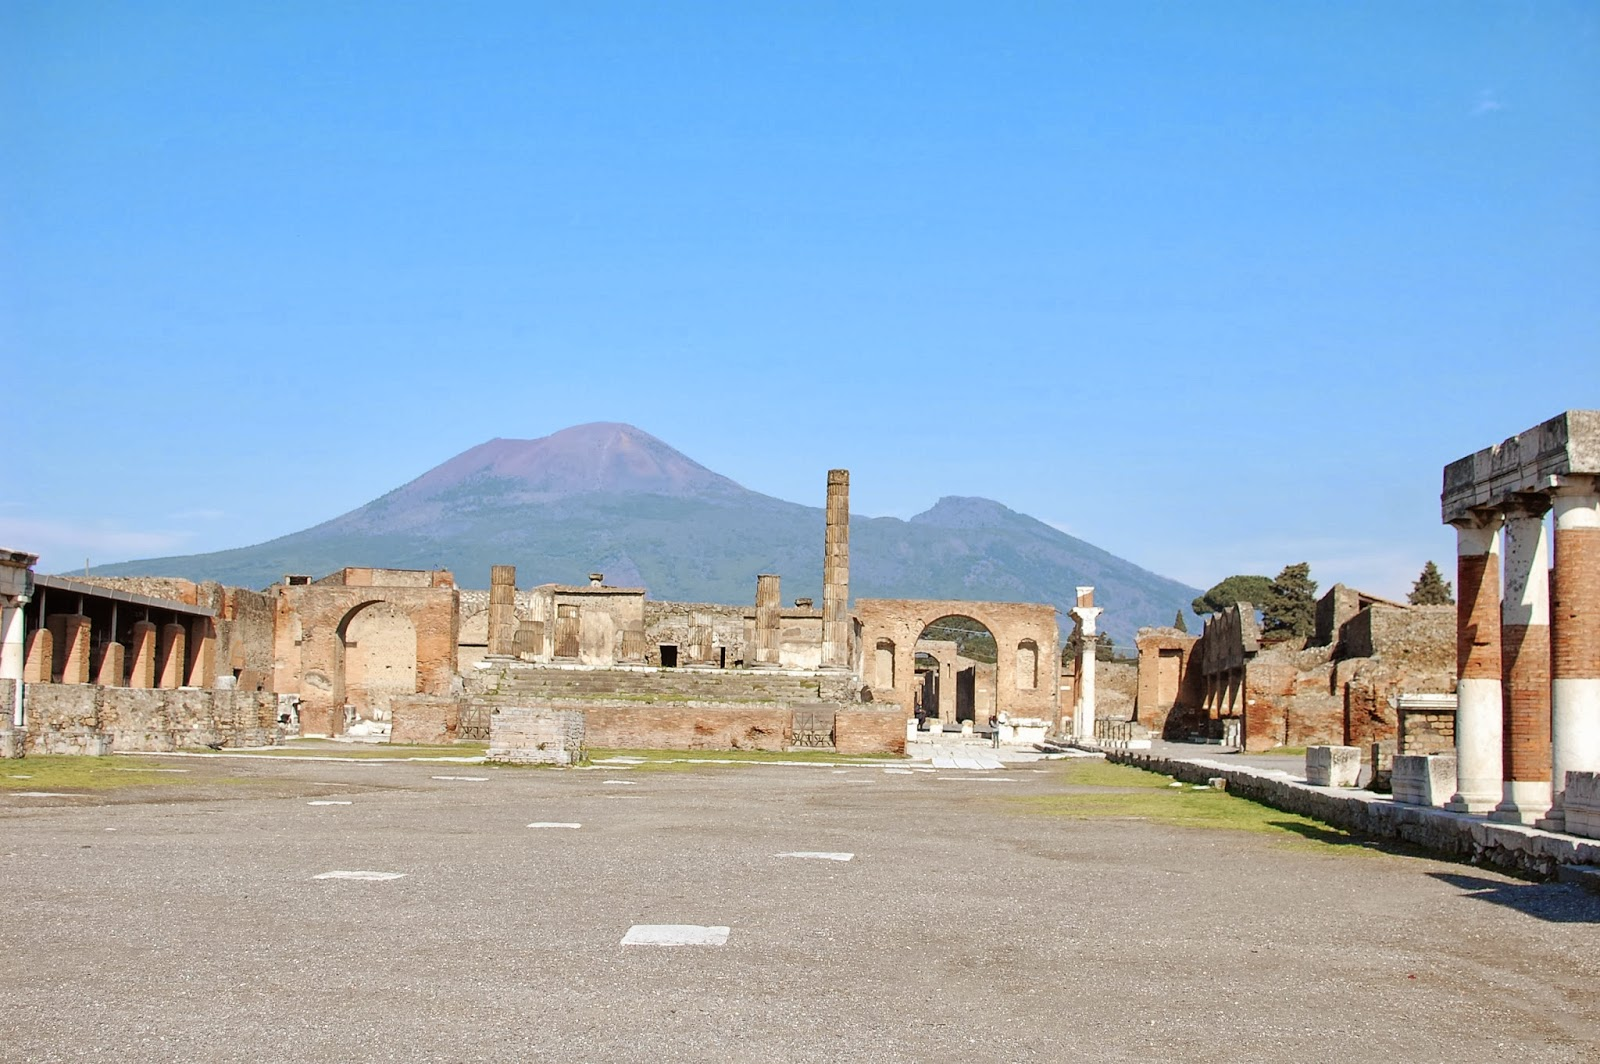
\includegraphics[width=5in]
{vesuvius-pompei.jpg}
\caption{View of Mount Vesuvius from
  Pompeii}
\label{fig-pomp}
\end{figure}

\begin{figure}[h!]
\centering
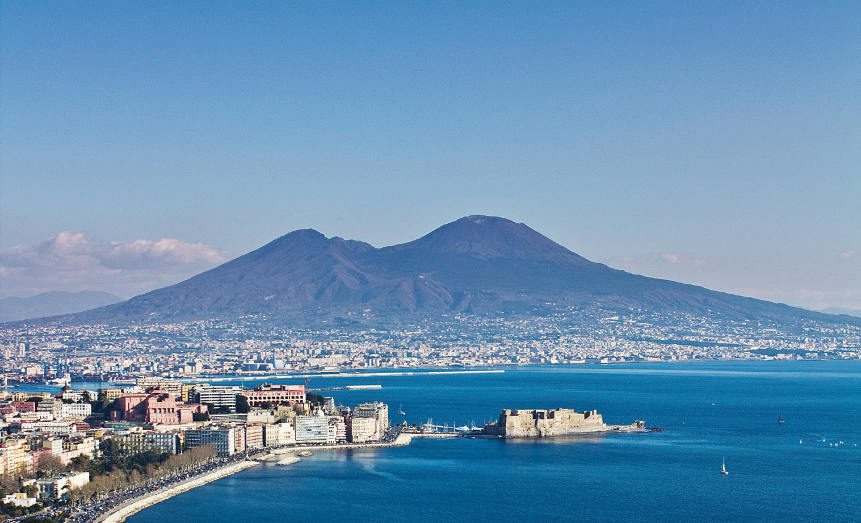
\includegraphics[width=5in]
{vesuvius-bay-of-naples.jpg}
\caption{Mount Vesuvius and Bay of Naples}
\label{fig-naples}
\end{figure}


\newpage
\setcounter{tocdepth}{10}
\tableofcontents
%\include{tempo}
\chapter*{Foreword}
\addcontentsline{toc}{chapter}{Foreword}

Welcome to Bayesuvius! a proto-book uploaded to github.

A different Bayesian network is discussed
 in each chapter. Each chapter title is 
the name of a Bnet. Chapter titles are
 in alphabetical order.

This is a volcano in its early stages.
 First version uploaded to a github repo 
called Bayesuvius on June 24, 2020. 
First version only covers 2 Bnets
(Linear Regression and GAN). 
I will add more chapters periodically.
 Remember, this is a moonlighting effort 
so I can't do it all at once.

For any questions about notation, 
please go to Notational Conventions section.

Requests and advice are welcomed.


\bigskip
\noindent Thanks for reading this

\noindent Robert R. Tucci

\noindent www.ar-tiste.xyz
\bigskip
\\
\noindent{\bf ADDENDA}
\begin{itemize}
\item{\bf August 15, 2021:} At 
this point in time, the book 
has grown to 67 Chapters and 433 pages.
Today, I am self-publishing it as an ebook
at Amazon and similar outlets. It
will still be free.
\end{itemize}


\chapter{Navigating 
the ocean of Judea Pearl's Books}
%\addcontentsline{toc}{chapter}{Navigating the ocean of Judea Pearl's Books}

\label{ch0-nav-pearl}
Many
of the
greatest ideas 
in the bnet field 
were invented by Judea Pearl
and his collaborators.
Thus, this book is 
heavily indebted to
those great scientists.
Those ideas have had no clearer
and more generous 
expositor than Judea Pearl
himself.

Pearl has written
4 books that I have used
in writing Bayesuvius.
His 
1988 book Ref.\cite{pearl-1988book}
dates back to his pre-causal period.
That book I used to learn
about topics such as
d-separation, belief propagation,
Markov-blankets, and noisy-ORs.
3 other books that  he  wrote later,
in his causal period, 
are:
\begin{enumerate}
\item
In 2000 (1st ed.), and 2013 (2nd ed.),
Pearl published what
is so far
his most technical
and exhaustive book
on the subject of causality,
Ref.\cite{pearl-2013book}.
\item
In 2016,
he released 
together
with Glymour and Jewell,
a less advanced ``primer"
on causality, Ref.\cite{pearl-primer}.
\item
In 2018, 
he released 
together with
Mackenzie his
lovely  ``The Book of Why",
 Ref.\cite{book-why}.
\end{enumerate}
Those 3 books I used to learn
about causality topics
such as Do Calculus,
backdoor and frontdoor
adjustment formulae,
linear 
deterministic 
bnets with exogenous noise,
and counterfactuals.

A micro poem written by me
to celebrate Judea Pearl and 
his work:
 
\section*{I, Robot}
\begin{verse}
Let other robots {\tt talk()},\\
while I,\\
{\tt talk()}, {\tt do()} and {\tt imagine()}.
\end{verse}

\chapter{CI-2-3 track}
%\addcontentsline{toc}{chapter}{CI-2-3 track}
\label{ci-track}

\begin{figure}[h!]
\centering
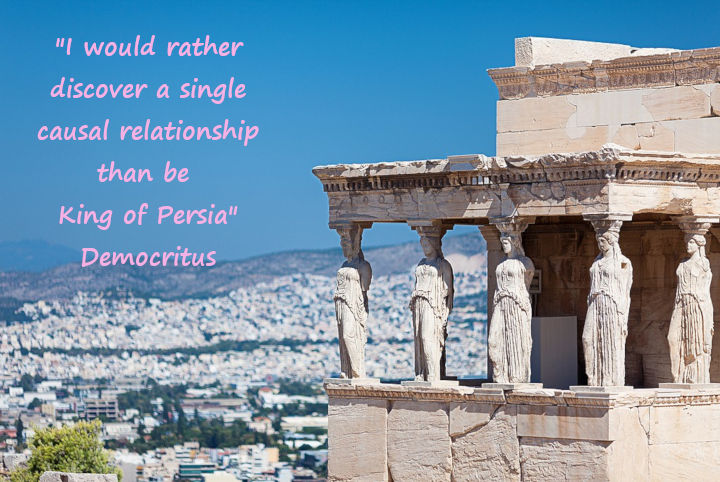
\includegraphics[width=6in]
{democritus-acropolis-caryatids.jpg}
\caption{Democritus quote, Acropolis Caryatids background}
\label{fig-democritus}
\end{figure}

\begin{figure}[h!]
\centering
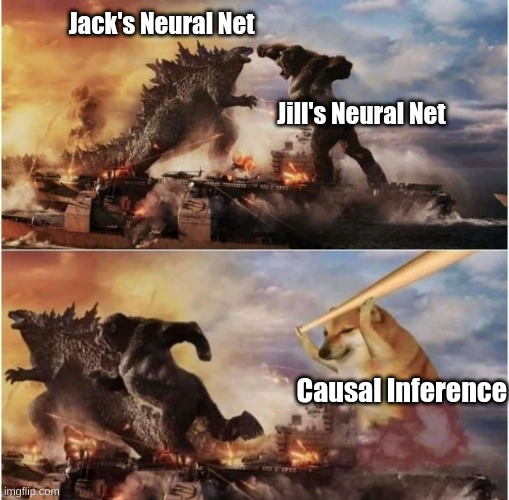
\includegraphics[width=5in]
{godzilla-kk-doge-nn-ci.jpg}
\caption{CI meme}
\label{fig-godzilla-kk-doge}
\end{figure}

\begin{figure}[h!]
\centering
\includegraphics[width=6in]
{pearl-ijcai-2022.jpg}
\caption{Slide from Pearl talk at IJCAI-2022. 
Putting the joking 
of Fig.\ref{fig-godzilla-kk-doge} aside, 
let me emphasize that CI advocates 
are not trying to vanish
NNs from AI. To us,
NNs and bnets
are different tools, like 
hammer and saw. 
We believe AI should use both tools.
For those
who are trying to do
CI using a NN instead of a
bnet, it looks to me like you are
trying to use a hammer
to cut wood. Why don't you cut with 
a saw instead?
As Pearl says in this slide,
CI elevates Data Science
from Deep Learning (curve-fitting) to 
Deep Understanding. }
\label{fig-deep-understanding}
\end{figure}


As discussed in Chapter \ref{ch-counterf},
Judea Pearl has proposed 3 rungs
of Causal Inference (CI).
This book covers all 3 rungs.

Confusingly,
it has become common to use the term
CI to refer to only the highest
2 rungs of the CI hierarchy; i.e,
rung 2 (do operations)
and rung 3 (imagining/counterfactual thinking).
Also confusingly, rung 1
uses causal diagrams and
is often referred to as ``inference",
so it could reasonably have been defined as the whole
of CI, but Pearl has defined
the CI hierarchy to include two more rungs.
To patch over this linguistic confusion,
I sometimes refer to rung 1 as ``prediction",
or as ``predictive inference"
instead of calling it merely ``inference".
Also, when I want to be precise,
I use the term ``CI-2-3" to
refer to CI restricted to only rungs 2 and 3.


Here is a subset of chapters
that I call
the CI-2-3 track,
that are devoted mostly to rungs 2 and 3.


\begin{enumerate}
\item \nameref{ch-bdoor}
\item \nameref{ch-berkson}
\item \nameref{ch-counterf}
\item \nameref{ch-dec-2-3}
\item \nameref{ch-did}
\item \nameref{ch-do-calc}
\item \nameref{ch-do-calc-proofs}
\item \nameref{ch-dsep}
\item \nameref{ch-dsep-lden}
\item \nameref{ch-fwl-theo}
\item \nameref{ch-fdoor}
\item \nameref{ch-g-formula}
\item \nameref{ch-good-causal-fit}
\item \nameref{ch-granger-c}
\item \nameref{ch-inst-ineq}
\item \nameref{ch-instrumental}
\item \nameref{ch-late}
\item \nameref{ch-mediation}
\item \nameref{ch-mendelian-rand}
\item \nameref{ch-meta-learners}
\item \nameref{ch-modi-treat}
\item \nameref{ch-personalized-exp-util}
\item \nameref{ch-personalized}
\item \nameref{ch-pot-out}
\item \nameref{ch-reg-dis}
\item \nameref{ch-sb-removal}
\item \nameref{ch-simpson}
\item \nameref{ch-survival}
\item \nameref{ch-syn-con}
\item \nameref{ch-targeted-est}
\item \nameref{ch-transport}
\item \nameref{ch-uplift}
\end{enumerate}



\chapter*{Notational Conventions and Preliminaries}
\addcontentsline{toc}{chapter}{Notational Conventions and Preliminaries}

\label{ch0-conventions}
\section{Some abbreviations frequently
used throughout this book}

\begin{itemize}
\item
bnet= Bnet= Bayesian Network
\item
CPT = Conditional Probabilities Table,
 same as TPM
\item
DAG = Directed Acyclic Graph
\item
i.i.d.= independent identically
distributed.
 \item
 RCT= Randomized Controlled Trial,
a.k.a. A/B testing.

\item
TPM= Transition Probability Matrix,
same as CPT

\end{itemize}

\section{${\cal N}(!a)$}
$\caln(!a)$ will denote
a normalization constant that does not depend
on $a$. For example, $P(x)=\caln(!x)e^{-x}$
where $\int_0^\infty dx \;P(x)=1$.

\section{One hot vector}
A {\bf one hot  vector}
is a vector with all entries
equal to zero with
the exception of a single entry which is one.
A {\bf one cold vector}  is a vector with all entries
equal to one with the exception of  a
single entry which is zero.
For example, if $x^n=(x_0, x_1, \ldots,
x_{n-1})$ and
$x_i=\delta(i,0)$ then $x^n$ is one hot.

Two types of
sets that one frequently encounters
are {\bf categorical sets} (a.k.a. ``nominal sets", i.e.,
sets with ``named" elements, with elements given a ``nomme")
and {\bf numerical sets} (a.k.a. ``ordinal sets", i.e., sets
 with ``ordered"
elements).
For example, $\{1,2,5\}$ is a numerical set
because its elements have a natural order,
and $\{\text{cat, dog, bird}\}$ is a  categorical set
because its elements don't have a natural order.

In Machine Learning (ML),
one often encodes categorical sets as one-hot vectors.
For example, suppose we have 4 binary registers (i.e., nodes)
 $x_3, x_2,x_1, x_0$
and  the categorical set $\{\text{cat, dog, canary}\}$.
Then a possible {\bf one-hot encoding}
of the set
is cat=0001, dog=0010 and canary=0100.
This differs from
a {\bf binary encoding} of the set such as
cat=0000, dog=0001, canary=0011.
Clearly, a binary encoding requires
fewer registers than a one-hot
encoding to
encode the same set,
and the one-hot encoding
of a set with $n$ elements requires
$n$ or more registers.

\section{Special sets}
Define $\ZZ, \RR, \CC$ to be
 the integers, real numbers
 and complex numbers, respectively.

For $a<b$, define $\ZZ_I$
to be the integers in the
interval $I$, where
$I=[a,b],[a,b),(a,b],(a,b)$
(i.e, $I$ can be closed or
 open on either side).

$A_{>0}=\{k\in A: k>0\}$ for $A=\ZZ, \RR$.

\section{Kronecker
delta function}

 For $x,y$ in discrete set $S$,
\beq
\delta(x,y)=\left\{
\begin{array}{l}
1\;{\rm if}\; x=y
\\
0 \;{\rm if}\; x\neq y
\end{array}
\right.
\eeq

\section{Dirac delta function}
 For $x,y\in\RR$,
\beq
\int^{+\infty}_{-\infty}dx\;\delta(x-y)f(x)=f(y)
\eeq

\section{Indicator function
(a.k.a. Truth function)}
\beq
\indi(\cals)=\left\{
\begin{array}{l}
1\;{\rm if\; \cals\; is\; true}
\\
0 \;{\rm if \;\cals\; is \;false}
\end{array}
\right.
\eeq
For example, $\delta(x,y)=\indi(x=y)$.

\section{Majority function}
The {\bf majority function}  is defined as follows.

\beq
\begin{array}{ll}
{\tt majority}(L)=&
\text{ most common element of  list $L$}
\\
&\text{(ties resolved by chance)}
\end{array}
\eeq
Note that the majority function
acts on lists, not sets. By definition,
all elements of a set appear only once in the set.
${\tt majority}(L)$
is usually
used when the elements of
$L$ are categorical (i.e., not real numbers).
When they are real numbers,
it makes more sense to use, instead of
${\tt majority}(L)$, a simple average
of the elements of $L$.


\section{Underlined letters
 indicate random variables}
Random variables will be indicated by
underlined letters and their values
by non-underlined letters.
 Each node of a bnet will be
 labelled by a random variable.
 Thus, $\rvx=x$ means that node
$\rvx$ is in state $x$.

It is more
conventional to
use an upper
case letter to
indicate
a random
variable
and a lower case letter
for its state.
Thus, $X=x$ means that
random variable
$X$ is in state $x$.
However,
we have
opted
in this
book to
avoid
that notation,
because
we often
want to define
certain lower
case letters
to be random variables
or, conversely, define certain upper
case letters to
be non-random variables.

\section{Probability distributions}
 $P_\rvx(x)=P(\rvx=x)=P(x)$ is the probability that random variable $\rvx$ equals $x\in S_\rvx$. $S_\rvx$ is the set of states (i.e., values) that $\rvx$ can assume and $n_\rvx = |S_\rvx|$ is the size (a.k.a. cardinality) of that set. Hence,
\beq
\sum_{x\in S_\rvx}P_\rvx(x)=1
\eeq

\hrule
\beq
P_{\rvx,\rvy}(x,y)=P(\rvx=x, \rvy=y)=P(x,y)
\eeq
\beq
P_{\rvx|\rvy}(x|y)=P(\rvx=x| \rvy=y)=P(x|y)=\frac{P(x,y)}{P(y)}
\eeq



\section{Discretization
of continuous
probability distributions}

The TPM of a node
of a bnet can be either a discrete or
a continuous probability distribution.
To go from continuous to discrete, one
replaces integrals over states of a node
 by sums over new states, and Dirac delta
functions by Kronecker delta functions.
 More precisely, consider a function
$f: [a, b]\rarrow \RR$. Express
 $[a,b]$ as
a union of
small, disjoint (except for
one point) closed sub-intervals (bins) of
length $\Delta x$.
Name one point
in each bin to be the representative of that bin,
and  let $S_\rvx$ be the
set of all the bin representatives. This is called
discretization or binning. Then

\beq
\frac{1}{(b-a)}
\int_{[a,b]} dx \; f(x)\rarrow
\frac{\Delta x}{(b-a)} \sum_{x\in S_\rvx}f(x)
=
\frac{1}{n_\rvx} \sum_{x\in S_\rvx}f(x)
 \;.
\eeq
Both sides of last equation are 1 when $f(x)=1$.
 Furthermore, if $y\in S_\rvx$, then

\beq
\int_{[a,b]} dx \; \delta(x-y)f(x)=f(y)
\rarrow \sum_{x\in S_\rvx}\delta(x,y)f(x)
=f(y)
\;.
\eeq

As usual in this book, let $S_\rvx$ denote the set of
values that the random variable $\rvx$ can take.
When $S_\rvx\subset \RR$,
we will assume that $S_\rvx$
for a probability distribution $P(x)$
can be either a discrete or a continuous
subset of $\RR$.\footnote{By a ``continuous set" we
mean a finite set of intervals
 each of which has non-zero length.}
When $S_\rvx$ is a discrete subset of $\RR$, $P(x)$
will denote a probability distribution
for which $\sum_{x\in S_\rvx}P(x)=1$, whereas when
$S_\rvx$ is continuous, $P(x)$ will denote
a probability density
for which $\int_{x\in S_\rvx}dx\; P(x)=1$.

\section{Samples,
i.i.d. variables}
\beq
\vec{x}= (x[0], x[1], x[2] \ldots,
 x[nsam(\vecx)-1])=x[:]
\eeq

 $nsam(\vecx)$ is the number of samples
 of $\vecx$.
$\rvx[\sigma]\in S_\rvx$ are
 i.i.d. (independent identically distributed)
samples with

 \beq
x[\sigma]\sim P_\rvx\;\;({\rm i.e.}\; P_{\ul{x[\sigma]}}=P_\rvx)
\eeq

\beq
P(\rvx=x)=\frac{1}{nsam(\vecx)}\sum_\sigma \indi(x[\sigma]=x)
\eeq
Hence, for any $f:S_\rvx\rarrow \RR$,
\beq
\sum_x P(\rvx=x)f(x)
=\frac{1}{nsam(\vecx)}\sum_\sigma f(x[\sigma])
\eeq


If we use two sampled variables, say $\vecx$ and $\vecy$,
in a given bnet, their number of samples
$nsam(\vecx)$ and $nsam(\vecy)$ need not be equal.

\hrule
\beq
P(\vecx) = \prod_\sigma P(x[\sigma])
\eeq

\beq
\sum_\vecx = \prod_\sigma\sum_{x[\sigma]}
\eeq

\beq
\partial_\vecx =
[\partial_{x[0]}, \partial_{x[1]},\partial_{x[2]}, \dots, \partial_{x[nsam(\vecx)-1]}]
\eeq

\hrule
\beqa
P(\vecx)&\approx& [\prod_x P(x)^{P(x)}]^{nsam(\vecx)} \\
&=& e^{nsam(\vecx)\sum_x P(x)\ln P(x)}\\
&=& e^{-nsam(\vecx)H(P_\rvx)}
\eeqa

\section{Expected Value and Variance}

Given a random variable
 $\rvx$ with states $S_\rvx$ and
a function $f:S_\rvx\rarrow \RR$, define

\beq
E_\rvx[f(\rvx)]=
E_{x\sim P(x)}[f(x)] = \sum_x P(x) f(x)
\eeq

\beqa
Var_\rvx[f(\rvx)]&=& E_\rvx
\left[(f(\rvx)-E_\rvx[f(\rvx)])^2\right]
\\
&=&
E_\rvx[f(\rvx)^2]-(E_\rvx[f(\rvx)])^2
\eeqa

\beq
E[\rvx]=E_\rvx[\rvx]
\eeq

\beq
Var[\rvx]=
Var_\rvx[\rvx]
\eeq



\section{Conditional Expected Value}

Given a random variable $\rvx$ with states $S_\rvx$, a random variable $\rvy$ with states $S_\rvy,$ and a function $f:S_\rvx\times S_\rvy\rarrow \RR$, define

\beq
E_{\rvx|\rvy}[f(\rvx, \rvy)]=
\sum_x P(x|\rvy) f(x, \rvy)
\;,
\eeq

\beq
E_{\rvx|\rvy=y}[f(\rvx, y)]=
E_{\rvx|y}[f(\rvx, y)]= \sum_x P(x| y) f(x, y)
\;.
\eeq
Note that

\beqa
E_\rvy[E_{\rvx|\rvy}[f(\rvx, \rvy)]]&=&
\sum_{x,y}P(x|y)P(y)f(x,y)
\\&=&
\sum_{x,y}P(x,y)f(x,y)
\\&=&
E_{\rvx, \rvy}[f(\rvx, \rvy)]
\;.
\eeqa



\section{Notation
for covariances}
Consider two random variables $\rvx, \rvy$.

\begin{itemize}
\item
Mean value of $\rvx$
\beq
\av{\rvx}=
E_\rvx[\rvx]
\eeq

\item
Signed distance of $\rvx$ to its mean value
\beq
\Delta \rvx = \rvx - \av{\rvx}
\eeq

\item
Covariance of $(\rvx, \rvy)$
\beq
Cov(\rvx, \rvy)=\av{\rvx, \rvy}=
\av{\Delta \rvx \Delta \rvy}
=
\av{\rvx\rvy}-\av{\rvx}\av{\rvy}
\eeq

$\av{\rvx, \rvy}$ is symmetric
(i.e., $\av{\rvx, \rvy}=\av{\rvy, \rvx}$)
and bilinear (i.e.,
$\av{\sum_i \alp_i\rvx_i, \rvy}
=
\sum_i\alp_i\av{\rvx_i, \rvy}$, where
$\alp_i\in \RR$
are non-random scalars
and $\rvx_i, \rvy\in\RR$ are
real-valued random
variables.)

\item
Variance of $\rvx$
\beq
Var(\rvx)=\av{\rvx, \rvx}
\eeq

\item
Standard deviation or $\rvx$
\beq
\sigma_\rvx=\sqrt{\av{\rvx, \rvx}}
\eeq

\item
Correlation Coefficient of $(\rvx, \rvy)$
\beq
\rho_{\rvx, \rvy}=
\frac{\av{\rvx, \rvy}}
{\sqrt{\av{\rvx, \rvx}\av{\rvy, \rvy}}}
\eeq
\end{itemize}

\section{Conditional Covariance}
Let $\rvx, \rvy, \rva$
be random variables.
The covariance $Cov(\rvx, \rvy|\rva)$
of $\rvx$ and $\rvy$
given $\rva$, is defined
the same
way as $Cov(\rvx, \rvy)$,
except that all
expected values are
conditioned on $\rva$.



\beq
Cov(\rvx, \rvy|\rva)=
\av{\rvx, \rvy}_{|\rva}
=
\av{(\rvx-\av{\rvx}_{|\rva})
(\rvy-\av{\rvy}_{|\rva})}_{|\rva}
\eeq
where

\beq
\av{\rvx}_{|\rva}=E_{\rvx|\rva}[\rvx]
\;.
\eeq

\section{Law of Total Variance}

\begin{claim}
Suppose $P:S_\rvx\times S_\rvy\rarrow [0,1]$
is a probability distribution.
Suppose $f:S_\rvx\times S_\rvy\rarrow \RR$
 and $f=f(x,y)$. Then
\beq
Var_{\rvx, \rvy}(f)=
E_\rvy[Var_{\rvx|\rvy}(f)]
+
Var_\rvy(E_{\rvx|\rvy}[f])
\;.
\eeq
In particular,
\beq
Var_{\rvx}(x)=
E_\rvy[Var_{\rvx|\rvy}(x)]
+
Var_\rvy(E_{\rvx|\rvy}[x])
\;.
\eeq

\end{claim}
\proof

Let
\beq
A=\sum_y P(y)\left(\sum_x P(x|y)f\right)^2
\;.
\eeq
Then

\beqa
Var_{\rvx, \rvy}(f)&=& \sum_{x,y}P(x,y)f^2 -
\left( \sum_{x,y} P(x,y) f\right)^2
\\
&=&
\left\{
\begin{array}{l}
\sum_{x,y}P(x,y)f^2
-A
\\
+\left(A-\left( \sum_{x,y} P(x,y) f\right)^2\right)
\end{array}
\right.
\eeqa

\beqa
E_\rvy[Var_{\rvx|\rvy}(f)]
&=&
\sum_y P(y)\left(\sum_x P(x|y)f^2
-
\left(\sum_x P(x|y)f\right)^2
\right)
\\
&=&
\sum_{x,y}P(x,y)f^2
-A
\eeqa

\beqa
Var_\rvy(E_{\rvx|\rvy}[f])
&=&
\sum_y P(y)
\left(\sum_x P(x|y)f\right)^2
-\left(
\sum_y P(y)\sum_xP(x|y)f
\right)^2
\\
&=&
A-\left( \sum_{x,y} P(x,y) f\right)^2
\eeqa
\qed





\section{Normal Distribution}


For $x, \mu, \sigma\in \RR$,
$\sigma >0$, we define the Normal Distribution
(see Fig.\ref{fig-norm-dist}) by

\beq
\caln(x; \mu, \sigma^2)=
\frac{1}{\sigma\sqrt{2\pi}}
e^{-\;\frac{1}{2}\left(
\frac{x-\mu}{\sigma}\right)^2}
\;.
\eeq

For a {\bf standard deviation}
$\s$, the {\bf precision} $\tau$
is defined as $\tau=\frac{1}{\s^2}$.

\begin{claim}
If

\beq
\rvx_1\sim \caln(\mu_1, \s^2_1)
\eeq
and

\beq
\rvx_2\sim \caln( \mu_2, \s^2_2)
\eeq
then
\beq
\rvx=\rvx_1 +\rvx_2 \sim \caln(\mu_1 + \mu_2, \s^2_1 + \s^2_2)
\;.
\eeq
\end{claim}
\proof

\beqa
P(\rvx=x)&=&\caln(!x)
\int_{-\infty}^{+\infty}dx_2\;
P(\rvx_1 + \rvx_2 = x|\rvx_2=x_2)P(x_2)
\\
&=&\caln(!x)
\int_{-\infty}^{+\infty}dx_2\;
\caln(x-x_2;\mu_1, \s^2_1)
\caln(x_2;\mu_2, \s^2_2)
\\
&=&
\caln(x;\mu_1 +\mu_2; \s^2_1+\s^2_2)
\eeqa
\qed

\begin{figure}[h!]
\centering
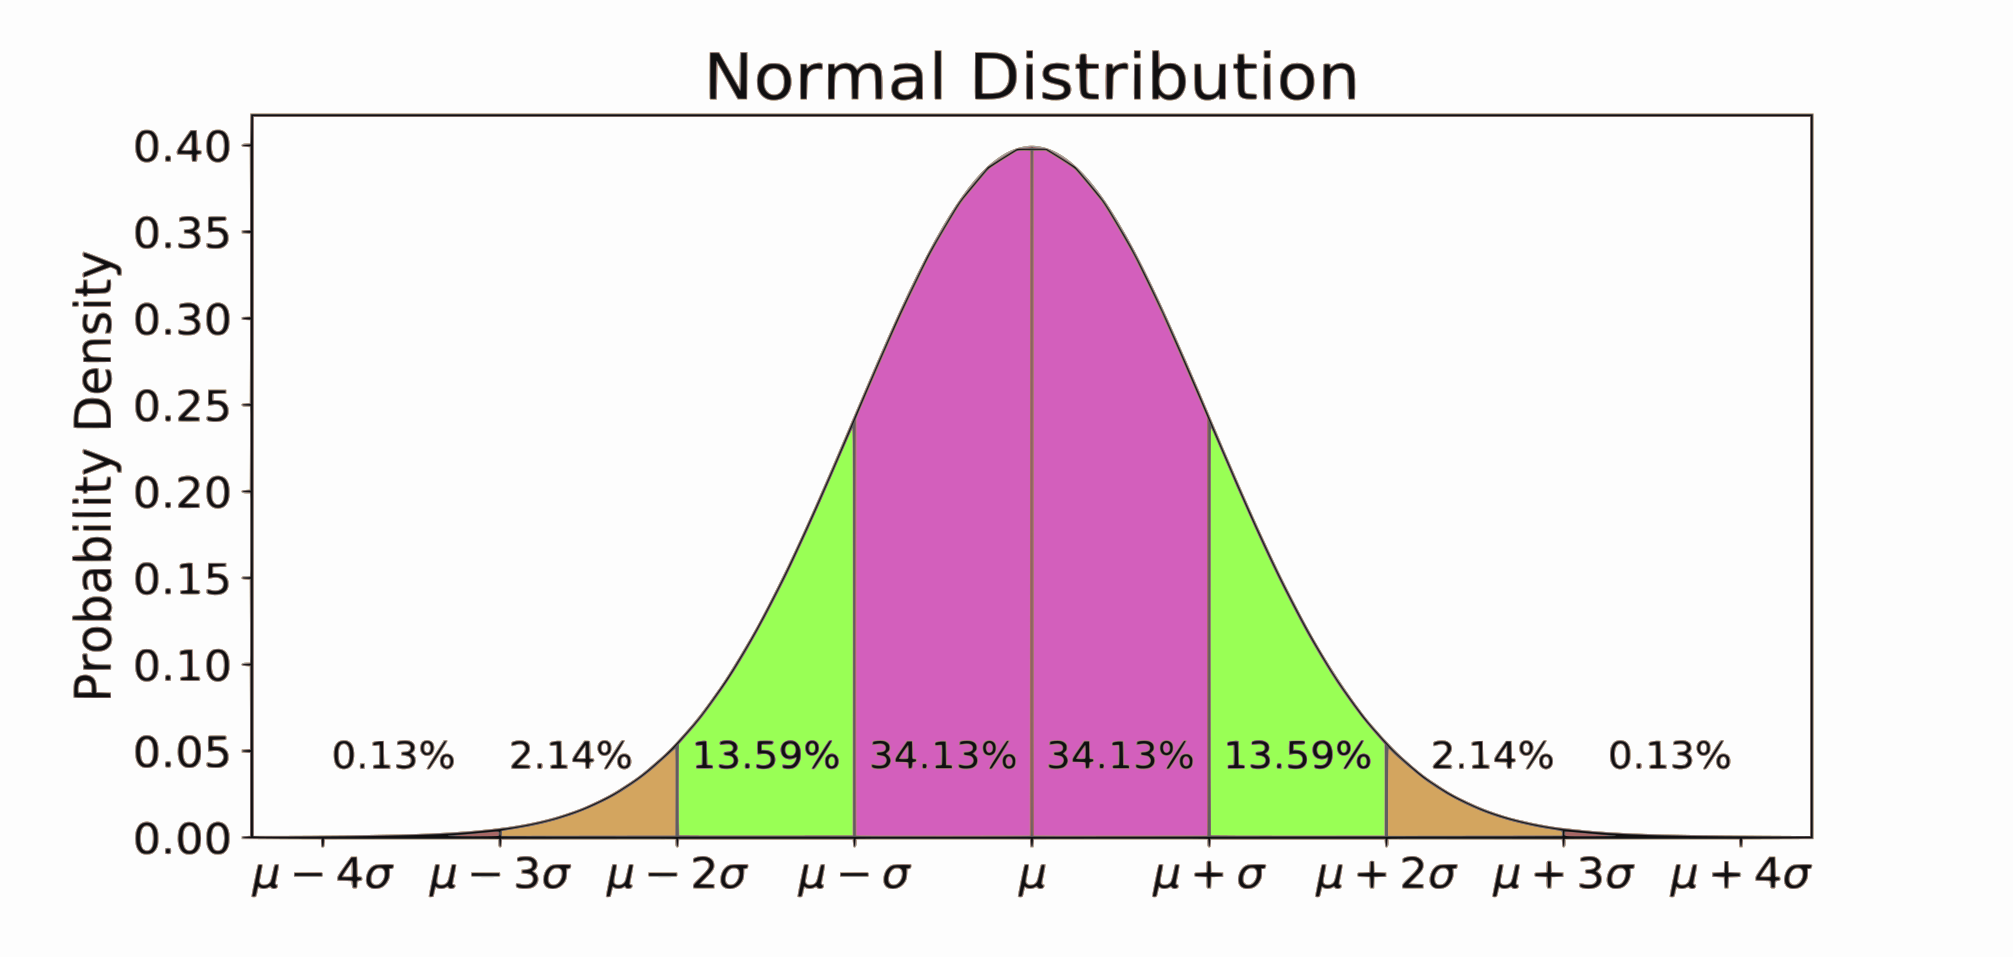
\includegraphics[width=5in]
{conventions/normal-dist.png}
\caption{Normal Distribution
$\caln(x;\mu, \s^2)$.}
\label{fig-norm-dist}
\end{figure}

The {\bf Standard Normal Distribution} $P_{SND}(x)$
and its cumulative distribution $\Phi(x)$ are defined by

\beq
P_{SND}(x)=\caln(x; \mu=0, \s=1)
\eeq

\beq
\Phi(x) = \int_{-\infty}^x dx'\;P_{SND}(x')
\eeq

The {\bf error function} ${\rm erf}:\RR\rarrow [-1,1]$
is defined by
\beq
{\rm erf}(x) = \frac{2}{\sqrt{\pi}}
\int_0^x du \; e^{-\;\frac{u^2}{2}}
\eeq

Note that

\beq
\Phi(x)= \frac{1}{2} + \frac{1}{2}{\rm erf}(x)
\label{eq-Phi-erf}
\eeq
Eq.(\ref{eq-Phi-erf})
is interpreted geometrically in Fig.\ref{fig-erf}.

\begin{figure}[h!]
\centering
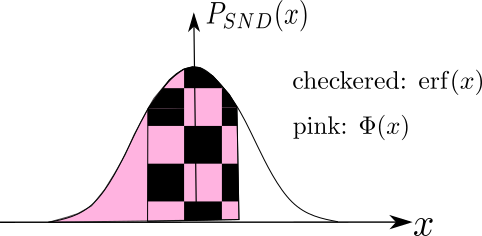
\includegraphics[width=2.8in]
{conventions/erf.png}
\caption{Plot of Standard
Normal Distribution $P_{SND}(x)$.
 Values of ${\rm erf}(x)$ and $\Phi(x)$
 equal indicated areas.}
 \label{fig-erf}
\end{figure}
\section{Uniform Distribution}
For $a<b$, $x\in [a,b]$

\beq
\calu(x;a,b) =
\frac{1}{b-a}
\eeq

\section {Softmax function
(a.k.a. Boltzmann Distribution)}

The Softmax function
 is defined by
\beq
P(x_i
|x.)=\frac{e^{x_i}}{\sum_i e^{x_i}}=
\softmax(x.)_i
\label{eq-softmax}
\eeq
The
Boltzmann distribution is defined as

\beq
P(\rvE_a=E_a)=\frac{\exp(-\;\frac{E_a}{kT})}{\sum_{a}
\exp(-\;\frac{E_{a}}{kT})}=
P(\frac{-E_a}{kT}|E.)\eeq
for a system with energies $E_a$
and temperature $T$,
where $k$
is Boltzmann's constant.

The function
softmax() is called softmax because if we
approximate the exponentials,
 both in the numerator and denominator
of Eq.(\ref{eq-softmax}),
by the largest one
of them or zero,
we get

\beq
\softmax(x.)_i\approx \indi(i=\argmax_k x_k)
\;.
\eeq
Thus, softmax($x.$)
returns a continuous
function that approximates a one-hot vector
that is 1 at the
$i$th
component, where
$i=\argmax_k(x_k)$,
and zero at the other components.

Note that
\beq
\pder{\ln P(x_i|x)}{x_a}
=
\pder{}{x_a}\ln\left[
\frac{e^{x_i}}{\sum_i e^{x_i}}
\right]
=
\delta(a,i)
-
P(x_a|x)
\eeq

For 2 variables $x_0, x_1$,
\beqa
P(x_0|x.)&=&
\frac{e^{x_0}}{e^{x_0} + e^{x_1}}\\
&=&\smoid(x_0-x_1)
\;,
\eeqa

\beq
P(x_1|x.)=\smoid(x_1-x_0)
\;.
\eeq

\section{Sigmoid and log-odds functions}
\label{sec0-smoid}
The {\bf sigmoid (a.k.a. exp-it,  logistic) function} smoid:$\RR\rarrow [0,1]$
is defined by
\beq
\smoid(x)=
\frac{1}{1+e^{-x}}
\eeq
$\smoid()$ is monotonically
increasing with $\smoid(-\infty)=0$,
$\smoid(0)=1/2$
and $\smoid(+\infty)=1$.
Note that for $x<<0$, $\smoid(x)\approx e^x$, which
is why ``smoid" is also called ``expit".

\beqa
\smoid(x)+\smoid(-x)&=&
\frac{1}{1+e^{-x}}+\frac{1}{1+e^x}\\
&=&\frac{2+e^x+e^{-x}}{2+e^x+e^{-x}}
\\&=&1
\eeqa


The {\bf log-odds (a.k.a. log-it) function}
lodds:$[0,1]\rarrow \RR$ is defined by

\beq
{\rm lodds}(p)=\ln\frac{p}{1-p}
\eeq
Note that for $0< p<<1$, $\lodds(x)\approx \ln p$,
which is why ``lodds" is also called ``logit".

Note that for $x<<1$, $\smoid(x)\approx e^x<<1$,
so $\lodds(e^x)\approx \ln(e^x)=x$.
More generally, it
is easy to check that for any $p\in[0,1]$ and $x\in \RR$,
\beq
\lodds[\smoid(x)]=x
\eeq

\beq
\smoid [\lodds(p)] =p
\eeq
Hence,
$\lodds()$ is the inverse of $\smoid()$ and vice-versa.

\begin{claim}
\beq
\smoid'(x)=\smoid(x)[1-\smoid(x)]
\eeq

\beq
\smoid''(x)=\smoid'(x)[1-2\smoid(x)]
\eeq
\end{claim}
\proof

In this proof, we will
abbreviate $\smoid(x)$ by $s(x)$.
\beq
1-s(x)=1 -\;\frac{1}{1+e^{-x}}=
\frac{e^{-x}}{1+e^{-x}}
\eeq

\beq
s'(x)= \frac{e^{-x}}{(1+e^{-x})^2}
=s(x)[1-s(x)]
\eeq

\beqa
s''(x)&=&s'(x)[1-s(x)]
+
s(x)(-1)s'(x)
\\
&=&
s'(x)[1-2s(x)]
\\
&=&
s(x)[1-s(x)][1-2s(x)]
\eeqa
\qed

\section{Estimand, Estimator (curve-fit, cfit), Estimate, Bias}
\label{sec0-estimand}
For an {\bf estimand} $\theta$,
an {\bf estimator (a.k.a. curve fit,
cfit)} $\ul{\HAT{\theta}}$
gives {\bf estimate} $E[\ul{\HAT{\theta}}(\theta)]=\theta+b$
with {\bf bias} $b$.
We say this estimate is an {\bf unbiased estimate}
if $b=0$.

Note that, strictly
speaking, an estimator is a function
waiting to be averaged over
and denoted by a letter with a hat,
whereas an estimate is a real number
denoted by a letter without a hat.
Unfortunately, the
words ``estimator" and
``estimate" are often used interchangeably,
as if they were synonyms.
And often the estimate $\theta + b$
is denoted by a letter with a hat too.
In some sense, an estimator is an estimate
of a curve, so it's understandable that
the terms ``estimator" and ``estimate"
are used synonymously.
In this book, we will bow to traditional
practice and
also use
the terms ``estimator" and ``estimate"
synonymously, and use a letter
with a hat to denote either of them.
This is not
ambiguous as long as we don't
use the same letter with a
hat to denote two different quantities, of course.
When we need to distinguish semantically
between the real value and the function,
we will call the function a cfit,
and the real value the estimate.

\section{Maximum Likelihood Estimate,
Likelihood Ratio Test}
\label{sec0-likelihood-ratio}

Given a bnet, let $P(x|\theta)$
be its full joint probability distribution,
where
$x$ denotes the joint state
of all the nodes and $\theta$
denotes all the parameters.
 $P(x|\theta)$ is often
called the {\bf likelihood function of $\theta$}
and is denoted by

\beq
L(\theta)= P(x|\theta)
\eeq
It's called a likehood of $\theta$
because, even though it's a probability,
it isn't the probability of $\theta$,
but rather of $x$.

The value of $\theta$
that we obtain by maximizing $L(\theta)$
over $\theta$ is called
the
{\bf maximum likelihood
estimate (MLE) of $\theta$}. Let us denote it by
$\HAT{\theta}$. Note that\footnote{``sup" stands for supremum.
It's a generalization of the function $\max()$
to arbitrary sets
that might not be discrete or finite.
If $S$ is a
finite set,
then $\sup_{\theta\in S} f(\theta)=
\max_{\theta\in S} f(\theta)$
for any function $f:S\rarrow \RR$.
Likewise, ``inf" stands for infimum,
and it generalizes the $\min()$ function.}

\beq
\sup_{\theta\in S}L(\theta)=
L(\HAT{\theta})
\eeq


Let $S_0, S_1$ be disjoint sets such that
 $S=S_0\cup S_1$.
We'll say
the {\bf null hypothesis $H_0$} holds
 if $\theta\in S_0$,
and the {\bf alternative hypothesis $H_1$}
holds if
$\theta\in S_1$.
The {\bf likelihood ratio (LR) test statistic}
is defined by


\beq
R=-2\ln
\left(\frac{\sup_{\theta\in S_0}L(\theta)}
{\sup_{\theta\in S}L(\theta)}\right)
\eeq
$R\geq 0$ and $R=0$ if  $S_0=S$.
For some small $c>0$,
if $R<c$, then we reject the alternative hypothesis,
and if $R>c$, we accept it.




If $S_0=\{\theta_0\}$,
then

\beq
R= -2[\ln L(\theta_0) -\ln L(\HAT{\theta})]
\eeq


\section{Mean Square Error (MSE)}

Suppose we are
given $nsam$ samples $y^\s\in\RR$
labeled by an index $\s$,
and a cfit $\haty^\s(a)\in\RR$
that depends on a parameter $a\in\RR$.
Define the {\bf Mean Square
Error (MSE)}
by

\beq
MSE(a) = \frac{1}{nsam}\sum_\s (y^\s-\haty^\s(a))^2
\;.
\eeq
For example, in Linear Regression (LR),
we have $\haty^\s= a_0 + a_1 x^\s$
where $a=(a_0, a_1)$ is a deterministic
parameter.
If the samples $y^\s$
are i.i.d,
then we can also write


\beq
MSE(a)=E_{|a}[(\rvy-\ul{\haty}(a))^2]
\;.
\eeq
and for LR, $\ul{\haty}(a)=a_0+a_1\rvx$.

Define the {\bf residual} $\Delta\rvy$ by:


\beq
\Delta\rvy(a) =\rvy-\ul{\haty}(a)
\;\;\;\text{ (Hence
$\rvy=\ul{\haty} + \Delta\rvy$)}
\eeq

In the rest of this section,
we will discuss the case that
$\haty^\s(a)$ is independent of $x^\s$.
I call
this the {\bf deterministic MSE (D-MSE)}
model.
Note that this
is different from the LR
case where
$\haty^\s(a)$ does depend on $x^\s$.
In LR, we are trying
to fit
a line to a cigar-shaped
2-D scatter plot.
Here, we are just trying
to estimate
the mean value (center of mass)
of a scatter plot.


\begin{claim}
MSE is minimized
over all functions $\haty$ if
\beq
\haty =E_{|a}[\rvy]
\eeq
\end{claim}
\proof

\beq
MSE = E_{|a}[\rvy^2]-2\haty E_{|a}[\rvy]+ \haty^2
\eeq

\beq
0=\frac{d}{d\haty} MSE = 2(-E_{|a}[\rvy]+\haty)
\eeq
Hence,
\beq
\haty =E_{|a}[\rvy]
\eeq
\qed

Sometimes, we will
use the notation
\beq
\haty_{MSE} = E_{|a=a_{MSE}}[\rvy]
\;.
\eeq

\begin{claim}
Suppose $f(a)$
is a function of $a$.
If $\haty=E_{|a}[\rvy]$, then

\beq
E_{|a}[\Delta \rvy]=
E[\Delta \rvy]=0
\eeq



\beq
E_{|a}
\left[\Delta \rvy f(\rva)\right]=
E
\left[\Delta \rvy f(\rva)\right]=0
\eeq
\end{claim}
\proof

\beq
E_{|a}[\Delta\rvy]=
E_{|a}
\left[\rvy-E_{|a}[\rvy]\right]=
E_{|a}[\rvy]-E_{|a}[\rvy]=0
\eeq

\beq
E[\Delta \rvy] =
 E_{\rva}[E_{|\rva}[\Delta\rvy]]=0
\eeq


\beqa
E_{|\rva}
\left[\Delta \rvy f(\rva)\right]
&=&
f(\rva)
\underbrace{E_{|\rva}
[\Delta\rvy]}_{=0}
\eeqa

\beq
E[\Delta \rvy f(\rva)]
=E_\rva[E_{|\rva}[\Delta\rvy f(\rva)]]=0
\eeq
\qed


\begin{claim}
If $\haty=E_{|a}[\rvy]$, then

\beq
\av{\Delta\rvy, \haty}_{|a}
=0
\label{eq-mse-uncorr}
\eeq

\beq
Var_{|a}[\rvy]
=
Var_{|a}[\haty]
+
Var_{|a}[\Delta\rvy]
\eeq
The same results hold
without the conditioning on $a$.
\end{claim}
\proof

\beqa
\av{\Delta\rvy, \ul{\haty}}_{|a}
&=&
\underbrace{E_{|a}[\Delta\rvy \;\underbrace{\ul{\haty}}
_{f(\rva)}]
}_{=0}
-
\underbrace{E_{|a}[\Delta\rvy]}_{=0}
E_{|a}[ \ul{\haty}]
\eeqa

\beqa
Var_{|a}[\rvy]
&=&
\av{\haty +\Delta\rvy, \haty +\Delta\rvy}_{|a}
\\
&=&
\av{\haty, \haty}_{|a}
+
\av{\Delta\rvy, \Delta\rvy}_{|a}
\;\text{(by Eq.(\ref{eq-mse-uncorr}))}
\\
&=&
Var_{|a}[\haty]
+
Var_{|a}[\Delta\rvy]
\eeqa
The same proof
holds
if we remove all the $|a$
subscripts.
\qed

Fig.\ref{fig-ms-error}
illustrates how
$\rvy=\ul{\haty} +\Delta \rvy$
and the variances of these
quantities add.


\begin{figure}[h!]
\centering
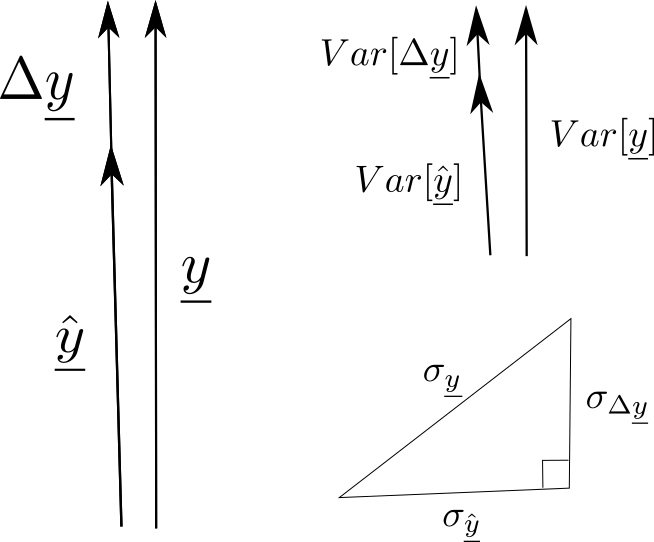
\includegraphics[width=2.3in]
{conventions/ms-error.png}
\caption{$\rvy=\HAT{y}+\Delta y$
and the variances (not standard deviations)
of these quantities add. }
\label{fig-ms-error}
\end{figure}

\section{Cramer-Rao Bound}

This discussion of the Cramer-Rao (CR) bound
is based on Ref.\cite{wiki-cramer-rao}.

Suppose $\rvx$ is a random variable with values $x\in S_\rvx$
and $\theta\in\RR$ is a parameter.
For any function
$f_{\rvx,\theta}: S_\rvx\times \RR\rarrow \RR$,
define

\beq
\av{f_{\rvx,\theta}} =\sum_x P(x|\theta)f_{x,\theta}
\eeq

\beq
\Delta f_{\rvx,\theta}=f_{\rvx,\theta}-\av{f_{\rvx,\theta}}
\eeq

\beq
\av{f_{\rvx,\theta},f_{\rvx,\theta}}=
\av{\Delta f_{\rvx,\theta}\;\Delta f_{\rvx,\theta}}
\eeq

Define the {\bf log likelihood function} by
\beq
LL_\theta = \ln P(x|\theta)
\eeq

Define the {\bf Fisher information} by
\beq
I_\theta=\av{\partial_\theta LL_\theta,\partial_\theta LL_\theta}
\eeq

Note that $LL_\theta\leq 0$.
Let $\theta^*$ be the
value of $\theta$ that maximizes $LL_\theta$.


Note that $I_\theta\geq 0$ and
$I_\theta=0$ when $\theta=\theta^*$
because $\partial_\theta LL_\theta|_{\theta=\theta^*}=0$.
This suggests that $I_\theta$
measures the distance
between $\theta$ and $\theta^*$.



Note that
\beqa
\av{\partial_\theta LL_\theta}&=&
\sum_x P(x|\theta)\frac{1}{P(x|\theta)}
\partial_\theta P(x|\theta)
\\
&=&
\partial_\theta \sum_x P(x|\theta)
\\
&=&
0
\eeqa
Therefore

\beqa
I_\theta &=&\av{[\partial_\theta LL_\theta]^2}
-
\av{\partial_\theta LL_\theta}^2
\\
&=&
\av{[\partial_\theta LL_\theta]^2}
\eeqa

\begin{claim}
\beq
I_\theta = -\av{\partial_\theta^2 LL_\theta}
\eeq
\end{claim}
\proof

\beqa
I_\theta &=& \av{[\partial_\theta LL_\theta]^2}
\\
&=&
\sum_x P(x|\theta)
\frac{1}{P(x|\theta)}
\partial_\theta P(x|\theta)
\partial_\theta \ln P(x|\theta)
\\
&=&
-\sum_x P(x|\theta)\partial_\theta^2 \ln P(x|\theta)
+ \partial_\theta\sum_x
P(x|\theta)\partial_\theta \ln P(x|\theta)
\\
&=&
-\av{\partial_\theta^2 LL_\theta}
+ \partial_\theta^2\sum_x P(x|\theta)
\\
&=&
-\av{\partial_\theta^2 LL_\theta}
\eeqa
\qed

\begin{claim}
If $x=[x_i]_{i=1,2, \ldots \nu}\in \RR^\nu$ are i.i.d., then


\beq
I_\theta = \nu \av{[\partial_\theta LL_{\theta, i}]^2}
\eeq
where

\beq
LL_{\theta, i} = \ln P(x_i|\theta)
\eeq
\end{claim}
\proof

\beqa
LL_\theta
&=& \ln \prod_i P(x_i|\theta)
\\
&=&
\sum_i LL_{\theta, i}
\eeqa

\beqa
I_\theta &=&
\sum_i \sum_j \av{
\partial_\theta LL_{\theta,i}
\partial_\theta LL_{\theta,j}
}
\\
&=&
\sum_i  \av{
[\partial_\theta LL_{\theta,i}]^2}
\\
&=&
\nu \av{
[\partial_\theta LL_{\theta,i}]^2
}
\eeqa
\qed




A function  $t_\rvx:S_\rvx\rarrow \RR$
is called a {\bf test statistic} of random variable $\rvx$.

\begin{claim}(Cramer-Rao bound for single parameter $\theta\in\RR$)

\beq
\av{t_\rvx,t_\rvx}I_\theta \geq
 \left[\partial_\theta\av{t_\rvx}\right]^2
 \label{eq-crao-tx}
 \eeq
\end{claim}
\proof

Cauchy-Schwartz inequality

For two vectors $\veca,\vecb\in\RR^n$:
\beq
\veca\cdot\vecb =|\veca||\vecb|\cos \phi \leq |\veca||\vecb|
\eeq

For two real valued random variables $\rva, \rvb$:
\beq
\av{\rva, \rva} \av{\rvb,\rvb}\geq |\av{\rva,\rvb}|^2
\eeq
Replace

\beq
\rva\rarrow t_\rvx,
\quad\rvb\rarrow \partial_\theta LL_\theta
\eeq
Then

\beqa
\av{t_\rvx, \partial_\theta LL_\theta}
&=&
\av{t_\rvx \partial_\theta LL_\theta}
-
\av{t_\rvx} \underbrace{\av{\partial_\theta LL_\theta}}_{=0}
\\
&=&
\sum_x P(x|\theta)
t_\rvx \frac{1}{P(x|\theta)}\partial_\theta P(x|\theta)
\\
&=&
\partial_\theta\sum_x  t_\rvx P(x|\theta)
\\
&=&
\partial_\theta\av{ t_\rvx}
\eeqa
\qed

See Fig.\ref{fig-cramer-rao}
for a pictorial representation
of Eq.(\ref{eq-crao-tx}).

\begin{figure}[h!]
\centering
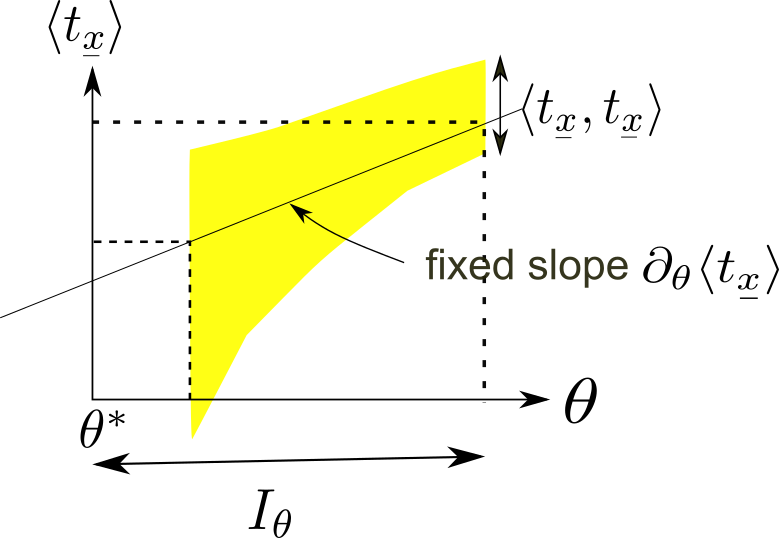
\includegraphics[width=2.7in]
{conventions/cramer-rao.png}
\caption{
In this drawing,
$\theta^*$ is the
value of $\theta$ that maximizes $LL_\theta$.
According
to the CR bound,
the product of the
variance $\av{t_\rvx, t_\rvx}$ and
the distance $I_\theta$
must be greater or equal to $[\partial_\theta\av{t_\rvx}]^2$.
At fixed $[\partial_\theta\av{t_\rvx}]^2$,
if the variance increases, the distance decreases,
and vice versa.
}
\label{fig-cramer-rao}
\end{figure}


Now suppose the test statistic $t_\rvx$
equals an {\bf estimator} $\HAT{\theta}$
of $\theta$ with bias $b_\rvx:S_\rvx \rarrow \RR$.

\beq
t_\rvx = \HAT{\theta}(\rvx) = \theta + b_\rvx
\eeq
$\HAT{\theta}$ is said to be a {\bf biased estimator}
if $b_\rvx\neq 0$ and an {\bf unbiased estimator} if $b_\rvx=0$.

\begin{claim}

\beq
\av{\HAT{\theta}} = \theta + \av{b_\rvx}
\eeq

\beq
\av{\HAT{\theta}, \HAT{\theta}} \geq
\frac{[1 + \partial_\theta\av{b_\rvx}]^2}
{I_\theta}
\label{eq-crao-theta}
\eeq

\beq
\av{[\HAT{\theta}-\theta]^2} \geq
\frac{[1 + \partial_\theta\av{b_\rvx}]^2}
{I_\theta}
+
\av{b_\rvx}^2
\eeq

\end{claim}
\proof
\beqa
\partial_\theta\av{t_\rvx}
&=&
\partial_\theta\av{\theta + b_\rvx}
\\
&=&
\partial_\theta\left[\theta +\av{b_\rvx}\right]
\\
&=&
1 + \partial_\theta\av{b_\rvx}
\eeqa
Eq.(\ref{eq-crao-theta})
follows from Eq.(\ref{eq-crao-tx})
once we replace $t_\rvx$ by $\HAT{\theta}$.

Let
\beq
\Delta \HAT{\theta} =
\HAT{\theta} -\av{\HAT{\theta}}
=
\underbrace{(\HAT{\theta} -\theta)}_\xi  - \av{b_\rvx}
\eeq
Then

\beq
0=\av{\Delta \HAT{\theta}} = \av{\xi} - \av{b_\rvx}
\eeq

\beqa
\frac{[1 + \partial_\theta\av{b_\rvx}]^2}
{I_\theta} &\leq&
\av{[\Delta \HAT{\theta}]^2}
\\
&=&
\av{\xi^2 -2\xi\av{b_\rvx} + \av{b_\rvx}^2}
\\
&=&
\av{\xi^2} -\av{b_\rvx}^2
\eeqa

\qed

Multi-dimensional case:
parameter
 $\theta=[\theta_1, \theta_2, \ldots, \theta_n]^T\in \RR^n$
 and test statistic
 $t_\rvx=[t_{\rvx,1}, t_{\rvx,2}, \ldots, t_{\rvx,n}]^T\in \RR^n$
are column vectors.

Define {\bf Fisher information matrix} by

\beq
[I_\theta]_{i,j}=
\av{\partial_{\theta_i} LL_\theta, \partial_{\theta_j}LL_\theta}
=
\av{\partial_{\theta_i} LL_\theta\;\partial_{\theta_j}LL_\theta}
\eeq

CR bound for multi-dimensional parameter $\theta\in\RR^n$:
\beq
\text{matrix}\left[\av{t_{\rvx,i}, t_{\rvx,j}}\right]\geq
\text{matrix}\left[
\partial_{\theta_i} \av{t_{\rvx,a}}
[I_\theta]^{-1}_{a,b}
\partial_{\theta_j} \av{t_{\rvx,b}}
\right]
\eeq
where we are using the Einstein summation
convention (repeated indices are summed over).
For two matrices $A,B\in\RR^n$, $A\geq B$ means $A-B$ has
non-negative eigenvalues.


\section{Bayes Rule,
Bayesian Updating And Conjugate Priors}

Bayes Rule says:

\beq
P(\theta|x)P(x)
=
P(x|\theta)P(\theta)
\eeq
Expressed diagramatically\footnote{Two bnets are equated if their full probability
distributions (i.e.,
their full instantiations) are equal numerically.
For example,  
$$
\rva\rarrow\rvb\rarrow \rvc = P(c|b)P(b|a)P(a)= \rva\larrow\rvb\larrow\rvc
$$},
we have for  $\rvx\in\RR$:
\beq
\xymatrix{
\rvtheta&\rvx\ar[l]
}
\quad =\quad
\xymatrix{
 \rvtheta\ar[r]&\rvx
}
\eeq
and for $\rvx=(\rvx_1, \rvx_2)\in \RR^2$:
\beq
\begin{array}{c}
\xymatrix@R=.3pc{
&\rvx_1\ar[ld]\ar[dd]
\\
\rvtheta
\\
&\rvx_2\ar[lu]
}
\xymatrix@R=.3pc{\\\quad =\quad}
\xymatrix@R=.3pc{
&\rvx_1\ar[dd]
\\
\rvtheta\ar[ru]\ar[rd]
\\
&\rvx_2
}
\end{array}
\eeq
Note how Bayes rule
allows us to reverse the
direction of the arrows
impinging on $\theta$.
We see from Bayes Rule
that even though
the directions of
the arrows in a
bnet can have causal
motivation, a bnet
with arrows reversed
from their causally
motivated directions
can still be very useful
as a calculation tool.

Another way of stating
Bayes Rule is




\beq
\underbrace{P(\theta|x)}_{\rm posterior}=
\caln(!\theta)
\underbrace{P(x|\theta)}_{\rm likelihood}
\underbrace{P(\theta)}_{\rm prior}
\;.
\eeq

If, for a given likelihood,
the prior and posterior
distributions belong to
the same family (for instance,
they are both
Beta distributions),
then we say that the prior is the
{\bf conjugate prior}
of that likelihood.

For example,
Beta $\sim$ Bernoulli*Beta.
Hence, the
Beta distribution\footnote{See
Ref.\cite{wiki-beta-dist} for a discussion
of the Beta distribution.}
is the conjugate prior of the
Bernoulli distribution\footnote{See
Ref.\cite{wiki-bern-dist} for a discussion
of the Bernoulli distribution}.
More explicitly,
if

\beq
p_1\sim {\rm Beta}(p_1;\alp, \beta)
\eeq
and

\beq
x|p_1\sim {\rm Bernoulli}(x;p_1)
\;,
\eeq
where $p_1=P(x=1)$,
then

\beq
p_1|x\sim {\rm Beta}(p_1;\alp', \beta')
\eeq
where

\beq
\alp'= \alp + x
\eeq

\beq
\beta'= \beta + (1-x)
\eeq


Ref.\cite{wiki-conj-prior}
has a table of
conjugate priors.

Conjugate priors facilitate
Bayesian updating
of the prior to
posterior in a
feedback loop(see Fig.\ref{fig-conj-prior}).

\begin{figure}[h!]
$$\xymatrix{
&x_t\ar[d]
\\
&\stackrel{Bernoulli}{P(x_t|\theta)}\ar@/_2pc/[ld]
\\
\stackrel{Beta}{P(\theta|x_{\leq t})}\ar@/_2pc/[rd]
&&\stackrel{Beta}{P(\theta|x_{\leq t-1})}\ar@/_2pc/[ul]
\\
&t\rarrow t+1 \text{ for } t=0, 1, 2,\ldots
\ar@/_2pc/[ur]
}$$
\caption{Bayesian updating facilitated
by conjugate prior. In this figure,
$x_{\leq t}=(x_0, x_1, \ldots, x_{t-1}, x_t)$.}
\label{fig-conj-prior}
\end{figure}


\section{Linear regression, Ordinary Least Squares (OLS)}
\label{sec0-conv-lr}
Wikipedia articles
\begin{enumerate}
\item
Linear Regression (LR)
\begin{itemize}
\item
linear regression, Ref.\cite{wiki-lr}
\item
 simple linear regression, Ref.\cite{wiki-slr}
\item
errors in variable, Ref.\cite{wiki-errors-in-iv}

\end{itemize}
\item
Least squares (LS)
\begin{itemize}
\item
least squares, Ref.\cite{wiki-lsquares}
\item
ordinary least squares (OLS), Ref.\cite{wiki-ols}
\end{itemize}
\end{enumerate}


Some nomenclature: In LR, the
data consists of
{\bf independent x-variables} $x^\s_1,
 x^\s_2, \ldots x^\s_n$
and a {\bf dependent y-variable} $y^\s$.
We find a linear fit $\haty^\s =
\beta_0 + \sum_{i=1}^n \beta_i x^\s_i$
to the data.
$\haty^\s$ is called the {\bf estimate}
of $y^\s$.
 The coefficients $\beta_0, \beta_i$
are called {\bf regression coefficients}.
$y^\s-\haty^\s=\eps^\s$
are called  the {\bf residuals}.
$\cale =\sum_\s (\eps^\s)^2$
is called the {\bf error or cost}. We choose the
regression coefficients
so as to minimize the error.

Below, we consider two types of LR:

\begin{enumerate}
\item
LR
in which the independent x-variables are non-random.
\item
LR
in which the independent x-variables are random
and i.i.d.
\end{enumerate}

The  term OLS
is often used to refer to LR
of type 1.



For LR of type 2,
there is randomness in $y$
coming from the randomness in $x$
and in the residuals.
For LR of type 1,
there  is randomness in $y$
too, but
it comes
from the residuals
only.

Once one assumes that certain
variables are random, a
``model" (i.e., a bnet,
with probabilities expressed as TPMs)
 must be
specified.


\subsection{LR, assuming
$x_\s$ are non-random}

Let

$\s\in\{0, 1, 2, \ldots, nsam-1\}$ : sample index

$i_0\in\{0, 1, 2, \ldots, n\}$ :
index that can assume values 0 to $n$

$i\in\{1, 2, \ldots, n\}$ :
index that can assume values 1 to $n$.
$i$ is never equal to 0.


$y_\s\in \RR$: dependent y-variables

$x_{\s i}\in \RR$: independent x-variables

$\eps_\s\in \RR$: residuals

$\beta_0, \beta_i\in \RR$:
regression coefficients


\beq
y_\s= \beta_0 +
\sum_{i=1}^{n} x_{\s i}\beta_{i} + \eps_\s
\label{eq-LR-start}
\eeq

If we define
\beq
x_{\s 0}=1
\;
\eeq
for all $\s$, then

\beq
y_\s=
\sum_{i_0=0}^{n} x_{\s i_0}\beta_{i_0} + \eps_\s
\;.
\eeq
If $y$ and $\eps$ are $nsam$ dimensional
 column vectors and $\beta$
is an $n+1$ dimensional column vector,
and $X$ is an $nsam\times (n+1)$ matrix,
then we can write the previous equation in matrix
form as:


\beq
y=X\beta+\eps
\;.
\eeq

\subsubsection{Derivation of LR
 From Minimization of Error}

Let $W=[W_{\s, \s'}]$
be a symmetric matrix with non-negative
diagonal elements $W_{\s,\s}\geq 0$ for all $\s$.
$W$ is called the {\bf weight matrix}.
The following claim
describes the method of
{\bf Weighted LR}
when $W\neq 1$
and of simple LR  when $W=1$.
\begin{claim}
Assume the
Einstein summation convention; i.e.,
implicit sum over
repeated indices.
The
 error function $\cale$ given by

\beq
\cale=
\underbrace{(y_{\s}-X_{\s, j_0}\beta_{j_0})}
_{\text{residual $\eps_\s$}}
W_{\s, \s'}
\underbrace{(y_{\s'}-X_{\s', k_0}
\beta_{k_0})}_{\eps_{\s'}}
\;,
\eeq
is minimized
over $\beta_{k_0}$ for all $k_0
\in\{0,1,\ldots,n\}$,
if $\beta_{k_0}$ is given by:

\beq
\HAT{\beta}= (X^T W X)^{-1} X^T W y
\;.
\label{eq-betahat-non-ran-w}
\eeq
When $W=1$,

\beq
\HAT{\beta}= (X^T X)^{-1} X^T y
\;.
\label{eq-betahat-non-ran}
\eeq

\end{claim}
\proof

At the minimum of $\cale$,
the variation $\delta\cale$
 must vanish:
\beq
0=\delta \cale=
-2 X_{\s j_0}(\delta \beta_{j_0})
W_{\s, \s'}(y_{\s'}
-X_{\s' k_0}
\beta_{k_0})
\;.
\eeq
Thus,

\beq
X^T W y - X^T W X\beta=0
\eeq
which
implies Eq.(\ref{eq-betahat-non-ran-w}).
\qed

\subsubsection{Geometry of LR
with non-random $x_\s$.}

Recall that

\beq
y=X\beta+\eps
\;.
\eeq


Define the {\bf projection matrices}

\beq
\A=X(X^TX)^{-1}X^T
\;,\;\;\V=1-\A
\eeq
A square matrix $M$
is symmetric if $M^T=M$
and is idempotent if $M^2=M$.
$\A$ is symmetric
and idempotent
and so is $\V$.
Note that $\A$ and $\V$
also satisfy:

\beq
\V\A=\A\V=0
\eeq
and

\beq
\A X=X\;,\;\; \V X=0
\;.
\eeq

One has

\beq
\beta=
(X^TX)^{-1}X^T(y-\eps)
\;.
\eeq


Define

\begin{subequations}
\beq \boxed{
\HAT{\beta}=
\underbrace{(X^TX)^{-1}X^T}_B \;y
\;,
}
\label{eq-beta-nonrandom-lin-reg}
\eeq



\beq
\HAT{y}=
X\HAT{\beta}= \A y
\;,
\eeq
and

\beq
\HAT{\eps}=
y-X\HAT{\beta}=
y-\HAT{y}=(1-\A)y=\V y
\;.
\eeq
\end{subequations}
$\A$ is sometimes  called the {\bf hat matrix},
because it gives $y$ a hat.

Given any function $f=f(y,X,\eps)$
and a scalar factor $\xi\in \RR$,
suppose
$f(\xi y, \xi X, \xi\eps)=\xi^\calo f(y,X,\eps)$.
Then we will say that $f(\cdot)$
is of {\bf order $\calo$ under scaling}.
Note that $\{\HAT{y},
 \HAT{\eps}\}$
are all of order 1 under scaling,
$\{\beta, \HAT{\beta}, \A, \V\}$
are all of order 0 under scaling,
and $B$ is of order $-1$ under scaling.
Thus, each cfit (i.e., symbol
with a hat)
scales the same way as its estimand (i.e., same
symbol
without a hat). Furthermore,
$\beta$, its cfit $\HAT{\beta}$, and
the projection matrices $\A, \V$
are invariant ($\calo=0$) under scaling.



Note that $y$
can be expressed as
a sum of 2 orthogonal estimates:



\beq
y= \underbrace{\HAT{y}}_{\A y} +
\underbrace{\HAT{\eps}}_{\V y}
\;.
\eeq
Fig.\ref{fig-lin-reg-vecs}
shows triangles representing
$y=X\beta+\eps$ and $y=\HAT{y}+\HAT{\eps}$.


\begin{figure}[h!]
\centering
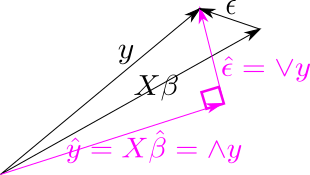
\includegraphics[width=2in]
{conventions/lin-reg-vecs.png}
\caption{Triangles
representing
$y=X\beta+\eps$ and $y=\HAT{y}+\HAT{\eps}$.}
\label{fig-lin-reg-vecs}
\end{figure}

\subsubsection{LR Goodness of Fit, $R^2$}


Assume the components of $\eps$
are random with zero mean:

\beq
E[\rveps]=\av{\rveps}=0
\eeq



Assume $X$ and $\beta$ are not random.
This makes $\rvy=X\beta +\rveps$ and $\ul{\HAT{\beta}}=
(X^TX)^{-1}X^T\rvy
$
random.
One finds that

\begin{subequations}
\beq
\av{\rvy}=X\beta
\eeq


\beq
\av{\HAT{\rvy}}=\A
\underbrace{\av{\rvy}}_{X\beta}
=\av{\rvy}
\eeq

\beq
\av{\HAT{\rveps}}=\V
\underbrace{\av{\rvy}}_{X\beta}
=0
\eeq

\beq
\av{\ul{\HAT{\beta}}}=\beta
\eeq


So far, we have
assumed a zero mean value for $\eps$.
Next, assume
{\bf  ``homoscedasticity" (homo-spread)}\footnote{I
 find the word ``homoscedasticity"
unnecessarily long, cryptic
and easy to misspell so
I like to replace
it by ``homo-spread".
The opposite
of ``homoscedasticity"
is ``heteroscedasticity",
which I like to replace with ``hetero-spread".}, which
means that

\beq
\av{\rveps, \rveps^T}=\xi^2 I_{nsam}
\eeq
\end{subequations}
where
$\xi\geq 0$,  and
$I_{nsam}$ is the
$nsam\times nsam$ identity matrix.
It follows that

\begin{subequations}
\label{eq-lin-re-variances}
\beq
\av{\rvy, \rvy^T}=
\av{\rveps, \rveps^T}=
\xi^2 I_{nsam}
\;,
\eeq

\beq
\av{\HAT{\rveps},
\HAT{\rveps}^T}=
\V\av{\rvy, \rvy^T}\V^T=\xi^2\V
\label{eq-homo}
\;,
\eeq

\beq
\av{\HAT{\rvy},
\HAT{\rvy}^T}=
\A\av{\rvy, \rvy^T}\A^T=\xi^2\A
\eeq
and

\beq
\av{\HAT{\ul{\beta}},
\HAT{\ul{\beta}}^T}=
B\av{\rvy, \rvy^T}B^T=\xi^2 (X^TX)^{-1}
\;.
\eeq
\end{subequations}

For any random column vector $\rva$,
let

\beq
\norm{\rva}^2= \rva^T\rva=\tr(\rva\rva^T)
\eeq
and

\beq
\av{\norm{\rva-\av{\rva}}^2}=
\av{\rva^T\rva}-\av{\rva^T}\av{\rva}
=
\tr\av{\rva, \rva^T}
\;.
\eeq

Define the following sums of squares (SS):

\begin{subequations}
\label{eq-lin-reg-ss}
\beq
SS_{\rvy}=\av{\norm{\rvy-\av{\rvy}}^2}
=\av{\rvy^T\rvy}-\av{\rvy^T}\av{\rvy}
=\tr\av{\rvy,\rvy^T}
\eeq

\beq
SS_{\HAT{\rvy}}=\av{\norm{\HAT{\rvy}-\av{\HAT{\rvy}}}^2}
=\av{\HAT{\rvy}^T\HAT{\rvy}}-\av{\HAT{\rvy}^T}\av{\HAT{\rvy}}
=\tr\av{\HAT{\rvy},\HAT{\rvy}^T}
\eeq

\beq
SS_{res}=\av{\norm{\rvy-\HAT{\rvy}}^2}
=
\av{\norm{\ul{\HAT{\eps}}}^2}
=\tr\av{\ul{\HAT{\eps}},\ul{\HAT{\eps}}^T}
\eeq
\end{subequations}

\begin{claim}
The following is true
without homo-spread:


\beq
\underbrace{\tr\av{\rvy,\rvy^T} }_{SS_\rvy}
=
\underbrace{\tr\av{\HAT{\rvy}, \HAT{\rvy}^T}}_{SS_{\HAT{\rvy}}}
+
\underbrace{\tr\av{\HAT{\rveps}, \HAT{\rveps}^T}}_{SS_{res}}
\eeq
This is like the Pythagorean Theorem
for the magenta right triangle
in Fig.\ref{fig-lin-reg-vecs}.
\end{claim}
\proof

From Eqs.\ref{eq-lin-re-variances}
and \ref{eq-lin-reg-ss},
we see that

\beq
SS_\rvy=\tr\av{\rvy,\rvy^T}
\eeq

\beq
SS_{\HAT{\rvy}}=\tr\av{\HAT{\rvy},\HAT{\rvy}^T}
=\tr\av{\A\rvy, \rvy^T}
\eeq

\beq
SS_{res}=\tr\av{\HAT{\rveps}, \HAT{\rveps}^T}
=\tr\av{\V\rvy, \rvy^T}
\eeq
Now use $\A + \V=1$.
\qed


The goodness of fit
for this model
is often measured using  the
{\bf coefficient of determination}
$R^2$. $R^2$  is defined by


\beq
R^2= 1 -\;\frac{SS_{res}}{SS_\rvy}=
\frac{SS_{\HAT{y}}}{SS_\rvy}
=
\frac{\tr \av{\HAT{\rvy},\HAT{\rvy}^T}}
{ \tr \av{\rvy,\rvy^T}}
\eeq
If homo-spread holds, then
$R^2$ reduces to


\beq
R^2 =\frac{\tr\; \A}{nsam}
\;.
\eeq


\subsection{LR, assuming
$x_\s$ are random}
Let

$i_0\in\{0, 1, 2, \ldots, n\}$ :
index that can assume values 0 to $n$

$i\in\{1, 2, \ldots, n\}$ :
index that can assume values 1 to $n$.
$i$ is never equal to 0.


$\rvy\in\RR$:  true value
of dependent y-variable

$\HAT{\rvy}\in\RR$: cfit
of dependent y-variable

$\ul{\eps}\in\RR$: residual



$\rvx_{i}\in \RR$: independent x-variables
for $i\in\{1,\ldots,n\}$

$\beta_0, \beta_i\in\RR$:
regression coefficients

\beqa
\HAT{\rvy}
&=&
\beta_0 +\sum_{j=1}^{n}
\beta_{j} \rvx_j
\\
&=&
\sum_{j_0=0}^{n}\beta_{j_0} \rvx_{j_0}
\;\;(\text{Assume $\rvx_0=1$.})
\eeqa

\beq
\rvy = \HAT{\rvy}+\ul{\eps}
\eeq

\subsubsection{Transforming
expressions
from
non-random to
random $x_\s$ }

Define the following
population averages:


\beq
E_\s[x^\s]=
\frac{1}{nsam}
\sum_\s x^\s
\;,
\eeq

\beq
E_\s[x^\s y^\s]=
\frac{1}{nsam}
\sum_\s x^\s y^\s
\;,
\eeq

\beq
\av{x^\s,y^\s}_\s=
E_\s[x^\s y^\s]-E_\s[x^\s]E_\s[y^\s]
\;.
\eeq


\begin{claim}\label{cl-sigma-to-ran}
If the $x_\s$ are i.i.d. random
variables,

\beq
E_\s[x^\s] =\av{\rvx}
\;
\label{eq-exp-x}
\eeq
\beq
E_\s[x^\s y^\s]
=
\av{\rvx\rvy}
\label{eq-exp-xy}
\eeq

\beq
\av{x^\s,y^\s}_\s
=
\av{\rvx, \rvy}
\label{eq-exp-x--y}
\eeq
\end{claim}
\proof
\beqa
\frac{1}{nsam}
\sum_\s x^\s
&=&
\frac{1}{nsam}
\sum_{x\in S_\rvx}
x
\underbrace{
\sum_\s \indi(x^\s=x)}_
{N(x^\s=x)}
\\
&=&
\sum_{x}x\;P(x)
\\
&=&
\av{\rvx }
\eeqa

\beqa
\frac{1}{nsam}
\sum_\s x^\s y^\s
&=&
\frac{1}{nsam}
\sum_{x\in S_\rvx}
\sum_{y\in S_\rvy}
xy
\underbrace{
\sum_\s \indi(x^\s=x, y^\s=y)}_
{N(x^\s=x, y^\s=y)}
\\
&=&
\sum_{x,y}xy\;P(x,y)
\\
&=&
\av{\rvx \rvy}
\eeqa
Eq.(\ref{eq-exp-x--y})
follows from
Eq.(\ref{eq-exp-x}) and Eq.(\ref{eq-exp-xy}).
\qed

Recall that

\beq
Y_\s = \beta_0 +  \sum_{j=1}^n X_{\s,j}\beta_j + \eps_\s
\;.
\eeq

Assume
\beq
E_\s[X_{\s,k} \eps_\s]=E_\s[X_{\s,k}]
\underbrace{E_\s[ \eps_\s]}_{=0}=0
\;.
\eeq
Then we have

\beq
E_\s[X_{\s,k} Y_\s]=
E_\s[X_{\s,k}]\beta_0 + \sum_{j=1}^n
E_\s [X_{\s,k} X_{\s,j}] \beta_j +
\underbrace{E_\s[X_{\s,k} \eps_\s]}_{=0}
\label{eq-EXY}
\eeq
and

\beq
E_{\s'}[X_{\s',k}]E_\s[ Y_\s]=
E_{\s'}[X_{\s',k}]\beta_0 + \sum_{j=1}^n
E_{\s'} [X_{\s',k}] E_\s[ X_{\s,j}] \beta_j +
\underbrace{E_{\s'}[X_{\s',k}]  E_\s[ \eps_\s]}_{=0}
\label{eq-EX-EY}
\;.
\eeq
Subtracting
Eq.(\ref{eq-EX-EY}) from Eq.(\ref{eq-EXY}), we get

\beq
\av{X_{\s,k} ,Y_\s}_\s=
\sum_{j=1}^n
\av{X_{\s,k}, X_{\s,j}}_\s \beta_j
\label{eq-avX-comma-Y}
\;.
\eeq
Define the $n$ dimensional
covariance matrix $C$
by

\beq
C_{k,j}=\av{X_{\s,k}, X_{\s,j}}_\s
\:.
\eeq
Then Eq.(\ref{eq-avX-comma-Y}) implies

\beq
\beta_j =\sum_{k=1}^n
C^{-1}_{j,k} \av{X_{\s,k} ,Y_\s}_\s
\label{eq-beta_j-c-inv}
\eeq
for all $j=1,2,\ldots, n$.

If we assume that the $x_\s$ are i.i.d.,
then, by  virtue of Claim \ref{cl-sigma-to-ran},
the matrix $C$ tends to


\beq
C_{k,j}
\rarrow \av{\rvx_k, \rvx_j}
\eeq
and Eq.(\ref{eq-beta_j-c-inv})
implies

\beq
\beta_j = \sum_{k=1}^n C^{-1}_{j,k}\av{\rvx_k, \rvy}
\label{eq-beta-random-from-nonrandom}
\;.
\eeq

\subsubsection{Geometry of LR with random $x_\s$}
Recall that

\beq
\rvy =
\underbrace{\beta_0 +\sum_{j=1}^{n}
\beta_{j} \rvx_j}_{\HAT{\rvy}}
+\ul{\eps}
\;.
\eeq


Assume

\beq
\av{\rveps}=0
\eeq
and
\beq
\av{\rvx_j, \ul{\eps}}=0
\eeq
for all $j$.

For $k=1, \ldots, n$,
\beq
\av{\rvx_k, \rvy}
=
\sum_{j=1}^{n}\beta_j\av{\rvx_k, \rvx_j}
\;.
\label{eq-beta-0-wrong}
\eeq

Let $\rvx^n$ and $\beta^n$ be
$n$-dimensional column vectors.
Then Eq.(\ref{eq-beta-0-wrong})
can be represented
 in matrix notation by
\beq
\av{\rvx^n, \rvy}=
\av{\rvx^n, (\rvx^n)^T}\beta^n
\;.
\eeq
Hence,

\beq
\boxed{
\beta^n=
\av{\rvx^n, (\rvx^n)^T}^{-1}
\av{ \rvx^n, \rvy}
\;.}
\label{eq-beta-random-lin-reg}
\eeq
For $\beta_0$, use

\beq
\beta_0=
\av{\rvy}-\av{\rvx^n}^T \beta^n
\eeq

Notice that
Eq.(\ref{eq-beta-random-lin-reg})
for the regression coefficients
is the same
as Eq.(\ref{eq-beta-random-from-nonrandom}).
So we have rederived the same formula
via a different method.


Next, we will
write
 Eq.(\ref{eq-beta-random-lin-reg})
for the special cases
$n=1$ and $n=2$,
where $n$ is the
number of independent x-variables $\rvx_j$

\begin{enumerate}
\item $n=1$ ($\rvy$ fitted by a line)

\beq
\rvy = \beta_0 + \beta_1\rvx + \rveps
\eeq

Eq.(\ref{eq-beta-random-lin-reg}) becomes
\beq
\beta_1=
\frac{\av{\rvy,\rvx}}{\av{\rvx,\rvx}}
\eeq


\item $n=2$ ($\rvy$ fitted by a plane)


\beq
\rvy = \beta_0 + \beta_1 \rvx_1 + \beta_2 \rvx_2 +\rveps
\eeq
Define


\beq
C_{i,j}=\av{\rvx_i, \rvx_j}
\eeq
for all $i,j$.
Then Eq.(\ref{eq-beta-random-lin-reg})
becomes\footnote{
Recall that if
$
M=
\left[
\begin{array}{cc}
a&b
\\
c&d
\end{array}
\right]
$
then
$
M^{-1}
=
\frac{1}{\det M}
\left[
\begin{array}{cc}
d&-b
\\
-c&a
\end{array}
\right]
$
}


\beqa
\left[
\begin{array}{c}
\beta_1
\\
\beta_2
\end{array}
\right]
&=&
C^{-1}
\left[
\begin{array}{c}
\av{\rvy, \rvx_1}
\\
\av{\rvy, \rvx_2}
\end{array}
\right]
\\
&=&
\frac{1}{\det C}
\left[
\begin{array}{cc}
C_{22}&-C_{12}
\\
-C_{21}&C_{11}
\end{array}
\right]
\left[
\begin{array}{c}
\av{\rvy, \rvx_1}
\\
\av{\rvy, \rvx_2}
\end{array}
\right]
\eeqa


Hence,
\beq
\beta_1
=\pder{\rvy}{\rvx_1}=
\frac{
C_{22}\av{\rvy, \rvx_1}
-C_{12}\av{\rvy, \rvx_2}
}
{
C_{11}C_{22}-C_{12}^2
}
\label{eq-beta-lr-plane}
\eeq
Eq.(\ref{eq-beta-lr-plane})
 agrees with
the
value of $\beta_{YX, Z}$ in
Ref.\cite{pearl-lin-reg}
by Pearl,
if  we replace in Pearl's
formulae $X\rarrow \rvx_1$,
$Y\rarrow \rvy$, $Z\rarrow \rvx_2$.


\end{enumerate}

\subsubsection{Regression
 interpreted as differentiation
 of $y$}

Finding the derivative of $y$
with respect to (wrt) $X$
(a.k.a. ``{\bf Regressing $y$ on $X$}")
is finding
$\HAT{\beta}=\frac{d}{dX}
\underbrace{y}_{X\beta}$.

Recall that

\beq
\rvy = \beta_0 + \sum_{k=1}^n \rvx_k \beta_k + \ul{\eps}
\;.
\eeq
Therefore,

\beqa
\av{\rvx_i, \rvy}
&=&
\sum_{k=1}^n \av{\rvx_i, \rvx_k}\beta_k
\\
&=&
 \av{\rvx_i, \rvx_i}\beta_i
+
\sum_{k=1}^n
\indi(k\neq i)
 \av{\rvx_i, \rvx_k}\beta_k
\;.
\eeqa
Hence,

\beq
\beta_i
=
\frac{\av{\rvx_i, \rvy}}
{\av{\rvx_i, \rvx_i}}
-\sum_{k=1}^n
\indi(k\neq i)
\frac{ \av{\rvx_i, \rvx_k}}
{\av{\rvx_i, \rvx_i}}
\beta_k
\;.
\label{eq-beta-i-non-deriv}
\eeq

Let's represent
the linear
operator
$\av{\rvx_i, \rvx_i}^{-1}\av{\rvx_i, \cdot}
$ as a derivative:

\beq
\frac{d\;\cdot}{d\rvx_i}=
\frac{\av{\rvx_i, \cdot}}
{\av{\rvx_i, \rvx_i}}
\;.
\eeq
Eq.(\ref{eq-beta-i-non-deriv})
can be expressed
in derivative notation as:

\beq
\beta_i
=
\frac{d \rvy}
{d\rvx_i}
-\sum_{k=1}^n\indi(k\neq i)
\frac{ d\rvx_k}
{d\rvx_i}
\beta_k
\label{eq-beta-i-deriv}
\eeq
Note that Eq.(\ref{eq-beta-i-deriv})
evokes the formula for differentials:

\beq
d\rvy=
\sum_{k=1}^n \beta_kd\rvx_k
\;.
\eeq

Note also that,
because of the
linearity of the derivative operator,
Eq.(\ref{eq-beta-i-deriv})
implies:

\beq
\beta_i=
\frac{d}
{d\rvx_i}
\left(\rvy
-
\underbrace{\sum_{k=1}^n
\indi(k\neq i)\rvx_k \beta_k
}_{\rvy-\rvx_i\beta_i}
\right)
\label{eq-beta-i-2-steps}
\;.
\eeq

Eq.(\ref{eq-beta-i-2-steps})
can be used to find
$\HAT{\beta}_i$
in two steps:

STEP 1: Regress $\rvy-\rvx_i\beta_i$
on $(\rvx_k)_{k\in \{1,2,
\ldots, n\}- \{ i\}}$.
Get estimates
$(\HAT{\beta}_k)_{k\in \{1,2,
\ldots, n\}- \{ i\}}$.

STEP 2: Regress $\rvy-\sum_{k\neq i} \rvx_k\HAT{\beta}_k$ on $\rvx_i$.
Get estimate $\HAT{\beta}_i$.

Of course, one can also
find $\HAT{\beta}_i$
by regressing $\rvy$
on $(\rvx_k)_{k\in \{1,2,
\ldots, n\}}$, to get
estimates
$(\HAT{\beta}_k)_{k\in \{1,2,
\ldots, n\}}$.

\section{Logistic Regression (LoR)}

Suppose
$x_\s\in \RR^n$,
$y_\s\in \RR$,
and $\Sigma$
is a population
of individuals $\s$.
In general,
a {\bf regression}
is when
we curve-fit a dataset
$\{(x_\s, y_\s):\s\in\Sigma\}$
with a function
$\haty=f(x)$.
In {\bf Linear
Regression (LR)},
which we
discussed earlier,
$f(x)$ is a hyperplane
in $x$.
On the other hand,
in {\bf Logistic Regression (LoR)},
$y_\s\in[0,1]$ and
$f(x)$ is the sigmoid of
a hyperplane in $x$.



More specifically, for LR
we have
Eq.(\ref{eq-LR-start})
which reads as follows:

\beq
y_\s=
\underbrace{
\beta_0 +
\sum_{i=1}^{n} x_{\s i}\beta_{i}
}_{\haty_\s}+ \eps_\s
\quad\text{(LR)}\;.
\eeq
For LoR, we have instead

\beq
p_\s=
\smoid\left(
\beta_0 +
\sum_{i=1}^{n} x_{\s i}\beta_{i} + \eps_\s
\right)
\quad\text{(LoR)}\;,
\eeq
or, equivalently,


\beq
\underbrace{\lodds(p_\s)}
_{\ln \frac{p_\s}{1-p_\s}}=
\underbrace{
\beta_0 +
\sum_{i=1}^{n} x_{\s i}\beta_{i}
}_{\haty_\s} + \eps_\s
\quad\text{(LoR)}\;,
\eeq
where we have used the fact that
$\lodds()$
is the inverse function of $\smoid()$.
Hence, an LoR
fit can be calculated by
collecting a dataset
$\{(x_\s, p_\s):\s\in\Sigma\}$,
transforming that
dataset to the dataset
$\{(x_\s,\lodds( p_\s)):\s\in\Sigma\}$,
and fitting the latter dataset
with a hyperplane.
Let $P(\rvY_\s=1)=p_\s\in [0,1]$.
LoR can be used
for binary
classification
if we define the
binary class
variable $c_\s\in \bool$ by

\beq
c_\s =\indi(P(\rvY_\s=1)>\alp)
\eeq
for some $0<\alp<1$.



\section{Entropy,
 Kullback-Leibler divergence, Cross-Entropy}

For probability distributions $p(x), q(x)$ of $x\in S_\rvx$
\begin{itemize}
\item
Entropy:
\beq
H(p)=-\sum_x p(x)\ln p(x)\geq 0
\eeq

\item
Kullback-Leibler divergence:

\beq
D_{KL}(p\parallel q)=\sum_{x} p(x)\ln \frac{p(x)}{q(x)}\geq 0
\eeq
\item
Cross entropy:
\beqa
CE(p\parallel q) &=& -\sum_x p(x)\ln q(x)\\
&=& H(p) + D_{KL}(p\parallel q)
\eeqa
\end{itemize}

\section{Definition of various
entropies used in Shannon Information Theory}

\begin{itemize}
\item
{\bf (plain) Entropy of $\rvx$}

\beq
H(\rvx) =
-\sum_{x} P(x)\ln P(x)
\eeq
This quantity measures the
spread of $P_\rvx$.
$H(\rvx)\geq 0$
and it vanishes iff $P(x)=\delta(x,x_0)$ (deterministic case)


\item
{\bf Conditional Entropy of $\rvy$ given $\rvx$}

\beqa
H(\rvy|\rvx) &=&
-\sum_{x,y}P(x,y)\ln {P(y|x)}
\\
&=&
H(\rvy,\rvx)-H(\rvx)
\eeqa
This quantity measures  the conditional
 spread
of $\rvy$ given $\rvx$. $H(\rvy|\rvx)\geq 0$.


\item {\bf Mutual Information (MI)
of $\rvx$ and $\rvy$}.

\beqa
H(\rvy:\rvx) &=&
\sum_{x,y} P(x,y) \ln \frac{P(x,y)}{P(x)P(y)}
\\
&=&
H(\rvx) + H(\rvy) - H(\rvy,\rvx)
\eeqa
This quantity measures the correlation
between $\rvx$ and $\rvy$.
$H(\rvy:\rvx)\geq 0$
and it vanishes iff
$P(x,y)=P(x)P(y)$.

\item {\bf Conditional Mutual Information
(CMI)\footnote{CMI
can be read as ``see me".}
of $\rvx$ and $\rvy$
given $\ul{\lam}$}


\beqa
H(\rvy:\rvx|\ul{\lam})
&=&
\sum_{x,y, \lam}P(x,y, \lam) \ln
\frac{P(x,y|\lam)}{P(x|\lam)P(y|\lam)}
\\
&=&
H(\rvx|\ul{\lam}) + H(\rvy|\ul{\lam})
- H(\rvy,\rvx|\ul{\lam})
\eeqa

This
quantity measures the conditional correlation
of $\rvx$ and $\rvy$ given $\ul{\lam}$.
$H(\rvy:\rvx|\ul{\lam})\geq 0$
and it vanishes iff
$P(x,y|\lam)=P(x|\lam)P(y|\lam)$.

An interesting special case
occurs when
$P(\lam)=\delta(\lam, \lam_0)$ (the
frequentist  case of no $\lam$ prior.)
In that case CMI
reduces to

\beq
H(\rvy:\rvx|\lam_0)
=
\sum_{x,y}P(x,y|\lam_0) \ln
\frac{P(x,y|\lam_0)}{P(x|\lam_0)P(y|\lam_0)}\geq 0
\eeq



\item {\bf Kullback-Leibler Divergence
from $P_\rvx$ to $P_\rvy$.}

Assume random variables $\rvx$
and $\rvy$
have the same set of states
$S_\rvx=S_\rvy$. Then


\beq
D_{KL}(P_\rvx\parallel P_\rvy)=
\sum_x P_\rvx(x) \ln \frac{P_\rvx(x)}{P_\rvy(x)}
\eeq

This quantity measures a non-symmetric distance
between the probability distributions
$P_\rvx$ and $P_\rvy$.
$D_{KL}(P_\rvx\parallel P_\rvy)\geq 0$
and it equals zero iff $P_\rvx=P_\rvy$.

\end{itemize}

\section{Mean log likelihood asymptotic behavior}
\label{sec-ent-like-connect}

Define the log likelihood  by
\beq
 LL_{y|\theta} = \ln P(y|\theta)
\;.
\eeq
In this section, we will represent averages over $\rvy|\theta$ by
angular brackets:
\beq
\av{f(y)}= \sum_y P(y|\theta) f(y)= E_{\rvy|\theta}[f(y)]
\;.
\eeq
Note that the mean log likelihood equals minus the entropy:

\beq
H(\rvy|\theta)= -\av{ LL_{y|\theta}}
\eeq

\begin{claim}

\beq
\av{\partial_\theta   LL_{y|\theta}}=0
\eeq

\beq
\av{\partial^2_\theta   LL_{y|\theta}}=
-\av{ (\partial_\theta  LL_{y|\theta})^2 }
\eeq

\end{claim}
\proof

\beqa
\av{\partial_\theta   LL_{y|\theta}}
&=&
\sum_y P(y|\theta)\partial_\theta\ln  P(y|\theta)
\\
&=&
\sum_y \partial_\theta P(y|\theta)
\\
&=& 0
\eeqa


\beqa
\av{\partial^2_\theta   LL_{y|\theta}}
&=&
\sum_y  P(y|\theta)\partial_\theta \left[ \frac{1}{P(y|\theta)}
 \partial_\theta P(y|\theta) \right]
\\
&=&
- \sum_y  P(y|\theta)
\frac{1}{P(y|\theta)^2}[ \partial_\theta P(y|\theta)]^2
+  \underbrace{ \sum_y   \partial_\theta^2   P(y|\theta)}_{=0}
\\
&=&
-\sum_y  P(y|\theta)[ \partial_\theta \ln P(y|\theta)]^2
\\
&=&
-\av{ (\partial_\theta  LL_{y|\theta})^2 }
\eeqa
\qed

Define
\beq
\Delta \theta =  \theta' - \theta
\eeq
and

\beq
-\Delta H(\rvy|\theta)=
\Delta\av{  LL_{y|\theta}}
=
\av{  LL_{y|\theta'}}-
\av{  LL_{y|\theta}}
\;
\eeq
If we expand
$\av{  LL_{y|\theta'}}$ as a Taylor series
to second order
about the point $\theta'=\theta$,
we get


\beq
\av{  LL_{y|\theta'}}=
\av{  LL_{y|\theta}}
+
\Delta \theta
\underbrace{\av{ \partial_\theta LL_{y|\theta}}}_{=0}
+
\frac{(\Delta\theta)^2}{2}
\underbrace{\av{ \partial^2_\theta LL_{y|\theta}}}_
{-\av{ (\partial_\theta LL_{y|\theta})^2} }
+ \calo((\Delta\theta)^3)
\eeq

\beq
-\Delta H(\rvy|\theta)=\Delta\av{  LL_{y|\theta}}
=
-\;\frac{(\Delta\theta)^2}{2}
\av{ (\partial_\theta LL_{y|\theta})^2}
+ \calo((\Delta\theta)^3)
\eeq
Thus, $\theta'=\theta$ maximizes
the mean log likelihood $\av{  LL_{y|\theta}}$
(and minimizes the entropy $H(\rvy|\theta)$).

Note that
\beq
\Delta\av{  LL_{y|\theta}}
=
\av{\ln \frac{P(y|\theta')}{P(y|\theta)}}
\;.
\eeq
If we approximate
the ratio of these 2 probabilities by a Gaussian,

\beq
\frac{P(y|\theta')}{P(y|\theta)}
\approx \exp \left(-\;\frac{(\Delta \theta)^2}{2\s^2_\theta}\right)
\;,
\eeq
then

\beq
\s^2_\theta = \av{ (\partial_\theta LL_{y|\theta})^2}^{-1}
\;.
\eeq


\section{Arc Strength (Arc Force)}

Given a bnet with an arc (i.e., arrow) $\rvx\rarrow \rvy$,
we define the {\bf arc strength or arc force}
of arc $\rvx\rarrow \rvy$
to be
$H(\rvx:\rvy)$ (i.e., the mutual information between $\rvx$ and
$\rvy$). Evaluation of $H(\rvx:\rvy)$ requires knowing
$P(y|x)$, $P(x)$ and $P(y)$.
$P(y|x)$ is the TPM of node $\rvy$, so it is immediately
available from the specification of the bnet.
Calculating $P(x)$ and $P(y)$ is more involved,
and  requires marginalizing the full probability
distribution of the bnet. Such marginalizations can be
done using the junction tree algorithm described in
Chapter \ref{ch-junc-tree}.


\section{Pearson Chi-Squared Test}

The
{\bf Pearson divergence}
(a.k.a. {\bf Pearson Chi-squared test statistic})
for two
probability distributions
$PO(x)$ and $PE(x)$,
where $x\in S_\rvx$,
is defined
as follows:
\beq
D_{\chi^2}=
\sum_x
\frac{[PO(x)-PE(x)]^2}{PE(x)}
=
\sum_x \frac{PO^2(x)}{PE(x)}-1
\;.
\eeq
Usually $PO$ is the
observed probability distribution and
$PE$ is the expected, theoretical one.

As the following claim shows,
the Pearson divergence
is closely related to the
Kullback-Leibler divergence.


\begin{claim}
If $\left|\frac{PO(x)}{PE(x)}-1\right|<<1$
for all $x\in S_\rvx$, then

\beq
D_{KL}(PO\parallel PE)\approx D_{\chi^2}
\;.
\eeq
\end{claim}
\proof
\beqa
D_{KL}(PO\parallel PE)
&=&
\sum_x PO(x)\ln \frac{PO(x)}{PE(x)}
\\
&=&
\sum_x PO(x)\ln
\left(1 + \frac{PO(x)}{PE(x)} -1
\right)
\\
&\approx&
\sum_x
PO(x)\left(
\frac{PO(x)}{PE(x)} -1
\right)
\\
&=&
\sum_x
\frac{PO^2(x)}{PE(x)} -1
\\
&=&
D_{\chi^2}
\eeqa
\qed

Let $nx=|S_\rvx|$.
Let $P_{\chi^2}(y)$
be the $\chi^2$
(with $nx-1$ degrees of freedom)
probability
distribution,
and let $F_{\chi^2}(\alp)$
be its cumulative
distribution.
Find $\alp$
such that
\beq
95\%=\int_{0}^{\alp}dy\; P_{\chi^2}(y)=
F_{\chi^2}(\alp)
\eeq
If $D_{\chi^2}<\alp$,
then we say that $PO=PE$ to 95\%
significance level (SL),
whereas if
$D_{\chi^2}>\alp$,
we say that $PO\neq PE$
to 95\% SL (i.e., SL$=95\%$).
The higher SL becomes,
the higher $\alp$ becomes,
and the bigger the
divergence $D_{\chi^2}$
has to be,
before we are
willing to declare that $PO\neq PE$.

\section{Demystifying Population
and Sample Variances}
Let $x[\s]=x^\s$.
Given  i.i.d.real  variables
$(x^\s)_{\s=0,1, \ldots, n-1}$,
let\footnote{Do not confuse the sample
index $\s$ and the standard deviation
$\s$.}

\beq
\HAT{\mu}=\ol{x}=
\frac{1}{n}
\sum_\s x^\s
\;
\eeq

\beq
(\hatvar)_\infty=
\frac{1}{n}
\sum_\s (x^\s-\mu)^2
\eeq

\beq
\hatvar=
\frac{1}{n-1}
\sum_\s (x^\s-\HAT{\mu})^2
\eeq

Statisticians\footnote{
In the language of Statisticians,
 a ``population"
is supposed to be
so large that its $\mu$
does not fluctuate,
and a ``sample" is
supposed to be a small
subset of that population
for which the $\mu$
is assumed to fluctuate.
In this book, I
use the word ``population"
to mean a set of any size
containing individuals, I use
the word ``sub-population"
to refer to a subset
of the population,
and I use the
word ``sample"
(a.k.a. individual, observation, unit,
record)  to mean a
single individual
of the population.} call
$(\hatvar)_\infty$ the
``population variance". I will
call it the {\bf population
variance for fixed $\mu$}.
Note that it depends
on
the fixed parameter $\mu$.
Statisticians   call
$\hatvar$ the
``sample variance".
Instead,
 I will
call $\hatvar$ the {\bf
population
variance for random $\mu$}.

If one treats $x^\s$ as a random
variable, then one must treat
$\HAT{\mu}$
as a random variable too.
Let
\beq
E[\rvx^\s]=\mu
\eeq
and

\beq
\av{\rvx^\s, \rvx^{\s'}}=
\delta(\s, \s')\s^2
\;.
\eeq
Then one can show that

\beqa
E[\ul{(\hatvar)_\infty}]
&=&
\frac{1}{n}
E\left[
\sum_\s (\rvx^\s-\mu)^2
\right]
\\
&=&
\s^2
\eeqa
and

\beqa
E[\ul{\hatvar}]
&=&
\frac{1}{n-1}
E\left[
\sum_\s (\rvx^\s-\HAT{\ul{\mu}})^2
\right]
\\
&=&
\s^2
\eeqa
This is the
reason
why
we use
an $n-1$
instead
of an $n$
in $\hatvar$.
Because it
makes
$E[\hatvar]=\s^2$
so
$\hatvar$
is an
unbiased estimator of
the single individual variance $\s^2$.

The intuitive reason for
why $\hatvar$
is divided
by $n-1$
instead of $n$
is that whereas $\mu$
in $(\hatvar)_\infty$
is kept fixed
and is ``quiet",
the $\ul{\HAT{\mu}}$
in  $\hatvar$
is a random variable,
noisy instead of quiet.
The fluctuations in
$\ul{\HAT{\mu}}$
are strongly
correlated with
the fluctuations
of the $\rvx^\s$,
so they decrease the
fluctuations  in $\hatvar$
compared to those in
$(\hatvar)_\infty$.
By dividing by $n-1$
instead of $n$,
we compensate for this
decrease in fluctuations
so that the ratio
of the numerator
and denominator
of  $\hatvar$
equals $\s^2$,
instead of something
{\it smaller} than $\s^2$,
as would happen if were to divide
by $n$ instead of $n-1$.
In terms of ``degrees of freedom"(DOFs),
$(\hatvar)_\infty$ has $n$ DOFs
(namely one for each $\rvx^\s$),
whereas $\hatvar$
has $n-1$ DOFs.
(the presence of $\ul{\HAT{\mu}}$
subtracts one DOF).
In both $(\hatvar)_\infty$
and $\hatvar$,
one divides by the number of DOFs.

\section{Independence of $\widehat{\mu}$
and $\widehat{\sigma^2}$} % hyperrefs can't take \HAT
\label{sec0-ind-mu-sig-hat}

Let $x[\s]=x^\s$.
Consider i.i.d.real  variables
$(x^\s)_{\s=0,1, \ldots, n-1}$
such that\footnote{Do not confuse the sample
index $\s$ and the standard deviation
$\s$.}
\beq
E[\rvx^\s]=\mu
\eeq

\beq
\av{\rvx^\s, \rvx^{\s'}}=
\delta(\s, \s')\s^2
\;.
\eeq

\beq
\HAT{\mu}=\ol{x}=
\frac{1}{n}
\sum_\s x^\s
\;
\eeq

\beq
(\hatvar)_\infty=
\frac{1}{n}
\sum_\s (x^\s-\mu)^2
\eeq

\beq
\hatvar=
\frac{1}{n-1}
\sum_\s (x^\s-\HAT{\mu})^2
\eeq


\begin{claim}\label{claim-3Delta}
Let
\beq
\rvDel^\s= \rvx^\s-\mu
\;.
\eeq
For any $\s_1, \s_2, \s_3$,
\beq
\av{\rvDel^{\s_1}\rvDel^{\s_2}, \rvDel^{\s_3}}=0
\;.
\eeq
\end{claim}
\proof

Suppose $\s_2\neq\s_3$.
Then

\beq
\av{\rvDel^{\s_1}\rvDel^{\s_2}, \rvDel^{\s_3}}
=\underbrace{\av{\rvDel^{\s_2}}}_{0}
\av{\rvDel^{\s_1}, \rvDel^{\s_3}}
=0
\;.
\eeq
So assume $\s_2=\s_3=\s$
and evaluate
$\av{\rvDel^{\s_1}\rvDel^{\s}, \rvDel^{\s}}$.

Suppose $\s_1\neq \s$. Then
\beq
\av{\rvDel^{\s_1}\rvDel^{\s}, \rvDel^{\s}}=
\underbrace{\av{\rvDel^{\s_1}}}_{0}
\av{\rvDel^{\s}, \rvDel^{\s}}=0
\;.
\eeq
So suppose $\s_1=\s$ and evaluate
$\av{(\rvDel^{\s})^2, \rvDel^{\s}}$.

\beq
\av{(\rvDel^{\s})^2, \rvDel^{\s}}=
\underbrace{\av{(\rvDel^\s)^3}}_0
-\av{(\rvDel^\s)^2}
\underbrace{\av{\rvDel^\s}}_0=0
\;.
\eeq
\qed

\begin{claim}
\beq
\av{ \HAT{\ul{\s^2}}, \HAT{\rvmu}}=0
\;.
\eeq
\end{claim}
\proof
\beqa
\av{ \HAT{\ul{\s^2}}, \HAT{\rvmu}}
&=&\frac{1}{n(n-1)}
\sum_{\s, \s'}\av{
\left(\rvx^\s-\;\frac{1}{n}\sum_{\s''}\rvx^{\s''}\right)^2,
\rvx^{\s'}}
\\
&=&\frac{1}{n(n-1)}
\sum_{\s, \s'}\av{
\left(\rvx^\s-\;\frac{1}{n}\sum_{\s''}\rvx^{\s''}\right)^2,
\rvDel^{\s'}}
\\
&=&\frac{1}{n(n-1)}
\sum_{\s, \s'}\av{
\left(\rvDel^\s-\;\frac{1}{n}\sum_{\s''}\rvDel^{\s''}\right)^2,
\rvDel^{\s'}}
\\
&=&0\;\;\;\; \text{by Claim \ref{claim-3Delta}}
\;.
\eeqa
\qed

\section{Chi-square distribution}
This section
is based on Ref.\cite{wiki-chi-sq}.

\begin{figure}[h!]
$$
\xymatrix{
\rvq&\rvz.\ar[l]
}
$$
\caption{Bnet
used to define the Chi-square distribution.}
\label{fig-chi-sq}
\end{figure}

Let $q\in\RR$ and
$z.=\{z_i\}_{i=0,1, \ldots, \nu-1}$
where $z_i\in \RR$.
Consider the bnet of Fig.\ref{fig-chi-sq}.
The TPMs, printed in blue,
for that bnet, are as follows:\footnote{
Don't confuse the $q$
independent constant $\caln(!q)$
with the normal probability distribution
$\caln(x;\mu, \s^2)$.}




\beq
\color{blue}
P(z_i)=\caln(z_i; \mu=0, \s^2=1)
\;.
\eeq
We want
\beq
\rvq = \sum_{i=0}^{\nu-1} (\rvz_i)^2
\eeq
so $P(q|z.)$
is a Dirac delta function:

\beq
\color{blue}
P(q|z.)=\delta(
q - \sum_{i=0}^{\nu-1} (z_i)^2
)
\;.
\eeq
Therefore

\beqa
P(q) &=& \prod_{i=0}^{\nu-1}\left\{\int dz_i
\;P(z_i)
\right\}P(q|z_.)
\\
&=&
\caln(!q)q^{\frac{\nu}{2}-1}e^{-q/2}=\chi^2(q;\nu)
\;,
\eeqa
where $\caln(!q)$ is a constant that does not depend
on $q$ and is adjusted so that $\int_0^\infty dq\;P(q)=1$.

\section{Student's t-distribution}
This section
is based on Ref.\cite{wiki-stud}.

Let $x[\s]=x^\s$.
Consider i.i.d.real  variables
$(x^\s)_{\s=0,1, \ldots, n-1}$
such that\footnote{Do not confuse the sample
index $\s$ and the standard deviation
$\s$.}

\beq
E[\rvx^\s]=\mu
\eeq

\beq
\av{\rvx^\s, \rvx^{\s'}}=
\delta(\s, \s')\s^2
\;.
\eeq

\beq
\HAT{\mu}=\ol{x}=
\frac{1}{n}
\sum_\s x^\s
\;
\eeq

\beq
(\hatvar)_\infty=
\frac{1}{n}
\sum_\s (x^\s-\mu)^2
\eeq

\beq
\hatvar=
\frac{1}{n-1}
\sum_\s (x^\s-\HAT{\mu})^2
\;.
\eeq

If we define

\beq
z =
\frac{\HAT{\mu}-\mu}{\frac{\s}{\sqrt{n}}}
\label{eq-conv-zdef}
\;,
\eeq
then $\rvz$ has a Standard Normal
 Distribution (SND):

\beq
P(z)=\frac{1}{\sqrt{2\pi}}e^{-\;\frac{x^2}{2}}=\caln(z;\mu=0, \s^2=1)
\eeq
But what if we allow the standard deviation $\s$
to fluctuate in the expression
Eq.(\ref{eq-conv-zdef}) for $z$?
Define

\beq
t =
\frac{\HAT{\mu}-\mu}{\sqrt{\frac{\HAT{\s^2}}{n}}}
\;.
\label{eq-conv-tdef}
\eeq
Then one can show that
$\rvt$
has the {\bf Student's t-distribution}
${\rm Stud}(t;\nu=n-1)$
given by:

\beq
P(t)=
\caln(!t)
(1+\frac{t^2}{\nu})^{-\;\frac{\nu+1}{2}}=\text{Stud}(t;\nu=n-1)
\eeq

Note that if we use the approximation
$e^x\approx 1 +x +\calo(x^2)$,
we can show that ${\rm Stud}(t)$
tends to the SND
when $n>>1$:

\beqa
P(t)&=&\caln(!t)
(1+\frac{t^2}{\nu})^{-\;\frac{\nu+1}{2}}
\\
&\approx&
\caln(!t)e^{-\;\frac{t^2}{2}\frac{\nu+1}{\nu}}
\\
&\approx&
\caln(t; \mu=0, \s^2=1)
\;.
\eeqa

\hrule\noindent {\bf Partial derivation
of the explicit
form of ${\rm Stud}(t)$.}

Note that the $z$ definition
Eq.(\ref{eq-conv-zdef})
and the $t$ definition
Eq.(\ref{eq-conv-tdef}),
imply that
\beq
t= z
\underbrace{\sqrt{\frac{\s^2}{\HAT{\s^2}}}}_{\varrho}
\;,
\eeq
In the
expression $\rvt=\rvz\ul{\varrho}$,
the
 random variables
$\rvz$ and $\ul{\varrho}$
are independent
because, as shown in Section
[\nameref{sec0-ind-mu-sig-hat}],
 $\HAT{\mu}$
and $\HAT{\sigma^2}$
are independent.
Therefore, the random variable $\rvt$
can be defined using the bnet
of Fig.\ref{fig-stud-bnet}.

\begin{figure}[h!]
$$
\xymatrix{
&\ul{\varrho}\ar[ld]
\\
\rvt&\rvz\ar[l]
}
$$
\caption{Bnet used to define
the Student's t-distribution.}
\label{fig-stud-bnet}
\end{figure}
The TPMs, printed in blue,
for the bnet Fig.\ref{fig-stud-bnet},
are as follows:

\beq\color{blue}
P(t|z, \varrho)=
\delta(t- z\varrho)
\;\;\;\text{(Dirac delta function)}
\eeq

\beq\color{blue}
P(z)=\caln(z; \mu=0, \s^2=1)
\eeq

\beq\color{blue}
P(\varrho)=\text{given by
 Eq.(\ref{eq-stud-rho-pd}) below.}
\eeq

Note that
\beqa
P(\rvt=t)&=&
P(\rvz\ul{\varrho}=t)
\\
&=&
\int d\varrho\;
P(\rvz=\frac{t}{\varrho}|\varrho)P(\varrho)
\\
&=&\int d\varrho\;
\caln(\frac{t}{\varrho}; 0, 1)P(\varrho)
\\
&=&\int d\varrho\;
\frac{1}{\sqrt{2\pi}}
e^{-\;\frac{1}{2}(\frac{t}{\varrho})^2}P(\varrho)
\;.
\eeqa
If we define $q$ by

\beq
q =\frac{n-1}{\varrho^2}
\;,
\label{eq-stud-def1-q}
\eeq
then

\beq
q=\frac{(n-1)\hatvar}{\s^2}
=
\frac{1}{\s^2}
\sum_{\s=0}^{n-1}(x^\s-\HAT{\mu})^2
\;.
\label{eq-stud-def2-q}
\eeq
As a consequence of
``Cochran's Theorem"
(see Ref.\cite{wiki-coch-theo}),
$\rvq$ given
by Eq.(\ref{eq-stud-def2-q}) must have
a Chi-square probability
distribution with $\nu=n-1$
degrees of freedom:\footnote{Note
that this $q$
is a quadratic form
$q=\vec{x}^T M \vec{x}$,
where $\vec{x}$ is an $n$ dimensional
column vector with components
$x^\s$,
and $M$ is an $n\times n$ matrix.
Cochran's Theorem
diagonalizes $M$
and replaces the
vectors $\vec{x}$
by equivalent ones in a new
basis.
Then the number
of $DOF$s (degrees of freedom)
of the chi-square distribution
is the number of non-zero
diagonal elements in
 the diagonalized $M$
(this
number is called the rank of $M$).
In the particular case of
Eq.(\ref{eq-stud-def2-q}),
$DOF=n-1$.}

\beq
P(q)= \chi^2(q;\nu=n-1)
\eeq

Henceforth, let $\nu=n-1$.
From the definition
Eq.(\ref{eq-stud-def1-q})
of $q$, we get

\beq
dq=
\frac{-2\nu}{\varrho^3}d\varrho
\;.
\eeq
Therefore,


\beqa
P(\varrho)d\varrho
&=&
P(q)dq
\\
&=&
\chi^2(\frac{\nu}{\varrho^2};\nu)\frac{(-2\nu)}{\varrho^3}d\varrho
\\
&=&
\caln(!\varrho)
\left(\frac{\nu}{\varrho^2}\right)
^{\frac{\nu}{2}-1}e^{-\;\frac{\nu}{2\varrho^2}}
\frac{d\varrho}{\varrho^3}
\\
&=&\caln(!\varrho)
\frac{d\varrho}
{\varrho^{\nu+1}}e^{-\;\frac{\nu}{2\varrho^2}}
\;.
\label{eq-stud-rho-pd}
\eeqa
Hence,

\beqa
P(t)&=&\caln(!t)
\int_0^\infty
\frac{d\varrho}
{\varrho^{\nu+1}}e^{-\;\frac{\nu}{2\varrho^2}}
e^{-\;\frac{1}{2}(\frac{t}{\varrho})^2}
\\
&=&\caln(!t)
\int_0^\infty
\frac{d\varrho}
{\varrho^{\nu+1}}
e^{-\;\frac{1}{2}\frac{t^2+\nu}{\varrho^2}}
\;.
\eeqa

\section{Hypothesis testing and 3 classic test statistics
(Likelihood, Score, Wald)}

Suppose we have
data $\vec{x}=[x^\s]_{\s=0, 1, \ldots,
nsam-1}$ which is distributed
according to
a probability distribution
$P(\vec{x};\theta)$
which depends
on some parameters $\theta=
(\theta_i)_{i=0, 1, \ldots,n-1}\in \RR^n$.
We define the
\begin{itemize}
\item
{\bf Likelihood of $\theta$} by

\beq
L(\theta)=P(\vec{x}|\theta)
\;,
\eeq
\item
the {\bf Maximum Likelihood estimate
of $\theta$} by

\beq
\HAT{\theta}=\argmax_\theta L(\theta)
\;,
\eeq
\item
the
{\bf log likelihood of $\theta$} by

\beq
LL(\theta) =\ln L(\theta)
\;,
\eeq
\item
the {\bf Score} or {\bf Lagrange
Multiplier vector}\footnote{$sc_i(\theta)=
\partial_{\theta_i}LL(\theta)$
is called a Lagrange multiplier
because to maximize $LL(\theta)$
over $\theta$ subject to
the constraint $\theta=\theta^*$,
we maximize
the Lagrangian $\call= LL(\theta)
-\sum_i \alp_i[\theta_i - \theta^*_i]$ over
$(\theta_i,\alp_i)$ for all $i$. The latter
gives $\alp_i=\partial_{\theta_i}LL(\theta^*)$
and $\theta=\theta^*$.
For a general
constrained optimization
problem, $\call=LL(\theta)-\sum_i \alp_ic_i(\theta)$
for some constraint functions $c_i(\theta)$.
Hence, $\alp_i=\partial_{\theta_i}LL/
\partial_{\theta_i}c_i$
and $c_i(\theta)=0$
for all $i$.
So, in general,
a Lagrange multiplier
is a ratio of two partial
derivatives.} of $\theta$ by

\beq
sc(\theta)=[sc_i(\theta)]\in \RR^n
\;,
\eeq
where

\beq
sc_i(\theta)=\partial_{\theta_i}LL(\theta)
\;,
\eeq
\item
and the
{\bf Fisher Information Matrix
of $\theta$} by

\beq
FI(\theta)= [FI_{i,j}(\theta)]\in \RR^{n\times n}
\eeq
where
\beq
FI_{i,j}(\theta)
=-
E_{\vec{\rvx}|\theta}
[
\partial_{\theta_i}\partial_{\theta_j}
\overbrace{
\ln P(\vec{\rvx}|\theta)}^{LL(\theta)}
]
\;.
\eeq
\end{itemize}

Note that if

\beq
LL(\theta)=\ln P(x|\theta)=
 \frac{-(\theta
-\HAT{\theta})^2}{2\s^2} + \caln(!\theta)
\;,
\label{eq-normal-ll}
\eeq
then

\beq
sc(\theta)=\frac{-(\theta-\HAT{\theta})}{\s^2}
\eeq
and

\beq
FI(\theta)=\frac{1}{\s^2}
\eeq



In hypothesis testing, one has
 a {\bf null hypothesis}
$H_0$: $\theta=\theta^*$,
and an {\bf alternative hypothesis}
 $H_1$: $\theta\neq \theta^*$.
We use a {\bf test statistic}
$\lam(\theta^*, \HAT{\theta})\geq 0$
which
measures a kind of
distance or separation between the
estimate $\HAT{\theta}$
and
the value $\theta^*$
for the null Hypothesis $H_0$.
For some {\bf confidence level} $C>0$,
if $\lam(\theta^*, \HAT{\theta})> C$,
$H_0$ is {\bf rejected}, whereas
if $\lam(\theta^*, \HAT{\theta})\leq C$,
$H_0$ is {\bf accepted}.


$\alp=1-C$ is called the
{\bf significance level}.
Usually $\alp<<1$
represents
the area under both
tails
of a Normal
distribution,
 and $C\approx 1$
represents
all the area except the tails of a
Normal distribution.

\begin{figure}[h!]
\centering
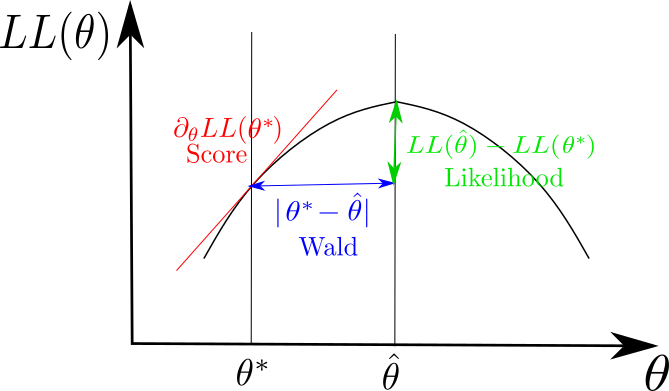
\includegraphics[width=3.2in]{conventions/classic-trio.png}
\caption{For $n=1$ and $\theta\in\RR$,
this figure shows the geometrical significance of
certain
quantities that
characterize the
3 classic test statistics
(Likelihood, Score, Wald)
for hypothesis testing.}
\label{fig-classic-trio}
\end{figure}

Henceforth in this section,
we will
occasionally  use the
Einstein summation
convention; i.e., implicit sum over
repeated indices.

Three classic test statistics
are (See Fig.\ref{fig-classic-trio}):

\begin{enumerate}

\item
{\bf Likelihood Ratio test statistic}
(Ref.\cite{wiki-Li-test}.)

\beq
\lam_{Li}=
2\ln\left[
\frac{L(\HAT{\theta})}
{L(\theta^*)}
\right]=
2[LL(\HAT{\theta})-LL(\theta^*)]
\eeq

\item
{\bf Score (a.k.a.
Lagrange multiplier) test statistic}
(Ref.\cite{wiki-Sc-test}.)

\beqa
\lam_{Sc}&=&
\partial_{\theta_i} LL(\theta^*)
\left[
FI(\theta^*)^{-1}\right]_{i,j}
\partial_{\theta_j} LL(\theta^*)
\\
&=&
\frac{[\partial_\theta LL(\theta^*)]^2}
{FI(\theta^*)}\quad \text{if $n=1$}
\eeqa
Doesn't depend on $\HAT{\theta}$.

\item
{\bf Wald test statistic}
(Ref.\cite{wiki-Wa-test}.)


\beqa
\lam_{Wa}&=&
(\HAT{\theta}-\theta^*)_i
\left[
\av{\HAT{\rvtheta},\HAT{\rvtheta}^T}^{-1}
\right]_{i,j}
(\HAT{\theta}-\theta^*)_j
\label{eq-wald-stat}
\\
&=&
\frac{(\theta^*-\HAT{\theta})^2}
{\av{\HAT{\theta},\HAT{\theta}}}
\quad\text{if $n=1$}
\eeqa

More generally,
one can replace $\theta^*\rarrow R\theta^*$
and  $\HAT{\theta}\rarrow R\HAT{\theta}$
in Eq.(\ref{eq-wald-stat}),
where $\theta^*$ and
$\HAT{\theta}$ are $n$ dimensional
column vectors, and
$R\in\RR^{\nu\times n}$.
The null and alternative hypotheses become:
$H_0: R\theta=R\theta^*$
and $H_1: R\theta\neq R\theta^*$.
Note that
$\nu$
is the number of
constraints imposed by the
null hypothesis. $R$ is called a
reparametrization of $\theta$.
The Wald test is not
reparametrization
invariant (i.e., $R$
invariant), but the Likelihood Ratio test is.

\end{enumerate}

Note that
if $LL(\theta)$
is given by Eq.(\ref{eq-normal-ll}),
then
$\av{\HAT{\rvtheta},\HAT{\rvtheta}}
=
\s^2=\frac{1}{FI(\theta)}
$. Hence,

\beq
\lam_{Li}=\lam_{Sc}=\lam_{Wa}=
\frac{(\HAT{\theta}-\theta^*)^2}{\s^2}
\eeq

Many
other commonly used test statistics
(or their squares)
are special cases of one
of the 3 classic test statistics.
For example, the z-statistic
used with normal
distributions,
the t-statistic
used with the
Student t-distribution,
the F-statistic used in linear regression,
the chi-squared statistic used
to do Pearson's chi-squared test.

{\bf Asymptotic Behavior}

If the data
$\vec{x}$ is i.i.d.,

\beq
P(\vec{x}|\theta)=
\prod_{\s=0}^{nsam-1} P(x^\s|\theta)
\;
\eeq
Hence, as $nsam\rarrow \infty$,

\beqa
LL(\theta)
&=&
\ln P(\vec{x}|\theta)
\\
&=&\sum_\s \ln
P(x^\s|\theta)
\\
&\rarrow&
nsam \sum_x P(x|\theta)\ln  P(x|\theta)
\\
&=&
-nsam \; H(\rvx|\theta)
\eeqa
Thus, {\it maximizing} the log likehood
$LL(\theta)$
and {\it minimizing} the entropy
$H(\rvx|\theta)$
give the same estimate $\HAT{\theta}$.

When the
data is i.i.d. and
$nsam\rarrow \infty$,
it is also possible to
prove that
the 3 test statistics
defined above all tend to
the same
probability  distribution, namely
$\calx^2(\theta^*; \nu)$,
the chi-square distribution
with $\nu$ degrees of freedom,
where $\theta\in \RR^n$, $R\in \RR^
{\nu\times n}$, and $\nu=n$ if $R=1$.

\section{Error Bars}
Never report measurements without error bars!!

Assume a distribution
with mean $\mu$ and
standard deviation $\s$
for a subpopulation with $n$
samples.

$SE=\frac{\s}{\sqrt{n}}$
is called the {\bf standard error}.


Some popular types of error bars:


\begin{itemize}
\item{\bf Box and Whiskers plot (a.k.a. Boxplot)}

See Fig.\ref{fig-boxplot}.
$IQR$ stands for {\bf
Intermediate Quantile Range}.
Sometimes, the endpoints of the
error bars are taken to be the minimum and maximum samples
instead of $Q_1- 1.5 *IQR$ and $Q_3+ 1.5 *IQR$.
The points that fall
in the intervals $[\min,Q_1- 1.5* IQR]$
and $[Q_3+ 1.5 *IQR, \max]$
are
called {\bf outliers}.
\begin{figure}[h!]
\centering
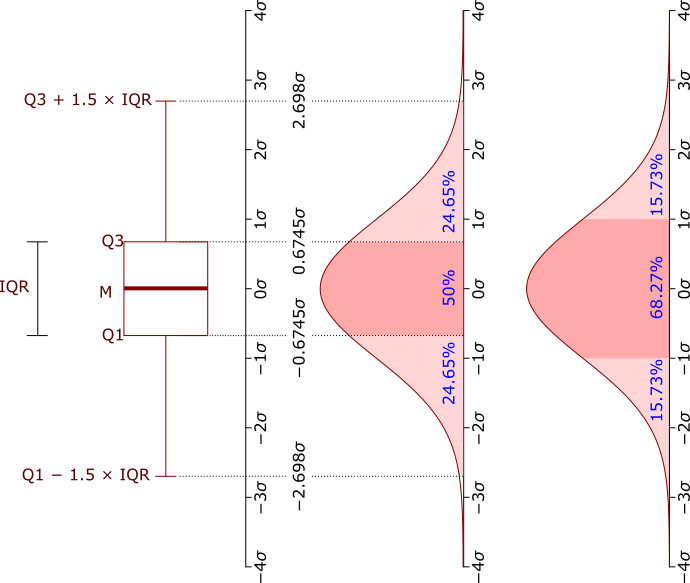
\includegraphics[width=3.3in]
{conventions/Boxplot.png}
\caption{Boxplot plot for Normal
distribution $\caln(\mu=0,\s)$.
$Q_1$ and $Q_3$ are the first and third
quantiles, and $M$ is the median (i.e., half-way point).
For a non-normal skewed
distribution, $Q_1$ and $Q_3$
are not equidistant from the median, and the
median is not exactly equal to the mean. }
 \label{fig-boxplot}
\end{figure}



\item{\bf Standard Deviation}

Error bar endpoints are located one standard deviation
away from the mean.
\beq
\mu-\s< \mu < \mu+\s
\eeq

\item{\bf Confidence Interval}

\beq
\mu-|z^*|SE <\mu < \mu+|z^*|SE
\label{eq-conf-int}
\eeq

$|z^*|=1.96$ for a confidence level of $95\%$.

The origin of Eq.(\ref{eq-conf-int})
is explained in the next section entitled ``Confidence Intervals".
Confidence intervals are
derived from the Gaussian in Fig.\ref{fig-conf-int},
which should not be confused with the
Gaussian of Fig.\ref{fig-boxplot}.
They are different!

\end{itemize}
\section{Confidence Interval}

Normal distribution
with mean $\mu$
and standard deviation $\sigma$:

\beq
\caln(x;\mu, \s^2)=
\frac{1}{\s\sqrt{2\pi}}
e^{-\;\frac{(x-\mu)^2}{2\sigma^2}}
\;.
\eeq

Standard Normal Distribution (SND):
\beq
P(z)=\caln(z;0,1)
\eeq
Cumulative distribution for $P(z)$:

\beq
\Phi(z)=\int_{-\infty}^z dz'\;P(z')
\;.
\eeq

\begin{figure}[h!]
\centering
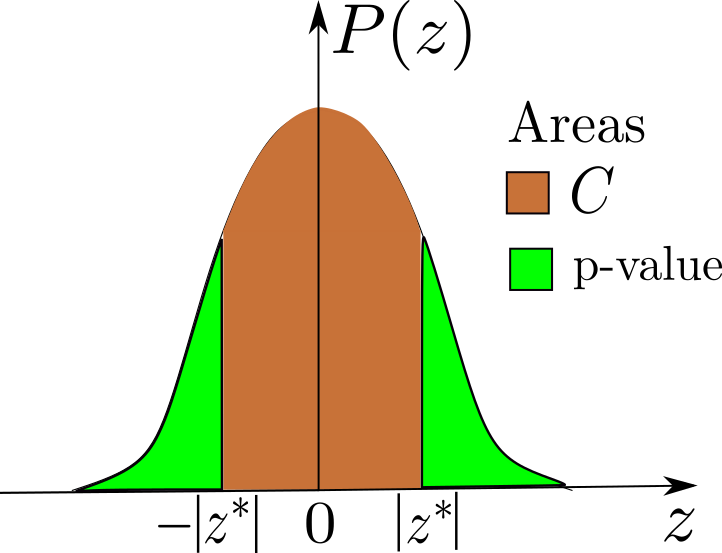
\includegraphics[width=2in]
{conventions/conf-int.png}
\caption{
Interpretation
of confidence level $C$
and p-value as areas under curve of the
Standard Normal Distribution (SND).}
\label{fig-conf-int}
\end{figure}

{\bf Confidence Level} $C$
and corresponding {\bf $|z^*|$ value}
(see Fig.\ref{fig-conf-int}):

\beq
C=\int_{-|z^*|}^{|z^*|} dz\;P(z) =
\Phi(|z^*|)-\Phi(-|z^*|)
=
2\left(\Phi(|z^*|)-\;\frac{1}{2}\right)
\label{eq-conf-level1}
\eeq
Equivalent definition:

\beq
C=P\left(
\underbrace{
\frac{|\rvx-\mu|}{\frac{\sigma}{\sqrt{n}}}
}_{|\rvz|}
<|z^*|\right)
\label{eq-conf-level2}
\eeq
For $C=95\%$,
$|z^*|=1.960\approx 2$.
For $C=99\%$, $|z^*|=2.576$.

Area of each tail
in Fig.\ref{fig-conf-int} is
usually called $\alpha$,
and the area of both tails is called
the {\bf p-value}:
\beq
C+\underbrace{2\alpha}_{p-value}=1
\;.
\eeq

Estimators\footnote{Don't
confuse the sample index $\s$
with the standard deviation $\s$.} of
mean $\mu$  and
standard deviation $\sigma$
from measurements $x^\s$
of a sub-population $\Sigma_1$ of
size $n=|\Sigma_1|$:
\beq
\HAT{\mu}=\ol{x}=\frac{1}{n}\sum_{\s \in\Sigma_1} x^\s
\eeq

\beq
\HAT{\s}^2=
\frac{1}{n-1}
\sum_{\s\in \Sigma_1} (x^\s-\ol{x})^2
\eeq


We get
from Eq.(\ref{eq-conf-level2}),
the {\bf Error bars (a.k.a. confidence intervals)}
and
{\bf Error $E$ (a.k.a. margin of error)}:



\beq
\text{ estimate of $x$
with error bars} =
\ol{x} \pm
\underbrace{
|z^*| \frac{\HAT{\s}}{\sqrt{n}}}_{E}
\label{eq-err-bars}
\eeq

\beq
n= \left(
\frac{|z^*|\HAT{\s}}{E}
\right)^2
\eeq

So far, we have assumed
that the sub-population (a.k.a. sample
population)
is normally distributed.
This might be false
for several reasons.
Some red flags: (1)
$n$ is too small (according to
a rule of thumb derived from
Central Limit Theorem, $n$
should be larger than 30
to insure a Normal Distribution).
(2) Sub-population not truly random
(i.i.d.)
because was taken
without replacement.
In many cases,
especially
when $n<30$,
the Student's t-distribution
models the sub-population statistics
much
better than the Normal distribution.


The {\rm Student's t-distribution } ${\rm Stud}(t;
\nu=n-1)$,
depends
on a parameter $\nu$
called the
number of
degrees of freedom.
In the case being considered here,
$\nu$ equals the
sub-population size $n$
minus one.
When fitting
the data with
Stud(), variable
$t$ replaces
variable $z$,
and ${\rm Stud}(t; \nu=n-1)$
replaces the Standard Normal distribution (SND)
$\caln(z; \mu=0, \sigma=1)$.
Stud() is symmetric about
the origin like SND,
but its tails
are fatter.
When fitting the data with Stud(),
the $|z^*|$
value is replaced
by a $|t^*|$ value.
Eq.(\ref{eq-conf-level1})
is replaced by


\beq
C=\int_{-|t^*|}^{|t^*|} dt\;{\rm Stud}(t) =
\Phi_S(|t^*|)-\Phi_S(-|t^*|)
=
2\left(\Phi_S(|t^*|)-\;\frac{1}{2}\right)
\label{eq-conf-level1-stu}
\;,
\eeq
where $\Phi_S()$
is the cumulative
distribution for  Stud().
Also, Eq.(\ref{eq-err-bars})
is replaced  by

\beq
\text{estimate of $x$
with error bars} =
\ol{x} \pm
\underbrace{
|t^*| \frac{\HAT{\s}}{\sqrt{n}}}_{E}
\;.
\eeq
Tables of $|t^*|(C,\nu=n-1)$
are available. Note
that $|t^*|$
depends on both $C$ and $\nu$,
whereas $|z^*|(C)$
depends only on $C$.

\section{p-value}


Given a parameter $\theta$, call
$\theta=\theta_0$ (or  $\theta<\theta_0$ or $\theta>\theta_0$) the
{\bf null hypothesis} $h_0$,
and call the negation of $h_0$ (i.e., 
$\theta\neq\theta_0$ (or  $\theta\geq\theta_0$ or $\theta\leq \theta_0$))
the {\bf alternative hypothesis} $h_1$.
Assume we
are given data $\vec{x}=\{x^\s|\s\in \Sigma\}$. Assume
also that we are given
distributions $P(\rvx=x|h)$ for $h\in \{h_0, h_1\}$,
and $P(\rvx=x)$. Now let

\beq
P(\vec{x}|h)=\prod_\s P(\rvx=x^\s|h)
\eeq


\beq
P(\vec{x})=\prod_\s P(\rvx=x^\s)
\eeq
(so the $x^\s$ are i.i.d.).

A Bayesian would assume that there
is a prior $P(h)$, and use it to
calculate
$P(h|\vec{x})=\frac{P(\vec{x}|h) P(h)}{P(\vec{x})}$.
$P(\rvh= h_0|\vec{x})$
is the probability that the null hypothesis is true.
A p-value is a monotonically increasing function of
$P(\rvh= h_0|\vec{x})$,
so Bayesians have no trouble saying
that  {\color{red} a p-value is
a measure of
$P(\rvh= h_0|\vec{x})$, i.e.,
a measure of the probability that
the null-hypothesis is true}.

Frequentists, on the other hand,
believe that $h$
is a ``parameter", not a random variable,
so  $P(\rvh= h_0|\vec{x})$
is undefined.
Next, we explain the correct
way of thinking about p-values, according to
Frequentists.
p-values were invented by Frequentists,
so it's worth hearing what they have to say
about them.
The Frequentist definition is not against Bayesianism,
and Bayesians, unlike Frequentists,
 don't accuse Frequentists of
having a sinfully incorrect
 definition of p-values. A Bayesian would just say:
our definition of p-values (shown
in red above) is not incorrect,
but the Frequentist definition is more precise than ours,
and doesn't assume a particular form for a prior.
We welcome it.

Call
the random variable
$\rvt$ the {\bf test statistic} and let 
$t^*$ be a user defined
parameter.
$\rvt$ and $t^*$
are defined so that
when $\rvt=t^*$,
the $h_0$ hypothesis is
on the threshold between 
being and not being satisfied.
Frequentists define the {\bf p-value} $p$ as

\beq
p=
\left\{
\begin{array}{ll}
P(\rvt \geq t^*|h_0)&\text{right-sided-tail,
if $h_0$ is $\theta<\theta_0$}
 \\
 P(\rvt\leq t^*|h_0)&\text{left-sided-tail,
 if $h_0$ is $\theta>\theta_0$}
 \\
 P(|\rvt| > |t^*|\;|h_0)&\text{double-sided-tail,
 if $h_0$ is $\theta=\theta_0$}
\end{array}
\right.
\eeq
Thus, for a Frequentist,
{\color{red} a p-value is a probabilistic
weight of the region
where the $h_0$ hypothesis is
defined (by the user) to be violated}.
If that weight is large,
then the region where
the $h_0$ hypothesis is
defined to be satisfied is small,
which means the $h_0$
hypothesis
is expected to be close to the truth.
The larger the p-value,
the closer $h_0$
is expected to be near the truth,
just like the Bayesian definition
says.
Note that the p-value
is a probability so it ranges in
value from 0 to 1.

Suppose we are given a subpopulation with $n$ samples,
 mean $\ol{x}$ and variance $\HAT{\s}$.
 Let $\theta_0=\mu_0$.
Define

\beq
\rvt=\rvz=
\frac{\rvx-\mu_0}{\frac{\HAT{\s}}{\sqrt{n}}}
\;. 
\eeq
For $n>30$, 

\begin{subequations}
\beqa
P(\rvz\geq z^*|h_0)
=1-\Phi(z^*)=\Phi(-z^*)
&\quad&\text{if $h_0$ is $\mu<\mu_0$}
\\
P(\rvz\leq z^*|h_0)=\Phi(z^*)
&\quad&\text{if $h_0$ is $\mu>\mu_0$}
\\
P(|\rvz|\geq |z^*|\;|h_0)=2\Phi(-|z^*|)
&\quad&\text{if $h_0$ is $\mu=\mu_0$}
\label{eq-double-tail}
\eeqa
\end{subequations}
where $\Phi(x)$ is the cumulative distribution
for the Standard Normal Distribution
$\caln(x;\mu=0, \s=0)$.
For $n<30$, $\Phi()$ is replaced
by $\Phi_S()$, where  $\Phi_S()$ is
the cumulative distribution
for the Student t-distribution ${\rm Stud}(x; \nu=n-1)$.
Note that Eq.(\ref{eq-double-tail})
agrees with
Eq.(\ref{eq-conf-level2}).

The quantity
\beq
z_{score}=
\frac{\ol{x}-\mu_0}{\frac{\HAT{\s}}{\sqrt{n}}}
\eeq
is called the {\bf z score}.
If $|z_{score}| > |z^*|$,
then the $h_0$ hypothesis
is defined to be violated
(for the double sided case).

\section{Short Summary of
Boolean Algebra}
See Ref.\cite{wiki-bool} for more info
about this topic.

Suppose $x, y, z\in \bool$. Define

\beq
x\text{ or }y=x\V y= x+y-xy
\;,
\eeq

\beq
x \text{ and }y=x\A y= xy
\;,
\eeq
and

\beq
\text{not }x=\ol{x}=1-x
\;,
\eeq
where we are using
normal addition and multiplication
on the right hand sides.\footnote{Note the
difference between $\V$ and modulus
2 addition $\oplus$.
For $\oplus$ (a.k.a. XOR): $x\oplus y=x+y-2xy$.}



\begin{table}[h!]
\centering
\begin{tabular}{|
>{\columncolor[HTML]{ECF4FF}}l |l|}
\hline
Associativity & \begin{tabular}[c]{@{}l@{}}$x \V (y \V z)=(x \V y) \V z$\\ $x \A (y \A z)=(x \A y) \A z$\end{tabular} \\ \hline
Commutativity & \begin{tabular}[c]{@{}l@{}}$x \V y=y \V x$\\ $x \A y=y \A x$\end{tabular} \\ \hline
Distributivity & \begin{tabular}[c]{@{}l@{}}$x \A (y \V z)=(x \A y) \V (x \A z)$\\ $x \V (y \A z)=(x \V y) \A (x \V z)$\end{tabular} \\ \hline
Identity & \begin{tabular}[c]{@{}l@{}}$x \V 0=x$\\ $x \A 1=x$\end{tabular} \\ \hline
Annihilator & \begin{tabular}[c]{@{}l@{}}$x \A 0=0$\\ $x \V 1= 1$\end{tabular} \\ \hline
Idempotence & \begin{tabular}[c]{@{}l@{}}$x \V x= x$\\ $x \A x= x$\end{tabular} \\ \hline
Absorption & \begin{tabular}[c]{@{}l@{}}$x \A (x \V y)= x$\\ $x \V (x \A y)= x$\end{tabular} \\ \hline
Complementation & \begin{tabular}[c]{@{}l@{}}$x \A \ol{x} = 0$\\ $x \V \ol{x}   = 1$\end{tabular} \\ \hline
Double negation & $\ol{(\ol{x})} = x$ \\ \hline
De Morgan Laws & \begin{tabular}[c]{@{}l@{}}$\ol{x} \A \ol{y} =\ol{(x \V y)}$\\ $\ol{x} \V \ol{y} = \ol{(x \A y)}$\end{tabular} \\ \hline
\end{tabular}
\caption{Boolean Algebra Identities}
\label{tab-bool-alg}
\end{table}

Actually, since
$x\A y=xy$, we can omit writing
the symbol $\A$. The symbol
$\A$ is useful to
exhibit the symmetry
of the identities, and
to remark
about
the analogous identities
for sets, where
$\A$ becomes intersection $\cap$
and $\V$ becomes union $\cup$. However,
for practical calculations,
$\A$ is an unnecessary nuisance.

Since $x\in \bool$,
\beq
P(\ol{x})=1-P(x)
\;.
\eeq

Clearly, from analyzing
the simple event space $(x,y)\in \bool^2$,
\beq
P(x\V y)= P(x) + P(y) - P(x\A y)
\;.
\eeq

\section{Definition of a Bayesian Network}
\label{ch-bnet-def}

A {\bf directed graph} $G=(V,E)$
consists of two sets, $V$
and $E$. $V$ contains
the {\bf vertices (nodes)}
and $E$ contains the {\bf edges (arrows)}.
An arrow $a\rarrow b$ is an
ordered pair 
$(a,b)$ where $a, b\in V$.
The {\bf parents} 
of a node $x$ are 
those nodes $a$
such that there are arrows 
$a\rarrow x$.
The {\bf children} of a node
$x$
are those nodes $b$
such that there are arrows $x\rarrow b$.
The {\bf neighbors}
of a node $x$
is the set of parents and 
children of $x$.
A {\bf path} is a 
set of nodes that 
are connected 
by arrows, so 
that all nodes
have 1 or 2 neighbors,
but only two nodes ({\bf open path})
or zero nodes ({\bf closed path})
have only one neighbor.
A {\bf directed path}
is a path in
which all the arrows point
in the same direction.
A {\bf loop}
is a closed path;i.e.,
a path in which all
nodes have exactly 2 neighbors.
A {\bf cycle} is a directed loop.
A {\bf Directed Acyclic Graph (DAG)}
is a directed graph that has no
cycles. 


A {\bf fully connected directed graph}
is 
a directed graph
in which 
every node has all other 
nodes as neighbors.
Figs.\ref{fig-full-conn-4-line}
and
\ref{fig-full-conn-4-square}
show 2 different
ways of drawing
the same directed graph,
a fully connected graph with 4 nodes.
Note that a convenient
way
to label
the nodes of a fully
connected directed
graph
with $N$ nodes
is to point
arrows
from 
$\rvx_k$ to $\rvx_j$
where $j=0, 1, 2,\ldots, N-1$
and 
$k=j-1, j-2, \ldots, 0$.


\begin{figure}[h!]
$$
\xymatrix{
\rvx_3
&\rvx_2\ar[l]
&\rvx_1\ar[l]\ar@/_1pc/[ll]
&\rvx_0\ar[l]\ar@/_2pc/[ll]\ar@/_2pc/[lll]
}
$$
\caption{Fully 
connected directed  graph with 4 nodes,
drawn as a line.}
\label{fig-full-conn-4-line}
\end{figure}

\begin{figure}[h!]
$$
\xymatrix{
\rvx_0\ar[r]\ar[d]\ar[rd]&\rvx_1\ar[d]\ar[ld]
\\
\rvx_2\ar[r]&\rvx_3
}
$$
\caption{Fully 
connected directed  graph with 4 nodes,
drawn as a square.}
\label{fig-full-conn-4-square}
\end{figure}

\hrule

A {\bf Bayesian network (bnet)}
consists of a DAG 
and a 
{\bf Transition 
Probability Matrix (TPM)}
associated 
with each node
of the graph.
A TPM is often 
called a {\bf Conditional Probability
Table 
(CPT)}.
The {\bf structure} of a bnet
is its DAG alone, sans the TPMs.


In 
this book,
random  variables are
 indicated by 
underlined letters and their values 
by non-underlined letters.
 Each node of a bnet is
 labelled by a random variable.
 Thus, $\rvx=x$ means that node 
$\rvx$ is in state $x$.


\hrule\noindent
{\bf Some sets of nodes 
associated 
with each node $\rva$
of a bnet}
\begin{itemize}
\item
$ch(\rva)=$ children of $\rva$.
\item
$pa(\rva)=$ parents of $\rva$.
\item
$nb(\rva)=pa(\rva)\cup ch(\rva)=$ 
neighbors of $\rva$.
\item
$de(\rva)=\cup_{n=1}^{\infty}ch^n(\rva)=$
$ch(\rva)\cup ch\circ ch(\rva)\cup\ldots$, 
descendants of $\rva$. 
\item
$an(\rva)=\cup_{n=1}^{\infty}pa^n(\rva)=$
$pa(\rva)\cup pa\circ pa(\rva)\cup\ldots$, 
ancestors of $\rva$.
\end{itemize}
\hrule
In this book,
we will use 
$\rva.$
to indicate
a {\bf multi-node (node set,
node array)} $\rva.=
(\rva_j)_{j=0, 1, \ldots , na-1}$.
We will often
treat multinodes as if
they were sets, and
combine them with
the usual
set
operators.
For instance,
for two
multinodes $\rva.$
and $\rvb.$,
we define
$\rva.\cup\rvb.$,
$\rva.\cap\rvb.$,
$\rva.-\rvb.$
and
$\rva.\subset\rvb.$
in the obvious way.
We 
will indicate
a singleton set (single
node multi-node) $\rva.=\{\rva\}$
simply by $\rva.=\rva$.
For instance,
$\rva.-\rvb=\rva.-\{\rvb\}$.
\hrule

The TPM of a node
$\rvx$ of a bnet
is a matrix of
probabilities 
$P(\rvx=x|pa(\rvx)=a.)$.

A bnet
with nodes $\rvx.$
represents
a probability
distribution

\beq
P(x.)=
\prod_j
P(\rvx_j=x_j|
(\rvx_k=x_k)_{k: \rvx_k\in pa(\rvx_j)})
\;.
\label{eq-chain-rule-bnet}
\eeq

Note that
for a fully connected bnet
with $N$ nodes,
Eq.(\ref{eq-chain-rule-bnet})
becomes

\beq
P(x.)=
\prod_{j=0}^{N-1}
P(x_j| 
(x_k)_{k=j-1, j-2, \ldots, 0})
\;.
\label{eq-chain-rule-cond-probs}
\eeq
For example, if $N=4$,
Eq.(\ref{eq-chain-rule-cond-probs})
 becomes

\beq
P(x_0, x_1,x_2, x_3)=
P(x_3|x_2, x_1, x_0)
P(x_2|x_1, x_0)
P(x_1|x_0)
P(x_0)
\;.
\eeq
We see that 
Eq.(\ref{eq-chain-rule-cond-probs})
is just the chain rule for 
conditional probabilities.






\chapter{Bayesian Networks, Causality and the
Passage of Time}
%\addcontentsline{toc}{chapter}{Bayesian Networks, Causality and the Passage of Time}

\label{ch-bnets-time}

This chapter is based
on a blog post (see Ref.\cite{bnets-passage-time})
from my blog ``Quantum Bayesian Networks".

\section{Unifying Principle of this book}
The unifying principle of this
book is Bayesian Networks (bnets).
The main goal of this book
is to explain
as much of Artificial Intelligence (AI)
and Machine Learning (ML)
as possible
using bnets.

Bayesian Networks are a graphical representation of the chain rule for
conditional probabilities.
 They are not a ``heuristic algorithm” like XGBoost or Neural Nets.
They are a very simple, intuitive, basic and general definition. I would say
that the definition of a Bayesian Network is as important to Probability
Theory as the definition of a Group is to Abstract Algebra. Algebraic groups
are never going to go out of fashion and neither are B nets.

An Artificial Neural Net can be defined as a Bayesian Network with a layered
structure, and such that all its nodes are deterministic\footnote{Neural Nets (NNs)
are DAGs, but they contain a lot of 
spurious arrows whose direction
or very existence has no causal motivation,
and they could be missing
other arrows which 
would have a causal motivation.
 So I like to
say that NNs are acausal DAGs.}. A decision tree
is not exactly a Bayesian Network, but it can be trivially replaced by an
equivalent B net that has the same tree structure (for more details about
this equivalence, see the Chapter \ref{ch-dtree} on decision trees).
The SCM diagrams favored by Pearl are just bnets
whose internal nodes are deterministic and external ones
are probabilistic.
In fact, as I show in this book, most methods in AI can be
understood in terms of B nets---just
like many theorems in Abstract Algebra
can be understood in terms of groups.



\section{You say tomato, I say tomato}
In this chapter, I will use the terms Bayesian Network
(bnet), causal model and DAG as if they were synonymous.
My justification for doing this is as follows.


 A Bayesian Network is a DAG + probability tables. One can easily compute the
 probability tables from DAG + Dataset. Therefore,

You say DAG+Dataset, I say Bayesian Network.

The use of the terms ``causal model” and ``DAG”, as an alternative to the term
``Bayesian Network”, has become popular in the last decade
among economists, epidemiologists,
AI researchers and even Judea Pearl himself. It seems some
people think ``causal models” and ``DAGs” are revolutionary, whereas Bayesian
Networks are a concept that was tried 25 years ago, and has been replaced
since then by stuff that works better. But any time you have a Dataset, which
is almost always true in practice in Economics,
Epidemiology  and AI, a DAG implies a
Bayesian Network and vice versa.



\section{A dataset is causal model free}
Time and time again, Judea Pearl makes the point on Twitter to neural net
advocates that they are trying to do a provably impossible task,
 to derive a
causal model from data. I could be wrong, but this is what I think he means.

When Pearl says ``data”, he is referring to what is commonly called a dataset.
A {\bf dataset} is a table of data, where all the entries of each column have
the
same units, and measure a single feature, and each row refers to one
particular sample or individual. Datasets are particularly useful for
estimating probability distributions and for training neural nets. When Pearl
says a ``causal model", he is referring to a DAG (directed acyclic graph) or a
bnet
(Bayesian Network= DAG + probability table for each node of DAG).

Sure, you can try to derive a causal model from a dataset,
 but you’ll soon find
 out
that you can only go so far.

The process of finding a partial causal model from a dataset is called
structure
learning (SL).  SL can be done quite nicely with Marco Scutari’s open source
program bnlearn. There are 2 main types of SL algorithms: score-based and
constraint based. The first and still very competitive constraint-based SL
algorithm was the Inductive Causation (IC) algorithm proposed by Pearl and
Verma in 1991. So Pearl is quite aware of SL. The problem is that SL often
cannot narrow down the causal model to a single one.
It finds an undirected
graph
(UG), and it can determine the direction of some of the arrows in the UG, but
it is often incapable, for well understood fundamental
---not just technical---
reasons, of finding the direction of ALL the arrows of the UG. So it often
fails to fully specify a DAG model.

Let’s call the ordered pair
(dataset, causal model) a
dataset++ . Then what I
believe Pearl is saying is that a
dataset is causal model-free or causal model-less
(although sometimes one can find a partial
causal model hidden in there). A dataset
is not a dataset++.

{\bf Caveat to this section:} Define a {\bf time-series table (TST)} to be
a table of data, where all the entries of each column have
the
same units, and measure a single feature at different times with time increasing down the table.
Hence, the rows of a TST are chronologically ordered (they 
specify a time series)
whereas those of a dataset aren't. Whereas it is not possible to
fully specify a DAG from a dataset alone, it is possible
to do so from a TST. See the python app CausalFit (Ref.\cite{CausalFitbit}) for a possible
way extracting a causal DAG from a Fitbit TST.

\section{What is causality?}
What is Causality, really, and how do Bayesian Networks
(a.k.a. Causal Models,
DAGs) encode it?
For me, Causality is a time-induced ordering between two events, the
transmission of information (and its accompanying
energy) from the earlier of the two events to the later
one, and the physical response of the later event to the reception of that
information. 

Note that this definition
of causality does not mention
correlation.
It is often assumed that even though
correlation does not imply causation,
causation implies correlation.
But the latter statement is false; there
are scenarios, albeit  unusual,
``fine tuned" ones,
in which there is causation
without correlation.
For example, 
consider a bnet 
with arrows $\rvx\rarrow \rvy$
and $\rvx\rarrow \rvc \rarrow \rvy$.
When we amputate 
the arrows entering $\rvx$,
a dependence
between $\rvx$ and $\rvy$ persists,
so we say $\rvx$ causes $\rvy$.
Even
though $\rvx$ causes $\rvy$,
it's possible to tune the 
probabilities
of the bnet so that
the effect of the path $\rvx-\rvc-\rvy$
and the effect of the direct path $\rvx-\rvy$
cancel 
each other out and
produce zero 
correlation between $\rvx$ and $\rvy$.
As a trivial example, suppose
$\rvc=2\rvx$, $\rvy=\rvc-2\rvx=0$.
Since $\rvy=0$, it's uncorrelated with $\rvx$.

The nodes of a bnet represent random variables. Some of those
random variables are clearly events (i.e., they occur at a definite time).
For example, let D=0 if a patient is not given a drug, D=1 if he/she is given
it. D occurs at a definite time. But other random variables represent
qualities which do not occur at a definite time. For example,
G=gender=male, female. G does not occur at a definite time.  But even in the
case of a quality like G, its value is first decided at birth, so one can
ascribe to G a particular, albeit fuzzy time interval during which it is
decided. If M=0(single), 1(married), then we can assign to M the day of the
marriage. Both the time interval assigned to G and to  M are somewhat
ambiguous, but still, most people would say that G occurs before M (if a
marriage occurs at all). Saying the opposite, that M occurs before G, seems
pretty hard to understand. If two nodes A and B of a bnet have time intervals
ascribed to them such that the time interval of A does not clearly occur
before or after the time interval of B, and if also there is a large causal
correlation between A and B, then it probably does not matter
much whether one draws an arrow from A to B, or the opposite.

Now that we understand that the arrows in a bnet really do encode the
direction of time, it becomes clear why a dataset does not fully specify a
bnet. By a dataset (think of a dataframe in Pandas or R), I mean an array of
numbers where the columns refer to features and the rows refer to individuals
in a population. The column labels of the dataset become the node names of
the bnet. Nowhere in a dataset is there any indication of the time ordering
of the features. Hence, it’s impossible to create, from a dataset alone, a
bnet, because bnets do carry such time-ordering information.

Chapter \ref{ch-granger-c} discusses
 Granger Causality
(GC). The critics of GC point out that it assumes, somewhat erroneously,
that if event A precedes B and the two events are correlated, A must
cause B. I agree. Most roosters crow in response to the stimulus of the
sunrise light.  A rooster could crow before sunrise if,  for example,  he
had an alarm clock that woke him up 30 minutes before sunrise, but such cases
are uncommon, and seem to involve other intermediate events.  The moral is
that time ordering and correlation are not sufficient
conditions for causality. To establish causality with more certainty, one
also needs a pinch of prior expert knowledge, or one must gain that expert
knowledge through ``do” operator experimentation.



\section{Bayesian Networks and the passage of time}

Now that we understand that a bnet’s arrows are encoding roughly the passage
of time, it becomes possible to glean from this insight a simple method,
which, although not very rigorous, is really helpful to me. I will illustrate
said method with the famous ``Asia” bnet in Fig.\ref{fig-asia}.
 In this bnet, all nodes
have two  possible values, 0 and 1.

\begin{figure}[h!]
\centering
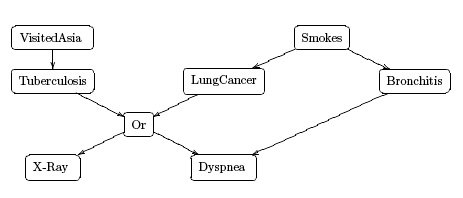
\includegraphics[width=5in]
{bnets-time/asia.jpg}
\caption{Asia bnet. Dyspnea=trouble breathing}
\label{fig-asia}
\end{figure}


Given a dataset for this bnet, one can calculate the correlation between
every 2 features of the dataset. The feature names become the node names, and
links are drawn between any 2 nodes whose correlation is 
causal and greater in absolute
value to some threshold value.
This gives an undirected graph that can be
obtained from bnet Fig.\ref{fig-asia}
 by erasing the directions of the arrows. So how
can we guess the directions of the arrows? Well, one uses a little bit of
``expert knowledge” to conclude that

time(Visited Asia) $<$ time(Tuberculosis) $<$ time(Or) $<$ time(X-Ray,
Dyspnea)

Also

time(smokes) $<$ time(LungCancer, Bronchitis) $<$ time(Or) $<$ time(Dyspnea)

If time(A) $<$ time(B), then A $\rarrow$ B. Like I
said before, the times we ascribe to
these events are somewhat fuzzy and open to debate, so this algorithm is far
from being rigorous. But often, saying that  time(A)$<$time(B) makes much more
sense than saying that time(B)$<$time(A). When in doubt about the best
direction to give to an arrow of an undirected graph, I recommend calculating
a Goodness of Causal Fit metric (see Chapter
\ref{ch-good-causal-fit}) which makes use of ``do” operator
experimentation.


A dataset cannot fully specify a
bnet because it lacks time ordering info. A dataset also cannot do the harder
task of specifying a bnet that is a good causal fit to the problem, because
it lacks time ordering info AND prior expert knowledge AND expert knowledge
gained from posterior ``do” operator experimentation.

\section{Advice for the DAG-phobic}
\label{sec-advice-dagophobic}

DAGs are your friends. DAGs should be easy and fun to dream up. After all, I
am convinced that DAGs are an integral part of how humans think, so they
should come naturally to us.  Nevertheless, many people are scared of, or
detest, DAGs. I think it’s because they fail to grasp the following 3 things:

1. DAGs are not unique. Stop thinking that you have to find the unique DAG
for the situation being considered. You just have to find a DAG that is a
good causal fit for the situation. If a DAG is too complicated, you can
always simplify it by merging several nodes into a single more abstract one,
or by summing over unwanted nodes.

2. The nodes of a DAG are roughly ordered from past to present. The arrows of a DAG roughly
reflect the passage of time.

3. DAGs represent scientific hypotheses that can and should be tested with
do experiments. Causal Inference is an
application of the scientific method, which consists
of the following steps:
formulate hypothesis (DAG), devise experiment
to test it, test it.

\chapter{AdaBoost}
\label{ch-adaboost}

This chapter
is based on Ref.\cite{wiki-adaboost}.


Adaptive Boosting (AdaBoost) is 
a method of constructing
a strong
classifier function
as a linear 
combination
of an ensemble
of weak classifier
functions.

Below,
we will abbreviate
``ensemble classifiers" by ``e-classifiers"
and ``weak classifiers' by ``w-classifiers".


Chapter \ref{ch-dtree}
defines decision trees (dtrees)
and explains how to construct them.
A
{\bf tree stump}
is a dtree  with only one
parent and 2 children nodes.
Usually the 
w-classifier functions
for AdaBoost
come from tree stumps
(because tree stumps
are w-classifiers
and simple to compute), but
the core
AdaBoost algorithm
is oblivious to 
where the w-classifier functions came from.


Chapter \ref{ch-rforest}
is on Bagging (Random Forest),
which is 
another method
besides AdaBoosting
of building a classifier function
from an ensemble 
of classifier functions.
These two methods are most commonly
applied to dtrees: AdaBoosting for an ensemble of
tree stumps, and Bagging for a random 
forest (which
is an ensemble
of dtrees that are usually much more
complicated than tree stumps). Both methods 
 are highly effective
in mitigating overfitting,
a common problem with simple
dtrees.


\section{AdaBoost for general ensemble
of w-classifiers}
In this 
section 
we discuss the core Adaboost
algorithm,
valid for a generic ensemble of w-classifiers.

Let $L=[0,1,2, \ldots, nsam-1]$ be a list of
individuals (samples) in a population.
In this chapter, we will use the notation 
$A^\s=A[\s]$ 
and $\vec{A}=[A^\s:\s\in L]$
for a  list (vector, 1-D  array) indexed by $L$.
We will refer to $DS=(\vec{x}, \vec{y})$ 
where $x^\s\in S_\rvx$, $y^\s\in S_\rvy$,
as a dataset. 
Let $T=\{0,1, \dots, nt-1\}$.
Let
$x^\s=(x^\s_0, x^\s_1, \ldots, x^\s_{nt-1})
\in S_{\rvx_0}\times S_{\rvx_1}
\times\ldots\times
 S_{\rvx_{nt-1}}=S_\rvx$.

AdaBoost assumes
that the classifier class set
$S_\rvy$  and
all the feature sets $S_{\rvx_t}$ 
are
binary:
$S_\rvy=S_{\rvx_t}=\{-1, 1\}$ for 
all $t\in T$.


Suppose that we are given an
ensemble of $nt$
{\bf w-classifiers}
$Y_t:S_\rvx\rarrow \{-1, 1\}$,
where $t\in T$.
Suppose we
 want to find  {\bf intermediate 
e-classifiers}
$\caly_t:S_\rvx\rarrow \RR$ 
given by 

\beq
\caly_t(x^\s)=
\sum_{t'=0}^t\alp_{t'}Y_{t'}(x^\s)
\in \RR
\eeq
for $t\in T$
and a {\bf final e-classifier}
given by 

\beq
\caly_{fin}(x^\s)=
sign\left(
\sum_{t=0}^{nt-1}\alp_t Y_t(x^\s)
\right)\in\{-1, 1\}
\;.
\eeq
The Adaboost algorithm 
yields a set of 
coefficients $\alp_t$
for which the final e-classifier
is much stronger (i.e., less error
prone) than any of the w-classifiers of the ensemble.

Note that
\beq
\caly_t(x^\s)=
\caly_{t-1}(x^\s)
+\alp_t Y_t(x^\s)
\eeq
for $t\in T$ if  we define
$\caly_{-1}=0$. Hence

\beq
\underbrace{e^{-y^\s \caly_t(x^\s)}}_
{Z_t w^\s_{t+1}}
=
\underbrace{e^{-y^\s \caly_{t-1}(x^\s)}}_
{Z_{t-1}w^\s_{t}}
e^{-\alp_t y^\s Y_t(x^\s)}
\eeq
where the {\bf weights}
$w_t^\s$ and 
and the {\bf
partition
function} $Z_t$ are defined by

\beq
w^\s_{t+1} = 
\left\{
\begin{array}{ll}
1/nsam&\text{for $t=-1$}
\\
\frac{\exp(-y^\s \caly_t(x^\s))}{Z_t}
&\text{for $t\geq 0$}
\end{array}
\right.
\eeq
and

\beq
Z_t =\sum_\s
e^{-y^\s \caly_t(x^\s)}
\;.
\eeq
Note that the probability
distribution 
$P(\s|t+1)=w^\s_{t+1}$
of weights 
at time $t+1$ emphasizes 
(i.e., gives higher probability to)
the errors (i.e., 
occurrences of $y^\s \caly_t(x^\s)=-1$
for some population
individual $\s$)
 of the previous (i.e., at time $t$)
intermediate 
e-classifier 
$\caly_t$.
In other words,
every new
intermediate 
e-classifier $\caly_{t+1}$
concentrates
on those individuals $\s$
on which the previous e-classifier $\caly_{t}$
performed poorly.

Note also that
the partition function $Z_t$ is
a good measure
of the {\bf classification error}
(i.e., 
occurrences of $y^\s \caly_t(x^\s)=-1$)
of $\caly_t$. We will
therefore use $Z_t$
for that purpose,
as an error measure.

For $t>1$, we have 
\beqa
Z_t
&=&
\sum_\s
e^{-y^\s \caly_t(x^\s)}
\\
&=&
\sum_\s 
\underbrace{e^{-y^\s \caly_{t-1}(x^\s)}}_
{Z_{t-1}w^\s_t}
e^{-\alp_t y^\s Y_t(x^\s)}
\\
&=&
Z_{t-1} E_\s[e^{-\alp_t y^\s Y_t(x^\s)}]
\eeqa
Define the {\bf success rate} by
\beqa
S_t&=&
\sum_\s w^\s_t\indi(y^\s Y_t(x^\s)=1)
\\
&=&
E_\s[\indi(\underbrace{y^\s Y_t(x^\s)=1}_
{\text{ iff }y^\s = Y_t(x^\s)}
)]
\eeqa
and the {\bf failure rate} by

\beqa
F_t&=&
\sum_\s w^\s_t\indi(y^\s Y_t(x^\s)=-1)
\\
&=& E_\s[\indi(
\underbrace{y^\s Y_t(x^\s)=-1}_
{\text{ iff }y^\s\neq Y_t(x^\s)}
)]
\;.
\eeqa
Note that 

\beq
S_t+F_t=1
\;,
\eeq
and

\beq
Z_t= Z_{t-1}(e^{-\alp_t}S_t
+
e^{+\alp_t}F_t)
\;.
\eeq

\begin{figure}[h!]
\centering
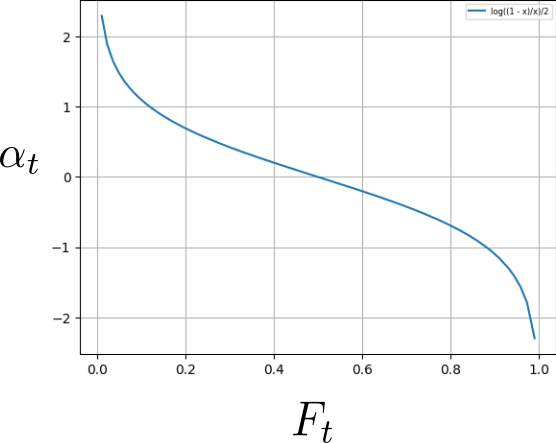
\includegraphics[width=3in]
{adaboost/adaboost-curve.png}
\caption{
Plot of function $\alp_t=
\frac{1}{2}\ln \frac{1-F_t}{F_t}$.
} 
\label{fig-adaboost-curve}
\end{figure}

We can find the $\alp_t$ values
that minimize the classification
error $Z_t$, and
then evaluate $Z_t$
at those optimum $\alp_t$ values:


\beq
\frac{d Z_t}{d\alp_t}
=Z_{t-1}(
-e^{-\alp_t}S_t
+
e^{\alp_t}F_t)
=0
\eeq

\beq
e^{2\alp_t}
=
\frac{S_t}{F_t}
\eeq

\beq
\alp_t=
\frac{1}{2}
\ln
\frac{S_t}{F_t}
=
\frac{1}{2}
\ln
\frac{1-F_t}{F_t}
\eeq

\beq
\frac{Z_t}{Z_{t-1}}=2\sqrt{S_tF_t}
=2\sqrt{(1-F_t)F_t}
\leq 1
\eeq
$f(x)=2\sqrt{(1-x)x}$
for $x\in[0,1]$
is dome shaped 
and its maximum 
is $1$,
which is
achieved iff $x=\frac{1}{2}$





\begin{figure}[h!]
$$
\xymatrix{
&
\rvY_0\ar[dr]\ar@/_1.5pc/[ddd]
&
\rvY_1\ar[dr]\ar@/_1.5pc/[ddd]
&
\rvY_2\ar[dr]\ar@/_1.5pc/[ddd]
&
\rvY_3\ar[dr]\ar@/_1.5pc/[ddd]
&
\rvY_4\ar@/_1pc/[ddd]
\\
(\vec{\rvx},\vec{\rvy})
\ar@/_1.5pc/[rr]
\ar@/_1.5pc/[rrr]
\ar@/_1.5pc/[rrrr]
\ar@/_1.5pc/[rrrrr]
&
\vec{\rvw}_0\ar[r]\ar[d]
&
\vec{\rvw}_1\ar[r]\ar[d]
&
\vec{\rvw}_2\ar[r]\ar[d]
&
\vec{\rvw}_3\ar[r]\ar[d]
&
\vec{\rvw}_4
\\
(\vec{\rvx},\vec{\rvy})
\ar@/_1.5pc/[r]
\ar@/_1.5pc/[rr]
\ar@/_1.5pc/[rrr]
\ar@/_1.5pc/[rrrr]
\ar@/_1.5pc/[rrrrr]
&
\ul{\alp}_0\ar[d]\ar[ru]
&
\ul{\alp}_1\ar[d]\ar[ru]
&
\ul{\alp}_2\ar[d]\ar[ru]
&
\ul{\alp}_3\ar[d]\ar[ru]
&
\ul{\alp}_4\ar[d]
\\
&
\ul{\caly}_0\ar[r]
&
\ul{\caly}_1\ar[r]
&
\ul{\caly}_2\ar[r]
&
\ul{\caly}_3\ar[r]
&
\ul{\caly}_4
}$$
\caption{Bnet for AdaBoost with
5 w-classifiers,
 $nt=5$.
All nodes labelled $(\vec{x},\vec{y})$
are the same node. 
}
\label{fig-aboost-bnet}
\end{figure}

The AdaBoost algo 
described
in this chapter is summarized
by
the bnet of Fig.\ref{fig-aboost-bnet}.
The TPMs, printed in blue, for the nodes of that
bnet, are as follows:

\beq\color{blue}
P(w^\s_0)=\frac{1}{nsam}
\;
\eeq
for all $\s$.

\beq\color{blue}
P(\vec{w}_{t+1}|\vec{w}_{t},
\alp_t, Y_t,    \vec{x}, \vec{y})=
\prod_\s
\indi(\;\;\; 
w^\s_{t+1} =\frac{ w^\s_t e^{-\alp_t y^\s Y_t(x^\s)}}
{\sum_\s numerator}
\;\;\;)
\eeq
for $t\geq 0$.


\beq\color{blue}
P(\alp_t|\vec{w}_t, \vec{x}, \vec{y})=
\indi(\;\;\; \alp_t=
\frac{1}{2}
\ln\frac{1-F_t}{F_t}
\text{ where }F_t=F_t(\vec{w}_t, \vec{x},\vec{y})\;\;\;) 
\eeq
for $t\in T$.

\beq\color{blue}
P(\caly_t| \caly_{t-1}, \alp_t, Y_t)
=
\indi(\;\;\;\caly_t= \caly_{t-1}+ \alp_t Y_t\;\;\;)
\eeq
for $t\in T$,
where $\caly_{-1}=0$.

\section{AdaBoost for ensemble of tree stumps}

Keep in mind that
AdaBoost assumes
$S_\rvy=S_{\rvx_t}=\{-1, 1\}$
for all $t\in T=\{0,1, \ldots, nt-1\}$.
In order to implement 
AdaBoost, we need to
specify 
$nt$
w-classifiers $Y_t:\{-1, 1\}^{nt}
\rarrow \{-1, 1\}$ for $t\in T$.
One can either
specify the $nt$ w-classifiers
a priori or build them
on-the-fly.

\begin{itemize}
\item {\bf
w-classifiers specified a priori}

Define a classifier 
for each feature $x_t$ 
where $t\in T$ by:

\beq
Y_t(x^\s)=x^\s_t\in \{-1, 1\}
\eeq
Hence, for this classifier,
$y^\s Y_t (x^\s)=y^\s x_t^\s$.

\item {\bf w-classifiers built
on-the-fly}

Recall
dataset
$(\vec{x},\vec{y})=
[(x^\s, y^\s):\s\in L]$
is indexed by the  list
 $L=[0, 1, \ldots, nsam-1]$.
If
$L_j$ is a list (possibly with 
duplicate items)
such that $set(L_j)\subset set(L)$,
 then
define
$DS_j=(\vec{x}, \vec{y})_{L_j}=
((x^\s)_{\s\in L_j}, 
(y^\s)_{\s\in L_j})$.
We will
refer to $DS_j$
as the {\bf restriction of 
$(\vec{x}, \vec{y})$ to $L_j$.}

The idea 
behind on-the-fly
w-classifiers is to choose 
$Y_t(x^\s)=x_t^\s$,
where $x_t$
is the feature with the lowest
Gini in
the current dataset
$(\vec{x}, \vec{y})_{L_t}$.
To build 
$(\vec{x}, \vec{y})_{L_t}$,
we select at random 
from $L=[0, 1, \ldots, nsam-1]$,
a list $L_t$
of the same
length as $L$,
using the probability
distribution
$\vec{w}_{t-1}$.
By choosing
$L_t$
with
probabilities $\vec{w}_{t-1}$,
we emphasize 
individuals $\s$
that are failing.
Then
we define 
$(\vec{x},\vec{y})_{L_t}$
as the restriction of
$(\vec{x},\vec{y})$
to $L_t$.

Perhaps a causal diagram
will make all these 
new steps clearer
to the reader.
The bnet 
Fig.\ref{fig-aboost-bnet-bags}
is a modification of the
 bnet
Fig.\ref{fig-aboost-bnet}
to include these new steps.
The TPMs,
printed in blue,
for new or changed nodes, are as 
follows:



\begin{figure}[h!]
$$
\xymatrix{
&
&L_1\ar[d]
&L_2\ar[d]
&L_3\ar[d]
&L_4\ar[d]
\\
&
(\vec{\rvx},\vec{\rvy})
\ar@/_1.5pc/[ddd]
\ar[d]
\ar[r]
\ar@/_1pc/[rr]
\ar@/_1pc/[rrr]
\ar@/_1pc/[rrrr]
&
(\vec{\rvx},\vec{\rvy})_{L_1}
\ar[d]
&
(\vec{\rvx},\vec{\rvy})_{L_2}
\ar[d]
&(\vec{\rvx},\vec{\rvy})_{L_3}
\ar[d]
&(\vec{\rvx},\vec{\rvy})_{L_4}
\ar[d]
\\
&
\rvY_0\ar[dr]\ar@/_1.5pc/[ddd]
&
\rvY_1\ar[dr]\ar@/_1.5pc/[ddd]
&
\rvY_2\ar[dr]\ar@/_1.5pc/[ddd]
&
\rvY_3\ar[dr]\ar@/_1.5pc/[ddd]
&
\rvY_4\ar@/_1pc/[ddd]
\\
(\vec{\rvx},\vec{\rvy})
\ar@/_1.5pc/[rr]
\ar@/_1.5pc/[rrr]
\ar@/_1.5pc/[rrrr]
\ar@/_1.5pc/[rrrrr]
&
\vec{\rvw}_0\ar[r]\ar[d]
\ar[uuur]
&
\vec{\rvw}_1\ar[r]\ar[d]
\ar[uuur]
&
\vec{\rvw}_2\ar[r]\ar[d]
\ar[uuur]
&
\vec{\rvw}_3\ar[r]\ar[d]
\ar[uuur]
&
\vec{\rvw}_4
\\
(\vec{\rvx},\vec{\rvy})
\ar@/_1.5pc/[r]
\ar@/_1.5pc/[rr]
\ar@/_1.5pc/[rrr]
\ar@/_1.5pc/[rrrr]
\ar@/_1.5pc/[rrrrr]
&
\ul{\alp}_0\ar[d]\ar[ru]
&
\ul{\alp}_1\ar[d]\ar[ru]
&
\ul{\alp}_2\ar[d]\ar[ru]
&
\ul{\alp}_3\ar[d]\ar[ru]
&
\ul{\alp}_4\ar[d]
\\
&
\ul{\caly}_0\ar[r]
&
\ul{\caly}_1\ar[r]
&
\ul{\caly}_2\ar[r]
&
\ul{\caly}_3\ar[r]
&
\ul{\caly}_4
}$$
\caption{Modification
of the bnet
of Fig.\ref{fig-aboost-bnet}
to include
on-the-fly
generation of
the w-classifiers.
}
\label{fig-aboost-bnet-bags}
\end{figure}

\beq\color{blue}
P(Y_t|(\vec{x}, \vec{y})_{L_t})=
\indi(\;\;\; Y_t(x^\s)=x^\s_t
\text{ where $x_t$ is
feature
in $(\vec{x},\vec{y})_{L_t}$ the
with lowest Gini.}
\;\;\;)
\eeq


\beq\color{blue}
P(L^\s_{t+1}=\s'|\vec{w}_t)=
w^{\s'}_t
\eeq

\beq\color{blue}
P((\vec{x}, \vec{y})_{L_t}|L_t,
(\vec{x},\vec{y}))
= 
\indi(\;\;\;
(\vec{x}, \vec{y})_{L_t}=
\text{  restriction of $(\vec{x},\vec{y})$ to $L_t$ }
\;\;\;)
\eeq
\end{itemize}



\chapter{ARACNE: COMING SOON}
\label{ch-aracne}

A generalization
of Chow-Liu trees
that is able to learn 
polytrees. Implemented 
in \bnlearn Ref.\cite{bnlearn}

This chapter
is based on
Ref.\cite{aracne}




\chapter{Backdoor Adjustment}
\label{chap-bdoor}

The backdoor (BD) adjustment
theorem is proven in 
Chapter \ref{chap-do-calc}
from the rules of do-calculus.
The goal 
of this chapter is
to give examples
of the use of that
theorem.
We will restate
the theorem in this chapter,
sans proof.
There is no need
to understand the
theorem's
proof in order to use it.
However, you
will
need to skim Chapter \ref{chap-do-calc}
in order to familiarize 
yourself with
the notation used to state the 
theorem.
This chapter also assumes
that you are comfortable 
with the  rules 
for checking for d-separation. Those rules
are covered in Chapter \ref{chap-dsep}.



\bdoordef
\begin{claim} {\bf Backdoor Adjustment
 Theorem}

\bdoorclaim
\end{claim}
\proof 
See Chapter \ref{chap-do-calc}
\qed

Examples:
\begin{enumerate}
\hrule\item
\beq
\xymatrix{
&\rvz\ar[dr]
\\
\rvx\ar[rr]\ar[ru]&&\rvy
}
\eeq

BD criterion satisfied if
$\rvx.=\rvx, \rvy.=\rvy, \rvz.=\emptyset$.
 No adjustment necessary.

\beq
P(y|\rho \rvx=x)=P(y|x)
\eeq

\hrule\item
\beq
\xymatrix{
&\rvz\ar[dl]\ar[dr]
\\
\rvx\ar[rr]&&\rvy
}
\eeq
BD criterion satisfied if
$\rvx.=\rvx, \rvy.=\rvy, \rvz.=\rvz$.

Note that 
here the backdoor formula adjusts
the parents  of $\rvx.$.

\hrule\item
\beq
\xymatrix{
&\rvz\ar[dl]\ar[dr]
\\
\rvx\ar[r]&\rvm\ar[r]&\rvy
}
\eeq
BD criterion satisfied if
$\rvx.=\rvx, \rvy.=\rvy, \rvz.=\rvz$.

\hrule\item
\beq
\xymatrix{
&*+[F]{\rvz}\ar[dl]\ar[dr]
\\
\rvx\ar[r]&\rvm\ar[r]&\rvy
}
\eeq
BD criterion is
impossible to satisfy if
$\rvx.=\rvx, \rvy.=\rvy$.
However, the front-door criterion can be
satisfied. See Chapter
\ref{chap-fdoor}.

\hrule\item
\beq
\xymatrix{
*+[F]{\rvw}\ar[d]\ar[r]
&\rvz\ar[d]
\\
\rvx\ar[r]&\rvy
}
\eeq

BD criterion satisfied if
$\rvx.=\rvx, \rvy.=\rvy, \rvz.=\rvz$.
Note that 
here the backdoor formula cannot
adjust the single parent $\rvw$
of $\rvx$ because it is hidden, 
but we are able to 
block the backdoor path 
by conditioning on $\rvz$ 
instead.


\hrule\item
\beq
\xymatrix{
*+[F]{\rve}\ar[d]\ar[r]
&\rvz\ar[dl]\ar[dr]
&\rva\ar[d]\ar[l]
\\
\rvx\ar[rr]&&\rvy
}
\eeq

Conditioning
on $\rvz$
blocks 
backdoor path
$\rvx-\rvz-\rvy$, 
but 
opens path $\rvx-\rve-\rvz-\rva-\rvy$
because $\rvz$ is a collider
for that path. That
path is blocked
if we also
condition on $\rva$, 
which is possible
because $\rva$ is
observed.
In conclusion,
the BD criterion is satisfied if
$\rvx.=\rvx$, 
$\rvy.=\rvy$
and 
$\rvz.=(\rvz, \rva)$.

Conditioning on 
the parents of 
$\rvx.$
is often
enough
to block
all
backdoor paths.
However, sometimes
some of the 
parents are unobserved 
and one must 
condition on other
nodes that
are not parents of $\rvx.$
in order to satisfy
the BD criterion. 


\hrule\item
\beq
\xymatrix{
\rvz\ar[d]&&\rvt\ar[ll]\ar[d]
\\
\rvw&\rvx\ar[r]\ar[l]&\rvy
}
\eeq

No need to control
anything 
because only possible
backdoor path is blocked by collider $\rvw$.
Hence,

\beq
P(y|\rho\rvx=x)=P(y|x)
\;.
\eeq

However, 
if for some reason 
we want to control
$\rvt$, we
can do so. We  can't
control
$\rvw$ though, 
because $\rvw\in de(\rvx)$.
Thus, the
BD criterion is
satisfied if
 $\rvx.=\rvx$,
$\rvy.=\rvy$ and 
$\rvz.=\rvt$.
Therefore, 

\beq
P(y|\rho \rvx=x)=
\sum_{t} P(y|x, t)P(t)
\label{eq-bdoor-t-sum}
\;.
\eeq


\hrule
\item
Discuss reasons why 
multiple possible sets $\rvz.$
that satisfy the BD criterion
can be advantageous.
\begin{itemize}
\item
Can evaluate $P(y.|\rho \rvx.=x.)$
multiple ways and compare the results.
This is a test that the causal bnet 
is correct.
\item
It might 
be easier or 
less expensive to get data for
some $\rvz.$ 
more than for others.
\end{itemize}

\hrule
\item (Taken from online course notes 
Ref.\cite{ethz-causality})

Consider the bnet

\beq
\xymatrix{
\rvx_2\ar[d]\ar[r]
&\rvx_3&
\rvx_4\ar[d]\ar[l]
\\
\rvx_1\ar[d]\ar[r]
&\rvx_6\ar[d]\ar[r]
&\rvx_5\ar[d]
&\rvx_7\ar[l]
\\
\rvx_8&\rvx_9&\rvx_{10}
}
\eeq
If $\rvx.=\rvx_1$ and 
$\rvy.=\rvx_5$, find
all possible 
adjustment multinodes $\rvz.$ that 
satisfy the BD criterion.
Ans:
\begin{multicols}{4}
\begin{itemize}
\item $ \emptyset$
\item $\rvx_2$
\item $\rvx_4$
\item $\rvx_2, \rvx_4$
\item $\rvx_2,\rvx_3$
\item $\rvx_3, \rvx_4$
\item $\rvx_2, \rvx_3, \rvx_4$
\end{itemize}
\end{multicols}
Add $\rvx_7$
to each of the previous 7 possible
$\rvz.$. This gives
 a total of 14 possible 
adjustment multinodes $\rvz.$. 


  



\end{enumerate}
\chapter{Back Propagation
 (Automatic Differentiation)}

\section{General Theory}

\subsection{Jacobians}

Suppose
 $f:\RR^{nx}\rarrow \RR^{nf}$
and 

\beq
y=f(x)
\;.
\eeq
Then the Jacobian $\pder{y}{x}$
is defined as the matrix with entries\footnote{
Mnemonic for remembering 
order of indices: $i$ in numerator/$j$ in denominator
becomes index $i/j$ of Jacobian matrix.}

\beq
\left[\pder{y}{x}\right]_{i,j}=
\pder{y_i}{x_j}
\;.
\eeq




Jacobian of function composition.
Supoose $f:\RR^{nx}\rarrow\RR^{nf}$,
$g:\RR^{nf}\rarrow \RR^{ng}$. If

\beq
y=g\circ f (x)
\;,
\eeq
then

\beq
\pder{y}{x}
=
\pder{g}{f}
\pder{f}{x}
\;.
\eeq
Right hand side
of last equation 
is a product
of two matrices
so order of matrices is important.

\subsection{
bnets for function
composition, 
forward propagation and back propagation}



\begin{figure}[h!]
\centering
$$
\xymatrix{
\rvf^4
&
\rvf^3\ar[l]
&
\rvf^2\ar[l]
&
\rvf^1\ar[l]
&
\rvf^0\ar[l]
\\
&&\text{$(a)$ Composition}
\\
\ul{\pder{f^4}{x}}
&
\ul{\pder{f^3}{x}}\ar[l]
&
\ul{\pder{f^2}{x}}\ar[l]
&
\ul{\pder{f^1}{x}}\ar[l]
&
\ul{1}\ar[l]
\\
&&\text{$(b)$ Forward-p}
\\
\ul{1}\ar[r]
&
\ul{\pder{y}{f^3}}\ar[r]
&
\ul{\pder{y}{f^2}}\ar[r]
&
\ul{\pder{y}{f^1}}\ar[r]
&
\ul{\pder{y}{f^0}}
\\
&&\text{$(c)$ Back-p}
}
$$
\caption{bnets for function
composition,
forward propagation and back propagation
for $nf=5$ nodes.}
\label{fig-backp-abc}
\end{figure}


Let
\beq
y=f^4\circ f^3 \circ f^2 \circ f^1 (x)
\;.
\eeq
This function composition chain can be
represented by the bnet
Fig.\ref{fig-backp-abc}$(a)$
with TPMs

\beq\color{blue}
P(f^\mu|f^{\mu-1})=
\indi(f^\mu=f^\mu(f^{\mu-1}))
\;
\eeq
for $\mu=1, 2,3,4$.


Note that
\beqa
\pder{y}{x}&=&
\pder{y}{f^3}
\pder{f^3}{f^2}
\left[
\pder{f^2}{f^1}
\pder{f^1}{x}
\right]
\\
&=&
\pder{y}{f^3}
\left[
\pder{f^3}{f^2}
\pder{f^2}{x}
\right]
\\
&=&
\left[
\pder{y}{f^3}
\pder{f^3}{x}
\right]
\\
&=&
\pder{y}{x}
\;.
\eeqa
This forward propagation can be
represented by the bnet
Fig.\ref{fig-backp-abc}$(b)$
with node TPMs

\beq\color{blue}
P(\pder{f^{\mu+1}}{x}\cond
 \pder{f^{\mu}}{x})=
\indi(\pder{f^{\mu+1}}{x}=
\pder{f^{\mu+1}}{f^{\mu}}
\pder{f^{\mu}}{x} 
)\;
\eeq
for $\mu=1,2,3$.

Note that

\beqa
\pder{y}{x}&=&
\left[
\pder{y}{f^3}
\pder{f^3}{f^2}
\right]
\pder{f^2}{f^1}
\pder{f^1}{x}
\\
&=&
\left[
\pder{y}{f^2}
\pder{f^2}{f^1}
\right]
\pder{f^1}{x}
\\
&=&
\left[
\pder{y}{f^1}
\pder{f^1}{x}
\right]
\\
&=&
\pder{y}{x}\;.
\eeqa
This back propagation can be
represented by the bnet
Fig.\ref{fig-backp-abc}$(c)$
with node TPMs

\beq\color{blue}
P(
\pder{y}{f^{\mu}}
\cond 
\pder{y}{f^{\mu+1}}
)=
\indi(
\pder{y}{f^{\mu}}
=
\pder{y}{f^{\mu+1}}
\pder{f^{\mu+1}}{f^{\mu}}) 
\;
\eeq
for $\mu=2,1,0$.

$\pder{f^{\mu+1}}{f^{\mu}}$
is a Jacobian matrix
so the order of multiplication
matters. In forward prop,
it pre-multiplies,
and in back prop it post-multiplies.

\section{Application to Neural Networks}

\subsection{Absorbing $b^\lam_i$ into $w_{i|j}$.}

\begin{figure}[h!]
$$\xymatrix
{
\rvx\ar[r]\ar[rd]
&\rvh^0_2\ar[r]\ar[rd]
&\rvh^1_2\ar[r]\ar[rd] 
& Y_2
\\
& \rvh^0_1 \ar[r]\ar[ru]
&\rvh^1_1 \ar[r]\ar[ru]
& Y_1
\\
& \rvh^0_0 \ar[u]\ar@/^1pc/[uu]
&\rvh^1_0\ar[u]\ar@/^1pc/[uu]
& \rvY_0\ar[u]\ar@/^1pc/[uu]
}$$
\caption{Nodes $\rvh^0_0, \rvh^1_0, \rvY_0$
are all set to 1. They
allow us to absorb $b^\lam_i$
into the first column of
$w^\lam_{i|j}$.}
\label{fig-backp-abs}
\end{figure}

Below are, printed 
in blue, the TPMs
for the nodes of a NN bnet,
as given in Chapter \ref{ch-nn}.

For all hidden layers $\lam=0, 1, \dots,
\Lambda-2$,

\beq\color{blue}
P(h^{\lam}_i\cond h^{\lam-1}_.)=
\delta\left(h^{\lam}_i,
\cala_i^\lam(\sum_j
 w^{\lam}_{i|j}
h^{\lam-1}_j + b^{\lam}_i)\right)
\eeq
for $i=0, 1, \ldots, nh(\lam)-1$.
For the output visible layer $\lam=\Lambda-1$:

\beq\color{blue}
P(Y_i\cond h^{\Lambda-2}_.)=
\delta \left(Y_i,
\cala_i^{\Lambda-1}(\sum_j w^{\Lambda-1}_{i|j}
h^{\Lambda-2}_j + b^{\Lambda-1}_i)\right)
\;
\eeq
for $i=0, 1, \ldots, ny-1$.


For each $\lam$, replace the matrix
 $w^\lam_{\cdot|\cdot}$ 
by 
the augmented matrix
$[b^\lam., w^\lam_{\cdot|\cdot}]$
so that the new
 $w^\lam_{\cdot|\cdot}$ satisfies

\beq
w^{\lam}_{i|0}=b_i^{\lam}
\;
\eeq

Let the nodes $\rvh_0^\lam$
for all $\lam$ and $\rvY_0$ be
root nodes (so no arrows 
pointing into them).
For each $\lam$, draw arrows from 
$\rvh_0^\lam$ to all other nodes 
in that same layer.
Draw arrows from 
$\rvY_0$ to all other nodes 
in that same layer.

After performing the
above steps,
the TPMs,
printed in blue,
for the nodes of the NN bnet
 are as follows:

For all hidden layers $\lam=0, 1, \dots,
\Lambda-2$,

\beq\color{blue}
P(h^\lam_0)=\delta(h^\lam_0,1)
\;,
\eeq
and

\beq\color{blue}
P(h^{\lam}_i\cond h^{\lam-1}_., h_0^\lam=1)=
\delta\left(h^{\lam}_i,
\cala_i^\lam(\sum_{j}
 w^{\lam}_{i|j}
h^{\lam-1}_j)\right)
\eeq
for $i=1, \ldots, nh(\lam)-1$.
For the output visible layer $\lam=\Lambda-1$:

\beq\color{blue}
P(Y_0)=\delta(Y_0,1)
\;,
\eeq
and

\beq\color{blue}
P(Y_i\cond h^{\Lambda-2}_., Y_0=1)=
\delta \left(Y_i,
\cala_i^{\Lambda-1}(\sum_j w^{\Lambda-1}_{i|j}
h^{\Lambda-2}_j)\right)
\;
\eeq
for $i=1, 2, \ldots, ny-1$.

\subsection{
bnets for function
composition, 
forward propagation and back propagation
for NN}

\begin{figure}[h!]
\centering
$$
\xymatrix{
\ul{\cala^3}
&
\ul{\calb^3}\ar[l]
&
\ul{\cala^2}\ar[l]
&
\ul{\calb^2}\ar[l]
&
\ul{\cala^1}\ar[l]
&
\ul{\calb^1}\ar[l]
&
\ul{\cala^0}\ar[l]
&
\ul{\calb^0}\ar[l]
&
\rvx\ar[l]
\\
&&\text{$(a)$}
\\
\ul{\pder{\cala^3}{x}}
&
\ul{\pder{\calb^3}{x}}\ar[l]
&
\ul{\pder{\cala^2}{x}}\ar[l]
&
\ul{\pder{\calb^2}{x}}\ar[l]
&
\ul{\pder{\cala^1}{x}}\ar[l]
&
\ul{\pder{\calb^1}{x}}\ar[l]
&
\ul{\pder{\cala^0}{x}}\ar[l]
&
\ul{\pder{\calb^0}{x}}\ar[l]
&
\ul{1}\ar[l]
\\
&&\text{$(b)$}
\\
\ul{1}\ar[r]
&
\ul{\pder{Y}{\calb^3}}\ar[r]
&
\ul{\pder{Y}{\cala^2}}\ar[r]
&
\ul{\pder{Y}{\calb^2}}\ar[r]
&
\ul{\pder{Y}{\cala^1}}\ar[r]
&
\ul{\pder{Y}{\calb^1}}\ar[r]
&
\ul{\pder{Y}{\cala^0}}\ar[r]
&
\ul{\pder{Y}{\calb^0}}\ar[r]
&
\ul{\pder{Y}{x}}
\\
&&\text{$(c)$}
}
$$
\caption{bnets for $(a)$ function
composition, $(b)$
forward propagation and $(c)$ back propagation
for a neural net with 4 layers (3 hidden and
output visible).}
\label{fig-backp-nn}
\end{figure}
.\\
From here on, we will rename $y$ above
by $Y=\hat{y}$ and 
consider samples $y[i]$ for 
$i=0, 1, \ldots, nsam-1$.
The Error (aka loss or cost function) is

\beq
\cale =\frac{1}{nsam}
\sum_{\sigma=0}^{nsam-1}\sum_{i=0}^{ny-1}
|Y_i-y_i[\sigma]|^2
\eeq
To perform simple gradient descent,
one uses:

\beq
(w_{i|j}^\lam)'=w_{i|j}^\lam
-\eta\pder{\cale}{w^\lam_{i|j}}
\;.
\eeq
One has

\beq
\pder{\cale}{w^\lam_{i|j}}=
\frac{1}{nsam}
\sum_{\sigma=0}^{nsam-1}\sum_{i=0}^{ny-1}
2(Y_i-y_i[\sigma])\pder{Y}{w^\lam_{i|j}}
\;.
\eeq
Define $\calb^\lam_i$ thus


\beq
\calb^\lam_i(h^{\lam-1})=
\sum_j w^{\lam}_{i|j}h^{\lam-1}_j
\;.
\label{eq-calb}
\eeq
Then

\beqa
\pder{Y}{w^\lam_{i|j}}&=&
\pder{Y}{\calb^\lam_i}
\pder{\calb_i^\lam}{w^\lam_{i|j}}
\\
&=&\pder{Y}{\calb^\lam_i}
h^{\lam-1}_j
\eeqa

\beqa
\pder{\cale}{w^\lam_{i|j}}&=&
\pder{\cale}{\calb^\lam_j}
\pder{\calb^\lam_j}{w^\lam_{i|j}}
\\
&=&
\pder{\cale}{\calb^\lam_j}
h^{\lam-1}_j
\;.
\eeqa
This suggest that
we can calculate 
the derivatives of the error
$\cale$
with respect to the weights
$w^\lam_{i|j}$ in two 
stages, using an intermediate 
quantity $\delta^\lam_j$:

\beq
\left\{
\begin{array}{l}
\delta^\lam_j=\pder{\cale}{\calb^\lam_j}
\\
\pder{\cale}{w^\lam_{i|j}}=\delta^\lam_j h^{\lam-1}_j
\end{array}
\right.
\eeq

To 
apply what we learned in the earlier
General Theory
section of this chapter, 
consider a NN with 4
layers (3 hidden, and the
output visible one). Define the
functions $f_i$
as follows:


\beq
f^0_i=x_i
\eeq

\beqa
\text{Layer 0:}&
f^1_i=\calb_i^0(x_i),&
f^2_i=\cala_i^0(\calb_i^0)
\\
\text{Layer 1:}&
f^3_i=\calb_i^1(\cala_i^0),&
f^4_i=\cala_i^1(\calb_i^1)
\\
\text{Layer 2:}&
f^5_i=\calb_i^2(\cala_i^1),&
f^6_i=\cala_i^2(\calb_i^2)
\\
\text{Layer 3:}&
f^7_i=\calb_i^3(\cala_i^2),&
f^8_i=\cala_i^3(\calb_i^3)
\eeqa




%\beq\color{blue}
%P(\cala^\lam|\cala^{\lam-1})=
%\indi(\cala^\lam=\cala^\lam\circ\calb^\lam(\cala^{\lam-1}))
%\;
%\eeq

%\beq\color{blue}
%P(\pder{\cala^{\lam+1}}{x}\cond
%\pder{\cala^{\lam}}{x})=
%\indi(\pder{\cala^{\lam+1}}{x}=
%\pder{\cala^{\lam+1}}{\calb^{\lam+1}}
%\pder{\calb^{\lam+1}}{\cala^{\lam}}
%\pder{\cala^{\lam}}{x} 
%)\;
%\eeq

See Fig.\ref{fig-backp-nn}. The
TPMs, printed in blue,
for the nodes
of  the bnet $(c)$
for back propagation, are:

\beq\color{blue}
P(
\pder{Y}{\calb^{\lam}}
\cond 
\pder{Y}{\calb^{\lam+1}}
)=
\indi(
\pder{Y}{\calb^{\lam}}
=
\pder{Y}{\calb^{\lam+1}}
\pder{\calb^{\lam+1}}{\cala^{\lam}}
\pder{\cala^{\lam}}{\calb^{\lam}}) 
\;.
\label{eq-backp-nn-1}
\eeq
One has

\beq
\pder{\cala^{\lam}_i}{\calb^{\lam}_j}
=
D{\cala_i}^\lam(\calb_i^\lam)\delta(i,j)
\eeq
where $D{\cala}^\lam_i(z)$
is the derivative of 
$\cala^\lam_i(z)$.

From Eq.(\ref{eq-calb})

\beq
\calb^{\lam+1}_i(\cala^{\lam})=
\sum_j w^{\lam+1}_{i|j}\cala^{\lam}_j
\eeq
so

\beq
\pder{\calb_i^{\lam+1}}{\cala_j^{\lam}}
=w^{\lam+1}_{i|j}
\;.
\eeq
Therefore, Eq.(\ref{eq-backp-nn-1})
implies

\beq\color{blue}
P(
\pder{Y}{\calb^{\lam}_j}
\cond 
\pder{Y}{\calb^{\lam+1}_j}
)=
\indi(
\pder{Y}{\calb^{\lam}_j}
=
\sum_i
\pder{Y}{\calb_i^{\lam+1}}
D{\cala}^\lam_j(\calb^\lam_j)
w^{\lam+1}_{i|j}
) 
\;,
\eeq

\beq\color{blue}
P(
\pder{\cale}{\calb^{\lam}_j}
\cond 
\pder{\cale}{\calb^{\lam+1}_j}
)=
\indi(
\pder{\cale}{\calb^{\lam}_j}
=
\sum_i
\pder{\cale}{\calb_i^{\lam+1}}
D{\cala}^\lam_j(\calb^\lam_j)
w^{\lam+1}_{i|j}
) 
\;,
\eeq

\beq\color{blue}
\boxed{
P(
\delta^{\lam}_j
\cond 
\delta^{\lam+1}_j
)=
\indi(
\delta^{\lam}_j
=
\sum_i
\delta_i^{\lam+1}
D{\cala}^\lam_j(\calb^\lam_j))
w^{\lam+1}_{i|j}
)
}
\;.
\eeq

First delta of iteration, belonging to output 
layer $\lam=\Lambda-1$:

\beqa
\delta^{\Lambda-1}_j&=&
\pder{\cale}{\calb^{\Lambda-1}_j}
\\
&=&
\frac{1}{nsam}
\sum_{\sigma=0}^{nsam-1}\sum_{i=0}^{ny-1}
2(Y_i-y_i[\sigma])
D{\cala}^{\Lambda-1}_i(\calb^{\Lambda-1}_i)\delta(i,j)
\\
&=&
\frac{1}{nsam}
\sum_{\sigma=0}^{nsam-1}
2(Y_j-y_j[\sigma])
D{\cala}^{\Lambda-1}_j(\calb^{\Lambda-1}_j)
\eeqa

Cute expression for 
derivative of sigmoid function:
\beq
D\smoid(x)=
\smoid (x)(1-\smoid(x))
\eeq

\section{General bnets instead of Markov chains
induced by layered structure of NNs}

\beq
P(
\delta_\rvx
\cond 
(\delta_\rva)_{\rva\in ch(\rvx)}
)=
\indi(
\delta_\rvx
=
\sum_{\rva\in ch(\rvx)}
\delta_\rva
D{\cala}_\rvx(\calb_\rvx))
w_{\rva|\rvx}
)
\;
\eeq

Reverse arrows of original bnet
and define the TPM
of nodes of ``time reversed" bnet by

\beq\color{blue}
\boxed{
P(
\delta_\rvx
\cond 
(\delta_\rva)_{\rva\in pa(\rvx)}
)=
\indi(
\delta_\rvx
=
\sum_{\rva\in pa(\rvx)}
\delta_\rva
D{\cala}_\rvx(\calb_\rvx))
w^T_{\rvx|\rva}
)
}
\;
\eeq


\chapter{Basic Curve Fitting
Using Gradient Descent}
\label{ch-basic-fit}

\begin{figure}[h!]
\centering
$$\xymatrix{
&\vec{\rvx}\ar[d]\ar[r]&\ul{\vecy}
\ar[d]&\\
\phi\ar[r]\ar@/_1pc/[rrr]&
\vec{\hat{\rvy}}\ar[r]&\cale\ar[r]&\phi'
}$$
\caption{Basic curve fitting bnet.}
\label{fig-bfit}
\end{figure}


Samples 
$(x[i], y[i])\in S_\rvx\times S_\rvy$
are given. $nsam(\vecx)=nsam(\vecy)$.

Estimator function 
$\hat{y}(x; \phi)$
for $x\in S_\rvx$ and $\phi\in\RR$
is given.

Let 
\beq
P_{\rvx, \rvy}(x,y)=
\frac{1}{nsam(\vecx)}
\sum_i \indi(x=x[i], y=y[i])
\;.
\eeq


Let 
\beq
\cale(\vecx, \vecy, \phi)=
\frac{1}{nsam(\vec{y})}
\sum_i
|y[i]-\hat{y}(x[i]; \phi)|^2
\;
\eeq
$\cale$ is called the mean square error.

Best fit is parameters $\phi^*$
such that

\beq 
\phi^*= \argmin_\phi
\cale(\vecx, \vecy, \phi)
\;.
\eeq

The node TPMs for
the basic curve fitting bnet
 Fig.\ref{fig-bfit} are
printed below in blue.

\beq\color{blue}
P(\phi) \text{ = given}
\;.
\eeq
The first time
it is used, $\phi$ is arbitrary.
After the first time, it is determined 
by previous stage.

\beq\color{blue}
P(\vecx)=\prod_i P_\rvx(x[i])
\eeq

\beq\color{blue}
P(\vecy|\vecx)=\prod_i P_{\rvy|\rvx}(y[i]\cond x[i])
\eeq

\beq\color{blue}
P(\hat{y}[i]|\phi, \vecx)=
\delta(\hat{y}[i], \hat{y}(x[i];\phi))
\eeq


\beq\color{blue}
P(\cale|\vec{\hat{y}}, \vecy)=
\delta(\cale,\frac{1}{nsam(\vecx)}
\sum_i |y[i]-\hat{y}[i]|^2)
\;.
\eeq


\beq\color{blue}
P(\phi'|\phi, \cale)=
\delta(\phi',
\phi-\eta\partial_\phi\cale)
\eeq
$\eta>0$ is the descent rate.
If $\Delta \phi=\phi'-\phi=-\eta 
\frac{\partial\cale}
{\partial \phi}$, then
 $\Delta \cale=\frac{-1}{\eta}
(\Delta\phi)^2<0$  so this will
minimize the error
$\cale$.
This is called ``gradient descent".
\chapter{Bell  
and Clauser-Horne Inequalities 
in Quantum Mechanics}

\begin{figure}[h!]
\centering
$$\xymatrix{
&\ul{\lambda}\ar[dr]\ar[dl]&\\
\ul{x_1^{\alpha_1}}&&\ul{x_2^{\alpha_2}}
}$$
\caption{bnet used to discuss Bell 
and Clauser-Horne inequalities 
in Quantum Mechanics.}
\label{fig-bell}
\end{figure}

I wrote an article about
this in 2008 for
my blog \qt{Quantum Bayesian Networks}.
See Ref.\cite{bell-blog}.
\chapter{Berkson's Paradox }

For more information
about Berkson's Paradox (BP), see
Ref.\cite{wiki-berkson}


\begin{figure}[h!]
$$
\xymatrix{
\rva\ar[rd]
&&\rvb\ar[ld]
\\
&\rvx
}
$$
\caption{
Bnet used to discuss Berkson's Paradox (BP).
$\rva$ and $\rvb$ are common causes of
collider
$\rvx$.}
\label{fig-berkson-bnet}
\end{figure}

Consider the bnet of Fig.\ref{fig-berkson-bnet}.
For that bnet, we have

\beq
P(a,b,x)=P(a)P(b)P(x|a,b)
\;.
\label{eq-berk}
\eeq
Summing Eq.(\ref{eq-berk}) over $x$, we get

\beq
P(a,b)=P(a)P(b)
\eeq
so $\rva$ and $\rvb$ are independent.
It follows that
$a$ can be ignored in calculating
the probability of $b$; i.e.,

\beq
\boxed{
P(b|a)=P(b)}
\;.
\eeq
However,
$a$ cannot be ignored in calculating
the probability of $b$,
if $x$ is being held fixed; i.e., 
 

\beq
\boxed{
P(b|a,x)\neq P(b|x)}
\;.
\eeq
Indeed,

\beq
P(b|a,x)=\frac{P(b)P(x|a,b)}
{\sum_b P(b)P(x|a,b)}
\eeq
whereas

\beq
P(b|x)
=
\frac{\sum_a P(a)P(b)P(x|a,b)}
{\sum_{a,b} P(a)P(b)P(x|a,b)}
\;.
\eeq
The two boxed 
equations are
what is referred to as BP.


BP is also called  {\bf collider bias} because 
$\rvx$ is a collider.

BP is also called {\bf explaining away}
in the special case that
$\rva,\rvb, \rvx\in \{true, false\}=\bool$.
In that case, if $\rvx$ is fixed
to true, and the cause
$\rva$ is known to be true, 
then the cause $\rvb$ is
less likely
to be true.
For example,
suppose a car engine fails ($\rvx=1$)
and the two most likely
causes of the failure
are alternator ($\rva$)
and battery ($\rvb$).
Once we know
that the alternator has failed
 ($\rva=1$), it is 
less likely that the
battery is failing ($\rvb=1$)
than when the status of
$\rva$ was not known; i.e., 
$P(b=1|x=1,a=1)<P(b=1|x=1)$.


\begin{figure}[h!]
\centering
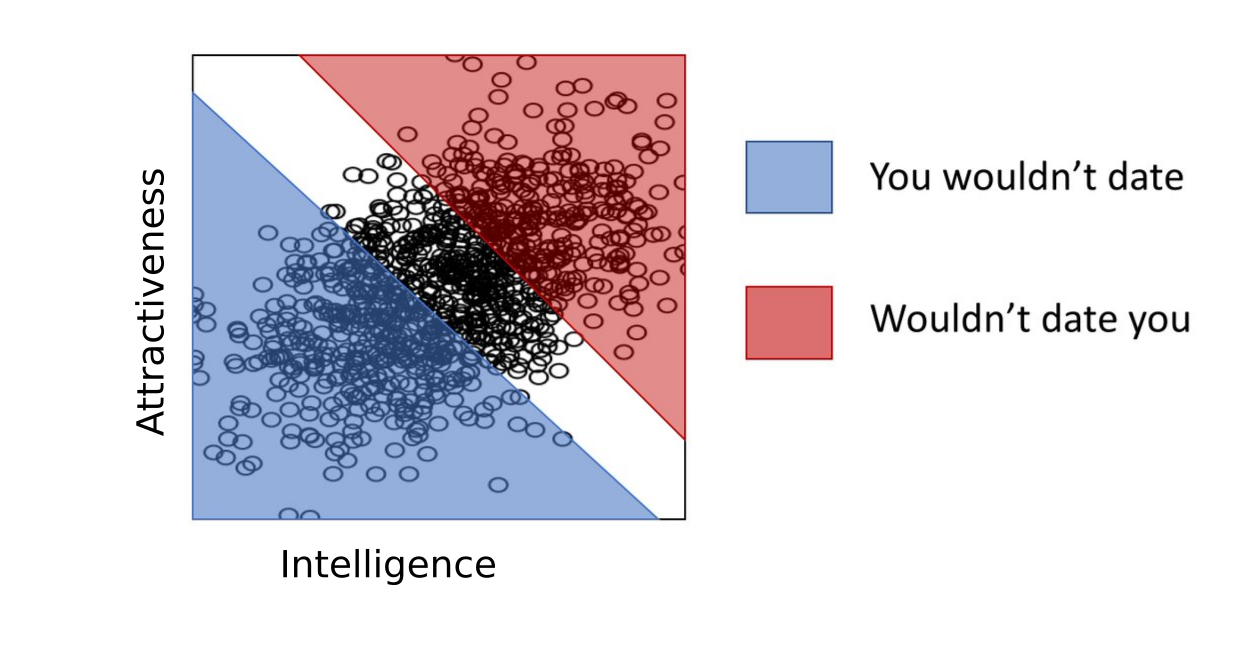
\includegraphics[width=5in]
{berkson/berkson.png}
\caption{
Example
of Berkson's paradox (BP).} 
\label{fig-berkson}
\end{figure}


Fig.\ref{fig-berkson}
presents an example
of BP. The
figure consists of
a scatter plot
with axes x=intelligence,
y=attractiveness, 
for a population of 
possible dates for a single person. 
For the full population,

\beq
(a,b)\sim P(a,b)=P(a)P(b)
\eeq
whereas for the population
in the white swath,

\beq
(a,b)\sim P(a,b|x)=P(b|a,x)P(a|x)\neq
P(b|x)P(a|x)
\;.
\eeq

As shown by
Fig.\ref{fig-berkson},
 BP is an example of {\bf selection bias}.
Selection bias happens when
a non-representative
subset of the total population
is considered (i.e., selected).



\chapter{Binary Decision Diagrams}\label{ch-binarydd}

\begin{figure}[h!]
$$
\begin{array}{c}
\xymatrix@C=.1pc{
&&&&&&&\stackrel{\rvA}{x_1?}\ar@{-->}[dllll]
\ar[drrrr]
\\
&&&\stackrel{\rvA_0}{x_2?}\ar@{-->}[dll]\ar[drr]
&&&&&&&&\stackrel{\rvA_1} {x_2?}\ar@{-->}[dll]\ar[drr]
\\
&\stackrel{\rvA_{00}}{ x_3?}\ar@{-->}[dl]\ar[dr]
&&&&\stackrel{\rvA_{01}} {x_3?}\ar@{-->}[dl]\ar[dr]
&&&&\stackrel{\rvA_{10}}{ x_3?}\ar@{-->}[dl]\ar[dr]
&&&&\stackrel{\rvA_{11}}{x_3?}\ar@{-->}[dl]\ar[dr]
\\
\rvA_{000}\ar[d]
&&\rvA_{001}\ar[d]
&&\rvA_{010}\ar[d]
&&\rvA_{011}\ar[d]
&&\rvA_{100}\ar[d]
&&\rvA_{101}\ar[d]
&&\rvA_{110}\ar[d]
&&\rvA_{111}\ar[d]
\\
\Rect{1}
&&\Rect{0}
&&\Rect{0}
&&\Rect{1}
&&\Rect{0}
&&\Rect{0}
&&\Rect{1}
&&\Rect{1}
}
\\
\begin{array}{ccc|l}
x_1&x_2&x_3&f(A_{x_1,x_2,x_2})
\\ \hline\hline
0
&0
&0
&1
\\ \hline
0
&0
&1
&0
\\ \hline
0
&1
&0
&0
\\ \hline
0
&1
&1
&1
\\ \hline
1
&0
&0
&0
\\ \hline
1
&0
&1
&0
\\ \hline
1
&1
&0
&1
\\ \hline
1
&1
&1
&1
\\ \hline
\end{array}
\end{array}
$$
\caption{Example of a binary tree and its truth table.
The truth table gives the values of $
f(x_1, x_2,x_3)=
\bar{x}_1(x_2+\bar{x}_3)  + x_1 x_2 $ }
\label{fig-bdd-tree}
\end{figure}

This chapter is based
on Wikipedia article Ref.\cite{wiki-bdd}
and other references.

A {\bf Binary Decision Diagram} (BDD) is a 
graph which represents 
in a more concise manner
the information in
a binary tree and
its accompanying truth table.

Fig.\ref{fig-bdd-tree} shows an
example of a binary tree and its 
truth table.
We will  convert this tree 
 into a BDD in this chapter. Each node asks a question with a binary (Boolean) answer. An answer of 0 (resp., 1 ) is indicated by a dashed (resp., full) arrow. The same question is asked by all nodes at the same level (i.e., depth) of the tree. In addition to the question, nodes are labeled uniquely by the random variable $\rvA_{x_1, x_2, \ldots, x_n}$,
where $n$ is the level of the node
and $x_i$ is the answer to the question $x_i?$.
The leaves of
the tree are square boxes that report 

\beq
f(x_1, x_2,x_3)=
\bar{x}_1(x_2+\bar{x}_3)  + x_1 x_2
\label{eq-bdd-truth-table}
\eeq
\begin{figure}[h!]
$$
\xymatrix@C=.1pc{
&&&&&&&x_1?\ar@{-->}[dllll]
\ar[drrrr]
\\
&&&x_2?\ar@{-->}[dll]\ar[drr]
&&&&&&&&x_2?\ar@{-->}[dll]\ar[drr]
\\
&x_3?\ar@{-->}[dl]\ar[dr]
&&&&x_3?\ar@{-->}[dl]\ar[dr]
&&&&x_3?\ar@{-->}[dl]\ar[dr]
&&&&x_3?\ar@{-->}[dl]\ar[dr]
\\
\Rect{1}
&&\Rect{0}
&&\Rect{0}
&&\Rect{1}
&&\Rect{0}
&&\Rect{0}
&&\Rect{1}
&&\Rect{1}
}
$$
\caption{The same tree as in Fig.\ref{fig-bdd-tree}, after dropping 
some labels that are not needed
for our discussion of BDDs.}
\label{fig-bdd-tree-simp}
\end{figure}


Fig.\ref{fig-bdd-tree-simp} shows
the same tree as in  Fig.\ref{fig-bdd-tree}, after dropping 
some labels that are not needed
for our discussion of BDDs.
Note that the {\bf question ordering} of the tree is
$x_1<x_2<x_3$. Other question
orderings such as $x_2< x_1 < x_3$
are possible. For a given
truth table, some question 
orderings lead to a BDD 
that has the full  
exponential complexity $2^n$
of the tree, where $n$ is 
the number of levels. Other question orderings
might lead to BDDs that have lower (such as linear in $n$) 
complexity.



\subsection{Conversion of Binary Tree into BDD}

A BDD is obtained
from a binary tree by 
successive application of the
following
3 rules:

\begin{enumerate}
\item Merge equivalent leaves (EL)
\item Merge isomorphic nodes (IN)
\item Eliminate parallel 0/1 arrows (PA) by merging source
and target nodes of the parallel  arrows.
\end{enumerate}

Fig.\ref{fig-el-pa-example} 
gives an example
of the application of rules EL and PA.
Fig.\ref{fig-example-in-rule}
gives an example of the 
application of the IN rule.


\begin{figure}[h!]
$$
\xymatrix{
\\\\
\stackrel{EL}{\implies}}
\xymatrix@C=.1pc{
&&&&&&&x_1?\ar@{-->}[dllll]
\ar[drrrr]
\\
&&&x_2?\ar@{-->}[dll]\ar[drr]
&&&&&&&&x_2?\ar@{-->}[dll]\ar[drr]
\\
&x_3?\ar@{-->}[drrrrrrr]\ar[drrrrr]
&&&&x_3?\ar@{-->}[dr]\ar[drrr]
&&&&x_3?\ar@{-->}[dlll]\ar@/_1pc/[dlll]
&&&&x_3?\ar@{-->}[dlllll]\ar@/_1pc/[dlllll]
\\
&&
&&
&&\Rect{0}
&&\Rect{1}
&&
&&
&&
}
\xymatrix{
\\\\\stackrel{PA}{\implies}}
\xymatrix@C=.1pc{
&&&&&&x_1?\ar@{-->}[dllll]
\ar[d]
\\
&&x_2?\ar@{-->}[dll]\ar[drr]
&&&&x_2?\ar@{-->}[ddll]\ar[dd]
\\
x_3?\ar@{-->}[drrrrrr]\ar[drrrr]
&&&&x_3?\ar@{-->}[d]\ar[drr]
\\
&&
&&\Rect{0}
&&\Rect{1}
&&
&&
&&
}
$$
\caption{This is the 
result of applying the
the EL rule, followed by the PA
rule, to Fig.\ref{fig-bdd-tree-simp}.}
\label{fig-el-pa-example}
\end{figure}

\begin{figure}[h!]
$$
\begin{array}{c}
\xymatrix@C=.1pc{
&&&&&&x_1?\ar@{-->}[dllll]
\ar[drrr]
\\
&&x_2?\ar@{-->}[dll]\ar[drr]
&&&&&&&x_2?\ar@{-->}[ddlllll]\ar[ddlll]
\\
x_3?\ar[drrrrrr]\ar@{-->}[drrrr]
&&&&x_3?\ar@{-->}[d]\ar[drr]
\\
&&
&&\Rect{0}
&&\Rect{1}
&&
&&
&&
}
\xymatrix{\\\\
\stackrel{IN}{\implies}}
\xymatrix@C=.1pc{
&&&&&&x_1?\ar@{-->}[dllll]
\ar[drrr]
\\
&&x_2?\ar@{-->}[dll]\ar@/_1pc/[dll]
&&&&&&&x_2?\ar@{-->}[ddlllll]\ar[ddlll]
\\
x_3?\ar[drrrrrr]\ar@{-->}[drrrr]
&&&&
\\
&&
&&\Rect{0}
&&\Rect{1}
&&
&&
&&
}
\\
\xymatrix{\\\\\stackrel{PA}{\implies}}
\xymatrix@C=.1pc{
&x_1?\ar@{-->}[dl]\ar[dr]
\\
x_2?\ar@{-->}[d]\ar[drr]
&&x_2?\ar[d]\ar@{-->}[dll]
\\
\Rect{0}
&&\Rect{1}
}
\xymatrix{\\\\\stackrel{IN}{\implies}}
\xymatrix@C=.1pc{x_1?\ar@{-->}[d]\ar@/_1pc/[d]
\\
x_2?\ar@{-->}[d]\ar[dr]
\\
\Rect{0}
&\Rect{1}
}
\xymatrix{\\\\\stackrel{PA}{\implies}}
\xymatrix@C=.1pc{
\\
x_1?\ar@{-->}[d]\ar[dr]
\\
\Rect{0}
&\Rect{1}
}\end{array}
$$
\caption{An example 
to illustrate the application of the
IN rule}
\label{fig-example-in-rule}
\end{figure}





\section{Equivalent Bnet}

\begin{figure}[h!]
$$
\begin{array}{cc}
\xymatrix@C=.1pc{
&&&&&&&x_1?\ar@{-->}[dllll]
\ar[dr]
\\
&&&x_2?\ar@{-->}[dll]\ar[drr]
&&&&&x_2?\ar@{-->}[ddll]\ar[dd]
\\
&x_3?\ar@{-->}[drrrrrrr]\ar[drrrrr]
&&&&x_3?\ar@{-->}[dr]\ar[drrr]
\\
&&
&&
&&\Rect{0}
&&\Rect{1}
&&
&&
&&
}
&
\xymatrix@C=.1pc{
&&&&&&&\Circle{\rva, x_1?}\ar@{-->}[dllll]|{\ol{x_1}}
\ar[dr]|{x_1}
\\
&&&\Circle{\rvb, x_2?}\ar@{-->}[dll]|{\ol{x_2}}\ar[drr]|{x_2}
&&&&&\Circle{\rvc, x_2?}\ar[dd]|{x_2}
\\
&\Circle{\rvd, x_3?}\ar@{-->}[drrrrrrr]|{\ol{x_3}}
&&&&\Circle{\rve, x_3?}\ar[drrr]|{x_3}
\\
&&
&&
&&
&&\Rect{\ul{y}}
&&
&&
&&
}
\\
(a) & (b)
\end{array}
$$
\caption{
$(a)$ 
is the BDD 
at the end of the
conversion chain in  Fig.\ref{fig-el-pa-example}.
$(b)$ 
is a LD (Linear Deterministic) bnet that
is equivalent to the BDD of
$(a)$. $(b)$ is
obtained by keeping a subset of the arrows in $(a)$. The remaining
arrows are given gain $x_i$
(resp., $\bar{x}_i$) if they are full 
(resp., dashed) and originate from
a node with question $x_i?$.
}
\label{fig-bdd-to-bnet}
\end{figure}




In Fig.\ref{fig-bdd-to-bnet}, $(a)$
is a BDD and 
$(b)$ is a LD (Linear Deterministic) bnet equivalent to $(a)$.
The structural equations of the LD bnet, printed in blue,
are as follows:

\beq\color{blue}
\rvy=  x_2 \rvc + x_3 \rve + \bar{x}_3\rvd
\eeq

\beq\color{blue}
\rvd=\bar{x}_2\rvb
\eeq

\beq\color{blue}
\rve=x_2\rvb
\eeq

\beq\color{blue}
\rvb = \bar{x}_1\rva
\eeq

\beq\color{blue}
\rvc=x_1\rva
\eeq
Therefore

\beq
\rvy = [\bar{x}_1(x_2 x_3 +\bar{x}_2\bar{x}_3)
+ x_1 x_2
]\rva
\label{eq-3-histories-coeff}
\eeq

The equivalence of $(a)$ and $(b)$
follows from the following transformation
of Eq.(\ref{eq-bdd-truth-table})

\begin{align}
f(x_1, x_2,x_3) =&
\bar{x}_1(x_2+\bar{x}_3)  + x_1 x_2
\\
=&
\bar{x}_1[x_2(x_3+\bar{x}_3)+\bar{x}_3
(x_2+ \bar{x}_2)]  + x_1 x_2
\;\text{(because $x+\bar{x}=1$ in base 2)}
\\
=&
\bar{x}_1[x_2(x_3)+\bar{x}_3
(\bar{x}_2)]  + x_1 x_2\;, \text{
(because $2x_2\bar{x}_3=0$ in base 2)
}
\label{eq-bdd-truth-table-equiv}
\end{align}
Note that the right 
hand side of Eq.(\ref{eq-bdd-truth-table-equiv})
gives the same 3 \qt{Feynman histories}
as the coefficient of $\rva$ in
 Eq.(\ref{eq-3-histories-coeff}).

\begin{figure}[h!]
$$
\begin{array}{ccc}
\xymatrix{
\Circle{\rva}
\ar[d]|{x_1}
\\
\Circle{\rvb}
\ar[d]|{x_2}
\\
\Circle{\rvc}
}
&\;\;\;&
\xymatrix{
&\Circle{\rva}\ar[dl]|1
\ar[dr]|1
\\
\Circle{\rvb}\ar[dr]|{x_1}
&&\Circle{\rvc}\ar[dl]|{x_2}
\\
&\Circle{\rvd}
}
\\
\rvc=x_2\rvb=x_2x_1\rva
&&
\rvc= (x_1 + x_2)\rva
\end{array}
$$
\caption{Expressing the sum or product 
of two boolean variables $x_1$, $x_2$ 
as a LD bnet}
\label{fig-bdd-and-or}
\end{figure}

It's easy to  express the sum or product 
of two boolean variables $x_1$, $x_2$ 
as a LD bnet.
(see Fig.\ref{fig-bdd-and-or})
In general, any boolean polynomial
can be expressed as a LD bnet. In particular, the sum of products and product of sums
canonical forms
of any boolean expression can be expressed 
thus.
\chapter{Chow-Liu Trees
and Tree Augmented Naive Bayes (TAN)}

This chapter is mostly based
on chapter 8 of Pearl's 1988 book
Ref.\cite{pearl-1988book}. See also 
Ref.\cite{wiki-chow} and references
therein.

This chapter uses various Shannon Information Theory
entropies. Our 
notation for these
entropies
is described in Chapter \ref{ch-not-cons}
on Notational Conventions.


Chow-Liu trees refers 
to an 
algorithm for finding
a bnet tree
that fits an a priori
given probability distribution
as closely as possible.


Consider a bnet with $n$ nodes
$\rvx^n=(\rvx_0, \rvx_1, \ldots, \rvx_{n-1})$
such that 
$\rvx_i\in S_{\rvx_i}$
for all $i$. Let its  
 total probability distribution be
$P_{\rvx^n}$. For
simplicity, we will abbreviate $P_{\rvx^n}$ by $P$.
Hence


\beq
P(x^n)=P_{\rvx^n}(x^n)
\;.
\eeq

Suppose we want to fit $P_{\rvx^n}$
by a tree bnet with nodes
$\rvt^n=(\rvt_0, \rvt_1, \ldots, \rvt_{n-1})$
such that
$\rvt_i\in S_{\rvt_i}=S_{\rvx_i}$
for all $i$.
 For
simplicity, we will abbreviate $P_{\rvt^n}$ by $P_T$.
Hence

\beq
P_T(x^n)=P_{\rvt^n}(x^n)
\;.
\eeq

Throughout this chapter, let
$V=\{0, 1, \ldots, n-1\}$, the set of vertices.
Suppose $\mu$ is a function
$\mu:V\rarrow V$
such that $\mu(i)< i$.
Let
$T_\mu=\{\rvt_{\mu(i)}\rarrow \rvt_i:
 i\in V-\{0\}\}$.
Then $T_\mu$
is a tree that spans (
i.e., it includes all nodes)
 $\rvt^n$.
Its root node 
is
$\rvt_0$, because $\rvt_0$ has no parents.
All other nodes $\rvt_i$ have exactly
one parent,
namely $ \rvt_{\mu(i)}$.
Let $P_T$,
the total probability 
distribution for 
the tree, be parameterized
by the function $\mu$
as follows:



\beq
P_T(x^n)=\prod_{i=0}^{n-1}
P_T(x_i|x_{\mu(i)})
\label{eq-pt-prod}
\;,
\eeq
where, for the root node 0, 
$P_T(x_0|x_{\mu(0)})=P_T(x_0)$.

\begin{claim}\label{claim-chow1}
$D_{KL}(P\parallel P_T)$
is minimized 
over all
probability
distributions
$P_T$ that are
expressible as 
Eq.(\ref{eq-pt-prod})
iff

\beq
P_T(x_i|x_{\mu(i)})
=
P(x_i|x_{\mu(i)})
\eeq
for all $i$, and

\beq
\sum_i H(\rvx_i:\rvx_{\mu(i)})
\eeq
is maximized over all $\mu$.
\end{claim}
\proof

\beqa
D_{KL}(P\parallel P_T)
&=&
\sum_{x^n} P(x^n)\ln 
\frac{P(x^n)}{P_T(x^n)}
\\
&=&
-\sum_{x^n}
\sum_i P(x^n)\ln 
P_T(x_i| x_{\mu(i)})
+
\sum_i P(x^n)\ln 
P(x^n)
\\
&=&
-
\sum_i
\sum_{x_i, x_{\mu(i)}} P(x_i, x_{\mu(i)})\ln 
P_T(x_i| x_{\mu(i)})
-
H(\rvx^n)
\\
&=&
-
\sum_i
\sum_{x_{\mu(i)}} 
P(x_{\mu(i)})
\left[
\sum_{x_i}
P(x_i| x_{\mu(i)})\ln 
P_T(x_i| x_{\mu(i)})
\right]
-
H(\rvx^n)
\;.
\eeqa
Now note that

\beq
\sum_{x_i}
P(x_i| x_{\mu(i)})\ln 
\frac
{P(x_i| x_{\mu(i)})}
{P_T(x_i| x_{\mu(i)})}
\geq 0
\eeq
and
this inequality
becomes an equality iff

\beq
P(x_i| x_{\mu(i)})=
P_T(x_i| x_{\mu(i)})
\;.
\label{eq-inherits-tpm}
\eeq
Therefore

\beq
D_{KL}(P\parallel P_T)
\geq
-
\sum_i
\underbrace{
\sum_{x_{\mu(i)}} 
P(x_{\mu(i)})
\left[
\sum_{x_i}
P(x_i| x_{\mu(i)})\ln 
P(x_i| x_{\mu(i)})
\right]
}_{=H(\rvx_i|\rvx_{\mu(i)})=
H(\rvx_i:\rvx_{\mu(i)})-H(\rvx_i)}
-
H(\rvx^n)
\;,
\eeq
and this inequality
becomes an equality iff
Eq.(\ref{eq-inherits-tpm})
is satisfied.

Note from the last
equation that

\beq
\argmin_\mu D_{KL}(P\parallel P_T)=
\argmax_\mu
\sum_i H(\rvx_i:\rvx_{\mu(i)})
\;.
\eeq
\qed


\begin{claim}\label{claim-chow2}
\beq
\argmin_\mu H(\rvx^n)
=
\argmax_\mu \sum_i H(\rvx_i:\rvx_{\mu(i)})
\eeq
\end{claim}
\proof
\beqa
H(\rvx^n)&=&
-\sum_{x^n}P(x^n)\sum_i\ln P(x_i|x_{\mu(i)})
\\
&=&
-\sum_i
\sum_{x_i, x_{\mu(i)}} 
P(x_i, x_{\mu(i)})\ln 
P(x_i| x_{\mu(i)})
\\
&=&
-\sum_i
\sum_{x_i, x_{\mu(i)}} 
P(x_i, x_{\mu(i)})
\left[\ln \frac
{P(x_i| x_{\mu(i)})}
{P(x_i)}
+\ln P(x_i)
\right]
\\
&=&
-\sum_i
\left[
H(\rvx_i:\rvx_{\mu(i)})
-
H(\rvx_i)
\right]
\\
&=&
\sum_i H(\rvx_i)
-
\sum_i H(\rvx_i:\rvx_{\mu(i)})
\eeqa
\qed

The meaning 
of Claims \ref{claim-chow1}
and \ref{claim-chow2} 
is as follows. If
$D_{KL}(P\parallel P_T)$
is minimized over all $P_T$, then
\begin{enumerate}
\item$P_T$
inherits
its TPM's 
from $P$, and
\item
$P_T$ gets
its structure,
which is being parameterized
by 
the function $\mu$,
by
maximizing 
the score given by 

\beq
\text{score}
=\sum_i H(\rvx_i:\rvx_{\mu(i)})
\;.
\eeq
(mutual information
$H(\rva:\rvb)$
measures
correlation
between $\rva$ and $\rvb$).
Maximizing the score
is the same
as minimizing the entropy
$H(\rvx^n)$
over all the
structures  $\mu$.
(i.e., 
finding least complex structure).
\end{enumerate}

So far,
we have
studied the properties
of those 
probability 
distributions
$P_T$
for a tree bnet
that 
best
approximates
an a priori given
probability
distribution $P$,
but
we haven't yet
described
how to 
build a Chow-Liu tree
based on
empirical data.
Next we give
Chow-Liu's algorithm
for doing so.


\begin{enumerate}
\item {\bf Find MST using Kruskal's 
algorithm\footnote{Kruskal's algorithm is 
one several famous algorithms (Prim's
algo is another one) for
finding an MST (maximum or
minimum spanning tree).  
An MST algorithm
 takes an
undirected graph 
with
weights along its edges as input.
It then
 finds a tree subgraph (i.e., subset
of the edges of the graph
with no loops) that
(1) spans the graph
(i.e., includes every vertex
of the graph) and (2)
maximizes (or
minimizes)
the
 sum of weights among all possible
 tree subgraphs.
For more information,
see Ref\cite{wiki-spanning-tree} and references
therein, or any other
of numerous explanations
of MST in the Internet.}.
(see Fig.\ref{fig-spanning-tree})}\\
Calculate weights $w_{i, j}=
H(\rvx_i:\rvx_j)$ for all
$i, j\in V$  and store them 
in a dictionary
 $D$
that maps edges to weights.\\
Order $D$ by weight size.\\
Let $T$ be a list of the edges in the tree. 
Initialize $T$ to  empty.\\
Repeat this until $T$ has $n-1$ elements:\\
\hspace*{1cm}Remove largest weight $w$ from $D$
and corresponding edge $e$.\\
\hspace*{1cm}Add $e$ to $T$ if $\{e\}\cup T$
has no loops. Otherwise discard $e$ and $w$.

\item{\bf  Give directions to edges in $T$.
(see Fig.\ref{fig-tree-dir})}\\
Let $DT$ be a list of directed edges.
Initialize $DT$ to empty.\\
Choose any node as root node.\\
Point arrows along edges in $T$,
away 
from root node.\\
Add new arrows to $DT$.\\ 
Repeat this until $DT$ has $n-1$ elements:\\
\hspace*{1cm}Point arrows
along edges in $T$,
away from 
leaf nodes of current  $DT$.\\
\hspace*{1cm}Add new arrows to $DT$.
\end{enumerate}

\begin{figure}[h!]
\centering
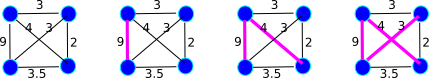
\includegraphics[width=5in]
{chow/spanning-tree.png}
\caption{
Example of finding MST (maximum spanning tree)} 
\label{fig-spanning-tree}
\end{figure}

\begin{figure}[h!]
\centering
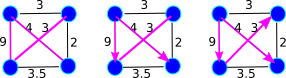
\includegraphics[width=3in]
{chow/tree-dir.png}
\caption{Example of giving directions
to edges of spanning tree.} 
\label{fig-tree-dir}
\end{figure}

Nodes in a Chow-Liu tree can
be rated in
terms
of their relative importance.
Here are 2 possible
metrics
for measuring 
the importance
of a node $\rva$:

\beq
N_{nb}(\rva)=
\text{ number of neighbors of $\rva$}
\eeq

\beq
{\rm traffic}(\rva)=
\sum_{\rvn\in nb(\rva)}
H(\rva:\rvn)
\eeq
For example,
to get a tree with low depth, 
one can choose
as the root node
the node which has 
largest $N_{nb}$, and
if there are several
with the same largest $N_{nb}$,
choose out of those the 
one with the largest traffic.


\section*{Tree Augmented Naive Bayes (TAN)}

Recall from Chapter \ref{ch-naive}
that a Naive
Bayes bnet
consists
of  a class node $\rvc$
with
$n$ children nodes
$\rvx^n$, called the feature nodes. A
Tree Augmented Naive Bayes (TAN) bnet
is a Naive Bayes bnet with 
a 
tree grafted onto it like a chimera.
More precisely,
one starts
with a Naive Bayes bnet 
and adds arrows between
the feature nodes.
The arrows are added in such a way
that the TAN bnet sans node $\rvc$
constitutes a tree.
It's not the most well 
motivated bnet in human
history,
but at least
it adds a bit
of correlation between
the feature nodes
of the Naive Bayes bnet.
Those nodes are independent
at fixed $\rvc$
in the Naive Bayes
bnet, but are no longer so
in the TAN bnet.
See Figs.\ref{fig-naive-tree}
and \ref{fig-tan}
for an example of a TAN bnet.



\begin{figure}[h!]
\centering
$$\xymatrix{
\rvc\ar[d]\ar[dr]\ar[drr]\ar[drrr]\\
\rvx_0&\rvx_1&\rvx_2&\rvx_3
}
\;\;\;\;
\xymatrix{
\rvx_0&\rvx_1
&\rvx_2\ar[l]\ar@/^1pc/[ll]
&\rvx_3\ar[l]
}$$
\caption{bnet for Naive Bayes
with 4 feature nodes
and another bnet for a tree
made of the same feature nodes.}
\label{fig-naive-tree}
\end{figure}

\begin{figure}[h!]
\centering
$$\xymatrix{
\rvc\ar[d]\ar[dr]\ar[drr]\ar[drrr]\\
\rvx_0&\rvx_1
&\rvx_2\ar[l]\ar@/^1pc/[ll]
&\rvx_3\ar[l]
}$$
\caption{
TAN bnet constructed
by merging Naive
Bayes bnet
and tree
bnet
of Fig.\ref{fig-naive-tree}.}
\label{fig-tan}
\end{figure}


The total probability distribution
$P_{TAN}$ for a TAN bnet
can be parameterized as follows.

\beq
P_{TAN}(x^n, c)=P_{TAN}(c)\prod_{i=0}^{n-1}
P_{TAN}(x_i|x_{\mu(i)}, c)
\;.
\eeq

As with Chow Liu trees,
we can attempt
to find a TAN bnet
whose total 
probability $P_{TAN}=P_{\rvt^n, \rvc}$
best approximates
an a priori given probability 
distribution $P=P_{\rvx^n, \rvc}$.

Note that
\begin{claim}

\beq
\argmin_\mu H(\rvx^n, \rvc)
=
\argmax_\mu
\sum_i H(\rvx_i:\rvx_{\mu(i)}| \rvc)
\eeq
\end{claim}
\proof

\beqa
H(\rvx^n, \rvc)
&=&-
\sum_{x^n,c}P(x^n,c)
\left[
\ln P(c)+
\sum_i
\ln P(x_i|x_{\mu(i)}, c)
\right]
\\
&=&-
\sum_{x^n,c}P(x^n,c)
\left[
\ln P(c)+
\sum_i
\ln \left(\frac{P(x_i, x_{\mu(i)}|c)}
{P(x_i|c)P(x_{\mu(x_i)}|c)}
P(x_i| c)
\right)
\right]
\\
&=&
\sum_i H(\rvx_i, \rvc)
-
\sum_i H(\rvx_i:\rvx_{\mu(i)}|\rvc)
\eeqa 
\qed


Following
the same line of
reasoning
that we followed
for Chow-Liu trees,
we conclude that:

If $D_{KL}(P\parallel P_{TAN})$
is minimized over all $P_{TAN}$, then
\begin{enumerate}
\item$P_{TAN}$
inherits
its TPM's 
from $P$, and
\item
$P_{TAN}$ gets
its structure,
which is being parameterized
by 
the function $\mu$,
by
maximizing 
the score defined by

\beq
\text{score}
=\sum_i H(\rvx_i:\rvx_{\mu(i)}|\rvc)
\label{eq-score-tan}
\eeq
\end{enumerate}

One can build a TAN bnet
from empirical data as follows:

Calculate a Chow-Liu Tree
for each $c\in S_\rvc$.
For each of those trees,
create a TAN bnet, and 
calculate its
score given by
  Eq.(\ref{eq-score-tan}).
Keep
the TAN bnet with
the largest score.


\chapter{Counterfactual Reasoning}
\label{ch-counterf}


\section{The 3 Rungs of Causal AI}
According to 
Judea Pearl,
there are 3 rungs in the
ladder of causal AI.
These are (as I see them):
\begin{enumerate}
\item
{\bf Observing Passively:} Collecting 
data
and fitting curves to it,
without any plan 
designed to
investigate Nature's 
causal connections.
\item {\bf Doing causal
experiments:} 
Doing experiments 
consciously designed to
elucidate
Nature's causal connections.
Even cats do this!, but current AI doesn't.
\item {\bf Imagining
 counterfactual situations, Analogizing:}
Imagining gedanken experiments
to further understand
Nature's causal connections,
and to decide what future
courses of action are
more likely to succeed,
even if
those courses of action
are unprecedented, and have never been taken before.
Making
predictions about
 events that have never happened (``counterfactuals")
is a very Bayesian
concern, well out of the purview of 
frequentists. Nevertheless,
humans do such
``analogizing" 
all the time to great advantage.
It becomes
possible if there
is some indirect but similar
data that can be transported
(transplanted, applied)
to the situation of
interest.
\end{enumerate}
Chapter \ref{ch-mpass}
on message passing
is about rung 1.
Chapter \ref{ch-do-calc}
on Do Calculus is about rung 2.
This chapter is dedicated to rung 3.

Judea Pearl 
is fond of discussing rung 3 solely
in terms of SCM.\footnote{SCM are 
what we call DEN. DEN (deterministic systems
with external noise) are discussed in
Chapter \ref{ch-linear-sys}. }
In this chapter,
we define rung 3
without using SCM, using solely
bnets.
This gives a more general
version of rung 3,
because SCM are a subset of bnets.



We will use the
term {\bf intervention operator (or simply ``intervention")} 
to refer to an operator
that maps a bnet to another bnet.
In Chapter \ref{ch-do-calc},
we introduced an intervention operator
 called the {\bf do operator}
$\cald_{\rvx=x}$ (this is our notation for what Pearl 
symbolizes by $do(\rvx)=x$).
The study of counterfactuals 
requires that we
introduce a new
kind of intervention 
operator that we will
call an {\bf imagine operator},
and denote by $\cali_{\rvx\rarrow\rvy}(\tilde{x})$.
These 2 types of interventions 
will be defined 
next.

\section{Do operator}


\begin{figure}[h!]
\centering
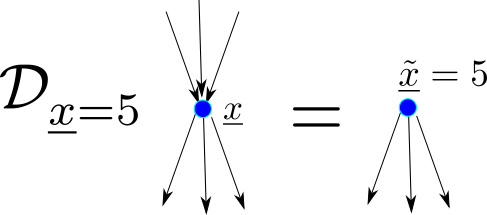
\includegraphics[width=1.75in]
{counterf/rho-op.png}
\caption{Action
of ``do" operator $\cald_{\rvx=5}$
on node $\rvx$.} 
\label{fig-rho-op}
\end{figure}

The do operator $\cald_{\rvx=5}$
is defined graphically in Fig.\ref{fig-rho-op}.
The TPM, printed in blue,
 for node $\tilde{\rvx}$ of Fig.\ref{fig-rho-op},
is given by

\beq\color{blue}
P(\tilde{x})=\delta(5, \tilde{x})
\eeq


The do operator $\cald_{\rvx=5}$
amputates
the incoming arrows of node $\rvx$
and sets the TPM
of the new root node $\tilde{\rvx}$
to a delta function $\delta(
\tilde{x}, 5)$
(or some state of $\rvx$
 other than 5).
Sometimes we call the new node
$\cald\rvx$
instead of 
$\tilde{\rvx}$.

The uses of the do operator are discussed
in detail in Chapter \ref{ch-do-calc}.

\section{Imagine operator}

\begin{figure}[h!]
\centering
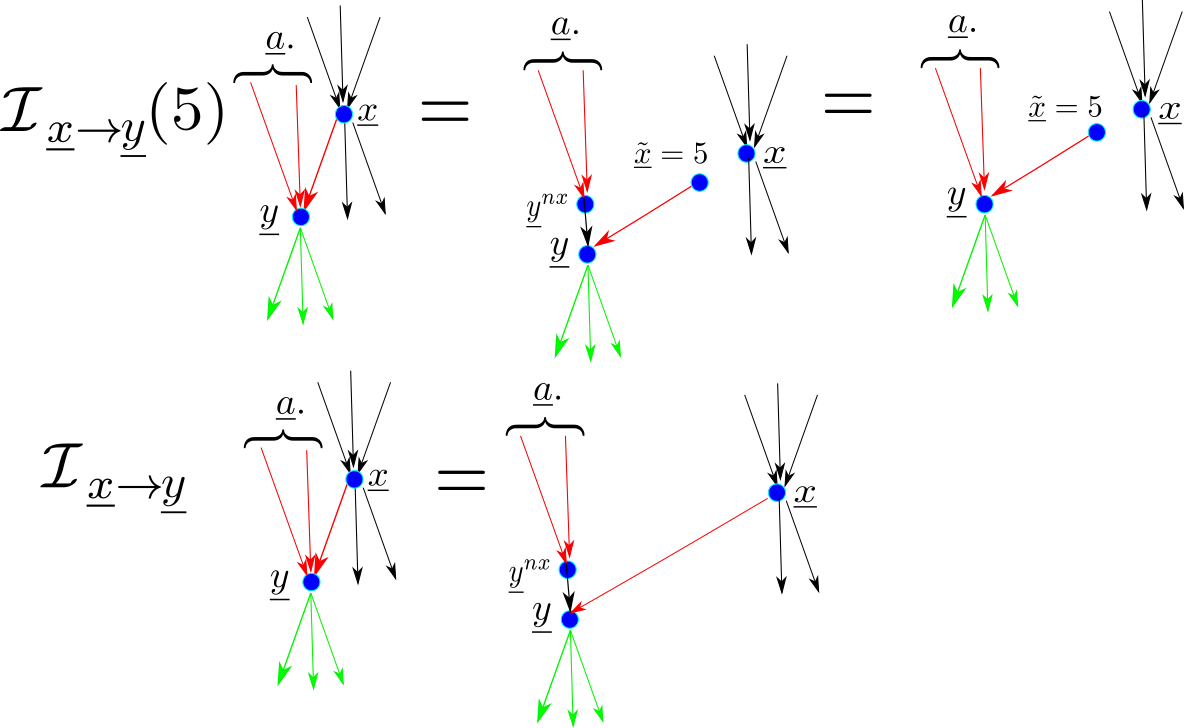
\includegraphics[width=4in]
{counterf/kappa.png}
\caption{Action of ``imagine" operators 
$\cali_{\rvx\rarrow \rvy}(5)$
and $\cali_{\rvx\rarrow \rvy}$
on arrow $\rvx\rarrow \rvy$.
In this figure, $y^{nx}=[y(x)]_{\forall x\in S_\rvx}$,
where $nx=|S_\rvx|$
and $S_\rvx$ is the set of states of node $\rvx$.
} 
\label{fig-kappa}
\end{figure}

The imagine operator  $\cali_{\rvx\rarrow \rvy}(5)$
is defined graphically in Fig.\ref{fig-kappa}.
Note that Fig.\ref{fig-kappa}
actually defines two types 
of imagine operators, the one
with an argument:
$\cali_{\rvx\rarrow \rvy}(5)$,
and the one without an argument: 
$\cali_{\rvx\rarrow \rvy}$.
The TPMs, printed in blue, 
for various nodes in
Fig.\ref{fig-kappa}, are as follows.



\begin{itemize}

\item
For $\cali_{\rvx\rarrow 
\rvy}(\tilde{x})G$

\beq\color{blue}
P(y| \tilde{x}, a.)=
P(y| \rvx=\tilde{x}, a.)
\eeq

\beq\color{blue}
P(\tilde{x})=
\delta(\tilde{x}, 5)
\eeq

\item
For $\cali_{\rvx\rarrow \rvy}G$
\beq\color{blue}
P(y^{nx}| a.)=\prod_{\tilde{x}}
P(\rvy(\tilde{x})=y(\tilde{x})|a.)
\eeq

\beq\color{blue}
P(y|y^{nx}, x)=
\delta(y,y(x))
\eeq
\end{itemize}
The imagine operators 
$\cali_{\rvx\rarrow\rvy}(5)$
and $\cali_{\rvx\rarrow\rvy}$
operate on an arrow
whereas the 
$\cald$ operator
 operates on a node.
$\cali_{\rvx\rarrow\rvy}(5)$
deletes
arrow $\rvx\rarrow\rvy$
and
creates a new root node 
$\tilde{\rvx}$
and a new arrow
$\tilde{\rvx}\rarrow \rvy$.
Sometimes we call
the new node
$\cali_\rvy\rvx$
instead of
 $\tilde{\rvx}$. 
$\cali_{\rvx\rarrow\rvy}$
creates 
a new node $\rvy^{nx}$
and an arrow $\rvy^{nx}\rarrow \rvy$.



\begin{figure}[h!]
$$
\begin{array}{ccccc}
\xymatrix{
&\rvx\ar@[red][ddr]\ar[ddl]
\\
&&&
\\
\rvd\ar@[red][rr]
&
&\rvy\ar@[green][r]
\ar@[green][ur]
&
}
&
\xymatrix{
&&\rvx\ar[ddll]\ar@[red][d]
\\
&&[\rvy(0),\rvy(1)]\ar[d]
&
\\
\rvd\ar@[red][rr]
&
&\rvy\ar@[green][r]
\ar@[green][ur]
&
}
\\
\\
G&G_+=\cali_{\rvd\rarrow\rvy}G
\end{array}
$$
\caption{How 
 imagine operator 
arises in 
Potential Outcomes (PO)
theory.
} 
\label{fig-counterf-G-im-y0-y1}
\end{figure}
Fig.\ref{fig-counterf-G-im-y0-y1}
shows how the
imagine operator arises
in Potential Outcomes (PO) theory.
PO theory is discussed extensively
in Chapter \ref{ch-pot-out}.
As you can see, PO theory
only uses a limited version
of the 3 rungs
of causal inference, because it 
doesn't use the do-operator,
and it only uses one 
of 2 possible types of
imagine operators.
Furthermore,
it assumes a
very limited triangular DAG.


\begin{figure}[h!]
\centering
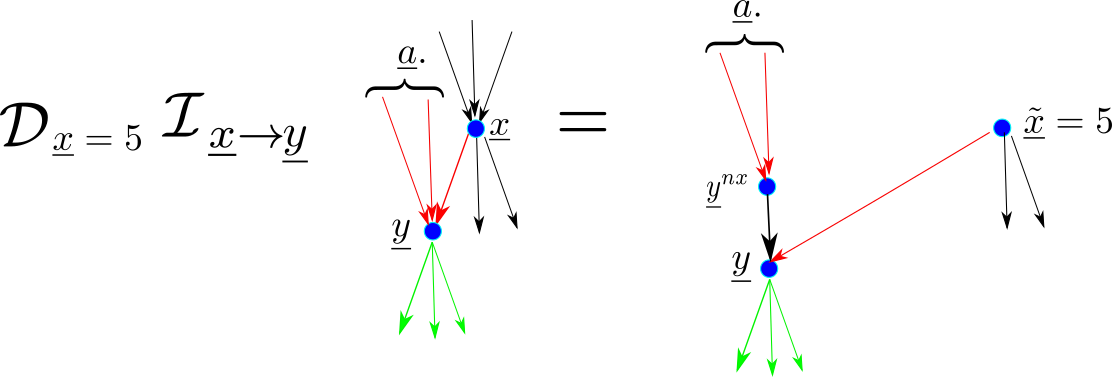
\includegraphics[width=3.5in]
{counterf/rho-kappa.png}
\caption{$\cald_{\rvx=5}\cali_{\rvx\rarrow \rvy}G$
gives a connection
between do and imagine operators.
} 
\label{fig-rho-kappa}
\end{figure}

Fig.\ref{fig-rho-kappa}
gives  a connection
between do and imagine
operators.
We see
from that figure that
for $\cald_{\rvx=\tilde{x}}
\cali_{\rvx\rarrow\rvy}G$, we have\footnote{In the
notation favored by Pearl, Eq.(\ref{eq-connect-do-imag})
 would be
$$P(y|do(X)=\tilde{x}, a.)=P(Y_{\tilde{x}}=y|a.)$$}
\beq
P(y|\cald\rvx=\tilde{x}, a.)=P(\rvy(\tilde{x})=y|a.)
\label{eq-connect-do-imag}
\eeq


One can define
a {\bf do-imagine-calculus}
whose
objective
is to 
express
probabilities such as 
$P(\rvy|\cald\rvr=r,
\cali_\rvb \rvs=s, t)$
in terms of observable 
probabilities
that do not
contain
any do or imagine
operators in them.
As with
Do Calculus,
this reduction
is not 
always possible,
and we say a probability is
{\bf $\cald$-identifiable},
{\bf $\cali$-identifiable}
or
{\bf $\cald\cali$-identifiable}
if it  can be 
expressed without do, imagine
or both operators.


\chapter{Cross-Validation}
\label{ch-cross-val}

This chapter is based on Ref.\cite{wiki-xval}.

Cross-Validation (CV)
is a method 
of calculating the 
{\bf ``out-of-training-set" (OOTS) error}
for a classifier.
What this means is that the classifier 
is trained on a training set,
and its propensity to err is evaluated
on a set different from the training set.

In {\bf $k$-fold CV}, the most common CV method, 
and the only one we will discuss in this chapter,
one
partitions a  
dataset into $k$ disjoint datasets
of equal length.
One uses $k-1$ of those
sub-datasets to train a model,
and saves the last sub-dataset to
validate the model just trained.
One actually rotates which of 
the $k$ sub-datasets is used 
for validation purposes,
and calculates $k$ validation 
errors $\cale_j$ for $j=0, 1, \ldots, k-1$.
Then one averages over the $\cale_j$
to obtain a final OOTS error $\cale$. 

CV strongly resembles
Jackknife
Resampling (JR) 
(see Chapter \ref{ch-jack}),
but in JR 
the validation sub-dataset is
never used for anything,
whereas in CV,
it is used for validation
purposes, to calculate
an OOTS error.

Next, we will
explain $k$-fold CV more explicitly,
using 
equations and a bnet.


Let $L=[0,1,2, \ldots, nsam-1]$ be a list of
individuals (samples) in a population.
In this chapter, we will use the notation 
$A^\s=A[\s]$ 
and $\vec{A}=[A^\s:\s\in L]$
for a  list (vector, 1-D  array) indexed by $L$.
We will refer to $DS=(\vec{x}, \vec{y})$ 
where $x^\s\in S_\rvx$, $y^\s\in S_\rvy$,
as a dataset.
If
$L_j$ is a list (possibly with 
duplicate items)
such that $set(L_j)\subset set(L)$, then
define
$DS_j=(\vec{x}, \vec{y})_{L_j}=
((x^\s)_{\s\in L_j}, 
(y^\s)_{\s\in L_j})$.

Let
$J=\{0,1, 2, \ldots, nj-1\}$.

Define a {\bf training list(TL),
validation list(VL) pair} $(TL,VL)$
to be a pair of lists
such that 
$set(TL)$ and $set(VL)$
are disjoint subsets
of $set(L)$.
Let $(TL_j, VL_j)$ for $j\in J$
be $nj$ such TL-VL pairs.


Fig.\ref{fig-xfold-xval} 
shows
the TL-VL pairs 
that are used
when doing $k$-fold 
CV.
In that figure, $k=nj=4$.
As you can see,
in $k$-fold CV, one chooses 
$nj=k$ list pairs $(TL_j, VL_j)$
such that all individuals $\s\in L$
appear exactly once, in either
$TL_j$ or $TV_j$, but not in both.

\begin{figure}[h!]
\centering
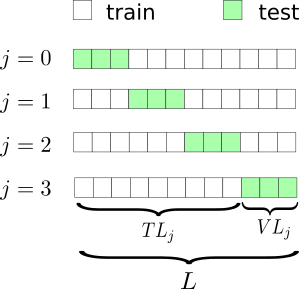
\includegraphics[width=2in]
{cross-val/kfold-xval.png}
\caption{4-fold CV with $|L|=12$.
For all $j$,
$|VL_j|=3$ and $|TL_j|=9$. 
All individuals $\s\in L$
appear exactly once, in either
$TL_j$ or $TV_j$, but not in both.} 
\label{fig-xfold-xval}
\end{figure}

We will refer to a function
$Y:S_\rvx \rarrow S_\rvc$ as a
classifier. It maps a vector
of features $x$
to a class $c$. 
Let
$Y_j$ for $j\in J$
denote $nj$ classifiers.


If $Y_j:S_\rvx\rarrow S_\rvc$
and $S_\rvc$ is a discrete
set (``categorical"),
then define the {\bf OOTS error
for the $j$th classifier} as:
 
\begin{subequations}
\label{eq-err-j-def}
\beq
\cale_j=
\frac{1}{|VL_j|}
\sum_{\s\in VL_j}
\indi(y^\s\neq Y_j(x^\s))
\;.
\eeq
On the other hand,
if $S_\rvc=\RR$,
it makes more sense to
define $\cale_j$
as a mean square error:

\beq
\cale_j=
\frac{1}{|VL_j|}
\sum_{\s\in VL_j}
(y^\s-Y_j(x^\s))^2
\;.
\eeq
\end{subequations}
Finally,
define the {\bf final OOTS} error as

\beq
\cale=
\frac{1}{|J|}\sum_{j\in J} \cale_j
\;.
\label{eq-fin-err-def}
\eeq

Fig.\ref{fig-bnet-CV}
gives a bnet 
that represents
the CV algorithm.
The TPMs, printed  in blue, for the
bnet of Fig.\ref{fig-bnet-CV},
are as follows:

\begin{figure}
$$
\xymatrix{
&&(\vec{\rvx}, \vec{\rvy})
\ar[d]\ar[dr]\ar[drr]\ar[drrr]
\ar[dl]\ar[dll]
\\
(\vec{\rvx}, \vec{\rvy})_{TL_0}\ar[d]
&
(\vec{\rvx}, \vec{\rvy})_{VL_0}\ar[ldd]
&
(\vec{\rvx}, \vec{\rvy})_{TL_1}\ar[d]
&
(\vec{\rvx}, \vec{\rvy})_{VL_1}\ar[ldd]
&
(\vec{\rvx}, \vec{\rvy})_{TL_2}\ar[d]
&
(\vec{\rvx}, \vec{\rvy})_{VL_2}\ar[ldd]
\\
\rvY_0\ar[d]
&&\rvY_1\ar[d]
&&\rvY_2\ar[d]
\\
\ul{\cale}_0\ar[drr]
&&\ul{\cale}_1\ar[d]
&&\ul{\cale}_2\ar[dll]
\\
&&\ul{\cale}
}
$$
\caption{
Bnet for 3-fold CV.}
\label{fig-bnet-CV}
\end{figure}

\beq\color{blue}
P((\vec{x}, \vec{y})_{TL_j}|
(\vec{x}, \vec{y}))=
\indi(\;\;\;(\vec{x}, \vec{y})_{TL_j}=
\text{projection of
$(\vec{x}, \vec{y})$
defined above.}\;\;\; )
\eeq

\beq\color{blue}
P((\vec{x}, \vec{y})_{VL_j}|
(\vec{x}, \vec{y}))=
\indi(\;\;\;(\vec{x}, \vec{y})_{VL_j}=
\text{projection of
$(\vec{x}, \vec{y})$
defined above.}\;\;\; )
\eeq
  
\beq\color{blue}
P(Y_j|(\vec{x},\vec{y})_{TL_j})
=
\indi(\;\;\;
Y_j= \text{classifier
trained with 
$(\vec{x},\vec{y})_{TL_j}$}
\;\;\;)
\eeq

\beq\color{blue}
P(\cale_j|Y_j, 
(\vec{x},\vec{y})_{VL_j})
=
\indi(\;\;\;
\cale_j=
\text{ defined by Eqs.(\ref{eq-err-j-def}).}
\;\;\;)
\eeq


\beq\color{blue}
P(\cale|(\cale_j)_{j\in J})=
\indi(
\;\;\;
\cale=\text{ defined by Eq.(\ref{eq-fin-err-def}).}
\;\;\;)
\eeq
\chapter{Dataset Shift
and Batch Normalization} \label{ch-dataset-shift}

In this chapter,
we will represent Linear Regression (LR)
as follows.
We list a dataset; i.e., a
set of tuples indexed by
the individuals $\s$
of a population $\Sigma$
such that $|\Sigma|=nsam$.
The independent variables
of the LR (i.e., $x^\s$)
are unboxed and the
 dependent variable
(aka target feature)
(i.e., $y^\s$)
is shown inside a box.
Then we show an arrow with the
superscript ``LR-fit",
followed by the fit function
obtained by performing the LR.



\beq
\{(\s, x^\s =[x^\s_i],\boxed{y^\s}):\s\in \Sigma\}
\lrarr
 \haty(x)=
\alp +\sum_i x_i\beta_i
\eeq

Analogously,
we represent
Supervised Machine
 Learning (ML) as follows.


\beq
\{(\s, x^\s,\boxed{y^\s}):\s\in \Sigma\}\mlarr \haty(x)
\eeq

When doing ML, we partition  the
full population $\Sigma_{full}$
into two disjoint sets, the {\bf training set}
$\Sigma_{train}=\Sigma(\rvs=0)=\Sigma$
and the {\bf testing set}
$\Sigma_{test}=\Sigma(\rvs=1)=\Sigma^*$.
Then we do two ML fits:

\beq
\begin{array}{ll}
\text{training:}&
\{(\s, x^\s,\boxed{y^\s}):\s\in \Sigma\}\mlarr \haty(x)
\\
\text{testing:}&
\{(\s, x^\s,\boxed{y^\s}):\s\in \Sigma^*\}\mlarr \haty^*(x)
\end{array}
\eeq
Ideally, $\haty(x)$
and $\haty^*(x)$,
will be almost equal for all $x$.
Dataset shift occurs when this is not the case.
Equivalently, let

\beq
\begin{array}{lll}
P_{train}(x, y)&=P(x, y|\rvs=0) &= P(x, y)
\\
P_{test}(x, y)&=P(x, y|\rvs=1) &= P^*(x, y)
\end{array}
\eeq
We say there is a {\bf dataset shift}
if
\beq
P(x, y)\neq P^*(x, y)
\eeq

\begin{figure}[h!]
\centering
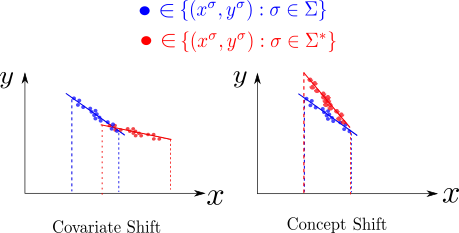
\includegraphics[width=4in]
{dataset-shift/dataset-shift.png}
\caption{For Linear Regression, 2 types
of dataset shift: covariate shift and concept shift.}
\label{fig-dataset-shift}
\end{figure}

\section{Covariate Shift}

We say there is a {\bf  covariate shift}
if (see Fig.\ref{fig-dataset-shift})

\beq
P( y|x)= P^*(y|x)
\text{ but } P(x)\neq P^*(x)
\eeq
This can be represented in terms of bnets as
follows\footnote{See
See Chapter \ref{ch-sb-removal}.}

\beq
\begin{array}{ccc}
\underbrace{\xymatrix{
\rvs=0 \ar[d]
\\
{\rvx}\ar[r]&\rvy
}}_
{\xymatrix{\\=}\xymatrix{
\rvs=0
\\
{\rvx}\ar[u]\ar[r]&\rvy
}}
&
\xymatrix{\\\neq}
&
\xymatrix{
\rvs=1\ar[d]
\\
{\rvx}\ar[r]&\rvy
}
\end{array}
\eeq


\section{Concept Shift}
We say there is a {\bf  concept shift}
if (see Fig.\ref{fig-dataset-shift})

\beq
P( y|x)\neq P^*(y|x)
\text{ but } P(x)= P^*(x)
\eeq
This can be represented in terms of bnets as
follows\footnote{See
See Chapter \ref{ch-sb-removal}.}

\beq
\begin{array}{ccc}
\underbrace{\xymatrix{
\rvs=0 \ar[rd]
\\
{\rvx}\ar[r]&\rvy
}}_
{\xymatrix{\\=}\xymatrix{
\rvs=0
\\
{\rvx}\ar[u]\ar[r]&\rvy\ar[lu]
}}
&
\xymatrix{\\\neq}
&
\xymatrix{
\rvs=1\ar[dr]
\\
{\rvx}\ar[r]&\rvy
}
\end{array}
\eeq

\section{Batch Normalization}
Batch Normalization (BN) is a technique
that is used to diminish dataset shift in Neural Nets.

Let
$h^{\lam, \s}_i$ be the output,
for individual $\s\in\Sigma$,  of the $i$th node
of layer $\lam$ of a Neural Net (NN).
Using the notation of Chapter \ref{ch-nn},

\beq
h^{\lam, \s}_i=
\cala_i^\lam(z^{\lam,\s}_i)
\eeq
where

\beq
z^{\lam,\s}_i=
\sum_j w^{\lam}_{i|j}
h^{\lam-1,\s}_j + b^{\lam}_i
\label{eq-linear-nn}
\eeq
Activation functions  $\cala^\lam_i:\RR\rarrow \RR$
for NNs
are discussed in Section \ref{sec-activation-fun}.
Suppose the population $\Sigma$ is partitioned
into disjoint batches $\Sigma^{(b)}$ for $b=1,2,\dots, B$.
Let the set of points $\{z^{\lam, \s}_i:\s\in\Sigma^{(b)}\}$
have mean $\mu^{\lam(b)}_i$
and standard deviation $\s^{\lam(b)}_i$.
For any $z^{\lam, \s}_i$ with $\s\in\Sigma$, define
the BN activation function
$\cala^\lam_{i, BN}(\cdot)$ by
\beq
\cala^\lam_{i, BN}(z^{\lam, \s}_i)=
\gamma^\lam_i
\left[
\frac{z^{\lam, \s}_i-\mu^{\lam(b)}_i}{\s^{\lam(b)}_i}
\right]+\beta^\lam_i
\quad
\text{ if }\s\in \Sigma^{(b)}
\;,
\eeq
where the real valued parameters $\gamma^\lam_i$ and $\beta^\lam_i$
are learned during the optimization process.
If node $\rvh^\lam_i$ of the NN has activation function
 $\cala^\lam_i:\RR\rarrow \RR$,
defined a new activation function $\cala^\lam_{i, new}:\RR\rarrow \RR$ by
the composition of functions
\beq
\cala^\lam_{i, new}
 =\cala^\lam_i\circ\cala^\lam_{i, BN}
\eeq
Hence, the BN activation
function
is applied after the linear transformation
Eq.(\ref{eq-linear-nn}), but before the nonlinear
transformation $\cala^\lam_i$.

Intuition on why BN diminishes dataset shift:
We discussed in Section \ref{sec-activation-fun}
how nonlinear activation functions
have a range that is smaller than their domain. Presumably, BN
helps to make the range
of the activation functions even more concentrated.

\chapter{Decision Trees}\label{ch-dtree}
This chapter is based 
mainly on Ref.\cite{stu-nor-book}.

\begin{figure}[h!]
\centering
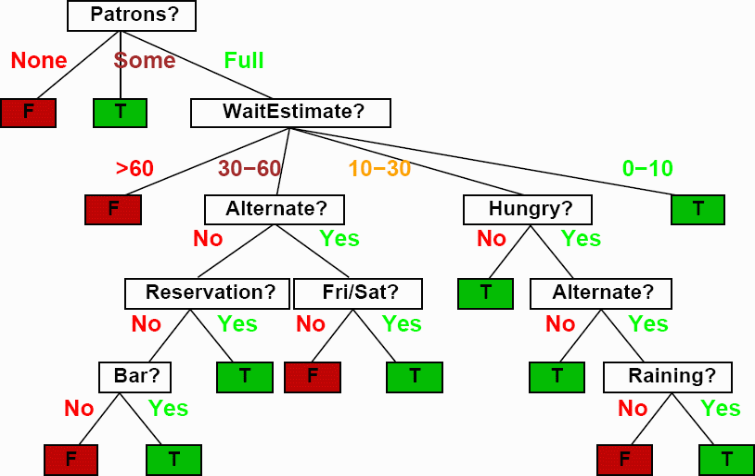
\includegraphics[width=4in]
{dtree/dtree-waiting.png}
\caption{Example of dtree taken from Ref.\cite{stu-nor-book}} 
\label{fig-dtree-waiting}
\end{figure}


\begin{figure}[h!]
\centering
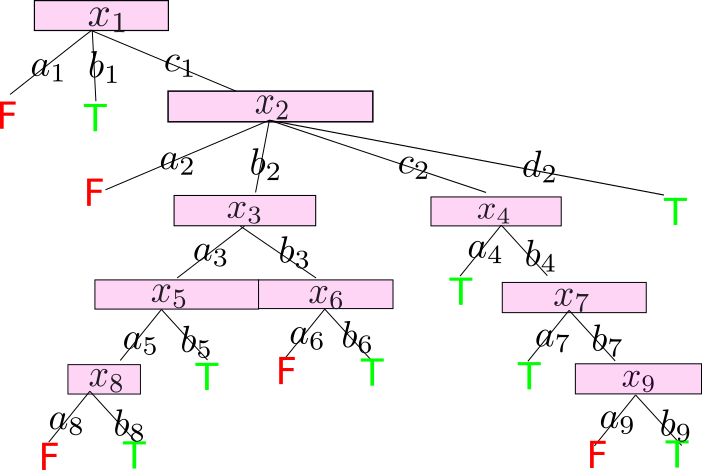
\includegraphics[width=3.2in]
{dtree/dtree-waiting-labels.png}
\caption{Fig.\ref{fig-dtree-waiting} with
abridged labels.} 
\label{fig-dtree-waiting-labels}
\end{figure}

\begin{figure}[h!]
\centering
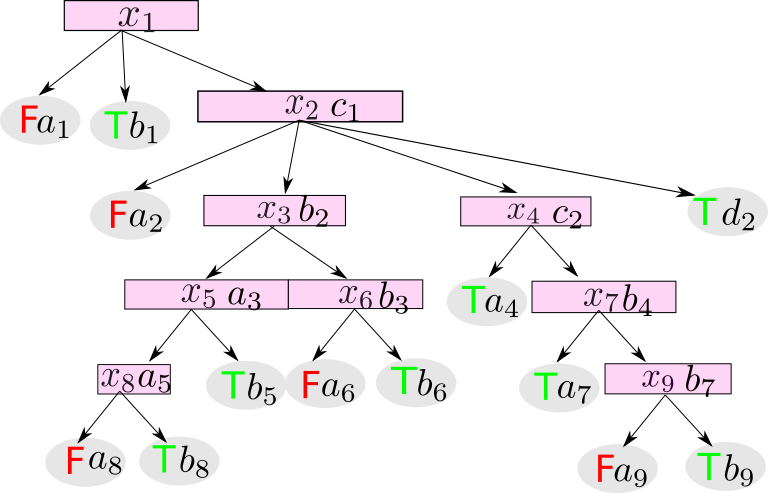
\includegraphics[width=3.2in]
{dtree/dtree-waiting-dags.png}
\caption{Fig.\ref{fig-dtree-waiting-labels}
converted to a bnet.} 
\label{fig-dtree-waiting-dags}
\end{figure}

Fig.\ref{fig-dtree-waiting}
shows a typical decision tree (dtree).
This example was taken
from Ref.\cite{stu-nor-book},
where it is analyzed
in detail.
As you can see,
a dtree contains two main types
of nodes: the non-leaf nodes,
and the leaf nodes.
The {\bf non-leaf nodes} pose
{\bf questions}. In general,
the {\bf answers}\footnote
{The {\bf question-answer pairs}
in dtrees are
also called
{\bf attribute-value pairs}.
Attributes are also
called {\bf features}.}
 to those
questions can
be multiple choices with
two or more choices.
For each of those choices,
a tree branch labeled by the choice
 comes down from the 
question node.
The {\bf leaf nodes} represent
endpoints, goals, final
conclusions, etc.
Dtrees can be viewed
as classifiers. They
take in a large amount 
of information about a population 
and compress that information
to just a few classes.
If $S_\rvc$ is the 
set of distinct leaf node labels,
then we call each
$c\in S_\rvc$
a  {\bf class of the classifier}.
In the case of
Fig.\ref{fig-dtree-waiting},
$S_\rvc=\{False, True\}$.

Dtrees can be used 
with
probabilities attached to each node, or without
probabilities
(as a
plain undirected graph(UG)).
This is analogous to bnets,
which can be used with
probabilities attached to each node
 (as DAGs with
TPMs specified for each node) or without
probabilities (as plain
DAGs).
Dtrees differ 
from bnets in that
their tree branches 
are labelled, whereas bnet arrows
 aren't labelled.
Also,
whereas the nodes of
a bnet carry a matrix of 
probabilities (the TPM),
the nodes of a dtree carry
just a column vector
of probabilities
which represents
a single 
probability distribution.
Henceforth,
we will refer to
the column vector
of probabilities
carried by each node of a dtree
as its {\bf Transition
Probability Vector (TPV)}.
Without the TPVs,
a dtree can be used 
as a deterministic classifier,
to classify inputs.
With the TPVs,
it can be used as a 
probabilistic sampler (to generate
random samples.)

\section{Transforming a dtree into a bnet}
A trivial 
observation
that is seldom made
in the dtree pedagogical literature
is that every dtree 
maps into a special bnet, 
let's call it
its ``image" bnet,
in a very natural way.
We use the dtree
of Fig.\ref{fig-dtree-waiting}
as an example to show 
how to do this. As 
a first 
step,
we go from
Fig.\ref{fig-dtree-waiting}
to
Fig.\ref{fig-dtree-waiting-labels}
by
replacing
all the labels of the
nodes and of the branches of
the dtree 
by abridged symbols. 
Next, we go 
from Fig.\ref{fig-dtree-waiting-labels}
to Fig.\ref{fig-dtree-waiting-dags},
by replacing all tree branches 
by arrows pointing down,
 and by
moving the tree branch labels 
down so that they
become a suffix to the question 
that the tree branch leads to.
At this point,
we have created
Fig.\ref{fig-dtree-waiting-dags},
which constitutes
the DAG of the image bnet.
It remains for us to define
a TPM for each node
of this DAG.

\begin{table}[]
\centering
\begin{tabular}{|l|l|l|l|}
\hline
$P(x|a)$ & \cellcolor[HTML]{ECF4FF}$a=a_0$ & \cellcolor[HTML]{ECF4FF}$a\in S^-_\rva-\{a_0\}$ & \cellcolor[HTML]{ECF4FF}$null$ \\ \hline
\cellcolor[HTML]{ECF4FF}0 & $p_0$ & 0 & 0 \\ \hline
\cellcolor[HTML]{ECF4FF}1 & $p_1$ & 0 & 0 \\ \hline
\cellcolor[HTML]{ECF4FF}$\vdots$ & $\vdots$ & 0 & 0 \\ \hline
\cellcolor[HTML]{ECF4FF}$N^-_\rvx-1$ & $p_{N_\rvx-1}$ & 0 & 0 \\ \hline
\cellcolor[HTML]{ECF4FF}$null$ & 0 & 1 & 1 \\ \hline
\end{tabular}
\caption{TPM of a node of a dtree image bnet.}
\label{tab-dtree-tpm}
\end{table}


Table \ref{tab-dtree-tpm}
gives the 
TPM $P(x|a)$
for a node $\rvx$
with single parent $\rva$
of a dtree image bnet. 
Say node $\rvx$ has 
a set $S^-_\rvx$
of possible tree branches
coming out of it. 
Let $N^-_\rvx = |S^-_\rvx|$.
Let $S_\rvx=S^-_\rvx\cup \{null\}$
and $N_\rvx=|S_\rvx|=N^-_\rvx+1$.
Define $S^-_\rva$, $N^-_\rva$,
$S_\rva$
and $N_\rva$
analogously for node $\rva$.
In Table \ref{tab-dtree-tpm},
$S^-_\rvx=\{0,1, \ldots, N^-_\rvx-1\}$
and 
$a_0$ is the value
of node $\rva$ which 
labels the tree branch
connecting nodes $\rva$ and $\rvx$.
$\vec{p}=(p_0, p_1, \ldots, p_{N_\rvx-1})$
is a probability
distribution 
associated with node $\rvx$,
its TPV.
TPVs
can be learned from
a dataset
following
the dtree Structure Learning (SL)
algorithm
discussed in Section \ref{sec-dtree-sl}.

Table \ref{tab-dtree-tpm}
also applies when node $\rvx$
is a leaf node,
except that for leaf nodes,
$\vec{p}$ is one hot (i.e., 
all components are zero 
except for one 
component which is 1).
Also, all 
leaf nodes
$\rvx$ have the same $S^-_\rvx$,
namely $S_\rvc$.


Adding a null state
to the set of states (SOS) of each node 
of the image bnet
is necessary
because, once $null$
is added 
to the SOS of any node,
it must be added to the SOS
 of all descendant
nodes.
$null$ must be added to the 
SOS of the children of
the root node
to
take care of the situations
when those first children
don't receive the state 
they were expecting from their
parent, i.e., the root node.


When drawing dtrees,
some people put
info 
like explanations 
and probabilities on the
branches
of  the dtree.
That
info can all
be preserved
in the TPM
and  the
node names and
 node state names
of the image bnet nodes.
One can also place info
inside tool tips attached to
the node name and node state names.
Often,
the pedagogical literature
states that 
dtrees are more explicit and  
carry
more info than their
image bnets,
but if one 
follows the above
prescriptions,
both can carry
the same info.



A naive Bayes (NB) bnet 
(see Chapter \ref{ch-naive})
consists of a single ``class node"
with states $S_\rvc$ that fans
out with arrows 
pointing to the
``feature nodes".
If each leaf node
of a NB bnet
fans out into 
a set of new leaf
nodes, and those new
leaf nodes
also
fan out
and so on,
we get a 
generalized NB bnet.
Let's call
this type of tree bnet an $NB^*$ bnet.
An $NB^*$ bnet
has the same graph structure
as the image bnet of a dtree,
but it's more general,
because its 
TPMs are more general. 
Each 
TPM of a $NB^*$ bnet
 can have several non-trivial
columns instead of just one
TPV= $\vec{p}$.


\section{Structure Learning for  Dtrees}\label{sec-dtree-sl}



Let

$J_0=\{0,1, \ldots, nj-1\}$

$\Sigma=\{0,1,2, \ldots,nsam-1\}$

$DS=\{(\s, x^\s, c^\s): \s\in \Sigma\}$ be a dataset

$\s\in \Sigma$ be an individual (a sample)
from a population, 

$x^\s\in S_\rvx$ be the {\bf
feature (attributes, questions) vector}.
$S_\rvx= S_{\rvx_0}\times S_{\rvx_1}
\times\ldots\times S_{\rvx_{nj-1}}$,
$x=(x_0, x_1, \ldots, x_{nj-1})\in S_\rvx$, 
$x_j\in S_{\rvx_j}$


$c^\s\in S_\rvc$ be a {\bf classification class}

We will
assume $S_\rvx$ and $S_\rvc$ are finite sets.

Building a {\bf classifier $Y$} 
(curve fit) for a dtree means
finding a deterministic
function $Y:S_\rvx\rarrow S_\rvc$ 
such that 
$c^\s \approx Y(x^\s)$
for all $\s\in \Sigma$.
If we divide
the population
$\Sigma$ 
into two large 
disjoint
sets, a {\bf training set} $\Sigma_{train}$
and a {\bf validation set} $\Sigma_{vali}$,
and if $c^\s \approx Y(x^\s)$ very closely
for $\s\in \Sigma_{train}$
but fits poorly
for $\s\in \Sigma_{vali}$,
then we say the classifier  $Y$
suffers from {\bf overfitting}.
We can learn the structure
and TPVs of a dtree from a dataset $DS$,
by using the
dtree {\bf Structure Learning (SL)}
algorithm that we will 
discuss in detail later. However,
that algorithm
is prone to produce
a classifier $Y$ that overfits.
Two techniques 
commonly used to 
reduce the effects of overfitting
are {\bf pruning}  and 
{\bf Random Forest (RF)}
(see Chapter \ref{ch-rforest}).
Pruning just means somehow
removing nodes that are
too specific. 
An RF is an ensemble of dtrees 
that one averages over.
In this chapter, we will only deal
with a single dtree,
not an ensemble of them. 

Dtree SL was invented in 1984-1986 so it
is fairly old.
Many in the AI
community 
consider dtrees old fashioned
compared to neural nets.
But dtrees 
are {\bf interpretable} whereas neural nets aren't.\footnote{
To be precise, only
plain dtrees without boosting or
 bagging
are interpretable.
Dtrees used within boosting
(see Chapter \ref{ch-adaboost} on AdaBoost
and
Chapter \ref{ch-xgboost} on XGBoost)
or bagging
(see Chapter \ref{ch-rforest} on Random Forest)
gain much
accuracy but lose
{\bf interpretability}.}
Bnets are interpretable too.


Below,
we give the standard
algorithm for SL
of a dtree, in the form
of pseudo-code.
But first,
we define
two quantities,
Information Gain and
Gini,
that are 
used in that 
pseudo-code.


\subsection{Information Gain, Gini}
This section uses various Shannon Information Theory
entropies. Our 
notation for those
entropies
is described in Chapter \nameref{ch-conventions}.


Call a {\bf separation ability measure} (SAM)
a measure used 
to decide, when 
constructing a dtree from a dataset,
in what order 
to ask the questions
about the feature vector $x$.
The question order is decided
by searching 
over all so far unused questions
for the question with 
the largest SAM.\footnote{SAM
is also called, somewhat
confusingly, the splitting
criterion and Gain.}



\begin{figure}[h!]
$$
\xymatrix{
&
\\
\rvx_j\ar[r]_{\rvx_j=x_j}
\ar[ru]^{\rvx_j=x_j'}&
\\
\{N_j(c,x_j)\}_{c\in S_\rvc, x_j\in S_{\rvx_j}}
\\
\sum_{c\in S_\rvc}N_j(c,x_j)=N_j(x_j)
\\
\sum_{x_j\in S_{\rvx_j}}N_j(c,x_j)=N_j(c)
&
\sum_{c\in S_\rvc}N_j(c)=
\sum_{x_j\in S_{\rvx_j}}N_j(x_j)=N_j
}
$$
\caption{
Some population numbers associated
with the nodes of a dtree. $N_j(c, x_j)$ is the number
of individuals $\s$
in the population that reaches node $j$,
belonging to class $c$ and having $\rvx_j=x_j$.} 
\label{fig-dtree-notation}
\end{figure}
\begin{figure}[h!]
$$
\xymatrix{
\rvj
\ar[r]\ar@/^1pc/[rr]
&
\rvx_j \ar[r]
&
\rvc
}$$
\caption{Bnet derived from population
numbers in Fig.\ref{fig-dtree-notation}}
\label{fig-class-bnet}
\end{figure}



Fig.\ref{fig-dtree-notation}
defines some population numbers
associated
with the nodes of a dtree.
From these population numbers, we can define
the bnet in Fig.\ref{fig-class-bnet}.
The TPMs, printed in blue,
for the (non-root) nodes of this bnet, are as follows

\beq\color{blue}
P(c|x_j,j)=
\frac{N_j(c,x_j)}
{N_j(x_j)}
\eeq

\beq\color{blue}
P(x_j|j)=
\frac{N_j(x_j)}
{N_j}
\eeq
where $j\in J_0$
$x_j\in S_{\rvx_j}$, and
$c\in S_\rvc$ is a class node.



One can define the following 
information theory quantities\footnote{
The average of $H(\rvc:b)$ over
$b$ is $H(\rvc:\rvb)=\sum_bP(b)
H(\rvc:b)$.
Likewise,
the average of
$H(\rvc|b)$ over $b$ is 
$H(\rvc|\rvb)=\sum_b P(b)H(\rvc|b)$.
$H(\rvc:\rvb)$ 
becomes $H(\rvc:b)$
and $H(\rvc|\rvb)$
becomes $H(\rvc|b)$
when there is no $b-$prior (i.e., 
$P(b)$ is a delta function).
}
associated with the bnet Fig.\ref{fig-class-bnet}.


\beqa
INFO\_fin_j&=& 
-\sum_c P(c|j)\ln P(c|j)
\\
&=&
H(\rvc|j)
\\
\eeqa




\begin{align}
INFO\_init_j
&=
\sum_{x_j\in S_{\rvx_j}} P(x_j|j)H(\rvc|x_j,j)
\\
&=
H(\rvc|\rvx_j , j)
\end{align}



\beqa
IG_j&=&
INFO\_fin_j- INFO\_init_j
\\
&=&
H(\rvc|j)-H(\rvc|\rvx_j , j)
\\
&=& H(\rvc:\rvx_j |j)
\label{eq-info-gain}
\eeqa
$IG_j$
is called the {\bf
information gain
for node $\rvx_j$}.
Maximizing this mutual information
produces 
a node $\rvx_j$ that has 
a large correlation
to a class $c$.
If the  
goal is to reach
a point 
where each leaf node is
closely correlated
to a different class,
then maximizing the
Information Gain
of each new node
is a greedy move
towards that goal.
Thus, Information Gain
is a good 
SAM
for dtree SL.

Note that if we approximate

\beqa
\ln  P(c|x_j)
&\approx&
\ln [1 + P(c|x_j)-1]
\\
&\approx&
P(c|x_j)-1
\eeqa
in $H(\rvc|x_j)$,
we get what is called 
the {\bf Gini (or Gini Index)
for node $\rvx_k$}:


\beqa
H(\rvc|x_j)
&=&
-\sum_c P(c|x_j)\ln P(c|x_j)
\\
&\approx&
1 -\sum_{c\in S_{\rvc}} P(c|x_j)^2
\eqdef
 Gini_{x_j}
\eeqa
$Gini_{x_j}$
is a fairly good
polynomial approximation
to $H(\rvc|x_j)$.
It is computationally
much less expensive than
$H(\rvc|x_j)$,
because it does not
require computing a log.

We say 
a probability 
distribution $P_\rvx$, is {\bf pure (i.e., deterministic)}
 if $P_\rvx(x)=\delta(x, x_0)$. $Gini_{x_j}$
 and $H(\rvc|x_j)$ are both always
non-negative.
They both vanish iff  
$P(c|x_j)$ is pure.
Thus, $Gini_{x_j}$ and  $H(\rvc|x_j)$ 
are both good measures of  {\bf class impurity}.

The {\bf average Gini of node $\rvx_j$} is defined as

\beq
AGini_j
=
\sum_{x_j\in S_{\rvx_j}}
P(x_j|j)
 Gini_{x_j}
\;.
\eeq
It measure 
the average impurity
of the children of node $\rvx_j$.



\begin{mdframed}[hidealllines=true,backgroundcolor=gray!10]
In practice, the
SL algorithm
is done recursively.
Each 
recursion
step 
decides
which feature $x_j$
will be the root 
node of the current tree.
For all ``candidate" features
(i.e., all $\rvx_j$
that haven't been used yet 
as tree nodes), one
calculates
$IG_j$,
either
exactly
or approximately via Gini's,
using the following formula:

\beq
IG_j=
\underbrace{H(\rvc|j)}_{\approx Gini_j}
-
\sum_{x_j\in S_{\rvx_j}}
P(x_j|j)
\underbrace{H(\rvc|x_j)}_
{\approx Gini_{x_j}}
\eeq
One then chooses $j=\argmax_j IG_j$. This
maximizes the $\rvc-\rvx_j $ correlation.

Alternatively,
some software programs use
the average Gini
$AGini_j$
as their SAM. They
choose
as root node
 $j=\argmin_j AGini_j$.
This minimizes the average impurity
of the children of node $j$.
Since $IG_j$
differs from $AGini_j$ by $H(\rvc|j)$,
maximizing $IG_j$
and
minimizing $AGini_j$
might lead  to different results.
\end{mdframed}
\hrule\noindent{\bf Example of calculation of $AGini_j$ 
and $IG_j$}

Suppose we deduce from a dataset
the numbers in the yellow cells
in Table \ref{tab-temp-gini}.
These numbers are repeated in  Fig.\ref{fig-stump-3cildren}.
Then we can calculate the white cells as follows: 

% Please add the following required packages to your document preamble:
% \usepackage[table,xcdraw]{xcolor}
% If you use beamer only pass "xcolor=table" option, i.e. \documentclass[xcolor=table]{beamer}
\begin{table}[h!]
\centering
\begin{tabular}{|l|l|l|l|}
\hline
$j=temp?$ & \cellcolor[HTML]{CBCEFB}$x_j=hot$ & \cellcolor[HTML]{CBCEFB}$x_j=med$ & \cellcolor[HTML]{CBCEFB}$x_j=cold$ \\ \hline
\rowcolor[HTML]{FFFFC7} 
\cellcolor[HTML]{9AFF99}$c=play$ & 3 & 3 & 3 \\ \hline
\rowcolor[HTML]{FFFFC7} 
\cellcolor[HTML]{FFCCC9}$c=stay$ & 1 & 2 & 2 \\ \hline
$Gini$ & 0.375 & 0.48 & 0.48 \\ \hline
\multicolumn{4}{|l|}{$AGini=0.45$} \\ \hline
$H(\rvc|x_j)$ & $\approx 0.375$ & $\approx 0.48$ & $\approx 0.48$ \\ \hline
\multicolumn{4}{|l|}{$IG\approx 0$} \\ \hline
\end{tabular}
\caption{Evaluating AGini and IG for node $temp$.}
\label{tab-temp-gini}
\end{table}



\begin{figure}[h!]
\centering
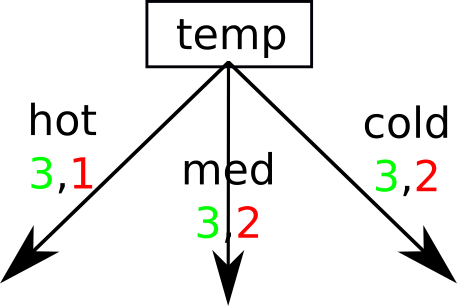
\includegraphics[width=1.5in]
{dtree/stump-3children.png}
\caption{Tree stump
corresponding to Table \ref{tab-temp-gini}.}
\label{fig-stump-3cildren}
\end{figure}



\begin{itemize}
\item Gini(hot)$=1-(3/4)-(1/4)=0.375$
\item Gini(med)$=1-(3/5)^2-(2/5)^2=0.48$
\item Gini(cold)$=1-(3/5)^2-(2/5)^2=0.48$
\item AGini $ = (4/14)(0.375)+
(5/14)(0.48) + (5/14)(0.48) = 0.45 $
\item IG $\approx [1 -(6/9)^2-(3/9)^2]-AGini= 
0.44-0.45\approx 0$
\end{itemize}

This gives
the AGini and IG for just one 
candidate root node.
We would have
to calculate
AGini (or IG) for all
possible candidates
and choose the candidate
with the lowest AGini (or highest IG).


\section{Information Gain Ratio}

The Information Gain Ratio (IGR) is an alternative SAM.

\beqa
IGR_j
&=&
\frac{IG_j}{H(\rvx_j |j)}
\\
&=&
\frac{H(\rvc:\rvx_j |j)}{H(\rvx_j |j)}
\\
&=&
\frac{H(\rvx_j |j)-H(\rvx_j |\rvc, j)}
{H(\rvx_j |j)}
\\
&=&
1 - \frac{H(\rvx_j |\rvc, j)}{H(\rvx_j |j)}
\eeqa

$0\leq IGR_j\leq 1$

$IGR_j=0$ iff $H(\rvx_j |\rvc, j)=H(\rvx_j |j)$.




\subsection{Pseudo-code}

Below,
we give the standard
algorithm for SL
of a dtree, in the form
of pseudo-code.
The strategy
employed by
the algo
is to assume an incoming
population into the current root node,
then
determine the feature $x_j$
 that best separates that 
incoming
population. The feature
$x_j$ is chosen so as to maximize
$IG_j$
(or minimize $AGini_j$). This
process is repeated by nominating
the end of each new branch to be
the current root node.
Features can appear as a node 
more than once, so the order in 
which nodes are split does not matter.
In essence, what we are doing is
performing a top-down, greedy search
through the space of possible dtrees.

The pseudo-code below describes the following 
historically important
software programs:
\begin{itemize}
\item CART (Classification and Regression Trees),
invented by Breiman et al in 1984. Uses $AGini_j$ as SAM.
\item
ID3 (Iterative Dichotomiser 3)
invented by Quinlan in 1986. Uses $IG_j$ as SAM.
C4.5/C5.0 are successors to ID3.
\end{itemize}

Thus, CART and ID were 
invented independently around the same time.
The main difference between them is the SAM
being used.


The pseudo-code below
uses the majority function
defined in Chapter \nameref{ch-conventions}.


\begin{algorithm}
	\DontPrintSemicolon
    \SetKwInOut{KwIn}{Input}
    \SetKwInOut{KwOut}{Output}
    \caption{Pseudo-code for learning a dtree from a dataset}
	\KwIn{dataset $DS=\{(\s, x^\s, c^\s): \s\in \Sigma\}$,\\ 
	set of currently available node indices 
	$J$, where $J\subset J_0$}
	\KwOut{tree $T$,\\
		population numbers $\{(r,c,x_r,N_r(c, x_r)):
			r\in J_0, c\in S_\rvc,
			x_r\in S_{\rvx_r}\}$ stored globally}
	\;
	From $DS$, calculate $J_0$, $S_\rvc$, $S_{\rvx_i}$ for each $i$ \\
	$c^\s$ is called the target feature/attribute.\\
	$J\larrow J_0$\;
	\SetKwFunction{FMain}{learn\_dtree}
	\SetKwProg{Fn}{Function}{:}{}
	\Fn{\FMain{$DS, J$}}{
		$\Sigma\larrow$ set of all $\s$ in $DS$\; 
		\If{$\{c^\s:\s\in\Sigma\}=\{c\}$ }{
			$T\larrow$ one node tree with leaf node label= $c$\;
		}
		\ElseIf{$J=\emptyset$}{
			$T\larrow$ one node tree with leaf node label=
			{\tt majority}$([ c^\s:\s\in\Sigma])$\;
		}
		\Else{
			$r\larrow \argmax_{j\in J}IG_j(DS)$
			\tcp{or replace $\argmax_{j\in J}IG_j$ 
			by $\argmin_{j\in J}AGini_j$}\;
			from $DS$, calculate $\{(r,c,x_r, N_r(c,x_r)):
			c\in S_\rvc,x_r\in S_{\rvx_r} \}$ and 
			store it globally\;
		\For{$v\in S_{\rvx_r}$}{
			\tcc{Notice that $J$ is the same every time repeat this loop,
			so order in which $v\in S_{\rvx_r}$ are called does not matter.
			Furthermore, this means that multiple tree nodes may be labeled by same feature.}
			On current tree $T$, add  a branch below $\rvx_r$ with label 
			``$\rvx_r = v$"\;
			$DS|_{\rvx_r=v}\larrow$ subset of $DS$ with $\rvx_r = v$\;
			\If{$DS|_{\rvx_r=v}=\emptyset$}{
				below the new branch add a \\leaf node labeled = 
				{\tt majority}$([c^\s:\s\in\Sigma])$\;
			}
			\Else{
				below the new branch add \\
				subtree =$ {\tt learn\_dtree}
				(DS|_{\rvx_r=v}, J-\{r\})$\;
			}			
    	}
		}
		\KwRet $T$\;
	}
\end{algorithm}


\chapter{Decisions Based on Rungs 2 and 3: COMING SOON}
\label{ch-dec-2-3}


\chapter{Difference-in-Differences}
\label{ch-did}

This chapter is based on
Ref.\cite{book-mixtape}.


The Difference-in-Differences (DID)
method was first used by John Snow
in an 1854 report that
argued that 
cholera in London
was being transmitted 
by sewage polluted water
rather than, as others
at the time believed, by air (in fetid vapors
called miasmas).
In general, one can
apply DID to discover 
causal effects in historical data.
By {\bf historical data} (aka a {\bf natural
experiment}. See Ref.\cite{wiki-nat-exp})
we mean data that is collected long
after the treatment (rather than during it)
 and is thus
not  subject to 
active intervention
by the experimenter. 

This chapter assumes that the
reader has read Chapter \ref{ch-pot-out}
on Potential Outcomes (PO).
The DID method
applies the basic single-time
PO theory described in Chapter \ref{ch-pot-out},
to 2
well separated times
in which
different conditions prevail.



\section{John Snow, DID  
and a cholera
transmission pathway}


\begin{figure}[h!]
\centering
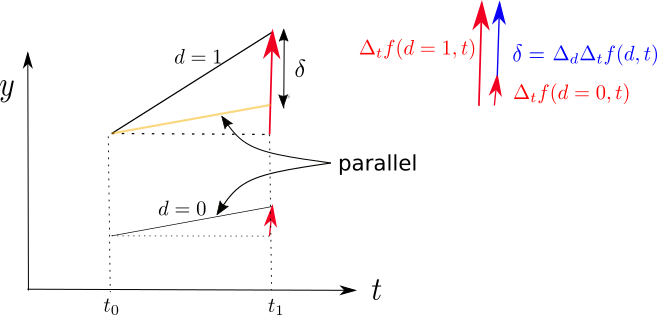
\includegraphics[width=5in]
{did/dif-dif.png}
\caption{Pictorial representation of
 Difference-in-differences (DID) as a difference
of two differences (i.e., 
a difference of two slopes).} 
\label{fig-dif-dif}
\end{figure}

Let

$d\in \bool$

$t\in \{t_0, t_1\}$, $t_0< t_1$

$y=f(d,t)\in \RR$.

Define

\beq
\Delta_t f(d,t)= f(d, t_1)-f(d, t_0)
\;,
\eeq

\beq
\Delta_d f(d, t)= f(1, t)-f(0, t)
\;,
\eeq

\beq
DID=\delta=\Delta_d\Delta_t f(d,t)
\;.
\eeq
DID is illustrated in
 Fig.\ref{fig-dif-dif}. 


A {\bf time series} 
is  any function of time
for which the domain is a discrete set of times.




\begin{figure}[h!]
\centering
\includegraphics[width=4in]{did/did-3-prod}
\caption{$DID=\delta$ expressed as 
difference of slopes or 
difference of vectors.} 
\label{fig-did-3-prod}
\end{figure}

Note that,
as shown Fig.\ref{fig-did-3-prod},
$DID=\delta$ can also be expressed
as a difference of 2 slopes
times $\Delta t = t_1-t_0$.
Let
$\hat{y}$ be a unit 
in the $y$ direction.
$\delta$ can also be expressed
as the dot product of a difference of 2 vectors
dotted with $\hat{y}$.


\begin{table}[h!]
\centering
{\renewcommand{\arraystretch}{1.4}
\begin{tabular}{|c|c|c|}
\hline 
\rowcolor[HTML]{ECF4FF} 
 & $t=t_0 $ (1849) & $t=t_1$ (1854) \\ 
\hline
$d=1 $ (town 1)\cellcolor[HTML]{ECF4FF}
&85 deaths, polluted DW&19 deaths, unpolluted DW\\
\hline 
$d=0 $ (town 0)\cellcolor[HTML]{ECF4FF} 
&135 deaths, polluted DW& 147 deaths, polluted DW\\ 
\end{tabular}
}
\caption{A condensation of the data
collected by 
John Snow in 1854,
to test the hypothesis
that cholera in London was being spread by
polluted drinking water (DW).}
\label{tab-john-snow}
\end{table}

A condensation of the
data collected by John Snow in 1854
is given in Table \ref{tab-john-snow}.
From that data, we find that

\beq
\delta= \Delta_d\Delta_t f(d,t)=(19-85)-(147-135)=
-66-12=-78
\eeq



\section{PO analysis}
In this section,
we show how
to analyze the
DID method
using the formalism of PO theory.

We will speak of a treatment 
outcome
$\rvy^\s_{t, g^\s}
(c^\s, x^\s)$
for individual $\s$
that depends, not 
just on the treatment dose 
$c^\s\in \bool$
and the confounder state $x^\s$,
but also
on a group parameter (i.e., which population
or town)
$g^\s\in \bool$
and on a time parameter $t\in\{t_0, t_1\}$ 
(note $t$ is independent of $\s$).
Actually,
we will assume $g^\s=c^\s$,
so we will just speak of
$\rvy^\s_t(c^\s, x^\s)$
with no explicit $g^\s$
dependence. As usual for PO theory,
we will consider
expected values of $y^\s_t$:


\beq
E_{\s|\td, x}[y^\s_t(c)]=
 E_{y_t|\td, x}[\rvy_t(c)]=
\caly_{c|\td, x}(t)
\eeq

To calculate these
expected values, we need a ``model"
with probability 
distributions.
In this case,
the needed model and probability
distributions are
provided by the
bnets depicted in Fig.\ref{fig-did-G_t-im}.
The TPMs,
printed in blue,
for the 
 bnet
$G_{t, im}$
in Fig.\ref{fig-did-G_t-im},
are as follows.
Note
that the
TPMs for the bnet $G_{t, im}$
are defined in 
terms
of the TPMs for the bnet $G_t$.


\begin{figure}[h!]
$$
\begin{array}{ccccc}
\xymatrix{
&\rvx^\s\ar[dl]\ar[dr]
\\
\rvd^\s\ar[rr]&&\rvy^\s_t
}
&&
\xymatrix{
&\rvx^\s\ar[dl]\ar[dr]
\\
\rvd^\s=d^\s&\rvtd^\s=\td^\s\ar[r]&\rvy^\s_t
}
\\
\\
G_t&&G_{t, im}
\end{array}
$$
\caption{$t\in \{t_0, t_1\}$.
Bnet 
$G_{t, im}= \kappa_{\rvd^\s\rarrow\rvy^\s_t}
(\td^\s)G_t$
is obtained by applying 
the imagine operator to arrow 
$\rvd^\s\rarrow\rvy^\s_t$
of bnet $G_t$.}
\label{fig-did-G_t-im}
\end{figure}

\beq\color{blue}
P(x^\s)=P_\rvx(x^\s)
\eeq

\beq\color{blue}
P(d^\s|x^\s)= 
P_{\rvd|\rvx}(d^\s|x^\s)
\eeq
 
\beq\color{blue}
P(y^\s_t|\td^\s, x^\s)=
P_{\rvy_t|\rvd, \rvx}(y^\s_t|\td^\s, x^\s)
\eeq

\beq\color{blue}
P((\td^\s)')=\delta(
(\td^\s)', \td^\s)
\eeq

\begin{figure}[h!]
\centering
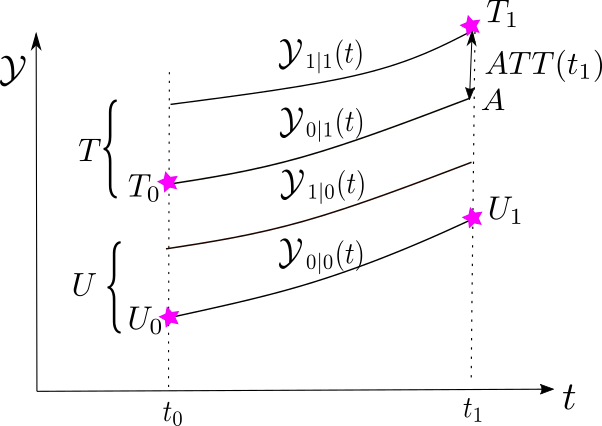
\includegraphics[width=3in]
{did/dif-dif-bc.png}
\caption{
Four different time-dependent
expected 
values $\caly_{c|\td}(t)$ of $y^\s_t$
for bnet $G_{t, im}$
The 4 magenta  stars
represents the 4 DID measurements.
} 
\label{fig-dif-dif-bc}
\end{figure}

Henceforth, 
for simplicity, we will
omit the confounder state $x$
from the indices of $\caly$; i.e., we will write
$\caly_{c|\td}(t)$
instead of $\caly_{c|\td, x}(t)$.
The fact that we will
not explicitly
mention $x$ does not
mean that it doesn't exist
or that it doesn't affect our analysis.
John Snow
does not seem to have considered any confounders
in his cholera study,
or else he tried to collect 
data restricted to a single stratum $x$.
If there are confounders,
they cannot be neglected.
As discussed in Chapter \ref{ch-pot-out}
under the subject of strata-matching in PO,
one must condition $\caly$
on a single $x$ stratum
and, later on,  one must average
over all the possible $x$ strata.



We define the function $c(t)$ for $t=t_0, t_1$ by

\beq
c(t)
=
\left\{
\begin{array}{ll}
0&\text{if $t=t_0$}
\\
\td&\text{if $t=t_1$}
\end{array}
\right.
\eeq
Now we claim that the DID 
$\delta$ calculated in the 
previous section for
John Snow's data,
can be expressed in PO formalism as follows:

\beq
\delta=
\Delta_\td\Delta_t
\caly_{c(t)|\td}(t)
\;.
\eeq
Fig.\ref{fig-dif-dif-bc}
depicts the
four functions
$\caly_{c|\td}(t)$
for $t$ in the interval  $[t_0, t_1]$
and for $c,\td\in \bool$.
The $\caly$ coordinates
of the four magenta stars in 
Fig.\ref{fig-dif-dif-bc} can 
be calculated using bnet $G_t$.

Define
the {\bf parallel trends} (PT)
by 

\beq
PT=\Delta_\td\Delta_t\caly_{0|\td}(t)
\;.
\eeq
We will say the 
{\bf parallel trends assumption (PTA)}
holds if $PT=0$.

Next we prove that
the DID $\delta$ equals
the sum of an ATT\footnote{ATT stands for 
the average treatment effect
of the treated. ATT is defined 
in Chapter \ref{ch-pot-out}}
and PT.

\begin{align}
\delta&=
\Delta_\td\Delta_t  
\caly_{c(t)|\td}(t)
\\
&=
\left[
\Delta_t \caly_{c(t)|1}(t)
-\Delta_t \caly_{c(t)|0}(t)
\right]
\\
&=
\caly_{1|1}(t_1)-\caly_{0|1}(t_0)
-\{
\caly_{0|0}(t_1)-\caly_{0|0}(t_0)
\}
\\
&=
\caly_{1|1}(t_1)-\caly_{0|1}(t_0)
-\{
\caly_{0|0}(t_1)-\caly_{0|0}(t_0)
\}
+\underbrace{
\{
\caly_{0|1}(t_1)-
\caly_{0|1}(t_1)
\}}_{\text{ zero }}
\\
&=
\underbrace{
\caly_{1|1}(t_1) - \caly_{0|1}(t_1)}
_{ATT(t_1)}
-\caly_{0|1}(t_0)
-\{
\caly_{0|0}(t_1)-\caly_{0|0}(t_0)
\}
 + \caly_{0|1}(t_1)
\\
&=
ATT(t_1)
-\Delta_t \caly_{0|0}(t)
+\Delta_t \caly_{0|1}(t)
\\
&=
ATT(t_1)
+
\underbrace{\Delta_\td\Delta_t\caly_{0|\td}(t)}_
{\text{ zero if PTA holds}}
\end{align}





\section{Linear Regression}
In this
section,
we show how to apply
linear regression (LR)
to the PO analysis of DID.


As before, let
$y^\s_t(c^\s)$ be the treatment outcome
for individual $\s$,
who receives
a treatment dose
$c^\s$
at times $t\in\{t_0, t_1\}$.
$y^\s_t(c^\s)$
can be fitted as follows.
Here $\eps^\s$
is the residual
for individual $\s$,
and $b_0, m_0, b_1, m_1\in \RR$
are the fit parameters.

\beq
y^\s_t = [b_0 + m_0 (t-t_0)](1-c^\s)
+  [b_1 + m_1 (t-t_0)]c^\s
+ \eps^\s
\;.
\label{eq-did-lr}
\eeq  
Note that Eq.(\ref{eq-did-lr})
 yields a straight line
in the $y^\s_t-t$ plane
for $c^\s=0$,
and another 
straight line for $c^\s=1$.
We are
using the
standard symbols
$b$ to denote
the y-intercept, and $m$ 
to denote the slope
of a straight line.

Taking the expected value
of Eq.(\ref{eq-did-lr}), we get

\beq
\caly_{c|\td}(t) = 
[b_0 + m_0 (t-t_0)](1-c)
+  [b_1 + m_1 (t-t_0)]c
\;.
\eeq  
If $\Delta  t = t_1-t_0$, then

\beq
\caly_{\td|\td}(t_1) = 
[b_0 + m_0 \Delta t](1-\td)
+  [b_1 + m_1 \Delta t]\td
\;,
\eeq
and

\beq
\caly_{0|\td}(t_0) = b_0
\;.
\eeq
 Thus,   

\beqa
\delta&=&\Delta_\td\Delta_t 
\caly_{c(t)|\td}(t)
\\
&=&
\Delta_\td[\caly_{\td|\td}(t_1)-\caly_{0|\td}(t_0)]
\\
&=&
(m_1-m_0)\Delta t
\;.
\eeqa



\begin{figure}[h!]
\centering
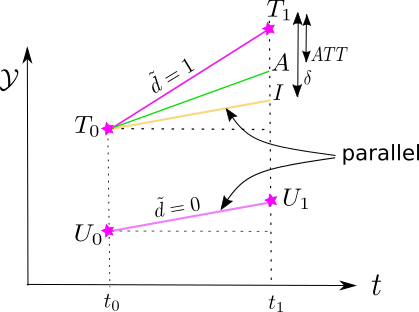
\includegraphics[width=3.5in]
{did/parallel-trends.png}
\caption{We use
Linear Regression
to fit a straight line
between points $U_0$
and $U_1$,
and between points
$T_0$ and $T_1$.
(U=untreated, T=treated, subscript refers
to times $t_0, t_1$).
$U_0, T_0, U_1, T_1$ are the measurement points.
Point
$I$ is an image of point $U_1$.
} 
\label{fig-parallel-trends}
\end{figure}

\begin{table}[h!]
\centering
{\renewcommand{\arraystretch}{1.2}
\begin{tabular}{|c|c|c|}
\hline 
\rowcolor[HTML]{ECF4FF} 
 & $t=t_0$ & $t=t_1$ \\ 
\hline
$\td=1$ \cellcolor[HTML]{ECF4FF}& 
$\caly(T_0)=\caly_{0|1}(t_0)$ & 
$\caly(T_1)=\caly_{1|1}(t_1)$ \\ 
\hline 
$\td=0$\cellcolor[HTML]{ECF4FF} & 
$\caly(U_0)=\caly_{0|0}(t_0)$ & 
$\caly(U_1)=\caly_{0|0}(t_1)$ \\ 
\hline 
\end{tabular}
}
\caption{
$\caly$ coordinates
of points
$U_0, T_0, U_1, T_1$
in Figs.\ref{fig-dif-dif-bc}
 and \ref{fig-parallel-trends}.
}
\label{tab-did-points}
\end{table}



Figs.\ref{fig-dif-dif-bc} and
\ref{fig-parallel-trends}
define
points $U_0, T_0, U_1, T_1, I, A$.
The $\caly$
coordinates of points 
$U_0, T_0, U_1, T_1$ are 
given by
Table \ref{tab-did-points}.
The $\caly$
coordinates of points $A,I$
are given by Eqs.\ref{eq-c-i-pts}.

\begin{subequations}
\label{eq-c-i-pts}
\beq
\caly(A)= \caly_{0|1}(t_1)
\eeq

\beq
\caly(I)=\caly(U_1) + 
[\caly(T_0)-\caly(U_0)]
\eeq
\end{subequations}

We can express $ATT$
and the $\delta$ for DID 
in terms of 
the $\caly$
of the points
$U_0, T_0, U_1, T_1, I, A$. Indeed,

\beqa
\delta&=&\caly(T_1)-\caly(I)
\\
&=&
\caly(T_1)-
\caly(U_1) -
[\caly(T_0)-\caly(U_0)]
\eeqa

\beq
ATT = \caly(T_1)-\caly(A)
\eeq
Hence, 

\beq
\delta=ATT\iff \caly(I)=\caly(A) \iff 
\text{PTA holds}
\eeq
\chapter{Digital Circuits}

\begin{figure}[h!]
\centering
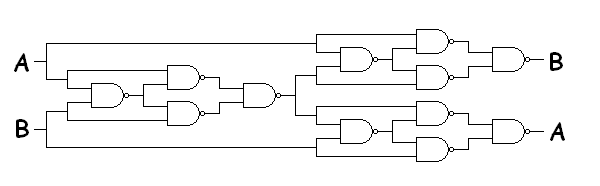
\includegraphics[width=6in]{d-ckt/d-ckt.png}
\caption{Typical digital circuit
of NAND gates.}
\label{fig-d-ckt}
\end{figure}

{\bf Digital (logic) gate:} node with
$na$ input ports and $nx$ output ports
which represents a function

\beq
f:\bool^{na}\rarrow \bool^{nx}
\;.
\label{eq-f-gate}
\eeq

Suppose

$a^{na}=(a_i)_{i=0, 1,\dots, na-1}$ 
where $a_i\in \bool$,

$x^{nx}=(x_i)_{i=0, 1,\dots, nx-1}$ 
where $x_i\in \bool$. 

$f$ maps $a^{na}$ into $x^{nx}$.

{\bf Digital circuit (dcircuit)} = circuit of digital gates.

\begin{figure}[h!]
\centering
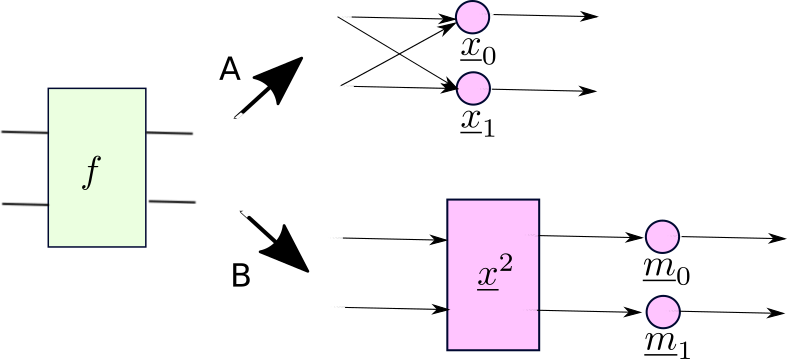
\includegraphics[width=3in]{d-ckt/d-ckt-2ops.png}
\caption{2 options
for mapping dcircuit node with
multiple output ports into bnet.}
\label{fig-d-ckt-2ops}
\end{figure}

\section{Mapping any
dcircuit to a bnet} 
\subsection{Option A of Fig.\ref{fig-d-ckt-2ops}}
\begin{enumerate}
\item
Replace every dcircuit  gate 
described by Eq.(\ref{eq-f-gate})
by
$nx$ bnet nodes $\rvx_i$
for $i=0, 1, \ldots, nx-1$
such that

\beq\color{blue}
P(x_i|a^{na})=\delta(x_i, f_i(a^{na}))
\eeq
\item
Replace
all connectors of the dcircuit
by arrows 
pointing in the direction
of the bit flow.

\end{enumerate}

\subsection{Option B of Fig.\ref{fig-d-ckt-2ops}}
\begin{enumerate}
\item
Replace every dcircuit  gate 
described by Eq.(\ref{eq-f-gate})
with
one bnet node called $\rvx^{nx}$
and, if $nx>0$, 
$nx$ ``marginalizer nodes" $\rvm_i$
for $i=0, 1, \ldots, nx-1$, such that

\beq\color{blue}
P(x^{nx}|a^{na})=
\delta(x^{nx}, f(a^{na}))
\;,
\eeq
and
\beq\color{blue}
P(m_i|x^{nx})=
\delta(m_i, x_i)
\;.
\eeq


\item
Replace
all connectors of the dcircuit
by arrows 
pointing in the direction
of the bit flow.



\end{enumerate}
\hrule 
Options A and B don't work
for digital circuits 
with feedback loops 
such as flip-flops.
Those could probably
be modeled with 
dynamical bnets.
\chapter{Do Calculus}\label{ch-do-calc}


The Do Calculus and associated ideas were
invented by
Judea Pearl and collaborators.
This chapter is 
based on Judea Pearl's
books (see \nameref{ch-nav-pearl}).


When
doing
Do Calculus,
it is 
convenient
to separate
the nodes
of a bnet
into
2  types:
{\bf visible (observed)},
and {\bf non-visible (not observed, latent,
hidden)},
depending
on
whether data
describing
the
state 
of that
node
is available 
(visible) or not (non-visible).
In this chapter, every
hidden node will 
be indicated 
in a bnet
diagram by
either: (1)
enclosing
its random variable
in a dashed circle or
(2) making
the arrows
coming
out of it
dashed.
Accordingly, 
the 
3 diagrams 
in
Fig.\ref{fig-hidden-dashes}
all mean the same thing.

A {\bf confounder node} $\rvc$
for nodes $\rvx$ and $\rvy$
is a root node
with arrows
pointing
from it to
both
$\rvx$ and $\rvy$.
Thus, $\rvc$ acts as a common cause
of $\rvx$ and $\rvy$.
The node
$\rvc$
in Fig.\ref{fig-hidden-dashes})
is an {\bf unobserved confounder node}.

In this book,
we will refer
to a path
all of whose nodes are
observed as an {\bf opath}.



\begin{figure}[h!]
$$\xymatrix{
&*++[F-o]{\rvc}\ar[dl]\ar[dr]
\\
\rvx\ar[rr]&&\rvy
}
\;\;\;
\xymatrix{
\rvx\ar@{-->}@{<-->}@/^2pc/[rr]
\ar[rr]&&\rvy
}
\;\;\;
\xymatrix{
&\rvc\ar@{-->}[dl]\ar@{-->}[dr]
\\
\rvx\ar[rr]&&\rvy
}$$
\caption{
These 3 diagrams
are equivalent.
They
mean that node $\rvc$
is hidden.
Node $\rvc$
is implicit
in the
middle diagram.}
\label{fig-hidden-dashes}
\end{figure}



Define
an
operator
$\cald_\rvx$
that acts on
a node
$\rvx$
of a bnet
to
delete
all
the 
arrows
entering
$\rvx$,
thus
converting
$\rvx$
into
a new
node $\cald \rvx$
that
is a root node.
Define 
an analogous 
operator
$\call\rvx$
that acts on
a node
$\rvx$
of a bnet
to
delete
all
the 
arrows
leaving
$\rvx$,
thus
converting
$\rvx$
into
a new
node $\call \rvx$
that
is a leaf node.
$\cald_\rvx$
and
$\call_\rvx$
are
depicted
in Fig.\ref{fig-do-rho-lam}.



\begin{figure}[h!]
\centering
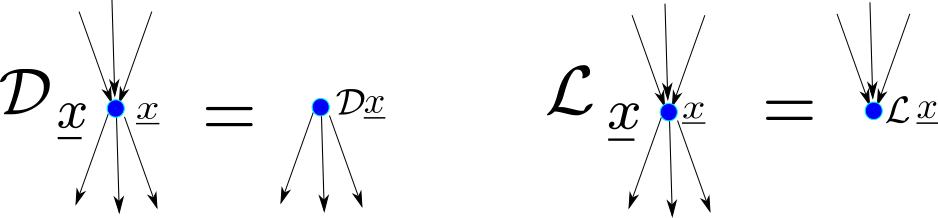
\includegraphics[width=4in]
{do-calc/do-rho-lam.png}
\caption{
The operator $\cald_\rvx$
converts node $\rvx$
into a root node $\cald \rvx$.
The operator $\call_\rvx$
converts node $\rvx$
into a leaf node $\call\rvx$.
} 
\label{fig-do-rho-lam}
\end{figure}


If
you don't
know yet
what we mean by a
a multi-node
$\rva.$, see
Chapter \nameref{ch-bnet-def}

Given a bnet
$G$,
we define
as follows
the operators
$\cald_{\rva.}$
and
$\call_{\rva.}$
for a multi-node
$\rva.$.

\beq
\cald_{\rva.}G =
\left[\prod_j \cald_{\rva_j}\right]G
\;,\;\;\;\;
\call_{\rva.}G =
\left[\prod_j \call_{\rva_j}\right]G
\;.
\eeq

Consider a bnet 
whose totality of nodes
is labeled $\rvX.$.
Recall that 

\beq
P(X.)=
\prod_j P(X_j|(X_k)
_{k:\rvX_k\in pa(\rvX_j)})
\;.
\eeq

Define an
operator $\cald$
that acts as follows\footnote{As usual,
$\caln(!x)$ denotes 
a constant 
that is independent of $x$.}: Let
$X.-a.=(X_k)_{k:\rvX_k\notin \rva.}$.

\beqa
P(X.-a.|\cald\rva.=a.)
&=&
\caln(!(X.-a.))
\frac{P(X.)}
{
\prod_{j:\rvX_j\in \rva.}
P(X_j|(X_k)
_{k:\rvX_k\in pa(\rvX_j)})
}
\\
&=&
\caln(!(X.-a.))
\prod_{j:\rvX_j\notin \rva.}
P(X_j|(X_k)
_{k:\rvX_k\in pa(\rvX_j)})
\\
&\neq&
P(X.-a.|\rva.=a.)
\;.
\eeqa
Also,

\beq
P(X.-a.,\cald\rva.=a.')=
P(X.-a.|\cald\rva.=a.)
\delta(a'., a.)
\;.
\eeq
In words, we replace
the TPM for 
multinode
$\rva.$ by
a deterministic
prior
distribution.

For instance, for the bnet

\beq
\xymatrix{
\rvx\ar[r]&\rvy
}
\eeq
with 

\beq
P(x,y)=P(y|x)P(x)
\;,
\eeq
one has 

\beq
P(y|\cald\rvx=x)=P(y|x)
\eeq
and

\beq
P(x|\cald \rvy=y)=P(x)
\;.
\eeq
This means that $\rvx$ causes $\rvy$
and $\rvy$ does not cause $\rvx$.

For the bnet

\beq
\xymatrix{
\rvc\ar[d]\ar[rd]
\\
\rvx\ar[r]&\rvy
}
\eeq
with 

\beq
P(x,y, c)=P(y|x, c)P(x|c)P(c)
\;,
\eeq
one has 

\beq
P(y, c|\cald\rvx=x)=P(y|x, c)P(c)
\;.
\eeq
Hence,

\beq
P(y|\cald\rvx=x)=\sum_c P(y|x,c)P(c)
\;.
\eeq
This is called {\bf adjusting the parents
of $\rvx$}.

For
$\rvb.\subset \rvX.-\rva.$,
define

\beq
P(b.|\cald\rva. =a.)=
\sum_{X.-a.-b.}
P(X.-a.|\cald\rva.=a.)
\;,
\eeq
and for
$\rvs.\subset \rvX.-\rva.-\rvb.$,
define

\beq
P(b.|\cald \rva.=a., s.)=
\frac{P(b., s.|\cald\rva.=a.)}
{P(s.|\cald\rva.=a.)}
\;.
\eeq

$P(b.|\cald \rva.=a., s.)$
is usually denoted instead  by
$P(b.|do(\rva.=a.), s.)$.
I prefer to 
use $\cald$
instead of $do()$.
I'll still call $\cald$
a {\bf do operator}. 

In $P(y|\cald \rvx=x)$,
node $\rvx$ is turned 
into a root node. This guarantees
that there is
no confounding node
connecting $\rvx$ and
$\rvy$. Such 
confounding nodes 
are unwelcomed 
when calculating
causal effects
between 
the 2 variables $\rvx$ and $\rvy$
 because they 
 introduce 
non-causal
correlations between
the two.
This is also 
what happens
in a {\bf Randomized 
Controlled Trial (RCT)}.
In a RCT
 with treatment $\rvx$,
the value
of $\rvx$ for each patient
is determined by a coin toss,
effectively
turning $\rvx$ into a root node.
Hence, the do operator mimics a RCT.


$P(b.|\cald \rva.=a., s.)$
is said to be {\bf identifiable}
(i.e., expressible without do())
if it can be
expressed in terms of
probability distributions
that only
depend on observed 
variables, and that
have no do operators
in them. 

For example,
if $\rvy$ has only one parent,
namely $\rvx$, then $P(y|x)$ is a TPM
of the bnet, so $P(y|\cald\rvx=x)=P(y|x)$.
Thus, in general, if $\rvy$ has only
one parent, $P(y|\cald\rvx=x)$ is 
identifiable. On the other hand, if
$\rvy$ has two parents, $\rvx$ and $\rva$, then
$P(y|x,a)$, not $P(y|x)$,
is the TPM for node $\rvy$,
so we will need more than the TPM
of node $\rvy$ to calculate $P(y|\cald\rvx=x)$.
So if $\rvy$ has more parents than node $\rvx$,
then the identifiability of $P(y|\cald\rvx=x)$
is not guaranteed.

 
As a second example,
$P(y|\cald\rvx=x)$ is identifiable
for the bnet

\beq
\xymatrix{
\rvz\ar[d]\ar[dr]
\\
\rvx\ar[r]&\rvy
}
\eeq
but it is not identifiable for the bnet

\beq
\xymatrix{
*++[F-o]{\rvz}\ar[d]\ar[dr]
\\
\rvx\ar[r]&\rvy
}
\eeq


For $\rvx, \rvy\in \bool$,
 the {\bf average controlled effect (ACE)}
is defined as

\beq
ACE=
P(y=1|\cald \rvx=1)-
P(y=1|\cald \rvx=0)
\eeq
and the 
{\bf Risk Difference (RD)} as

\beq
RD=
P(y=1|\rvx=1)-
P(y=1|\rvx=0)
\;.
\eeq

\section{Parent Adjustment Formula}


Suppose 
that $\rvx., \rvy., \rvz.$
are disjoint multinodes
and their union equals
 the
totality of all nodes of
a bnet. 
Suppose we have data
available that allows us  to
estimate $P(x., y., z.)$.
Hence, all nodes of the bnet
are observable.
Furthermore,
suppose $\rvz.=pa(\rvx.)$.
In other words,
we are 
considering the bnet

\beq
\xymatrix{
\rvz.\ar[d]\ar[dr]
\\
\rvx.\ar[r]&\rvy.
}
\;.
\eeq

Then

\beq
P(y., z.|\cald \rvx.=x.)
=P(y.|x., z.)P(z.)
\eeq
so

\beq
P(y.|\cald \rvx.=x.)
=\sum_{z.}P(y.|x., z.)P(z.)
\;.
\eeq
This is called
{\bf adjusting the parents}
of $\rvx.$.


We say that 
we are {\bf adjusting 
or controlling a variable $\rva$}
if we condition 
a probability on $\rva$ and 
then we average 
that probability over $\rva$.
More generally, 
we can adjust a whole
multinode $\rva.$ together.

Later on,
we will introduce 
a generalization
of 
this parent adjustment formula
called the 
backdoor adjustment formula.
In a backdoor adjustment formula,
the adjusted multinode
is not necessarily
 the parents of $\rvx.$, 
and $P(x., y., z.)$
need not represent the
whole bnet.



\section{3 Rules of Do Calculus}
Throughout 
this section, suppose
$\rva., \rvb., \rvr., 
\rvs.$ are disjoint
multinodes in a bnet $G$.


Recall
from Chapter \ref{ch-dsep}
on d-separation,
that  $(\rvb.\perp_G \rva.|\rvr., \rvs.)$
means that 
we have established
from the d-separation
rules that 
that all 
paths in $G$
 from
$\rva.$ to
$\rvb.$
are blocked
if we condition
on $\rvr.\cup \rvs.$.
Recall also that:

\begin{itemize}
\item {\bf Rule 0:} Insertion or
 deletion of
 observations, without
do operators.
($\rva.=a. \leftrightarrow 1$ )

\rulezero
$$
\rulezeropic
$$

\end{itemize}

The 3 rules of Do Calculus
can be presented in the same
format. 


\begin{itemize}
\item {\bf Rule 1:} 
Insertion or deletion of
 observations 
($\rva.=a. \leftrightarrow 1$ )

\ruleone
$$
\ruleonepic
$$


\item {\bf Rule 2:} Action or 
observation exchange 
($\cald \rva.=a. \leftrightarrow \rva.=a.$)

\ruletwo
$$
\ruletwopic
$$

\item {\bf Rule 3:} Insertion and
 deletion of actions
($\cald \rva.=a. \leftrightarrow 1$)

\rulethree
$$
\rulethreepic
$$


\end{itemize}

These rules have been
proven to be 
sufficient
for removing
all do operators
from an expression
for 
which it 
is possible to do so.

Next we discuss
two theorems that can be
proven using
Do Calculus:
the backdoor and the
front-door
adjustment formulae.

The 
backdoor theorem 
adjusts one multinode
and the 
front-door theorem adjusts two.


\section{Backdoor Adjustment Formula}

See Chapter \ref{ch-bdoor}
for examples of the use of the 
backdoor adjustment formula.
In this section,
we shall mainly be
concerned with
proving this
theorem
using Do Calculus.

For any two
disjoint
multinodes $\rvx.$
and $\rvy.$,
we define a {\bf backdoor path}
from $\rvx.$ to $\rvy.$
as a path from $\rvx.$
and $\rvy.$ that
starts with an arrow pointing into 
$\rvx.$,

\bdoordef

{\bf Motivation for BD criterion}: 
Part 1 rules out
paths 
from $\rvx$
to $\rvy$
containing a fork node (confounder)
which, if not blocked by conditioning on $\rvz.$, 
 would introduce a
non-causal correlation 
(confounder bias).
Part 2 rules out
a directed path
from $\rvx$ to $\rvy$
that has a mediator node
blocked by conditioning on $\rvz.$
or a collider node
unblocked by conditioning on $\rvz.$.



\begin{claim} Backdoor Adjustment Formula

\bdoorclaim
\end{claim}
\proof

For simplicity,
let us omit
the dots from the
multinodes.
If
$z$
satisfies the
backdoor
criterion
relative
to
$(\rvx, \rvy)$,
then
$\rvx, \rvy, \rvz$
must 
have the following 
structure.


\beq
\xymatrix{
{\rvz}\ar[d]\ar[rd]
\\
\rvx\ar[r]&\rvy
}
\eeq
\\
{\bf * Short proof:}
\begin{longtable}{l}
\color{red}
$P(y|\cald\rvx=x)=\sum_z
 P(y|\cald \rvx=x, z)P(z|\cald\rvx =x)$
\\
$\xymatrix{
\sum z\ar[dr]
\\
\cald \rvx=x\ar[r]
&y
}
\xymatrix{\\=}
\xymatrix{
\sum z\ar[dr]
\\
\cald \rvx=x\ar[r]\ar[u]
&y
}
$
\\
\color{red}
$=\sum_z P(y|x,z)P(z|\cald\rvx=x)$
\\
\xymatrix{\\=}
\xymatrix{
\sum z\ar[dr]
\\
\cald \rvx=x\ar[u]
&y
\\x\ar[ur]
}
\begin{tabular}{l}
\\
\\
by Rule 2
\end{tabular}
\\
\color{red}
$=\sum_z P(y|x,z)P(z)$
\\
\xymatrix{\\
=}
\xymatrix{
\sum z\ar[dr]
\\
x\ar[r]
&y
}
\begin{tabular}{l}\\
\\
by Rule 3.
\\
No info transmission\\
between $\cald\rvx$ and $\rvz$.
\end{tabular}
\end{longtable}


{\bf * Long proof:}
\begin{longtable}{l}
\color{red}
$P(y|\cald\rvx=x)
=
\sum_z
P(y|\cald\rvx=x, z)
P(z|\cald\rvx=x)$
\\
\quad by Probability Axioms
\\
=\color{red}
$\sum_z 
P(y|x, z)
P(z|\cald\rvx=x)$
\\
\quad $P(y|\cald \rvx=x, z)\rarrow
P(y|x, z)$
\\
\quad  by Rule 2: $\ruletwopic$
\\
\quad  in
$\call_\rvx G:
\xymatrix{
{z}\ar[d]\ar[rd]
\\
\cald \rvx=x
&y
}
\xymatrix{\\=}
\xymatrix{
{z}\ar[d]\ar[rd]
\\
x
&y
}
$
\\ 
=\color{red}
$\sum_z 
P(y|x, z)
P(z)$
\\
\quad $P(z|\cald \rvx=x)\rarrow
P(z)$
\\
\quad  by Rule 3: $\rulethreepic$
\\
\quad in
$\cald_\rvx G:
\xymatrix{
{z}\ar[rd]
\\
\cald\rvx=x\ar[r]
&y
}\xymatrix{\\=}
\xymatrix{
{z}\ar[rd]
\\
&y
}
$
\end{longtable}
.\qed

Note that the backdoor adjustment  formula
can be written as
 
\beqa
P(y.|\cald \rvx. =x.)
&=&
\sum_{z.}P(y.|x., z.)P(z.)
\\
&=&
\sum_{z.}\frac{P(y.,x., z.)}
{P(x.|z.)}
\eeqa
This assumes $P(x.|z.)\neq 0$
for all $x., z.$. This assumption
is referred to
as {\bf positivity},
and is violated
if $P(x.|z.)=\delta(x., x.(z.))$.
$P(x.|z.)$ is called the 
{\bf propensity score}
of $x.$ given $z.$.
This
equation does 
{\bf inverse probability weighting}.
One
can approximate $P(x.|z.)$ 
in this equation
to get
an approximation
to  $P(y|\cald\rvx=x)$.


\section{Front Door Adjustment Formula}
See Chapter \ref{ch-fdoor}
for examples of the use of the 
front-door adjustment formula.
In this section,
we shall mainly be
concerned with
proving this
theorem
using Do Calculus.

\fdoordef

\begin{claim} Front-Door Adjustment
Formula

\fdoorclaim

\end{claim}
\proof

(See also Ref.\cite{pearl-front-door}
for a proof
of the Front-Door Adjustment Formula
without 
using Do Calculus.)

For simplicity,
let us omit
the dots from the
multinodes.
If
$\rvm$
satisfies the
front-door
criterion
relative
to
$(\rvx, \rvy)$,
then
$\rvx, \rvm, \rvy$
must 
have the following 
structure,
where
node $\rvc$
is hidden. 


\beq
\xymatrix{
&*++[F-o]{\rvc}\ar[ld]\ar[rd]
\\
\rvx\ar[r]&\rvm\ar[r]&\rvy
}
\eeq
{\bf * Short proof:}
\begin{longtable}{l}
$\color{red}
P(y|\cald\rvx=x)=
\sum_m 
P(y|\cald\rvx=x, m)
P(m|\cald\rvx=x)$
\\
\\
\xymatrix{
&*++[F-o]{\sum c}\ar[rd]
\\
\cald \rvx=x\ar[r]
&\sum m\ar[r]
&y
}
\xymatrix{\\=}
\xymatrix{
&
\\
\cald \rvx=x\ar[r]\ar@/_1.2pc/[rr]
&\sum m\ar[r]
&y
}
\\
\\
$\color{red}=
\sum_m 
P(y|\cald\rvx=x, \cald\rvm=m)
P(m|\cald\rvx=x)$
\\
\xymatrix{\\=\sum_m }
\xymatrix{
\cald \rvx=x\ar[r]\ar@/_1.2pc/[rr]
&m&y
\\
&\cald\rvm=m\ar[ru]
}
\begin{tabular}{l}
\\
by Rule 2
\end{tabular}
\\
$\color{red}=
\sum_m 
P(y|\cald\rvx=x, \cald\rvm=m)
P(m| x)$
\\
\xymatrix{\\=\sum_m }
\xymatrix{
\cald\rvx=x\ar@/_1pc/[rr]
&m
&y
\\
x\ar[ru]
&\cald\rvm=m\ar[ru]
}
\begin{tabular}{l}
\\
by Rule 2
\end{tabular}
\\
$\color{red}=
\sum_m 
P(y|\cald\rvm=m)
P(m|x)$
\\
\xymatrix{\\=\sum_m }
\xymatrix{
&m
&y
\\
x\ar[ru]
&\cald\rvm=m\ar[ru]
}
\begin{tabular}{l}
\\
by Rule 3.\\
No info transmission\\
between $\cald\rvx$ and $\rvy$\\
if condition on $\cald \rvm$.
\end{tabular}
\\
$\color{red}=
\sum_{x'}
\sum_m 
P(y|\cald\rvm=m, x')
P(x'|\cald\rvm=m)
P(m|x)$
\\
\xymatrix{\\=\sum_m}
\xymatrix{
&m
&y
\\
x\ar[ru]
&\cald\rvm=m\ar[ru]\ar[r]
&\sum x'\ar[u]
}
\\
$\color{red}=
\sum_{x'}
\sum_m 
P(y|m, x')
P(x'|\cald\rvm=m)
P(m|x)$
\\
\xymatrix{\\=\sum_m}
\xymatrix{
&m\ar[r]
&y
\\
x\ar[ru]
&\cald\rvm=m\ar[r]
&\sum x'\ar[u]
}
\begin{tabular}{l}
\\
by Rule 2
\end{tabular}
\\
$\color{red}=
\sum_{x'}
\sum_m 
P(y|m, x')
P(x')
P(m|x)$
\\
\xymatrix{\\=}
\xymatrix{
&\sum m\ar[r]
&y
\\
x\ar[ru]
&&\sum x'\ar[u]
}
\begin{tabular}{l}
\\
by Rule 3.
\\
No info transmission\\
between $\cald\rvm$ and $\rvx'$.
\end{tabular}
\end{longtable}



{\bf * Long proof:}
\begin{longtable}{l}
$\color{red}
P(y|\cald\rvx=x)=
\sum_m 
P(y|\cald\rvx=x, m)
P(m|\cald\rvx=x)$
\\
\quad by Probability Axioms
\\
$\color{red}=
\sum_m 
P(y|\cald\rvx=x, \cald\rvm=m)
P(m|\cald\rvx=x)$
\\
\quad $P(y|\cald\rvx=x, m)\rarrow
P(y|\cald\rvx=x, \cald m=m)$
\\
\quad by Rule 2: $\ruletwopic$
\\
\quad in $\call_\rvm\cald_\rvx G:$
$\xymatrix{
&*++[F-o]{c}\ar[rd]
\\
\cald \rvx=x\ar[r]
&\cald \rvm=m
&y
}
\xymatrix{\\=}
\xymatrix{
&*++[F-o]{c}\ar[rd]
\\
\cald\rvx=x\ar[r]&m&y
}$
\\
$\color{red}=
\sum_m 
P(y|\cald\rvx=x, \cald\rvm=m)
P(m| x)$
\\
\quad $P(m|\cald\rvx=x)\rarrow P(m|x)$
\\
\quad by Rule 2: $\ruletwopic$
\\
\quad in $\call_\rvx G:$
$\xymatrix{
&*++[F-o]{c}\ar[ld]\ar[rd]
\\
\cald\rvx=x&m\ar[r]&\rvy
}
\xymatrix{\\=}
\xymatrix{
&*++[F-o]{c}\ar[ld]\ar[rd]
\\
x&m\ar[r]&\rvy
}$
\\
$\color{red}=
\sum_m 
P(y|\cald\rvm=m)
P(m|x)$
\\
\quad $P(y|\cald\rvx=x, \cald\rvm=m)
\rarrow
 P(y|\cald\rvm=m)$
\\
\quad by Rule 3: $\rulethreepic$
\\
\quad 
 in 
$\cald_\rvx\cald_\rvm G:$
$\xymatrix{
&*++[F-o]{c}\ar[rd]
\\
\cald\rvx=x&\cald\rvm=m\ar[r]&\rvy
}\xymatrix{\\=}
\xymatrix{
&*++[F-o]{c}\ar[rd]
\\
&m\ar[r]&\rvy
}
$
\\
$\color{red}=
\sum_{x'}
\sum_m 
P(y|\cald\rvm=m, x')
P(x'|\cald\rvm=m)
P(m|x)$
\\
\quad by Probability Axioms
\\
$\color{red}=
\sum_{x'}
\sum_m 
P(y|m, x')
P(x'|\cald\rvm=m)
P(m|x)$
\\
\quad $P(y|\cald\rvm=m, x')
\rarrow
\quad P(y|m, x')$
\\
\quad by Rule 2: $\ruletwopic$
\\
\quad
in 
$\call_\rvm G:$
$\xymatrix{
&*++[F-o]{c}\ar[rd]\ar[ld]
\\
x\ar[r]
&\cald\rvm= m
&y
}
\xymatrix{\\=}
\xymatrix{
&*++[F-o]{c}\ar[rd]\ar[ld]
\\
x\ar[r]
& m
&y
}
$
\\
$\color{red}=
\sum_{x'}
\sum_m 
P(y|m, x')
P(x')
P(m|x)$
\\
\quad $P(x'|\cald\rvm=m)
\rarrow
P(x')$
\\
\quad by Rule 3: $\rulethreepic$
\\
\quad
 in 
$\cald_\rvm G:$
$\xymatrix{
&*++[F-o]{c}\ar[rd]\ar[ld]
\\
x
&\cald\rvm=m\ar[r]
&y
}
\xymatrix{\\=}
\xymatrix{
&*++[F-o]{c}\ar[rd]\ar[ld]
\\
x
&m\ar[r]
&y
}
$
\end{longtable}
.\qed

\section{Do operator for DEN diagrams}

Recall that
the structural
equations
for a linear DEN, as
given
by Eq.(\ref{eq-mat-fully-conn})
of Chapter \ref{ch-linear-sys}, are:

\beq
\rvx=A\rvx +\rvu
\;.
\label{eq-struc-pre-rho}
\eeq
Therefore,

\beq
\rvx=(1-A)^{-1}\rvu
\eeq
which
can be 
represented for
both linear
and non-linear DEN
diagrams by:

\beq
\rvx_i = x_i(\rvu.)
\eeq 

If now
we apply the
operator
$\cald_{\rva=a}$
to 
the diagram
described by
the structural
equations Eqs.\ref{eq-struc-pre-rho},
we get the following
new
structural
equations:

\beq
\rvx^*_i =\left\{
\begin{array}{lll}
 \sum_{j<i} A_{i|j}\rvx^*_j + \rvu_i&
 \text{if $\rvx_i\neq \rva$}
\\
a&
\text{if $\rvx_i=\rva$}
\end{array}
\right.
\label{eq-ith-struc-post-rho}
\;,
\eeq
where we are
calling 
$\rvx^*_i$ the
nodes
of the DEN 
diagram post intervention.

Eqs.(\ref{eq-ith-struc-post-rho})
can be expressed in matrix notation
as follows.
Define $\pi_\rva$ to
be the $nx\times nx$ matrix 
with all entries equal
to  zero
except for the $(i_0,i_0)$ entry, which is 1.
And define $e_\rva$
to be the column vector
with all entries zero
except for the $i_0$'th one, 
which is 1. 
Here
$i_0$  
is
defined so that $\rvx_{i_0}=\rva$.
In other words, $\pi_\rva$ and $e_\rva$
are defined by

\beq
(\pi_\rva)_{i,j}= \indi(i=j, \rva=\rvx_i)
\;
\eeq
and

\beq
(e_\rva)_i=\indi(\rva=\rvx_i)
\;,
\eeq
for $i, j\in \{0, 1, \ldots, nx-1\}$.
Next define

\beq
\pi_{!\rva}=1-\pi_\rva
\;,
\eeq

\beq
A^*=\pi_{!\rva} A
\;,
\eeq
and

\beq
\rvu_{!\rva}=\pi_{!\rva} \rvu
\;.
\eeq
The effect
of pre-multiplying
the matrix
$A$ 
and the column vector $\rvu$ by
$\pi_{!\rva}$
is to leave all rows
intact except for
the $i_0$
row, which is set to zero. Here
 $i_0$ is defined by
 $\rva=\rvx_{i_0}$.
Finally,
using 
all
of the
variables just defined,
we can express the
structural equations
of the linear DEN diagram,
post intervention, as


\beq
\rvx^*= A^* \rvx^* + \rvu_{!\rva} +
ae_\rva
\;.
\eeq
Thus,

\beq
\rvx^*=(1-A^*)^{-1} (\rvu_{!\rva}+ae_\rva)
\;.
\eeq
which
can be 
represented for
both linear
and non-linear DEN
diagrams by:

\beq
\rvx^*_i=x^*_i(\rvu_{!\rva},a)
\;.
\eeq



For any bnet,

\beq
P(\rvy=y|\rvx=x)
=
P_{G}(\rvy=y|\rvx=x)
\eeq

\beq
P(\rvy=y|\cald\rvx=x)
=
P_{\cald_{\rvx=x}G}(\rvy=y)
\eeq


\begin{claim}
For a non-linear DEN diagram,



\beq
P(y|\cald\rvx=x)=
E\left[
\delta[y, y(\rvu_{!\rvx},x)]\right]
\;.
\eeq
\end{claim}
\proof
\beqa
P(\rvy=y|\cald\rvx=x)
&=&
P_{\cald_{\rvx=x}G}(\rvy=y)
\\
&=&\sum_{u_{!\rvx}}P(u_{!\rvx})
P_{\cald_{\rvx=x}G}
(\rvy=y|u_{!\rvx})
\\
&=&\sum_{u_{!\rvx}}P(u_{!\rvx})
\delta[y, y(u_{!\rvx},x)]
\\
&=&
E_{\rvu_{!\rvx}}
[\delta[y, y(u_{!\rvx}, x)]]
\\
&=&
E[\delta[y,y(\rvu_{!\rvx}, x)]]
\eeqa
\qed

\begin{claim}
For a nonlinear DEN diagram,

\beq
E[\rvy|\cald \rvx=x]=
E[y(\rvu_{!\rvx}, x)]
\;.
\eeq
\end{claim}
\proof

\beqa
E[\rvy|\cald \rvx=x]
&=&
\sum_{y}
yP(\rvy=y|\cald\rvx=x)
\\
&=&
\sum_{y}
yE[
\delta[y, y(u_{!\rvx},x)]]
\\
&=&
E[y(\rvu_{!\rvx}, x)]
\eeqa
\qed


For any bnet
\beqa
P(y|\cald\rvx=x, z)&=&
\frac{P(y, z|\cald\rvx=x)}
{P(z|\cald\rvx=x)}
=
P_{\cald_{\rvx=x}G}(y|x, z)
\eeqa

For a nonlinear DEN diagram,
\beq
P(y, z|\cald\rvx=x)
=
\sum_{u_{!\rvx}}P(u_{!\rvx})
\delta[y, y(u_{!\rvx},x)]
\delta[z, z(u_{!\rvx},x)]
\eeq

\beq
P(z|\cald\rvx=x)=
\sum_{u_{!\rvx}}P(u_{!\rvx})
\delta[z, z(u_{!\rvx},x)]
\;.
\eeq

\chapter{Do Calculus proofs}
\label{ch-do-calc-proofs}

In Chapter \ref{ch-do-calc},
we explained Do Calculus,
but referred to this
chapter for proofs
of claims that
use Do Calculus.
In this chapter, we've
aggregated
 all proofs, from
throughout the book,
of claims that use Do Calculus.

Note that even though the 3
rules of Do Calculus
are great for proving
adjustment formulae
for general classes of DAGs,
they are sometimes overkill
for proving
 adjustment formulae
for a single specific DAG.
Indeed, since the
 3 rules of Do Calculus
are a consequence
of the d-separation theorem, it follows that
all adjustment
formulae should be
provable from first principles,
assuming only
the d-separation theorem
and the standard rules of
probability theory.
In this chapter, we present
a technique that allows us to do just that: prove 
adjustment formulae from first principles,
without using the 
3 Rules of Do Calculus.


In this chapter, we use the
 following conventions for bnet diagrams.

\bnetInstantiations

\hiddenNodes

\selectionGraphs

We often write

\beq
\begin{array}{c}
P(a)\xymatrix {a\ar[r]&\sum b\ar[r]&c}
\quad=\quad
P(a) \xymatrix {a\ar[r]&c}
\\
\sum_b P(c|b)P(b|a)P(a)=P(c,a)
\label{eq-promi-dep}
\end{array}
\eeq
because  the left hand side summed over $a,c$ yields 1. However,
this equation
is only true if the $P(c,a)$
on the right hand side
assumes a particular promise, namely
\beq
P(c,b, a)=P(c|b)P(b|a)P(a)
\eeq
An alternative way of saying the same thing
is to say that Eq.(\ref{eq-promi-dep})
 assumes that $P()=P_G()$ where 
$G$ is the bnet $\rva\rarrow\rvb\rarrow\rvc$.
We say that Eq.(\ref{eq-promi-dep})
is {\bf bnet promise dependent}.


Next we will
give some {\bf node summation identities}
that are used in this chapter.
Note that these identities are {\bf bnet promise independent}; i.e., they are true
for any bnet promise. 

\hrule
\begin{enumerate}
\item

\beq
\sum_a
P(a|x_1, x_2)=1
\eeq

\beq
\xymatrix@R=.3pc{
x_1\ar[dr]
\\
&\sum a&=1
\\
x_2\ar[ur]
}
\label{eq-collider-sum}
\eeq
\hrule
\item
\beq
\sum_a P(y|a, x_1, x_2)P(a|x_1, x_2)P(x_2|x_1)P(x_1)
= P(y,x_1, x_2)
\;.
\eeq

\beq
\xymatrix{\\P(x_1)}
\xymatrix{
x_1\ar[rd]\ar[drr]\ar[dd]
\\
&\sum a\ar[r]
&y
\\
x_2\ar[ru]\ar[rru]
}
\xymatrix
{\\ =P(x_1)}
\xymatrix{
x_1\ar[rrd]\ar[dd]
\\
&&y
\\
x_2\ar[urr]
}
\label{eq-univ-bdoor}
\;.
\eeq
This identity can be interpreted
geometrically by noting that the 
bnet on the left hand side (LHS) is fully connected 
so one can reverse the direction of the 
arrow from $\sum a \rarrow y$ without changing the numerical value of the LHS. Then the sum over $a$
yields 1 so the $\sum a$ vertex 
with its 3 incoming arrows can be deleted.

The following identity has a similar geometrical interpretation

\beq
\sum_a P(y|x_2, a, x_1)P(x_2|a, x_1)P(x_1|a)P(a)
= P(y,x_1, x_2)
\;.
\eeq

\beq
\xymatrix{
x_1\ar[drr]\ar[dd]
\\
&\EE a\ar[r]\ar[ul]\ar[dl]
&y
\\
x_2\ar[rru]
}
\xymatrix
{\\ = P(x_1)}
\xymatrix{
x_1\ar[rrd]\ar[dd]
\\
&&y
\\
x_2\ar[urr]
}
\label{eq-univ-bdoor-ee}
\;.
\eeq


\hrule
\item
\beq
\sum_a P(y|a, x)P(a|x)P(x)=P(x,y)
\eeq

\beq
\xymatrix@R=1pc{
\\P(x)}
\xymatrix@R=1pc{
&\sum a\ar[rd]
\\
x\ar[ru]\ar[rr]
&&y
&=&P(x)\quad
x\ar[r]
&y}
\label{eq-med-sum}
\eeq
Once again, the bnet on the LHS is fully
connected so the arrow $\sum a\rarrow y$ can be reversed and then the sum over $a$ yields 1.

The following identity has a similar geometrical interpretation

\beq
\sum_a P(y|x,a)P(x|a)P(a)=P(x,y)
\eeq

\beq
\xymatrix@R=1pc{
&\EE a\ar[rd]\ar[ld]
\\
x\ar[rr]
&&y
&=&P(x)\quad
x\ar[r]
&y}
\label{eq-med-sum-ee}
\eeq

\hrule

\item
\beq
\sum_a P(y|a)P(a)=P(y)
\eeq

\beq
\xymatrix{
\EE a\ar[r]
&y
&=&P(y)
}
\label{eq-diff-priors}
\eeq
Furthermore,

\beq
\sum_a P(a|y)P(y)=P(y)
\eeq

\beq
\xymatrix{
P(y)\quad
\sum a
&y\ar[l]
&=&P(y)
}
\label{eq-diff-priors-ee}
\eeq

\end{enumerate}
\hrule

The moral of the above summation identities is that
if one has a fully connected bnet, or a bnet clique
(i.e., fully connected subgraph of a bnet)\footnote{Note that in order to use the node summation identities on a clique,
the clique's nodes can have NO incoming arrows (i.e., arrows pointing from outside the clique into the clique). Outgoing arrows are allowed though. I like to call such a clique an {\bf exploding clique}, because of its outgoing arrows.},
one can remove completely (including its arrows) a sum vertex $\sum a$ or an average
vertex $\EE a$ of the clique. Not only that! We can also 
replace a sum vertex $\sum a$  of the clique by a different  sum vertex $\sum b$. Likewise, we can replace
an average vertex $\EE a$  of the clique by a different  average vertex $\EE b$.

%An important caveat concerning the above
%summation identities is that 
%the instantiations that they produce depend on the
%original bnet whence they come from. 
%This caveat is illustrated in Fig.\ref{fig-dep-on-origing-bnet}.
%This caveat is especial relevant when dealing 
%with do operators. In that case, the unamputated
%graph and the amputated graph are different bnets, with
%different promises.
%
%\begin{figure}[h!]
%$$
%\begin{array}{c|c}
%\sum_a P_{G}(x_2|a)P_{G}(a|x_1)=P_{G}(x_2|x_1)
%&
%\sum_a P_{G'}(x_2|a, x_1)P_{G'}(a|x_1)=P_{G'}(x_2|x_1)
%\\
%\xymatrix@C=1.5pc{
%x_1\ar[r]
%&\sum a\ar[r]
%&x_2
%&=&
%x_1\ar[r]
%&x_2}
%&
%\xymatrix@C=1.5pc{
%x_1\ar[r]\ar@/_1pc/[rr]
%&\sum a\ar[r]
%&x_2
%&=&
%x_1\ar[r]
%&x_2}
%\end{array}
%$$
%\caption{Note that there are cases when $P_G(x_2|x_1)
%\neq P_{G'}(x_2|x_1)$. Hence,
% $P(x_2|x_1)$ depends on the bnet of origin.
%}
%\label{fig-dep-on-origing-bnet}
%\end{figure}
%
%




We define a {\bf do-adjustment formula}
for {\bf do-query}
$P(y|\cald\rvx=x)$
to be an algebraic expression  
constructed from the TPMs for {\it observed} (i.e., not hidden) nodes of the original bnet $G$.
If a do-adjustment formula
exists for a
particular do-query,
then we say the do-query is
 {\bf do-identifiable (DI)}.
% \footnote{
%To prove that a do-query $P(y|\cald\rvx=x, z)$
%is do-identifiable
%for a graph $G$,
%just prove that $\rvy\perp\rvx|\rvz$
%in $\call_\rvx G$.
%This is called Rule 2 of Do Calculus,
%but it is easy to understand just from
%the d-separation theorem.
%Info can be transmitted
%between $\rvy$ and $\rvx$ by
%either (1) paths
%in $\cald_\rvx G$
%or (2) paths in $\call_\rvx G$.
%$P(y|\cald\rvx=x, z)=
%P(y|x, z)$
%means the info is being transmitted only
%by (1).
%So the Rule 2 premise is checking
%that no info is being transmitted
%by (2). }
A {\bf do-transfer formula}
is a relationship between 2  do-queries.
This chapter deals with both
do-adjustment and do-transfer
formulae.

Let $G$ be a graph before
amputation
of the arrows entering node $\rvx$,
and let $G_{amp(x)}=\cald_{\rvx=x}G$
be the same graph after amputation
at $\rvx$.
Also let $P_G()$ be
the promise
for graph $G$, and $P_{G_{amp(x)}}()$
be that for $G_{amp(x)}$.
In general, the
following is always true,
for bnets
with or bnets without hidden nodes:\footnote{Note that $P_{G_{amp(x)}}(y|x)\neq P_G(y|x)$
in general.
In fact,
$P_{G_{amp(x)}}(y|x)= P_G(y|x)$
iff there is no confounding,
so $P_{G_{amp(x)}}(y|x)\neq P_G(y|x)$
indicates confounding.
}

\beq
P_{G_{amp(x)}}(y|\cald\rvx=x)=P_{G_{amp(x)}}(y|x)\neq P_G(y|x)
\;
\eeq
However, $P_{G_{amp(x)}}(y|x)$ is
not a valid adjustment formula
for this query
because it's not expressed in terms
of observed TPMs of $G$.

To make matters even more confusing, let $G|x$
be the bnet $G$ conditioned on $\rvx=x$. If $G$ has promise $P_G()$,
then  $P_{G|x)}(\cdot) = P_G(\cdot|x)$.
 
Note that, in general,  $P_G$, $P_{G_{amp(x)}}$ and $P_{G|x}$ are
different probability distributions. 

IMPORTANT: For any adjustment formula, we assume
a hypothesis bnet $G_{hypo}$.
Then for a query
$P(y|\cald\rvx=x)$, we express the adjustment
formula in terms of the promise $P()=P_{G_{hypo}|x}()=P_{G_{hypo}}(\cdot|x)$.


%Note that
%it's always true that $P(y|\cald \rvx = x)=P(y|x)$.
%However, if the bnet contains more nodes than just $\rvx$ and $\rvy$, then the bnet is identifiable
%iff it can be stratified (i.e., 
%expressed as $P(y|x)=\sum_{z.}P(y|x, z.)P(z.)$
%for some observed multinode $\rvz.$).
%Thus, an alternative  name for identifiability is
%{\bf stratifiability}. Note also that there mightt be more than
%one adjustment formula, but they must all 
%be numerically equal to $P(y|x)$ for all $x$ and $y$.


The following 2 step heuristic technique,
which I call the {\bf Not Do Calculus} (NDC) technique, appears to be equivalent to Pearl's 3 rules of Do Calculus.\footnote{This NDC technique was invented solely by me. I haven't proven that it is equivalent to Pearl's 
3 rules of Do Calculus. I believe it is,
but it might not be. It 
correctly produces the backdoor and frontdoor adjustment formulae.}

\begin{mdframed}[hidealllines=true,backgroundcolor=blue!10]

\begin{enumerate}
\item 
Write down a bnet instantiation
that has a DAG structure identical
to the DAG structure of $G$,
except that arrows entering node
$\rvx$ have been amputated.
All nodes  of that instantiation, except
nodes  $x$ and $y$,
are summed (indicated by $\sum$) or averaged
(indicated by $\EE$) over.



\item Use the node summation identities to
remove all sums and averages over hidden nodes.
Each sum or average over a hidden node may be 
removed completely or replaced by a sum or average over an observed node. 
\end{enumerate}
Perform these steps until you remove all sums and averages  over hidden variables 
and obtain a valid adjustment formula.
If such an outcome cannot be achieved,
declare the  query not-identifiable.

\end{mdframed}


\begin{figure}[h!]
$$
\begin{array}{ccc}
\xymatrix{
&\rvz\ar[ld]\ar[rd]
\\
\rvx\ar[rr]&&\rvy
}
&\quad\quad&
\xymatrix{
&*++[F-o]{\rvz}\ar[ld]\ar[rd]
\\
\rvx\ar[rr]&&\rvy
}
\\
(a) \text{$P(y|\cald\rvx=x)$ is DI}
&&(b) \text{$P(y|\cald\rvx=x)$ is not-DI}
\end{array}
$$
\caption{Examples of
bnets for which
the do-query $P(y|\cald\rvx=x)$
is
DI
and not-DI.
}
\label{fig-iden-noniden}
\end{figure}
See Fig.\ref{fig-iden-noniden}
for some simple
examples of
bnets for which
the do-query $P(y|\cald\rvx=x)$
is
DI
and not-DI.
Using the NDC technique,
we can easily see why the
query $P(y|\cald\rvx=x)$
is DI
for bnet $(a)$ 
and not-DI for bnet $(b)$
of Fig.\ref{fig-iden-noniden}.

For bnet $(a)$, after amputating arrow
$z\rarrow x$ and averaging over node $z$,
we get

\beqa
P(y|\cald\rvx=x)
&=&
\xymatrix{
\EE z\ar[dr]
\\
x\ar[r]
&y
}
\label{eq-simplest-identifiable}
\eeqa
The right hand
side of Eq.(\ref{eq-simplest-identifiable})
is a valid
adjustment formula
because it's expressed in terms
of observed TPMs of $G$.

For bnet $(b)$,
if we amputate arrow
$z\rarrow x$
and average over node $z$,
we get

\beqa
P(y|\cald \rvx =x)
&=&
\xymatrix{
*++[F-o]{\EE z}\ar[rd]
\\
x\ar[r]
&y
}
\label{eq-simplest-not-DI}
\eeqa
The right hand
side of Eq.(\ref{eq-simplest-not-DI})
is not a valid
adjustment formula
because
if we replace $\EE z$ by $\EE x' $, we get 
$\sum_{x'}P(y|x, x')P(x')$,
and $P(y|x, x')$ is undefined.






\begin{claim}
\label{cl-decBackDoor}
\decBackDoor
\end{claim}

\proof

{\bf * proof 1:}
%\beq
%P(y|\cald\rvx=x, z)
%=
%\xymatrix{
%z\ar[dr]
%\\
%x\ar[r]
%&y
%}
%\eeq

\beq
P(y|\cald\rvx=x)
=
\xymatrix{
\EE z\ar[dr]
\\
x\ar[r]
&y
}
\eeq


{\bf * proof 2:}
\begin{longtable}{l}
\color{red}
$P(y|\cald\rvx=x)
=
\sum_z
P(y|\cald\rvx=x, z)
P(z|\cald\rvx=x)$
\\
\quad by Probability Axioms
\\
\color{red}
$=\sum_z
P(y|x, z)
P(z|\cald\rvx=x)$
\\
\quad $P(y|\cald \rvx=x, z)\rarrow
P(y|x, z)$
\\
\quad  by Rule 2:
\ruletwoshort
\\
\quad
$\rvy\perp\rvx|\rvz$ in
$\call_\rvx\cald_\emptyset G:
\xymatrix{
\rvz\ar[d]\ar[rd]
\\
\rvx
&\rvy
}$
\\
\color{red}
$=\sum_z
P(y|x, z)
P(z)$
\\
\quad $P(z|\cald \rvx=x)\rarrow
P(z)$
\\
\quad  by Rule 3:
\rulethreeshort
\\
\quad
$\rvz\perp \rvx$ in
$\cald_\rvx \cald_\emptyset G:
\xymatrix{
\rvz\ar[rd]
\\
\rvx\ar[r]
&\rvy
}
$
\end{longtable}
\qed




\begin{claim}
\label{cl-decFrontDoor}
\decFrontDoor
\end{claim}

\proof


{\bf * proof 1:}

\begin{longtable}{l}
$P(y|\cald\rvx=x) =\sum_c\sum_m P(y|m,c)P(m|x)P(c)$
\\
\hspace{2cm}
\xymatrix{
&\EE c\ar[dr]
\\
x\ar[r]&\sum m\ar[r]
&y
}
\\
\quad$=\sum_m \left[\sum_c\frac{1}{P(m|c)} P(y|m,c)P(m|c)P(c)\right]P(m|x)$
\\
\hspace{2cm}
\xymatrix{\\
\sum_m\sum_c\frac{P(c)}{P(m|c)}
}
\xymatrix{
&&c\ar[dr]\ar[d]
\\
x\ar[r]&m&m\ar[r]
&y
}
\\
\quad$=\sum_m \frac{1}{P(m)}\left[\sum_c P(y|m,c)P(m|c)P(c)\right]P(m|x)$ \\
\hspace{2cm}(because $P(m|c)=P(m)$ by d-separation
on $G_{hypo}|x$)
\\
\hspace{2cm}
\xymatrix{\\
\sum_m\frac{1}{P(m)}
}
\xymatrix{
&&\EE c\ar[dr]\ar[d]
\\
x\ar[r]&m&m\ar[r]
&y
}
\\
\quad$=\sum_m P(y|m)P(m|x)$ 
\\
\hspace{2cm}
(because square bracketed expression equals $P(y,m)$)
\\
\hspace{2cm}
\xymatrix{
x\ar[r]&\sum m \ar[r]& y
}\quad (this simplifies frontdoor AF)
\\
\quad
$=\sum_{x'}\sum_m P(y|m,x')P(m|x)P(x')$
\\
\hspace{2cm}
(because can reverse steps that led to last expression)
\\
\hspace{2cm}
\xymatrix{
&\EE x'\ar[dr]
\\
x\ar[r]&\sum m\ar[r]
&y
}
\end{longtable}

{\bf * proof 2:}
\begin{longtable}{l}
$\color{red}
P(y|\cald\rvx=x)=
\sum_m
P(y|\cald\rvx=x, m)
P(m|\cald\rvx=x)$
\\
\quad by Probability Axioms
\\
$\color{red}=
\sum_m
P(y|\cald\rvx=x, \cald\rvm=m)
P(m|\cald\rvx=x)$
\\
\quad $P(y|\cald\rvx=x, m)\rarrow
P(y|\cald\rvx=x, \cald m=m)$
\\
\quad by Rule 2:
\ruletwoshort
\\
\quad $\rvy\perp \rvm|\rvx$ in
$\call_\rvm\cald_\rvx G:$
$\xymatrix{
&*++[F-o]{\rvc}\ar[rd]
\\
\rvx\ar[r]
&\rvm
&\rvy
}$
\\
$\color{red}=
\sum_m
P(y|\cald\rvx=x, \cald\rvm=m)
P(m| x)$
\\
\quad $P(m|\cald\rvx=x)\rarrow P(m|x)$
\\
\quad by Rule 2:
\ruletwoshort
\\
\quad
$\rvm\perp \rvx$ in
$\call_\rvx\cald_\emptyset G:$
$\xymatrix{
&*++[F-o]{\rvc}\ar[ld]\ar[rd]
\\
\rvx
&\rvm\ar[r]
&\rvy
}$
\\
$\color{red}=
\sum_m
P(y|\cald\rvm=m)
P(m|x)$
\\
\quad $P(y|\cald\rvx=x, \cald\rvm=m)
\rarrow
 P(y|\cald\rvm=m)$
\\
\quad by Rule 3:
\rulethreeshort
\\
\quad
$\rvy\perp\rvx|\rvm$ in
$\cald_\rvx\cald_\rvm G:$
$\xymatrix{
&*++[F-o]{\rvc}\ar[rd]
\\
\rvx
&\rvm\ar[r]
&\rvy
}$
\\
$\color{red}=
\sum_{x'}
\sum_m
P(y|\cald\rvm=m, x')
P(x'|\cald\rvm=m)
P(m|x)$
\\
\quad by Probability Axioms
\\
$\color{red}=
\sum_{x'}
\sum_m
P(y|m, x')
P(x'|\cald\rvm=m)
P(m|x)$
\\
\quad $P(y|\cald\rvm=m, x')
\rarrow
\quad P(y|m, x')$
\\
\quad by Rule 2:
\ruletwoshort
\\
\quad
$\rvy\perp\rvm|\rvx$ in
$\call_\rvm \cald_\emptyset G:$
$\xymatrix{
&*++[F-o]{\rvc}\ar[rd]\ar[ld]
\\
\rvx\ar[r]
&\rvm
&\rvy
}$
\\
$\color{red}=
\sum_{x'}
\sum_m
P(y|m, x')
P(x')
P(m|x)$
\\
\quad $P(x'|\cald\rvm=m)
\rarrow
P(x')$
\\
\quad by Rule 3:
\rulethreeshort
\\
\quad
$\rvx\perp\rvm$ in
$\cald_\rvm \cald_\emptyset G:$
$\xymatrix{
&*++[F-o]{\rvc}\ar[rd]\ar[ld]
\\
\rvx
&\rvm\ar[r]
&\rvy
}$
\end{longtable}
\qed



\begin{claim}
\label{cl-decNapkin}
\decNapkin
\end{claim}
\proof
\\
\begin{align}
P(y|\cald\rvx=x)
&=
\xymatrix{
&*++[F-o]{\EE u_1}\ar[ddl]\ar[ddrr]
&&
\\
&*++[F-o]{\EE u_2}\ar[dl]
&&
\\
\sum w\ar[r]
&\sum z
&x\ar[r]
&y
}
\\
&=
\xymatrix{
*++[F-o]{\EE u_1}\ar[dr]
\\
x \ar[r]&  y}
\end{align}
The last diagram is not identifiable.
If we try to add  the arrow $P(x|u_1)$ 
in order to eliminate vertex $\EE u_1$, 
we run into problems,
because $P(x|u_1)\neq P(x)$ by d-separation on $G_{hypo}|x$.
Since the last diagram is not identifiable, the Napkin problem is not identifiable either.\footnote{Pearl claims, 
in his {\it The Book of Why} book, that the Napkin problem
is identifiable, but he doesn't give an adjustment formula for it there. I myself
have vacillated during the writing of this book on whether 
it is identifiable or not.}
\qed


\begin{claim}
\label{cl-decWhy}
\decWhy
\end{claim}
\proof
\beqa
P(y|\cald\rvz=z, x)
&=&
\xymatrix{
x\ar[d]\ar[drr]
\\
 \sum w
&z\ar[r]
&y
\\
*++[F-o]{\EE u}\ar[u]\ar[urr]
}
\\
&=&
\xymatrix{
x\ar[drr]
\\
&z\ar[r]
&y
\\
*++[F-o]{\EE u}\ar[urr]
}
\\
&=&
\xymatrix{
x\ar[rrd]
\\
&z\ar[r]
&y
}
\eeqa
The last line follows because $P(u|x,z)=P(u)$ in 
$G_{hypo}|(x,z)$ so
\beqa
\sum_u P(y|u,x,z)P(u)&=&
\sum_u P(y|u,x,z) P(u|x, z)
\\
&=&
P(y|x,z)
\eeqa
\qed

\begin{claim}
\label{cl-decTransferTrivial}
\decTransferTrivial
\end{claim}
\proof
\begin{align}
P^*(y|\cald \rvx=x, z) &=
P(y|\cald\rvx=x, z, \rvs=1)
\\
&=
\left[\frac{1}{\sum_{u_1}P(z|u_1)P(u_1)}\right]
\xymatrix@R=.5pc{
\EE u_1\ar@{-->}[r]
&z\ar[rd]
&s=1\ar[d]
\\
x\ar[rr]
&&y
\\
&\EE u_2\ar@{-->}[ul]\ar@{-->}[ur]
}
\\
& \text{(the factor in square brackets is necessary for normalization)}\nonumber
\\
&=
\xymatrix@R=.5pc{
&z\ar[rd]
&s=1\ar[d]
\\
x\ar[rr]
&&y
\\
&\EE u_2\ar@{-->}[ul]\ar@{-->}[ur]
}
\\
&=
\xymatrix{
&z\ar[rd]
&s=1\ar[d]
\\
x\ar[rr]
&&y}
\\
&=
P^*(y|x,z)
\end{align}
Let $\xi=(z,s)$. Above, we used 
\begin{align}
\sum_{u_2}P(y|x, u_2,\xi)P(x|u_2)P(u_2|\xi)
&=
\sum_{u_2}P(y|x, u_2,\xi)P(x|u_2, \xi)P(u_2|\xi)&=
\\&=
P(y|x, \xi)
\;\text{(because $P(x|u_2, \xi)=P(x|u_2)$ in $G_{hypo}|\xi$)}
\end{align}

\qed

\begin{claim}
\label{cl-decTransferDirect}
\decTransferDirect
\end{claim}
\proof
\begin{align}
P^*(y|\cald x=x,z) &=
P(y|\cald x=x,z, \rvs=1)
\\
&=
\frac{1}{\sum_{u_1}P(z|s=1, u_1)P(u_1)}
\xymatrix@R=.2pc{
\EE u_1\ar@{-->}[dr]
\\
s=1\ar[r]
&z\ar[rd]
&
\\
x\ar[rr]
&&y
\\
&\EE u_2\ar@{-->}[ur]\ar@{-->}[ul]
}\\
& \text{(the factor in square brackets is necessary for normalization)}\nonumber
\\
&=
\xymatrix@R=.2pc{
&z\ar[rd]
&
\\
x\ar[rr]
&&y
\\
&\EE u_2\ar@{-->}[ur]\ar@{-->}[ul]
}
\\
&=
\xymatrix{
&z\ar[rd]
&
\\
x\ar[rr]
&&y
}
\end{align}
\qed

\begin{claim}
\label{cl-decTransferBox}
\decTransferBox
\end{claim}
\proof
\begin{align}
P^*(y|\cald x=x, a) &=
P(y|\cald x=x,a,\rvs=1)
\\
&=
\left[\frac {1}{P(a|z)P(z|s=1)P(z|u_1)P(u_1)}\right]
\xymatrix@R=.5pc{
\EE u_1\ar@{-->}[dr]
\\
s=1\ar[r]
&*++[F-o]{\sum z}\ar[r]
&a \ar[d]
\\
x\ar[rr]
&&y
\\
&\EE u_2\ar@{-->}[ur]\ar@{-->}[ul]
}
\\
&=
\xymatrix@R=.75pc{
&&a\ar[d]
&
\\
x\ar[rr]
&&y
\\
&\EE u_2\ar@{-->}[ur]\ar@{-->}[ul]
}
\\
&=
\xymatrix{
&&a\ar[d]
&
\\
x\ar[rr]
&&y
}
\end{align}
Finally, multiply both sides times $P^*(a)$
and sum over $a$.
\qed

%\decTransferOne merged
%with decDirectTransfer

\begin{claim}
\label{cl-decTransferNon}
\decTransferNon
\end{claim}
\proof

Obvious
\qed


\begin{claim}.
\label{cl-decTransferTwo}
\decTransferTwo
\end{claim}
\proof
\beqa
P^*(y|\cald \rvx=x)
&=&P(y|\cald \rvx=x, \rvs=1)
\\
&& \nonumber
\\
&=&
\xymatrix@R=.5pc{
s=1\ar@/^1.5pc/[rrr]
&\EE u_1\ar@{-->}[r]
&*++[F-o]{\sum h}\ar[dr]\ar[r]
&\sum z
\\
&x\ar[rr]
&
&y\\\
&&\EE u_2\ar@{-->}[ur]\ar@{-->}[ul]
}
\\
&& \nonumber
\\
&=&
\xymatrix@R=.5pc{
&\EE u_1\ar@{-->}[r]
&*++[F-o]{\sum h}\ar[dr]
\\
&x\ar[rr]
&
&y\\\
&&\EE u_2\ar@{-->}[ur]\ar@{-->}[ul]
}\\
&=& \text{independent of $s$}
\eeqa
\qed
\begin{claim}
\label{cl-decTransferThree}
\decTransferThree
\end{claim}
\proof

\beqa
P^*(y|\cald \rvx=x)
&=&P(y|\cald \rvx=x, \rvs=1)
\\
&=&
\xymatrix@R=.5pc{
s=1\ar[drr]
&\EE u_1\ar@{-->}[r]
&*++[F-o]{\su h}\ar[dr]
\\
&x\ar[r]
&\sum z\ar[r]
&y\\
&&\EE u_2\ar@{-->}[ur]\ar@{-->}[ul]
}
\\
&=&
\xymatrix
{\\
\sum_z}
\xymatrix{
s=1\ar[dr]
\\
x\ar[r]
&z
}
\xymatrix@R=.5pc{
\EE u_1\ar@{-->}[r]
&*++[F-o]{\sum h}\ar[dr]
\\
x
&z\ar[r]
&y\\
&\EE u_2\ar@{-->}[ur]\ar@{-->}[ul]
}
\\
&=&
\sum_z
P(y|\cald \rvx=x, \cald \rvz=z)P^*(z|x)
\eeqa
\qed

\begin{claim}
\label{cl-decMediationSimple}
\decMediationSimple
\end{claim}
\proof
Obvious.
\qed

\begin{claim}
\label{cl-decMediationPlus}
\decMediationPlus
\end{claim}
\proof
\beqa
P(y|\cald\rvd=d,\cali\rvd=d')&=&
\xymatrix{
&&*++[F-o]{\EE u}\ar[ddr]
\ar[dl]\ar[d]
\\
d'\ar@/_1pc/[rr]
&\sum\xi\ar[rrd]\ar[r]
&\sum m\ar[rd]
\\
d\ar[rrr]
&&&y}
\\
&=&
\xymatrix{
d'\ar@/_1pc/[rr]
&\EE\xi\ar[rrd]\ar[r]
&\sum m\ar[rd]
\\
d\ar[rrr]
&&&y}
\eeqa
\qed

\begin{claim}
\label{cl-decSeqBackDoor}
\decSeqBackDoor
\end{claim}
\proof

Obvious, once one defines 
\beq
[\cald \rvx^3 = x^3]=
\quad
[\cald\rvx_0=x_0 ,
\cald\rvx_1=x_1,
\cald\rvx_2=x_2]
\eeq
\qed

%\begin{claim}
%\label{cl-decSBBackDoor}
%\decSBBackDoor
%\end{claim}
%\proof
%\beqa
%P(y|\cald\rvx =x)
%&=& P(y|\cald\rvx =x, \rvs=0)
%\\
%&=&
%\xymatrix{
%\rvs=0\ar[r]\ar@/^1pc/[rr]
%&\sum z^-\ar[d]\ar[r]
%&\sum z^+
%\\
%x\ar[rru]\ar[r]
%&y
%}
%\\
%&=&
%\xymatrix{
%\rvs=1\ar[r]
%&\sum z^-\ar[d]
%\\
%x\ar[r]
%&y
%}
%\\
%&=&
%\xymatrix{
%\rvs=1\ar[r]\ar@[red][rd]
%&\sum z^-\ar[d]
%\\
%x\ar[r]
%&y
%}
%\\
%\nonumber
%&&
%\text{(because $P(y|x, z^-, s)=
%P(y|x, z^-)$ in $G_{hypo}|x$)}
%\\
%&=&
%\xymatrix{
%\rvs=1\ar[r]\ar@[red][rd]
%&\sum z^-\ar[d]
%\\
%x\ar[r]\ar@[red][u]\ar@[red][ur]
%&y
%}
%\\
%\nonumber
%&&
%\text{(because $P(s|x)=P(s)$
%and $P(z^-|x)=P(z^-)$
%in $G_{hypo}|x$)}
%\\
%&=&
%\xymatrix{
%\rvs=1\ar@[red][rd]
%\\
%x\ar[r]\ar@[red][u]
%&y
%}
%\\
%&=&
%\xymatrix{
%x\ar[r]
%&y
%}
%\\
%\nonumber
%&&
%\text{(because $P(y|x, s)=P(y|x)$
%and $P(s|x)=P(s)$
%in $G_{hypo}|x$)}
%\eeqa
%\qed
%
%
%%

\begin{claim} (from Ref.\cite{hunermund2021})

If
$
\xymatrix{
&\rvw\ar[d]\ar[ddr]\ar@/^1.5pc/@{<-->}[ddr]|\rvu
\\
&\rvh\ar[dr]
\\
\rvx\ar[rr]\ar[uur]\ar@/_1.5pc/@{<-->}[dr]
&&\rvy
\\
&\rve\ar[ru]\ar[lu]
}$
then
\beq
P(y|\cald \rvx = x)=
\sum_e P(y|x,e)P(e)
\eeq

\beq
\xymatrix{
\cald\rvx=x\ar[r]
&y
}\xymatrix{\\=}
\xymatrix{
x\ar[rr]
&&y
\\
&\sum e\ar[ru]
}
\eeq
\end{claim}
\proof
\\
\begin{longtable}{l}
\color{red}
$P(y|\cald\rvx=x)=$
\\
$
\xymatrix{
&\sum w\ar[d]\ar[ddr]\ar@/^1.5pc/@{<-->}[ddr]|{\sum u}
\\
&\sum h\ar[dr]
\\
\cald\rvx=x\ar[rr]\ar[uur]
&&y
\\
&\sum e\ar[ru]
}
\xymatrix{
\\
\\
=}
\xymatrix{
\\
\cald\rvx=x\ar[rr]
&&y
\\
&\sum e\ar[ru]
}$
\\
\color{red}
$=\sum_e
P(y|\cald\rvx=x, e)
P(e|\cald\rvx=x)$
\\
\xymatrix{
\\=}
$
\xymatrix{
\cald\rvx=x\ar[rr]
\ar[dr]|0
&&y
\\
&\sum e\ar[ru]
}$
\\
\color{red}
$=\sum_e
P(y|x, e)
P(e|\cald\rvx=x)$
\\
\xymatrix{
\\=}
$
\xymatrix{
x\ar[rrd]
\\
\cald\rvx=x
\ar[dr]|0
&&y
\\
&\sum e\ar[ru]
}$
\begin{tabular}{l}\\
by Rule 2
\end{tabular}
\\
\color{red}
$=\sum_e
P(y|x, e)
P(e)$
\\
$
\xymatrix{\\=}
\xymatrix{
x\ar[rr]
&&y
\\
&\sum e\ar[ru]
}$
\begin{tabular}{l}\\
by Rule 3.
\\ No information
transmission\\
between $\cald \rvx$
and $\rve$.
\end{tabular}
\end{longtable}
\qed


\begin{claim}(from Ref.\cite{hunermund2021})

If $
\xymatrix{
&\rvw\ar[dl]\ar[d]
&\rvs\ar[l]
\\
\rvz\ar[r]
&\rvx\ar[r]
&\rvy
}$ then
\beq
P(y|\cald \rvx = x)
=
 \sum_z P(y|x,z,w,\rvs=1)
P(z|w, \rvs=1)
\eeq

\beq
\xymatrix{
\cald\rvx=x\ar[r]
&y
}\xymatrix{\\=}
\xymatrix{
&w\ar[dl]\ar[dr]
&\rvs=1\ar[d]\ar[dll]
\\
\sum z \ar@/_1.5pc/[rr]
&\rvx=x\ar[r]
&y
}
\eeq
\end{claim}
\proof
\begin{longtable}{l}
\color{red}
$P(y|\cald\rvx=x)=P(y|\cald\rvx=x, w, \rvs=1)$
\\
\xymatrix{&\sum w\ar[dl]
&\sum s \ar[l]
\\
\sum z
&\cald\rvx=x\ar[r]
&y
}
\xymatrix{
\\
=
}
\xymatrix{
&w\ar[dl]\ar[dr]
&\rvs=1\ar[l]
\\
\sum z
&\cald\rvx=x\ar[r]
&y
}
\begin{tabular}{l}
by Rule 1
\end{tabular}
\\
\\
\color{red}
$=\sum_z P(y|\cald\rvx=x,z,w,\rvs=1)
P(z|\cald\rvx=x, w, \rvs=1)$
\\
\xymatrix{\\=}
\xymatrix{
&w\ar[dl]\ar[dr]
&\rvs=1\ar[l]\ar[d]\ar[dll]
\\
\sum z\ar@/_1.5pc/[rr]
&\cald\rvx=x\ar[r]\ar[l]|0
&y
}
\\
\\
\color{red}
$=\sum_z P(y|\rvx=x,z,w,\rvs=1)
P(z|\cald\rvx=x, w, \rvs=1)$
\\
\xymatrix{\\=}
\xymatrix{
&w\ar[dl]\ar[dr]
&\rvs=1\ar[l]\ar[d]\ar[dll]
\\
\sum z\ar@/_1.5pc/[rr]
&\cald\rvx=x\ar[l]|0
&y
\\
&x\ar[ur]
}
\begin{tabular}{l}
\\
by Rule 2
\end{tabular}
\\
\\
\color{red}
$=\sum_z P(y|\rvx=x,z,w,\rvs=1)
P(z| w, \rvs=1)$
\\
\xymatrix{\\=}
\xymatrix{
&w\ar[dl]\ar[dr]
&\rvs=1\ar[d]\ar[dll]
\\
\sum z \ar@/_1.5pc/[rr]
&x\ar[r]
&y
}
\begin{tabular}{l}\\
by Rule 3.
\\
No info transmission\\
between $\cald \rvx$ and $\rvz$.
\end{tabular}
\end{longtable}
\qed


\chapter{D-Separation}
\label{chap-dsep}
Before reading this chapter,
I  recommend
that you
read
Chapter \ref{ch-bnet-def}
on the definition of bnets.


A path $\gamma$ that
isn't a loop can have 
3 types of intermediate nodes $\rvx$ (
an intermediate node of $\gamma$
 is a node in $\gamma$ that 
isn't one
of the two end nodes).
Suppose $\rva$ and $\rvb$
are the two neighbors of $\rvx$. Then
the 3 possible cases are:
\begin{enumerate}
\item {\bf mediator node:}
$(\rva\larrow\rvx\larrow \rvb)$
or
$(\rva\rarrow\rvx\rarrow \rvb)$
\item {\bf fork node:}
$(\rva\larrow\rvx\rarrow \rvb)$
\item {\bf collider node:}
$(\rva\rarrow\rvx\larrow \rvb)$
\end{enumerate}

We say that a non-loop path 
$\gamma$ 
from $\rva$ to $\rvb$ (i.e., with
end nodes $\rva, \rvb$)
is {\bf blocked} 
by a multinode $\rvZ.$
if one or more 
of the following
statements is true:

\begin{enumerate}
\item 
There is a node $\rvx\in \rvZ.$
which is a mediator 
or a fork of $\gamma$.
\item
$\gamma$ contains a collider
node $\rvc$
and 
$(\rvc\cup de(\rvc))\cap\rvZ.=\emptyset$
(i.e., neither 
$\rvc$ nor 
any of the descendants of $\rvc$
is contained in $\rvZ.$)
\end{enumerate}

This definition of a blocked 
path is easy to remember
if one thinks 
of the following analogy
with pipes carrying a fluid.
Think of path
$\gamma$ as if it
were a pipe
carrying a fluid.
Think of
the nodes 
of $\gamma$ as junctions in the pipe.
If $\rvZ.$
intersects $\gamma$
at either a mediator
or a fork junction,
that blocks the pipe flow.
A collider junction $\rvc$
is like a blackhole 
or a huge leak.
Its presence
blocks passage
of the fluid
as long
as neither
$\rvc$
nor any of
the descendants 
of $\rvc$
are in $\rvZ.$.
If,
on the 
other hand,
$\rvc\in\rvZ.$,
or $\rvc'\in \rvZ.$
where $\rvc'\in de(\rvc)$,
then
that acts
as a complete
(in the case of $\rvc\in\rvZ.$)
or a partial 
(in the case of $\rvc'\in\rvZ.$)
bridge across the blackhole.

See Fig.\ref{fig-blocked-paths}
for some examples of
paths that are blocked or not blocked
by a multinode $\rvZ.$.

\begin{figure}[h!]
\beqa
\xymatrix{
\circ\ar[r]
&\circ\ar[r]
&\circ\ar[r]
&\circ\ar[r]
&\circ
}&\text{Not Blocked}
\\
\xymatrix{
\circ\ar[r]
&\color{red}\bullet\ar[r]
&\circ\ar[r]
&\circ\ar[r]
&\circ
}&\text{Blocked}
\\
\xymatrix{
\circ
&\circ\ar[l]\ar[r]
&\circ\ar[r]
&\circ\ar[r]
&\circ
}&\text{Not Blocked}
\\
\xymatrix{
\circ
&\color{red}\bullet\ar[l]\ar[r]
&\circ\ar[r]
&\circ\ar[r]
&\circ
}&\text{Blocked}
\\
\xymatrix{
\circ\ar[r]
&\circ\ar[r]
&\circ
&\circ\ar[l]\ar[r]
&\circ
}&\text{Blocked}
\\
\xymatrix{
\circ\ar[r]
&\circ\ar[r]
&\color{red}\bullet
&\circ\ar[l]\ar[r]
&\circ
}&\text{Not Blocked}
\\
\xymatrix{
\circ\ar[r]
&\circ\ar[r]
&\circ\ar[d]
&\circ\ar[l]\ar[r]
&\circ
\\
&&\color{red}\bullet
}&\text{Not Blocked}
\eeqa
\caption{Examples of 
paths that are blocked
or not blocked
by a multinode $\rvZ.$. Nodes
belonging to 
$\rvZ.$
are colored red.}
\label{fig-blocked-paths}
\end{figure}

Given 3 
disjoint multinodes 
$\rvA., \rvB., \rvZ.$
of a graph $G$,
we write ``
$\rvA.\perp_G \rvB.|\rvZ.$"
or say `` {\bf$\rvA.$ and
$\rvB.$ are d-separated
by $\rvZ.$ in $G$}"
iff there exists 
no path
$\gamma$ from
$\rva\in \rvA.$,
to
$\rvb\in\rvB.$
which is not 
blocked by $\rvZ.$.

The minimal 
Markov blanket (see Chapter
\ref{ch-mblanket})
of a node $\rva$
is the smallest 
multinode $\rvZ.$
such that $\rva\perp_G\rvb|\rvZ.$
for all $\rvb\notin \rva\cup\rvZ.$.

We are finally ready
to state the d-separation
theorem, without proof.

A
 probability
distribution
{\bf $P$
is 
compatible 
with a DAG $G$}
if $P$ and $G$ 
could be
combined to form a bnet
without
contradictions;
i.e.,
one can calculate 
all
the TPMs from $P$
and multiply
them 
together to
obtain $P$ again.

\begin{claim}(d-separation Theorem)

Suppose
$\rvA., \rvB., \rvZ.$
are disjoint multinodes
of a DAG  $G$.

If 
$\rvA.\perp_G \rvB.|\rvZ.$, then
$P(B.|A., Z.)=P(B.|Z.)$
for all $B.,A., Z.$,
for all $P$
compatible with $G$.

\end{claim}
The full converse
of the theorem can also be 
proven, 
but we won't be using it
in this book.

Often, the right hand side
of this theorem is stated as 
``$\rvA.\perp_P \rvB.|\rvZ.$
for all $P$".
Then the theorem is stated:
``If 
$\rvA.\perp_G \rvB.|\rvZ.$, then
$\rvA.\perp_P \rvB.|\rvZ.$ for all $P$."  

\hrule
Note that 
the following are equivalent:
\begin{itemize}
\item
$P(B.|A., Z.)=P(B.|Z.)$ for all $B., A., Z.$.
\item
$\rvA.\perp_P \rvB.|\rvZ.$
\item
$H(\rvA.:\rvB.|\rvZ.)=0$
(see Chapter \ref{ch-not-cons}
for definition of
 conditional mutual information (CMI))
\end{itemize}
\hrule\noindent
{\bf Extra stuff: mostly only for 
 pure mathematicians}

Below, we will use
the notation $nde(\rva)$
to denote
all nondescendants,
including $\rva$ itself, 
of a node $\rva$
in a DAG $G$; i.e.,
all nodes of $G$ that are not
in $de(\rva)\cup \rva$, where
$de(\rva)$
is defined in Chapter \ref{ch-bnet-def}.

Given a DAG $G$, define 
the following
sets of d-separations:\footnote{
Note that
$(\rvA.\perp_G
nde(\rvA.)\cond pa(\rvA.))$ and
$(\rvA.\perp_G
nde(\rvA.)-pa(\rvA.)\cond pa(\rvA.))$
are
equivalent
because
$H(\rva:\rvb, \rvc|\rvc)=
H(\rva:\rvb|\rvc)$.
}
\beq
DS(G)=\{(\rvA.\perp_G\rvB.\cond\rvZ.):
\text{ $\rvA.,\rvB.,\rvZ.$ are multinodes of $G$\}}
\;.
\eeq
\beq
DS_{min}(G)=\{(\rvA.\perp_G
nde(\rvA.)\cond pa(\rvA.)):
\text{ $\rvA.$ is a multinode of $G$\}}
\;.
\eeq

See Chapter \ref{ch-obs-equi}
for an example
where set $DS_{min}(G)$
is calculated for 
a particular DAG $G$.

\begin{claim}
For all $G$, $DS(G)=DS_{min}(G)$.
\end{claim}

Given a probability distribution  $P$, 
define the following
set of conditional independencies:

\beq
CI(P)=\{(\rvA.\perp_P\rvB.\cond \rvZ.):
\text{ $\rvA.,\rvB.,\rvZ.$ are multinodes of $P$\}}
\;,
\eeq


For a DAG $G$
and a probability
distribution $P$
with the same random variables,
define  a map $\phi$
by
\beqa
\phi:DS_{min}(G) &\rarrow& CI(P)
\\
\phi: \rvA.\perp_G nde(\rvA.)\cond pa(\rvA.)
&\mapsto&
\rvA.\perp_P nde(\rvA.)\cond pa(\rvA.)
\eeqa
In general, this map
is 1-1 but not onto.


\begin{claim}
For a bnet 
with a DAG $G$
and a total probability distribution $P$,
the map $\phi$ is a bijection.
\end{claim}

$DS(G)$
does not fully specify a DAG.
DAGs with the same 
$DS(G)$ are said to be
{\bf d-separation equivalent}.
See Chapter \ref{ch-obs-equi}
for more info about 
d-separation equivalence.
\chapter{D-Separation and Do Calculus
Rules for LDEN: COMING SOON}
\label{ch-dsep-lden}
In this chapter,
we will prove the D-Separation Theorem
(see Chapter \ref{ch-dsep}) and
the Do Calculus Rules (see Chapter \ref{ch-do-calc})
for the special bnets that we call
LDEN(see Chapter \ref{ch-linear-sys}). Proving these theorems for LDEN
rather than for general bnets
is much simpler and quite
instructive.



\chapter{D-Separation in Quantum Mechanics}
\label{ch-dsep-qm}
See Ref.\cite{tucci-dsep-qm}.
\chapter{Dynamic Bayesian Networks}
\label{ch-dyn-bnet}

\begin{figure}
$$
\xymatrix{
\rvc^{(0)}\ar@[red][r]\ar@[red][rdd]
&\rvc^{(1)}\ar[r]\ar[rdd]
&\rvc^{(2)}
&\ldots
&\rvc^{(T-2)}\ar[r]\ar[rdd]
&\rvc^{(T-1)}
\\
\rvb^{(0)}\ar@[red][rd]\ar@[red][r]
&\rvb^{(1)}\ar[rd]\ar[r]
&\rvb^{(2)}
&\ldots
&\rvb^{(T-2)}\ar[rd]\ar[r]
&\rvb^{(T-1)}
\\
\rva^{(0)}
&\rva^{(1)}\ar@[red][u]
&\rva^{(2)}\ar[u]
&\ldots
&\rva^{(T-2)}\ar[u]
&\rva^{(T-1)}\ar[u]
}$$
\caption{
Example of a dynamic bnet. The 
pattern of red arrows is repeated $T-1$ times.
}
\label{fig-dyn-bnet}
\end{figure}

A dynamic bnet is simply
a time homogeneous Markov chain (see Chapter
\ref{ch-mchain})
for which each node is 
called a {\bf time slice},
and each time slice 
represents
at finer resolution a sub-DAG
which is the same 
between any
2 successive time slices.
Fig.\ref{fig-dyn-bnet} gives an example
of a dynamic bnet.
In Fig.\ref{fig-dyn-bnet},
we've drawn the 3 nodes of
each time slice vertically,
and labeled them
with a superscript ${.}^{(t)}$,
where $t\in \{
0,1 \ldots, T-1\}$ 
is the time
of the slice.
To fully 
specify the
dynamic bnet
of Fig.\ref{fig-dyn-bnet},
we would also have to specify
the TPMs 

$P(c^{(0)})$, 

$P(b^{(0)})$

$P(c^{(1)}|c^{(0)})$,
 
$P(b^{(1)}|b^{(0)}, a^{(1)})$

$P(a^{(1)}|b^{(0)})$.

Dynamic
bnets 
are very common
in AI and Data Science.
Kalman filters (Chapter \ref{ch-kalman}),
Hidden Markov Models (Chapter \ref{ch-hmm})
and
Recurrent Neural Networks 
(Chapter \ref{ch-rnn})
are famous examples of dynamic
bnets.

Bnets are acyclic; they can't have cycles
(i.e, closed directed paths).
Yet feedback loops are an important
concept in Science. So what is
the equivalent of feedback loops in the
bnet world? Dynamic bnets are.
Any feedback loop
can be ``unrolled" into a dynamic bnet.
\chapter{Expectation Maximization}
\label{ch-emax}

This chapter is based on 
Refs.\cite{wiki-em}
and \cite{emory-biostat}.

The Expectation Maximization (EM) 
algorithm 
is commonly used in Data Science 
to find the maximum
over an {\bf unknown parameter} $\theta$ of a
 likelihood function 

\beq
P(\vecx|\theta)=
\sum_\vech P(\vecx, \vech|\theta)
\;,
\eeq
where $\vecx$
denotes the {\bf observed variables},
and $\vech$ denotes the
{\bf latent variables}.
Both $\theta$
and $\vech$
are hidden (i.e.,
unobserved).\footnote{
The term
``unknown parameter"
is mainly of frequentist origin.
For Bayesians, $\theta$
is a random variable with
a delta function prior,
whereas for frequentists,
it is not
a random variable at all, 
just an unknown parameter
with no randomness.}



\begin{figure}[h!]
\centering
$$\begin{array}{ccc}
\xymatrix{
\ul{\theta}\ar[d]\ar[dr]
\\
\ul{\vecx}&\ul{\vech}\ar[l]
}
&=&
\xymatrix{
\ul{\theta}
\ar[d]
\ar@/_1pc/[dd]
\ar@/_1pc/[ddd]
\ar[rd]\ar[rdd]\ar[rddd]
\\
\rvx[0]
&\rvh[0]\ar[l]
\\
\rvx[1]
&\rvh[1]\ar[l]
\\
\rvx[2]
&\rvh[2]\ar[l]
}
\end{array}
$$
\caption{bnet for EM with $nsam=3$.}
\label{fig-em-bnet}
\end{figure}


The bnet for the EM algorithm
is given by Fig.\ref{fig-em-bnet}
for $nsam=3$.
Later on in this chapter,
we will give the node TPMs
for this bnet for
the special
case in which $P(x[\sigma]\cond \theta)$
is a mixture (i.e., weighted sum)
of Gaussians.

Note that if we 
erase the $\rvh[\sigma]$ nodes
from Fig.\ref{fig-em-bnet},
we get the bnet for naive Bayes,
which is used for classification
into the states of $\ul{\theta}$.
However, there is one big
difference. 
With naive Bayes,
the leaf nodes have
different TPMs.
Here, we will assume they are i.i.d.
Naive Bayes is used for classification: i.e., 
given the states 
of the leaf nodes,
we infer the state of the root node.
EM is used for clustering; i.e.,
given many i.i.d. samples,
we fit their distribution by a weighted sum
of prob distributions,
usually Gaussians.

Let
 
$\call=$likelihood 
function.

$nsam=$ number of samples.

$\vecx=(x[0], x[1], \ldots, x[nsam-1])$
 $x[\sigma]\in S_\rvx$ for all $\sigma$.

$\vech=(h[0], h[1], \ldots, h[nsam-1])$
$h[\sigma]\in S_\rvh$ for all $\sigma$.

We assume that the samples $(x[\sigma],h[\sigma])$
are i.i.d. for different $\sigma$ at fixed 
$\theta$.
What this means is that 
there are
probability distributions
$P_{\rvx|\rvh,\ul{\theta}}$
and $P_{\rvh|\ul{\theta}}$
such that

\beq
P(\vecx, \vech|\theta)=
\prod_\sigma \left[P_{\rvx|\rvh,\ul{\theta}}
(x[\sigma]\cond h[\sigma], \theta)
P_{\rvh|\ul{\theta}}(h[\sigma]\cond \theta)\right]
\;.
\eeq

Definition of likelihood functions:
\beqa
\underbrace{P(\vecx|\theta)}
_{\call(\theta;\vecx)}
&=&
\sum_{\vech}
\underbrace{P(\vecx,\vech|\theta)}
_{\call(\theta;\vecx,\vech)}
\eeqa


$\theta^*=$ maximum likelihood
estimate of $\theta$ (no prior $P(\theta)$
assumed):

\beq
\theta^*=
\argmax_\theta\call(\theta;\vecx)
\eeq

\section{The EM algorithm:}
\begin{enumerate}
\item{\bf Expectation step:}\footnote{
Note that
that
the right hand side of
Eq.(\ref{eq-exp-step})
is expressible 
in the form $\sum_\sigma 
\sum_{h[\sigma]}f(x[\sigma],
h[\sigma])$.}
 
\beq
Q(\theta|\theta^{(t)})
=
E_{\vech|\vecx,\theta^{(t)}}\ln P(\vecx,\vech|\theta)
\label{eq-exp-step}
\eeq

\item{\bf Maximization step:}

\beq
\theta^{(t+1)}=\argmax_\theta
Q(\theta|\theta^{(t)})
\label{eq-maxi-step}
\;.
\eeq
\end{enumerate}


Claim: $\lim_{t\rarrow \infty}
\theta^{(t)}=\theta^*$.

\begin{figure}[h!]
$$\xymatrix{
\ul{\theta}^{(0)}\ar[d]\ar[dr]\ar[r]
&\ul{\theta}^{(1)}\ar[r]
&\ul{\theta}^{(2)}\ar[r]
&\cdots\theta^*
\\
\ul{\vecx}\ar[ru]\ar[rru]\ar[urrr]
&\ul{\vech}\ar[l]
}$$
\caption{
The EM algo generates 
a sequence of 
parameter estimates 
$(\theta^{(t)})_{t=0, 1,2, \ldots}$
that converges to the optimum (i.e., 
best-fit) parameter $\theta^*$.
}
\label{fig-emax-dynamical-bnet}
\end{figure}

Fig.\ref{fig-emax-dynamical-bnet}
portrays the 
recursive nature of 
the EM algo as a dynamical, recurrent bnet.
For Fig.\ref{fig-emax-dynamical-bnet},
the TPMs, printed in blue,
for the
$\ul{\theta}^{(t)}$
nodes for $t=1, 2, \ldots$, are
as follows:

\beq\color{blue}
P(\theta^{(t+1)}|\vecx, \theta^{(t)})=
\delta(\theta^{(t+1)}, \argmax_\theta
 Q(\theta|\theta^{(t)}))
\;.
\eeq

\hrule
\subsection{Motivation}

\beqa
Q(\theta|\theta^{(t)})
&=&
E_{\vech|\vecx,\theta^{(t)}}
\ln P(\vecx,\vech|\theta)
\\
&=&
E_{\vech|\vecx,\theta^{(t)}}[
\ln P(\vech|\vecx, \theta) 
+\ln P(\vecx|\theta)]
\\
&=&
-D_{KL}\left(
P(\vech|\vecx, \theta^{(t)}) 
\parallel
P(\vech|\vecx, \theta)
\right) 
-H[P(\ul{\vech}|\vecx, \theta^{(t)})]
+\ln P(\vecx|\theta)
\label{eq-Q-decomposed}
\eeqa
When $\theta^{(t)}=\theta$,
this becomes

\beq
Q(\theta|\theta)=
-H[P(\ul{\vech}|\vecx, \theta)]+
\ln P(\vecx|\theta)
\;.
\eeq
Hence, 

\beqa
\partial_\theta Q(\theta|\theta)
&=&
-\sum_{\vech}\partial_\theta
P(\ul{\vech}|\vecx, \theta)
+
\partial_\theta
\ln P(\vecx|\theta)
\\
&=&
\partial_\theta
\ln P(\vecx|\theta)
\eeqa

So if $\theta^{(t)}\rarrow \theta$
and $Q(\theta|\theta)$ is max at $\theta=\theta^*$,
then $\ln P(\vecx|\theta)$
is max at $\theta=\theta^*$ too.

For a  more rigorous proof
that $\lim_{t\rarrow \infty}\theta^{(t)}
=\theta^*$,
see Wikipedia article Ref.\cite{wiki-em}
and references therein.

\section{Minorize-Maximize (MM) algorithms}


\begin{figure}[h!]
\centering
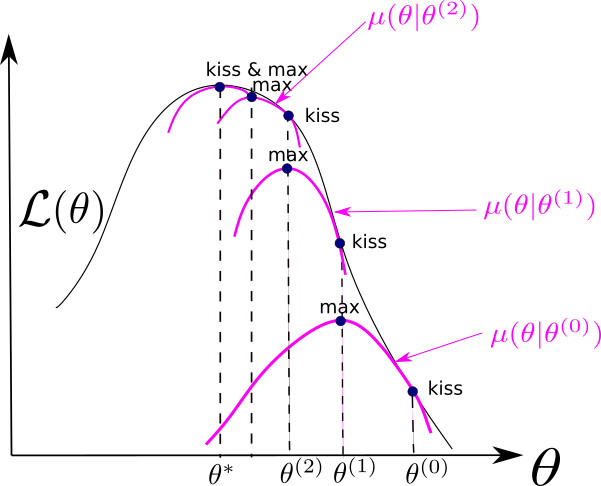
\includegraphics[width=3.7in]
{emax/minorize.png}
\caption{Function $\mu(\theta|\theta^{(t)})$
minorizes the function $\call(\theta)$.
Note that $\mu(\theta|\theta^{(t)})$
is always below
 $\call(\theta)$.
``max" indicates 
$\theta^{(t+1)}=
\argmax_\theta \mu(\theta|\theta^{(t)})$.
``kiss" indicates
 $\mu(\theta^{(t)}|\theta^{(t)})=
\call(\theta^{(t)})$. 
}
\label{fig-minorize}
\end{figure}



A function {\bf $\mu(\theta|\theta^{(t)})$ 
is said to minorize 
 a target
 function $\call(\theta)$}
iff for all $ \theta$ at fixed 
$\theta^{(t)}$,
it satisfies the
``$\mu\leq\call$ property"


\beq
\mu(\theta|\theta^{(t)})\leq
\call(\theta)
\;,
\eeq
and
the ``$\mu=\call$ property"

\beq
\mu(\theta^{(t)}|\theta^{(t)})=
\call(\theta^{(t)})
\;.
\eeq

We  {\bf recursively maximize a minorizing function} $\mu(\theta|\theta^{(t)})$
if we define a sequence $(\theta^{(t)})_{t=0, 1, \ldots}$
as follows:

\beq
\theta^{(t+1)}=\argmax_\theta \mu(\theta|\theta^{(t)})
\;.
\eeq

The sequence 
$(\call(\theta^{(t)}))_{t=0, 1, 2, \ldots}$
generated by 
recursively maximizing a minorizing function
must be nondecreasing:

\beq
\call(\theta^{(t+1)})\geq \mu(\theta^{(t+1)}
|\theta^{(t)})\geq
 \mu(\theta^{(t)}|\theta^{(t)}) 
= \call(\theta^{(t)})
\;.
\eeq

A {\bf
minorize-maximize (MM) algorithm}
is any algo that
specifies a
minorizing function $\mu(\theta|\theta^{(t)})$
for a particular target
 function $\call(\theta)$.
One can also define a 
{\bf majorize-minimize algo (also
called  MM)}
by inverting the inequalities throughout.


The EM algo is an MM algo.
Indeed, if we define 

\beq
\call(\theta)=\ln P(\vecx|\theta)
\eeq
and

\beq
\mu(\theta|\theta^{(t)})
=
Q(\theta|\theta^{(t)})
+
H(P(\ul{\vech}|\vecx, \theta^{(t)})
\;,
\eeq
then Eq.(\ref{eq-Q-decomposed})
establishes
the $\mu\leq \call$
and $\mu=\call$ properties
required of 
a minorizing function.

How an MM algo works 
is portrayed in Fig.\ref{fig-minorize}.


\section{Examples}

\subsection{Gaussian mixture}


$x[\sigma]\in \RR^d=S_\rvx$. $S_\rvh$ discrete and
not too large. $n_\rvh=|S_\rvh|$ is
number of Gaussians that we are 
going to fit the samples with.

Let
\beq
\theta = [w_h, \mu_h, \Sigma_h]_{h\in S_\rvh}
\;,
\eeq
where
$[w_h]_{h\in S_\rvh}$ is a probability
distribution of weights, and 
where $\mu_h\in\RR^d$
and $\Sigma_h\in\RR^{d\times d}$
are the mean value vector 
and covariance matrix of
a $d$-dimensional Gaussian distribution.

The TPMs, printed in blue,
for the nodes of Fig.\ref{fig-em-bnet},
for the special case
of a mixture of Gaussians, are as follows:

\beq\color{blue}
P(x[\sigma]\cond h[\sigma]\cond \theta)=
\caln_d(x[\sigma];\mu_{h[\sigma]}, \Sigma_{h[\sigma]})
\eeq

\beq\color{blue}
P(h[\sigma]\cond \theta)=w_{h[\sigma]}
\eeq

Note that

\beqa
P(x[\sigma]\cond \theta)&=&
\sum_h P(x[\sigma]\cond h[\sigma]=h, \theta)
P(h[\sigma]=h\cond\theta)
\\
&=&
\sum_hw_h\caln_d(x[\sigma];\mu_h, \Sigma_h)
\eeqa

\beqa
P(\vecx, \vech|\theta)&=&
\prod_\sigma \left[
w_{h[\sigma]}
\caln_d(x[\sigma];\mu_{h[\sigma]}, \Sigma_{h[\sigma]})
\right]
\\
&=&
\prod_\sigma\prod_h
\left[w_h
\caln_d(x[\sigma];\mu_h, \Sigma_h)\right]
^{\indi(h=h[\sigma])}
\eeqa

{\bf Old Faithful:}
See Wikipedia Ref.\cite{wiki-em}
for an animated
gif of a  classic example
of using EM to fit
samples with a Gaussian mixture.
Unfortunately,
could
not include it
here because pdflatex
does not support animated gifs. 
The gif shows samples in a 2 dimensional
space
(eruption time, delay time)
from the Old Faithful geyser.
In that example, $d=2$ and $n_\rvh=2$.
Two clusters of points
in a plane are fitted
by 
a mixture of 2 Gaussians.

{\bf K-means clustering} is often
presented as the main competitor
to EM for doing 
{\bf clustering (non-supervised
learning)}. In K-means clustering,
the sample points are 
split into $K$
mutually
disjoint sets $S_0, S_1, \ldots, S_{K-1}$. 
The algorithm is easy
to describe:
\begin{enumerate}
\item
Initialize by 
choosing  at random
$K$ data points $(\mu_k)_{k=0}^{K-1}$
called means or centroids
and placing $\mu_k$ in $S_k$
for all $k$.
 \item {\bf STEP 1:}
For each data point,
add it to the $S_k$
whose centroid $\mu_k$
is closest to it.
\item {\bf STEP 2:}
Recalculate the centroids.
Set $\mu_k$ equal to the mean value of set
$S_k$.
\item Repeat steps 1 and 2 until the
centroids stop changing 
by much.
\end{enumerate}
Step 1 is analogous
to the expectation step in EM,
and Step 2 to the maximization
step in EM ($\theta$
estimation versus 
$\mu_k$ estimation).
We won't say anything further
about K-means clustering because
it
isn't related to bnets in any 
way, and this is a book about bnets.
For more info about
K-means clustering, 
see Ref.\cite{wiki-k-means}.

\subsection{
Blood Genotypes and Phenotypes}

Notation:
$\vec{\rva}=
(\rva[\sigma])_{\sigma=0, 1, \ldots,nsam-1}
$, where $nsam$
is the number of samples.
Will
sometimes
denote
$a\sqsig$ by $a^\sqsig$.


Suppose
$\vec{\rvx}=
(\vec{\rvx}_0)
$ (i.e., just one component)

$\vec{\rvh}=
(\vec{\rvh}_0)
$ (i.e., just one component)



$\rvh[\sigma]\in S_\rvh=
\{AA, AO, BB, BO, OO, AB\}$ (the 6 blood genotypes)

$\rvx[\sigma]\in S_\rvx=
\{A,B,O,AB\}$ (the 4 blood phenotypes)

\begin{figure}[h!]
$$
\xymatrix{
\ul{\theta}\ar[d]\ar[dr]
\\
\rvx[\sigma]&\rvh[\sigma]\ar[l]
}$$
\caption{bnet 
for blood phenotypes $x\sqsig$
and genotypes $h\sqsig$.}
\label{fig-phenotypes}
\end{figure}

For the bnet of Fig.\ref{fig-phenotypes},
the TPMs, printed in blue, are:
\beq\color{blue}
P(h^\sqsig| \theta)=
\begin{array}{c|c}
&
\\\hline
AA&p_A^2
\\
AO&2p_Ap_O
\\
BB&p_B^2
\\
BO&2p_Bp_O
\\
OO&p_O^2
\\
AB&2p_Ap_B
\end{array}
\;,
\label{eq-pheno-ph}
\eeq
where $p_A+p_B+p_O=1$.


\beq\color{blue}
P(x^\sqsig\cond h^\sqsig, \theta)=
\begin{array}{l|llllll}
&AA&AO&BB&BO&OO&AB
\\\hline
A&1&1&0&0&0&0
\\
B&0&0&1&1&0&0
\\
O&0&0&0&0&1&0
\\
AB&0&0&0&0&0&1
\end{array}
\label{eq-pheno-pxbarh}
\eeq

\beq
\theta=(p_A, p_B)
\eeq

Multiplying the TPMs in
Eqs.(\ref{eq-pheno-ph}
and (\ref{eq-pheno-pxbarh}), we get
\beq
P(x^\sqsig\cond \theta)=
\begin{array}{l|l}
\\\hline
A&p_A^2+2p_Ap_O(=\pi_A)
\\
B&p_B^2+2p_Bp_O(=\pi_B)
\\
O&p_O^2(=\pi_O)
\\
AB&2p_Ap_B(=\pi_{AB})
\end{array}
\eeq


Note that 
\beqa
P(\vec{x}|\theta)
&=&
\prod_\sigma
P(x^\sqsig|\theta)
\\
&=&
(\pi_A)^{N_A}
(\pi_B)^{N_B}
(\pi_O)^{N_O}
(\pi_{AB})^{N_{AB}}
\;,
\eeqa 
where 
$N_x$ for $x\in S_\rvx=\{A, B, O, AB\}$
are
the counts from the data.
We can get estimates
for the parameters $p_A$ and $p_B$
right
here without doing EM.
Just note that

\beq
\hat{\pi}_x=
\frac{N_x}
{N_+}
\label{eq-quads-pi-x}
\eeq
for $x\in S_\rvx$,
where
$N_+=\sum_x N_x$. 
Eqs.(\ref{eq-quads-pi-x})
give  4 quadratic equations
that can be solved for the
parameters $p_A, p_B$
in terms of the observed 
counts $N_x$
for $x\in S_\rvx$.


If, instead,  you want to
find the optimum
parameters $p_A, p_B$
using EM, note that

\beqa
Q(\theta|\theta^{(t)})
&=&
\sum_{\vec{h}}
P(\vec{h}|\theta^{(t)})
\ln P(\vec{x}, \vec{h}|\theta)
\\
&=&
\sum_{\vec{h}}
\left[\prod_\sigma
P(h^\sqsig|\theta^{(t)})
\right]
\ln \left[
\prod_\sigma P(x^\sqsig, h^\sqsig |\theta)
\right]
\\
&=&\sum_\sigma 
\sum_{h^\sqsig}
P(h^\sqsig|\theta^{(t)})
\ln
 P(x^\sqsig, h^\sqsig |\theta)
\\
&=&\sum_\sigma 
\sum_{h^\sqsig}
P(h^\sqsig|\theta^{(t)})
[\ln
 P(x^\sqsig| h^\sqsig ,\theta)
+
\ln
 P(h^\sqsig |\theta)
]
\\
&=&nsam 
\sum_{h^\sqsig}
P(h^\sqsig|\theta^{(t)})
\ln
 P(h^\sqsig |\theta)
\;.
\eeqa

\subsection{Missing
 Data/Imputation}

The previous example
on blood genotypes and phenotypes
assumed no missing
data in compiling the
counts $N_x$. 
But what if there is missing
data? Can one
still apply
the EM algo in that case?
Yes! See Chapter \ref{ch-missing-d}.



\chapter{Frisch-Waugh-Lovell (FWL) theorem}

The Frisch-Waugh-Lovell (FWL) theorem
(see Ref.\cite{wiki-fwl-theo})
(mnemonic: FoWL Theorem)
is a method used in Linear Regression (LR).
It allows us to
calculate
a regression coefficient
by doing LR on residuals
calculated from two previously
performed LRs.

As in the section \nameref{sec-conv-lr}
on LR, we will consider
two cases: $x^\s$ non-random, and $x^\s$ random i.i.d.).

\section{FWL, assuming $x^\s$ are nonrandom}
Suppose
\beq
y=  X_1\beta_1 + X_2\beta_2 + \eps
\label{eq-y-x1-x2-eps}
\eeq
where

$y, \eps\in \RR^{nsam}$

$X_a\in \RR^{nsam\times k_a}$,
$\beta_a\in \RR^{k_a}$ for $a=1,2$

Define the matrices $U_1$ and $A_1$ by

\beq
U_1 = X_1(X_1^TX_1)^{-1}X_1^T
\eeq
and

\beq
A_1 = 1-U_1
\;.
\eeq
Note that

\beq
U_1X_1=X_1\;,\;\;A_1X_1=0
\eeq
(mnemonic: $A_1$ Annihilates $X_1$,
and $U_1$ acts like Unity on $X_1$).

Applying $A_1$ to Eq.(\ref{eq-y-x1-x2-eps}) gives

\beq
A_1 y = A_1X_2\beta_2  + A_1\eps
\eeq
so we can estimate $\beta_2$ by

\beq
\boxed{
\hat{\beta}_2=
(A_1X_2)^{-1}A_1 y}
\label{eq-fwl-nonrand}
\;.
\eeq
\section{FWL, assuming $x^\s$ are random}


Assume for simplicity that 
$k_1=k_2=1$
in Eq.(\ref{eq-y-x1-x2-eps}). Let
$\beta_1=\alp\in\RR$, 
$\beta_2=\beta\in\RR$.
When the $x^\s$ are random and i.i.d.,
and
$X_1, X_2$ are
replaced by 
the random variables
$\rvx, \rvd\in \RR$,
Eq.(\ref{eq-y-x1-x2-eps})
is equivalent to


\beq
\rvy=\alpha \rvx + \beta \rvd
+ \rvu_\rvy
\label{eq-y-ax-bd-u}
\;.
\eeq

As usual, we will denote
the linear operator
$\av{\rvx,\rvx}^{-1}\av{\rvx, \cdot}$
by a derivative operator:

\beq
\frac{\av{\rvx, \cdot}}
{\av{\rvx,\rvx}}=
\frac{d\cdot}{d\rvx}
\;.
\eeq
Define operators $U_\rvx$ and $A_\rvx$ by

\beq
U_\rvx(\cdot)= \rvx\frac{d\cdot}{d\rvx}
\eeq
and

\beq
A_\rvx = 1 - U_\rvx
\;.
\eeq
Note that

\beq
U_\rvx\rvx=\rvx\;,\;\;
A_\rvx \rvx=0
\;.
\eeq

If we apply $A_\rvx$ to Eq.(\ref{eq-y-ax-bd-u}), we get

\beq
A_\rvx\rvy = \beta A_\rvx \rvd
+A_\rvx\rvu_\rvy
\;.
\eeq
Hence,

\beq
\av{A_\rvx\rvd, A_\rvx\rvy}=
\beta\av{A_\rvx\rvd, A_\rvx\rvd}
\;.
\eeq
Thus,

\beq
\boxed{
\beta = \frac{d (A_\rvx \rvy)}{dA_\rvx\rvd}
}
\;.
\label{eq-fwl-rand}
\eeq
\hrule
Eqs.(\ref{eq-fwl-nonrand})
and (\ref{eq-fwl-rand})
constitute our statement
of the FWL theorem. They
are the main result of this chapter.
But before ending this chapter,
let us show how the
FWL theorem for random $x^\s$
can be interpreted
graphical using LDEN diagrams
(LDEN diagrams
are discussed in Chapter \ref{ch-linear-sys}).


\begin{figure}[h!]
$$
\xymatrix{
&\rvx\ar[dr]^\alpha&\rvu_\rvy\ar[d]
\\
\rvd\ar[rr]_\beta&&\rvy
\\
&(a)
}\;\;\;
\xymatrix{\rvu_\rvd\ar[d]
&\rvx\ar[dr]^{\alpha'}\ar[dl]_\gamma
&\rvu'_\rvy\ar[d]
\\
\rvd&&\rvy
\\
&(b)}
\;\;\;
\xymatrix{
\\
A_\rvx\rvd\ar[rr]_\beta&&A_\rvx\rvy
\\
&(c)
}$$
\caption{LDEN diagrams for discussing the FWL theorem.
}
\label{fig-fwl-abc}
\end{figure}

Fig.\ref{fig-fwl-abc}$(a)$
is a graphical
representation of the following equation:
\begin{subequations}
\beq
\rvy = \alpha \rvx + \beta\rvd + \rvu_\rvy
\;.
\label{eq-fwl-a}
\eeq
Likewise, \ref{fig-fwl-abc}$(b)$
represents

\beq
\left\{
\begin{array}{l}
\rvd = \gamma \rvx + \rvu_\rvd
\\
\rvy = \alpha'\rvx + \rvu'_\rvy
\end{array}
\right.
\label{eq-fwl-b}
\eeq
and \ref{fig-fwl-abc}$(c)$
represents

\beq
A_\rvx\rvy = \beta A_\rvx \rvd
\;.
\label{eq-fwl-c}
\eeq
\end{subequations}

Applying $d/d\rvx$ to Eq.(\ref{eq-fwl-a}
yields

\beq
\frac{d\rvy}{d\rvx}=
\alp
+\beta\frac{d\rvd}{d\rvx}
\;.
\eeq
Applying $d/d\rvx$ to Eq.(\ref{eq-fwl-b}
yields


\beq
\gamma=\frac{d\rvd}{d\rvx}
\;,\;\;
\alp'=\frac{d\rvy}{d\rvx}
\;.
\eeq
Therefore,

\beq
\alp'=\alp +\beta\gamma
\;.
\eeq

Applying $A_\rvx$ to Eq.(\ref{eq-fwl-b})
yields
\beq
A_\rvx\rvy=(1-\rvx\frac{d}{d\rvx})\rvy=
\rvy-\alp'\rvx
\eeq
and

\beq
A_\rvx\rvd=
(1-\rvx\frac{d}{d\rvx})\rvd
=
\rvd-\gamma\rvx
\;.
\eeq
Therefore, Eq.(\ref{eq-fwl-c})
is equivalent to

\beq
\rvy-\alpha'\rvx = \beta(\rvd-\gamma\rvx)
\;.
\eeq
\chapter{Frontdoor Adjustment Formula}
\label{ch-fdoor}
The frontdoor (FD) adjustment
formula is proven in
Chapter \ref{ch-do-calc}
from the rules of Do Calculus.
The goal 
of this chapter is
to give examples
of the use of that
theorem. We will restate
the theorem in this chapter,
sans proof.
There is no need
to understand the
theorem's
proof in order to use it.
However, you
will
need to skim Chapter \ref{ch-do-calc}
in order to familiarize 
yourself with
the notation used to state the 
theorem.
This chapter also assumes
that you are comfortable 
with the  rules 
for checking for d-separation. Those rules
are covered in Chapter \ref{ch-dsep}.


\fdoordef

\begin{claim} Frontdoor Adjustment Formula

\fdoorclaim

\end{claim}
\proof 
See Chapter \ref{ch-do-calc}.
\qed

\section{Examples}

\begin{enumerate}
\item
\beq
\xymatrix{
&*++[F-o]{\rvc}\ar[ld]\ar[rd]
\\
\rvx\ar[r]&\rvm\ar[r]&\rvy
}
\eeq
Can't satisfy backdoor
criterion because $\rvc$
unobserved so
can't condition on it 
to block
backdoor path $\rvx-\rvc-\rvy$.

If $\rvx.=\rvx,\rvm.=\rvm$ 
and $\rvy.=\rvy$,
then the FD criterion
is satisfied. In fact,

\beq
\xymatrix{\\
P(y|\cald \rvx=x)=
}
\xymatrix{
&\EE x'\ar[rd]
\\
x\ar[r]&\sum m\ar[r]&y
}
\eeq


\hrule\item
\beq
\xymatrix{
*++[F-o]{\rvz_1}\ar[d]\ar[dr]
&&
*++[F-o]{\rvz_2}\ar[d]\ar[dl]
\\
*++[F-o]{\rvw_1}\ar[d]
&\rvc\ar[ld]\ar[rd]
&*++[F-o]{\rvw_2}\ar[d]
\\
\rvx\ar[r]&\rvm\ar[r]&\rvy
}
\eeq
Can't satisfy backdoor
criterion because 
to block 
backdoor path $\rvx-\rvc-\rvy$,
need to condition on $\rvc$
but if this is true, 
then long
path 
$\rvx-\rvw_1-\rvz_1-\rvc-\rvz_2-\rvw_2-\rvy$
becomes unblocked.

If $\rvx.=\rvx,\rvm.=\rvm$ 
and $\rvy.=\rvy$,
then the FD criterion
is satisfied. In fact,

\beqa
\xymatrix{\\
P(y|\cald\rvx=x)=
}
&&
\xymatrix{
*++[F-o]{\EE z_1}\ar[d]\ar[dr]
&&
*++[F-o]{\EE z_2}\ar[d]\ar[dl]
\\
*++[F-o]{\sum w_1}
&\sum c\ar[rd]
&*++[F-o]{\sum w_2}\ar[d]
\\
x\ar[r]&\sum m\ar[r]&y
}
\\
&=&
\xymatrix{
*++[F-o]{\EE x'}\ar[d]\ar[dr]
&&
*++[F-o]{\EE x''}\ar[d]\ar[dl]
\\
*++[F-o]{\sum w_1}
&\sum c\ar[rd]
&*++[F-o]{\sum w_2}\ar[d]
\\
x\ar[r]&\sum m\ar[r]&y
}
\\
&=&
\xymatrix{
&\EE x'\ar[rd]
&
\\
x\ar[r]&\sum m\ar[r]&y
}
\eeqa


\end{enumerate}
\chapter{G-formula (Sequential Backdoor
Adjustment Formula)}
\label{ch-g-formula}

\begin{figure}[h!]
\centering
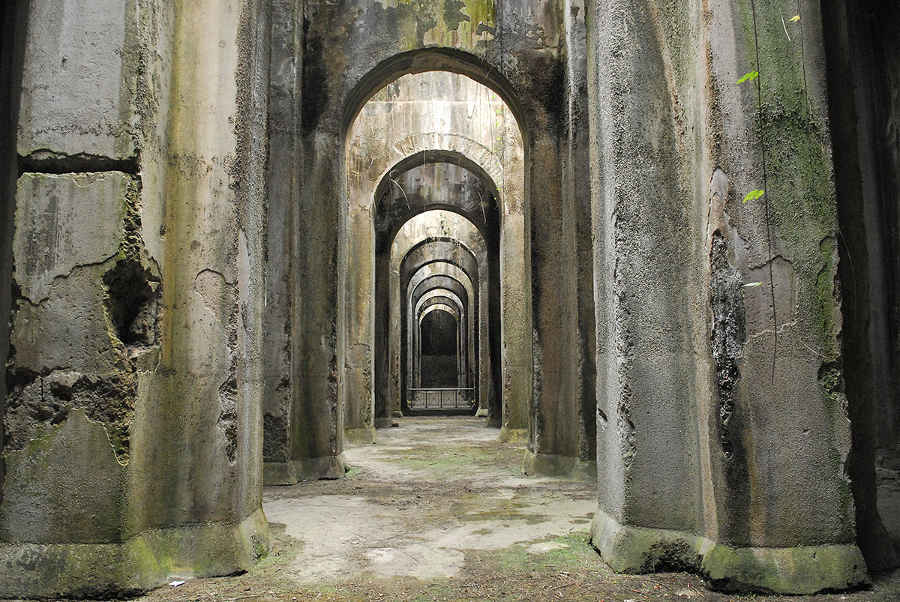
\includegraphics[width=5in]
{g-formula/piscina-mirabilis.jpeg}
\caption{Piscina Mirabilis,
ancient Roman cistern in Naples}
\label{fig-piscina}
\end{figure}


This chapter is based
on Ref.\cite{pearl-robins-95}
by Pearl and Robins.

A {\bf g-formula}\footnote{It's
not clear from the literature what the \qt{g}
stands for. I assume it stands for \qt{generating}.
}
is any formula that
defines recursively the full
probability distribution of a bnet.
In other words, it's a recursive
definition of a Dynamical Bayesian Network.\footnote{Dynamical
Bayesian Networks
are discussed in Chapter \ref{ch-dyn-bnets}.}


The goal of this
chapter is to
generalize
the backdoor adjustment
formula (see Chapter \ref{ch-bdoor})
from
a query $P(y|\cald\rvx=x)$
with a single
do node to a query
$P(y|\cald\rvx^n=x^n)$
with multiple
do nodes.
The resulting generalized adjustment
formula is called  a {\bf sequential backdoor (SBD)
adjustment formula},
and it is associated with
an {\bf
SBD  g-formula}.

For $n=1,2,3 \ldots$, define
\beqa
\calq(y|x^n)&=&
\sum_{z^n}
P(y|x^n, z^n)
\prod_{t=0}^{n-1}
P(z_t|x_{<t}, z_{<t})
\\
&&
\xymatrix{
&\sum_{z^n}
\\
=
}
\xymatrix{
z^n\ar[d]
\\
y
\\
x^n\ar[u]
}
\xymatrix{\\
\prod_{t=0}^{n-1}}
\xymatrix{
z_{<t}\ar[r]
&z_t
\\
\\
x_{<t}\ar[uur]
}
\label{def-q-y-xn-seqbdoor}
\eeqa

For $n=1$,
\beq
\xymatrix{\\
\calq(y|x_0)
}
\xymatrix{
&\sum_{z_0}
\\
=
}
\xymatrix{
z_0\ar[d]
\\
y
\\
x_0\ar[u]
}
\xymatrix{P(z_0)\\ \\}
\xymatrix{
\\
=\quad
}
\xymatrix{
\EE z_0\ar[dr]
\\
& y
\\
x_0\ar[ur]
}
\;.
\eeq

For $n=2$,

\begin{align}
\xymatrix{
\\
\calq(y|x^2)
}
&
\xymatrix{
&\sum_{z^2}
\\
=
}
\xymatrix{
(z_0,z_1)\ar[d]
\\
y
\\
(x_0,x_1)\ar[u]
}
\xymatrix{
P(z_0)
}
\xymatrix{
z_0\ar[r]
&z_1
\\
\\
x_0\ar[ruu]
}
\\
&
\xymatrix{\\=}
\xymatrix{
\EE z_0\ar[r]\ar[drr]
&\sum z_1\ar[dr]
\\
&&y
\\
x_0\ar[ruu]\ar[urr]
&x_1\ar[ur]
}
\;.
\end{align}

For $n=3$,

\begin{align}
\xymatrix{\\
\calq(y|x^3)
}
&
\xymatrix{
&\sum_{z^3}
\\
=
}
\xymatrix{
(z_0,z_1,z_2)\ar[d]
\\
y
\\
(x_0,x_1, x_2)\ar[u]
}
\xymatrix{
P(z_0)
}
\xymatrix{
z_0\ar[r]
&z_1
\\
\\
x_0\ar[ruu]
}
\xymatrix{
(z_0,z_1)\ar[r]
&z_2
\\
\\
(x_0,x_1)\ar[ruu]
}
\\
\nonumber
\\
&
\xymatrix{
&\sum_{z^3}
\\
=
}
\xymatrix{
(z_0,z_1,z_2)\ar[d]
\\
y
\\
(x_0,x_1, x_2)\ar[u]
}
\xymatrix{
P(z_0)
}
\xymatrix{
z_0\ar[r]\ar@/^1pc/[rr]
&z_1\ar[r]
&z_2
\\
\\
x_0\ar[uur]\ar[uurr]
&x_1\ar[uur]
&x_2
}
\\
\nonumber
\\
&
\xymatrix{\\=}
\xymatrix{
\EE z_0\ar[r]\ar@/^1pc/[rr]
\ar[drrr]
&\sum z_1\ar[r]
\ar[drr]
&\sum z_2
\ar[dr]
\\
&&&y
\\
x_0\ar[uur]\ar[uurr]
\ar[urrr]
&x_1\ar[uur]
\ar[urr]
&x_2
\ar[ur]
}
\end{align}



\SeqBdoorDef

\begin{claim}(SBD Adjustment Formula)

\SeqBdoorClaim
\end{claim}
\proof
If
$z^n$
satisfies the SBD
criterion
relative
to
$(\rvx^n, \rvy)$,
then
$\rvx^n, \rvy, \rvz^n$
might
have the following
structure for $n=3$.

\beq
\xymatrix{
\rvz_0\ar[r]\ar@/^1pc/[rr]\ar[drrr]
\ar[dd]
&\rvz_1\ar[r]\ar[drr]
\ar[dd]
&\rvz_2\ar[dr]
\ar[dd]
\\
&&&\rvy
\\
\rvx_0\ar[uur]\ar[uurr]\ar[urrr]
\ar[r]\ar@/_1pc/[rr]
&\rvx_1\ar[uur]
\ar[urr]\ar[r]
&\rvx_2
\ar[ur]
}
\label{eq-seq-bdoor-special}
\eeq

One can check
using the following 3
auxiliary bnets
that bnet Eq.(\ref{eq-seq-bdoor-special})
satisfies the
SBD
criterion.
Note that conditioned
nodes are shaded yellow.
\beq
\begin{array}{ccc}
\xymatrix@C=.95pc{
*++[o][F*:yellow]{\rvz_0}\ar[r]\ar@/^1pc/[rr]\ar[drrr]
\ar[dd]
&*++[o][F*:yellow]{\rvz_1}\ar[r]\ar[drr]
&*++[o][F*:yellow]{\rvz_2}\ar[dr]
\\
&&&\rvy
\\
\rvx_0
&\rvx_1\ar[uur]
\ar[urr]
&\rvx_2
\ar[ur]
}
&
\xymatrix@C=.95pc{
\rvz_0\ar[r]\ar@/^1pc/[rr]\ar[drrr]
\ar[dd]
&*++[o][F*:yellow]{\rvz_1}\ar[r]\ar[drr]
\ar[dd]
&*++[o][F*:yellow]{\rvz_2}\ar[dr]
\\
&&&\rvy
\\
*++[o][F*:yellow]{\rvx_0}
\ar[uur]\ar[uurr]\ar[urrr]\ar[r]
&\rvx_1
&\rvx_2
\ar[ur]
}
&
\xymatrix@C=.95pc{
\rvz_0\ar[r]\ar@/^1pc/[rr]\ar[drrr]
\ar[dd]
&\rvz_1\ar[r]\ar[drr]
\ar[dd]
&*++[o][F*:yellow]{\rvz_2}\ar[dr]
\ar[dd]
\\
&&&\rvy
\\
*++[o][F*:yellow]{\rvx_0}
\ar[uur]\ar[uurr]\ar[urrr]
\ar[r]\ar@/_1pc/[rr]
&*++[o][F*:yellow]{\rvx_1}\ar[uur]
\ar[urr]\ar[r]
&\rvx_2
}
\\
\\
\call_{\rvx_0}\cald_{\rvx_1, \rvx_2}G
&\call_{\rvx_1}\cald_{\rvx_2}G
&\call_{\rvx_2}G
\end{array}
\eeq



See Claim \ref{cl-decSeqBackDoor}
for a proof of this claim
for the special case
Eq.(\ref{eq-seq-bdoor-special}).
\qed

\chapter{Gaussian Nodes with
 Linear Dependence on Parents}
\label{ch-gauss-lin}

Bnet nodes
that 
have a Gaussian TPM
with a linear dependence
on their parent nodes (GLP)
are a very
popular way 
of modeling continuous
nodes of bnets.
A 
convenient
aspect of them
is that their
parents can be discrete
or continuous nodes,
and their
children can be discrete
or continuous nodes too.
Also,
they can be learned 
easily
from the data
because
their
parameters
can
be expressed in terms of
two node
covariances.
For these reasons, 
they are commonly
used when 
doing
structure learning of 
bnets 
with continuous nodes (see Chapter \ref{ch-struc-learn}).

\begin{figure}[h!]
$$\xymatrix{
\rvy
&\rvx_1\ar[l]
\\
&\rvx_2\ar[lu]
\\
&\rvx_3\ar[luu]
}$$
\caption{GLP node
$\rvy$ with 3 parent nodes $\rvx^3
=
(\rvx_1, \rvx_2, \rvx_3)$.}
\label{fig-glp-3}
\end{figure}

Recall our
notation
for a Gaussian distribution:
\beq
\caln(x;\mu, \sigma^2)
=
\frac{1}{\sigma\sqrt{2\pi}}
e^{\frac{-(x-\mu)^2}{2\sigma^2}}
\;,
\eeq
where 
$x, \mu\in \RR$
and $\sigma>0$.

A GLP node $\rvy$ with 
$n$ parents
 $\rvx^n=(\rvx_1, \rvx_2, \ldots, \rvx_n)$
has the following TPM:
\beq\color{blue}
P(y|x^n)=
\caln(y; \beta_0 + 
\beta^{nT}x^n, \sigma^2)
\eeq
where $\rvy, \beta_0, \in\RR$
and $\sigma^2>0$, and where
$\rvx^n, \beta^n\in \RR^n$ 
are **column vectors**.
The $T$ 
in $\beta^{nT}$ stands for transpose.
Any $\rvx_i$
can have
a discrete
set of states
as long as they are real
valued and ordinal (ordered by size).
 Fig.\ref{fig-glp-3}
shows a diagrammatic
representation
of a GLP node with 3 parents.

Note that as $\sigma\rarrow 0$,
a GLP node becomes 
deterministic.
In fact,
it
becomes a neural
net node
with a linear activation function.


An equivalent
way of defining a GLP node $\rvy$
is in terms of a random variable
equation expressing
$\rvy$ as a hyperplane
function of the parents $\rvx^n$
plus a  Gaussian noise variable.
Define a curve-fit $\HAT{\rvy}$
of a \qt{true value}
$\rvy$ by
\begin{subequations}
\beq
\HAT{\rvy}=\beta_0 + \beta^{nT}\rvx^n
\eeq
and

\beq
\rvy=\HAT{\rvy}+\ul{\eps}
\eeq
where the residual $\ul{\eps}$
satisfies 

\beq
P(\eps)=\caln(\eps; 0, \sigma^2)
\eeq
and


\beq
\av{\rvx^n, \ul{\eps}}
=0
\;.
\eeq
\end{subequations}

The notation $\av{\rvx, \rvy}$
for the covariance
of random variables
$\rvx$ and $\rvy$
is explained
in Chapter \ref{ch-conventions}.

\begin{claim}
The
parameters of
a GLP node
can be expressed
in terms of 2-node
covariances.
Specifically,

\beq
\beta^n=
\av{\rvx^n, \rvx^{nT}}^{-1}
\av{\rvy, \rvx^n}
\eeq

\beq
\beta_0=
\av{\rvy}-
\beta^{nT}\av{\rvx^n}
\eeq

\beq
\sigma^2
=
\av{\rvy, \rvy}
-\beta^{nT}
\av{\rvx^n, \rvy}
\eeq
\end{claim}
\proof

Note that $\av{\rvx^n, \rvx^{nT}}^T
=\av{\rvx^n, \rvx^{nT}}$
and 
$\av{\rvy, \rvx^{nT}}^T
=\av{\rvy, \rvx^n}$.


\beq
\av{\rvy, \rvx^{nT}}
=
\beta^{nT}\av{\rvx^n, \rvx^{nT}}
\eeq

\beq
\av{\rvy, \rvx^n}=
\av{\rvx^n, \rvx^{nT}}\beta^n
\eeq

\beq
\beta^n
=
\av{\rvx^n, \rvx^{nT}}^{-1}
\av{\rvy, \rvx^n}
\eeq

\beq
\av{\rvy}=
\beta_0 + 
\beta^{nT}\av{\rvx^n}
\eeq

\beqa
\av{\rvy, \rvy}
&=&
\av{
\beta_0 + \beta^{nT}\rvx^n +
\ul{\eps},
\rvy}
\\
&=&
\beta^{nT}\av{\rvx^n,
\rvy}
+
\sigma^2
\eeqa
\qed

\hrule
Let  D=Discrete, GLP=Gaussian with  Linear
 dependence in Parents

The following arrows are possible
in a bnet.

\begin{itemize}
\item $GLP\larrow GLP$
\item $GLP\larrow D$

Pass to GLP a separate
set of regression
coefficients $\beta_0, \beta^n$
and variance $\sigma^2$
for each state 
of D. If D is called $\rvd$,
let
\beq\color{blue}
P(y|(x^n)_d, d)=
\caln(y; (\beta_0)_d + 
(\beta^{nT})_d (x^n)_d, \sigma_d^2)
\eeq
for each $d\in S_{\rvd}$.

\item $D\larrow GLP$

If D expects
a continuous parent,
no need to preprocess GLP output.
If D expects a discrete parent,
break
the interval $[a,b]$
that
contains
most of
the range
of the GLP node into
sub-intervals and 
assign a discrete label
to each subinterval.
\item $D\larrow D$
\end{itemize}
\chapter{Generalized Linear Model (GLM)}
\label{ch-gen-lin-mod}

This chapter is based on
chapter 4 of Ref.\cite{agresti-book}.

\section{Exponential Family of Distributions}
\label{sec-exp-fam}

The {\bf Exponential Family (EF)} of probability distributions is defined by

\beq
P(y|\theta, \phi) =
\exp\left(\frac{\theta y - b(\theta)}{a(\phi)}+c(y,\phi)\right)
\eeq

In this chapter, we will
denote averages over $y|\theta, \phi$ by angular brackets

\beq
E_{\rvy|\theta, \phi}[f(y)] = \sum_y P(y|\theta, \phi) f(y) = \av{f(y)}
\eeq
As usual in this book, let $S_\rvx$ denote the set of
values that the random variable $\rvx$ can take.
We will assume that $S_\rvy$
for EF
can be either a discrete or a continuous
subset of $\RR$,\footnote{By a \enquote{continuous set} we
mean a finite set of intervals
 each of which has non-zero length.}
but $S_{\ul{\theta}}$
must be continuous.
When $S_\rvy$ is a discrete subset of $\RR$, $P(y|\theta, \phi)$
will denote a probability distribution, whereas when
$S_\rvy$ is continuous, it will denote
a probability density.

\begin{claim}
\beq
\mu = \av{\rvy} = b'(\theta)
\eeq

\beq
\s^2= \av{\rvy, \rvy} = a(\phi)b''(\theta)
\eeq
\end{claim}
\proof

\beqa
0&=& \partial_\theta \int_{-\infty}^\infty
dy\; P(y|\theta, \phi)
\\
&=&
\int_{-\infty}^\infty
dy\;\frac{1}{a}
[y-b'(\theta)]P(y|\theta, \phi)
\\
&=&
\frac{1}{a}[\av{\rvy}-b'(\theta)]
\eeqa

\beqa
0&=& \partial^2_\theta \int_{-\infty}^\infty
dy\; P(y|\theta, \phi)
\\
&=&
\int_{-\infty}^\infty
dy\;\left\{\frac{-b''(\theta)}{a} +
\frac{1}{a^2}
[y-b'(\theta)]^2\right\}
P(y|\theta, \phi)
\eeqa
Hence,

\beq
\av{[y-b'(\theta)]^2}= a b''(\theta)
\eeq

\qed

Note that the Normal Distribution
belongs to the EF. Indeed,

\beqa
\caln(y; \mu, \s^2)
&=&
\frac{1}{\sqrt{2\pi \s^2}}
\exp\left(
-\;\frac{(y-\mu)^2}{2\s^2}
\right)
\\
&=&
\exp\left(
\frac{-y^2 + 2\mu y -\mu^2}{2\s^2}
-\ln\sqrt{2\pi \s^2}
\right)
\\
&=&
\exp\left(
\frac{-\;\frac{1}{2}y^2 + \mu y -\;\frac{1}{2}\mu^2}{\s^2}
-\ln\sqrt{2\pi \s^2}
\right)
\eeqa
So, for the
Normal Distribution, $\theta=\mu$ , $a=\s^2$, $b=\mu^2/2$,
$b'=\mu$, $b''=1$.

EF can be defined for an ensemble
 $\{y_\s:\s\in \Sigma\}$ of
 independent (but not
 necessarily identically
 distributed) random variables $y_\s$
 describing individuals $\s$
 of a population $\Sigma$.

\beq
P(\vecy|\vtheta, \phi) =
\prod_\s
\exp\left(\frac{\theta_\s y_\s - b(\theta_\s)}{a(\phi)}+c(y_\s ,\phi)\right)
\eeq

\beq
\mu_\s = \av{\rvy_\s}= \partial_{\theta_\s} b(\theta_\s)
\eeq

\beq
\av{\rvy_\s, \rvy_{\s'}} =
\delta(\s, \s')
a(\phi) \partial^2_{\theta_\s}b(\theta_\s)
\eeq

\section{GLM}
The Generalized Linear Model (GLM)
is a statistical model for an ensemble of independent
(but not necessarily identically
distributed) random variables $\rvy_\s$.
GML consists of
3 parts:

\begin{enumerate}
\item Exponential Family

Model $\rvy_\s$ by probability distribution
of exponential family (EF).

\item Linear predictor

In EF, replace $\theta_\s$ by
the {\bf linear predictor} $\xbeta= \sum_i X_{\s, i}\beta_i$.
$\xbeta$ is commonly denoted by $\eta_\s$,
but I will avoid that notation because
I think the results are much clearer
when expressed in the more explicit notation $\xbeta$ instead
of $\eta_\s$.

\item Link Function

\beq
\mu_\s = \av{\rvy_\s} = \partial_{\xbeta} b
\eeq

\beq
\xbeta = g(\mu_\s) = \HAT{\theta}(\mu_\s)
\eeq

\beq
\mu_\s = g^{-1}(\xbeta)=\HAT{\mu}(\xbeta)
\eeq


$\HAT{\theta}()=g()$ is called
the {\bf link function}.
\end{enumerate}


Note that in
Linear Regression (LR),
we consider
independent (but
not necessarily
identically distributed) random variables $\rvy_\s\in \RR$
that satisfy

\beq
\rvy_\s = \xbeta + \ul{\eps}_\s
\eeq
where

\beq
\av{\eps_\s}=0, \quad
\av{\ul{\eps}_\s, \ul{\eps}_\s} =\delta(\s, \s')\s^2_\s
\eeq
Equivalently, one states that
\beq
\rvy_\s \sim \caln(\mu_\s=\xbeta, \s^2_\s)
\eeq
Hence, for LR, the link function and its
inverse are the identity map.

For the Bernoulli distribution with $y_\s\in \bool$,
\beqa
Ber(y_\s;p_\s) &=& p_\s^{y_\s} (1-p_\s)^{1-y_\s}
\\
&=&
\exp(y_\s\ln p_\s + (1-y_\s)\ln(1-p_\s))
\\
&=&
\exp\left( y_\s
\underbrace{\ln\left(\frac{p_\s}{1-p_\s}\right)}_{\xbeta}
+\underbrace{\ln (1-p_\s)}_{-b}\right)
\eeqa


$\mu_\s = p_\s$,
and $\xbeta= \lodds(\mu_\s)$ so $\mu_\s= \smoid(\xbeta)$.

$g() =\lodds()$ and $g^{-1}() =\smoid()$

\beq
a=1
\eeq

\beqa
b
&=&
 -\ln (1-\mu_\s)
\\
&=&
-\ln\left(
1-\;\frac{1}{1+e^{-\xbeta}}
\right)
\\
&=&
-\ln\left(
\frac{e^{-\xbeta}}{1+e^{-\xbeta}}
\right)
\\
&=&
\ln(1+e^{\xbeta})
\eeqa

\beqa
\partial_{\xbeta} b &=&
\frac{e^{\xbeta}}{1+e^{\xbeta}}
\\
&=& \smoid(\xbeta)
\\
&=&\mu_\s
\eeqa

Table \ref{tab-ef-link-fun}
gives various probability distributions
and their natural link functions,
for cases where the link function is
simple and  easy to invert.

% Please add the following required packages to your document preamble:
% \usepackage[table,xcdraw]{xcolor}
% If you use beamer only pass "xcolor=table" option, i.e. \documentclass[xcolor=table]{beamer}
\begin{table}[h!]
\centering
\begin{tabular}{|
>{\columncolor[HTML]{FFFFC7}}l |l|l|}
\hline
\cellcolor[HTML]{F6F694}prob. distribution & \cellcolor[HTML]{F6F694}link function
$\xbeta=g(\mu_\s)$ & \cellcolor[HTML]{F6F694}$\mu_\s=g^{-1}(\xbeta)$ \\ \hline
\begin{tabular}[c]{@{}l@{}}Normal\\ $\rvy_\s\in(-\infty, +\infty)$\end{tabular} & \begin{tabular}[c]{@{}l@{}}$\xbeta= \mu_\s$\\ ($g$= identity map)\end{tabular} & $\mu_\s = \xbeta$ \\ \hline
\begin{tabular}[c]{@{}l@{}}Exponential\\ $\rvy_\s\in  (0, +\infty)$\end{tabular} & $\xbeta= -\;\frac{1}{\mu_\s}$ & $\mu _\s= -\;\frac{1}{\xbeta}$ \\ \hline
\begin{tabular}[c]{@{}l@{}}Poisson\\ $\rvy_\s\in \{0,1,2, \ldots\}$\end{tabular} & $\xbeta = \ln \mu_\s$ & $\mu_\s = \exp(\xbeta)$ \\ \hline
\begin{tabular}[c]{@{}l@{}}Bernoulli\\ $\rvy_\s\in\bool$\end{tabular} & $\xbeta = \lodds(\mu_\s)$ & $\mu_\s = \smoid(\xbeta)$ \\ \hline
\end{tabular}
\caption{Various probability distributions and their natural link functions.}
\label{tab-ef-link-fun}
\end{table}

 GLM is a generalization of LR. Recall
 some of the main results  of LR:
\beq
y = X\beta + \eps
\eeq

\beq
\av{\eps}=0, \quad
\av{\eps, \eps^T}= \s^2 I_N
\eeq
where $I_N$ is the
$N=|\Sigma|$ dimensional
unit matrix.

The Maximum Likelihood Estimate  (MLE)
for $\beta$ is

\beq
\HAT{\beta}=
(X^T X)^{-1} X^T y
\;.
\eeq
The covariance of $\HAT{\beta}$ is

\beqa
\av{\HAT{\beta},\HAT{\beta}^T}
&=&
\av{X^T X)^{-1} X^T y, y^T X (X^T X)^{-1}}
\\
&=&
\s^2  (X^T X)^{-1}
\eeqa

Next
we will try to find analogous results for GLM.
We will give (1) a numerical method
for calculating an estimate
$\HAT{\beta}$
and (2) an asymptotic
expression for
$\av{\HAT{\beta}, \HAT{\beta}^T}$.

Let

\beq
 LL =  \sum_\s  LL_\s
\eeq
where

\beqa
 LL_\s &=&   LL_{y_\s|\theta_\s }
\\
&=&
\frac{y_\s\theta_\s - b(\theta_\s)}{a(\phi)} + c(y_\s, \phi)
\eeqa

The
Newton-Raphson method for calculating an
estimate $\HAT{\beta}$ is as follows. Let

$u^T = [\pder{\av{ LL}}{\beta_j}]_{j=0,1,2, \ldots}$

 $H= [H_{j, j'}]$, $H_{j, j'} =
\frac{\partial^2 \av{ LL} }{\partial\beta_j\partial\beta_{j'}}$ .
$H$ is called the {\bf Hessian matrix}

For $t=0, 1, 2,\ldots$, consider the
Taylor expansion  to second order
of $\av{ LL}(\beta)$  about  the
point $\beta= \beta^{(t)}$
\beq
\av{ LL}(\beta)
\approx
\av{ LL}(\beta^{(t)})
+ u^{(t)T}(\beta-\beta^{(t)})
+ \frac{1}{2}
(\beta-\beta^{(t)})^T H^{(t)} (\beta-\beta^{(t)})
\eeq
 By Section \ref{sec-ent-like-connect}, we have,

\beq
0 =
\pder{\av{ LL}(\beta)}{\beta^T}
=
u^{(t)}
+
H^{(t)} (\beta-\beta^{(t)})
\eeq
This last equation suggests the recursion

\beq
\beta^{(t+1)} =
\beta^{(t)} -  (H^{(t)})^{-1} u^{(t)}
\;.
\eeq
Fig.\ref{fig-gml-new-rap}
gives a graphical
representation of
one cycle of this recursion.


\begin{figure}[h!]
\centering
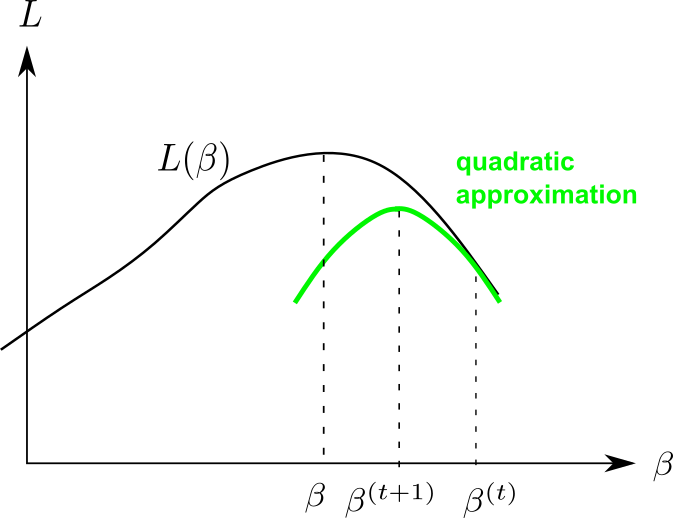
\includegraphics[width=3in]
{gen-lin-mod/gen-lin-mod.png}
\caption{One cycle of Newton-Raphson method
for calculating an estimate $\HAT{\beta}$ for the GLM.}
\label{fig-gml-new-rap}
\end{figure}




\begin{claim}

\beq
\pder{ LL_{\s}}{\beta_{j}}=
 \frac{[y_\s - b'(\xbeta)]}{\av{y_\s, y_\s}}
 \pder{\HAT{\mu}_\s}{\xbeta}
X_{\s, j}
\eeq
\end{claim}
\proof


\beq
\pder{ LL_{\s}}{\beta_{j}}
=
\pder{ LL_{\s}}{\theta_\s}\pder{\theta_\s}{\mu_\s}
\pder{\HAT{\mu}_\s}{\xbeta}\pder{\xbeta}{\beta_{j}}
\eeq

\beq
\pder{ LL_{\s}}{\theta_\s}  =
\frac{y_\s - b'(\theta_\s)}{a(\phi)}
\eeq

\beq
\pder{\mu_\s} {\theta_\s}
=
b''(\theta_\s) = \frac{\av{y_\s, y_\s}}{a(\phi)}
\eeq

\beq
\pder{\HAT{\mu}_\s}{\xbeta} =
(g^{-1})'(\xbeta)
\eeq

\beq
\pder{\xbeta}{\beta_{j}}= X_{\s, j}
\eeq

\beq
\pder{ LL_{\s}}{\beta_{j}}
=
\frac{[y_\s - b'(\theta_\s)]}{\av{y_\s, y_\s}}
 \pder{\HAT{\mu}_\s}{\xbeta}
X_{\s, j}
\eeq

 \qed



\begin{claim}
(Asymptotic expression
for $\av{\HAT{\beta},\HAT{\beta}^T}$
for GLM)


\beq
\av{\HAT{\beta},\HAT{\beta}^T}
\rarrow \cali^{-1}\quad   \text{(asymptotic covariance)}
\eeq
(Hence, more information $\cali$ yields a smaller variance.)
where

\beq
\cali = X^T W X
\eeq
and

\beq
W_{\s, \s'} = \left[\left(\pder{\HAT{\mu}}{\xbeta} \right )^2
\frac{\delta(\s, \s')}
{\av{y_\s, y_\s} } \right]_{\beta=\HAT{\beta}}
\eeq
$\cali$ is called the {\bf information matrix}.

\end{claim}
\proof

\begin{align}
\av{\pder{ LL_\s}{\beta_ { j}}
\pder{ LL_\s}{\beta_ { j'}} }
&=
\av{
\frac{[y_\s - b'(\xbeta)]}{\av{y_\s, y_\s}}
 \pder{\HAT{\mu}_\s}{\xbeta}
X_{\s, j}
\frac{[y_\s - b'(\xbeta)]}{\av{y_\s, y_\s}}
 \pder{\HAT{\mu}_\s}{\xbeta}
X_{\s, j'}
}
\\
&=
 \left[\pder{\HAT{\mu}_\s}{\xbeta}\right]^2
\frac{X_{\s, j} X_{\s, j'}}{\av{y_\s, y_\s}}
\end{align}

\beq
\sum_{\s}
\av{\pder{ LL_{\s}}{\beta_ { j}}
\pder{ LL_{\s}}{\beta_ { j'}} }
=
(X^T W X)_{j, j'}
\eeq
By Section \ref{sec-ent-like-connect}, we have
\beq
\av{\frac{\partial^2 LL_\s}{\partial\beta_ { j}\partial\beta_ { j'}} }
=
-\av{\pder{ LL_\s}{\beta_ { j}}
\pder{ LL_\s}{\beta_ { j'}} }
\eeq
Summing both sides of the last equation over $\s$, we find

\beq
\av{\frac{\partial^2 LL}{\partial\beta_ { j}\partial\beta_ { j'}} }
=
-(X^T W X)_{j, j'}
\eeq
According to  Section \ref{sec-ent-like-connect}, we have
\beq
\av{\HAT{\beta}, \HAT{\beta}^T}\rarrow (X^T W X)^{-1}
\eeq

\qed

\chapter{Generative Adversarial Networks
 (GANs)}
%\begin{refsection}

\begin{figure}[h!]
\centering
\includegraphics[width=6in]{gan/gan.png}
\caption{Generative Adversarial  Network (GAN)} 
\label{fig-gan}
\end{figure}

\begin{figure}[h!]
\centering
\includegraphics[width=6in]{gan/gan-detail.png}
\caption{Discriminator node $\ul{V}$ in Fig.\ref{fig-gan} can be
split into 3 nodes $\vec{\rvc}$, $\vec{\rvd}$ and $\ul{V}$.} 
\label{fig-gan-detail}
\end{figure}

Original GAN, 
Ref.\cite{gf2014}(2014). 

Generator $G$ (counterfeiter) generates samples $\vecf$ of fake money and submits them to Discriminator $D$ (Treasury agent). $D$ also gets samples $\vecr$ of real money. $D$ submits veredict $V\in [0,1]$. $G$ depends on parameter $\theta_G$ and $D$ on parameter $\theta_D$. Veredict $V$ and initial $\theta_G, \theta_D$ are used to get new parameters $\theta'_G, \theta'_D$.Process is repeated (Dynamical Bayesian Network) until saddle point in $V(\theta_G, \theta_D)$ is reached. $D$ makes $G$ better and vice versa.  Zero-sum game between $D$ and $G$.



Let $\cald$ be the domain of $D(\cdot, \theta_D)$. Assume that for any $x\in \cald$,

\beq
0\leq D(x,\theta_D)\leq 1
\;.
\eeq
For any $S\subset\cald$, define

\beq
\sum_{x\in S}D(x,\theta_D)=\lam(S,\theta_D)
\;.
\eeq


 In general, 
$G(\cdot,\theta_G)$ need not be real valued. 

Assume that for every $u\in S_\rvu$,
 $G(u,\theta_G)=f\in S_\rvf\subset \cald$. Define
\beq
\ol{D}(f,\theta_D)=1-D(f,\theta_D)
\;.
\eeq
Note that

\beq
0\leq\ol{D}(f,\theta_D)\leq 1
\;.
\eeq

Define:

\beq
V(\theta_G, \theta_D) =
\sum_{r}P(r)
\ln D(r, \theta_D)
+ \sum_{u}P(u)\ln
\ol{D}(G(u,\theta_G),\theta_D)
\;.	
\eeq

We want the first variation of $V(\theta_G, \theta_D)$ to vanish.




\beq
\delta V(\theta_G, \theta_D)=0
\;.
\eeq
This implies

\beq
 \partial_{\theta_G}V(\theta_G, \theta_D)=
 \partial_{\theta_D}V(\theta_G, \theta_D)=0
\;
\eeq
and

\beq
V_{opt}=\min_{\theta_G}\max_{\theta_D} V(\theta_G, \theta_D)
\;.
\eeq

Node TPMs
for Figs.\ref{fig-gan} and \ref{fig-gan-detail} 
are
given next in blue:

\beq\color{blue}
P(\theta_G)=\;{\rm given}
\eeq

\beq\color{blue}
P(\theta_D)=\;{\rm given}
\eeq


\beq\color{blue}
P(\vecu)=\prod_i P(u[i])  \;\;{\rm (usually \;uniform\; distribution)}
\eeq

\beq\color{blue}
P(\vecr)=\prod_i P(r[i])
\eeq


\beq\color{blue}
P(f[i]\cond \vecu, \theta_G)= \delta[f[i], G(u[i],\theta_G)]
\eeq

\beq\color{blue}
P(c[i]\cond \vecf, \theta_D) = \delta(c[i], \ol{D}(f[i], \theta_D))
\eeq

\beq\color{blue}
P(d[j]\cond \vecr, \theta_D)= \delta(d[j], D(r[j], \theta_D))
\eeq




\beq\color{blue}
P(V| \vecd,  \vecc)=
\delta(V, \frac{1}{N}\ln \prod_{i,j}(c[i]d[j]))
\eeq
where $N=nsam(\vecr)nsam(\vecu)$.


Let $\eta_G, \eta_D> 0$. Maximize $V$ wrt $\theta_D$, and
minimize it wrt $\theta_G$.

\beq\color{blue}
P(\theta'_G|V,\theta_G )=
\delta(\theta'_G, \theta_G - \eta_G 
\partial_{\theta_G}V)
\eeq

\beq\color{blue}
P(\theta'_D|V,\theta_D )=
\delta(\theta'_D, \theta_D + \eta_D 
\partial_{\theta_D}V)
\eeq

\hrule
\begin{figure}[h!]
\centering
\includegraphics[width=2in]{gan/gan-emulate.png}
\caption{GAN, Constraining Bayesian Network}
\label{fig-gan-emulate} 
\end{figure}

Constraining B net given in Fig.\ref{fig-gan-emulate}. It adds 2 new nodes, namely $\ul{\vec{U}}$ and $\ul{\vec{R}}$, to  the bnet of Fig.\ref{fig-gan}. The purpose of these 2  barren (childrenless) nodes is to constrain certain functions to be probability distributions.

Node TPMs for the 2 new nodes given next in blue.


\beq\color{blue}
P(U[i]\cond \theta_G)= 
\frac{\ol{D}(G(U[i],\theta_G),\theta_D))}
{\ol{\lam}(\theta_G, \theta_D)}
\eeq
where  $S_{\ul{U[i]}}=S_\rvu$ and $\ol{\lam}(\theta_G, \theta_D)=\sum_u\ol{D}(G(u, \theta_G), \theta_D))$.

\beq\color{blue}
P(R[i]\cond \theta_G, \theta_D)= \frac{D(R[i], \theta_D)}{\lam(\theta_D)}
\eeq
where $S_{\ul{R[i]}}=S_\rvr$ and  $\lam(\theta_D)=\sum_r D(r, \theta_D)$.


\beq\color{blue}
P(V| \vecu,  \vecr)=
\delta(V, \frac{1}{N}\ln \prod_{i,j}(
P(\ul{R[i]}=r[i]\cond \theta_G, \theta_D)P(\ul{U[i]}=u[j]\cond \theta_G)))
\eeq
where $N=nsam(\vecr)nsam(\vecu)$.


$\call=$ likelihood
\beqa
\call&=&
P(\vecr, \vecu| \theta_G, \theta_D)\\
&=&
\prod_{i,j}\left[
 \frac{D(r[i], \theta_D)}{\lam(\theta_D)}
\frac{\ol{D}(G(u[j],\theta_G),\theta_D))}
{\ol{\lam}(\theta_G, \theta_D)}
\right]
\eeqa

\beq
\ln \call = N[V(\theta_G, \theta_D)
-\ln \lam(\theta_D)-\ln \ol{\lam}(\theta_G, \theta_D)]
\eeq



%\printbibliography[heading=subbibliography]
%\end{refsection}


 
\chapter{Goodness of Causal Fit}
\label{ch-good-causal-fit}
See my paper 
and software Ref.\cite{tucci-gcf}.

\chapter{Granger Causality}
\label{ch-granger-c}

This chapter is based 
on the Wikipedia article 
Ref.\cite{wiki-granger-c}
and Scholarpedia article Ref.\cite{scho-granger-c}
on Granger causality and on
the book  Ref.\cite{hamilton2020time}
on time series analysis by Hamilton.

This chapter assumes the
reader has read Chapter \ref{ch-time-arma}
on the stationary time series $ARMA(p,q)$
and $VAR(p)$.

\begin{figure}[h!]
\centering
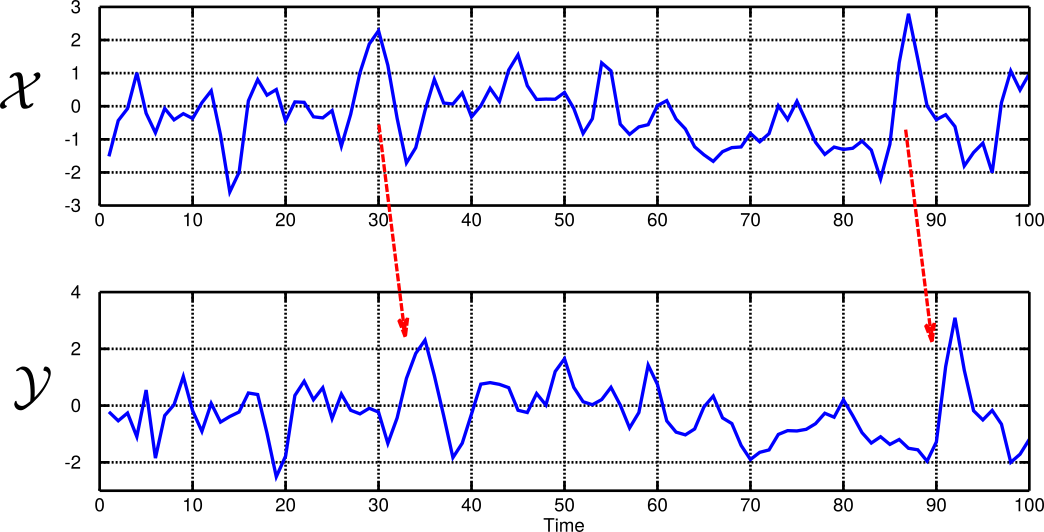
\includegraphics[width=5in]
{granger-c/g-causes.png}
\caption{When t-series $\calx$ Granger-causes
 t-series $\caly$, the patterns in 
$\calx$ are approximately repeated in $\caly$ 
after some time lag (two examples 
are indicated with arrows). Thus, 
past values of $\calx$ can be used for 
the prediction of future values of $\caly$.
(image and caption from Ref.\cite{wiki-granger-c})} 
\label{fig-g-causes}
\end{figure}

Let $\vec{\rvx}_t=[\rvx_t^{A}]_{\forall A}\in 
\RR^{nr_1\times 1}$
and
$\vec{\rvy}_t=[\rvy_t^{B}]_{\forall B}\in 
\RR^{nr_2\times 1}$.
Thus,
 $\vec{\rvx}_t$
for each $t$ is a
column vector with $nr_1$ rows,
and
$\vec{\rvy}_t$
for each $t$ is a
column vector with $nr_2$ rows.
Let $nr_1+nr_2=nr$, the total
number of rows.
Consider a vector 
t-series $\tseries{\vec{\rvx}_t, \vec{\rvy}_t}$
of type $VAR(p)$,
as defined by Eq.(\ref{eq-var-2-def}).
To simplify
the notation
of Eq.(\ref{eq-var-2-def}), we are replacing $x^1$ by $x$,
$x^2$ by $y$,
$n^1$ by $n$,
and $n^2$ by $w$.


{\renewcommand{\arraystretch}{1.5}
\beq
\left[
\begin{array}{c}
\rvx_{t}^{A}
\\
\rvy_t^{B}
\end{array}
\right]
=
\sum_{j=1}^p
\left[
\begin{array}{cc}
\alp_{j}^{\rvx|\rvx;A,A'}
&
\alp_{j}^{\rvx|\rvy;A,B'}
\\
\alp_{j}^{\rvy|\rvx;B,A'}
&
\alp_{j}^{\rvy|\rvy;B,B'}
\end{array}
\right]
\left[
\begin{array}{c}
\rvx_{t-j}^{A'}
\\
\rvy_{t-j}^{B'}
\end{array}
\right]
+
\left[
\begin{array}{c}
\rvn_{t}^{A}
\\
\rvw_{t}^{B}
\end{array}
\right]
\eeq
\label{eq-bipartite-var-q}
} 
Hence,

\beq
E_{| \vec{x}_{<t}, \vec{y}_{<t}}
\left[\rvy_{t}^{B}\right]=
\sum_{j=1}^p
\alp_j^{\rvy|\rvx;B,A'}\rvx_{t-j}^{A'}
+
\sum_{j=1}^p
\alp_j^{\rvy|\rvy;B,B'}\rvy_{t-j}^{B'}
\eeq

Let 
$\calx=\tseries{\vec{\rvx}_t}$
and
$\caly=\tseries{\vec{\rvy}_t}$.

We say {\bf $\calx$ does not G-cause
(or does not G-forecast) $\caly$},
and symbolize this by 
$ \calx\Gno \caly$, if

\beq
\alp_j^{\rvy|\rvx;B, A'}=0 \;\;\forall (j, B, A')
\eeq
or, equivalently, 
\beq
E_{| \vec{x}_{<t}, \vec{y}_{<t}}
\left[\rvy_{t}^B\right]
=
E_{| \vec{y}_{<t}}
\left[\rvy_{t}^{B}\right]\;\;\forall (B, t)
\eeq

We say {\bf $\calx$ G-causes (or G-forecasts) $\caly$}
and symbolize this by
$ \calx\Gyes \caly$, if $\calx \Gno \caly$
is false.

\begin{figure}[h!]
$$
\xymatrix{
\cdots
\vec{\rvn}_{t-3}
&\vec{\rvn}_{t-2}
&\vec{\rvn}_{t-1}
&\vec{\rvn}_t\ar[d]^1
&\vec{\rvn}_{t+1}
\cdots
\\
\cdots
\vec{\rvx}_{t-3}
&\vec{\rvx}_{t-2}\ar@/^1.7pc/[rr]^{\alp_2^{\rvx|\rvx}}
\ar@[red][ddrr]_<{\color{red}\alp_2^{\rvy|\rvx}}
&\vec{\rvx}_{t-1}\ar[r]^{\alp_1^{\rvx|\rvx}}
\ar@[red][ddr]_<{\color{red}\alp_1^{\rvy|\rvx}}
&\vec{\rvx}_t
&\vec{\rvx}_{t+1}
\cdots
\\
\\
\cdots
\vec{\rvy}_{t-3}
&\vec{\rvy}_{t-2}\ar@/_1.7pc/[rr]_{\alp^{\rvy|\rvy}_2}
\ar[uurr]^<{\alp_2^{\rvx|\rvy}}
&\vec{\rvy}_{t-1}\ar[r]_{\alp^{\rvy|\rvy}_1}
\ar[uur]^<{\alp^{\rvx|\rvy}_1}
&\vec{\rvy}_t
&\vec{\rvy}_{t+1}
\cdots
\\
\cdots
\vec{\rvw}_{t-3}
&\vec{\rvw}_{t-2}
&\vec{\rvw}_{t-1}
&\vec{\rvw}_t\ar[u]_1
&\vec{\rvw}_{t+1}
\cdots
}$$
\caption{Bnet for $VAR(2)$.
For clarity, we only
show the arrows entering
nodes $\vec{\rvx}_t$ and $\vec{\rvy}_t$.
Remove red arrows 
if $\calx$
does not G-cause $\caly$,
and
keep them if it does.
}
\label{fig-bipartite-var-2}
\end{figure}

Eq.(\ref{eq-bipartite-var-q}) describing
a bipartite $VAR(p)$
t-series can be represented by 
the bnet Fig.\ref{fig-bipartite-var-2}.
The TPMs, printed in blue,
for the two nodes $\vec{x}_t$
and $\vec{y}_t$, are as follows:


\beq\color{blue}
P(\vec{\rvx}_t|\vec{\rvx}_{[t-p, t-1]},
\vec{\rvy}_{[t-p, t-1]}, \vec{n}_{t})=
\prod_A
\indi\left(
\rvx_t^A=
\sum_{j=1}^p\alp_j^{\rvx|\rvx;A,A'}\rvx^{A'}_{t-j}
+
\sum_{j=1}^p\alp_j^{\rvx|\rvy;A,B'}\rvy^{B'}_{t-j}
+n^A_t
\right)
\eeq



\beq\color{blue}
P(\vec{\rvy}_t|\vec{\rvx}_{[t-p, t-1]},
\vec{\rvy}_{[t-p, t-1]}, \vec{w}_{t})=
\prod_B
\indi\left(
\rvy_t^B=
\sum_{j=1}^p
\underbrace{\alp_j^{\rvy|\rvx;B,A'}}
_{0?}\rvx^{A'}_{t-j}
+
\sum_{j=1}^p\alp_j^{\rvy|\rvy;B,B'}\rvy^{B'}_{t-j}
+w^B_t
\right)
\eeq

{\bf Testing for GC}

\begin{itemize}
\item
Consider the datasets

\beq
\cald_\rvx=
\{(t, \vec{x}_{[t-p, t-1]},
\vec{y}_{[t-p, t-1]},
 \boxed{\vec{x}_t}):
 t\}
\eeq

\beq
\cald_\rvy=
\{(t, \vec{x}_{[t-p, t-1]},
\vec{y}_{[t-p, t-1]},
 \boxed{\vec{y}_t}):
 t\}
\eeq
One can do Linear Regression on 
$\cald_\rvx$
with x-variables
$(\vec{x}_{[t-p, t-1]},
\vec{y}_{[t-p, t-1]})$,
y-variable 
$\vec{x}_t$,
and regression coefficients
$\alp^{\rvx|\rvx}_{[1,p]}$,
$\alp^{\rvx|\rvy}_{[1,p]}$.
One can also do
Linear Regression on 
$\cald_\rvy$
with x-variables
$(\vec{x}_{[t-p, t-1]},
\vec{y}_{[t-p, t-1]})$,
y-variable 
$\vec{y}_t$,
and regression coefficients
$\alp^{\rvy|\rvx}_{[1,p]}$,
$\alp^{\rvy|\rvy}_{[1,p]}$.
The LR software 
yields confidence 
intervals for the
regression coefficients.
\item
One can do hypothesis testing
using the Likelihood Ratio Test\footnote{The 
Likelihood Ratio Test is 
discussed in Section
\ref{sec-likelihood-ratio}.}

Null hypothesis $H_0: \calx\Gno \caly$ ,
Alternative hypothesis $H_1: \calx\Gyes \caly$
\item
Test for both $\calx\Gyes \caly$
and $\caly\Gyes\calx$.
\end{itemize}

{\bf Limitations}

It has been remarked that 
G-causality is not true
causality
because, even though
an event A
must precede an event B
in order to cause it,
that does not 
necessarily mean that
A causes B.
I think the 
problem 
with G-causality
is that it 
uses a bnet that
is a good fit for the dataset,
but not necessarily also a good {\it causal} fit
for the experiment.
One can measure the
goodness of causal fit 
of a bnet by doing 
do-intervention
experiments (See Chapter 
\ref{ch-good-causal-fit}).

\chapter{Hidden Markov Model}\label{ch-hmm}

A Hidden Markov Model (HMM) is
 a  generalization of a
Kalman Filter (KF). KFs 
are discussed 
in Chapter \ref{ch-kalman}. The
bnets of HHMs and KFs
bnets are the same.
The only difference is that a
KF assumes
special node
transition matrices.

See Wikipedia article 
Ref.\cite{wiki-hmm} to learn 
about the history 
and many uses of HMMs. This
chapter is based on
Ref.\cite{nuel}.

\begin{figure}[h!]
\centering
$$\xymatrix{
\rvx_0\ar[d]\ar[r]&
\rvx_1\ar[d]\ar[r]&
\rvx_2\ar[d]\ar[r]&
\rvx_3\ar[d]\\
\rvv_0&
\rvv_1&
\rvv_2&
\rvv_3
}$$
\caption{HMM bnet
with $n=4$.}
\label{fig-hmm}
\end{figure}

Suppose 

$\rvv^n=(\rvv_0, \rvv_1, 
\ldots, \rvv_{n-1})$
are $n$ visible nodes that
are measured,
and 

$\rvx^n=(\rvx_0, \rvx_1, 
\ldots, \rvx_{n-1})$
are the $n$ hidden, unmeasurable 
state nodes of a system
that is being monitored.



For the bnet of Fig.\ref{fig-hmm},
one has
\beq
P(x^n, v^n)=\prod_{i=0}^{n-1}
P(x_i|x_{i-1})P(v_i|x_i)
\;,
\eeq
where $x_{-1}=0$.

Let
$x_{<i} =(x_0, x_1, \dots, x_{i-1})$.

For $i=0,1, \dots, n-1$, define

$\calf_i$=future measurements probability

\beq
\calf_i(x_i)=
P(v_{> i}|x_i)
\eeq

$\ol{\calf}_i$= 
past and present measurements  probability

\beq
\ol{\calf}_i(x_i)=
P(v_{<i},v_i, x_i)
\eeq

$\lam_i$=
present measurement probability

\beq
\lam_i(x_i)=
P(v_i|x_i)
\eeq

$\calf_i$, $\ol{\calf}_i$
and $\lam_i$ 
can be represented graphically
as follows:

\beq
\begin{array}{cc}
\calf_i(x_i)
=
\frac{1}
{P(x_i)}
\sum_{x_{>i}}&
\xymatrix{
x_i\ar[r]
&x_{>i}\ar[d]
\\
&v_{>i}
}
\end{array}
\eeq

\beq
\begin{array}{cc}
\ol{\calf}_i(x_i)
=
\sum_{x_{<i}}&
\xymatrix{
x_{<i}\ar[r]\ar[d]
&x_i\ar[d]
\\
v_{<i}&v_i
}
\end{array}
\eeq

\beq
\begin{array}{cc}
\lam_i(x_i)
=
\frac{1}
{P(x_i)}
&
\xymatrix{
x_i\ar[d]
\\
v_{i}
}
\end{array}
\eeq

\begin{claim}
For $i\geq 0$, 
\beq
P(x_i, v^n)=
\ol{\calf}_i(x_i)\calf_i(x_i)
\;.
\eeq
For $i>0$,

\beq
P(x_{i-1},x_i, v^n)=
 \ol{\calf}_{i-1}(x_{i-1})
\lam_i(x_i)P(x_i|x_{i-1})\calf_i(x_i)
\;.
\eeq


\end{claim}
\proof

\beqa
P(x_i,v^n)
&=&
\sum_{x_{< i}}\sum_{x_{> i}}
P(x^n, v^n)
\\
&=&
\sum_{x_{< i}}\sum_{x_{> i}}
P(x^n, v^n|x_i)P(x_i)
\\
&=&
\sum_{x_{< i}}\sum_{x_{> i}}
P(x_{< i}, v_{< i}, v_i|x_i)
P(x_{>i}, v_{>  i}|x_i)
P(x_i)
\\
&=&
P( v_{< i}, v_i|x_i)
P(v_{>  i}|x_i)
P(x_i)
\\
&=&
\ol{\calf}_i(x_i)\calf_i(x_i)
\eeqa

\beqa
P(x_{i-1},x_i,v^n)
&=&
\sum_{x_{< i-1}}\sum_{x_{>i}}
P(x^n, v^n)
\\
&=&
\sum_{x_{< i-1}}\sum_{x_{>i}}
P(x^n, v^n|x_{i-1}, x_i)P(x_{i-1}, x_i)
\\
&=&
\sum_{x_{< i-1}}\sum_{x_{>i}}
P(x_{<i-1}, v_{<i-1}, v_{i-1}|x_{i-1})
P(v_i|x_i)
P(x_{i-1}, x_i)
P(x_{>  i}, v_{> i}|x_i)
\\
&=&
P( v_{<i-1}, v_{i-1}|x_{i-1})
P(v_i|x_i)
P(x_{i-1}, x_i)
P( v_{> i}|x_i)
\\&=&
 \ol{\calf}_{i-1}(x_{i-1})
\lam_i(x_i)
P(x_i|x_{i-1})
\calf_i(x_i)
\eeqa
\qed

\begin{claim}
For $i>0$, $\calf_i$ and
$\ol{\calf}_i$ can be calculated 
recursively as follows:


\beq
\ol{\calf}_i(x_{i})
=
\sum_{x_{i-1}}
\ol{\calf}_{i-1}(x_{i-1})
\lam_i(x_i)
P(x_i|x_{i-1})
\eeq

\beq
\calf_{ i-1}(x_{i-1})
=
\sum_{x_i}\lam_i(x_i)
P(x_i|x_{i-1})
\calf_i(x_{i})
\eeq

\end{claim}
\proof

\beqa
\ol{\calf}_i(x_i)\calf_i(x_i)
&=&
P(x_i, v^n)\\
&=&
\sum_{x_{i-1}}P(x_{i-1},x_i, 
v^n)\\
&=&\sum_{x_{i-1}}
\ol{\calf}_{i-1}(x_{i-1})
\lam_i(x_i)
P(x_i|x_{i-1})\calf_i(x_i)
\eeqa

\beqa
\ol{\calf}_{i-1}(x_{i-1}
)\calf_{i-1}(x_{i-1})
&=&
P(x_{i-1}, v^n)\\
&=&
\sum_{x_i}P(x_{i-1},x_i, 
v^n)\\
&=&\sum_{x_i}
\ol{\calf}_{i-1}(x_{i-1})
\lam_i(x_i)
P(x_i|x_{i-1})\calf_i(x_i)
\eeqa
\qed

\begin{claim}
\beq
P(x_i|x_{i-1}, v^n)=
\frac{\lam_i(x_i)\calf_{i}(x_i)}
{\calf_{i-1}(x_{i-1})}P(x_i|x_{i-1})
\eeq

\beq
P(x_{i-1}|x_i, v^n)=
\frac{\lam_i(x_i)\ol{\calf}_{i-1}(x_{i-1})}
{\ol{\calf}_i(x_{i})}P(x_i|x_{i-1})
\label{eq-update-2}
\eeq
\end{claim}
\proof
\beqa
P(x_i|x_{i-1}, v^n)&=&
\frac{P(x_{i-1}, x_i, v^n)}
{P(x_{i-1}, v^n)}
\\&=&
\frac{
\ol{\calf}_{i-1}(x_{i-1})
\lam_i(x_i)
P(x_i|x_{i-1})\calf_i(x_i)
}{
\ol{\calf}_{i-1}
(x_{i-1})\calf_{i-1}(x_{i-1})
}
\eeqa
Analogous 
proof for Eq.(\ref{eq-update-2}).
\qed


\chapter{Influence Diagrams \& Utility Nodes}
\label{ch-inf-dia}

Influence diagrams are
just arbitrary bnets
enhanced with a 
new kind of node called an utility node.
The rest
of this brief chapter  will 
be devoted to discussing utility nodes.

Suppose $U(x)$ is a deterministic 
function $U:S_\rvx\rarrow \RR$
called the {\bf utility function}.
Then the {\bf expected utility}
is defined as


\beqa
E_\rvU[\rvU]&=&\sum_UP(U)U
\\
&=&\sum_x\sum_U
\underbrace{P(U|x)}_
{\delta[U, U(x)]}P(x)U
\\
&=&
\sum_xP(x)U(x)
\;.
\eeqa

An {\bf utility node}
can be
understood
as a node
composed of 3 simpler bnet nodes.
This
is illustrated in Fig.\ref{fig-util-node}.

\begin{figure}[h!]
\centering
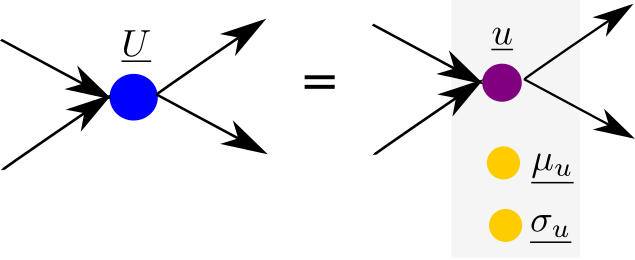
\includegraphics[width=3.5in]
{inf-dia/util-node.png}
\caption{An utility node
can be
understood
as a node 
composed of 3 simpler bnet nodes.} 
\label{fig-util-node}
\end{figure}

The TPMs,
printed in blue,
for the bnet Fig.\ref{fig-util-node},
are as follows:

\beq\color{blue}
P(U|pa(U))=\delta[U, U(pa(U))]
\;,
\eeq
where if $U:S_\rvx\rarrow \RR$,
then $\rvx=pa(\rvU)$.

\beq\color{blue}
P(u|pa(U))=
\delta[u, U(pa(U))]
\eeq

Node $\ul{\mu}_u$
calculates the
expected value (mean value) of $\rvu$:

\beq\color{blue}
P(\mu_u)=\delta(\mu_u,
E_{\rvu}[\rvu])
\eeq

Node $\ul{\sigma}_u$
calculates the
standard deviation of $\rvu$:
\beq\color{blue}
P(\sigma_u)=\delta(\sigma_U,
\sqrt{
E_{\rvu}[
(\rvu-E_{\rvu}[\rvu])^2]})
\eeq

Note that in order to
calculate expected values,
it is necessary that
$\rvU, \rvu\in \RR$. Note that
nodes $\rvu$, $\ul{\mu}_u$, $\ul{\sigma}_u$
must all 3 have access
to the 
TPM
$P(U|pa(U))$ of node $\rvU$.
In fact, in order  to
calculate $E_\rvu[\cdot]$,
it is necessary for
nodes $\ul{\mu}_u$ and 
 $\ul{\sigma}_u$
to have access not just to 
$P(U|pa(U))$ but also to
$P(pa(U))$.

See Fig.\ref{fig-util-merge}.
An influence
diagram may have multiple
utility nodes ($\rvU_1$ and
$\rvU_2$ in Fig.\ref{fig-util-merge}).
Then one can define a merging
utility node $\rvU$ that sums
the values of
all the other utility 
nodes.

\begin{figure}[h!]
\centering
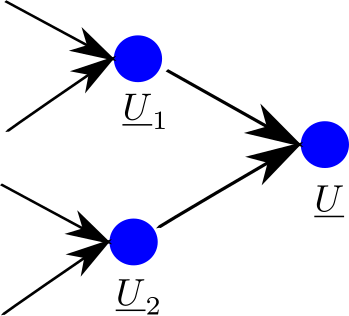
\includegraphics[width=1.5in]
{inf-dia/util-merge.png}
\caption{An influence
diagram may have multiple
utility nodes, say $\rvU_1$ and
$\rvU_2$. Then
one can define an
utility node $\rvU=\rvU_1 + \rvU_2$. } 
\label{fig-util-merge}
\end{figure}

For the node $\rvU$ of 
Fig.\ref{fig-util-merge},
\beq\color{blue}
P(U|U_1, U_2)=\delta(U,U_1 + U_2)
\eeq
\chapter{Instrumental Inequality and beyond}
\label{ch-inst-ineq}

This chapter is based on
Refs. \cite{evans-inst-ineq} and 
\cite{pearl-inst-ineq}.

Instrumental Variables (IVs) 
are discussed in Chapter \ref{ch-instrumental}.
This chapter will discuss
the original Instrumental
inequality (I-inequality)
discovered by Pearl, 
and other related inequalities.
The I-inequality arises
in bnets that use an IV.
The I-inequality bounds
the effect that an IV
$\rvz$
can have on the outcome $\rvy$ of
a treatment $\rvd\rarrow\rvy$.
Since
there is a path
$\rvz\rarrow\rvd\rarrow\rvy$,
the treatment dose $\rvd$
acts as a mediator
between the IV $\rvz$ 
and the treatment outcome $\rvy$.
The I-inequality is reminiscent
of the data processing 
inequality
$H(\rvz:\rvy)\leq H(\rvd:\rvy)$
which is valid
for a simple Markov chain bnet 
$\rvz\rarrow\rvd\rarrow\rvy$.
The data processing
inequality
is saying that
the endpoint $\rvy$
receives 
more information from $\rvd$
than from
$\rvz$. This is reasonable,
since $\rvy$ is ``closer" to $\rvd$ than to
$\rvz$.



\section{I-inequality}

\begin{figure}[h!]
$$
\begin{array}{ccc}
\xymatrix{
&&\rvu\ar@{-->}[dl]\ar@{-->}[dr]
\\
\rvz\ar[r]
&\rvd\ar[rr]&&\rvy
}
&&
\xymatrix{
&&\rvu\ar@{-->}[dl]\ar@{-->}[dr]
\\
\rvz\ar[r]
&\rvd
&\rvtd=\td\ar[r]
&\rvy
}
\\
\\
G&&\TIL{G}=\cali_{\rvd\rarrow\rvy}(\td)G
\end{array}
$$
\caption{In bnet $G$, 
an IV $\rvz$
acts on a treatment $\rvd\rarrow\rvy$.
Bnet $\TIL{G}$
is obtained
by applying
an imagine
operator
to arrow
$\rvd\rarrow\rvy$
of bnet $G$.} 
\label{fig-iv-ineq-im}
\end{figure}

\begin{claim}
The TPMs for the bnet $G$ in 
Fig.\ref{fig-iv-ineq-im}
satisfy

\beq
\max_d \sum_y \max_z
P(d,y|z)
\leq 1
\eeq
\end{claim}
\proof

Below,
any
probability
that alludes
to a value $\td$
refers to bnet $\TIL{G}$.
Otherwise,
if it doesn't allude to $\td$, then
it refers to $G$
(or to $\TIL{G}$,
since the TPMs of $\TIL{G}$
are defined
from those
of $G$
in a consistent manner.)


$G$ satisfies
\beq
P(d,y|z)=\sum_u P(u)
P(y|u, d)P(d|u,z)
\;,
\label{eq-p-d-y-bar-z}
\eeq
and $\TIL{G}$ satisfies

\beq
P(d,y|z, \td)=\sum_u P(u)
P(y|u,\td)P(d|u,z)
\;.
\label{eq-p-d-y-bar-z-tilde}
\eeq
Note that Eqs.(\ref{eq-p-d-y-bar-z})
and
(\ref{eq-p-d-y-bar-z-tilde}) imply that

\beq
P(d,y|z, d)=P(d,y|z)
\eeq
and that


\beq
\boxed{
P(\td, y|z, \td)\leq \sum_d P(d, y|z, \td)
=P(y|\td)
}
\;.
\label{eq-p-td-boxed}
\eeq
Thus,

\beqa
\max_\td \sum_y\max_z P(\td, y|z, \td)
&\leq &\max_\td \sum_y\max_z P(y|\td)
\\
&\leq&\max_\td \sum_yP(y|\td)
\\
&\leq&\max_\td 1
\\
&\leq&1
\eeqa
\qed


As pointed out in Ref.\cite{evans-inst-ineq}
from which
I learned the above
proof,
the above proof
is highly
generalizable.

Fig.\ref{fig-iv-ineq-proof}
gives a graphical
representation
of the boxed
Eq.(\ref{eq-p-td-boxed})
which is crucial
to the proof.

\begin{figure}[h!]
$$
\begin{array}{cccccc}
\sum_u
\xymatrix{
&&\rvu\ar@{-->}[dl]\ar@{-->}[dr]
\\
\rvz\ar[r]
&\rvd=\td
&\rvtd=\td\ar[r]
&\rvy
}&\leq&
\sum_d  \sum_u
\xymatrix{
&&\rvu\ar@{-->}[dl]\ar@{-->}[dr]
\\
\rvz\ar[r]
&\rvd
&\rvtd=\td\ar[r]
&\rvy
}
&=&
\xymatrix{
.
\\
\rvtd=\td\ar[r]
&\rvy
}
\end{array}
$$
\caption{Graphical
representation
of the boxed equation
Eq.(\ref{eq-p-td-boxed}). } 
\label{fig-iv-ineq-proof}
\end{figure}

And here is a 
meta-description
of the steps in the proof:
\begin{enumerate}
\item Use imagine operator to create a
non-negative matrix $M_{d, \td}$.
\item Use fact that row or column sum
of $M_{d, \td}$ is larger than diagonal
element in sum: 
$\sum_d M_{d, \td}\geq M_{\td,\td}$.
\end{enumerate}

\subsection{I-inequality for 
binary z,d,y}


It is enlightening
to write down the
I-inequality 
for the special case that
$\rvz, \rvd, \rvy$
are binary.

\begin{figure}[h!]
\centering
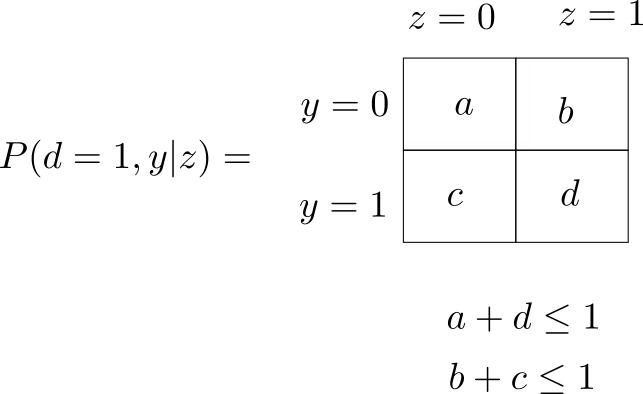
\includegraphics[width=3in]
{inst-ineq/binary-inst-ineq.png}
\caption{I-inequality for 
binary $\rvz, \rvd, \rvy$.
The same picture except with $d=0$
is also true.} 
\label{fig-iv-ineq-binary}
\end{figure}

In the binary case,
the I-inequality implies 4 different inequalities.
These are as follows.
One gets 
two inequalities 
by setting $d=1$ 
in the next 2 equations.

\begin{subequations}
\label{eq-i-ineq-bin}
\beq
\sum_{y=0}^1\sum_{z=0}^1 \indi(y=z) P(d,y|z)
\;,
\eeq

\beq
\sum_{y=0}^1\sum_{z=0}^1 
\indi(y\neq z) P(d,y|z)
\;.
\eeq
\end{subequations}
One gets an additional
2 inequalities by setting $d=0$
in Eqs.(\ref{eq-i-ineq-bin}).
These 4 inequalities
are illustrated in Fig.\ref{fig-iv-ineq-binary}.

What do they mean? That at fixed $\rvd$,
 the correlation
between $\rvz$ and $\rvy$ is limited.


\section{Bounds on 
Effect of IV on treatment
outcome y
}

\begin{figure}[h!]
$$
\begin{array}{ccccc}
\xymatrix{
&&\rvu\ar@{-->}[dl]\ar@{-->}[dr]
\\
\rvz\ar[r]\ar@/_1.5pc/[rrr]
&\rvd\ar[rr]&&\rvy
}
&&
\xymatrix{
&&\rvu\ar@{-->}[dr]
\\
\rvz\ar@/_1.5pc/[rrr]
&\cald\rvd=\td\ar[rr]&&\rvy
}
&&
\xymatrix{
&&\rvu\ar@{-->}[dl]\ar@{-->}[dr]
\\
\rvz\ar[r]\ar@/_1.5pc/[rrr]
&\rvd
&\rvtd=\td\ar[r]
&\rvy
}
\\
\\
\calg&&
\calg_{do}=\cald_{\rvd=\td}\calg
&&\calg_{im}=
\cali_{\rvd\rarrow\rvy}(\td)\calg
\end{array}
$$
\caption{Bnet $\calg$
is obtained
from the bnet $G$
in Fig.\ref{fig-iv-ineq-im}
by adding to $G$ an arrow
from the IV $\rvz$
to the treatment
outcome $\rvy$.
Bnet $\calg_{do}$
is obtained by applying
a do operator
to node $\rvd$ of $\calg$.
Bnet $\calg_{im}$
is obtained by applying
an imagine operator
to arrow $\rvd\rarrow\rvy$ of $\calg$.
} 
\label{fig-iv-ineq-z-y-arc}
\end{figure}
In this section,
we will assume
that random variables
$\rvz, \rvd, \rvy$
are binary.
Just as with
the binary case
of the I-inequality,
we will
find an inequality
for each value
of $\rvd\in \bool$.

Below, we will
use the following 3
shorthand notations:

\beq
P_{y|z}(d)=
P(d,y|z)
\;,
\eeq

\beq
P_{|z}(d)=\sum_y P(d, y|z)
\;,
\eeq
and

\beq
\pi_{|z}(d) = 1-P_{|z}(d)
\;.
\eeq

For the bnet $\calg_{do}$
in Fig.\ref{fig-iv-ineq-z-y-arc},
define the IV effect at
fixed  $\cald\rvd=\td$ by
\beq
IVE(\td)=
P(y=1|z=1, \cald\rvd=\td)-
P(y=1|z=0, \cald\rvd=\td)
\;.
\eeq

\begin{claim}
The TPMs for the bnet $\calg_{do}$
in Fig.\ref{fig-iv-ineq-z-y-arc}
 satisfy

\beq
\pi_{|0}(d)\leq\left[
IVE(d)-\{P_{1|1}(d)-P_{1|0}(d)\}\right]\leq \pi_{|1}(d)
\eeq
\end{claim}
\proof
\beqa
P(y|z, \cald\rvd=\td)
&=&
\sum_u P(u) P(y|u,z, \td)
\\
&=&
\sum_u P(u)\sum_d P(d,y|u,z, \td)
\\
&\geq&
\sum_u P(u)P(\td,y|u,z, \td)
\\
&=&
\sum_u P(u)P(\td,y|u,z)
\\
&=&
P_{y|z}(\td)
\eeqa

Next note that $P(d, y|z, \td)\geq 0$,
and  
$\sum_{d,y}P(d, y|z, \td)=1$.
If we write
a table for 
$P(d, y|z, \td)$ 
at fixed $z,\td$
with row 
and
column indices $(d, y)$,
then
a partial
sum of the entries of that
table must be $\leq 1$:

\beq
\sum_{d\neq \td}P(d, y|z, \td)
+
\underbrace{\sum_{y'}P(\td,y'|z, \td)}_{P_{|z}(\td)}
\leq 1
\;.
\eeq
Using the definitions
of $P_ {|z}$ and $\pi_{|z}$,
we can rewrite the last
equation as 

\beq
\sum_{d\neq \td}P(d,y|z, \td)
\leq
\pi_{|z}(\td)
\;.
\eeq

Next note that

\beqa
P(y|z, \cald\rvd=\td)
&=&
\sum_u P(u) P(y|u,z, \td)
\\
&=&
\sum_u P(u)\sum_d P(d,y|u,z, \td)
\\
&=&
 P(\td,y|z, \td)+\sum_{d\neq \td} P(d,y|z, \td)
\\
&=&
P_{y|z}(\td)
+
\sum_{d\neq\td} P(d,y|z,\td)
\\
&\leq&
P_{y|z}(\td)
+ \pi_{|z}(\td)
\;.
\eeqa
Hence,

\beq
P_{y|z}(\td)\leq P(y|z, \cald\rvd=\td)\leq P_{y|z}(\td)
 + \pi_{|z}
\eeq

\beq
P_{1|1}(\td)\leq P(y=1|z=1, \cald\rvd=\td)\leq P_{1|1}(\td)
+ \pi_{|1}
\eeq

\beq
-P_{1|0}(\td) -\pi_{|0} \leq -P(y=1|z=0, \cald\rvd=\td)\leq- P_{1|0}(\td)
\eeq
\qed



\chapter{Instrumental Variables}
\label{ch-instrumental}


This chapter is based on
Refs.\cite{book-mixtape} and \cite{wiki-inst-vars}.

The theory of potential outcomes (PO)
discussed in Chapter \ref{ch-po}
assumes that confounders can be ignored
by conditioning on them.
However, there are cases when
that is not possible, as when there are some
unmeasured (i.e., unobserved, hidden)
confounder nodes in the bnet,
because one can
only condition on observed random 
variables, by definition.
So what if confounders can't be ignored?
Are we then precluded from using PO theory?
Not necessarily.
It might still be possible to
use PO theory if one can find a suitable
instrumental variable (IV) for the problem.

IVs were actually invented 
by Sewall Wright and his father Philip
Wright long before
PO theory was invented  by Rubin.
The reason why IVs save PO theory
is greatly clarified by using
Pearl causal DAGs and his d-separation theorem 
(see Chapter \ref{ch-dsep}).

Most of the discussion in this chapter
is  limited to LDEN (linear deterministic
bnets with external noise). These
are discussed in Chapter \ref{ch-linear-sys}.
However, as will become
obvious to the reader, IVs are 
also applicable
and useful
in general bnet modeling.



\section{$\delta$ with unnmeasured confounder}

In this section,
we explain using LDENs 
why
unmeasured confounders 
prejudice PO calculations.

\begin{figure}[h!]
$$
\xymatrix{
&\rvh\ar@{-->}[dl]_\nu\ar@{-->}[dr]^\mu
\\
\rvd\ar[rr]_\delta&&\rvy
}$$
\caption{An LDEN bnet. The direct path $\rvd\rarrow\rvy$
is confounded by
a hidden variable $\rvh$.
} 
\label{fig-iv-G-start}
\end{figure}

Consider 
the LDEN bnet of Fig.\ref{fig-iv-G-start},
For some $\delta, \mu\in \RR$, we have

\beq
\rvy = \delta \rvd +
\underbrace{ \mu \rvh + \rvu_\rvy}_{\rvn_y}
\;.
\eeq
If $\av{\rvn_\rvy, \rvd}=0$, then

\beq
\av{\rvy, \rvd} = \delta_0 \av{\rvd, \rvd}
\;,
\eeq
whereas if
$\av{\rvn_\rvy, \rvd}\neq 0$, then

\beq
\av{\rvy, \rvd} = \delta_1 \av{\rvd, \rvd}
+ \av{\rvn_\rvy, \rvd}
\;.
\eeq
Therefore,


\beq
\delta_0 = \frac{\av{\rvy, \rvd}}{\av{\rvd, \rvd}}
\;,
\eeq

\beq
\delta_1 =
\underbrace{\frac{\av{\rvy, \rvd}}{\av{\rvd, \rvd}}}_{\delta_0}
-
\frac{\av{\rvn_\rvy, \rvd}}{\av{\rvd, \rvd}}
\;.
\eeq  
If we assume no confounders
and there is one, this gives the difference
between the estimate $\delta_1$ of $\delta$ for
the truth, versus
the naive estimate $\delta_0$.

If the confounder $\rvh$
had been measured, then
we would calculate 
the covariances at fixed $\rvn_\rvy$,
and 
the conditional covariance 
$\av{\rvn_\rvy, \rvd}_{|\rvn_\rvy}=0$

\section{$\delta$
(with unmeasured confounder)
can be
inferred via IV}



\begin{figure}[h!]
$$
\begin{array}{ccc}
\xymatrix{
&&\rvh\ar@{-->}[dl]_\nu\ar@{-->}[dr]^\mu
\\
\rvA\ar[r]_\alpha
&\rvd\ar[rr]_\delta
&&\rvy
}
&&
\xymatrix{
&&\rvh\ar@{-->}[dl]_\nu\ar@{-->}[dr]^\mu
\\
\rvA\ar[r]_\alpha
&\rvd&
\rvtd\ar[r]_\delta
&\rvy}
\\
\\
G&&G_{im+}
\end{array}
$$
\caption{
Two LDEN bnets. The direct path $\rvd\rarrow\rvy$
is confounded by
a hidden variable $\rvh$, but
by using the IV $\rvA$, we are still
able to 
identify (i.e. calculate)
$\delta$.
}
\label{fig-iv-G-im}
\end{figure}

Now consider the two LDEN bnets 
shown in Fig.\ref{fig-iv-G-im}.
Note that there are no arrows
$\rvA\rarrow\rvy$
or 
$\rvA\rarrow\rvh$. Note that
node $\rvd$ is a collider
in the path 
$\rvA-\rvd-\rvh-\rvy$, 
Therefore,
the only unblocked path
from $\rvA$ to 
$\rvy$ in G 
is $\rvA\rarrow\rvd\rarrow\rvy$
and that path has been
removed in $G_{im+}$. These
observations are 
encapsulated in the following statements.

\beq
\rvd\perp_{G} \rvy =\text{false}, 
\;\; \rvA\perp_{G} \rvy= \text{false}
\;.
\eeq

\beq
\rvd\perp_{G_{im+}} \rvy =\text{false}, 
\;\; \rvA\perp_{G_{im+}} \rvy= \text{true}
\;.
\eeq


The following is true for $G$:

\beq
\rvy = \delta\rvd + 
\underbrace{\mu\rvh + \rvu_\rvy}_
{\rvn_\rvy}
\eeq

\beq
\rvd= \alp \rvA + 
\underbrace{\nu\rvh + \rvu_\rvd}
_{\rvn_\rvd}
\;.
\eeq

Since 
$\av{\rvn_\rvy, \rvA}=\av{\rvn_\rvd, \rvA}=0$
is true in $G$, we have
\beq
\av{\rvy, \rvA}= \delta \av{\rvd, \rvA}
\;
\eeq
and

\beq
\av{\rvd, \rvA}= \alp \av{\rvA, \rvA}
\;.
\eeq
Note that $\av{\rvy, \rvA}=\delta=0$
for $G_{im+}$
but not for $G$,
so we are speaking about $G$
from here on. It 
follows that



\beq
\alp=\frac{ \av{\rvd, \rvA}}{ \av{\rvA, \rvA}}
\eeq
and

\beqa
\delta&=&\frac{ \av{\rvy, \rvA}}{ \av{\rvd, \rvA}}
\\
&=&
\frac{ \av{\rvy, \rvA}}{ \av{\rvA, \rvA}}
\frac{\av{\rvA, \rvA}}{ \av{\rvd, \rvA}}
\\
&=&
\frac{ \av{\rvy, \rvA}}{ \av{\rvA, \rvA}}
\frac{1}{\alp}
\\
&=&
\frac{ \av{\rvy, \alp\rvA}}{ \av{\alp\rvA,\alp \rvA}}
\;.
\eeqa

\section{More general bnets with IVs}

\begin{figure}[h!]
$$
\begin{array}{ccc}
\xymatrix{
&&\rvh\ar@{-->}[dl]\ar@{-->}[dr]
\\
\rvA\ar[r]\ar[drr]
&\rvd\ar[rr]_\delta
&&\rvy\ar[dl]
\\
&&\rvv
}
&&
\xymatrix{
&&\rvh\ar@{-->}[dl]\ar@{-->}[dr]
\\
\rvA\ar[r]\ar[drr]
&\rvd&
\rvtd\ar[r]_\delta
&\rvy\ar[dl]
\\
&&\rvv
}
\\
\\
G&&G_{im+}
\end{array}
$$
\caption{The 2 paths in $G_{im+}$
from
IV variable $\rvA$
to $\rvy$ are blocked by colliders $\rvv$ 
and $\rvd$. Thus,
$
\rvd\perp_{G_{im+}} \rvy =\text{false}, 
\;\; \rvA\perp_{G_{im+}} \rvy= \text{true}
$
}
\label{fig-iv-G-im-blocked}
\end{figure}




\begin{figure}[h!]
$$
\begin{array}{ccc}
\xymatrix{
&&\rvh\ar@{-->}[dl]\ar@{-->}[dr]
\\
\rvA\ar[r]
&\rvd\ar[rr]_\delta
&&\rvy
\\
&&\rvv\ar[ur]\ar[ull]
}
&&
\xymatrix{
&&\rvh\ar@{-->}[dl]\ar@{-->}[dr]
\\
\rvA\ar[r]
&\rvd
&
\rvtd\ar[r]_\delta
&\rvy
\\
&&\rvv\ar[ur]\ar[ull]
}
\\
\\
G&&G_{im+}
\end{array}
$$
\caption{
There are 2 paths in $G_{im+}$
from
IV variable $\rvA$
to $\rvy$. One is
blocked
by the collider $\rvd$
and the other
can be blocked by 
conditioning on $\rvv$. Thus,
$
\rvd\perp_{G_{im+}} \rvy|\rvv =\text{false}, 
\;\; \rvA\perp_{G_{im+}} \rvy|\rvv= \text{true}
$
}
\label{fig-iv-G-im-strata}
\end{figure}

Figs.\ref{fig-iv-G-im-blocked}
and \ref{fig-iv-G-im-strata}
are examples of 
other bnets 
for which the
effect $\delta$
is identifiable
thanks
to the
IV $\rvA$.


\section{Instrumental Inequality}
Pearl's instrumental inequality
and related inequalities are discussed in
 Chapter
 \ref{ch-inst-ineq}.



%
\chapter{IN PROGRESS: Generative Adversarial Networks, Ensemble GANs}
\begin{refsection}
Bayesian GAN, 
 Ref.\cite{wilson2017} (2017)

Replace $\theta_a$ by $\vtheta_a$ and 
$\theta'_a$ by $\vtheta'_a$ for $a=G,D$



\beq
\delta V(\vtheta_G, \vtheta_D)=0
\eeq

\beq
 \partial_{\vtheta_G}V(\vtheta_G, \vtheta_D)=
 \partial_{\vtheta_D}V(\vtheta_G, \vtheta_D)=0
\eeq

\beq
V_{opt}=\min_{\vtheta_G}\max_{\vtheta_D} V(\vtheta_G, \vtheta_D)
\eeq

\beq
P(\vtheta_G)=\prod_i P(\theta_G[i])
\eeq

\beq
P(\vtheta_D)=\prod_i P(\theta_D[i])
\eeq


\beq
P(\vecu)=\prod_i P(u[i])
\eeq

\beq
P(\vecr)=\prod_i P(r[i])
\eeq


\beq
P(f[i]|\vecu, \vtheta_G)= \prod_i\delta[f[i], G(u[i],\vtheta_G)]
\eeq

\beq
P(c[i]|\vecf, \vtheta_D) = \delta(c[i], \ol{D}(f[i], \vtheta_D))
\eeq

\beq
P(d[j]|\vecr, \vtheta_D)= \delta(d[j], D(r[j], \vtheta_D))
\eeq


\beq
P(V| \vecd,  \vecc)=
\delta(V, \frac{1}{N}\ln \prod_{i,j}(c[i]d[j]))
\eeq
where $N=nsam(\rvr)nsam(\rvu)$







$\eta_G, \eta_D> 0$, maximize wrt $\theta_D$, 
minimize wrt $\theta_G$
\beq
P(\theta'_G|V,\vtheta_G )=
\delta(\vtheta'_G, \vtheta_G - \eta_G 
\partial_{\vtheta_G}V)
\eeq

\beq
P(\theta'_D|V,\vtheta_D )=
\delta(\vtheta'_D, \vtheta_D + \eta_D 
\partial_{\vtheta_D}V)
\eeq


\hrule
Emulated B net

\beq
P(\vtheta_G)=\;\prod_i P(\theta_G[i])
\eeq

\beq
P(\vtheta_D)=\;\prod_i P(\theta_D[i])
\eeq


\beq
P(u[i]|\vtheta_G, \vtheta_D)=  
\ol{D}(G(u[i],\vtheta_G), \vtheta_D)
\eeq


\beq
P(r[i]|\vtheta_D)=  
D(r[i], \vtheta_D)
\eeq

\beq
P(V| \vecd,  \vecc)=
\delta(V, \prod_{i,j,a,b}(u[i]r[j]\theta_G[a]\theta_D[b]))
\eeq



$\eta_G, \eta_D > 0$, maximize wrt $\theta_D$, 
minimize wrt $\theta_G$
\beq
P(\vtheta'_G|V,\vtheta_G )=
\prod_i \delta(\theta'_G[i], \theta_G[i] - \eta_G 
\partial_{\theta_G[i]}\ln V)
\eeq

\beq
P(\vtheta'_D|V,\vtheta_D )=\prod_i
\delta(\theta'_D[i], \theta_D[i] + \eta_D 
\partial_{\theta_D[i]}\ln V)
\eeq

\beq
P(\vecr, \vecu, \vtheta_G, \vtheta_D)=
\prod_{i,j,a,b}
\left\{
P(\theta_G[a])P(\theta_D[b])\\
 \frac{D(r[i], \theta_D[b])}{\lam(\theta_D[b])}
\frac{\ol{D}(G(u[j],\theta_G[a]),\theta_D[b]))}
{\ol{\lam}(\theta_G[a], \theta_D[b])}
\right\}
\eeq


$N=nsam(\vecr)nsam(\vecu)
nsam(\vtheta_G)nsam(\vtheta_D)$

\beq
\ln P(\vecr, \vecu, \vtheta_G, \vtheta_D) =
N\left\{
\begin{array}{l}
-H(P_{\ul{\theta}_D})+ \sum_{r,\theta_D}P(r)P(\theta_D)
\ln \frac{D(r, \theta_D)}{\lam(\theta_D)}
\\
-H(P_{\ul{\theta}_G})+ \sum_{u,\theta_G,\theta_D}P(u)
P(\theta_G)P(\theta_D)\ln
\frac{\ol{D}(G(u,\theta_G),\theta_D)}{\ol{\lam}(\theta_G, \theta_D)}
\end{array}
\right.
\eeq

\beq
\ln P(\vecr, \vecu) =
N\left\{
\begin{array}{l}
 \sum_{r}P(r)
\ln \sum_{\theta_D}P(\theta_D)\frac{D(r, \theta_D)}{\lam(\theta_D)}
\\
+ \sum_{u}P(u)
\ln \sum_{\theta_D, \theta_G}
P(\theta_G)P(\theta_D)
\frac{\ol{D}(G(u,\theta_G),\theta_D)}{\ol{\lam}(\theta_G, \theta_D)}
\end{array}
\right.
\eeq

\beqa
V(\vtheta_G, \vtheta_D) &=&\frac{1}{N} \ln P(\vtheta_G, \vtheta_D|\vecr,\vecu,)\\&=&
\frac{1}{N} [
\ln P(\vecr,\vecu,\vtheta_G, \vtheta_D)
-\ln P(\vecr,\vecu)]
\eeqa



\printbibliography[heading=subbibliography]
\end{refsection}


\chapter{Jackknife Resampling}\label{ch-jack}

This chapter is based on
Ref. \cite{wiki-jack}.

Before reading this chapter,
we recommend that you
read the section entitled
\qt{Demystifying
Population and Sample
Variances}, in
Chapter \ref{ch-conventions}.

{\bf Jackknife resampling} (JR) is a statistical technique used to estimate the precision or bias of sample statistics, like the mean, variance, and standard error. It involves creating from a list of
$n$ samples, $n$ new lists
with $n-1$ samples each. The new
lists are created by leaving out one different sample each time.
One can then relate
the statistics of those $n$ new lists with the statistics of the 
original list.
This technique is called JR because, like
a jackknife,
it has multiple applications,
such as variance estimation, bias correction and influence analysis. 



Let $\Sigma=\{0,1,2, \ldots, n-1\}$.
Let us consider the list of samples

\beq
x^n=(x^\s)_{\s\in\Sigma}
\;,
\eeq
where the $x^\s$ are assumed to be i.i.d. with


\beq
E[\rvx^\s]=\mu
\eeq
and

\beq
\av{\rvx^\s, \rvx^{\s'}}=V_1\delta(\s, \s')
\;.
\eeq
If we define $\mu$ and $V_1$
 estimators by

\begin{subequations}
\label{eq-jr-xs-estimators}
\beq
\HAT{\mu}=\frac{1}{n}\sum_\s x^\s
\eeq

\beq
\HAT{V}_1=
\frac{1}{n-1}\sum_\s (x^\s-\HAT{\mu})^2
\;,
\eeq
\end{subequations}
then one can show that:

\beq
E[\ul{\HAT{\mu}}]=\mu\;,\;\;E[\HAT{\rvV}_1]=V_1
\eeq
so both of these estimators are unbiased.

Now define lists
of samples with one
of the items in $x^n$ deleted:

\beq
x^{n-1}_\xi=(x^\s)_{\s\in\Sigma-\{\xi\}}
\;.
\label{eq-def-vec-x-xi}
\eeq

Suppose we are given functions
of $x^n$ and $x^{n-1}_\xi$

\beq
A=\Phi(x^n; n)
\;,
\eeq

\beq
A_\xi=\Phi(x^{n-1}_\xi; n-1)
\;.
\label{eq-def-a-xi}
\eeq
Then define a list $A^n$ by
\beq
A^n=(A_\xi)_{\xi\in \Sigma}
\;.
\eeq
One can also define a list
$B^n$ by:

\beq
B^n=
(B_\xi)_{\xi\in \Sigma}
\eeq
where

\beqa
B_\xi&=&
nA-(n-1)A_\xi\\
&=&
A_\xi
-n[A_\xi-A]
\;.
\label{eq-def-b-xi}
\eeqa
Later on,
we will see why
the list $B^n$
 is of
interest.

\begin{figure}[h!]
$$
\xymatrix{
&\rvx^n
\ar[lddd]
\ar[d]\ar[dr]\ar[drr]
\\
&\rvx^{n-1}_0\ar[d]
&\rvx^{n-1}_1\ar[d]
&\rvx^{n-1}_2\ar[d]
\\
&\rvA_0\ar[d]
&\rvA_1\ar[d]
&\rvA_2\ar[d]
\\
\rvA\ar[r]
\ar@/_1pc/[rr]
\ar@/_1pc/[rrr]
&\rvB_0
&\rvB_1
&\rvB_2
}
$$
\caption{Bnet for jackknife resampling (JR).}
\label{fig-jack-bnet}
\end{figure}

Fig.\ref{fig-jack-bnet}
is a bnet
that encapsulates JR.
The TPMs, printed in blue,
for that bnet,
are as follows:

\beq\color{blue}
P(x^{n-1}_\xi|x^n)=
\indi(\;\;\;
x^{n-1}_\xi= \text{ defined by Eq.(\ref{eq-def-vec-x-xi})}
\;\;\;)
\eeq

\beq\color{blue}
P(A_\xi|x^{n-1}_\xi)=
\indi(\;\;\;
A_\xi= \text{ defined by Eq.(\ref{eq-def-a-xi})}
\;\;\;)
\eeq

\beq\color{blue}
P(B_\xi|A_\xi, A)=
\indi(\;\;\;
B_\xi= \text{ defined by Eq.(\ref{eq-def-b-xi})}
\;\;\;)
\eeq



\section{Case
$A=\Phi(x^n; n)=\frac{1}{n}
\sum_\sigma x^\sigma$}

Suppose

\beq
A=
\underbrace{\frac{1}{n}\sum_\s x^\s}_
{ E_\s[x^\s]}
\eeq
and

\beq
A_\xi=
\underbrace{\frac{1}{n-1}
\sum_{\s\in \Sigma-\{\xi\}}
 x^\s}_
{E_{\s|\xi}[x^\s]\text{ where } P(\s|\xi)=\frac{\indi(\s\neq\xi)}{n-1}}
\;.
\eeq
Then

\beq
\frac{1}{n}
\sum_\xi
A_\xi=E_\xi E_{\s|\xi}[x^\s]=E_\s[x^\s]=A
\eeq

\begin{claim}
\beq
E[\rvA_\xi]=\mu
\eeq

\beq
\av{\rvA_\xi, \rvA_{\xi'}}=
V_1
\left[
\frac{n-2-\delta(\xi, \xi')}{(n-1)^2}
\right]
\eeq
\end{claim}
\proof
\beqa
E[\rvA_\xi]=\frac{1}{n-1}\sum_\s \indi(\xi\neq\s)E[\rvx^\s]=\mu
\eeqa

\beqa
\av{\rvA_\xi, \rvA_{\xi'}}&=&
\frac{1}{(n-1)^2}
\sum_\s\sum_{\s'}
[1-\delta(\s, \xi)]
[1-\delta(\s', \xi')]\av{x^\s, x^{\s'}}
\\
&=&
\frac{V_1}{(n-1)^2}
\sum_\s\sum_{\s'}
[1-\delta^\s_\xi-\delta^{\s'}_{\xi'}
+
\delta^\s_\xi\delta^{\s'}_{\xi'}]\delta^\s_{\s'}
\\
&=&
\frac{V_1}{(n-1)^2}
[n-2+\delta^\xi_{\xi'}]
\eeqa
\qed

\begin{figure}[h!]
\centering
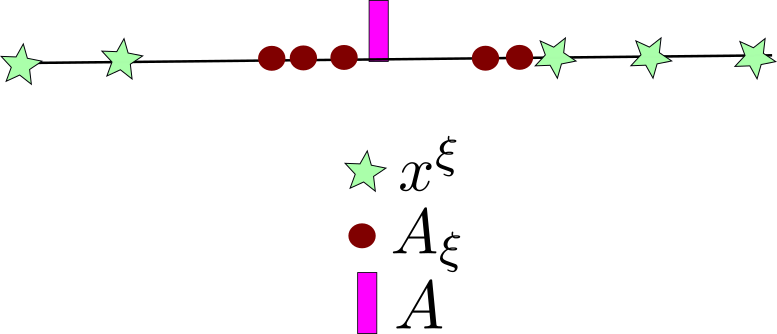
\includegraphics[width=2in]
{jack/jack-dots.png}
\caption{For each
point $x^\xi$,
there  is a corresponding point
$A_\xi$
which is $n-1$ times closer to the average $A$
than $x^\xi$ is.}
\label{fig-jack-dots}
\end{figure}

\begin{claim}
\beq
A_\xi-A=
\frac{A-x^\xi}{n-1}
\label{eq-prox-to-A}
\eeq
Hence, the distance of a point
$x^\xi$ to the mean value  $A$
is $n-1$ times as large
as the distance of $A_\xi$ to $A$.
(see Fig.\ref{fig-jack-dots})
\end{claim}
\proof
\beqa
A_\xi-A
&=&
\frac{1}{n-1}
\left(\sum_\s x^\s - x^\xi\right)
-
\frac{1}{n}\sum_\s x^\s
\\
&=&
x^\xi\left(\frac{-1}{n-1}\right)
+
\sum_\s x^\s
\underbrace{\left(
\frac{1}{n-1}-
\frac{1}{n}\right)}_
{\frac{1}{n(n-1)}}
\\
&=&
\frac{A-x^\xi}{n-1}
\eeqa
\qed

Note that
\beq
(n-1)\sum_\xi (A_\xi-E_\xi[A_\xi])^2
=
\HAT{V}_1
\eeq
by Eq.(\ref{eq-prox-to-A}).
Hence, we can estimate
$V_1$ from $A^n$
instead of $x^n$.

Note that
\beqa
B_\xi&=&nA-(n-1)A_\xi
\\
&=&
\sum_\s x^\s-\sum_{\s\neq \xi}x^\s =x^\xi
\eeqa
Since $B_\xi=x^\xi$,
they have identical statistics.
In particular, one can use for
$B_\xi$ the same $\mu$ and $V_1$ estimators that we
defined in Eqs.(\ref{eq-jr-xs-estimators}) for $x^\s$.

\chapter{Junction Tree Algorithm}
\label{ch-junc-tree}
The Junction Tree (JT)
algorithm
is an algo
for evaluating
exact marginals
of a bnet, 
including cases in which
some nodes are fixed to a single state.
(fixed nodes
are called the a priori evidence.)

The JT algo
starts by  
clustering
the loops of a bnet into bigger nodes
so as  to
transform the bnet into a tree bnet.
Then it applies
Pearl Belief Propagation (see
Chapter \ref{ch-mp}) to the ensuing tree.
The first breakthrough 
paper to achieve this agenda in full
was Ref.\cite{lauritzen1988}
by Lauritzen, and Spiegelhalter in 1988.
See the Wikipedia article 
Ref.\cite{wiki-junc-tree}
for more info and
 references on the JT algorithm. 

I won't describe
the JT algo
any further here,
because it would take too
long for this brief book
to give a complete treatment
of it, including the mathematical proofs.
If all you want to do is to
code the JT algo, without
delving into the mathematical theorems
and proofs behind it, I 
strongly recommend 
Ref.\cite{huang1996}.
Ref.\cite{huang1996} is 
an excellent cookbook
for programmers of the JT algo. My
open source  
program QuantumFog (see Ref.\cite{qfog})
implements the
JT algo in Python, 
following the recipe of
Ref.\cite{huang1996}.
\chapter{Kalman Filter}\label{ch-kalman}

A Kalman Filter is a special case of a
Hidden Markov Model. HMMs are
 discussed in Chapter \ref{ch-hmm}.

\begin{figure}[h!]
\centering
$$\xymatrix{
\rvx_0\ar[d]\ar[r]&
\rvx_1\ar[d]\ar[r]&
\rvx_2\ar[d]\ar[r]&
\rvx_3\ar[d]\\
\rvz_0&
\rvz_1&
\rvz_2&
\rvz_3
}$$
\caption{Kalman Filter bnet with $T=4$.}
\label{fig-kal}
\end{figure}

Let $t=0, 1, 2, \dots , T-1$.

$\rvx_t\in S_\rvx$ are
random variables that represent
the hidden (unobserved) true
state of the system.

$\rvz_t\in S_\rvz$ are 
random variables that represent
the measured (observed) state of the system.


The Kalman Filter bnet Fig.\ref{fig-kal}
has the following
node TPMs,
printed in blue:


\beq\color{blue}
P(x_t|x_{t-1})=
\caln(x_t;F_tx_{t-1} + B_tu_t, Q_t)\;,
\eeq
where $F_t, Q_t, B_t, u_t$
are given. $P(x_t|x_{t-1})$ becomes $P(x_t)$
for $t=0$.

\beq\color{blue}
P(z_t|x_t)=
\caln(z_t; H_tx_t, R_t)
\;,
\eeq
where $H_t, R_t$ are given.

Define

\beq
\rvZ_t= (\rvz_{t'})_{t'\leq t}
\;.
\eeq
Define $\hat{x}_t$ and $P_t$ by

\beq
P(x_t|Z_t)=
\caln(x_t; \hat{x}_t, P_t)
\;.
\eeq
\hrule
\medskip
\noindent
Problem: Find $\hat{x}_t$ and $P_t$
in terms of 
\begin{enumerate}
\item
 current (at time $t$)
 given values of
$F,Q,H,R,
 B ,u$
\item
 current (at time $t$)
observed  value of 
$z$
\item
prior (previous)
value (at time $t-1$) of $\hat{x}$
and $P$.
\end{enumerate}
See Fig.\ref{fig-kal-plus}.
For that figure,

\beq \color{blue}
P(\hat{x}_t, P_t | z_t,
\hat{x}_{t-1}, P_{t-1})
=\delta(\hat{x}_t,?)
\delta(P_t, ?)
\;.
\eeq

\begin{figure}[h!]
\centering
$$\xymatrix{
\rvx_0\ar[d]\ar[r]&
\rvx_1\ar[d]\ar[r]&
\rvx_2\ar[d]\ar[r]&
\rvx_3\\
\rvz_0\ar[d]&
\rvz_1\ar[d]&
\rvz_2\ar[d]&
\rvz_3\\
\ul{\hat{x}}_0, 
\ul{P}_0\ar[r]&
\ul{\hat{x}}_1, 
\ul{P}_1\ar[r]&
\ul{\hat{x}}_2, 
\ul{P}_2\ar[r]&
\ul{\hat{x}}_3, 
\ul{P}_3
}$$
\caption{Kalman Filter bnet
with deterministic nodes for 
$\hat{x}_t, P_t$.}
\label{fig-kal-plus}
\end{figure}

\hrule \noindent
Solution copied from Wikipedia Ref.\cite{wiki-kalman}:


Define $\eta_{t|t}=\eta_t$ for 
$\eta=\hat{x}, P$.

\begin{itemize}
\item{\bf Predict}

Predicted (a priori) state estimate
\beq
\hat{\mymathbf{x}}_{t\mid t-1} =
 \mymathbf{F}_t
\hat{\mymathbf{x}}_{t-1\mid t-1}
 + \mymathbf{B}_t \mymathbf{u}_{t}
\eeq

Predicted (a priori) estimate covariance
\beq
\mymathbf{P}_{t\mid t-1} =
 \mymathbf{F}_t 
\mymathbf{P}_{t-1\mid t-1}
 \mymathbf{F}_t^\textsf{T} +
 \mymathbf{Q}_t
\eeq

\item{\bf Update}

Innovation (or measurement 
pre-fit residual)
\beq
\tilde{\mymathbf{y}}_{t|t-1}= 
\mymathbf{z}_t - 
\mymathbf{H}_t\hat{\mymathbf{x}}_{t\mid t-1}
\eeq

Innovation (or pre-fit residual)
 covariance
\beq
\mymathbf{S}_t = \mymathbf{H}_t 
\mymathbf{P}_{t\mid t-1} 
\mymathbf{H}_t^\textsf{T} +
 \mymathbf{R}_t
\eeq

\end{itemize}


Optimal Kalman gain
\beq
\mymathbf{K}_t = \mymathbf{P}_{t\mid t-1}
\mymathbf{H}_t^\textsf{T}
 \mymathbf{S}_t^{-1}
\eeq


Updated (a posteriori) state estimate
\beq
\hat{\mymathbf{x}}_{t\mid t} =
 \hat{\mymathbf{x}}_{t\mid t-1} +
 \mymathbf{K}_t\tilde{\mymathbf{y}}_t
\eeq

Updated (a posteriori) estimate covariance
\beq
\mymathbf{P}_{t|t} = \left(\mymathbf{I} -
 \mymathbf{K}_t \mymathbf{H}_t\right) 
\mymathbf{P}_{t|t-1} 
\eeq

Measurement post-fit residual
\beq
\tilde{\mymathbf{y}}_{t\mid t} =
 \mymathbf{z}_t - \mymathbf{H}_t
\hat{\mymathbf{x}}_{t\mid t}
\eeq
\chapter{LATE (Local Average Treatment Effect)}
\label{ch-late}

This
chapter is based 
on Refs.\cite{book-brady-neal,
alves-book}.





The {\bf Local Average Treatment Effect (LATE)} is
the same as the ATE estimand\footnote{ATE 
is defined 
in the Potential Outcomes chapter,
i.e.,  Chapter
\ref{ch-pot-out}.},
but it only 
counts 
\qt{compliers} (i.e., individuals
that comply with the
treatment they've been 
assigned). LATE
assumes 
the same bnet
that we considered
when we 
discussed Instrumental
Variables (IV)
\footnote{Instrumental
Variables are discussed 
in Chapters \ref{ch-instrumental}
and \ref{ch-inst-ineq}.} 

% Please add the following required packages to your document preamble:
% \usepackage[table,xcdraw]{xcolor}
% If you use beamer only pass "xcolor=table" option, i.e. \documentclass[xcolor=table]{beamer}
\begin{table}[h!]
\centering
\begin{tabular}{|
>{\columncolor[HTML]{F6F694}}l |l|l|l|l|l|}
\hline
\cellcolor[HTML]{9AFF99}$\s$ & \cellcolor[HTML]{9AFF99}$a^\s$ & \cellcolor[HTML]{9AFF99}$d^\s(a^\s=0)$ & \cellcolor[HTML]{9AFF99}$d^\s(a^\s=1)$ & \cellcolor[HTML]{9AFF99}$y^\s(d^\s=0)$ & \cellcolor[HTML]{9AFF99}$y^\s(d^\s=1)$ \\ \hline
1 & 0 & 1 & \cellcolor[HTML]{FFCCC9} & \cellcolor[HTML]{FFCCC9} & 0 \\ \hline
2 & 0 & 0 & \cellcolor[HTML]{FFCCC9} & 1 & \cellcolor[HTML]{FFCCC9} \\ \hline
3 & 0 & 1 & \cellcolor[HTML]{FFCCC9} & \cellcolor[HTML]{FFCCC9} & 1 \\ \hline
4 & 0 & 0 & \cellcolor[HTML]{FFCCC9} & 0 & \cellcolor[HTML]{FFCCC9} \\ \hline
5 & 0 & 0 & \cellcolor[HTML]{FFCCC9} & 1 & \cellcolor[HTML]{FFCCC9} \\ \hline
6 & 1 & \cellcolor[HTML]{FFCCC9} & 1 & \cellcolor[HTML]{FFCCC9} & 0 \\ \hline
\cellcolor[HTML]{FFFC9E}7 & 1 & \cellcolor[HTML]{FFCCC9} & 0 & 0 & \cellcolor[HTML]{FFCCC9} \\ \hline
\cellcolor[HTML]{FFFC9E}8 & 1 & \cellcolor[HTML]{FFCCC9} & 1 & \cellcolor[HTML]{FFCCC9} & 0 \\ \hline
\cellcolor[HTML]{FFFC9E}9 & 1 & \cellcolor[HTML]{FFCCC9} & 0 & 1 & \cellcolor[HTML]{FFCCC9} \\ \hline
\cellcolor[HTML]{FFFC9E}10 & 1 & \cellcolor[HTML]{FFCCC9} & 1 & \cellcolor[HTML]{FFCCC9} & 1 \\ \hline
\end{tabular}
\caption{Hypothetical dataset for LATE problem. Pink cells indicate missing data.}
\label{tab-late-table}
\end{table}
Table \ref{tab-late-table}
shows a hypothetical dataset
for the LATE problem.

\begin{figure}[h!]
$$
\begin{array}{ccccc}
\xymatrix{
&&\rvx\ar[ddl]\ar[ddr]
\\
\\
\rva\ar[r]
&\rvd\ar[rr]&&\rvy
}
&
\xymatrix{
&&\rvx\ar[dl]\ar[dr]
\\
&
[\rvd(a')]_{a'=0}^1\ar[d]
&
&[\rvy(d')]_{d'=0}^1\ar[d]
\\
\rva\ar[r]
&\rvd\ar[rr]&&\rvy
}
\\
G
&
G_+=
\cali_{\rvd\rarrow \rvy}
\cali_{\rva\rarrow \rvd}G
\end{array}
$$
\caption{
Bnet $G_+$ is bnet $G$
after application of 2
imagine operators.
Imagine operators
are discussed in Chapter \ref{ch-counterf}.
}
\label{fig-late-g-gplus}
\end{figure}

Consider
the bnets
$G$
and $G_+$
of 
Fig.\ref{fig-late-g-gplus}.\footnote{If there were an arrow
$\rva\rarrow \rvy$
in bnet $G$,
then we could also
apply the imagine 
operator $\cali_{\rva\rarrow
\rvy}$ to $G$.
This would lead to
nodes 
$[\rvy(a',d')]_{a'=0}^1|_{d'=0}^1$.
Since
there is no arrow
$\rva\rarrow \rvy$, we would have
$y(a, d)=y(d)$
for all $a,d$,
i.e., $y$
does not depend
directly on 
the instrument $a$.
This independence
of $y(a,d)$ on $a$ is called the
{\bf excludeability
assumption}.
One could say
the excludeability
assumption
is built into
our bnet $G_+$.}

Let

$\rva\in \bool$, instrumental
variable,
initially assigned dose

$\rvd\in \bool$, actual treatment 
dose

$\rvy\in \bool$, treatment outcome

The  definition of the 
imagine
operators 
used in $G_+$
stipulates
that nodes
$\rvy$ and
$\rvd$
in $G_{+}$
must be have the following
deterministic TPMs
(printed in blue below).


\beq\color{blue}
P(d|a,
[d(a')]_{a'=0}^1
) = \indi(\quad
d= \underbrace 
{a d(1) + (1-a)d(0)}
_{=\sum_{a'=0}^1
\delta(a,a')d(a')\quad=\quad d(a)}
\quad)
\eeq

\beq\color{blue}
P(y|d,
[y(d')]|_{d'=0}^1)
= \indi(\quad
y= 
y(d)
\quad)
\eeq

\begin{table}[h!]
\centering
\begin{tabular}{|l|l|l|}
\hline
 & \cellcolor[HTML]{ECF4FF}$d^\s(0)$ & \cellcolor[HTML]{ECF4FF}$d^\s(1)$ \\ \hline
\cellcolor[HTML]{ECF4FF}never-takers & 0 & 0 \\ \hline
\cellcolor[HTML]{ECF4FF}compliers & 0 & 1 \\ \hline
\cellcolor[HTML]{ECF4FF}defiers & 1 & 0 \\ \hline
\cellcolor[HTML]{ECF4FF}always-takers & 1 & 1 \\ \hline
\end{tabular}
\caption{Possible compliance
behaviors  for individual $\s$.}
\label{tab-late compliance}
\end{table}

Table \ref{tab-late compliance}
gives a name
to the 4 possible compliance
behaviors
that might be exhibited by
an individual
$\s$ of
a dataset.
Below, we will
use $\calc$ to
denote the 
conditions that 
define a {\bf complier}:

\beq
\calc=\{\rvd(0)=0, \rvd(1)=1\}
\eeq
{\bf Monotonicity}
is said to hold if
\beq
d^\s(1)
\geq
 d^\s(0)
\eeq
Note
that monotonicity
rules out defiers
(i.e., 
$d^\s(1)=0,
\;
d^\s(0)=1$),
but
allows the other 3 
compliance behaviors.
 
It is
convenient
to define
the following
expected values:
\beq
\cald_{|a} = \sum_d d\; P(d|a)
=
E_{|a}[\rvd]
\eeq

\beq
\caly_{|d,a}=\sum_y y\;P(y|d,a)
=
E_{|d,a}[\rvy]
\eeq

\beq
\caly_{|\rvd=d}=\sum_y y\;P(y|d)
= E_{|d}[\rvy]
\eeq

\beq
\caly_{|\rva=a}=
\sum_y y\;P(y|a)
=
E_{|a}[\rvy]
\eeq


Assume that $
\cald_{|1}\neq\cald_{|0}
$. Then
LATE is defined by

\beq
\boxed{LATE = \frac{\caly_{|\rva=1}-
\caly_{|\rva=0}}
{\cald_{|1}-\cald_{|0}}
}
\eeq



\begin{claim}
If monotonicity is satisfied, then

\beq
P(\calc)=
\cald_{|1}-\cald_{|0}
\eeq
\end{claim}
\proof
\beqa
\cald_{|1}-\cald_{|0}
&=&
\sum_{d(0), d(1)}
P(d(0), d(1))[d(1)-d(0)]
\\
&=&
\left\{
\begin{array}{r}
P(d(0)=0, d(1)=0)
\underbrace{[d(1)-d(0)]}_{0}
\\
+P(d(0)=0, d(1)=1)
\underbrace{[d(1)-d(0)]}
_{1}
\\
+\underbrace{P(d(0)=1, d(1)=0)}
_{=0 \text{ by monotonicity}}
[d(1)-d(0)]
\\
+P(d(0)=1, d(1)=1)
\underbrace{[d(1)-d(0)]}_{0}
\end{array}
\right.
\\
&=& P(\calc)
\eeqa

\qed


\begin{claim}
Recall
\beq
ATE = E[\rvy(1)-\rvy(0)]
\eeq
If monotonicity is satisfied, then

\beq
LATE=
E_{|\calc}[\rvy(1)-\rvy(0)]
\eeq
 
\end{claim}
\proof

\begin{align}
\caly_{|\rva=1}-
\caly_{|\rva=0}
&=
E_{|\rva=1}[\rvy]
-
E_{|\rva=0}[\rvy]
\\
&=
\sum_x
\sum_{y(0), y(1)}
\sum_{d(0), d(1)}
\left\{
\begin{array}{l}
[y(d(1))-y(d(0))]
\\
*P(y(0), y(1)|x)
\\
*P(d(0), d(1)|x)
\\
*P(x)
\end{array}
\right.
\\
&=
\sum_{y(0), y(1)}
\sum_{d(0), d(1)}
[y(d(1))-y(d(0))]
\left\{
\begin{array}{l}
P(y(0), y(1)|d(0), d(1))
\\
*P(d(0), d(1))
\end{array}
\right.
\\
&=
\sum_{y(0), y(1)}
\left\{
\begin{array}{r}
\underbrace{[y(0)-y(0)]}_{0}
\left\{
\begin{array}{l}
P(y(0), y(1)|d(0)=0, d(1)=0)
\\
*P(d(0)=0, d(1)=0)
\end{array}
\right.
\\
\\
+
[y(1)-y(0)]
\left\{
\begin{array}{l}
P(y(0), y(1)|d(0)=0, d(1)=1)
\\
*P(d(0)=0, d(1)=1)
\end{array}
\right.
\\
\\
+
[y(0)-y(1)]
\left\{
\begin{array}{l}
P(y(0), y(1)|d(0)=0, d(1)=0)
\\
*\underbrace{P(d(0)=1, d(1)=0)}
_{=0 \text{  monotonicity}}
\end{array}
\right.
\\
\\
+
\underbrace{[y(1)-y(1)]}_{0}
\left\{
\begin{array}{l}
P(y(0), y(1)|d(0)=1, d(1)=1)
\\
*P(d(0)=1, d(1)=1)
\end{array}
\right.
\end{array}
\right.
\\
&=
P(\calc)
\sum_{y(0), y(1)}
[y(1)-y(0)]
P(y(0), y(1)|\calc)
\\
&=
P(\calc)
E_{|\calc}[\rvy(1)-\rvy(0)]
\end{align}
\qed

It
is instructive
to evaluate 
LATE for
the special case 
in which $G$
of
Fig.\ref{fig-late-g-gplus}
is an LDEN (Linear
Deterministic
with External
 Noise) bnet.\footnote{LDEN bnets are discussed in Chapter
 \ref{ch-LDEN}.}
 
 Consider Fig.\ref{fig-late-lden}.
 From that figure

\begin{figure}[h!]
$$
\xymatrix{
&&\rvx\ar[ddl]_\mu
\ar[ddr]^\nu
\\
\\
\rva\ar[r]^\alp
&\rvd\ar[rr]^\delta
&&\rvy
}
$$
\caption{
LDEN bnet for LATE.
External root nodes 
$\rveps_\rva, \rveps_\rvd,
\rveps_\rvx, \rveps_\rvy$ are left implicit.}
\label{fig-late-lden}
\end{figure}

\beq
\rvd=\alp\rva +\mu\rvx +\rveps_\rvd
\eeq

\beq
\rvy = \delta \rvd + \nu\rvx + \rveps_\rvy
\eeq

\begin{claim}
For the LDEN bnet of Fig.\ref{fig-late-lden},

\beq
LATE = \delta =
\frac{\pder{\rvy}{\rva}}{\pder{\rvd}{\rva}}
\eeq
\end{claim}
\proof

Note that

\beq
\av{\rva, \rvx}=\av{\rva, \rveps_\rvd}
=
\av{\rva,\rveps_\rvy}=0
\eeq
because 
in all cases, the path
between the two nodes of the covariance 
is blocked by a collider. Thus


\beq
\av{\rva, \rvd}=\alp
\av{\rva, \rva}
\eeq

\beqa
\av{\rva, \rvy}
&=&
\delta
\av{\rva, \rvd} 
\eeqa
Hence,

\beq
\alp=
\frac{\av{\rva, \rvd}}
{\av{\rva, \rva}}=
\pder{\rvd}{\rva}
\eeq
and

\beq
\delta=
\frac{\av{\rva,\rvy}}
{\av{\rva, \rvd}}=
\frac{\av{\rva,\rvy}}
{\av{\rva, \rva}}
\frac{\av{\rva, \rva}}{\av{\rva, \rvd}}
=
\frac{\pder{\rvy}{\rva}}{\pder{\rvd}{\rva}}
\eeq

\beqa
E_{\rva=1}[\rvy]-
E_{\rva=0}[\rvy]&=&
E_{\rva=1}[\delta \rvd +\nu\rvx]-
E_{\rva=0}[\delta \rvd +\nu\rvx]
\\
&=&
\delta(E_{\rva=1}[\rvd]-
E_{\rva=0}[\rvd])
+ \nu
\underbrace{(E_{\rva=1}[\rvx]-
E_{\rva=0}[\rvx])}_{0}
\eeqa

\qed


\chapter{Linear and Logistic Regression}
%\begin{refsection}

\begin{figure}[h!]
\centering
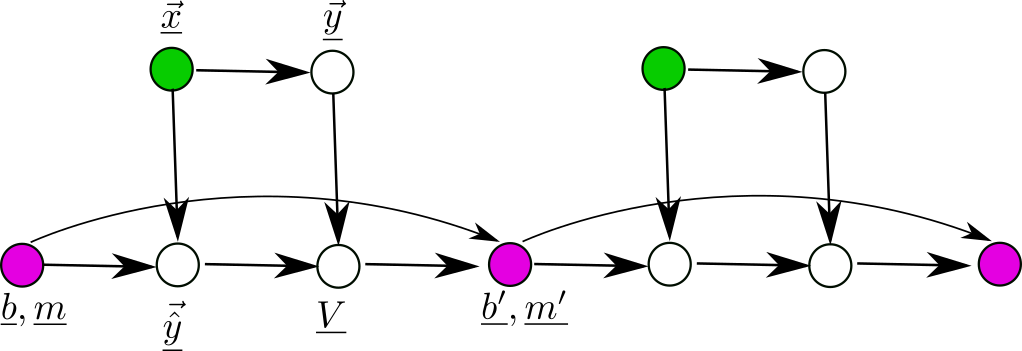
\includegraphics[width=5in]{linreg/linreg.png}
\caption{Linear Regression}
\label{fig-linreg}
\end{figure}

\begin{figure}[h!]
\centering
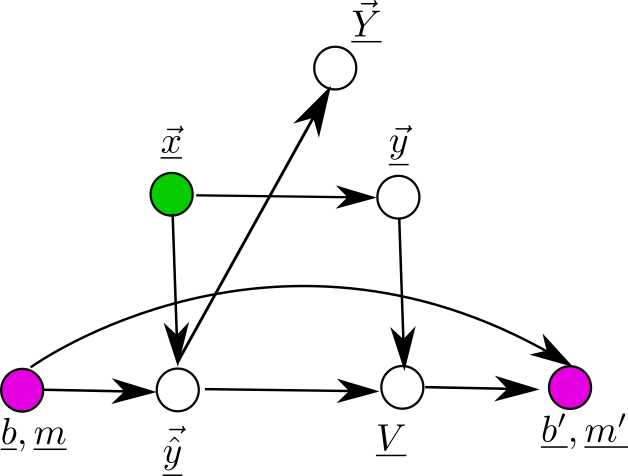
\includegraphics[width=3in]{linreg/linreg-emul.png}
\caption{Bnet of Fig.\ref{fig-linreg}  with new $\vec{\ul{Y}}$ node.}\label{fig-linreg-emul}
\end{figure}



Estimators $\haty$ for linear and logistic regression.
\begin{itemize}
\item

\textbf{Linear Regression:} $y\in \RR$.
Note $\haty\in \RR$. $(x,\haty(x))$ is
the graph
of a straight line
with y-intercept $b$ and slope $m$.
\beq
\haty(x;b, m)= b + mx
\eeq

\item
\textbf{Logistic Regression:} $y\in\{0, 1\}$. Note $\haty\in [0,1]$. $
(x,\haty(x))$ is the graph
of a sigmoid.
 Often in literature, $b,m$ are replaced by $\beta_0, \beta_1$.
\beq
\haty(x;b, m)=\smoid(b + m x)
\eeq
\end{itemize}

Define
\beq
V(b, m)=\sum_{x,y}P(x,y)| y-\haty(x;b, m)|^2
\;.\label{eq-norm-cost}
\eeq
We want to minimize $V(b,m)$ (called a cost or loss function) wrt $b$ and $m$.


The TPMs, printed in blue, for the
Bnet Fig.\ref{fig-linreg}, are as follows.

\beq\color{blue}
P(b,m) \text{ = given}
\eeq
The first time it is used,
$(b,m)$ is arbitrary.
After the first time, it is determined
by previous stage.

Let
\beq
P_{\rvx, \rvy}(x,y)=
\frac{1}{nsam(\vecx)}
\sum_\s \indi(x=x^\s, y=y^\s)
\;.
\eeq

\beq\color{blue}
P(\vecx)=\prod_\s P(x^\s)
\eeq

\beq\color{blue}
P(\vecy|\vecx)=\prod_\s P(y^\s\cond x^\s)
\eeq

\beq\color{blue}
P(\vec{\haty}|\vecx, b, m)=\prod_\s \delta(\haty^\s, \haty(x^\s,b,m))
\label{eq-replace1}
\eeq

\beq\color{blue}
P(V|\vec{\haty}, \vecy)=
\delta(V, \frac{1}{nsam(\vecx)}\sum_\s |y^\s-\haty^\s|^2)
\label{eq-replace2}
\eeq
Let $\eta_b, \eta_m>0$.
For $x=b,m$, if
$x'-x=\Delta x =
-\eta\frac{\partial V}{\partial x}$,
 then $\Delta V\approx
 \frac{-1}{\eta}(\Delta x)^2   \leq 0$
 for $\eta>0$. This is called \enquote{gradient descent}.
\beq\color{blue}
P(b'|V, b)=\delta(b', b-\eta_b\partial_b V)
\eeq
\beq\color{blue}
P(m'|V, m)=\delta(m', m-\eta_m\partial_m V)
\eeq


\section{Generalization to
$x$ with multiple
components (features)}

 Suppose that for each sample $\s$,
instead of $x^\s$ being a scalar,
it has $n$ components called features:

 \beq
x^\s = (x_0^\s, x_1^\s, x_2^\s , \ldots x_{n-1}^\s)
\;.\eeq

Slope $m$ is replaced by weights

\beq
w = (w_0, w_1, w_3, , \ldots, w_{n-1})
\;,\eeq
and the product of 2  scalars $mx^\s$ is replaced by the inner vector product $w^Tx^\s$.

\section{Alternative $V(b,m)$
 for logistic regression}

For logistic regression, since $y^\s\in \{0,1\}$
 and $\haty^\s\in [0,1]$ are both
in the interval $[0,1]$, they can
be interpreted as probabilities. Define
probability distributions $p^\s(x)$ and
$\HAT{p}^\s(x)$ for $x\in \{0,1\}$ by
\beq
p^\s(1)=y^\s,\;\;\; p^\s(0)=1-y^\s
\eeq

\beq
\HAT{p}^\s(1)=\haty^\s,\;\;\; \HAT{p}^\s(0)=1-\haty^\s
\eeq
Then for logistic regression, the following 2 cost functions $V(b,m)$
can be used as alternatives to the cost function Eq.(\ref{eq-norm-cost}) previously given.

\beq
V(b, m)= \frac{1}{nsam(\vecx)}\sum_\s
 D_{KL}(p^\s\parallel \HAT{p}^\s)
\eeq

and

\beqa
V(b, m)&=&\frac{1}{nsam(\vecx)} \sum_\s
CE(p^\s\parallel\HAT{p}^\s)\\
&=& \frac{-1}{nsam(\vecx)}\sum_\s \left\{
y^\s\ln \haty^\s +
(1-y^\s)\ln (1- \haty^\s)\right\}\\
&=&
\frac{-1}{nsam(\vecx)}\sum_\s
\ln \left\{(\haty^\s)^{y^\s}
(1- \haty^\s)^{(1-y^\s)}\right\}\\
&=&
\frac{-1}{nsam(\vecx)}\sum_\s
\ln P(\ul{Y}=y^\s\cond \haty=\haty^\s)\\
&=&
-\sum_{x,y} P(x, y)
\ln P(\ul{Y}=y|\haty=\haty(x,b,m))
\eeqa

Above, we used
\beq
P(\ul{Y}=Y|\haty) = \haty^{Y}
[1-\haty]^{1-Y}
\eeq
for $Y\in S_{\ul{Y}}=\{0,1\}$. (Bernoulli distribution).

There is no node corresponding to $\ul{Y}$
in the Bnet of Fig.\ref{fig-linreg}.
Fig.\ref{fig-linreg-emul} shows a new Bnet
that has a new node called $\vec{\ul{Y}}$
compared to the Bnet of Fig.\ref{fig-linreg}.
One defines the TPMs
for all nodes of Fig.\ref{fig-linreg-emul}
except $\vec{\ul{Y}}$ and $\ul{V}$ the same
as for Fig.\ref{fig-linreg}. For $\vec{\ul{Y}}$
and $\ul{V}$, one defines

\beq\color{blue}
P(Y^\s\cond \vec{\haty})=
P(\ul{Y}=Y^\s\cond \haty^\s)
\eeq

\beq\color{blue}
P(V|\vec{Y}, \vecy)=
\delta(V, \frac{-1}{nsam(\vec{x})}\ln  L)
\;,
\eeq
where $ L =\prod_\s P(\ul{Y}=y^\s\cond \haty^\s )$=likelihood.

\chapter{Linear Systems with Exogenous 
Noise}

In this chapter, we will consider 
bnets which were referred to,
prior to the invention of bnets, as:
Sewall Wright's Path Analysis (PA) and
linear Structural Equations Model (SEM).
Judea Pearl in his
books calls them
linear Structural Causal Models (SCM),
because they are very 
convenient for doing causal analysis.
We will follow 
Judea's convention
and refer to them as scum.


To 
build a SCM,
start with a deterministic bnet $G$.
Now  
add to each node $\rva$ of $G$ a 
root node $\rvU_\rva$
pointing into $\rva$ only.
The nodes $\rvU_\rva$ are called
the {\bf exogenous (external) variables}.
The exogenous
variables make their children noisy.
Their TPMs are
priors and are assumed 
to be unobserved.
Of course, by the
fact that they are 
root nodes, they are assumed 
to be mutually independent.

Examples:
\hrule


\begin{figure}[h!]
$$\xymatrix{
&\rvx\ar[dl]_\beta\ar[dr]^\alp
\\
\rvw\ar[dr]_\epsilon&&\rvz\ar[ll]_\gamma\ar[dl]^\delta
\\
&\rvy
}$$
\caption{}
\label{fig-scm-diamond}
\end{figure}

\beq\color{blue}
P(y|w, z, U_\rvy)=
\indi(y=\epsilon w +\delta z
+ U_\rvy)
\eeq

\beq\color{blue}
P(w|x, z, U_\rvw)=
\indi(w=\beta x +\gamma z + U_\rvw)
\eeq

\beq\color{blue}
P(z|x, U_\rvz)=
\indi(z=\alpha x + U_\rvz)
\eeq

\beq\color{blue}
P(x|U_\rvx)=
\indi(x=U_\rvx)
\eeq

\beqa
y&=&
\epsilon w +\delta z
+ U_\rvy
\\
&=&
\epsilon (\beta x +\gamma z + U_\rvw)
 +\delta z
+ U_\rvy
\\
&=&
(\epsilon\gamma + \delta)z
+ \epsilon\beta x
+\epsilon U_\rvw U_\rvy
\\
&=&
(\epsilon\gamma + \delta)z
+ \epsilon\beta U_\rvx
+\epsilon U_\rvw U_\rvy
\eeqa

\beq
\left(\pder{y}{z}\right)_{U.}=
\epsilon\gamma + \delta
\eeq
sum of terms,
each of those terms
represents a different
causal (not blocked)
path from $\rvz$ to $\rvy(\rvz)$.


\hrule
bnet
with 
deterministic nodes
$\rvx.=(\rvx_k)_{k=0, 1, \ldots nx-1}$
and 
corresponding exogenous nodes 
$\rvU.=(\rvU_k)_{k=0, 1, \ldots nx-1}$.
Assume $\av{\rvU_i, \rvU_j}=0$
if $i\neq j$. The {\bf structural
coefficient} $\alp_{j|i}> 0$
measures the strength of
the connection 
$\rvx_i\rarrow \rvx_j$.
$\av{\rvx, \rvy}$ notation,
for 
covariances 
of any two random variables $\rvx, \rvy$
is explained in the 
Notational
Conventions chapter \ref{ch-not-cons}.

\begin{itemize}

\item {\bf Fully connected graph with $nx=2$}

\begin{figure}[h!]
$$
\xymatrix{
\rvx_0
\ar[d]^{\alp{1|0}}
\\
\rvx_1
}$$
\caption{
Fully connected graph with 2 $\rvx_j$
(exogenous nodes $\rvU_j$
not shown).}
\label{fig-fully-conn-2}
\end{figure}

\begin{subequations}
\label{eq-fully-conn-2}
\beqa
\rvx_0&=&\rvU_0
\\
\rvx_1&=&\alp_{1|0}\rvx_0  + \rvU_1
\eeqa
\end{subequations}
Eqs.\ref{eq-fully-conn-2}
constitute a system of 2 
linear equations in 2 unknowns
(the $\rvx$'s) so can solve
for the $\rvx$'s in terms 
of the $\alpha$'s and $\rvU$'s.


\beq
\av{\rvx_1, \rvx_0}=
\alp_{1|0}\av{\rvx_0, \rvx_0}
\eeq
Thus, $\alp_{1|0}$
can be estimated  
from the covariances $\av{\rvx_i, \rvx_j}$.

\item {\bf Fully connected graph with $nx=3$}

\begin{figure}[h!]
$$
\xymatrix{
\rvx_0\ar[d]_{\alp_{1|0}}
\ar[dr]^{\alp_{2|0}}
\\
\rvx_1\ar[r]^{\alp_{2|1}}
&\rvx_2
}$$
\caption{
Fully connected graph with 3 $\rvx_j$
(exogenous nodes $\rvU_j$
not shown).}
\label{fig-fully-conn-3}
\end{figure}


\begin{subequations}
\label{eq-fully-conn-3}
\beqa
\rvx_0 &=& \rvU_0
\\
\rvx_1&=&\alp_{1|0}\rvx_0 + \rvU_1
\\
\rvx_2&=&\alp_{2|1}\rvx_1 +
\alp_{2|0}\rvx_0 +\rvU_2
\eeqa
\end{subequations}
Eqs.\ref{eq-fully-conn-3}
constitute a system of
3 linear  equations in 3 unknowns
(the $\rvx$'s) so can solve
for the $\rvx$'s in terms 
of the $\alpha$'s and $\rvU$'s.


\begin{subequations}
\label{eq-fully-conn-3-covs}
\beqa
\av{\rvx_1, \rvx_0}&=&
\alp_{1|0}\av{\rvx_0, \rvx_0}
\\
\av{\rvx_2, \rvx_0}&=&
\alp_{2|1}\av{\rvx_1, \rvx_0}
+
\alp_{2|0}\av{\rvx_0, \rvx_0}
\\
\av{\rvx_2, \rvx_1}&=&
\alp_{2|1}\av{\rvx_1, \rvx_1}
+
\alp_{2|0}\av{\rvx_0, \rvx_1}
\eeqa
\end{subequations}
Eqs.\ref{eq-fully-conn-3-covs}
constitute a system of
3 linear  equations in 3 unknowns
(the $\alpha$'s) so can solve
solve for the $\alpha$'s in terms
of covariances $\av{\rvx_i, \rvx_j}$.
This gives an estimate
for the $\alp$'s. 

\end{itemize}
\chapter{Markov Blankets}\label{ch-mblanket}


This chapter is based on the
Wikipedia article, 
Ref.\cite{wiki-mblanket}.
Markov blankets
and Markov boundaries of bnets
were apparently invented
by Judea Pearl. His 1988 book
 Ref.\cite{pearl-1988book},
instead of a research paper, is 
usually given as the original reference.

\begin{figure}[h!]
\centering
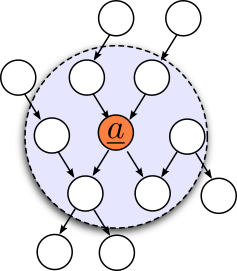
\includegraphics[width=1.5in]{mblanket/mblanket.png}
\caption{In a bnet,
the minimal Markov blanket,
aka Markov boundary,
of node $\rva$.} 
\label{fig-mblanket}
\end{figure}

We will treat vectors 
of random variables as if
they were sets when using the $\in$,
$\subset$ and $-$ operations.
For example,
if $\rvx=(\rvx_0, 
\rvx_1, \rvx_2,
\rvx_3)$ and
$\rvb=(\rvx_1, \rvx_2)$,
then $\rvx_1\in \rvb\subset \rvx$ and
$\rvx-\rvb=(\rvx_0, \rvx_3)$.

Below, $H(\rva:\rvb|\rvc)$
denotes the conditional
mutual information of
random variables
$\rva$ and $\rvb$
conditioned on 
random variable $\rvc$.
$H(\rva:\rvb|\rvc)$
is used in Shannon Information
Theory, where it is defined by

\beq
H(\rva:\rvb|\rvc)=
\sum_{a,b,c}
P(a,b,c)\ln 
\frac{P(a,b|c)}{P(a|c)P(b|c)}
\;.
\eeq
$H(\rva:\rvb|\rvc)=0$
iff $\rva$ and $\rvb$
are independent (uncorrelated)
when $\rvc$ is held fixed.



Suppose
$\rva\in  \rvX$,
 $\rvB\subset \rvX$,
but $\rva\notin\rvB$.
Then $\rvB$ is a Markov blanket
of $\rva$ if

\beq
H(\rva: \rvX-\rva|\rvB)=0
\;.
\eeq
In other words, one may assume that
$\rva$ depends on $\rvB$ only, 
and is independent of all random
variables in $\rvX-(\rva\cup\rvB)$.

The minimal Markov blanket 
is called the Markov boundary.

In a bnet, the Markov boundary
of a node $\rva$,
contains:
\begin{enumerate}
\item
the parents of $\rva$,
\item
the children of $\rva$,
\item
the parents, other than $\rva$,
of the children of $\rva$.
\end{enumerate}
This is illustrated in 
Fig.\ref{fig-mblanket}.
\chapter{Markov Chain Monte Carlo (MCMC)}


Monte Carlo methods
are methods for using
 random number generation to
sample probability distributions.
The subject of Monte Carlo methods
has many branches, as you can see 
from its Wikipedia
category list, Ref.\cite{wiki-monte-carlo}.
MCMC (Markov
Chain Monte Carlo) is just one of those
branches, albeit a major one.
Metropolis-Hastings (MH) sampling
is a very important MCMC method.
Gibbs sampling is
a special case
of MH sampling.
This chapter covers both, MH and Gibbs sampling.
It also covers a few 
other types of sampling.


\section*{Inverse Cumulative Sampling}
For more info about this topic 
and some original references, 
see Ref.\cite{wiki-inv-cum}.

This
is one of the simplest
methods for obtaining
samples from a probability 
distribution $P_\rvx$,
but it
requires knowledge
of the inverse
 cumulative distribution
of $P_\rvx$, which
is often not available.

The {\bf cumulative
distribution} function
is defined by:

\beq
CUM_\rvx(x)=P(\rvx<x)=
\int_{x'<x} dx'\;P_\rvx(x')
\;.
\eeq
Note that

\beq
P_\rvx(x)=\frac{d}{dx}CUM_\rvx(x)
\;.
\eeq


\begin{figure}[h!]
$$\xymatrix{
\rvu^{(0)}\ar[d]
&\rvu^{(1)}\ar[d]
&\rvu^{(2)}\ar[d]
\\
\ul{\vecx}^{(0)}\ar[r]
&\ul{\vecx}^{(1)}\ar[r]
&\ul{\vecx}^{(2)}
}$$
\caption{bnet for Inverse Cumulative Sampling}
\label{fig-mcmc-inverse-bnet}
\end{figure}

For $t=0, 1, \ldots, T-1$, let

$\rvu^{(t)}\in [0,1]$= random variable, 
uniformly
distributed over $[0,1]$.

$\ul{\vecx}^{(t)}=[\rvx^{(t)}_i]_{i=0,1, nsam(t)-1}$
where $\rvx^{(t)}_i \in S_\rvx$ for all $i$. 
Vector of samples collected 
up to time $t$.

The transition prob matrices, printed
in blue, for  the nodes of bnet
 Fig.\ref{fig-mcmc-inverse-bnet}, are:

\beq\color{blue}
P(u^{(t)})=1
\eeq

\beq\color{blue}
P(\vecx^{(t)}|\vecx^{(t-1)}, u^{(t)})=
\indi(\;\;\;\vecx^{(t)}=
[\vecx^{(t-1)}, CUM^{-1}_\rvx(u^{(t)})]
\;\;\;)
\eeq

\hrule\noindent
{\bf Motivation}

\begin{figure}[h!]
\centering
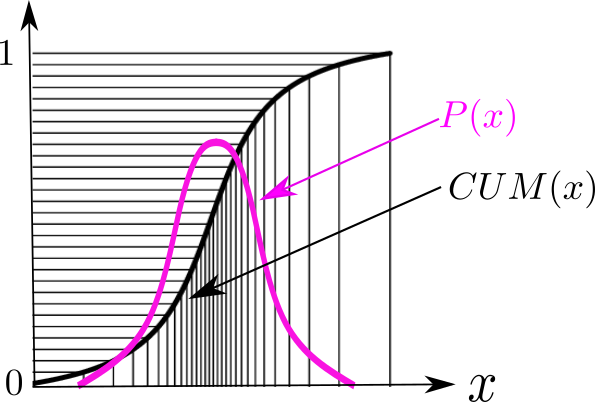
\includegraphics[width=3in]
{mcmc/inverse.png}
\caption{Motivation 
for Inverse of Cumulative Sampling.} 
\label{fig-mcmc-inverse}
\end{figure}
See Fig.\ref{fig-mcmc-inverse}.


Note that if 
$\rvu$ is uniformly distributed over 
the interval $[0,1]$ and $a\in[0,1]$, then

\beq
P(\rvu<a)=a
\;.
\eeq
Thus

\beqa
P(CUM^{-1}_\rvx(\rvu)<x)
&=&P(\rvu<CUM_\rvx(x))
\\
&=&CUM_\rvx(x)
\;.
\eeqa
Therefore,

\beq
P_\rvx(x)dx=dP(CUM^{-1}_\rvx(\rvu)<x)
\;.
\eeq


\section*{Rejection Sampling}

For more info about this topic 
and some original references, 
see Ref.\cite{wiki-reject}.


\begin{figure}[h!]
$$\xymatrix{
&\rvu^{(0)}\ar[d]
&&\rvu^{(1)}\ar[d]
&&\rvu^{(2)}\ar[d]
\\
\ul{\vecx}^{(0)}\ar@/^1pc/[rr]
&\rva^{(0)}\ar[r]
&
\ul{\vecx}^{(1)}\ar@/^1pc/[rr]
&\rva^{(1)}\ar[r]
&
\ul{\vecx}^{(2)}\ar@/^1pc/[rr]
&\rva^{(2)}\ar[r]
&\ul{\vecx}^{(3)}
\\
&\rvc^{(0)}\ar[u]\ar[ru]
&&\rvc^{(1)}\ar[u]\ar[ru]
&&\rvc^{(2)}\ar[u]\ar[ru]
}$$
\caption{bnet for Rejection Sampling}
\label{fig-mcmc-reject-bnet}
\end{figure}

For $t=0, 1, \ldots, T-1$, let

$\rvu^{(t)}\in [0,1]$= random variable, 
uniformly
distributed over $[0,1]$.

$\rva^{(t)}\in \bool$= accept candidate? (no=0, yes=1)

$\rvc^{(t)}\in S_\rvx$=  sample that is a 
candidate for being accepted

$\ul{\vecx}^{(t)}=
[\rvx^{(t)}_i]_{i=0,1, nsam(t)-1}$
where $\rvx^{(t)}_i \in S_\rvx$ for all $i$. 
Vector of samples collected 
up to time $t$.

Assume that
\beq
P_\rvx(x)< \beta P_\rvx(x)
\eeq
for all $x\in S_\rvx$ and some $\beta\in \RR$.

The transition prob matrices, printed
in blue, for  the nodes of bnet
 Fig.\ref{fig-mcmc-reject-bnet}, are:


\beq\color{blue}
P(u^{(t)}=u)=1
\eeq

\beq\color{blue}
P(\rvc^{(t)}=c)=P_\rvx(c)
\eeq

\beq\color{blue}
P(\rva^{(t)}=a|\rvc^{(t)}=c,
\rvu^{(t)}=u)=
\left\{
\begin{array}{ll}
\delta(a, 0)&\text{ if }
u \beta P_\rvx(c)\geq P_\rvx(c))
\\
\delta(a, 1)&\text{ if }
u \beta P_\rvx(c)< P_\rvx(c))
\end{array}
\right.
\eeq

\beq\color{blue}
P(\vecx^{(t)}|
\vecx^{(t-1)}, \rva^{(t)}=a, \rvc^{(t)}=c)
=
\left\{
\begin{array}{ll}
\delta(\vecx^{(t)}, \vecx^{(t-1)})
& \text{ if $a=0$}
\\
\delta(\vecx^{(t)}, [\vecx^{(t-1)}, c])
&\text{ if $a=1$}
\end{array}
\right.
\eeq

\hrule\noindent
{\bf Motivation}

\begin{figure}[h!]
\centering
\includegraphics[width=3.5in]
{mcmc/reject.png}
\caption{Motivation 
for Rejection Sampling.} 
\label{fig-mcmc-reject}
\end{figure}
See Fig.\ref{fig-mcmc-reject}.

\section*{Metropolis-Hastings Sampling}

For more info about this topic and 
some original references, 
see Refs.\cite{bendel-metro-hast}
and \cite{wiki-metro-hast}.

A very convenient
feature of this method is that it can sample
unnormalized probability distributions
$(constant)P_\rvx$ 
because it 
only uses ratios of
$P_\rvx$ at two different points.



\begin{figure}[h!]
$$\xymatrix{
&\rvu^{(0)}\ar[d]
&&\rvu^{(1)}\ar[d]
&&\rvu^{(2)}\ar[d]
\\
\ul{\vecx}^{(0)}\ar@/^1pc/[rr]
&\rva^{(0)}\ar[r]
&
\ul{\vecx}^{(1)}\ar@/^1pc/[rr]\ar[rdd]
&\rva^{(1)}\ar[r]
&
\ul{\vecx}^{(2)}\ar@/^1pc/[rr]\ar[rdd]
&\rva^{(2)}\ar[r]
&\ul{\vecx}^{(3)}
\\
&\rvc^{(0)}\ar[u]\ar[ru]
&&\rvc^{(1)}\ar[u]\ar[ru]
&&\rvc^{(2)}\ar[u]\ar[ru]
\\
&\rvm^{(0)}\ar[u]\ar@/^1pc/[uu]
&&\rvm^{(1)}\ar[u]\ar@/^1pc/[uu]
&&\rvm^{(2)}\ar[u]\ar@/^1pc/[uu]
}$$
\caption{bnet for Metropolis-Hastings Sampling}
\label{fig-mcmc-metro-bnet}
\end{figure}

For $t=0, 1, \dots, T-1$, let

$\rvu^{(t)}\in [0,1]$= random variable,
uniformly
distributed over $[0,1]$.

$\rva^{(t)}\in \bool$= accept candidate? (no=0, yes=1)

$\rvc^{(t)}\in S_\rvx$= sample that is a 
candidate for being accepted

$\rvm^{(t)}\in S_\rvx$= memory
of last accepted sample

$\ul{\vecx}^{(t)}=[\rvx^{(t)}_i]_{i=0,1, nsam(t)-1}$
where $\rvx^{(t)}_i \in S_\rvx$ for all $i$. 
Vector of samples collected 
up to time $t$.

A {\bf proposal transition prob matrix} 
$P_{\rvc|\rvx}:S_\rvx^2\rarrow [0,1]$ 
must be specified a priori 
for this algorithm.

The transition prob matrices, printed
in blue, for  the nodes of bnet
 Fig.\ref{fig-mcmc-metro-bnet}, are:

\beq\color{blue}
P(u^{(t)}=u)=1
\eeq

\beq\color{blue}
P(\rvc^{(t)}=c|m^{(t)}=m)=P_{\rvc|\rvx}(c|m)
\eeq

\beq\color{blue}
P(\rva^{(t)}=a|\rvc^{(t)}=c,
\rvu^{(t)}=u,m^{(t)}=m)=
\left\{
\begin{array}{ll}
\delta(a, 0)&\text{ if }
u \geq \alp(c|m)
\\
\delta(a, 1)&\text{ if }
u < \alp(c|m)
\end{array}
\right.
\eeq
where the 
{\bf acceptance probability}
 $\alp$ is defined as

\beq
\alp(c|m)=\min\left(1,
\frac
{P_{\rvc|\rvx}(m|c)P_\rvx(c)} 
{P_{\rvc|\rvx}(c|m)P_\rvx(m)}
\right)
\;.
\eeq
Note that if the proposal distribution
is symmetric, then

\beq
\alp(c|m)=\min\left(1,
\frac
{P_\rvx(c)} 
{P_\rvx(m)}
\right)
\;.
\eeq

\beq\color{blue}
P(\vecx^{(t)}|
\vecx^{(t-1)}, \rva^{(t)}=a, \rvc^{(t)}=c)
=
\left\{
\begin{array}{ll}
\delta(\vecx^{(t)}, \vecx^{(t-1)})
& \text{ if $a=0$}
\\
\delta(\vecx^{(t)}, [\vecx^{(t-1)}, c])
&\text{ if $a=1$}
\end{array}
\right.
\eeq

\beq\color{blue}
P(\rvm^{(t)}=m|
\vecx^{(t)})=
\delta(m, \text{last component of }
\vecx^{(t)}
)
\eeq

\hrule\noindent
{\bf Motivation}

\begin{figure}[h!]
\centering
\includegraphics[width=3.5in]
{mcmc/metro-hast.png}
\caption{Motivation 
for Metropolis-Hastings Sampling.} 
\label{fig-metro-hast}
\end{figure}
See Fig.\ref{fig-metro-hast}.


Consider a time homogeneous (its
transition
matrix is the same for all times)
Markov chain with
transition prob $P(x'|x)=[T]_{x', x}$.
It's {\bf stationary distribution}, 
if it exists, is
defined as 

\beq 
\pi=\lim_{n\rarrow\infty}T^n\pi_0
\;.
\eeq

Suppose the prob distribution $P_\rvx(x)$
that we wish to sample from
satisfies

\beq
P_\rvx(x)=\pi(x)
\;.
\eeq

{\bf Reversibility (detailed balance):}
\beq
P(x'|x)\pi(x)=P(x|x')\pi(x')
\;.
\eeq
Detailed balance
is a sufficient (although not
necessary) condition
for the stationary 
distribution $\pi$ to exist.

Let
\beq
P(x'|x)=
P(a=1|x',x)P_{\rvc|\rvx}(x'|x)
+\delta(x,x')P(a=0|x)
\;,
\eeq
where

\beq
P(a=0|x)=\sum_{x'} P(a=0|x',x)P_{\rvc|\rvx}(x'|x)
\;.
\eeq

\begin{claim}
If

\beq
P(a=1|x',x)=\alpha(x'|x)
\;,
\eeq
then detailed balance is satisfied.
\end{claim}
\proof
Assume $x\neq x'$.

\beqa
P(x'|x)P(x)&=&
P(a=1|x',x)P_{\rvc|\rvx}(x'|x)P_\rvx(x)
\\
&=&
\min\left(1,
\frac
{P_{\rvc|\rvx}(x|x')P_\rvx(x')} 
{P_{\rvc|\rvx}(x'|x)P_\rvx(x)}
\right)
P_{\rvc|\rvx}(x'|x)P_\rvx(x)
\\
&=&
\min\left(P_{\rvc|\rvx}(x'|x)P_\rvx(x),
{P_{\rvc|\rvx}(x|x')P_\rvx(x')} 
\right)
\\
&=&
P(x|x')P(x')
\eeqa
\qed


\section*{Gibbs Sampling}
For more info about this topic and some 
original references, 
see Ref.\cite{wiki-gibbs-sam}.

Gibbs sampling is a special case
of Metropolis-Hastings sampling.
Gibbs
 sampling is ideally 
suited for application
to a bnet, because
it is stated in
terms of the conditional 
prob distributions
of $N$ random variables,
and conditional 
prob distributions are part of
the definition of a bnet.

Consider a bnet with
nodes $\rvx_0, \rvx_1, \ldots, \rvx_{N-1}$

Identify
the random
variable  $\rvx=(\rvx_0, \rvx_1, \ldots, \rvx_{N-1})$
with the
random variable  $\rvx$ used in 
Metropolis-Hastings sampling.
For Gibbs sampling,
we use the following proposal function:

\beq
P_{\rvc|\rvx}(c|m)=
\prod_{j=0}^{N-1}
P(c_j\cond [m_i]_{i\neq j})
\;.
\label{eq-gibbs-proposal}
\eeq
Eq.(\ref{eq-gibbs-proposal})
can be simplified using 
Markov Blankets
 (see Chapter \ref{ch-mblanket})
to the following:

\beq
P_{\rvc|\rvx}(c|m)=
\prod_{j=0}^{N-1}
P(c_j\cond[m_i: \forall i \ni\rvm_i\in MB(\rvc_j)])
\;,
\eeq
where for any node $\rva$,
we denote its Markov blanket by $MB(\rva)$.


\section*{Importance Sampling}

For more info about this topic and some 
original references, 
see Ref.\cite{wiki-imp-sam}.

Suppose random
variables $\rvx[s]$ for
$s=0, 1, \ldots nsam-1$ are i.i.d.
with probability distribution$P_\rvx$. Then
\beq
E_{\rvx}[f(x)]\approx 
\frac{1}{nsam}\sum_{s=0}^{nsam-1}
f(x[s])
\;.
\eeq
Sometimes,
instead of using i.i.d.
samples $x[s]\sim P_\rvx$,
we wish to use i.i.d. samples
$y[s]\sim P_\rvy$,
where both $\rvx[s]\in S_\rvx$
and $\rvy[s]\in S_\rvx$.


\beqa
E_\rvx[f(\rvx)]
&=&
\sum_x P_\rvx(x)f(x)
\\&=&
\sum_x P_\rvy(x))\frac{P_\rvx(x)}{P_\rvy(x)}f(x
\\&=&
E_{\rvy}[
\frac{P_\rvx(y)}{P_\rvy(y)}f(y)
]
\eeqa

Sampling from $P_\rvy(y)$ instead
of $P_\rvx(x)$
might reduce (or increase) 
variance for a particular
 $f:S_\rvx\rarrow \RR$.

\beq
Var_\rvx[f(x)]=
E_\rvx[(f(x))^2]-(E_\rvx[f(x)])^2
\eeq

\beqa
Var_\rvy[\frac{P_\rvx(y)}{P_\rvy(y)}f(y)]&=&
E_\rvy[(\frac{P_\rvx(y)}{P_\rvy(y)}f(y))^2]-
(E_\rvy[\frac{P_\rvx(y)}{P_\rvy(y)}f(y)])^2
\\
&=&
E_\rvx[\frac{P_\rvx(x)}{P_\rvy(x)}(f(x))^2]-
(E_\rvx[f(x)])^2
\eeqa





\chapter{Markov Chains}

A Markov Chain is simply
a bnet with the graph structure 
of a chain. For example,
Fig.\ref{fig-mchain}
shows a chain with $n=4$ nodes.

\begin{figure}[h!]
\centering
$$\xymatrix{
\rvx_0\ar[r]
&\rvx_1\ar[r]
&\rvx_2\ar[r]
&\rvx_3
}$$
\caption{Markov chain with $n=4$ nodes.}
\label{fig-mchain}
\end{figure}

Because of its
 graph structure,
the TPM of each node
only depends on the state of the previous 
node:

\beq
P(x_t|(x_a)_{a\neq t})=P(x_t|x_{t-1})
\;,
\eeq
where $(x_a)_{a\neq t}$ are all
 the nodes except $x_t$ itself and
$t=1, 2, \dots, n-1$.

If there
exists a single
TPM $P_{\rvx_1|\rvx_0}$
such that

\beq
P(x_t|x_{t-1})=P_{\rvx_1|\rvx_0}
(x_t|x_{t-1})
\;
\eeq
for $t=1, 2,\dots, n-1$, 
then
we say 
that the Markov chain
is {\bf time homogeneous}.
\chapter{Mediation Analysis}
\label{ch-mediation}
This chapter is mostly based on 
Ref.\cite{pearl-2019review}, a 2019
 review of causality by Pearl.

To fully
understand this chapter,
the reader should first read Chapter \ref{ch-counterf}
where do and imagine operators are defined.


\begin{figure}[h!]
$$
\begin{array}{ccc}
\\
\xymatrix{
\rvu_\rvd\ar[dd]
&\rvu_\rvm\ar[d]
&\rvu_\rvy\ar[dd]
\\
&\rvm\ar[rd]
\\
\rvd\ar[ru]\ar[rr]&&\rvy
}
&\;\;\;\;&
\xymatrix{
\rvu_\rvd\ar[dd]\ar@/^2pc/@{<-->}[r]
&\rvu\ar[d]\ar@/^2pc/@{<-->}[r]
&\rvu_\rvy\ar[dd]
\\
&\rvm\ar[rd]
\\
\rvd\ar[ru]\ar[rr]&&\rvy
}
\\
\\
G_0&&G
\end{array}
$$
\caption{DEN bnets $G_0$ and $G$
are used to 
discuss mediation analysis.
In graph
$G_0$,
the external
variables are independent,
whereas in graph $G$
they are not.}
\label{fig-mediation-bnets}
\end{figure}

\begin{figure}[h!]
$$
\begin{array}{c}
\xymatrix{
&\rvh
\ar@{-->}[d]
\ar@{-->}[ldd]
\ar@{-->}[rdd]
\\
&\rvm\ar[rd]
\\
\rvd\ar[ru]\ar[rr]&&\rvy
}
\\
\\
G_{gen}
\end{array}
$$
\caption{General bnet used to 
discuss mediation analysis.
Node $\rvh$ is a hidden confounder.}
\label{fig-gen-bnet-mediation}
\end{figure}

The term ``mediation analysis" (MA)
refers
to  the analysis by Pearl
of the DEN bnet
$G$
in Fig.\ref{fig-mediation-bnets}.
We will discuss MA in terms
of DEN bnets, just as Pearl does.
However, note that much of 
what we will say applies also to 
the general (i.e., not
necessarily a DEN) bnet $G_{gen}$
show in Fig. \ref{fig-gen-bnet-mediation}.



In the DEN bnet $G$,
node $\rvd$ 
influences node
$\rvy$
both
directly
and via the mediator node $\rvm$.
The structural 
equations for $G$
are of the form:

\begin{subequations}
\label{eq-struc-eqs-med}
\beqa
\rvd&=&\rvu_\rvd
\\
\rvm&=&f_\rvm(\rvd, \rvu_\rvm)
\\
\rvy&=&f_\rvy(\rvd, \rvm, \rvu_\rvy)
\;.
\eeqa
\end{subequations}
Thus,

\beq
\rvy=f_\rvy(u_\rvd, 
f_\rvm(\rvu_\rvd, \rvu_\rvm), \rvu_\rvy)
\;.
\eeq

\begin{figure}[h!]
$$
\begin{array}{cccc}
\\
\xymatrix{
\rvu_\rvd\ar@/^2pc/@{<-->}[r]
&\rvu_\rvm\ar[d]\ar@/^2pc/@{<-->}[r]
&\rvu_\rvy\ar[dd]
\\
&\rvm\ar[rd]
\\
\rvd=5\ar[ru]
\ar[rr]&&\rvy
}
&\;\;\;\;\;&
\xymatrix{
\rvu_\rvd\ar[dd]\ar@/^2pc/@{<-->}[rr]
&&\rvu_\rvm\ar[d]\ar@/^2pc/@{<-->}[r]
&\rvu_\rvy\ar[dd]
\\
&^{\cali_\rvm{\rvd}=5}\ar[r]
&\rvm\ar[rd]
\\
\rvd
\ar[rrr]
&&&\rvy
}
\\
\\
\cald_{\rvd=5}G
&&
\cali_{\rvd\rarrow\rvm}(5)G
\end{array}
$$
\caption{Graph $G$
of Fig.\ref{fig-mediation-bnets}
after applying do operator $\cald_{\rvd=5}$
and imagine operator 
$\cali_{\rvd\rarrow\rvm}(5)$.}
\label{fig-mediation-ops-egs}
\end{figure}

If we apply
$\cald_{\rvd=5}G$
to Eqs.(\ref{eq-struc-eqs-med}), we get

\begin{subequations}
\label{eq-mediation-rho-egs}
\beqa
\rvd&=&5
\\
\rvm&=&f_\rvm(\rvd, \rvu_\rvm)
\\
\rvy&=&f_\rvy(\rvd, \rvm, \rvu_\rvy)
\;.
\eeqa
\end{subequations}
Eqs.\ref{eq-mediation-rho-egs}
are represented graphically
in Fig.\ref{fig-mediation-ops-egs}.
We will often denote the  random variable
 $\rvy$ in Eqs.(\ref{eq-mediation-rho-egs})
by the more explicit symbol 
$\rvy_{\cald_{\rvd=5}G}$.
Pearl often 
refers to
this $\rvy$ by the less explicit symbol
$Y_5$ or $Y_5(u)$ where 
$u=(u_\rvm, u_\rvy)=u_{!\rvd}$.

If we apply
$\cali_{\rvd\rarrow\rvm}(5)G$
to Eqs.(\ref{eq-struc-eqs-med}), we get

\begin{subequations}
\label{eq-mediation-kappa-egs}
\beqa
\rvd&=&\rvu_\rvd
\\
\rvm&=&f_\rvm(5, \rvu_\rvm)
\\
\rvy&=&f_\rvy(\rvd, \rvm, \rvu_\rvy)
\;.
\eeqa
\end{subequations}
Eqs.\ref{eq-mediation-kappa-egs}
are represented graphically
in Fig.\ref{fig-mediation-ops-egs}.
We will often denote the  random variable
 $\rvy$ in Eqs.(\ref{eq-mediation-kappa-egs})
by the more explicit symbol 
$\rvy_{\cali_{\rvd\rarrow\rvm}(5)G}$.
 Pearl often 
refers to
this $\rvy$ by the less explicit symbol
$Y_5$ or $Y_5(u)$ where
$u=(u_\rvd, u_\rvm, u_\rvy)$.

\hrule

\begin{figure}[h!]
$$
\begin{array}{cccc}
\\
\xymatrix{
\rvu_\rvd\ar@/^2pc/@{<-->}[r]
&\rvu_\rvm\ar[d]\ar@/^2pc/@{<-->}[r]
&\rvu_\rvy\ar[dd]
\\
&\rvm\ar[rd]
\\
\rvd=d\ar[ru]
\ar[rr]&&\rvy
}
&\;\;\;\;
&
\xymatrix{
\rvu_\rvd\ar@/^2pc/@{<-->}[r]
&\rvu_\rvm\ar@/^2pc/@{<-->}[r]
&\rvu_\rvy\ar[dd]
\\
&\rvm=m\ar[rd]
\\
\rvd=d
\ar[rr]&&\rvy
}
\\
\\
\cald_{\rvd=d}G
&&
\cald_{\rvd=d}\cald_{\rvm=m}G
\end{array}
$$
\caption{Graph $G$
of Fig.\ref{fig-mediation-bnets}
after applying the 
do operators $\cald_{\rvd=d}$
and
$\cald_{\rvd=d}\cald_{\rvm=m}$.}
\label{fig-mediation-rho}
\end{figure}
Define the Total Effect (TE),
and the
Controlled Direct Effect (CDE) by
\beqa
TE&=& E[
\rvy_{\cald_{\rvd=1}G}
-\rvy_{\cald_{\rvd=0}G}
]
\\
CDE(m)&=&
E[
\rvy_{\cald_{\rvd=1}\cald_{\rvm=m}G}
-\rvy_{\cald_{\rvd=0}\cald_{ \rvm=m}G}
]
\eeqa
The two DEN diagrams
$\cald_{\rvd=d}G$
and
$\cald_{\rvd=d}\cald_{\rvm=m}G$
used in the definitions
of $TE$ and $CDE$
are given in Fig.\ref{fig-mediation-rho}.
\hrule

\begin{figure}[h!]
$$
\begin{array}{c}
\\
\xymatrix{
\rvu_\rvd\ar@/^2pc/@{<-->}[rr]
&&\rvu_\rvm\ar[d]\ar@/^2pc/@{<-->}[r]
&\rvu_\rvy\ar[dd]
\\
&\cali_\rvm\rvd=d'\ar[r]
&\rvm\ar[rd]
\\
\cald \rvd=d\ar[rrr]
&
&&\rvy
}
\\
\\
\cald_{\rvd=d}
\cali_{\rvd\rarrow\rvm}(d')
G
\end{array}
$$
\caption{
Graph $G$
of Fig.\ref{fig-mediation-bnets}
after
applying the 
imagine operator
 $\cali$
 to arrow
$\rvd\rarrow\rvm$ and 
the do operator to node $\rvd$.}
\label{fig-mediation-kappa}
\end{figure}

Let

\beq
\caly_d^{d'}=
 E[
\rvy_{\cald_{\rvd=d}
\cali_{\rvd\rarrow\rvm}(d')
G}
]
\eeq
Fig.\ref{fig-mediation-kappa}
shows the diagram 
$
\cald_{\rvd=d}\cali_{\rvd\rarrow\rvy}(d')G$
used in
the definition of $\caly_d^{d'}$.


Now define the
Natural Direct Effect (NDE), and the
Natural Indirect Effect (NIE)
by
\beqa
NDE
&=&\caly_1^0 - \caly_0^0
\\
NIE(d)
&=&\caly_d^1 - \caly_d^0
\;.
\eeqa

Note that
\beqa
NDE+NIE(1)&=&(\caly_1^0-\caly_0^0)+(\caly_1^1 - \caly_1^0)
\\
&=&\caly_1^1-\caly_0^0
\\
&=&
TE
\;.
\eeqa

$TE$ and the ``controlled effect"
$CDE(m)$
contain do operators
but no imagine 
operators 
so one can do 
intervention 
experiments to
calculate them.
On the other hand,
the ``natural effects" $NDE$ and $NIE(d)$
contain
imagine 
operators
(and therefore
counterfactual
distributions)
so it's not
obvious how to 
calculate them,
or even whether it
is possible to do so.
The next claim
shows how to calculate
$NDE$ in certain
cases. In technical jargon,
the claim 
gives sufficient conditions
for $\cald\cali$-identifiability
of $NDE$. 
If $NDE$ is $\cald\cali$-identifiable,
then $NIE(1)$ is too,
because they add to
$TE$, 
which is identifiable.


\begin{figure}[h!]
$$
\begin{array}{c}
\\
\xymatrix{
\rvu_\rvd\ar@/^2pc/@{<-->}[rr]
&&\rvu_\rvm\ar@/^2pc/@{<-->}[r]
&\rvu_\rvy\ar[dd]
\\
\cald\rvd'=0\ar@/_1.5pc/[rr]
&\ul{\xi}.\ar[r]
&\cald\rvm\ar[rd]
\\
\cald \rvd=d\ar[rrr]
&
&&\rvy
}
\end{array}
$$
\caption{
Bnet alluded to in Claim \ref{cl-adjust-nde}
}
\label{fig-adjust-nde}
\end{figure}


\begin{claim}(Adjustment formula for NDE)
\label{cl-adjust-nde}

Suppose $\xi.$
is a multinode of the bnet.
If 
\begin{enumerate}
\item
 $\ul{\xi}.\cap de(\rvd)=\emptyset$
(i.e., $\ul{\xi}.$ contains no descendants 
of $\rvd$)
\item conditioning on $\ul{\xi}.$ blocks
all backdoor paths from $\rvd$ to $\rvy$,
\end{enumerate}
then  (see Fig.\ref{fig-adjust-nde})
\beq
NDE = \sum_m\sum_{\xi.}[
\caly_1^m(\xi.)-\caly_0^m(\xi.)]
P(m|\cald\rvd=0, \xi.)P(\xi.)
\eeq
where

\beq
\caly_d^m(\xi.)=
E_{|\xi.}[\rvy_{\cald_{\rvd=d},\cald_{\rvm=m}G}]
\;.
\eeq 
If besides 1 and 2, the following are true:
\begin{enumerate}
\item[3.]
$P(m|\cald\rvd=0, \xi.)$
is $\cald$-identifiable (i.e., expressible without do's)
\item[4.]
$\caly_d^m(\xi.)$ is $\cald$-identifiable
\end{enumerate}
then
\beq
NDE = \sum_m\sum_{\xi.}[
\caly_1^m(\xi.)-\caly_0^m(\xi.)]
P(m|\rvd=0, \xi.)P(\xi.)
\eeq
where 
\beq
\caly_d^m(\xi.)=
E_{|d, m, \ul{\xi}.}[\rvy]
\eeq
If besides 1,2,3,4, the following is true

\begin{enumerate}
\item[5.] there is no confounding 
connecting the external nodes $\rvu_\rvd, \rvu_\rvy, \rvu_\rvm$,
\end{enumerate}
then
\beq
NDE = \sum_m[
\caly_1^m-\caly_0^m]
P(m|\rvd=0)
\eeq
where 
\beq
\caly_d^m=
E_{|d, m}[\rvy]
\eeq
\end{claim}
\proof 
See references in Ref.\cite{pearl-2019review}.
\qed


\chapter{Message Passing, Pearl's theory}
\label{ch-mpass}

This chapter is mostly
based on chapter 4 of 
Ref.\cite{pearl-1988book}
by Pearl.
Refs.\cite{wiki-mp},
and \cite{neapolitan2004learning}
were also helpful in writing this chapter.

In his book Ref.\cite{pearl-1988book},
Pearl explains two types 
of Message Passing (i.e., distributed 
computing in a bnet). In Chapter 4, he discusses
one type of MP which he calls Belief Propagation (BP)
or Belief Updating. In Chapter 5, he introduces
a second type of MP which is he calls Belief Revision, but
which I prefer to call
Explanation Optimization (EO).
This chapter will be devoted to BP only.


BP
was first proposed for bnets in 1982
Ref.\cite{pearl1982reverend} by Judea Pearl
to simplify
the exact evaluation of the probability
of one node conditioned 
on other nodes
of a bnet (exact inference).
It gives exact results for trees and
polytrees (i.e., bnets with
a single connected component and
 no
loops). For bnets with loops,
it gives approximate results
(loopy belief propagation),
and it has been generalized to
the junction tree algorithm
(see Chapter \ref{ch-junc-tree})
which can do exact inference
for general bnets with loops.
The basic idea behind
the junction tree algorithm
is to eliminate
loops by clustering
them into single nodes.



\section{Distributed Soldier Counting}
Consider
a group of soldiers marching single file.
Fig.\ref{fig-soldiers}
shows several methods by which 
a member of the group 
can obtain a count 
of the soldiers without
breaking the line to do 
global operations.
This can be done in
a distributed fashion, 
with every soldier doing
only local operations
(i.e.,
each soldier 
can only 
send
messages
to either
the soldier in front
or the one in
back).
Such 
distributed soldier counting is a rudimentary
type of BP.
In the next section,
we will
generalize this BP for soldiers
to BP for a Markov chain.
\newpage


\begin{figure}[h!]
\centering
\includegraphics[width=4in]
{mpass/soldiers.png}
\caption{Distributed soldier counting 
(This example
comes from Chapter 4 of
Ref.\cite{pearl-1988book}). 
Green dots indicate the
beginning and red dots the end
of a count. Only
first soldier can calculate
total count in (a). Only 
third soldier can calculate total count
in (b,c). 
All soldiers can calculate
the total count in 
(d,e). One starting point
in (a,b,e).
Two ends as starting points
in (c,d).
} 
\label{fig-soldiers}
\end{figure}

\section{Spring Systems}


\begin{figure}[h!]
\centering
\includegraphics[width=3in]
{mpass/spring-net.png}
\caption{Spring system.
Point masses connected by springs.}
\label{fig-sping-net}
\end{figure}

\begin{figure}[h!]
\centering
\includegraphics[width=2.7in]
{mpass/time-travel.png}
\caption{Diagram $(a)$ portrays two events interacting via feedback. Diagram $(b)$
represents the same thing as diagram $(a)$
after \qt{unrolling} it.}
\label{fig-time-travel}
\end{figure}

See Ref.\cite{wiki-spring-net}
for an introduction to spring systems.
Ideal springs between the point mass
nodes would
not be sufficient.
One would have to add damping to
the springs so as
to reach an equilibrium.
Time dependent forces (loads)
pointing into or out of the page, applied
to the point masses, would
generate signals that would
propagate
like BP messages.


The messages in Fig.\ref{fig-time-travel} $(a)$
appear to travel both forward and backwards in time.
But in reality, messages cannot travel backward in time.  Fig.\ref{fig-time-travel} $(a)$
is just a convenient representation of
Fig.\ref{fig-time-travel} $(b)$, which \qt{unrolls} it. Both $(a)$ and $
(b)$ are representations of feedback.
Messages that appear to travel back in time,
(but in reality don't, this are just a convenient
representation of feedback)
is a recurring theme in Physics. For example,
in Quantum Electrodynamics, it appears that positrons can travel backwards in time.  In reality,
they are portraying the feedback mechanism whereby two
charged
particles
apply a force on each other.


\section{BP for Markov Chains}

\hrule
Notation:

$\rva\rdart\rvb$ and $\rvb\ldart\rva$ will mean the same thing, namely either a dot or dashed
message arrow, but not a bnet arrow.

$\pi_{\rvb\ldart\rva}(a) = P(a|\eps^-)$

$\lam_{\rvb\rdart\rva}(b) = P(\eps^+|b)$

Note that the argument of 
$\pi_{\rvb\ldart\rva}(a)$ and
$\lam_{\rvb\rdart\rva}(b)$ is the node at
the starting end of the double arrow.

The $\pi$  messages
(probability functions)
travel downstream (i.e., 
they carry info
in the direction
of the graph arrows, towards the future)
and are indicated by a dashed arrow
or by a left double arrow $\ldart$. 
The $\lam$  messages 
(likelihood functions) travel 
upstream (i.e., they 
carry info opposite to 
direction of the graph arrows,
towards the past)
and are indicated
by a dotted arrow
or by a right double arrow $\rdart$.
$\rveps^+$
stands for future evidence and 
$\rveps^-$ for past evidence. 
\hrule



Note that Bayes rule would affirm
 that\footnote{As usual in this book,
$\caln(!x)$ means
a constant that is independent of $x$.}

\beq
P(x|\eps^+)=
\caln(!x)
\underbrace{P(\eps^+|x)}_
{\lam_{\rveps^+\rdart \rvx}(x)}
P(x)
\;.
\eeq
Thus, Eq.(\ref{eq-2-sided-bayes})
is like a 2-sided Janus Bayes rule.

Note that the $\pi$ messages and
$\lam$ messages propagate 
independently
of each other, via the 
 TPM $P(x|\eps^-)$:

\begin{subequations}
\beq
\underbrace{\pi_{\rveps^+\ldart\rvx}(x)}_
{P(x|\eps^-_0)}
=\sum_{\eps^-}P(x|\eps^-)
\underbrace{\pi_{\rvx\ldart \rveps^-}(\eps^-)}_
{\delta(\eps^-, \eps^-_0)}
\eeq

\beq
\underbrace{
\lam_{\rvx\rdart \rveps^-}(\eps^-)}_
{P(\eps^+|\eps^-)}
=
\sum_x P(x|\eps^-)
\underbrace{
\lam_{\rveps^+\rdart \rvx}(x)}_
{P(\eps^+|x)}
\eeq
\label{eq-pi-lam-propagate}
\end{subequations}

Eqs.(\ref{eq-pi-lam-propagate})
suggest that we define an edge bnet
for the $\pi$ and $\lam$
messages (these messages
live in the edges
between the nodes
$\rveps^+, \rvx, \rveps^-$).
Such an edge bnet, shown
in Fig.\ref{fig-BEL-2pi}, is 
complementary to 
bnet for the nodes themselves.
We will call it
the {\bf BP 2-track bnet}
for the bnet Fig.\ref{fig-mp-3chain},
because it has two \qt{tracks},
one for $\pi$ messages and another
for $\lam$ ones.
The TPMs, printed in blue,
for bnet
Fig.\ref{fig-BEL-2pi}, are 
as follows:

\begin{figure}[h!]
$$\xymatrix{
&\ul{\pi}_{\rveps^+\ldart\rvx}\ar[dr]
&&\ul{\pi}_{\rvx\ldart\rveps^-}\ar[ll]
\\
&&\rvB_\rvx
\\
&\ul{\lam}_{\rveps^+\rdart\rvx}\ar[rr]\ar[ru]
&&\ul{\lam}_{\rvx\rdart\rveps^-}
}$$
\caption{BP 2-track
bnet for the bnet
 Fig.\ref{fig-mp-3chain}.}
\label{fig-BEL-2pi}
\end{figure}


\hrule

\begin{figure}[h!]
$$\xymatrix{
\rveps^+
\ar@{<--}@<2ex>[rr]^{\pi_{\rveps^+\ldart\rvb}}
\ar@{.>}@<-2ex>[rr]_{\lam_{\rveps^+\rdart\rvb}}
&&
\rvb\ar[ll]
\ar@{<--}@<2ex>[rr]^{\pi_{\rvb\ldart\rvx}}
\ar@{.>}@<-2ex>[rr]_{\lam_{\rvb\rdart\rvx}}
&&
\rvx\ar[ll]
\ar@{<--}@<2ex>[rr]^{\pi_{\rvx\ldart\rva}}
\ar@{.>}@<-2ex>[rr]_{\lam_{\rvx\rdart\rva}}
&&
\rva\ar[ll]
\ar@{<--}@<2ex>[rr]^{\pi_{\rva\ldart\rveps^-}}
\ar@{.>}@<-2ex>[rr]_{\lam_{\rva\rdart\rveps^-}}
&&
\rveps^-\ar[ll]
}$$
\caption{5 node Markov chain}
\label{fig-mp-5chain}
\end{figure}

So far in 
this section, we have considered Markov
chains with 3 nodes.
Before 
concluding our
discussion of BP for Markov chains,
let us consider BP
for a slightly longer chain.
Let us consider
the 5 node Markov
chain
$\rveps^+\larrow\rvb\larrow\rvx\larrow\rva\larrow\rveps^-$
shown in Fig.\ref{fig-mp-5chain}.
We have already dealt 
with the end nodes
of a Markov chain in the 
3 node Markov chain
example above,
so in the 
5 node case, let us
focus on the internal (i.e., not at
an end) node $\rvx$ and its neighbors
$\rva$ and $\rvb$. Define



\beq
\begin{array}{l|l|l|l}
\pi_{\rveps^+\ldart \rvb}(b)=
P(b|\eps^-)
&
\pi_{\rvb\ldart \rvx}(x)=
P(x|\eps^-)
&
\pi_{\rvx\ldart \rva}(a)=
P(a|\eps^-)
&
\pi_{\rva\ldart \rveps^-}(\eps^-)=
P(\eps^-|\eps^-)
\\
\lam_{\rveps^+\rdart \rvb}(\eps^+)=
P(\eps^+|\eps^+)
&
\lam_{\rvb\rdart \rvx}(b)=
P(\eps^+|b)
&
\lam_{\rvx\rdart \rva}(x)=
P(\eps^+|x)
&
\lam_{\rva\rdart \rveps^-}(a)=
P(\eps^+|a)
\end{array}
\eeq


In analogy
with the case of BP for a
P(\pi_{\rvb\ldart\rvx}|\pi_{\rvx\ldart\rva})=
\prod_{x}\indi\left(
\pi_{\rvb\ldart\rvx}(x)=\sum_a P(x|a)
\pi_{\rvx\ldart\rva}(a)
 3 node Markov
chain, we can define the bnet
Fig.\ref{fig-BEL-4pi},
which we refer to as the
{\bf BP
2-track bnet} for Fig.\ref{fig-mp-5chain}.
The TPMs, printed in blue,
 for bnet Fig.\ref{fig-BEL-4pi}, are
as follows:





\begin{figure}[h!]
$$\xymatrix{
&\ul{\pi}_{\rveps^+\ldart\rvb}\ar[dr]
&&\ul{\pi}_{\rvb\ldart\rvx}\ar[ll]\ar@[red][dr]
&&\ul{\pi}_{\rvx\ldart\rva}\ar@[red][ll]\ar[dr]
&&\ul{\pi}_{\rva\ldart\rveps^-}\ar[ll]
\\
&&\rvB_\rvb
&&\rvB_\rvx
&&\rvB_\rva
\\
&\ul{\lam}_{\rveps^+\rdart\rvb}\ar[rr]
&&\ul{\lam}_{\rvb\rdart\rvx}
\ar@[red][rr]\ar[ul]
&&\ul{\lam}_{\rvx\rdart\rva}\ar[rr]\ar@[red][ul]
&&\ul{\lam}_{\rva\rdart\rveps^-}\ar[ul]
}$$
\caption{BP 2-track bnet for the bnet
Fig.\ref{fig-mp-5chain}.}
\label{fig-BEL-4pi}
\end{figure}


\beq\color{blue}
P(\pi_{\rvb\ldart\rvx}|\pi_{\rvx\ldart\rva})=
\prod_{x}\indi\left(
\pi_{\rvb\ldart\rvx}(x)=\sum_a P(x|a)
\pi_{\rvx\ldart\rva}(a)
\right)
\label{eq-pr-pi-bar-pi}
\eeq

\beq\color{blue}
P(\lam_{\rvx\rdart \rva}|
\lam_{\rvb\rdart \rvx})=
\prod_{a}
\indi\left(
\lam_{\rvx\rdart \rva}(a)
=
\sum_x P(x|a)
\lam_{\rvb\rdart \rvx}(x)
\right)
\label{eq-pr-lam-bar-lam}
\eeq

\beq\color{blue}
P(B_\rvx|
\pi_{\rvb\ldart \rvx},
\lam_{\rvx\rdart \rva})=
\prod_x
\indi\left(
B_\rvx(x)=BEL_\rvx(x)
\right)
\eeq



Let us represent the Markov
chain of Fig.\ref{fig-mp-5chain}
by
$\rvx_{nx-1}
\larrow \ldots, \rvx_2\larrow \rvx_1\larrow \rvx_0$
where $nx=5$.
For any node 
$\rvx_i$
with
parent $\ul{px}_i=\rvx_{i-1}$
and child $\ul{cx}_i=\rvx_{i+1}$, 
define
the {\bf memory matrix}
$\calm_{\rvx_i}$
for node $\rvx_i$
as

\beq
\calm_{\rvx_i}=
[
\calm^+_{\rvx_i},
\calm^-_{\rvx_i}]
\;,
\eeq
where $+=$future, $-=$past, and 

\beq
\calm^+_{ \rvx_i}=
\left[
\begin{array}{c}
\pi_{\ul{cx}_i\ldart \rvx_i}(\cdot)
\\
\lam_{\ul{cx}_i\rdart \rvx_i}(\cdot)
\end{array}
\right]
\;, 
\;\;\;
\calm^-_{\rvx_i}=
\left[
\begin{array}{c}
\pi_{\rvx_i \ldart \ul{px}_i}(\cdot)
\\
\lam_{\rvx_i \rdart \ul{px}_i}(\cdot)
\end{array}
\right]
\;.
\eeq 
Note that

\beq
\calm^-_{\rvx_i}=
\calm^+_{\ul{px}_i}
\label{eq-mem-overlap}
\eeq
for all nodes $\rvx_i$.
We will refer to
Eqs.(\ref{eq-mem-overlap}) as
the {\bf memory overlap
conditions}.

We will also use a permuted version of the 
memory matrix

\beq
\calm'_{\rvx_i}=
[
\calm^{OUT}_{\rvx_i},
\calm^{IN}_{\rvx_i}]
\;,
\eeq
where

\beq
\calm^{OUT}_{ \rvx_i}=
\left[
\begin{array}{c}
\pi_{\ul{cx}_i\ldart \rvx_i}(\cdot)
\\
\lam_{\rvx_i \rdart \ul{px}_i}(\cdot)
\end{array}
\right]
\;, 
\;\;\;
\calm^{IN}_{\rvx_i}=
\left[
\begin{array}{c}
\pi_{\rvx_i \ldart \ul{px}_i}(\cdot)
\\
\lam_{\ul{cx}_i\rdart \rvx_i}(\cdot)
\end{array}
\right]
\;.
\eeq

\begin{figure}[h!]
$$\xymatrix{
\ucalm_{\rveps^+}
&
\ucalm_\rvb\ar[l]
&
\ucalm_\rvx\ar[l]
&
\ucalm_\rva\ar[l]
&
\calm_{\rveps^-}\ar[l]
}$$
\caption{BP Memory Bnet for the bnet
Fig.\ref{fig-mp-5chain}. }
\label{fig-mem-5chain}
\end{figure}

Unfortunately,
2-track bnets cannot be
 generalized in any
obvious way  from 
Markov chains to more
complicated DAGs.
An alternative to 2-track bnets
that still
carries message
info in its nodes,
are memory bnets. An BP
{\bf memory bnet}
is a bnet 
which takes each node
of an original
bnet and
adds a local memory to it.
More specifically,
it keeps that DAG
but replaces each node
$\rvx_i$
by a memory $\ucalm_{\rvx_i}$.
Fig.\ref{fig-mem-5chain} shows 
the memory bnet for
the bnet Fig.\ref{fig-mp-5chain}.
The TPM, printed in blue,
for the  node $\ucalm_\rvx$
of the memory bnet 
Fig.\ref{fig-mem-5chain}, is as follows

\beq\color{blue}
P(\calm_{\rvx_i}|
\calm_{\rvn\in nb(\rvx_i)}
)= A B
\;,
\eeq
where

\beq
A=
\indi(\calm^{-}_{\rvx_i}=\calm^{+}_{\ul{px}_i})
\;,
\eeq
and

\beq
B=
\indi(\calm^{OUT}_{\rvx_i}=\calc(\calm^{IN}_{\rvx_i}))
\label{eq-mp-update-static}
\;.
\eeq
The function $\calc$,
which 
we will call the {\bf BP local computation},
maps $\calm^{IN}_{\rvx_i}$
into $\calm^{OUT}_{\rvx_i}$. More explicitly,
$\calc$ is defined so that

\beq
B
=
\underbrace{P(\pi_{\rvb\ldart\rvx}|
\pi_{\rvx\ldart\rva})}_{B_\pi}
\underbrace{P(\lam_{\rvx\rdart \rva}|
\lam_{\rvb\rdart \rvx})}_{B_\pi}
\;,
\eeq
where
$B_\pi$ and $B_\lam$
are given by Eqs.(\ref{eq-pr-pi-bar-pi})
and (\ref{eq-pr-lam-bar-lam}),
respectively.



The BP memory bnet
 Fig.
\ref{fig-mem-5chain}
is a deterministic bnet.
A deterministic bnet
is basically
just a coupled system
of equations (CSE)
for some unknowns $x_i$. 
A CSE per se does not
include with it a method for  
solving for the $x_i$. Such methods are not
unique.
For example,
for the 
distributed
soldier counting 
problem,
the various 
methods that
we described
for counting soldiers
are just different
methods 
for solving the same
CSE.
One can describe 
a method for solving a
CSE using a dynamical bnet.\footnote{
The term
dynamical bnet
was used in Chapter \ref{ch-dyn-bnets}
to mean a time inhomogeneous
Markov chain, but 
here we are stretching its meaning to
include
Markov chains
that aren't 
time inhomogeneous.}
To solve
the CSE
represented by
the memory bnet Fig.\ref{fig-mem-5chain},
we will use the 
dynamical bnet
Fig.\ref{fig-propagation-5chain}.
Henceforth, 
we will refer to
Fig.\ref{fig-propagation-5chain} as
an {\bf BP dynamical bnet}
for Fig.\ref{fig-mem-5chain}.

\begin{figure}
$$\xymatrix{
\rveps^-\ar[d]
&\ucalm^{(0)}_{\rveps^-}\ar[r]\ar[dr]
&\ucalm^{(1)}_{\rveps^-}\ar[r]
&\ucalm^{(2)}_{\rveps^-}\ar[r]
&\ucalm^{(3)}_{\rveps^-}\ar[r]
&\ucalm^{(4)}_{\rveps^-}
&
\\
\rva\ar[d]
&\ucalm^{(0)}_{\rva}\ar[r]
&\ucalm^{(1)}_{\rva}\ar[r]\ar[dr]
&\ucalm^{(2)}_{\rva}\ar[r]
&\ucalm^{(3)}_{\rva}\ar[r]\ar[ur]
&\ucalm^{(4)}_{\rva}
\\
\rvx\ar[d]
&\ucalm^{(0)}_{\rvx}\ar[r]
&\ucalm^{(1)}_{\rvx}\ar[r]
&\ucalm^{(2)}_{\rvx}\ar[r]\ar[dr]\ar[ur]
&\ucalm^{(3)}_{\rvx}\ar[r]
&\ucalm^{(4)}_{\rvx}
\\
\rvb\ar[d]
&\ucalm^{(0)}_{\rvb}\ar[r]
&\ucalm^{(1)}_{\rvb}\ar[r]\ar[ur]
&\ucalm^{(2)}_{\rvb}\ar[r]
&\ucalm^{(3)}_{\rvb}\ar[r]\ar[dr]
&\ucalm^{(4)}_{\rvb}
\\
\rveps^+
&\ucalm^{(0)}_{\rveps^+}\ar[r]\ar[ur]
&\ucalm^{(1)}_{\rveps^+}\ar[r]
&\ucalm^{(2)}_{\rveps^+}\ar[r]
&\ucalm^{(3)}_{\rveps^+}\ar[r]
&\ucalm^{(4)}_{\rveps^+}
}$$
\caption{BP dynamical bnet for the bnet
  Fig.\ref{fig-mem-5chain}.}
\label{fig-propagation-5chain}
\end{figure}

\begin{figure}[h!]
$$
\xymatrix{
\rveps^+\ar@[red]@{.>}@<-2ex>[r]
&\rvb\ar[l]
&\rvx\ar[l]
&\rva\ar[l]
&\rveps^-\ar[l]\ar@[red]@{-->}@<-2ex>[l]
\\
\rveps^+
&\rvb\ar[l]\ar@[red]@{.>}@<-2ex>[r]
&\rvx\ar[l]
&\rva\ar[l]\ar@[red]@{-->}@<-2ex>[l]
&\rveps^-\ar[l]
\\
\rveps^+
&\rvb\ar[l]
&\rvx\ar[l]\ar@[red]@{.>}@<-2ex>[r]
\ar@[red]@{-->}@<-2ex>[l]
&\rva\ar[l]
&\rveps^-\ar[l]
\\
\rveps^+
&\rvb\ar[l]\ar@[red]@{-->}@<-2ex>[l]
&\rvx\ar[l]
&\rva\ar[l]\ar@[red]@{.>}@<-2ex>[r]
&\rveps^-\ar[l]
}$$
\caption{
Steps encoded in the 
bnet 
Fig.\ref{fig-propagation-5chain}.
Note the 
similarity 
of this figure 
to Fig.\ref{fig-soldiers} (d)
for soldier counting.
} 
\label{fig-multiframe-5chain}
\end{figure}

Next, we will
explain the meaning
of Fig.\ref{fig-propagation-5chain}.
Fig.\ref{fig-propagation-5chain}
is a step by step
recipe (i.e., algorithm)
for solving a CSE,
where the unknowns are
memory matrices.
Each step
encoded in
Fig.\ref{fig-propagation-5chain}
corresponds to a
specific
message sending event,
where the messages
are sent
along the edges 
of the Markov chain
Fig.\ref{fig-mp-5chain}.
These message sending
events are portrayed in
chronological order
in Fig.\ref{fig-multiframe-5chain}.
In that figure,
$\pi$ messages
are indicated by
dashed red arrows,
and $\lam$ messages
by dotted red arrows.  
These steps, or
message  sending events,
lead to an updating
of the memory matrices
that we are solving for.
Each step propagates information
between the memory nodes.
In the usual Pearl BP algo, 
the evidence nodes 
initiate the BP
chain of 
message passing events.
These events 
continue
until 
the 
memory 
matrices
reach an equilibrium
and the CSE is solved.


To use
bnet 
Fig.\ref{fig-propagation-5chain},
we need to specify
the {\bf initial conditions}
(i.e., the value of 
$\calm^{(0)}_{\rvx_i}$ 
for all $i$).
For that, one can use

\beq
\pi^{(0)}_{\ul{px}_0\ldart \rvx_0}
=
P(x_0)
\;,
\eeq

\beq
\lam^{(0)}_{\ul{cx}_i\rdart\rvx_{nx-1}}(x_{nx-1})
=
\delta(x_{nx-1}, x'_{nx-1})
\;.
\eeq
All other $\calm^{(0)}_{\rvx_i}$ entries
for all $i$ can be set to 1.

The TPMs, printed in blue, for
bnet Fig.\ref{fig-propagation-5chain},
are as follows.

\beq\color{blue}
P(\calm^{(t)}_{\rvx_i}|
\calm^{(t-1)}_{\rvn\in nb(\rvx_i)},
\calm^{(t-1)}_{\rvx_i}
)= A B
\;,
\eeq
where

\beq
A=\left\{
\begin{array}{ll}
\indi(\calm^{(t)-}_{\rvx_i}=\calm^{(t-1)+}_{\ul{px}_i})
&\text{ if input from $\ul{px}_i$}
\\
\\
\indi(\calm^{(t)+}_{\rvx_i}=\calm^{(t-1)-}_{\ul{cx}_i})
&\text{ if input from $\ul{cx}_i$}
\end{array}
\right.
\;,
\eeq
and

\beq
B=
\indi(\calm^{(t)OUT}_{\rvx_i}=\calc(\calm^{(t)IN}_{\rvx_i}))
\label{eq-mp-update}
\;.
\eeq
The function $\calc$,
which 
we will call the {\bf BP local computation},
maps $\calm^{(t)IN}_{\rvx_i}$
into $\calm^{(t)OUT}_{\rvx_i}$. More explicitly,
$\calc$ is defined so that

\beq
B
=
B_\pi B_\lam
\eeq
where

\beq
B_\pi=
\prod_{x}\indi\left(
\underbrace{\pi^{(t)}_{\rvb\ldart\rvx}(x)}_
{OUT}
=\sum_a P(x|a)
\underbrace{\pi^{(t)}_{\rvx\ldart\rva}(a)}_{IN}
\right)
\eeq
and

\beq
B_\lam=
\prod_{a}
\indi\left(
\underbrace{\lam^{(t)}_{\rvx\rdart \rva}(a)}_{OUT}
=
\sum_x P(x|a)
\underbrace{\lam^{(t)}_{\rvb\rdart \rvx}(x)}_{IN}
\right)
\;.
\eeq

The basic idea behind Eq.(\ref{eq-mp-update}),
which we will call the
{\bf memory updating equation}, is simple:
the memory overlap conditions translate the information
from time $t-1$ to $t$, and
then the local computation translates 
$IN$ to $OUT$ at fixed time $t$.




\section{BP Algorithm for Polytrees}


Consider Fig.\ref{fig-pi-lam},
which illustrates
a bnet node $\rvx$ receiving and sending
messages to its neighbors.
The $\pi$  messages
(probability functions)
travel downstream (i.e., 
they carry info
in the direction
of the graph arrows, towards the future)
and are indicated by a dashed arrow
or by a left double arrow $\ldart$. 
The $\lam$  messages 
(likelihood functions) travel 
upstream (i.e., they 
carry info opposite to 
direction of the graph arrows,
towards the past)
and are indicated
by a dotted arrow
or by a right double arrow $\rdart$.

Note that argument $arg$ of the $\pi(arg)$
and $\lam(arg)$
functions is always the same
as the letter in the subscript
that is closest to the argument.

Note that in Fig.\ref{fig-pi-lam},
we indicate
messages that travel
\qt{downstream}
(resp., \qt{upstream}), by
arrows with dashed (resp., dotted)
 lines as shafts.
Mnemonic: think of the shaft as a
 velocity vector field
for the message.
You travel faster when
you swim downstream as opposed
to upstream.

$pa(\rvx)=$ parents of node $\rvx$

$ch(\rvx)=$ children of node $\rvx$

$nb(\rvx)=pa(\rvx)\cup ch(\rvx)=$
neighbors of node $\rvx$



\begin{figure}[h!]
\centering
\includegraphics[width=6in]{mpass/pi-lam.png}
\caption{Node $\rvx$ receiving
and sending messages to
 its neighbors. (neighbors=
parents and children).
}
\label{fig-pi-lam}
\end{figure}


We define a {\bf memory matrix}
$\calm_{\rvx}$ for node $\rvx$
as

\beq
\calm_{\rvx}=
[
\calm^+_{\rvx},
\calm^-_{\rvx}]
\;,
\eeq
where $+=$future, $-=$past, and 

\beq
\calm^+_{ \rvx}=
\left[
\begin{array}{cc}
\pi_{\rvb\ldart\rvx}(\cdot)
&
\lam_{\rvb\rdart\rvx}(\cdot)
\end{array}
\right]_{\rvb\in ch(\rvx)}
=[\calm^+_{\rvb, \rvx}]_{\rvb\in ch(\rvx)}
\;,
\eeq

\beq
\calm^-_{\rvx}=
\left[
\begin{array}{c}
\pi_{\rvx\ldart\rva}(\cdot)
\\
\lam_{\rvx\rdart\rva}(\cdot)
\end{array}
\right]_{\rva\in  pa(\rvx)}
=[\calm^-_{\rvx, \rva}]_{\rva\in pa(\rvx)}
\;.
\eeq 
Note that

\beq
\calm^-_{\rvx, \rva}=
\calm^+_{\rva, \rvx}
\label{eq-mem-overlap-poly}
\eeq
for every arrow $\rvx\larrow\rva$.
We will refer to
Eqs.(\ref{eq-mem-overlap-poly}) as
the {\bf memory overlap
conditions}.

We will also use a permuted version of the 
memory matrix

\beq
\calm'_{\rvx}=
[
\calm^{OUT}_{\rvx},
\calm^{IN}_{\rvx}]
\;,
\eeq
where

\beq
\calm^{OUT}_{ \rvx}=
\left(
\begin{array}{c}
[\pi_{\rvb\ldart\rvx}(\cdot)]_
{\rvb\in ch(\rvx)}
\\
{[}\lam_{\rvx\rdart\rva}(\cdot)]_
{\rva\in  pa(\rvx)}\;,
\end{array}
\right)
\\
=
[\calm^{OUT}_{\rvx,\rvn}]_{\rvn\in nb(\rvx)}
\;, 
\eeq

\beq
\calm^{IN}_{\rvx}=
\left(
\begin{array}{c}
[\pi_{\rvx\ldart\rva}(\cdot)]_
{\rva\in  pa(\rvx)}
\\
{[}\lam_{\rvb\rdart\rvx}(\cdot)]_
{\rvb\in ch(\rvx)}
\end{array}
\right)
\\
=
[\calm^{IN}_{\rvx,\rvn}]_{\rvn\in nb(\rvx)}
\;.
\eeq


\hrule

For times $t=0, 1, \dots, T-1$,
 we calculate $\calm^{(t)}_\rvx$ in
two steps: first we calculate $\calm^{(t)IN}_\rvx$
from earlier memories at time $t-1$,
 then
we calculate $\calm^{(t)OUT}_\rvx$:

\begin{figure}[h!]
\centering
\includegraphics[width=3.5in]
{mpass/mpass-messages.png}
\caption{
Subgraph of a bnet
showing two cases (RULE 1
 and RULE 2)
of message info flow.
The yellow
node is a gossip monger.
It receives messages from
all the green nodes,
and then it relays a joint
message to the red node.
Union of green nodes and the red node = full
 neighborhood of yellow node.
There are two possible
cases: the
red node is either a parent
or a child of the yellow
one. As usual, we use arrows with
dashed (resp., dotted) shafts for
downstream (resp., upstream) messages. 
Blue boxes indicate Markov chain case. }
\label{fig-messages-gen}
\end{figure}

An {\bf evidence node} is a
node whose TPM is a delta function
set to a particular state of the node. 
We will assume, without loss of generality,
that all evidence nodes are leaf nodes.
If that is not the case, 
any
evidence node $\rve$
that is not
a leaf node,
can be given a new
companion leaf node $\rvl$
connected to $\rve$ by 
an arrow $\rvl\larrow \rve$,
and such that
$\rvl$ has a delta
function TPM.



\begin{enumerate}
\item {\bf Calculating
$\calm^{(t)IN}_\rvx$
from signals received from
 $\rvn\in nb(\rvx)$, sent at earlier time $t-1$:}

Set

\beq
\calm^{(t)-}_{\rvx, \rva}|_\pi=
\calm^{(t-1)+}_{\rva, \rvx}|_\pi
\;,
\eeq
for all $\rva\in pa(\rvx)$,
and 
\beq
\calm^{(t)+}_{\rvb, \rvx}|_\lam=
\calm^{(t-1)-}_{\rvx, \rvb}|_\lam
\;,
\eeq
for all $\rvb\in ch(\rvx)$.
By $X|_\lam$ (resp., $X|_\pi$)
we mean the $\lam$ (resp., $\pi$)
component of $X$.

\item {\bf Calculating $\calm^{(t)OUT}_\rvx$
from already calculated $\calm^{(t)IN}_\rvx$:}

Let $\rva^{na}=
(\rva_i)_{i=0, 1, \ldots, na-1}$
denote the parents of $\rvx$
and
$\rvb^{nb}=
(\rvb_i)_{i=0, 1, \ldots, nb-1}$
its children.

Define

\beqa
\label{eq-mp-pix}
\pi_\rvx(x)&=&
\sum_{a^{na}} P(x|a^{na})
\prod_i
\pi_{\rvx\ldart\rva_i}
(a_i)\\
&=&E_{\rva^{na}}[P(x|a^{na})]
\eeqa
(boundary case: if $\rvx$
is a root node, use $\pi_\rvx(x)=P(x)$.)
and

\beq
\lam_\rvx(x)=
\prod_i
\lam_{\rvb_i\rdart \rvx}(x)
\;.
\label{eq-mp-lamx}
\eeq
(boundary case: if $\rvx$
is a leaf node, use $\lam_\rvx(x)=1$.)
\begin{itemize}

\item{\bf RULE 1: (red parent)}

From
the $\lam_{\rvx \rdart\rva}$
panel of Fig.\ref{fig-messages-gen},
 we get

\begin{align}
\label{eq-mp-rule1}
\underbrace{\lam_{\rvx\rdart\rva_i}
(a_i)}_{OUT}&=
\caln(!a_i)
\sum_x\left[
\underbrace{\lam_\rvx(x)}_{IN}
\sum_{(a_k)_{k\neq i}}\left(
P(x|a^{na})\prod_{k\neq i}
\underbrace{\pi_
{\rvx\ldart\rva_k}
(a_k)}_{IN}
\right)\right]
\\&=
\caln(!a_i)
\sum_x\left[
\lam_\rvx(x)
E_{(\rva_k)_{k\neq i}}[P(x|a^{na})]\right]
\\&=
\caln(!a_i)
E_{(\rva_k)_{k\neq i}}E_{\rvx|a^{na}}
\lam_\rvx(x)
\end{align}
(boundary case:
if $\rvx$ is a root node, use
$\lam_{\rvx\rdart\rva_i}
(a_i)=\caln(!a_i)$.)

\item{\bf RULE 2: (red child)}

From the $\pi_{\rvb \ldart\rvx}$
panel of
Fig.\ref{fig-messages-gen},
we get


\beq
\underbrace{\pi_{\rvb_i\ldart\rvx}
(x)}_{OUT}=
\caln(!x)
\underbrace{\pi_\rvx(x)}_{IN}
\prod_{k\neq i}
\underbrace{\lam_{\rvb_k\rdart \rvx}(x)}_{IN}
\label{eq-mp-rule2}
\eeq
(boundary case:
if $\rvx$ is a leaf node, use
$\pi_{\rvb_i\ldart\rvx}(x)=
\caln(!x)\pi_\rvx(x)$
.)

\end{itemize}
\end{enumerate}
In the above
equations, if the
range set of a product is empty, then
 define the product as 1; i.e.,
$\prod_{k\in \emptyset}F(k)=1$.


\hrule\noindent
{\bf Claim:} Define

\beq
BEL^{(t)}(x)=\caln(!x)
\lam^{(t)}_\rvx(x)
\pi^{(t)}_\rvx(x)
\;.\eeq
Then

\beq
\lim_{t\rarrow \infty}BEL^{(t)}(x)=P(x|\eps)
\;.
\eeq
This  says that
the belief in $\rvx=x$
converges to $P(x|\eps)$ and it
equals the product
of messages received from all
parents and children of $\rvx=x$.

\subsection{How BP algo
for polytrees reduces to the 
BP algo for Markov chains}

It is instructive
to see
how the
BP algo
for polytrees reduces to 
BP algo for Markov chains.

For a Markov chain, node
$\rvx$ has a single parent (i.e., ancestor) $\rva$
and a single child $\rvb$.

Therefore, 
Eqs.(\ref{eq-mp-pix}) and (\ref{eq-mp-lamx}) reduce to

\beq
\pi_\rvx(x)=
\sum_a
P(x|a)\pi_{\rvx\ldart\rva}(a)
\eeq
and

\beq
\lam_\rvx(x)=
\lam_{\rvb\rdart \rvx}(x)
\;.
\eeq

RULE 1 given by Eq.(\ref{eq-mp-rule1}) reduces to

\beqa
\lam_{\rvx\rdart \rva}(a)
&=&
\caln(!a)\sum_x
\lam_\rvx(x)P(x|a) 
\\
&=&
\caln(!a)\sum_x
\lam_{\rvb\rdart \rvx}(x)P(x|a) 
\eeqa

RULE 2 given by Eq.(\ref{eq-mp-rule2}) reduces to

\beqa
\pi_{\rvb\ldart \rvx}(x)
&=&
\caln(!x)\pi_\rvx(x)
\\
&=&
\sum_a
P(x|a)\pi_{\rvx\ldart\rva}(a)
\;.
\eeqa



\section{Derivation of BP Algorithm
for Polytrees}

This derivation is taken from
 the 1988 book Ref.\cite{pearl-1988book}
by Judea Pearl, where it
is presented very lucidly. We only
made some minor
changes in notation.

\hrule\noindent
 {\bf Notation}

The BP algorithm yields an expansion
 for $P(x|\eps)$.

$\rvx$= the focus node,
arbitrary node of bnet that we are
focusing on to calculate its $P(x|\eps)$.



$(\rva_i)_{i=0,1, \ldots, na-1}$. = parent nodes
 (mnemonic: a=ancestor) of $\rvx$

$(\rvb_i)_{i=0,1, \ldots, nb-1}$. =
children nodes of $\rvx$.

$\rveps$= set of nodes for which
 there is evidence; that is,
$\rveps=\eps$, so
the state of these nodes is fixed.


$\rveps^-_\rvx= \rveps\cap an(\rvx)$
(evidence in past of $\rvx$)\footnote{
Careful:
Chapter 4
of Ref.\cite{pearl-1988book}
uses $-$ indicate the future
and $+$ to indicate
 the past. This
is the opposite of our notation.}

$\eps^-_{\rvx \rva_i}=
\eps^-_{\rvx}\cap an(\rva_i)$.

Note that $\eps^-_\rvx=\cup_i 
\eps^-_{\rvx \rva_i}$

$\rveps^+_\rvx= \rveps\cap [de(\rvx)\cup\rvx]$
(evidence in future of $\rvx$)

$\eps^+_{\rvx \rvb_i}=
\eps^+_{\rvx}\cap
 [de(\rvb_i)\cup \rvb_i]$.

Note that $\eps^+_\rvx=\cup_i 
\eps^+_{\rvx \rvb_i}$

Note that $\rveps=\rveps^+_\rvx \cup \eps^-_\rvx$

\beq
\pi_{ \rvx}(x)
=
P(x|\eps^-_\rvx)
\eeq

\beq
\pi_{ \rvx\ldart\rva_i}(a_i)=
P(a_i|\eps^-_{\rvx \rva_i})
\eeq

\beq
\pi_{ \rvb_i\ldart\rvx}(x)=
P(x|\eps^-_{\rvx \rvb_i})
\eeq

\beq
\lam_{\rvx} (x)=P(\eps^+_\rvx|x)
\eeq

\beq
\lam_{\rvb_i\rdart \rvx} (x)=
P(\eps^+_{\rvx \rvb_i}|x)
\eeq

\beq
\lam_{\rvx\rdart \rva_i} (a_i)=
P(\eps^+_{\rvx \rva_i}|a_i)
\eeq


\hrule\noindent
{\bf Expansions
of $\lam_\rvx(x)$ and $\pi_\rvx(x)$
into products of single node messages.}

\beqa
\underbrace{
P(x|\eps^-_\rvx)
}_{\pi_\rvx(x)}
&=&
P(x|\cup_i \eps^-_{\rvx \rva_i})
\\
&=&
\sum_{a^{na}}
P(x|a^{na})
P( a^{na}|\cup_i \eps^-_{\rvx \rva_i})
\\
&=&
\sum_{a^{na}}
P(x|a^{na})
\prod_i
\underbrace{
P(a_i| \eps^-_{\rvx \rva_i})}_{
\pi_{\rvx\ldart \rva_i}(a_i)
}
\eeqa

\beq
\underbrace{
P(\eps^+_\rvx|x)
}_{\lam_\rvx(x)}
=\prod_i
\underbrace{
P(\eps^+_{\rvx \rvb_i}|x)
}_{\lam_{\rvb_i\rdart \rvx}(x)}
\eeq
\hrule

Note that past and future evidences
$\eps^-_\rvx$ and $\eps^+_\rvx$
that are
causally connected to $\rvx$
are
conditionally
independent at fixed $\rvx$:

\beq
P(\eps^+_\rvx, \eps^-_\rvx|x)
=
P(\eps^+_\rvx|x) P(\eps^-_\rvx|x)
\;.
\eeq

This observation is key to the proof of
the following claim:

\begin{claim}
\beqa
P(x| \eps^+_\rvx, \eps^-_\rvx)
&=&
P(\eps^+_\rvx|x) P(x|\eps^-_\rvx
)\frac{1}{P(\eps^+_\rvx|\eps^-_\rvx)}
\\
&=&
\caln(!x)
P(\eps^+_\rvx|x)P(x|\eps^-_\rvx)
\\
&=&
\caln(!x)\;\;\;
(\eps^+_\rvx\larrow x \larrow \eps^-_\rvx)
\\&=&
\caln(!x)
\lam_\rvx (x)
\pi_\rvx(x)
\eeqa


\end{claim}
\proof

\beqa
 P(x|\eps^+_\rvx, \eps^-_\rvx)
&=&
P(\eps^+_\rvx, \eps^-_\rvx|x)\frac{P(x)}{P(\eps^+_\rvx, \eps^-_\rvx)}
\\
&=&
P(\eps^+_\rvx|x) P(\eps^-_\rvx|x)\frac{P(x)}{P(\eps^+_\rvx, \eps^-_\rvx)}
\\
&=&
P(\eps^+_\rvx|x) P(x|\eps^-_\rvx
)\frac{P(\eps^-_\rvx)}{P(\eps^+_\rvx, \eps^-_\rvx)}
\\
&=&
P(\eps^+_\rvx|x) P(x|\eps^-_\rvx
)\frac{1}{P(\eps^+_\rvx|\eps^-_\rvx)}
\eeqa
\qed

Next we prove BP rules 1 and 2.

\begin{itemize}
\item {\bf RULE 1 (red parent)}

\begin{figure}[h!]
\centering
\includegraphics[width=2.65in]
{mpass/mpass-rule-1.png}
\caption{This figure is
used in the derivation of the BP
RULE 1.}
\label{fig-mpass-rule-1}
\end{figure}

Note that

\beqa
\eps^+_\rvx \cup \cup_{k\neq i}\eps^-_{\rvx \rva_k}
&=&
(\eps^+_\rvx\cup \eps^-_\rvx) - \eps^-_{\rvx \rva_i}
\\
&=&
\eps^+_{\rvx \rva_i}
\eeqa

Let $y=(a_k)_{k\neq i}$ and
$\eps^-_\rvy=(\eps^-_{\rvx \rva_k})_{k\neq i}$.

\beqa
\underbrace{
P(\eps^+_{\rvx \rva_i}|a_i)
}_{\lam_{\rvx\rdart\rva_i}(a_i)}
&=&
P(\eps^+_\rvx, \eps^-_\rvy|a_i)
\\
&=&
\sum_x
\sum_y
P(\eps^+_\rvx, \eps^-_\rvy|x,y)
P(x, y|a_i)
\\
&=&
\sum_x
\sum_y
P(\eps^+_\rvx|x)
P(\eps^-_\rvy|y)
P(x|y, a_i )P(y|a_i)
\\
&=&
P(\eps^-_\rvy)
\sum_x
\sum_y
P(\eps^+_\rvx|x)
\frac{P(y|\eps^-_\rvy)}{P(y)}
P(x|y, a_i )
\underbrace{P(y|a_i)}_{=P(y)}
\\
&=&
\caln(!a_i)
\sum_x
\sum_y
P(\eps^+_\rvx|x)
P(x|
\underbrace{
y, a_i
}_{a^{na}}
)P(y|\eps^-_\rvy)
\\
&=&
\caln(!a_i)
\sum_x
\underbrace{
P(\eps^+_\rvx|x)
}_{\lam_{\rvx}(x)}
\sum_{(a_k)_{k\neq i}}
P(x| a^{na})
\prod_{k\neq i}
\underbrace{
P(a_k|\eps^-_{\rvx \rva_k})
}_{\pi_{\rvx\ldart \rva_k}(a_k)}
\eeqa

\item{\bf RULE 2 (red child)}

\begin{figure}[h!]
\centering
\includegraphics[width=2.5in]
{mpass/mpass-rule-2.png}
\caption{This figure is
used in the derivation of the BP
RULE 2.}
\label{fig-mpass-rule-2}
\end{figure}

Note that

\beqa
(\cup _{k\neq i}
\eps^+_{\rvx \rvb_k})\cup \eps^-_\rvx
&=&
(\eps^+_\rvx\cup \eps^-_\rvx) - \eps^+_{\rvx \rvb_i}
\\
&=&
\eps^-_{\rvx \rvb_i}
\eeqa


\beqa
\underbrace{
P(x| \eps^-_{\rvx \rvb_i})
}_{\pi_{\rvb_i\ldart \rvx}(x)}
&=&
P(x| (\eps^+_{\rvx \rvb_k})_{k\neq i}, \eps^-_\rvx)
\\
&=&
\caln(!x)
P((\eps^+_{\rvx \rvb_k})_{k\neq i}|x)P(x|\eps^-_\rvx)
\\&=&
\caln(!x)
\left(
\prod_{k\neq i}
\underbrace{
P(\eps^+_{\rvx \rvb_k}|x)
}_{\lam_{\rvb_k\rdart\rvx}(x)}
\right)
\underbrace{
P(x|\eps^-_\rvx)
}_{\pi_\rvx(x)}
\eeqa

\end{itemize}


\section{Example of BP algo for a  Tree}

In this section, we 
describe how to apply
the BP algo
to the tree bnet Fig.\ref{fig-mp-9tree}.
In Fig.\ref{fig-mp-9tree}, if we 
replace each integer $i$ by 
the random variable $\rvA_i$,
we get an {\bf original bnet}, 
and if we replace each
$i$
by $\ucalm_{\rvA_i}$,
we get the {\bf BP memory bnet}
of the original bnet.
In Fig.\ref{fig-mp-9tree},
the magenta  nodes are evidence nodes
and the green ones aren't.

We want to solve for the 
memory matrices of the 
memory bnet. To do so,
we use the {\bf BP dynamical bnet}
Fig.\ref{fig-propagation-9tree}.
The steps encoded
in the dynamical bnet
are shown in Fig.\ref{fig-multiframe-9tree}.
Fig.\ref{fig-multiframe-9tree}
has frames in chronological order,
showing the direction of travel
of the $\pi\&\lam$ information. 
This sequence of frames also indicates 
the order
in which we solve for the entries of
 the memory matrices.
The information first emanates from the evidence nodes.
It propagates generally upstream,
although some nodes
can generate downstream flow. Some of the 
info  reaches the root node and is  reflected there.
The root node is the only one that 
is capable of reflection (i.e., instant output
along an arrow, 
in response to input along that arrow).
Eventually, all info
reaches the leaf nodes 
via downstream propagation and is absorbed there.


\begin{figure}[h!]
\centering
\includegraphics[width=2.5in]
{mpass/mp-9tree.png}
\caption{Example tree bnet
used to illustrate BP.
} 
\label{fig-mp-9tree}
\end{figure}



\begin{figure}[h!]
$$\xymatrix{
\rvA_1 
&\ucalm^{(0)}_{\rvA_1}\ar[r]
&\ucalm^{(1)}_{\rvA_1}\ar[r]
&\ucalm^{(2)}_{\rvA_1}\ar[r]\ar[dr]\ar[ddr]
&\ucalm^{(3)}_{\rvA_1}\ar[r]
&\ucalm^{(4)}_{\rvA_1}\ar[r]
&\ucalm^{(5)}_{\rvA_1}
\\
\rvA_2 
&\ucalm^{(0)}_{\rvA_2}\ar[r]
&\ucalm^{(1)}_{\rvA_2}\ar[r]\ar[ur]\ar[ddr]
&\ucalm^{(2)}_{\rvA_2}\ar[r]
&\ucalm^{(3)}_{\rvA_2}\ar[r]\ar[ddr]\ar[dddr]
&\ucalm^{(4)}_{\rvA_2}\ar[r]
&\ucalm^{(5)}_{\rvA_2}
\\
\rvA_3 
&\ucalm^{(0)}_{\rvA_3}\ar[r]
&\ucalm^{(1)}_{\rvA_3}\ar[r]\ar[uur]\ar[dddr]
&\ucalm^{(2)}_{\rvA_3}\ar[r]
&\ucalm^{(3)}_{\rvA_3}\ar[r]\ar[dddr]\ar[ddddr]
&\ucalm^{(4)}_{\rvA_3}\ar[r]
&\ucalm^{(5)}_{\rvA_3}
\\
\rvA_4 
&\ucalm^{(0)}_{\rvA_4}\ar[r]
&\ucalm^{(1)}_{\rvA_4}\ar[r]
&\ucalm^{(2)}_{\rvA_4}\ar[r]
&\ucalm^{(3)}_{\rvA_4}\ar[r]
&\ucalm^{(4)}_{\rvA_4}\ar[r]
&\ucalm^{(5)}_{\rvA_4}
\\
\rvA_5 
&\ucalm^{(0)}_{\rvA_5}\ar[r]\ar[uuur]
&\ucalm^{(1)}_{\rvA_5}\ar[r]
&\ucalm^{(2)}_{\rvA_5}\ar[r]
&\ucalm^{(3)}_{\rvA_5}\ar[r]
&\ucalm^{(4)}_{\rvA_5}\ar[r]
&\ucalm^{(5)}_{\rvA_5}
\\
\rvA_6 
&\ucalm^{(0)}_{\rvA_6}\ar[r]
&\ucalm^{(1)}_{\rvA_6}\ar[r]
&\ucalm^{(2)}_{\rvA_6}\ar[r]\ar[ddr]\ar[dddr]
&\ucalm^{(3)}_{\rvA_6}\ar[r]
&\ucalm^{(4)}_{\rvA_6}\ar[r]\ar[ddr]\ar[dddr]
&\ucalm^{(5)}_{\rvA_6}
\\
\rvA_7 
&\ucalm^{(0)}_{\rvA_7}\ar[r]\ar[uuuur]
&\ucalm^{(1)}_{\rvA_7}\ar[r]
&\ucalm^{(2)}_{\rvA_7}\ar[r]
&\ucalm^{(3)}_{\rvA_7}\ar[r]
&\ucalm^{(4)}_{\rvA_7}\ar[r]
&\ucalm^{(5)}_{\rvA_7}
\\
\rvA_8 
&\ucalm^{(0)}_{\rvA_8}\ar[r]
&\ucalm^{(1)}_{\rvA_8}\ar[r]
&\ucalm^{(2)}_{\rvA_8}\ar[r]
&\ucalm^{(3)}_{\rvA_8}\ar[r]
&\ucalm^{(4)}_{\rvA_8}\ar[r]
&\ucalm^{(5)}_{\rvA_8}
\\
\rvA_9 
&\ucalm^{(0)}_{\rvA_9}\ar[r]
&\ucalm^{(1)}_{\rvA_9}\ar[r]
&\ucalm^{(2)}_{\rvA_9}\ar[r]
&\ucalm^{(3)}_{\rvA_9}\ar[r]
&\ucalm^{(4)}_{\rvA_9}\ar[r]
&\ucalm^{(5)}_{\rvA_9}
\\
}$$
\caption{BP dynamical bnet for the bnet
Fig.\ref{fig-mp-9tree}.}
\label{fig-propagation-9tree}
\end{figure}

\begin{figure}[h!]
\centering
\includegraphics[width=7in]
{mpass/mp-multiframe-9tree.png}
\caption{Steps encoded in
the bnet 
Fig.\ref{fig-propagation-9tree}.
} 
\label{fig-multiframe-9tree}
\end{figure}

\clearpage
\newpage
\section{Bipartite bnets}

By a {\bf bipartite bnet}
we will mean a bnet
in which all nodes
are either root nodes (parentless)
or leaf nodes (childless).
BP
simplifies when dealing with
bipartite bnets. Next,
we will explain how
it simplifies. But
before doing so,
let
us define
tree bnets and
show how these
can be replaced by
equivalent bipartite bnets.


A {\bf tree bnet}
is a bnet for which all
nodes have exactly
one parent except
for the apex root
node which has none.
A tree bnet
is very much like
the filing system
in a computer.

One can map a tree
 bnet (the \qt{source})
into
an equivalent
bipartite bnet (the \qt{image}) as follows.
Replace
each arrow

\beq
\xymatrix{
\rvx\ar[rr]&&\rvy
}
\eeq
of the tree bnet by


\beq
\xymatrix{
\rvx\ar[r]
&
\ul{P_{\rvy|\rvx}}
&
\rvy\ar[l]
}\;.
\eeq
For example,
the tree bnet Fig.\ref{fig-part3-tree}
has the image
bipartite bnet given by
Fig.\ref{fig-part3-tree-junc-tree}.
The
bnet Fig.\ref{fig-part3-tree-bip-bnet}
is just
a different
way of drawing the bnet
Fig.\ref{fig-part3-tree-junc-tree}.

\begin{figure}[h!]
$$\xymatrix{
\rvA\ar[d]\ar[rrd]
\\
\rvA_0\ar[d]\ar[rd]&&\rvA_1
\\
\rvA_{00}&\rvA_{01}
}
$$
\caption{Example of a tree bnet.}
\label{fig-part3-tree}
\end{figure}


\begin{figure}[h!]
$$\xymatrix{
\rvA\ar[d]\ar[rrd]
\\
\ul{P_{\rvA_0|\rvA}}&&\ul{P_{\rvA_1|\rvA}}
\\
\rvA_0\ar[u]\ar[d]\ar[rd]&&\rvA_1\ar[u]
\\
\ul{P_{\rvA_{00}|\rvA_0}}&\ul{P_{\rvA_{01}|\rvA_0}}
\\
\rvA_{00}\ar[u]&\rvA_{01}\ar[u]
}
$$
\caption{Bipartite bnet
corresponding
to tree bnet Fig.\ref{fig-part3-tree}.}
\label{fig-part3-tree-junc-tree}
\end{figure}

\begin{figure}[h!]
\centering
$$\xymatrix{
\rvA\ar[dr]\ar[drr]
&\rvA_{0}\ar[d]\ar[drr]\ar[drrr]
&\rvA_{1}\ar[d]
&\rvA_{00}\ar[d]
&\rvA_{01}\ar[d]
\\
&\ul{P_{\rvA_{0}|\rvA}}
&\ul{P_{\rvA_{1}|\rvA}}
&\ul{P_{\rvA_{00}|\rvA_0}}
&\ul{P_{\rvA_{01}|\rvA_0}}
}$$
\caption{
Different
way of drawing
the bnet Fig.\ref{fig-part3-tree-junc-tree}.}
\label{fig-part3-tree-bip-bnet}
\end{figure}

The TPMs, printed in blue,
for the image bipartite bnet
Fig.\ref{fig-part3-tree-junc-tree},
are as follows. We express the
TPMs of the image bnet
in terms of the
TPMs of the source bnet
Fig.\ref{fig-part3-tree}. Let

\beq\color{blue}
P(P_{\rvy|\rvx}| x, y)=
P_{\rvy|\rvx}(y|x)
\delta(P_{\rvy|\rvx}, 1)
+
(1-P_{\rvy|\rvx}(y|x))
\delta(P_{\rvy|\rvx}, 0)
\eeq
for all the
leaf
nodes $\ul{P_{\rvy|\rvx}}\in \bool$ of the
image bipartite bnet.
Also, let

\beq\color{blue}
P_\rvy(y)= \text{arbitrary prior}
\;
\eeq
for all the root nodes 
$\rvy$ of the
image bipartite bnet
except when
$\rvy$ corresponds to
the root node $\rvA$
of the source tree bnet.
In that exceptional case,

\beq\color{blue}
P_\rvy(y)= P_\rvA(y)
\;.
\eeq


\section{BP for
bipartite bnets (BP-BB)}
For
a bipartite
bnet as defined above,
with
root nodes $\rvx_i$
and leaf nodes $\rvf_\alp$,
let


\beq
nb(i)=\{\alp: \rvf_\alpha\in
nb(\rvx_i)\}
\;,
\eeq

\beq
nb(\alpha)=\{i: \rvx_i\in
nb( \rvf_\alpha)\}
\;,
\eeq

\beq
m_{\alp\ldart i}
(x_i)
=
\pi_{\rvf_\alpha \ldart\rvx_i }
(x_i)
\;,
\eeq

\beq
m_{\alp\rdart i}
(x_i)
=
\lam_{\rvf_\alp\rdart \rvx_i}
(x_i)
\;,
\eeq


\begin{figure}[h!]
\centering
\includegraphics[width=3in]
{mpass/mpass-messages-bip.png}
\caption{
Fig.\ref{fig-messages-gen}
becomes this figure
for the special case of a
bipartite bnet. Union of green nodes and the red node = full
 neighborhood of yellow node.
There are two possible
cases:  the
red node is either a parent
or a child  of the yellow
node.}
\label{fig-messages-bip}
\end{figure}

Next we will
show how
to find $m_{\alp\ldart i}^{(t)}$
and $m_{\alp\rdart i}^{(t)}$
from 
$m_{\alp\ldart i}^{(t-1)}$
and $m_{\alp\rdart i}^{(t-1)}$.
\begin{enumerate}

\item {\bf
Traversing an $x$ (i.e., root) node.}

See
the
$m_{\rvf_2\ldart\rvx_2 }$ panel of
Fig.\ref{fig-messages-bip}.

For $i=0, 1, \ldots , nx-1$, if
 $\alp\in nb(i)$, then,

\beq
m^{(t)}_{\alp\ldart i }(x_i)
=
\prod_{
\beta\in nb(i)-\alpha}
m^{(t-1)}_{\beta\rdart i}(x_i)
\;,
\label{eq-mp-iter1}
\eeq
whereas if  $\alp\notin nb(i)$

\beq
m^{(t)}_{\alp\ldart i}(x_i)=
m^{(t-1)}_{\alp\ldart i}(x_i)
\;.
\eeq

\item {\bf
Traversing an $f$ (i.e., leaf) node.}

See the
$m_{\rvf_2\rdart \rvx_2}$ panel
of Fig.\ref{fig-messages-bip}.

For $\alp=0, 1, \ldots, nf-1$, if
 $i\in nb(\alp)$, then


\beqa
m^{(t)}_{\alp\rdart i}(x_i)
&=&
\sum_{(x_k)_{k\in nb(\alpha)-i}}
f_\alpha(x_{nb(\alpha)})
\prod_{k\in nb(\alpha)-i}
m^{(t-1)}_{\alp\ldart k }
(x_k)
\\
&=&
E^{(t-1)}_{(x_k)_{k\in nb(\alpha)-i}}[
f_\alpha(x_{nb(\alpha)})]
\;,
\label{eq-mp-iter2}
\eeqa
whereas if $i\notin nb(\alp)$

\beq
m^{(t)}_{\alp\rdart i}(x_i)
=
m^{(t-1)}_{\alp\rdart i}(x_i)
\;.
\eeq

\end{enumerate}

In the above
equations, if the
range set of a product is empty, then
 define the product as 1; i.e.,
$\prod_{k\in \emptyset}F(k)=1$.



\hrule\noindent
{\bf Claim:}

\beq
P(x_i|\eps)=
\lim_{t\rarrow
\infty}\caln(!x_i)\prod_{\alp\in nb(i)}
m^{(t)}_{\alp\rdart i}(x_i)
\;
\label{eq-m-prod}
\eeq
and

\beq
P(x_{nb(\alp)}|\eps)=\lim_{t\rarrow \infty}
\caln(!x_{nb(\alp)})
f_\alp(x_{nb(\alp)})
\prod_{k\in nb(\alp)}
m^{(t)}_{\alp\ldart k}(x_k)
\;.
\label{eq-f-m-prod}
\eeq


\subsection{BP-BB and general BP agree on Markov chains}

It is instructive to 
compare the belief values (i.e., $P(x_i|\eps)$)
obtained by
 applying the 
general (i.e., polytree)  BP  
and  BP-BB algorithms  to a Markov chain.
Next we show that both algorithms 
yield the same belief values.

\begin{figure}[h!]
$$
\begin{array}{cc}
\xymatrix{
&2\ar[dr]\ar[dl]\ar@[red]@{-->}@<-1ex>[dl]
\\
\beta
&&\alp\ar@[red]@{.>}@<-1ex>[ul]
}
&
\xymatrix{
&2\ar[dr]\ar[dl]\ar@[red]@{-->}@<1ex>[dr]
\\
\beta\ar@[red]@{.>}@<1ex>[ur]
&&\alp
}
\\
\\
(a)&(b)
\end{array}
$$
\caption{Traversing a root node of a Markov chain
(a)Propagation towards left (i.e., towards future).
(b)Propagation towards right (i.e., towards past).}
\label{fig-mp-markov-trans-root}
\end{figure}

Consider
the BP-BB rule for traversing a root node. 
When traveling
towards the left
as in Fig.\ref{fig-mp-markov-trans-root} (a), 
it implies that

\beq
m_{\alp \rdart 2}(x_2)= m_{\beta \ldart 2}(x_2)
\;,
\eeq
and
when traveling
towards the right
as in Fig.\ref{fig-mp-markov-trans-root} (b), 
it implies that

\beq
m_{\beta\rdart 2}(x_2)=m_{\alp\ldart 2}(x_2)
\;.
\eeq



\begin{figure}[h!]
$$
\begin{array}{cc}
\xymatrix{
3\ar[dr]
&&
2\ar[rd]\ar[dl]\ar@[red]@{-->}@<-1ex>[dl]
&&
1\ar[ld]\ar@[red]@{-->}@<1ex>[dl]
\\
&\beta
&&\alp\ar@[red]@{.>}@<-1ex>[ul]
}
&
\;\;\;\;\;
\xymatrix{
3\ar[dr]
&&
2\ar[rd]\ar[dl]\ar@[red]@{-->}@<1ex>[dr]
&&
1\ar[ld]
\\
&\beta\ar@[red]@{.>}@<1ex>[ur]
&&\alp\ar@[red]@{.>}@<-1ex>[ur]
}
\\
\\
(a)&(b)
\end{array}
$$
\caption{Traversing a leaf node of a Markov chain
(a)Propagation towards left (i.e., towards future).
(b)Propagation towards right (i.e., towards past).}
\label{fig-mp-markov-trans-leaf}
\end{figure}

Now consider the BP-BB rule for traversing a leaf node.
When
traveling to the left as
in Fig.\ref{fig-mp-markov-trans-leaf} (a),
it implies that

\beq
\underbrace{m_{\alp\rdart 2}(x_2)}_{\lam}
=
\sum_{x_1}
P(x_2|x_1) 
\underbrace{m_{\alp\ldart 1}(x_1)}_
{\pi}
\;.
\label{eq-markov-leaf-left}
\eeq
One can rewrite the
left and right
hand sides (LHS, RHS)
of Eq.(\ref{eq-markov-leaf-left})
as follows
 


\beq
RHS=
\sum_{x_1}
P(x_2|x_1) 
\pi_{\alp\ldart 1}(x_1)
\;,
\eeq
and

\beq
LHS=m_{\alp\rdart 2}(x_2)
=
m_{\beta\ldart 2}(x_2)
=
\pi_{\beta\ldart 2}(x_2)
\;,
\eeq
Therefore
 
\beq
\pi_{\beta\ldart 2}(x_2)
\sum_{x_1}
P(x_2|x_1) 
\pi_{\alp\ldart 1}(x_1)
\;.
\eeq


Once again, consider the BP-BB rule
 for traversing a leaf node.
When
traveling to the right as
in Fig.\ref{fig-mp-markov-trans-leaf} (b),
it implies that


\beq
\underbrace{m_{\alp\rdart1}(x_1)}_{\lam}
=
\sum_{x_2}
P(x_2|x_1) 
\underbrace{m_{\alp\ldart 2}(x_2)}_
{\pi}
\label{eq-markov-leaf-right}
\;.
\eeq
One can rewrite the
left and right
hand sides (LHS, RHS)
of Eq.(\ref{eq-markov-leaf-right})
as follows


\beqa
RHS=
&=&
\sum_{x_2}
P(x_2|x_1) 
\pi_{\alp\ldart 2}(x_2)
\\
&=&
\sum_{x_2}
P(x_2|x_1) 
\lam_{\beta\rdart 2}(x_2)
\;,
\eeqa
and

\beq
LHS=
\lam_{\alp\rdart 1}(x_1)
\;.
\eeq
Therefore,

\beq
\lam_{\alp\rdart 1}(x_1)=
\sum_{x_2}
P(x_2|x_1) 
\lam_{\beta\rdart 2}(x_2)
\;.
\eeq

Finally, note that Eq.(\ref{eq-m-prod}) becomes
\beqa
P(x_2|\eps)&=&
\caln(!x_2)
m_{\beta\rdart 2}(x_2)
m_{\alp\rdart 2}(x_2)
\\
&=&
\caln(!x_2)
m_{\alp\ldart 2}(x_2)
m_{\alp\rdart 2}(x_2)
\\
&=&
\caln(!x_2)
\pi_{\alp\ldart 2}(x_2)
\lam_{\alp\rdart 2}(x_2)
\\
&=&
\caln(!x_2)
P(x_2|\eps^-)
P(x_2|\eps^+)
\eeqa
and Eq.(\ref{eq-f-m-prod}) becomes

\beqa
P(x_2, x_1)
&=&
\caln(!x_2, !x_1)
P(x_2|x_1)
m_{\alp\ldart 1}(x_1)
m_{\alp\ldart 2}(x_2)
\\
&=&
\caln(!x_2, !x_1)
P(x_2|x_1)
\pi_{\alp\ldart 1}(x_1)
\pi_{\alp\ldart 2}(x_2)
\;.
\eeqa

\subsection{BP-BB and general BP 
agree on tree bnets.}

It is instructive to 
compare the belief values (i.e., $P(x_i|\eps)$)
obtained by
 applying the 
general (i.e., polytree)  BP  
and  BP-BB algorithms  to a tree bnet.
Next we show that both algorithms 
yield the same belief values.

\begin{figure}[h!]
\centering
\includegraphics[width=4in]
{mpass/mpass-messages-bip-tree.png}
\caption{Subgraph of a tree bnet. 
This 
is the same as 
Fig.\ref{fig-messages-gen},
except that here the yellow
node has a single
parent because 
this is a subgraph of a tree
bnet, not
of an arbitrary
bnet like Fig.\ref{fig-messages-gen}.
The subgraph has been
converted to a subgraph
of a bipartite bnet
by inserting a collider leaf node, labeled
by a Greek letter, 
at the center
of each edge of the tree bnet.
Red arrows indicate
the direction
of message info flow.}
\label{fig-messages-bip-tree}
\end{figure}

Applying to the left panel of
Fig.\ref{fig-messages-bip-tree}
 the BP-BB rule
for traversing a root node, we get

\beq
m_{\alp\ldart \rvx}(x)=
\prod_{i}
m_{\beta_i\rdart \rvx}(x)
\;.
\label{eq-mp-tree-trans-x-rule1}
\eeq
Applying to the left panel of
Fig.\ref{fig-messages-bip-tree}
 the BP-BB rule
for traversing a leaf node, we get

\beq
m_{\alp\rdart\rva}(a)=
\caln(!a)
\sum_x
m_{\alp\ldart \rvx}(x)P(x|a)
\;.
\label{eq-mp-tree-trans-alp-rule1}
\eeq
Combining Eqs.(\ref{eq-mp-tree-trans-x-rule1})
and (\ref{eq-mp-tree-trans-alp-rule1}), we get

\beq
m_{\alp\rdart\rva}(a)=
\caln(!a)
\sum_x P(x|a)
\prod_{i}
m_{\beta_i\rdart \rvx}(x)
\;,
\eeq
which can be
rewritten as 

\beq
\lam_{\rvx\rdart\rva}(a)=
\caln(!a)
\sum_x P(x|a)
\underbrace{\prod_{i}
\lam_{\rvb_i\rdart \rvx}(x)}_
{\lam_\rvx(x)}
\;.
\label{eq-tree-rule1}
\eeq
Eq.(\ref{eq-tree-rule1}) is just RULE 1
for general BP.

Applying to the right panel of
Fig.\ref{fig-messages-bip-tree}
 the BP-BB rule
for traversing a root node, we get

\beq
m_{\beta_i\ldart \rvx}(x)=
\caln(!x)
m_{\alp\rdart \rvx}(x)
\prod_{k\neq i}m_{\beta_k\rdart\rvx}(x)
\label{eq-mp-tree-trans-x-rule2}
\eeq
Applying to the right panel of
Fig.\ref{fig-messages-bip-tree}
 the BP-BB rule
for traversing a leaf node, we get

\beqa
m_{\alp\rdart\rvx}(x)
&=&
\sum_a P(x|a) m_{\alp\ldart a}(a)
\\
&=&
\sum_a P(x|a) \pi_{\rvx\ldart a}(a)
\\
&=&
\pi_\rvx(x)
\label{eq-mp-tree-trans-alp-rule2}
\;.
\eeqa
Combining Eqs.(\ref{eq-mp-tree-trans-x-rule2})
and (\ref{eq-mp-tree-trans-alp-rule2}),
we get

\beq
\pi_{\rvb_i\ldart \rvx}(x)=
\caln(!x)
\pi_\rvx(x)
\prod_{k\neq i}\lam_{\rvb_k\rdart\rvx}(x)
\;.
\label{eq-tree-rule2}
\eeq
Eq.(\ref{eq-tree-rule2}) is just RULE 2
of general BP.




\section{BP-BB and sum-product decomposition}


BP-BB
yields what
is often
referred to as
a {\bf  sum-product decomposition}.
I don't like that name
because it is unnecessarily
confusing, and it fails to convey the
recursive nature\footnote{
By \qt{recursive nature},
we mean bootstrapped definitions 
that lead to nested sums. 
The recursive nature 
of BP
is evident from 
RULES 1 and 2
that define $\lam$'s 
and $\pi$'s
in terms of other 
$\lam$'s and $\pi$'s.}
of the decomposition.
I prefer to call it a {\bf
recursive sum of products
(RSOP) decomposition},
and will call it so henceforth
in this chapter.

Expressing the marginals of a bnet
as RSOPs,
which is what BP does,
reduces the complexity
of the calculation.
(i.e.,
the total number
of additions
and multiplications
that need to be performed)
That makes
using the BP
algo very advantageous.
For instance, consider 
a Markov chain
$\rvx_{n-1}\larrow\cdots\larrow\rvx_1\larrow \rvx_0$,
where $x_i\in\{0,1,2\}$ for all $i$.
Note that if we calculate 
$P(x_{n-1})$ as follows

\beq
P(x_{n-1})=
\left[\sum_{x_{n-2}} P(x_{n-1}|x_{n-2})\ldots
\left[\sum_{x_1} P(x_2|x_1)
\left[\sum_{x_0}P(x_1|x_0)P(x_0)\right]\right]\ldots\right]
\;,
\eeq
we need to perform 
 $2(n-1)$ additions and $3(n-1)$ multiplications.
On the other hand, if we calculate $P(x_{n-1})$
as follows 

\beq
P(x_{n-1})=
\sum_{x_{n-2}} \ldots
\sum_{x_1} 
\sum_{x_0}
P(x_{n-1}|x_{n-2})
\ldots
P(x_2|x_1)
P(x_1|x_0)
P(x_0)
\;,
\eeq
we need to perform $3^n-1$ additions and
 $3^n(n-1)$
multiplications.


\chapter{Message Passing
in Quantum Mechanics}
\label{ch-mpass-qm}

See Ref.\cite{tucci-dsep-qm}.

\chapter{Meta-learners
for estimating ATE}
\label{ch-meta-learners}


This section
is based on the final 2 chapters of
Ref.\cite{alves-book}.

The Average Treatment Effect (ATE)
is defined in Chapter \ref{ch-pot-out}.

Economists are huge fans of Linear Regression (LR),
and traditionally calculate  ATE using LR.
But in recent times,
they have begun to
calculate ATE using Machine Learning
(ML) instead. 
This chapter describes various methods
that economists and others have devised
for calculating ATE with ML.
These methods
are called {\bf meta-learners}
because they involve multiple
ML or LR steps.

Using ML
to calculate
ATE
captures non-linear trends
whose exclusion might sometimes lead to a poor result. 
On the other hand,
ML is more expensive computationally
than LR, 
and it introduces
the danger of overfitting, a danger
which is nonexistent with LR.




Below,
we represent each
Linear Regression (LR) step
as follows. 
We list a dataset; i.e., a 
set of tuples indexed by
the individuals $\s$
of a population $\Sigma$
such that $|\Sigma|=nsam$.
The independent variables 
of the LR (e.g., $x^\s$)
are unboxed and the
 dependent/feature 
variable (e.g., $y^\s$)
is shown inside a box.
Then we show an arrow with the
superscript ``LR-fit",
followed by the fit function
obtained by performing the LR.\footnote{
In this chapter,
we will occasionally
use the Einstein summation convention;
i.e.,
repeated indices are to be summed over.}



\beq
\{(\s, x^\s =[x^\s_i],\boxed{y^\s}):\s\in \Sigma\}
\lrarr
 \haty(x)=
\alp +x_i\beta_i
\eeq


Analogously, below,
we represent each
Supervised Machine
 Learning (ML) step as follows.


\beq
\{(\s, x^\s,\boxed{y^\s}):\s\in \Sigma\}\mlarr \haty(x)
\label{eq-gen-ml}
\eeq


Henceforth, we will use $\delta(x)$($\approx$ ATE) to
denote the treatment effect.



\begin{itemize}
\item {\bf S (Single)-learner}

\beq
\{(\s, x^\s,d^\s, \boxed{y^\s} ):\s\in \Sigma\}
\mlarr \haty(d,x)
\eeq

\beq
\delta(x)= \haty(1,x)-\haty(0,x)
\eeq

\item {\bf T (Twin)-learner}

\beq
\{(\s, x^\s,d^\s=0, \boxed{y^\s} ):\s\in \Sigma\}
\mlarr \haty_0(x)
\eeq

\beq
\{(\s, x^\s,d^\s=1, \boxed{y^\s} ):\s\in \Sigma\}
\mlarr \haty_1(x)
\eeq

\beq
\delta(x)= \haty_1(x)-\haty_0(x)
\eeq

\item {\bf X (Cross)-learner}

do T-learner, get $\haty_0(x)$, $\haty_1(x)$


\beq
\{(\s, x^\s,d^\s=0,\boxed{y^\s- \haty_1(x^\s)} ):\s\in \Sigma\}
\mlarr \caly_0(x)
\eeq

\beq
\{(\s, x^\s,d^\s=1,\boxed{ y^\s-\haty_0(x^\s)} ):\s\in \Sigma\}
\mlarr \caly_1(x)
\eeq

\beq
\delta(x)= \frac{1}{2}[
\caly_1(x) -\caly_0(x)]
\eeq

\item {\bf De-biased (aka Orthogonal) ML}

Standard supervised ML is performed with two features,
the independent feature and the dependent or target feature.
Supervised ML has a target feature. Unsupervised ML doesn't.


In {\bf De-biased LR}, we
do LR
with two residuals. Let's call them
the {\bf independent residual} and the
{\bf dependent or target residual}.
These  two residuals are calculated
with the help of two previously
performed LR steps.


In {\bf De-biased ML},
we do ML or LR (either one) with two residuals.
These  two residuals are calculated
with the help of two previously
performed ML steps (instead of two LR steps).

The FWL theorem
discussed in Chapter \ref{ch-fwl-theo}
shows how to do De-biased LR. Next,
we will describe how to 
do De-biased ML.

We start by doing two ML steps:

\beq
\{(\s, x^\s,\boxed{d^\s} ):\s\in \Sigma\}
\mlarr \hat{d}(x)
\eeq

\beq
\{(\s, x^\s,\boxed{y^\s} ):\s\in \Sigma\}
\mlarr \haty(x)
\eeq

After these
two ML steps, we do either LR or ML to get $\delta(x)$.

Let

\beq
\Delta d^\s=d^\s - \hat{d}(x^\s)
\eeq

\beq
\Delta y^\s=y^\s - \haty(x^\s)
\eeq

Options for  the final learning step
 that calculates $\delta(x)$:
\begin{enumerate}
\item
Do a standard LR to get a $\delta(x)$
that is a constant (i.e., $x$ independent):

\beq
\{(\s, \Delta d^\s,
\boxed{\Delta y^\s} ):\s\in \Sigma\}
\lrarr \caly(\Delta d)=\alp + \Delta d\delta
\eeq

\beq
\delta= \text{coefficient of $\Delta d$ in }\caly(\Delta d).
\eeq

\item
Do a LR with a $x*d$ cross term to
get a $\delta(x)$ that is linear in $x$:

\beq
\{(\s, x^\s,\Delta d^\s,
\boxed{\Delta y^\s} ):\s\in \Sigma\}
\lrarr \caly(\Delta d,x)=
\alp_0 + x\beta_0
+\Delta d(\alp_1 + x\beta_1)
\eeq

\beq
\delta(x)= \caly(1,x)-\caly(0,x)=\alp_1 + x\beta_1
\eeq

\item
Do ML with a weighted cost function to get a
general fit $\hat{\delta}(x)$.

The cost function 
used in standard ML (see Eq.(\ref{eq-gen-ml}))
is:
\beq
\calc= \frac{1}{nsam}\sum_\s [y^\s-\haty(x^\s)]^2
\eeq


Define the cost function in this case as
\beqa
\calc &=&
 \frac{1}{nsam}\sum_\s
\left[
\Delta y^\s -\hat{\delta}(x^\s) \Delta d^\s
\right]^2
\\
&=&
\frac{1}{nsam}\sum_\s [\Delta d^\s]^2
\left[
\frac{\Delta y^\s}{\Delta d^\s} -\hat{\delta}(x^\s)
\right]^2
\eeqa
This is a weighted cost function
with weights $[\Delta d^\s]^2$.

\beq
\{(\s, x^\s,
\boxed{\frac{\Delta y^\s}{\Delta d^\s}} ):\s\in \Sigma\}
\mlarr \hat{\delta}(x)
\eeq

\item Do ML with $\Delta d^\s$ as an
independent feature to get 
a general fit $\hat{\delta}(\Delta d,x)$:

\beq
\{(\s, x^\s, \Delta d^\s,
\boxed{\frac{\Delta y^\s}{\Delta d^\s}} ):\s\in \Sigma\}
\mlarr \hat{\delta}(\Delta d, x)
\eeq

\end{enumerate}

\end{itemize}




\chapter{Missing Data, Imputation}
\label{ch-missing-d}

This chapter assumes
that the reader has
read some parts of
Chapter \ref{ch-emax}
on the Expectation
Maximization
(EM) algo
and Chapter \ref{ch-mcmc}
on Markov Chain Monte Carlo
(MCMC).


\begin{table}[h!]
\centering
\begin{tabular}{|
>{\columncolor[HTML]{ECF4FF}}l |l|l|l|l|}
\hline
 & \cellcolor[HTML]{ECF4FF}$h_0$ & \cellcolor[HTML]{ECF4FF}$x_0$ & \cellcolor[HTML]{ECF4FF}$x_1$ & \cellcolor[HTML]{ECF4FF}$x_2$ \\ \hline
1 & NA & 0 & 1 & 1 \\ \hline
2 & NA & 0 & 0 & 0 \\ \hline
3 & NA & 1 & 1 & 0 \\ \hline
4 & NA & NA & 1 & NA \\ \hline
5 & NA & 0 & NA & 1 \\ \hline
6 & NA & 0 & 0 & 1 \\ \hline
\end{tabular}
\;\;\;\;
\begin{tabular}{|
>{\columncolor[HTML]{ECF4FF}}l |l|l|l|l|l|}
\hline
 & \cellcolor[HTML]{ECF4FF}$h_0$ & \cellcolor[HTML]{ECF4FF}$x_0$
 & \cellcolor[HTML]{ECF4FF}$x_1$ & \cellcolor[HTML]{ECF4FF}$x_2$ 
& \cellcolor[HTML]{DAE8FC}$m$ \\ \hline
1 & NA & 0 & 1 & 1 & (0,0,0) \\ \hline
2 & NA & 0 & 0 & 0 & (0,0,0) \\ \hline
3 & NA & 1 & 1 & 0 & (0,0,0) \\ \hline
4 & NA & \begin{tabular}[c]{@{}l@{}}0\\ 0\\ 1\\ 1\end{tabular} & 1 & \begin{tabular}[c]{@{}l@{}}0\\ 1\\ 0\\ 1\end{tabular} & (1,0,1) \\ \hline
5 & NA & 0 & \begin{tabular}[c]{@{}l@{}}0\\ 1\end{tabular} & 1 & (0,1,0) \\ \hline
6 & NA & 0 & 0 & 1 & (0,0,0) \\ \hline
\end{tabular}
\caption{{\bf Left Table:}
Dataset 
with 
$nsam=6$ and some missing entries,
 for 4 binary variables $h_0, x_0, x_1, x_2$.
 NA=not available.
The $h_0$  column is completely missing 
because $h_0$ is an unobserved latent 
variable.
{\bf Right Table:} All possibilities
for
$x_i=NA$ cells of left table have
been enumerated. A new column
labeled $m$ has been added.
$m_i=\indi(x_i \text{ is missing})$
for $i=0,1,2$.}
\label{tab-missing-data}
\end{table}


Suppose that you
have compiled a {\bf dataset}
$\vec{x}=(x[\sigma])_{\sigma=0, 1, \ldots,
nsam-1}$
where $x=(x_0, x_1, \ldots,x_{ nx-1})$
from a study or survey.
It consists 
of $nsam$ number 
of samples (sample= row), 
and $nx$ columns (each column is a different 
feature, or observation).
Suppose that some of the
cells
in this matrix 
are empty.
Throwing
away all the incomplete
rows is okay 
if the 
number
of incomplete rows
is much smaller  than
$nsam$.
If not,
throwing 
them
away would
throw away
a substantial amount of
information 
contained in all the
filled cells
in those incomplete rows, 
plus it might
bias your dataset.
This chapter
deals with
how to fill
those empty cells 
with plausible
fake data.
A fancy name
for this process
is {\bf imputation}.
There is no unique
way of 
fabricating
fake data,
but
some fakes
are
better than others
by some metrics.
This chapter will
consider
two popular
ways (EM
and MCMC)
of 
filling those
empty 
cells
with
their
``most likely" values
based on the cells
of the dataset that
aren't missing,
and
also based
on some bnet
model
that is 
expected to describe well the
dataset.

Notation:
$\vec{\rva}=
(\rva[\sigma])_{\sigma=0, 1, \ldots,nsam-1}
$, where $nsam$
is the number of samples.
Will
sometimes
denote
$a\sqsig$ by $a^\sqsig$.


For concreteness,
we will
apply
the concepts
of this chapter
to
the dataset
with missing data
given by Table \ref{tab-missing-data}.


\section*{Imputation via EM}

We begin by augmenting
Fig.\ref{fig-em-bnet} (the first figure
in Chapter \ref{ch-emax})
by adding to it a new node
$\vec{\rvm}$
called the
{\bf missingness variable}.
Recall
that node
$\ul{\theta}$
represents
the {\bf unknown parameters},
node $\vec{\rvx}$
represents the
{\bf observed variables},
and 
node $\vec{\rvh}$
represents the {\bf latent
variables}.
Both $\ul{\theta}$
and $\vec{\rvh}$
are hidden (i.e., unobserved).
Fig.\ref{fig-mar}
shows
3
popular
ways of 
connecting node $\vec{\rvm}$
 to the
other nodes
in the graph Fig.\ref{fig-em-bnet}.



\begin{figure}[h!]
$$
\begin{array}{ccc}
\xymatrix{
&\ul{\theta}\ar[d]\ar[ld]\ar[rd]
\\
\vec{\rvm}
&\vec{\rvx}
&\vec{\rvh}\ar[l]
}
&
\xymatrix{
&\ul{\theta}\ar[d]\ar[ld]\ar[rd]
\\
\vec{\rvm}
&\vec{\rvx}\ar[l]
&\vec{\rvh}\ar[l]
}
&
\xymatrix{
&\ul{\theta}\ar[d]\ar[ld]\ar[rd]
\\
\vec{\rvm}
&\vec{\rvx}\ar[l]
&\vec{\rvh}\ar[l]\ar@/^1pc/[ll]
}
\\
\\
\text{Seldom assumed}
&\text{MAR}
&\text{not-MAR (NMAR)}
\end{array}
$$
\caption{The 
left bnet is seldom assumed. The
middle bnet 
is referred to as the MAR (missing
at random)
assumption. The right bnet
is referred to as the not-MAR  (NMAR)
assumption.}
\label{fig-mar}
\end{figure}



From Fig.\ref{fig-mar}, we have
\beq
P(\vec{m}|\vec{x},
\vec{h}, \theta)=
\left\{
\begin{array}{ll}
P(\vec{m}| \theta)&\text{Seldom assumed. Called missing-CAR (MCAR)}
\\
P(\vec{m}|\vec{x}, \theta)&\text{MAR}
\\
P(\vec{m}|\vec{x}, \vec{h}, \theta)
&\text{not-MAR (NMAR)}
\end{array}
\right.
\;.
\eeq

For
doing imputation
via EM, 
we connect node
$\vec{\rvm}$
as shown in the
middle bnet (called MAR)
of Fig.\ref{fig-mar}.


\begin{figure}[h!]
$$
\begin{array}{ccc}
\xymatrix{
&\ul{\theta}\ar[d]\ar[dr]\ar[dl]
\\
\vec{\rvm}
&\ul{\vecx}\ar[l]
&\ul{\vech}\ar[l]
}
&=&
\xymatrix{
&\ul{\theta}\ar[ld]\ar[ldd]\ar[lddd]
\ar[d]
\ar@/_1pc/[dd]
\ar@/_1pc/[ddd]
\ar[rd]\ar[rdd]\ar[rddd]
\\
\rvm[0]
&
\rvx[0]\ar[l]
&\rvh[0]\ar[l]
\\
\rvm[1]
&
\rvx[1]\ar[l]
&\rvh[1]\ar[l]
\\
\rvm[2]
&
\rvx[2]\ar[l]
&\rvh[2]\ar[l]
}
\end{array}
$$
\caption{MAR bnet
with $nsam=3$.}
\label{fig-mar-multi}
\end{figure}

For the example of
Table \ref{tab-missing-data},
we have
variables
$\vec{\rvm},\vec{\rvx}$
and $\vec{\rvh}$
whose values range over the 
following sets:

$\vec{\rvx}=(\vec{\rvx}_0, \vec{\rvx}_1, 
\vec{\rvx}_2)$

$\vec{\rvh}=(\vec{\rvh}_0)$

$\rvh_0[\sigma]\in\bool$,

$\rvx_i[\sigma]\in\bool$
for $i=0,1,2$,

$\rvm_i[\sigma]\in\bool$
for $i=0,1,2$.



\begin{figure}[h!]
$$\xymatrix{
\rvm[0]
&\rvx[0]\ar[l]
&\rvh[0]\ar[l]
}=
\;\;\;\;\;
\xymatrix{
\rvm[0]
&\rvx_0[0]\ar[l]\ar[d]\ar@/^1pc/[dd]
&\rvh[0]\ar[ld]
\ar@{-->}[ldd]
\ar@{-->}[l]
\\
&\rvx_1[0]\ar[ul]\ar[d]
\\
&\rvx_2[0]\ar[uul]
}
$$
\caption{Our example for imputation via
 EM
assumes this bnet
between nodes
$\rvm[\sigma],
\rvx[\sigma], \rvh[\sigma]$.}
\label{fig-miss-subnet}
\end{figure}

For
concreteness,
we will assume
that 
the Markov
chain
$\rvm[\sigma]\larrow
\rvx[\sigma]\larrow\rvh[\sigma]$
has a finer grained DAG structure
given by Fig.\ref{fig-miss-subnet}.
where we will
omit the dashed arrows.
If one
doesn't
want
to assume that the data
can be fitted
well by the
bnet
of 
Fig.\ref{fig-miss-subnet}
without
the dashed arrows,
one can include those arrows too,
at the expense of more 
unknown parameters
(i.e., degrees of freedom)
to be lumped into $\theta$.
We will parmaterize
the TPMs 
corresponding
to Fig.\ref{fig-miss-subnet}
using a 
Categorical Distribution
for each column of the
TPMs.
We will thus assume
that the bnet of 
Fig.\ref{fig-miss-subnet}
has the following TPMs,
printed in blue.

\beq\color{blue}
P(h_0^\sqsig| \theta)=
\begin{array}{l|l}
\\\hline
&1-\theta_0
\\
{\scriptstyle 1}&\theta_0
\end{array}
\eeq

\beq\color{blue}
P(x_0^\sqsig| \theta)=
\begin{array}{l|l}
\\\hline
{\scriptstyle 0}&1-\theta_1
\\
{\scriptstyle 1}&\theta_1
\end{array}
\eeq


\beq\color{blue}
P(x_1^\sqsig\cond x_0^\sqsig, h^\sqsig, \theta)=
\begin{array}{l|llll}
&{\scriptstyle 00}
&{\scriptstyle 01}
&{\scriptstyle 10}
&{\scriptstyle 11}
\\\hline
{\scriptstyle 0}
&1-\theta_2
&1-\theta_3
&1-\theta_4
&1-\theta_5
\\
{\scriptstyle 1}
&\theta_2
&\theta_3
&\theta_4
&\theta_5
\end{array}
\eeq


\beq\color{blue}
P(x_2^\sqsig\cond
 x_1^\sqsig, x_0^\sqsig, \theta)=
\begin{array}{l|llll}
&{\scriptstyle 00}
&{\scriptstyle 01}
&{\scriptstyle 10}
&{\scriptstyle 11}
\\\hline
{\scriptstyle 0}
&1-\theta_6
&1-\theta_7
&1-\theta_8
&1-\theta_9
\\
{\scriptstyle 1}
&\theta_6
&\theta_7
&\theta_8
&\theta_9
\end{array}
\eeq

\beq\color{blue}
P(m^\sqsig|x^\sqsig, \theta)=
\frac{1}{nsam}
P((x_i)_{\forall i\ni m_i=1}\cond
(x_i)_{\forall i\ni m_i=0},\theta)
\label{eq-prob-miss}
\eeq

Eq.(\ref{eq-prob-miss})
can be illustrated 
as follows.
In Table \ref{tab-missing-data-prob-m},
we added a $P(m)$ column
to Table \ref{tab-missing-data}.


\begin{table}[h!]
\centering
\begin{tabular}{|
>{\columncolor[HTML]{ECF4FF}}l |l|l|l|l|l|
>{\columncolor[HTML]{CBCEFB}}l |}
\hline
 & \cellcolor[HTML]{ECF4FF}$h_0$ & \cellcolor[HTML]{ECF4FF}$x_0$ & \cellcolor[HTML]{ECF4FF}$x_1$ & \cellcolor[HTML]{ECF4FF}$x_2$ & \cellcolor[HTML]{ECF4FF}$m$ & $P(m)$ \\ \hline
1 & NA & 0 & 1 & 1 & (0,0,0) & $\frac{1}{nsam}$ \\ \hline
2 & NA & 0 & 0 & 0 & (0,0,0) & $\frac{1}{nsam}$ \\ \hline
3 & NA & 1 & 1 & 0 & (0,0,0) & $\frac{1}{nsam}$ \\ \hline
4 & NA & \begin{tabular}[c]{@{}l@{}}0\\ 0\\ 1\\ 1\end{tabular} & 1 & \begin{tabular}[c]{@{}l@{}}0\\ 1\\ 0\\ 1\end{tabular} & (1,0,1) & $\misscellone$ \\ \hline
5 & NA & 0 & \begin{tabular}[c]{@{}l@{}}0\\ 1\end{tabular} & 1 & (0,1,0) & $\misscelltwo$ \\ \hline
6 & NA & 0 & 0 & 1 & (0,0,0) & $\frac{1}{nsam}$ \\ \hline
\end{tabular}
\caption{$P(m)$ column added to 
 Table \ref{tab-missing-data}.
Note that $\sum_m P(m)=1$.}
\label{tab-missing-data-prob-m}
\end{table}

\beq
\theta=(\theta_i)_{i=0, 1, \ldots, 9}
\eeq

\beq
P(m^\sqsig, x^\sqsig, h^\sqsig|\theta)=
P(m^\sqsig| x^\sqsig, \theta)
P(x^\sqsig| h^\sqsig, \theta)
P(h^\sqsig|\theta)
\eeq


\beq
P(x^\sqsig| h^\sqsig, \theta)=
P(x_2^\sqsig|x_1^\sqsig, x_0^\sqsig, \theta)
P(x_1^\sqsig|x_0^\sqsig, h^\sqsig, \theta)
P(x_0^\sqsig| \theta)
\eeq

\beq
P(x_1^\sqsig|x_0^\sqsig, \theta)=
\sum_h 
P(x_1^\sqsig|x_0^\sqsig, h^\sqsig, \theta)
P(h^\sqsig|\theta)
\eeq

\beq
P(x^\sqsig| \theta)=
P(x_2^\sqsig|x_1^\sqsig, x_0^\sqsig, \theta)
P(x_1^\sqsig|x_0^\sqsig,\theta)
P(x_0^\sqsig| \theta)
\eeq

\beqa
Q(\theta|\theta^{(t)})
&=&
\sum_{ \vec{m},\vec{h}}
P(\vec{m},\vec{h}\cond
\vec{x}, \theta^{(t)})
\ln P(\vec{m}, \vec{x}, \vec{h}|\theta)
\\
&=&
\sum_{\vec{m}, \vec{h}}
\left[ \prod_\sigma 
P(m^\sqsig,h^\sqsig\cond
x^\sqsig, \theta^{(t)})
\right]
\ln 
\left[
\prod_\sigma 
P(m^\sqsig, 
x^\sqsig, h^\sqsig|\theta)
\right]
\\
&=&
\sum_\sigma
\sum_{m^\sqsig, h^\sqsig}
P(m^\sqsig,h^\sqsig\cond
x^\sqsig, \theta^{(t)})
\ln P(m^\sqsig, x^\sqsig, h^\sqsig|\theta)
\\
&=&
\sum_\sigma
\sum_{m^\sqsig, h^\sqsig}
\frac{P(m^\sqsig,h^\sqsig,
x^\sqsig\cond \theta^{(t)})}
{
P(
x^\sqsig\cond \theta^{(t)})
}
\ln P(m^\sqsig, x^\sqsig, h^\sqsig|\theta)
\eeqa

Once you find optimal
parameters $\theta^*$
by recursing this $Q(\theta|\theta^{(t)})$,
you
can evaluate
numerically the
$P(m)$ 
column 
of Table \ref{tab-missing-data-prob-m}.
In Table
\ref{tab-missing-data-prob-m},
out of the 4
sub-rows for row 4,
choose the one with
the highest probability.
Similarly,
out of the  2 sub-rows for row 5,
choose the one with 
the highest probability.

\section*{Imputation via MCMC}
A simple 
and popular way to do inputation via MCMC
is described in 
Ref.\cite{taka2017}. It goes as follows.

Let
\beq
\rvH[\sigma]=(\rvh[\sigma], \rvm[\sigma])
\eeq
for $\sigma=0, 1, \ldots, nsam-1$.
Initialize $\theta^{(0)}$ 
to a random value
within the allowed ranges.
Do the following 2 steps, 
for $t=0, 1, \ldots, T-1$,
where $T$
is large enough 
that $\theta^{(t)}$ has 
reached a steady value
that is independent of $\theta^{(0)}$.
To do the
sampling, use a 
standard sampling technique such as Gibbs sampling.

\begin{subequations}
\begin{itemize}
\item{\bf STEP 1:}
For $\sigma=0, 1, \ldots, nsam-1$, find a sample

\beq
(H^\sqsig)^{(t+1)}\sim
 P(H^\sqsig|x^\sqsig, \theta^{(t)})
\;.
\eeq
\item {\bf STEP 2:} Find a sample
\beq
\theta^{(t+1)}\sim 
P^{(t+1)}(\theta)
\eeq
where

\beqa
 P^{(t+1)}(\theta)
&=&
\caln(!\theta)
P(\vec{x}, \vec{H}^{(t+1)}|\theta)
\\
&=&
\caln(!\theta)
\prod_\sigma
P(x^\sqsig, (H^\sqsig)^{(t+1)}|\theta)
\;.
\eeqa
\end{itemize}
\label{eq-impu-mcmc}
\end{subequations}
Fig.\ref{fig-impu-mcmc} illustrates 
this two step recursive
process using a bnet.

\begin{figure}[h!]
$$\xymatrix{
\vec{\rvx}\ar[dr]\ar[drr]\ar[drrr]
\\
\ul{\theta}^{(0)}\ar[dr]
&\ul{\theta}^{(1)}\ar[dr]
&\ul{\theta}^{(2)}\ar[dr]
&\ul{\theta}^{(3)}
\\
&\vec{\rvH}^{(1)}\ar[u]
&\vec{\rvH}^{(2)}\ar[u]
&\vec{\rvH}^{(3)}\ar[u]
\\
\vec{\rvx}\ar[ur]\ar[urr]\ar[urrr]
}$$
\caption{bnet illustrating Eqs.(\ref{eq-impu-mcmc})
for doing imputation via MCMC.
The {\bf same} node $\vec{\rvx}$
appears twice 
to make the graph
clearer.}
\label{fig-impu-mcmc}
\end{figure}
\section*{Multiple Imputations}
{\bf Multiple imputations} means calculating
$\theta^*$ (i.e.,
the optimum $\theta$)
and
the concomitant dataset 
$\vec{x}^*, \vec{H}^*$ , 
via any method
(such as EM or MCMC), a large number
of times,
starting from different, randomly
chosen  $\theta^{(0)}$
initial parameters. Then
 calculating
the average and the variance 
of $\theta^*, \vec{x}^*, \vec{H}^*$ 
and functions thereof.
\chapter{Modified Treatment Policy (COMING SOON)}
\label{ch-modi-treat}

This chapter is based
on Refs. \cite{han-rot-2013},
\cite{hernan-book}
and \cite{khstats-mtp}.


{\bf Modified Treatment Policy (MTP)}

\section{One time MTP}
Consider a typical PO bnet $G$
and its corresponding imagined bnet $G_{im2}$ (see Fig.\ref{fig-modi-po}).
A MTP adds a Bayesian prior to the
 node $\ul{\tilx}$ in $G_{im2}$.
The prior depends on the {\bf treatment
variable} (a.k.a. {\bf exposure variable}) $\rvx$ and its parents $pa(\rvx)=\rvc$.
This adds arrows $\rvc\rarrow\ul{\tilx}$
and $\rvx\rarrow \ul{\tilx}$ (see Fig.\ref{fig-unmodi-modi}).
An ATE is calculated by removing all arrows entering $\ul{\tilx}$
so as to mimic a RCT. Hence, a MTP cannot be used to calculate
an ATE or mimic an RCT.


\begin{figure}[h!]
$$
\begin{array}{ccc}
\xymatrix{
\rvc
\ar[dd]\ar[ddrr]
\\
\\
\rvx \ar[rr]
&
&\rvy
}
&
\xymatrix{
\rvc
\ar[dd]\ar[dr] \ar[drr]
\\
& \rvy(0)\ar[dr]
&\rvy(1)\ar[d]
\\
\rvx\ar[rr]
&
&\rvy
}
&
\xymatrix{
\rvc
\ar[dd]\ar[dr] \ar[drr]
\\
& \rvy(0)\ar[dr]
&\rvy(1)\ar[d]
\\
\rvx
&\ul{\tilx}=\tilx\ar[r]
&\rvy
}
\\
G
&G_{im1} =\cali_{\rvx\rarrow\rvy} G
& G_{im2}=\cali_{\ul{\tilx}\rarrow\rvy}\cali_{\rvx\rarrow\rvy}(\tilx)G
\end{array}
$$
\caption{$G$ is one of the
simplest possible bnets considered in  PO theory.
In the usual PO theory,
one only considers the bnet $G_{im1}$.
In MTP theory, we
consider the bnet $G_{im2}$.
For $G_{im2}$, $\tilx\in S_{\ul{\tilx}}=S_\rvx=\bool$.
}
\label{fig-modi-po}
\end{figure}


\begin{figure}[h!]
$$
\begin{array}{cc}
\xymatrix{
pa(\rvx) =\rvc
\ar[dd]
&
&pa'(\rvy)\ar[d]
\\
&&[\rvy(\tilx)]_{\tilx\in S_{\ul{\tilx}}}\ar[d]
\\
\rvx
&\ul{\tilx}=\tilx\ar[r]
&\rvy
}
&
\xymatrix{
pa(\rvx)=\rvc
\ar[dd]\ar[ddr]
&
&pa'(\rvy)\ar[d]
\\
&&[\rvy(\tilx)]_{\tilx\in S_{\ul{\tilx}}}\ar[d]
\\
\rvx\ar[r]
&\ul{\tilx}\ar[r]
&\rvy
}
\\
G_{im2}
 &G_{im2,mod}
\end{array}
$$
\caption{In this figure, $G_{im2}$
is the generalization of the $G_{im2}$
in Fig.\ref{fig-modi-po}.
Note that $pa'(\rvy)$ are the parents in $G$ of
$\rvy$, excluding $\rvx$.
Note that $S_{\ul{\tilx}}\subset S_\rvx$. }
\label{fig-unmodi-modi}
\end{figure}

The TPM, printed in  blue, for node $\ul{\tilx}$
of the imagined bnet $G_{im2}$ in Fig.\ref{fig-unmodi-modi}, is as follows
\beq\color{blue}
P(\ul{\tilx}=\tilx) =\delta(\tilx, x)
\eeq

The TPM, printed in  blue, for node $\ul{\tilx}$
of the modified imagined bnet $G_{im2,mod}$ in Fig.\ref{fig-unmodi-modi},
 is as follows
\beq\color{blue}
P(\ul{\tilx}=\tilx | \rvx=x, c)= \text{ prior}
\eeq

Hence, node $\ul{\tilx}$
has a non-informative (frequentist) prior in $G_{im2}$,
and it has an informative (Bayesian) prior in $G_{im2,mod}$.

Assumptions about $G_{im2, mod}$

\begin{enumerate}


\item {\bf Consistency (a.k.a. SUTVA)}

The TPM, printed in  blue, for node $\rvy$
of the modified imagined bnet $G_{im2,mod}$ in Fig.\ref{fig-unmodi-modi},
 is as follows

\beq \color{blue}
P(y\cond \tilx, \{y(\tilx')\}_{\tilx'\in S_{\ul{\tilx}}})=
\delta(y , \sum_{\tilx'\in S_{\ul{\tilx}}}
 y(\tilx')\indi(\tilx'=\tilx))
\eeq

\beqa
P(\rvy=y|\tilx, pa'(\rvy)=\xi)&=&
P(\rvy(\tilx)=y|\tilx, pa'(\rvy)=\xi)
\eeqa


\item {\bf Exchangeability (a.k.a.
conditional independence assumption (CIA))}

\beqa
P(\rvy(\tilx')=y|\tilx, pa'(\rvy)=\xi)
&=&
P(\rvy(\tilx')=y|pa'(\rvy)=\xi)
\eeqa

\item {\bf Identifiability}

We must have
\beq
S_{\ul{\tilx}} \subset S_\rvx
\eeq
in $G_{im2, mod}$
or else queries of the type
 $P(\rvy(\tilx)=y|pa'(\rvy)=\xi)$ are not identifiable.
This is clear because if $\tilx\not\in S_\rvx$,
then we have no information of the type
$P(\rvy=y|\tilx, pah(\rvy)=c)=P(\rvy(\tilx)=y|pa'(\rvy)=\xi)$.

\item{\bf Positivity}

Define the following 2 propensities
for $x\in S_\rvx$ and $\tilx \in S_{\ul{\tilx}}$:

\beq
g_{x|c}=P(\rvx=x |c)
\eeq

\beq
\tilg_{\tilx|c}=P(\ul{\tilx}=\tilx |c)
\eeq

Positivity for  $G_{im2,mod}$
is the requirement that

\beq
0<g_{\tilx|c}<1 \text{ for all } \tilx \in S_{\ul{\tilx}}
\eeq
If $g_{\tilx|c}$
is deterministic, then this requirement
is not satisfied, and we cannot do IPW (i.e.,
inverse propensity weighing).
If $g_{\tilx|c}$
is defined to equal $g_{f(\tilx)|c}$ for some
function $f:S_{\ul{\tilx}}\rarrow S_\rvx$
and $S_{\ul{\tilx}}\subset S_\rvx$, then
positivity is assured.

Note that using a MDP can allow IPW to
be performed  in cases
when the propensity $g_{x|c}$
is not defined for all $x\in S_\rvx$, but is defined
for all $x\in S_{\ul{\tilx}}$, where
$S_{\ul{\tilx}}$
is some proper subset of $S_\rvx$.

\end{enumerate}

The probability
distribution
$P(\tilx|x, c)$ (i.e., the  $\ul{\tilx}$ prior for $G_{im2,mod}$)
is called the {\bf modified treatment plan (MTP)}.
A MTP can be deterministic or probabilistic.
An MTP that depends (resp., does not depend)
 on $x$ is said to
be dynamic (resp., static), because $\tilx$ depends (resp., does not
depend) on the previous value
of $x$.

\begin{enumerate}
\item Deterministic MTP

Suppose $S_{\ul{\tilx}}\subset S_\rvx$
and we are given a function
$\tilx_c(\cdot):S_\rvx\rarrow S_{\ul{\tilx}}$.
Then let the TPM, printed
in blue, for node $\ul{\tilx}$, be as follows:

\beq\color{blue}
P(\ul{\tilx}=\tilx | \rvx=x, c)= \delta(\tilx, \tilx_c(x))
\eeq

Examples of $\tilx_c(x)$
\begin{itemize}

\item threshold for in $x$ for small $x$

Let $S_\rvx=[a,b]$ where $a<b$.
For some $\theta, u(c)\in [a,b]$,

\beq
\tilx_c(x) = \left\{\begin{array}{ll}
\theta &\text{ if }x\leq u(c)
\\
x &\text{ if }x> u(c)
\end{array}
\right.
\eeq

\item upshift in $x$ for small $x$

Let $S_\rvx=[a,b]$ where $a<b$.
For some $\Delta x >0$,
and $u(c)\in[a,b]$,

\beq
\tilx_c(x) = \left\{\begin{array}{ll}
(x +  \Delta x) &\text{ if }x< u(c)\text{ and }
(x +  \Delta x)\in[a,b]
\\
x &\text{ if }x> u(c)
\\
b & \text{ if }(x +  \Delta x)>b
\end{array}
\right.
\eeq



\end{itemize}


\item Stochastic MTP

For some
convenient, user specified,
probability
distribution
$P(\tilx| x', x, c)$,
where $\tilx\in S_{\ul{\tilx}}$,
$x,x'\in S_\rvx$,
 and $c\in S_\rvc$,
let the TPM, printed
in blue, for node $\ul{\tilx}$, be as follows:


\beq\color{blue}
P(\tilx|x,c)=
\sum_{x'\in S_\rvx} P(\tilx| x', x, c)
\underbrace{P(\rvx=x'|c)}_{\text{unmodified propensity}}
\eeq

Examples
\begin{itemize}
\item
Suppose we are given a function $x_c:S_{\ul{\tilx}}\rarrow S_\rvx$.
($x_c(\tilx)$ could be the inverse, if
 it exists, of the function $\tilx_c(x)$
defined in the deterministic TMP case.)

\beq
P(\tilx|x,c) = \frac{P(\rvx=x_c(\tilx)|c)}{\sum_\tilx numerator}
\eeq

\item
Suppose
$S_\rvx=S_{\ul{\tilx}}=\bool$, $\theta\in\RR$,
and let


\beq
P(\tilx|x, c)
=
[\pi(x,c)]^{\tilx} [1-\pi(x,c)]^{1-\tilx}
\eeq
where

\beq
\pi(x,c)=
\frac{\theta^x P(\rvx=x|c)}{\sum_x numerator}
\eeq

\end{itemize}


\end{enumerate}


\section{Multi-time MTP}

Multi-time (a.k.a. longitudinal) MTP (LMTP)
g-formula for LMTP\footnote{Other formulae
that
define recursively the full
probability distribution of a bnet,
are also called g-formulae. Chapter
\ref{ch-g-formula} defines
a different g-formula.}



Consider  $t=1,2, \ldots, nt$,

For $nt=1$,

\beq
\begin{array}{cc}
\xymatrix{
\rvc_1\ar[d]\ar[dr]
\\
\rvx_1\ar[r]
&\rvy
}
 &
\xymatrix{
\rvc_1\ar[d]\ar@/^1pc/[dd]\ar[ddr]
\\
\rvx_1\ar[d]
\\
\ul{\tilx}_1\ar[r]
&\rvy
}
\end{array}
\eeq

\beq
P(y,x_1, c_1)=
P(y|x_1, c_1)
P(x_1|c_1)
P(c_1)
\eeq

\beq
P(y,\tilx_1,x_1, c_1)=
P(y|\tilx_1, c_1)
P(x_1|c_1)
P(\tilx_1|x_1, c_1)P(c_1)
\eeq
For $nt=2$,

\beq
\begin{array}{ll}
\xymatrix{
\rvc_1\ar[d]\ar[r]\ar[dr]
&\rvc_2\ar[d]\ar[rd]
\\
\rvx_1\ar[r] \ar[ru]
&\rvx_2\ar[r]
&\rvy
}
&
\xymatrix{
\rvc_1\ar[d]\ar[r]\ar@/^1pc/[dd]\ar[ddr]\ar[dr]
&\rvc_2\ar[d]\ar@/^1pc/[dd]\ar[ddr] \ar[rdd]
\\
\rvx_1\ar[d]
&\rvx_2\ar[d]
\\
\ul{\tilx}_1\ar[ru] \ar[ruu] \ar[r]
&\ul{\tilx}_2\ar[r]
&\rvy
}
\end{array}
\eeq

\beq
P(y,x_{\leq 2},c_{\leq 2})=
\left\{
\begin{array}{l}
P(y|x_2, c_2)
\\
*P(x_1|c_1) P(c_1)
\\
*P(x_2|x_1, c_{2,1})P(c_2|x_1, c_1)
\end{array}
\right.
\eeq

\beq
P(y,\tilx_{\leq 2}, x_{\leq 2},c_{\leq 2})=
\left\{
\begin{array}{l}
P(y|\tilx_2, c_2)
\\
*P(x_1|c_1)
P(\tilx_1|x_1, c_1) P(c_1)
\\
*P(x_2|\tilx_1, c_{2,1})
P(\tilx_2|x_2, c_{2,1})
P(c_2|\tilx_1, c_1)
\end{array}
\right.
\eeq


For $nt=3$,

\beq
\begin{array}{cc}
\xymatrix{
\rvc_1\ar[d]\ar[r]\ar[dr]
&\rvc_2\ar[d]\ar[r]\ar[dr]
&\rvc_3\ar[d] \ar[rd]
\\
\rvx_1\ar[r]\ar[ru]
&\rvx_2\ar[r]\ar[ru]
&\rvx_3\ar[r]
&\rvy
}
&
\xymatrix{
\rvc_1\ar[d]\ar[r]\ar[ddr]\ar[dr]\ar@/^1pc/[dd]
&\rvc_2\ar[d]\ar[r]\ar[ddr] \ar[dr]\ar@/^1pc/[dd]
&\rvc_3\ar[d]\ar[ddr] \ar@/^1pc/[dd] \ar[rdd]
\\
\rvx_1\ar[d]\ar[rd]
&\rvx_2\ar[d]\ar[rd]
&\rvx_3\ar[d]
\\
\ul{\tilx}_1\ar[ru] \ar[ruu] \ar[r]
&\ul{\tilx}_2\ar[ru]\ar[ruu]  \ar[r]
&\ul{\tilx}_3\ar[r]
&\rvy
}
\end{array}
\label{eq-modi-bnet-nt-3}
\eeq

\beq
P(y, x_{\leq 3}, c_{\leq 3})
=
\left\{
\begin{array}{l}
P(y| x_3, c_3)
\\
*P(x_1|c_1) P(c_1)
\\
*P(x_2|x_1, c_{2,1})P(c_2| x_1, c_1)
\\
*P(x_3|x_{2}, c_{3,2}) P(c_3|x_2, c_2)
\end{array}
\right.
\eeq


\beq
P(y,\tilx_{\leq 3}, x_{\leq 3}, c_{\leq 3})
=
\left\{
\begin{array}{l}
P(y|\tilx_3, c_3)
\\
*P(x_1|c_1)
P(\tilx_1|x_1, c_1)P(c_1)
\\
*P(x_2|\tilx_1, c_{2,1})
P(\tilx_2|\tilx_1, x_{2,1}, c_{2,1})  P(c_2|\tilx_1, c_1)
\\
*P(x_3|\tilx_{2}, c_{3,2})
P(\tilx_3|\tilx_{2}, x_{3,2}, c_{3,2}) P(c_3|\tilx_2, c_2)
\end{array}
\right.
\eeq

In general,

\beq
P(y,x_{\leq nt}, c_{\leq nt})=
P(y|x_{nt}, c_{nt})
\prod_{t=1}^{nt}
\{
P(x_t|x_{t-1}, c_{t, t-1} )
P(c_t|\tilx_{t-1}, c_{t-1})
\}
\eeq

\beq
P(y,\tilx_{\leq nt},x_{\leq nt}, c_{\leq nt})=
\left\{
\begin{array}{l}
P(y|\tilx_{nt},x_{nt}, c_{nt})
\\
*\prod_{t=1}^{nt}
P(x_t|\tilx_{t-1}, c_{t, t-1} )
P(\tilx_t|\tilx_{t-1}, x_{t,t-1}, c_{t, t-1})
P(c_t|\tilx_{t-1},  c_{t-1})
\end{array}
\right.
\eeq



Note that Ref.\cite{hernan-book} by Hern\'{a}n and Robins  (HR) uses the
more common notation $L_{t} = \rvc_{t}$,
$A_{t} = \rvx_{t}$
for $t=1, 2, \ldots, nt$. Hence, the $nt=2$ bnet
Eq.(\ref{eq-modi-bnet-nt-3}), written in the HR notation, is
as follows
(before and after adding the $\TIL{A}$ nodes):
\beq
\begin{array}{cc}
\xymatrix{
L_1\ar[d]\ar[r]\ar[dr]
&L_2\ar[d]\ar[r]\ar[dr]
&L_3\ar[d]\ar[rd]
\\
A_1\ar[r]\ar[ru]
&A_2\ar[r]\ar[ru]
&A_3\ar[r]
&\rvy
}
&
\xymatrix{
L_1\ar[d]\ar[r]\ar[ddr]\ar[dr]\ar@/^1pc/[dd]
&L_2\ar[d]\ar[r]\ar[ddr] \ar[dr]\ar@/^1pc/[dd]
&L_3\ar[d]\ar[ddr] \ar@/^1pc/[dd]
\\
A_1\ar[d]\ar[rd]
&A_2\ar[d]\ar[rd]
&A_3\ar[d]
\\
\TIL{A}_1\ar[ru]\ar[r]
&\TIL{A}_2\ar[ru]\ar[r]
&\TIL{A}_3\ar[r]
&\rvy
}
\end{array}
\eeq
HR doesn't actually display the $\TIL{A}$
nodes in his DAGs. Furthermore, in HR,
 nodes $A_t$ and $L_t$
have parent nodes
that are time steps $0,1,2,3,\ldots $ in the past.
I, on the other hand, will
not draw or consider parents that are 2 or more
time steps in the past,
because I will assume the effect of those parents is
negligible to first approximation.

\section{$\Delta_{|c}$ estimand}
\beqa
\caly_{|x, c}
&=&
\sum_y y P(\rvy(x)=y\cond x, c)
\\
&=& \sum_y y P(\rvy=y\cond x, c)
\eeqa

\beqa
\TIL{\caly}_{|\ul{\tilx}=\tilx, c}
&=&
\sum_y y P(\rvy(\tilx)=y\cond \tilx, c)
\\
&=&
\sum_y y P(\rvy=y\cond \tilx, c)
\eeqa

\beqa
\TIL{\caly}_{|\rvx=x, c}
&=&
\sum_\tilx
\TIL{\caly}_{|\ul{\tilx}=\tilx, c}
P(\tilx|x,c)
\eeqa

\beq
\caly_{|c} = \sum_{x} \caly_{|x, c}P(x|c)
,\quad \caly =\sum_c P(c)\caly_{|c}
\eeq

\beq
\TIL{\caly}_{|c} = \sum_{x} \TIL{\caly}_{|\rvx=x, c}P(x|c)
,\quad \TIL{\caly} =\sum_c P(c)\TIL{\caly}_{|c}
\eeq

$\Delta_{|c}$ Estimand

\beq
\Delta_{|c} = \caly_{|c} -\TIL{\caly}_{|c},\quad \Delta = \sum_c P(c)\Delta_{|c}
\eeq

\begin{claim}
Consider the deterministic MTP case $P(\tilx|x,c)=
\delta(\tilx , \tilx_c(x))$,
where the function $\tilx=\tilx_c(x)$ is
invertible with inverse $x=x_c(\tilx)$
for all $x\in \XX\subset \RR$.
Then, for all $x\in \XX$,

\beq
\TIL{\caly}_{|\rvx=x, c}=
\caly_{|x_c(\tilx), c}
\eeq
\end{claim}
\proof


\beqa
\TIL{\caly}_{|\rvx=x, c} &=&
\sum_\tilx\sum_y y P(\rvy=y\cond \ul{\tilx}=\tilx, c)
\delta(\tilx, \tilx_c(x))
\\
&=&
\sum_y y P(\rvy=y\cond \ul{\tilx}=\tilx_c(x), c)
\\
&=&
\sum_y y P(\rvy=y\cond \rvx=x_c(\tilx), c)
\\
&=&
\caly_{|x_c(\tilx), c}
\eeqa
\qed



Henceforth, assume the
deterministic MTP case
$P(\tilx|x,c)=\delta(\tilx, \tilx_c(x))$.
We will also
assume that
the domain of $\tilx_c(x)$
is a union of disjoint set $\XX^j_c$
for $j=1,2, \dots, nj(c)$,
and that on each set $\XX^j_c$,
$\tilx_c(x)$ is invertible and differentiable.

\beq
\XX= S_\rvx
\eeq

\beq
\XX_c = \cup_{j=1}^{nj(c)}\XX_{c}^j\subset \XX
\eeq

\beq
\tilx_c(x) =\sum_{j=1}^{nj(c)}  \indi(x\in \XX_c^j)\tilx_c^j(x)
\eeq


\beq
P(\tilx|x, c)=\delta(\tilx, \tilx_c(x))=
\sum_j \indi(x\in \XX_c^j)
\delta(\tilx, \tilx^j_c(x))
\eeq

\beq
(\tilx^j_c)^{-1}(\tilx)= x^j(\tilx)
\eeq

\beq
\TIL{\XX}_c^j= \tilx^j_c(\XX^j_c)=\{\tilx^j_c(x): x\in \XX^j_c\}
\eeq

\beq
P_\XX = P(\rvx\in \XX)
\eeq

\begin{claim}

\beq
\TIL{\caly}_{|c}=
\frac{1}{P_\XX}
E_{\rvy, \ul{\tilx}|c}[
\lam_c(\tilx)\caly_{|x_c(\tilx),c}]
\;,
\label{eq-til-caly-c}
\eeq

\beqa
\caly_{|c}&=&
\frac{1}{P_\XX}
E_{\rvy, \ul{\tilx}|c}[
\lam_c(\tilx)y]
\label{eq-caly-c}
\eeqa
and

\beq
P_\XX =
E_{\rvy, \ul{\tilx}|c}[
\lam_c(\tilx)]
\label{eq-prob-xx}
\eeq
where\footnote{$\lam_c(\tilx)$
is just a piecewise Jacobian.
In Ref.\cite{han-rot-2013},
the part of Eq.(\ref{eq-lam-c-tilx})
which is marked as being equal to 1
is incorrectly assumed to be different from 1.
}

\beq
\lam_c(\tilx)=
\sum_j \indi(\tilx\in \TIL{\XX}^j_c)
\der{x^j_c(\tilx)}{\tilx}
\underbrace{\frac{P(\rvx=x^j_c(\tilx)|c)}{P(\ul{\tilx}=\tilx|c)}
}_{=1}
\label{eq-lam-c-tilx}
\eeq
\end{claim}
\proof

\begin{align}
\TIL{\caly}_{|c}
&=
\frac{1}{P_\XX}
\int_{x\in \XX_c}dx\;P(x|c)
\sum_y y P(y|\ul{\tilx}=\tilx_c(x), c)
\\
&=
\frac{1}{P_\XX}
\sum_j \int_{x\in\XX^j_c} dx\;P(x|c)
\sum_y y P(y|\ul{\tilx}=\tilx_c^j(x),c)
\\
&=
\frac{1}{P_\XX}
\sum_j
\int_{\tilx\in \TIL{\XX}^j_c}
 d\tilx\; P(\tilx|c)
\der{x^j_c(\tilx)}{\tilx}
\frac{P(\rvx=x^j_c(\tilx)|c)}{P(\tilx|c)}
\underbrace{\sum_y y P(y|\rvx=x_c^j(\tilx),c)}_{\caly_{|x_c^j(\tilx),c}}
\\
&=
\frac{1}{P_\XX}\int_{\tilx\in \TIL{\XX}_c}
 d\tilx\; P(\tilx|c)
\lam_c(\tilx)
\caly_{|x_c(\tilx),c}
\quad\text{(see Eq(\ref{eq-lam-c-tilx}))}
\\
&=
\frac{1}{P_\XX}
E_{\rvy, \ul{\tilx}|c}[
\lam_c(\tilx)\caly_{|x_c(\tilx),c}]
\end{align}

To get  Eq.(\ref{eq-caly-c}), 
replace $\caly_{|x_c(\tilx), c}$ by 
$\caly_{\tilx, c}$
in Eq.(\ref{eq-til-caly-c}).
\beqa
\caly_{|c}&=&
\frac{1}{P_\XX}
E_{\rvy, \ul{\tilx}|c}[
\lam_c(\tilx)y]
\\
&=&
\frac{1}{P_\XX}
\int_{\tilx\in \TIL{\XX}_c}
 d\tilx\; P(\tilx|c)
\lam_c(\tilx)
\caly_{|\tilx,c}
\\
&=&
\frac{1}{P_\XX}
\int_{\tilx\in \TIL{\XX}_c}
 d\tilx\; P(\tilx|c)
\lam_c(\tilx)
\sum_y y P(y|\rvx=\tilx,c)
\eeqa

To get  Eq.(\ref{eq-prob-xx}), 
replace $\caly_{|x_c(\tilx), c}$ by 1
in Eq.(\ref{eq-til-caly-c}).
\qed

\beq
\Delta_{|c} = \frac{E_{\rvy, \ul{\tilx}|c}\left[
\lam_c(\tilx)
(y-\caly_{|x_c(\tilx),c})\right]}
{E_{\ul{\tilx}|c}[
\lam_c(\tilx)]}
\eeq


\section{Estimates of $\Delta_{|c}$}

\beq
N_c =\sum_\s \delta(c_\s, c)
\eeq

\beq
P(\s|c)= \frac{\delta(c_\s, c)}{N_c}
\eeq

\beq
E_{\s|c}[\xi_\s] =\sum_\s P(\s|c) \xi_\s
\eeq


\beq
\Delta_{|c} = \frac{E_{\s|c}\left[
\lam_{c}(\tilx_\s)
(y_\s-\caly_{|x_{c}(\tilx_\s),c})\right]}
{E_{\s|c}[
\lam_c(\tilx_\s)]}
\eeq

\subsection{OR estimate of $\Delta_{|c}$}

{\bf Outcome Regression (OR)} estimate
of $\Delta_{|c}$.

Calculate the
following estimates in this order:
$\HAT{\tau}
\rarrow\HAT{\Delta}_{|c}$.

Steps:
\begin{enumerate}
\item Calculate $\HAT{\tau}$

\beq
{X}^T= [1, \tilx, c],\quad {X}_\s^T= [1, \tilx_\s, c_\s]
\eeq
\beq
y_\s \approx \HAT{y}(X_\s^T\HAT{\tau})
\eeq

\beq
\HAT{y}(X_\s^T\HAT{\tau})= g^{-1}(X_\s^T\HAT{\tau})
\eeq

\item Calculate $\HAT{\Delta}_{|c}$

\beq
\HAT{\Delta}_{|c}=\frac{E_{\s|c}[
\lam_c(\tilx_\s) (y_\s - \HAT{y}(X_\s^T\HAT{\tau}))]}
{E_{\s|c}[
\lam_c(\tilx_\s)]}
\eeq

\end{enumerate}


 	






\begin{claim}
\beq
\sqrt{N_c}(\HAT{\Delta}_{|c}-\Delta^*_{|c})
\rarrow \caln(0, \calv)
\eeq

\beq
\calv =
E_{\s|c}[
(IF_\s)^2]
\eeq

\beq
IF_\s = \frac{ R_\s(\HAT{\tau}, \HAT{\Delta}_{|c}) + B(\HAT{\tau})}{C}
\eeq

\beq
R_\s(\tau, \Delta_{|c}) =
\lam_c(\tilx_\s)(y_\s - \HAT{y}(X_\s^T\tau)
-\Delta_{|c})
\eeq

\beq
C=-E_{\s|c}[
\lam_c(\tilx_\s)]
\eeq

\beq
B(\tau) =
\sum_i E_{\s|c}\left[
\lam_c(\tilx_\s)\pder{\HAT{y}(X^T_\s\tau)}{\tau_i}\right]
\frac{E_{\s|c}[S_{i,\s}(\tau)]}
{E_{\s|c}\left[\pder{S_{i,\s}(\tau)}{\tau_i}\right]}
\eeq

\end{claim}
\proof

\beq
0=E_{\s|c}[ \underbrace{
\lam_c(\tilx_\s)(y_\s - \HAT{y}(X_\s^T\HAT{\tau})
-\HAT{\Delta}_{|c})}_{R_\s(\HAT{\tau}, \HAT{\Delta}_{|c})}]
\eeq

\beq
E_{\s|c}[R_\s(\HAT{\tau}, \HAT{\Delta}_{|c}) ]=
\left\{
\begin{array}{l}
\underbrace{E_{\s|c}[R_\s(\tau^*, \Delta^*_{|c})
]}_{A}
\\
+\sum_i
\underbrace{E_{\s|c}\left[\pder{R_\s(\tau^*, \Delta^*_{|c})}{\tau^*_i}
\right] }_{B_i}
(\HAT{\tau}_i - \tau^*_i)
\\
+
\underbrace{E_{\s|c}\left[\pder{R_\s(\tau^*, \Delta^*_{|c})} {\Delta^*_{|c}}
 \right] }_{C}
(\HAT{\Delta}_{|c} - \Delta^*_{|c})
\end{array}
\right.
\eeq

\beq
\HAT{\Delta}_{|c} - \Delta^*_{|c}=
\frac{A +
\overbrace{\sum_i B_i(\HAT{\tau}_i - \tau^*_i)}^{B}}
{C}
\eeq

\beq
CE_\s=\sum_{y_\s=0,1} y_\s \ln \HAT{y}(X_\s^T\tau)
\eeq

\beq
S_{i,\s}(\tau)=
\pder{CE_\s}{\tau_i}
\eeq

\beq
0=E_{\s|c}[S_{i,\s}(\HAT{\tau})]
\eeq


\beq
E_{\s|c}[S_{i,\s}(\HAT{\tau})]= E_{\s|c}[S_{i,\s}(\tau^*)]
+
E_{\s|c}\left[\pder{S_{i,\s}(\tau^*)}{\tau_i}\right]
(\HAT{\tau}_i-\tau_i^*)
\eeq

\beq
\HAT{\tau}_i-\tau_i^*=
-\;\frac{E_{\s|c}[S_{i,\s}(\tau^*)]}
{E_{\s|c}\left[\pder{S_{i,\s}(\tau^*)}{\tau_i}\right]}
\eeq

\beqa
A &=&
E_{\s|c}[R_\s(\tau^*, \Delta^*_{|c})]
\\
&=&
E_{\s|c}[
\lam_c(\tilx_\s)(y_\s - \HAT{y}(\xtau^*)
-\Delta^*_{|c})]
\eeqa

\beq
B_i= -E_{\s|c}\left[
\lam_c(\tilx_\s)\pder{\HAT{y}(\xtau^*)}{\tau^*_i}\right]
\eeq

\beqa
B(\tau^*) &=& \sum_i B_i (\HAT{\tau}_i-\tau^*_i)
\\
&=&
\sum_i E_{\s|c}\left[
\lam_c(\tilx_\s)\pder{\HAT{y}(\xtau^*)}{\tau^*_i}\right]
\frac{E_{\s|c}[S_{i,\s}(\tau^*)]}
{E_{\s|c}\left[\pder{S_{i,\s}(\tau^*)}{\tau_i}\right]}
\eeqa


\beq
C=-E_{\s|c}[
\lam_c(\tilx_\s)]
\eeq

\beq
IF_\s = \frac{ R_\s(\HAT{\tau}, \HAT{\Delta}_{|c}) + B(\HAT{\tau})}{C}
\eeq

\beq
\calv =
E_{\s|c}[
(IF_\s)^2]
\eeq
\qed
\subsection{IPW estimate of $\Delta_{|c}$}
{\bf Inverse Propensity Weighted (IPW)}
estimate.
Calculate the
following estimates in this order:
$\HAT{\tau}
\rarrow\HAT{\theta}
\rarrow\HAT{\Delta}_{|c}$


\subsection{DR estimate
of $\Delta_{|c}$}

{\bf Doubly Robust (DR)} estimate.
Calculate the
following estimates in this order:
$\HAT{\tau}
\rarrow\HAT{\theta}
\rarrow\HAT{\gamma}
\rarrow\HAT{\Delta}_{|c}$



\chapter{Monty Hall Problem}
\begin{figure}[h!]
\centering
$$\xymatrix{
\rvc\ar[dr]&&\rvy\ar[dl]\\
&\rvm&
}$$
\caption{Monty Hall Problem.}
\label{fig-monty}
\end{figure}

Mr. Monty Hall, host of the 
game show ``Let’s Make a Deal",
 hides a car behind one of 
three doors and a goat 
behind each of the other two.
 The contestant picks Door No. 1,
 but before opening it, Mr. Hall 
opens Door No. 2 to reveal a goat. 
Should the contestant stick with No. 1 
or 
switch to No. 3?

The Monty Hall problem can be 
modeled by the bnet 
Fig.\ref{fig-monty}, where
\begin{itemize}
\item
$\rvc$= the door behind which the car actually is.
\item
$\rvy$= the door opened by you
 (the contestant), on your 
first selection.
\item
$\rvm$= the door opened by Monty (game host)
\end{itemize}

We label the doors 1,2,3 so
 $S_\rvc=S_\rvy=S_\rvm=\{1,2,3\}$.

Node matrices printed in blue:
\beq\color{blue}
P(c)=\frac{1}{3}\text{ for all $c$}
\eeq

\beq\color{blue}
P(y)=\frac{1}{3}\text{ for all $y$}
\eeq

\beq\color{blue}
P(m|c,y)=\hat{1}(m\neq c)\left[
\frac{1}{2}\hat{1}(y=c)
+
\hat{1}(y\neq c)\hat{1}(m\neq y)\right]
\eeq

It's easy to show that the above
 node probabilities imply that
\beq
P(c=1|m=2,y=1)=\frac{1}{3}
\eeq

\beq
P(c=3|m=2,y=1)=\frac{2}{3}
\eeq

So you are twice as likely to
 win if you switch your final
 selection to be the door 
which is neither 
your first choice nor Monty’s choice.

The way I justify this to myself
is: Monty gives you a
 piece of information.
If you don't switch your choice,
you are wasting that info, whereas
if you switch, you are using the info.



\chapter{Multi-armed Bandits}\label{ch-multi-armed}


\begin{figure}[h!]
\centering
\includegraphics[width=3in]
{multi-armed/octupus-bandit.png}
\caption{Multi-armed bandit (MAB).
} 
\label{fig-octupus-bandit}
\end{figure}

\begin{figure}[h!]
\centering
\includegraphics[width=4in]
{multi-armed/bern_bandit.png}
\caption{Bernoulli MAB (Bern-MAB)
with 4 arms. For a Bern-MAB, the 
conditional probability 
distribution $P(r|a)$ for reward $r$,
given  
arm $a$,
is initially totally unknown to the gambler (agent), 
but it is known by the environment to be
a Bernoulli distribution $P(r|a) = \mu_a^r(1-\mu_a)^{1-r}$
for $r\in \bool$, where $0<\mu_a<1$ for each $a$.
The percentages shown are $\mu_a$ for each arm $a$. }
\label{fig-bern-bandit}
\end{figure}

This chapter
is mostly based on Refs.
\cite{book-ashwin-rao} and \cite{weng2018bandit}.

Multi-armed Bandits (MABs) are a simple
version  of 
Reinforcement Learning (RL). RL is discussed 
in Chapter \ref{ch-RL}.

The term \enquote{one-armed-bandit}
is a humorous term 
for what is also called
a slot machine.
A slot machine is a gambling device
which has a slot into which
you put coins or tokens
for the privilege of being allowed to  pull down 
a lever (arm) on one side of the device.
This action generates 
a random combination of three shapes, 
which may or may not, depending on their combination,
entitle the player to a 
 money award.

Multi-armed bandit (MAB)
is the name given to the 
optimization problem that considers an agent (gambler)
that
is playing multiple one-armed-bandits,
each with a possibly
different odds of winning.
The optimization problem is to determine
an efficient schedule
whereby the gambler can converge 
on the device with the highest odds of winning.




MABs are often used in marketing 
as an alternative to A/B testing.
These 2 methods yield different 
information but
overlap in that they 
both can discover consumer preferences.

The MAB problem is
an optimization problem (i.e., 
finding the maximum of 
a reward  function
or the minimum of a cost function).
As with any minimization problem,
an algorithm to solve it
runs the danger of
converging
to a local minimum
that isn't the global (i.e., 
the overall) minimum.
This danger can be diminished 
by doing both {\bf exploration
and exploitation}.
Algorithms that do no exploration,
only exploitation,
are said to be {\bf greedy},
and they are at the highest 
risk of converging to a non-global minimum.


\section{Bnet for MAB}
\begin{figure}[h!]
\centering
$$\xymatrix{
\rvs_{<0}\ar[r]\ar[d]&
\rvs_{<1}\ar[r]\ar[d]&
\rvs_{<2}\ar[d]&\cdots\\
\rva_0\ar[ur]\ar[d]&
\rva_1\ar[ur]\ar[d]&
\rva_2\ar[d]
\\
\rvr_0\ar[uur]&
\rvr_1\ar[uur]&
\rvr_2
}$$
\caption{Bnet for a multi-armed bandit (MAB).}
\label{fig-mab-bnet}
\end{figure}

Let 

$t\in \{0,1, 2, \ldots\}$ be the {\bf time}
 slice (step),

$\rva_t\in \{0, 1, \ldots, N_\rva-1\}=S_\rva$ 
 be the {\bf arm} of bandit
that is pulled at time $t$, out of $N_\rva$ arms.
In RL language, it's also the {\bf action} taken.

$\rvr_t\in \RR$ be the {\bf reward} at time $t$,


$s_{<t} = [\underbrace{
(a_\tau, r_\tau)}_{s_\tau}: \tau<t]$
be the {\bf state} at time $t$.

Fig.\ref{fig-mab-bnet}
shows a bnet 
for a MAB.
The TPMs, printed in blue,
for this bnet, are as follows.


\beq\color{blue}
P(s_{<t}|s_{<t-1}, a_{t-1}, r_{t-1})) = 
\indi(s_{<t}= s_{<t-1}\cup (a_{t-1}, r_{t-1}))
\eeq
For $t=0$, $s_{<0}=\emptyset$, so
 choose a random $a_0$.

\beq\color{blue}
P(a_t|s_{<t})= \indi(a_t=a_t^*)
\;\;\text{(agent's response)}
\;,
\eeq
where $a^*_t$ depends on the
 {\bf strategy (a.k.a. policy)} being used
by the {\bf gambler (agent)}.
We consider various
strategies below.
$a^*_t$ is defined
solely in terms
of empirical data
(i.e., $a_t, r_t$
values)
collected from previous 
time-slices.
That is the only  type of
information that
the gambler 
is privy to.
$a_0^*$ is chosen at random.
The formulae for $a_t^*$
that we give below 
for various strategies
should only be used for $t>0$.

\beq\color{blue}
P(r_t|a_t) =
P_{\rvr|\rva}(r_t|a_t)
\;\;\text{(environment's response)}
\;.
\eeq
$P_{\rvr|\rva}$
is 
a probabilistic model that
models the {\bf environment}
in which the agent lives.
This 
assumes that the $a_t$ (and the $r_t$)
are i.i.d.
$P_{\rvr|\rva}$ 
depends on parameters
whose values are known
by the environment, 
but 
are not known
a priori
by the gambler.
In fact, the goal
of this exercise is for
the gambler to
 find 
ever more accurate 
estimates of those parameters,
using only the empirical 
data he/she can collect
from the past,
starting from total
ignorance about those parameters.


For a {\bf Bernoulli MAB (Bern-MAB)}, the 
conditional probability 
distribution $P_{\rvr|\rva}$
is
a Bernoulli distribution 

\beq
P(r|a) = \mu_a^r(1-\mu_a)^{1-r}
\eeq
for $r\in \bool$, where $0<\mu_a<1$ for each $a$.
The parameters $\mu_a$ are initially 
unknown to the gambler.
Note that $E[\rvr|a]=
\sum_r r P(r|a)=P(\rvr=1|a)=\mu_a$.

For a {\bf Gaussian MAB}, the 
conditional probability 
distribution $P_{\rvr|\rva}$
is
a Normal (Gaussian) distribution

\beq
P(r|a)=\caln(r; \mu_a, \s^2_a)
\;.
\eeq
for $r\in\RR$.
The parameters $\mu_a, \s^2_a$ are initially 
unknown to the gambler.
 
\section{Reward functions}




For $a\in S_\rva$, define the 
{\bf Long term Average Reward} for action $a$ by
\beq
\mu_a=Q(a)=E_{|a}[\rvr]=\sum_r r P(r|a)
\;.
\eeq
Let

\beq
a^* = \argmax_a Q(a)
\eeq

\beq
\mu^*=\max_a Q(a)=Q(a^*) 
\eeq

\beq
\Delta_a = \mu^*- Q(a)
\eeq
$\mu_a, a^*, \mu^*$ and $\Delta_a$
are not known to the gambler.


Define
the {\bf Instantaneous (at time $t$) Average
 Reward} for action $a$ by


\begin{subequations}
\label{eq-mab-q-n-eqs}
\beq
Q_{t}(a)=\frac{1}{N_{t}(a)}
\sum_{\tau=0}^{t} r_\tau
 \indi(a_\tau=a)
\label{eq-def-qt-a}
\eeq
where
\beq
N_{t}(a) =N_{in}+\sum_{\tau=0}^{t} 
\indi(a_\tau=a)
\eeq
\end{subequations}
$N_{in}>0$
insures that we never divide
by zero.
Note that Eqs.(\ref{eq-mab-q-n-eqs})
can be stated  recursively as

\begin{subequations}
\beq
N_t(a)Q_t(a)=
N_{t-1}(a)Q_{t-1}(a)+r_t \indi(a_t=a)
\eeq

\beq
N_t(a)=
N_{t-1}(a)+\indi(a_t=a)
\eeq
\end{subequations}
with $Q_{-1}(a)=0$
and $N_{-1}(a)=N_{in}$
for all $a$.
We assume that at large $t$, $N_{in}<<N_t(a)$
for all $a$.
For instance, one can use $N_{in}=1$.

$Q(a)$ 
is not known to the
gambler but
$N_{t}(a)$ and $Q_{t}(a)$ are
because they are empirical.

We will write a hat over 
random variables that are
defined by an empirical
probability distribution.\footnote{An
alternative convention
is to not
distinguish between $\HAT{\rva}_t$
and $\rva_t$,
or between $\HAT{\rvr}_t$
and $\rvr_t$,
but
to distinguish
between $P(r_t|a_t)$
and $\HAT{P}(r_t|a_t)$,
where $\HAT{P}()$
is an empirical estimate of $P()$.}
Whereas we assume that
$\rva_t$ and $\rvr_t$
are i.i.d., 
we will
not assume that $\hata_t$ and $\hatr_t$
are i.i.d.
for finite times $t$. What
we will  assume is that as $t\rarrow \infty$,

\beq
\HAT{\rva}_t\rarrow \rva
\;,\;
\HAT{\rvr}_t\rarrow \rvr
\eeq


Note that
\beq
\sum_a
\frac{N_t(a)}{t+1}=1
\eeq
so define

\beq
P(\HAT{\rva}_t=a)=\frac{N_t(a)}{t+1}
\;.
\eeq
Thus


\beq
E[Q(\HAT{\rva}_t)]=
\sum_a P(\HAT{\rva}_t=a)Q(a)
\;.
\eeq


\begin{claim}
\label{cl-qt-a-approx}
\beq
Q_t(a)= E_{|\HAT{a}_t=a}[\HAT{\rvr}_t]
\eeq
\end{claim}
\proof

Note that

\beq
\sum_{r}\sum_{\tau=0}^t
\frac{\indi(a_\tau=a, r_\tau=r)}{N_{t}(a)}
=1
\;.
\eeq
so define

\beq
P(\HAT{\rvr}_t=r|\HAT{\rva}_t=a)=
\sum_{\tau=0}^t
\frac{\indi(a_\tau=a, r_\tau=r)}{N_{t}(a)}
\;.
\eeq
Thus


\beqa
Q_{t}(a)&=&  \sum_r r
\sum_{\tau=0}^t
\frac{\indi(a_\tau=a, r_\tau=r)}{N_{t}(a)}
\\
&=&
\sum_r r
P(\HAT{\rvr}_t=r|\HAT{\rva}_t=a)
\\
&=&
E_{|\HAT{a}_t=a}[\HAT{\rvr}_t]
\eeqa
\qed


\begin{claim}
As $t\rarrow \infty$,

\beq
Q_t(a)\rarrow E_{\rva=a}[\rvr]=Q(a)
\eeq


\beq
E[Q(\HAT{\rva}_t)]\rarrow E[Q(\rva)]
\eeq

\end{claim}
\proof This is clear
from $\HAT{a}_t \rarrow a$
and $\HAT{r}_t \rarrow r$
and Claim \ref{cl-qt-a-approx}.
\qed


\section{Regret functions}

Define the
{\bf Instantaneous (at time $t$) Average Regret (I-Regret)} by
 
\beq
IReg_t =
\mu^* - E[Q(\HAT{\rva}_t)]
=
E[\Delta_{\HAT{\rva}_t}]
\eeq
and the {\bf Cumulative (for times $\leq t$) 
Average Regret  (C-Regret)} by
\beq
CReg_{t}=
\sum_{\tau=0}^t IReg_\tau
\;.
\eeq
Note that


\beqa
CReg_{t}&=&
\sum_{\tau=0}^t E[\Delta_{\HAT{\rva}_\tau}]
\\
&=&
\sum_a \Delta_a
\sum_{\tau=0}^t 
\frac{N_\tau(a)}{\tau+1}
\eeqa

Let

\beq
\rho_t=\frac{1}{t+1}
\sum_{t=0}^t r_t
\;.
\eeq
Define the {\bf Cumulative Average Reward (C-Reward)} by

\beq 
CRew_t= E_{|\HAT{\rva}_t=a}
[(t+1)\HAT{\ul{\rho}}_t]
\;.
\eeq
It can be shown that minimizing
the C-Regret
is equivalent to
maximizing
the C-Reward. 





\begin{claim}
As $t\rarrow \infty$,

\beq
IReg_t\rarrow E[\Delta_\rva]
\eeq

\end{claim}
\proof This is clear
from $\HAT{a}_t \rarrow a$
and $\HAT{r}_t \rarrow r$.
\qed

\section{Strategies with 
random exploration}
In this section,
we consider MAB algorithms
that explore
all values of the action $a$
at random.
In the section
following this one,
we consider MAB algorithm
that do a more deliberate
search of the action space.
\subsection{$\eps$-greedy algorithm}

Recall that $\rva_t\in \{0, 1, \ldots, N_\rva-1\}=S_\rva$.
The user of the algorithm
 specifies
an $\eps\in [0,1]$
which measures the 
amount of exploration
to be conducted. 

\begin{figure}[h!]
$$
\xymatrix{
&\rvA_t\ar[dr]
\\
\rvg_t\ar[ru]\ar[rr]&&\rva_t
}
$$
\caption{Extra structure 
added to MAB Bnet Fig.\ref{fig-mab-bnet}
for $\eps$-greedy algorithm.}
\label{fig-mab-greedy-extra}
\end{figure} 


For each $t$, add extra the structure
shown in Fig.\ref{fig-mab-greedy-extra} to the MAB bnet 
Fig.\ref{fig-mab-bnet}.
$\rvg_t\in \bool$ and $\rva_t, \rvA_t\in S_\rva$.
(\enquote{g} stands for greedy).
The TPMs, printed in blue,
for the new nodes, are
as follows

\beq\color{blue}
P(g_t)=
\left\{
\begin{array}{ll}
\eps\;\;\text{(exploration)} & \text{if $g_t=0$}
\\
1-\eps\;\;
\text{(exploitation)}&\text{if $g_t=1$}
\end{array}
\right.
\;.
\eeq


\beq\color{blue}
P(A_t|g_t)=\left\{
\begin{array}{ll}
\frac{1}{N_\rva}\;\;\text{(exploration)}
&\;\;\text{if $g_t=0$}
\\
\indi(A_t=0)
\;\;\text{(exploitation)}&\;\;\text{if $g_t=1$}
\end{array}
\right.
\eeq

\beq\color{blue}
P(a_t|A_t, g_t)=\left\{
\begin{array}{ll}
\indi(a_t=A_t)\;\;\text{(exploration)}
&\;\;\text{if $g_t=0$}
\\
\indi(a_t=a^*_t)
\;\;\text{(exploitation)}&\;\;\text{if $g_t=1$}
\end{array}
\right.
\eeq
where $a^*_t$
is defined as follows:


\beq
\boxed{
a^*_t=
\argmax_a Q_{t-1}(a)}
\;.
\eeq

As $t\rarrow \infty$,
\beqa
\frac{N_t(a)}{t+1}
&=&P(\HAT{\rva}_t=a)
\\
&\rarrow&
P(a, g_t=0)\eps
+
P(a, g_t=1)(1-\eps)
\\
&\geq&
P(a, g_t=0)\eps
\\
&=&
\frac{\eps}{N_\rva}
\eeqa
Hence

\beqa
IReg_t &=& \sum_a \Delta_a\sum_{\tau=0}^{t} 
\frac{N_\tau(a)}{\tau+1}
\\
&\geq&
\frac{\eps}{N_\rva}
\sum_a\Delta_a
\eeqa
and
$CReg_t\geq\caln(!t)(t+1)$.
\subsection{$\eps_t$-greedy algorithm}
Replace time-independent constant
 $\eps$ in the 
$\eps$-greedy algorithm by
a time dependent 
function $\eps_t$.

\section{Strategies with
nonrandom exploration}

\subsection{Upper Confidence Bounds 
(UCB) algorithms}

A MAB algorithm
that maximizes merely 
$Q_t(a)$ to get
$a^*_t$ is totally greedy (i.e., does
no exploration,
only exploitation). 
This doesn't work too well
because once the 
algo finds 
a particular $a^*_t$,
it sticks with it.
For times $t$ after that,
the $Q_t(a)$ 
for all $a$ stay 
more or less the same.
The $N_t(a)$
for $a\neq a^*_t$
also
stay the same.
Only $N_t(a^*_t)$
increases.
To avoid this 
problem,
{\bf Upper Confidence Bounds 
(UCB) algorithms}
maximize  an effective
$Q_t(a)_{\rm eff}=
Q_t(a) + U_t(a)$,
where $U_t(a)>0$,
instead of maximizing
merely $Q_t(a)$
to get $a^*_t$.
$U_t(a)$ 
is proportional to
$1/\sqrt{N_t(a)}$
(that's a property of 
UCBs).
Adding $U_t(a)$
to $Q_t(a)$
gives those $a$
with low $N_a(a)$
a 
$Q_t(a)_{\rm eff}>> Q_t(a)$.
This encourages 
exploration
of $a$ 
different
from $a^*_t=\argmax Q_t(a)$.
In conclusion,
for  all UCB algorithms, we have

\beq
a^*_t=\argmax_a[Q_{t-1}(a) + U_{t-1}(a)]
\eeq
Different UCB algos
differ only in the
definition of $U_t(a)$.


Next, we consider
two UCB algorithms,
frequentist UCB (UCB1),
and Bayesian UCB.
 
\subsubsection{Frequentist UCB (UCB1)
algorithm}



\begin{claim}(Hoeffding’s Inequality- HI)
Let $\rvx_0, \rvx_1, \ldots, \rvx_{T-1}$
 be i.i.d. random variables 
such that $0\leq \rvx_t\leq 1$
for all $t$. 
Let $\rvm_{T-1}=\frac{1}{T}
\sum_{t=0}^{T-1} \rvx_t$ denote
the sample mean. Then for $u>0$,
we have:

\beq
P\left(E[\rvx]>\rvm_{T-1} + u\right)
\;\;\leq\;\; e^{-2Tu^2}
\;.
\eeq
\end{claim}
\proof
See Ref.\cite{wiki-hoeff}.
\qed

Let\footnote{As usual, we define
$\ZZ_{[a,b]}=\{a,a+ 1,a+2,  \ldots, b\}$
for $a<b$.
}

\beq
\rvx^T=\left\{\rvx_t:t\in\ZZ_{[0,T-1]} \right\}
\eeq
and

\beq
\rvr_{\leq t-1}(a)=
\{\rvr_\tau: \rva_\tau=a, 
\tau\in\ZZ_{[0, t-1]}\}
\;.
\eeq
Note that $\rvx^T$
has $T$ components and
 $\rvr_{\leq t-1}(a)$ has $N_{t-1}(a)$
components.
If we apply 
the HI with $\rvx^T$ replaced 
by $\rvr_{\leq t-1}(a)$, 
we get

\beq
P\left(Q(a)>Q_{t-1}(a) + U_{t-1}(a)
\right)\;\;\leq
\;\; e^{-2N_{t-1}(a)[U_{t-1}(a)]^2}
\eeq

If we define a threshold probability
 $p$
by

\beq
p= e^{-2N_{t-1}(a)[U_{t-1}(a)]^2}
\;,
\eeq
then

\beq
U_{t-1}(a)=\sqrt{
\frac{-\ln p}{2N_{t-1}(a)}}
\eeq

If we choose $p=(t-1)^{-\alp}$,


\beq
\boxed{
a_t^*=\argmax_a\left[Q_{t-1}(a) + \sqrt{
\frac{\alp (t-1)}{2N_{t-1}(a)}}
\;\;\right]
}
\eeq

\subsubsection{Bayesian UCB algorithm}

\begin{claim}\label{cl-b-updatng-normal}
\footnote{
For a {\bf standard deviation}
$\s$, the {\bf precision} $\tau$
is defined as $\tau=\frac{1}{\s^2}$.}
\footnote{
$\rvx|\lam\sim \cald(\lam)$
means that $P(x|\lam)=\cald(x;\lam)$.
$\caln()$ stands for the Normal distribution
and Gamma() for the Gamma distribution.
See Ref.\cite{wiki-gamma-dist}
for a discussion of the Gamma distribution.}
(Bayesian updating of mean and deviation.
See Fig.\ref{fig-bayes-updating-normal}.)

 
Suppose 

\beq 
x^n=[x_i]\;,\;\;x_i \text{ are i.i.d. with }
\ul{x_i}|\mu, \tau \sim \caln(\mu, \tau)
\eeq
\beq
\ul{\mu}|\tau \sim \caln(\mu_0, n_0\tau)
\eeq
\beq
\ul{\tau}\sim {\rm Gamma}(\alp, \beta)
\;.
\eeq
Then the posterior is

\beq
\ul{\mu}|\tau, x^n\sim
\caln\left(
\frac{n\ol{x}+n_0\mu_0}{n + n_0}\;\;,\;\;
(n+n_0)\tau
\right)
\eeq

\beq
\ul{\tau}|x^n\sim
{\rm Gamma}
\left(
\alp +\frac{n}{2}\;\;,\;\;
\beta +\frac{1}{2}
\sum_i(x_i - \ol{x})^2
+
\frac{nn_0}{2(n+n_0)}(\ol{x}-\mu_0)^2
\right)
\eeq
\end{claim}
\proof See Ref.\cite{jordan-b-updating}.
\qed
 
\begin{figure}[h!]
\centering
$$\xymatrix{
\ul{\alp}\ar[dr]
&&\ul{\beta}\ar[dl]
&&\ul{\mu}_0\ar[dr]
&&\ul{\tau}_0\ar[dl]
\\
&\stackrel{\rm Gamma}{\ul{\tau}}
\ar[drr]\ar[rrrr]
&&&&\stackrel{\rm Normal}{\ul{\mu}}\ar[dll]
\\
&&&\stackrel{\rm Normal}{\rvx^n}
}
\;\;\;
\xymatrix{
\\
\stackrel{\rm Gamma}{\ul{\tau}}
\ar[rr]&&
\stackrel{\rm Normal}{\ul{\mu}}
\\
&\rvx^n\ar[ur]\ar[ul]
}$$
\caption{
Prior and Posterior
Bnets in Claim
 \ref{cl-b-updatng-normal}.}
\label{fig-bayes-updating-normal}
\end{figure}

In the Bayesian UCB algorithm, we use

\beq
\boxed{a^*_t=
\argmax_a E_{\mu_a, \s_a|s_{< t}}\left[\mu_a
+
c\frac{\s_a}{\sqrt{N_{t-1}(a)}}\right]}
\label{eq-gauss-mab-a-star}
\eeq
for some $c>0$.

Eq.\ref{eq-gauss-mab-a-star}
requires that we know
 $P(\mu_a, \s_a|s_{< t})$
; i.e., the posterior distribution
of $\mu_a, \s_a$ assuming
the prior history $s_{< t}$.
This follows from Bayes theorem
if we assume a Normal distribution
for the likelihood $P(s_{< t}|\mu_a, \s_a)$
and we assume
conjugate priors for $P(\mu_a, \s_a)$.
More precisely,
if we replace $\rvx^n$
by $\rvs_{< t}$
in Claim \ref{cl-b-updatng-normal},
then
\beq
P(\mu_a, \tau_a|s_{< t})=
P(\mu_a|\tau_a, s_{< t})P(\tau_a|s_{< t})
\eeq
where
$P(\mu_a|\tau_a, s_{< t})$
and $P(\tau_a|s_{< t})$
are given by 
Claim \ref{cl-b-updatng-normal}.



\subsection{Thompson Sampling MAB
 (TS-MAB)
algorithm}

\subsubsection{Bnet for general TS-MAB
algorithm}
\begin{figure}[h!]
$$\xymatrix{
\rvs_{<0}\ar[r]\ar[d]
&
\rvs_{<1}\ar[r]\ar[d]
&
\rvs_{<2}\ar[d]&\cdots
\\
\ul{\lam}_0\ar[d]\ar[r]
&\ul{\lam}_1\ar[d]\ar[r]
&\ul{\lam}_2\ar[d]
\\
\rva_0\ar[uur]\ar[d]&
\rva_1\ar[uur]\ar[d]&
\rva_2\ar[d]
\\
\rvr_0\ar[uuur]&
\rvr_1\ar[uuur]&
\rvr_2
}$$
\caption{Bnet for TS-MAB
 algorithm.}
\label{fig-bnet-thom-mab}
\end{figure}
The Thompson Sampling MAB (TS-MAB)
algorithm is described by
the bnet 
Fig.\ref{fig-bnet-thom-mab}.
This bnet differs from the bnet
Fig.\ref{fig-mab-bnet}
in that it
includes new nodes $\ul{\lam}_t$.
The TPMs, printed in blue,
for bnet
Fig.\ref{fig-bnet-thom-mab}, 
are as follows.

\beq\color{blue}
P(s_{<t}|s_{<t-1},a_{t-1}, r_{t-1})=
\text{ same as for Fig.\ref{fig-mab-bnet}}
\eeq

\beq\color{blue}
P(\lam_t|s_{<t}, \lam_{t-1})=
\indi(\lam_t=\lam^*_t(s_{<t},\lam_{t-1}))
\eeq
where $\lam^*_t$ is a function
to be defined below.

\beq\color{blue}
P(a_t|\lam_t)=\indi[a_t=a_t(\lam_t)]
\;\;\text{(Agent's response)}
\eeq
where $a_t(\lam_t)$
is a function
to be described below.

\beq\color{blue}
P(r_t|a_t)=
\text{ same as for Fig.\ref{fig-mab-bnet}.
(Environment's response)}
\eeq

Let

\beqa
Q_{t}(a,\lam_t)&=&
\sum_r r P(\HAT{\rvr}_{t}=r|\HAT{\rva}_t=a, \lam_t)
\\
&=&
E_{|\HAT{\rva}_t=a, \lam_t}[\HAT{\rvr}_{t}]
\;.
\eeqa
Define

\beq
\boxed{
a_t(\lam_t)
=
\argmax_a Q_{t}(a,\lam_t)}
\;.
\eeq
Note that

\begin{subequations}
\label{eq-ts-wo-lam-delta}
\beqa
P(a_t|s_{<t})
&=&
\sum_{\lam_t}P(\lam_t|s_{<t})
\indi[Q_t(a_t, \lam_t)=
\max_a Q_t(a, \lam_t)]
\\
&=&
\sum_{\lam_t}P(\lam_t|s_{<t})
\indi[a_t=a_t(\lam_t)]
\\
&=&
E_{\lam_t|s_{<t}}\{
\indi[a_t=a_t(\lam_t)]
\}
\;.
\eeqa
\end{subequations}
If we further assume that 
$P(\lam_t|s_{<t})$ is a delta function,
then Eqs.(\ref{eq-ts-wo-lam-delta}) reduce  to


\beq
P(a_t|s_{<t})
=
\indi[a_t=a_t(\lam^*_t)]
\label{eq-ts-with-lam-delta}
\eeq


\subsubsection{TS-MAB algorithm with
Beta agent and Bernoulli environment}
The Beta distribution ${\rm Beta}(x;\alp, \beta)$ 
(see Ref.\cite{wiki-beta-dist}) is defined
for $\alp>0, \beta>0$ and $x\in[0,1]$.
Since $x\in [0,1]$,
$x$ can be interpreted as a probability.
The mean and variance of the Beta distribution
are

\beq
E[\rvx]=\frac{\alp}{\alp+\beta}
\;,
\eeq

\beq
\av{\rvx, \rvx}=
\frac{\alp\beta}
{(\alp+\beta)^2(\alp+\beta+1)}
\;.
\eeq
From this mean and variance, 
we see that if we increase $\alp$
by one and leave $\beta$ the same, 
the mean moves towards 1
and the variance decreases.
Likewise, if we increase $\beta$ by
1 and leave $\alp$ the same, 
the mean moves towards 0 and 
the variance decreases.

Let

\beq
\alp^a_t=\sum_{\tau=0}^{t}\indi(r_\tau=1, a_\tau=a)
\eeq

\beq
\beta^a_t=\sum_{\tau=0}^{t}\indi(r_\tau=0, a_\tau=a)
\eeq

\beq
\lam^a_t=(\alp^a_{t-1}, \beta^a_{t-1})
\eeq

\beq
\lam_t=[(\alp^a_{t-1}, \beta^a_{t-1}): a\in S_\rva]
\eeq

\begin{subequations}
\label{eq-qt-beta-bern}
\beqa
Q_t(a, \lam_t)
&=&\sum_r r 
{\rm Beta}(r;\alp^a_{t-1}, \beta^a_{t-1})
\\
&=&
\frac{\alp^a_{t-1}}{
\alp^a_{t-1} + \beta^a_{t-1}
}
\eeqa
\end{subequations}

The TS-MAB 
algorithm 
for a Beta agent and
Bernoulli
environment
can be described
by the bnet 
Fig.\ref{fig-bnet-thom-mab}.
For this special case
of bnet Fig.\ref{fig-bnet-thom-mab},
the TPMs, printed in blue,
are as follows.

\beq\color{blue}
P(s_{<t}|s_{<t-1},a_{t-1}, r_{t-1})=
\text{ same as for
 Fig.\ref{fig-bnet-thom-mab}}
\eeq


\beq\color{blue}
P(\lam^a_t|s_{<t}, \lam_{t-1})=
\indi(\lam^a_t=\lam^{*a}_t)=
\left\{
\begin{array}{ll}
\indi(\lam^a_{t}=\lam^a_{t-1})
&\text{if $a\neq a_{t-1}$}
\\
\indi(\lam^a_{t}=(\alp^a_{t-2} +1, \beta^a_{t-2}))
&\text{if $a_{t-1}=a$ and $r_{t-1}=1$}
\\
\indi(\lam^a_{t}=(\alp^a_{t-2}, \beta^a_{t-2}+1))
&\text{if $a_{t-1}=a$ and $r_{t-1}=0$}
\end{array}
\right.
\eeq


\begin{align}\color{blue}
P(\rva_t|\lam_t)
&\color{blue}= \indi( a_t=a_t(\lam_t))
\\
&\color{blue}= \indi( a_t=\argmax_a
\underbrace{ Q_t(a, \lam_t)}_
{\text{see Eq.(\ref{eq-qt-beta-bern}).}}
)
\;\;\text{(Beta agent response)}
\end{align}

\beq\color{blue}
P(r_t|a_t) =
\mu_{a_t}^{r_t}(1-\mu_{a_t})^{r_t}
\;\;\text{(Bernoulli environment response)}
\;.
\eeq
$\mu_a$ known to environment
but unknown to agent.

\subsubsection{TS-MAB 
algorithm, skeletal reprise}

The TS-MAB algorithm
is not very 
complicated but explaining
it with precision
requires nightmarishly many
indices.
Here is a pedagogical reprise
of what we have said so far,
where we have 
stripped out some of the
inessential indices.




\beq
P(\lam)=\indi(\lam, \lam^*)
\eeq

\beqa
P(a|\lam)
&=&\indi(a=a(\lam))
\\
&=&\indi(a=\argmax_a \sum_r r P(\HAT{r}=r|\HAT{a}=a, \lam))
\\
&=& \indi( a=\argmax_a \sum_r r {\rm Beta}(r; \lam^a))
\;\;\text{(Beta agent response)}
\eeqa

Define $q()$ by
\beq
q(r;\lam^a)=P(\HAT{r}=r|\HAT{a}=a, \lam)
\eeq

\begin{itemize}
\item PRIOR:
\beqa
P(a)&=&
\sum_\lam P(\lam)P(a|\lam)
\\
&=&
P(a|\lam^*)
\\
&=&
\indi( a=\argmax_a
 \sum_r r q(r; \lam^{*a})
\eeqa


\begin{enumerate}
\item Use fact that $q=$Beta
\beq
\sum_r r {\rm Beta}(r; \lam^{*a})
=
\frac{\alp^{*a}}{\alp^{*a}+\beta^{*a}}
\eeq

\item Don't use fact that $q=$Beta.

 For each $a$,
get samples $r^\s \sim
q(r; \lam^{*a})$
for $\s=0, 1, \ldots, nsam-1$
and estimate

\beq
\sum_r r q(r; \lam^{*a})
\approx
\frac{1}{nsam}\sum_\s
r^\s q(r^\s; \lam^{*a})
\;.
\eeq
This sampling is why TS is called a sampling.
\end{enumerate}


\item LIKELIHOOD:
\beq
P(r|a) =
\mu_{a}^{r}(1-\mu_{a})^{r}
\;\;\text{(Bernoulli environment response)}
\eeq
\end{itemize}



\subsection{Grad-MAB algorithm}

Let

\beq
\lam_{t+1}(a)
=
\lam_{t}(a)
+ \eta
r_{t}[\indi(a_{t}=a)-
\pi_{t}(a)]
\label{eq-mab-lam-recur}
\eeq
for some $\eta>0$, where
$\pi_t(a)$ is defined by

\beq
\pi_t(a)=
P(\rva_t=a|\lam_t)=
\underbrace{\frac{e^{\lam_t(a)}}{\sum_a
e^{\lam_t(a)}}
}_{
\softmax(\lam_t)(a)}
\;.
\eeq
The $\lam_t(a)$ are called {\bf scores}
at time $t$. 
Let

\beq
\boxed{
a^*_t = \argmax_a \pi_t(a)}
\eeq

\begin{figure}[h!]
$$\xymatrix{
\rvs_{<0},\ul{\lam}_0\ar[r]\ar[d]&
\rvs_{<1},\ul{\lam}_1\ar[r]\ar[d]&
\rvs_{<2},\ul{\lam}_2\ar[d]&\cdots\\
\rva_0\ar[ur]\ar[d]&
\rva_1\ar[ur]\ar[d]&
\rva_2\ar[d]
\\
\rvr_0\ar[uur]&
\rvr_1\ar[uur]&
\rvr_2
}$$
\caption{Bnet for Grad-MAB algorithm. }
\label{fig-bnet-grad-mab}
\end{figure}

The Gradient MAB (Grad-MAB)
algorithm is described by
the bnet 
Fig.\ref{fig-bnet-grad-mab}.
This bnet differs from the bnet
Fig.\ref{fig-mab-bnet}
in that it
includes new nodes $\ul{\lam}_t$.
The TPMs, printed in blue,
for bnet
Fig.\ref{fig-bnet-grad-mab}, 
are as follows.

\beq\color{blue}
P(\ul{\lam}_{t+1}=\lam|a_t, r_t, \lam_t)=
\indi(\lam= \lam_{t+1} \text{ given by 
Eq.(\ref{eq-mab-lam-recur}).}
\eeq


\beq\color{blue}
P(a_t|\lam_t)
=\indi(a_t=a^*_t)
\text{\;\;\;or, alternatively,}
=P(\rva_t=a_t|\lam_t)=\pi_t(a_t)
\;\;\text{(agent's response)}
\eeq

\beq\color{blue}
P(r_t|a_t) =
P_{\rvr|\rva}(r_t|a_t)
\;\;\text{(environment's response)}
\;.
\eeq


Motivation:





Define the {\bf Instantaneous
Average Reward} by

\beq
\calr_t(\lam_t)=
\sum_a P(\rva_t=a|\lam_t) E_{\rvr_t|\rva_t=a}[\rvr_t]
=E_{\rvr_t,\rva_t|\lam_t}[\rvr_t]
\;.
\eeq

We will assume that as $t\rarrow \infty$,
$\rva_t\rarrow \rva$,  
$\rvr_t\rarrow\rvr$
and $\lam_t\rarrow \lam$.
Therefore, $\calr_t(\lam_t)\rarrow
E_{\rvr,\rva|\lam}[\rvr]
=E_{\rvr|\lam}[\rvr]$.

Note that if
$E_{\rvr_t|\rva_t=a}[\rvr_t]=B$,
where $B$ is independent of $a$,
then $\calr_t(\lam_t)=B$
and $\pder{\calr_t}{\lam_t(a)}=0$.



\begin{claim}
\label{cl-grad-r-grad-mab}
The gradient of $\calr_t(\lam_t)$ is

\beq
\pder{\calr_t}{\lam_t(a)}
=
E_{\rvr_t,\rva_t|\lam_t}
[g(\rvr_t,\rva_t|a,\lam_t)]
\eeq
where
\beq
g(\rvr_t,\rva_t|a,\lam_t)=\rvr_t[
\indi(\rva_t=a) -\pi_t(a)]
\eeq

\end{claim}
\proof

\beqa
\pder{\calr_t}{\lam_t(a)}
&=&
\sum_{a'} \pder{\pi_t(a')}{\lam_t(a)}
E_{\rvr_t|\rva_t=a'}[\rvr_t]
\\
&=&
\sum_{a'}\pi_t(a') \pder{\ln \pi_t(a')}{\lam_t(a)}
E_{\rvr_t|\rva_t=a'}[\rvr_t]
\\
&=&
\sum_{a'}\pi_t(a') \pder{}{\lam_t(a)}\left[\ln
\frac{\exp[\lam_t(a')]}{\sum_a
 \exp[\lam_t(a)]}\right]
E_{\rvr_t|\rva_t=a'}[\rvr_t]
\\
&=&
\sum_{a'}\pi_t(a') [\indi(a'=a)-\pi_t(a)]
E_{\rvr_t|\rva_t=a'}[\rvr_t]
\\
&=&
\sum_{a'}P(\rva_t=a'|\lam_t)
E_{\rvr_t|\rva_t=a'}[\rvr_t(\indi(a'=a)-\pi_t(a))]
\\
&=&
E_{\rvr_t,\rva_t|\lam_t}
[g(\rvr_t,\rva_t|a,\lam_t)]
\eeqa
\qed

Eq.(\ref{eq-mab-lam-recur}) 
can be written as
\beq
\lam_{t+1}(a)
=
\lam_{t}(a)
+ \eta
g(r_t,a_t|a,\lam_t)
\eeq

\chapter{Naive Bayes}\label{ch-naive}

\begin{figure}[h!]
\centering
$$\xymatrix{
\rvc\ar[d]\ar[dr]\ar[drr]\ar[drrr]\\
\rvx_0&\rvx_1&\rvx_2&\rvx_3
}$$
\caption{bnet for Naive Bayes
with 4 features}
\label{fig-naive}
\end{figure}
Class node $\rvc\in S_\rvc$. $|S_\rvc|=n_\rvc$=
number of classes.

Feature nodes $\rvx_i\in S_{\rvx_i}$ for 
$i=0, 1, 2, \ldots, F-1$. $F$=number of
features.

Define
\beq
x.=[x_0,x_1, \ldots, x_{F-1}]
\;.
\eeq

For the bnet of Fig.\ref{fig-naive},
\beq
P(c, x.)=P(c)
\prod_{i=0}^{F-1}
P(x_i|c)
\;.
\eeq

Given $x.$ values, 
find most likely class $c\in S_\rvc$.

Maximum a Posteriori (MAP) estimate:
\beqa
c^* &=& \argmax_c P(c|x.)\\
&=&\argmax_c \frac{P(c,x.)}{P(x.)}\\
&=&\argmax_c P(c, x.)
\;.
\eeqa

\chapter{Neural Networks}

In this chapter, we discuss
 Neural Networks (NNs) of the
feedforward kind,
which is the most popular kind. In their
 plain, vanilla form, NNs only
have deterministic nodes.
But the nodes of a bnet can
be deterministic too, because
the transition probability matrix
of a node
can reduce to a delta function.
Hence, NNs should be expressible
as bnets. We will confirm this
in this chapter.

Henceforth in this chapter,
if we replace an index of an
indexed quantity by a dot, 
it will mean the collection
of the indexed quantity
for all values of that
index. For example, $x.$
will mean the 
array of $x_i$ for all $i$.


\begin{figure}[h!]
\centering
$$\xymatrix{
\rvx_0\ar@/^1pc/[rr]
\ar@/^2pc/[rrr]
\ar[d]\ar[dr]\ar[drr]\ar[r]&
\rvx_1\ar@/^1pc/[rr]
 \ar[dl]\ar[d]\ar[dr]\ar[r]&
\rvx_2\ar[dll]\ar[dl]\ar[d]\ar[r]&
\rvx_3\ar[dlll]\ar[dll]\ar[dl]\\
\rvh_0^0\ar[d]\ar[dr]&
\rvh_1^0\ar[dl]\ar[d]&
\rvh_2^0\ar[dll]\ar[dl]\\
\rvh_0^1\ar[d]\ar[dr]&
\rvh_1^1\ar[dl]\ar[d]\\
\rvY_0&
\rvY_1
}$$
\caption{Neural Network (feed forward)
with 4 layers: input layer $\rvx.$,
2 hidden layers $\rvh^0.$,
$\rvh^1.$ and
output layer $\rvY.$ }
\label{fig-nn}
\end{figure}

Consider Fig.\ref{fig-nn}.

$\rvx_i\in 
\{0,1\}$ for 
$i=0, 1, 2, \dots,numx-1$
is the \textbf{input layer}.

$\rvh_i^\lam\in \RR$ for 
$i=0, 1, 2, \dots,numh(\lam)-1$
is the $\lam$\textbf{-th hidden layer}.
$\lam=0, 1, 2, \ldots, \Lambda-1$.
A NN is said to be {\bf deep} if
$\Lambda>1$; i.e., if it has 
more than one hidden layer.

$\rvY_i\in \RR$ for 
$i=0, 1, 2, \dots,numy-1$
is the \textbf{output layer}.
We use a upper case y
here because in the training phase,
we will use pairs $(x.[s],y.[s])$ where
$y_i[s]\in \{0,1\}$ 
for $i=0, 1, \ldots, numy-1$.
$Y=\hat{y}$
is an estimate of $y$.
Note that lower case y is 
either 0 or 1, 
but upper case y may be 
any real. Often, the
activation
functions are chosen so that
$Y\in[0,1]$. 
 

The number of nodes in each layer 
and the number of layers are arbitrary.
Fig.\ref{fig-nn} is fully connected 
(aka dense), meaning that every node
of a layer is impinged 
arrow coming 
from every node of the preceding
layer. Later on in this chapter,
we will
discuss non-dense layers.

Let
  $w^\lam_{i|j}, b_i^\lam\in \RR$
be given,
for $i\in\ZZ_{[0, numh(\lam))}$,
$j\in\ZZ_{[0, numh(\lam-1))}$, 
and $\lam\in\ZZ_{[0, \Lambda)}$.

These are the
transition probability matrices,
printed in blue, for 
the nodes of the bnet 
Fig.\ref{fig-nn}:
 

\beq\color{blue}
P(x_i\cond x_{i-1},
x_{i-1},\dots, x_0)\text{ = given}
\eeq

\beq\color{blue}
P(h^{\lam}_i\cond h^{\lam-1}_.)=
\delta\left(h^{\lam}_i,
\cala_i^\lam(\sum_j w^{\lam-1}_{i|j}
h^{\lam-1}_j + b^{\lam-1}_i)\right)
\eeq

\beq\color{blue}
P(Y_i\cond h^{\Lambda-1}_.)=
\delta\left(Y_i,
\cala_i^\Lambda(\sum_j w^{\Lambda-1}_{i|j}
h^{\Lambda-1}_j + b^{\Lambda-1}_i)\right)
\eeq




\begin{center}
\LARGE\textbf{{Activation Functions} 
$\cala_i^\lam:\RR\rarrow \RR$}
\end{center}
Activation functions must be
nonlinear.

\begin{itemize}
\item {\bf Step function (Perceptron)}

\beq
\cala(x)=\indi(x>0)
\eeq
Zero for $x\leq 0$, one for $x>0$.

\item {\bf Sigmoid function}

\beq
\cala(x)=\frac{1}{1+e^{-x}}
\eeq
Smooth, monotonically increasing 
function.
$\cala(-\infty)=0$,$\cala(0)=0.5$,
$\cala(\infty)=1$

\item {\bf Hyperbolic tangent}
\beq
\cala(x)=\tanh(x)
\eeq
As with sigmoid: smooth,
 monotonically increasing function,
goes
from 0 to 1 as $x$ goes 
from $-\infty$ to
$\infty$.
\item {\bf ReLU (Rectified Linear Unit)}

For some $c>0$,
\beq
\cala(x)=cx\indi(x>0)
\;.
\eeq
Compare this to the step function.

\item {\bf Swish}
\beq
\cala(x)=x*sigmoid(x)
\eeq
\item {\bf Softmax}

\beq
\cala(x_i
|x.)=\frac{e^{x_i}}{\sum_i e^{x_i}}
\label{eq-softmax}
\eeq
It's called softmax because if we 
approximate the exponentials,
 both in the numerator and denominator
of Eq.(\ref{eq-softmax}),
by the largest one,
we get

\beq
\cala(x_i|x.)\approx \indi(x_i=\max_k x_k)
\;.
\eeq

The softmax definition implies
that the bnet nodes
 within a softmax layer
are fully connected by arrows
to form a ``clique".

\end{itemize}

\begin{center}
\LARGE\textbf{{Weight 
optimization via
supervised training and
gradient descent}}
\end{center}

The bnet of Fig.\ref{fig-nn}
is used for classification
of a single data point $x.$.
It assumes that the
weights $w^\lam_{i|j}, b_i^\lam$
are given.

To find the optimum
weights via supervised
training and gradient descent,
one uses the bnet Fig.\ref{fig-nn-ext}.

In Fig.\ref{fig-nn-ext},
the nodes in
Fig.\ref{fig-nn} become 
sampling space vectors.
For example, $\rvx.$ becomes
$\ranvec{x.}$, where the
components of 
$\ranvec{x.}$ in sampling space are
$\rvx.[s]\in \{0,1\}^{numx}$
for $s=0, 1, \ldots, nsam(\vecx)-1$.


$nsam(\vecx)$
is the number of
samples used to calculate the
gradient
during each {\bf stage (aka iteration)} of
Fig.\ref{fig-nn-ext}.
We will also  refer to
$nsam(\vecx)$ as the {\bf mini-batch size}.
A {\bf mini-batch} is a subset 
of the training data set.



To train a bnet with a data
set (d-set),
the standard procedure
is to split the d-set into 3 parts:
\begin{enumerate}
\item
{\bf training d-set}, 
\item
{\bf testing1 d-set}, for
tuning
of hyperparameters 
like $nsam(\vecx)$,  $\Lambda$,
and $nunh(i)$
for each $i$. 
\item
{\bf testing2 d-set}, for measuring
how well the model
tuned with the testing1 d-set
performs.
\end{enumerate}

The training d-set is 
itself split into mini-batches.
An {\bf epoch} is a pass through all 
the training d-set.

Define
\beq
W^\lam_{i|j}=[w^\lam_{i|j}, b^\lam_i]
\;.
\eeq

These are the
transition probability matrices,
printed in blue, for 
the nodes of the bnet 
Fig.\ref{fig-nn-ext}:

\begin{figure}[h!]
\centering
$$\xymatrix{
&&\ranvec{x.}\ar[d]\ar[r]&
\ranvec{y.}\ar[dddd]\\
&\rvW^0_{.|.}, \ar[r]&
\ranvec{h^0_.}\ar[d]\\
&\rvW^1_{.|.}\ar[r]&
\ranvec{h^1_.}\ar[d]\\
&\rvW^2_{.|.}\ar[r]&
\ranvec{h^2_.}\ar[d]\\
\rvW^._{.|.}\ar[ru]\ar[ruu]\ar[ruuu]
\ar@/_2pc/[rrrr]
&&
\vec{\rvY}.\ar[r]&\cale\ar[r]&
(\rvW')^._{.|.}
}$$
\caption{bnet 
for 
finding optimum
weights of the bnet 
Fig.\ref{fig-nn} via
supervised training
and gradient descent.
}
\label{fig-nn-ext}
\end{figure}

\beq\color{blue}
P(x.[s])
\text{ = given}
\;.
\eeq

\beq\color{blue}
P(y.[s]\cond x.[s])
\text{ = given}
\;.
\eeq

\beq\color{blue}
P(h^{\lam}_i[s]\cond h^{\lam-1}_.[s])=
\delta\left(h^{\lam}_i[s],
\cala_i^\lam(\sum_j w^{\lam-1}_{i|j}
h^{\lam-1}_j[s] + b^{\lam-1}_i)\right)
\eeq

\beq\color{blue}
P(Y_i[s]\cond h^{\Lambda-1}_.[s])=
\delta\left(Y_i[s],
\cala_i^\Lambda(\sum_j
 w^{\Lambda-1}_{i|j}
h^{\Lambda-1}_j[s] + b^{\Lambda-1}_i)\right)
\eeq

\beq\color{blue}
P(W^._{.|.})\text{ = given}
\eeq
The first time it is used,
 $W^._{.|.}$ is arbitrary.
After the first time, it is determined 
by previous stage.



\beq\color{blue}
P(W^\lam_{.|.}|W^._{.|.})
=
\delta(W^\lam_{.|.},
(W^._{.|.})^\lam)
\eeq

\beq\color{blue}
P(\cale|\vec{y}., \vec{Y}.)=
\frac{1}{nsam(\vecx)}
\sum_s\sum_i d(y_i[s], Y_i[s])
\;,
\eeq
where 

\beq
d(y,Y)=|y-Y|^2
\;.
\eeq
If $y, Y\in [0,1]$, 
one can use 

\beq
d(y,Y)=XE(y\rarrow Y)=
-y\log Y - (1-y)\log (1-Y)
\eeq
instead.

\beq\color{blue}
P((W')^\lam_{i|j}|\cale, W^._{.|.})
=
\delta((W')^\lam_{i|j},
W_{i|j}^\lam -\alpha
\partial_{W_{i|j}^\lam} \cale
)
\eeq
$\alpha>0$ is called the learning rate.
\begin{center}
\LARGE{\bf Non-dense layers}
\end{center}


The transition
probability matrix for
a non-dense layer is of the
form: 

\beq\color{blue}
P(h^\lam_i[s]\cond h^{\lam-1}_.[s])=
\delta(h^\lam_i[s],H^\lam_i[s])
\;,
\eeq
where
$H^\lam_i[s]$ will
be specified below for each type of
non-dense layer.

\begin{itemize}
\item{\bf Dropout Layer}

The dropout layer was
invented in Ref.\cite{dropout}.
To dropout nodes from a fixed 
layer $\lam$:
For all $i$ of layer $\lam$, 
define a new node $\rvr^\lam_i$
with an arrow 
$\rvr^\lam_i\rarrow\rvh^\lam_i$.
For $r\in \{0,1\}$, 
and some $p\in (0,1)$, define

\beq\color{blue}
P(r^\lam_i=r)=[p]^r
[1-p]^{1-r}
\text{ (Bernouilli dist.)}
\;.
\eeq
Now one has

\beq \color{blue}
P(h^\lam_i[s]\cond h^{\lam-1}_.[s], r^\lam_i)=
\delta(h^\lam_i[s],H^\lam_i[s])
\;,
\eeq
where

\beq
H^\lam_i[s]=
\cala^\lam_i(
r^\lam_i\sum_j w^\lam_{i|j}h^{\lam-1}_j[s]
+b^\lam_i
)
\;.
\eeq

This reduces ovefitting.
Overfitting might 
occur if the weights follow too closely
several similar minibatches.
This dropout procedure adds a random
component to each minibatch
making groups of similar minibatches
less likely.

The random $\rvr^\lam_i$ nodes
that induce dropout are 
only used in the training bnet Fig.\ref{fig-nn-ext},
not in the classification bnet Fig.\ref{fig-nn}.
We prefer to remove the 
$\rvr^\lam_i$ stochasticity from classification 
and for Fig.\ref{fig-nn} to act as an average
over sampling space of Fig.\ref{fig-nn-ext}.
Therefore,
if weights $w^\lam_{i|j}$ are obtained
for a dropout layer $\lam$ in Fig.\ref{fig-nn-ext},
then that layer is used in Fig.\ref{fig-nn} with 
no $\rvr^\lam_i$ nodes but
with weights $\av{r^\lam_i}w^\lam_{i|j}=
pw^\lam_{i|j}$.


Note that dropout adds non-deterministic
nodes to a NN, 
which in their vanilla form only have
deterministic nodes.


\item {\bf Convolutional Layer}

\begin{itemize}
\item 1-dim

Filter function $\calf:\{0, 1, \ldots, 
numf-1\}\rarrow \RR$.

$\sigma$=stride length

For $i\in \{0,1,\dots,numh(\lam)-1\}$,
let

\beq
H^\lam_i[s]=
\sum_{ j=0}^{numf-1}
h^{\lam-1}_{j+i\sigma}[s] \calf(j)
\;.
\label{eq-conv1}
\eeq
For the indices not to
go out of bounds in Eq.(\ref{eq-conv1}),
we must have

\beq
numh(\lam-1)-1=numf-1 +
(numh(\lam)-1)\sigma
\;
\eeq
so
\beq
numh(\lam)=\frac{1}{\sigma}[numh(\lam-1)-
numf] + 1
\;.
\eeq
\item 2-dim

$h_i^\lam[s]$ becomes
$h_{(i,j)}^\lam[s]$.
Do 1-dim convolution
along both $i$ and $j$ axes.

\end{itemize}
\item{\bf Pooling Layers 
(MaxPool, AvgPool)}

Here each node $i$ 
of layer $\lam$ is impinged by
arrows from  a subset $Pool(i)$
of the set of all
nodes of the previous layer $\lam-1$.
Partition set
$\{0,,1,\dots,numh(\lam-1)-1\}
$ into $numh(\lam)$ mutually
disjoint, nonempty sets
called $Pool(i)$, where
$i\in \{0, 1, \ldots,numh(\lam)-1\}$.

\begin{itemize}
\item AvgPool
\beq
H^\lam_i[s]=\frac{1}
{size(Pool(i))}
\sum_{j\in Pool(i)}h^{\lam-1}_j[s]
\eeq
\item MaxPool
\beq
H^\lam_i[s]=
\max_{j\in Pool(i)}h^{\lam-1}_j[s]
\eeq

\end{itemize}


\end{itemize}


\chapter{Noisy-OR gate}\label{ch-noisy-or}
The Noisy-OR gate was first
proposed by Judea Pearl in his 1988 book
 Ref.\cite{pearl-1988book}.
\begin{figure}[h!]
$$\xymatrix{
\rvx_0\ar@/_1pc/[ddrr]
&&\rvx_1\ar@/_1pc/[dd]
&&\rvx_2\ar@/_1pc/[ddll]
\\
&\ul{\pi}_0\ar[dr]
&\ul{\pi}_1\ar[d]
&\ul{\pi}_2\ar[dl]
\\
&\ul{\lam}\ar[r]
&\rvy
}$$
\caption{Noisy-OR gate $\rvy\in\bool$
with $n=3$, Boolean inputs $(\rvx_i)_{i=0,1,2}$
and parameters 
$\ul{\lam}, (\ul{\pi})_{i=0,1,2}$.
}
\label{fig-noisy-or-simple}
\end{figure}

Let

$\ul{\lam}\in [0, 1]=${\bf gate lea.k.a.ge}.

$y\in \bool$ = gate  output

$\rvx^n=(\rvx_i)_{i=0,1, \ldots, n-1}$, where
$\rvx_i\in\bool$ are
 gate inputs.

$\ul{\pi}^n=(\ul{\pi}_i)_{i=0,1, \ldots, n-1}$, where
$\ul{\pi}_i\in[0,1]$ are
 gate parameters.


The TPM, printed in blue,
 for the Noisy-OR gate $\rvy$ 
shown in Fig.\ref{fig-noisy-or-simple},
 is as follows.

\beq\color{blue}
P(y=1|x^n, \lam, \pi^n)=
1-(1-\lam)\prod_i[1-\pi_i x_i]
\label{eq-noisy-or-tmp-1}
\eeq
\beq\color{blue}
P(y=0|x^n, \lam, \pi^n)=
1-P(y=1|x^n, \lam, \pi^n)
\eeq

Note
that if $\lam=0$ and $\pi_i=1$ for all $i$,
then this becomes 
a deterministic OR-gate. Indeed,

\beq
P(y=1|x^n, \lam=0, \pi^n=1^n)= 1-\prod_i[1-x_i]=
\V_{i=0}^{n-1}x_i
\;,
\eeq
so 

\beq
P(y|x^n, \lam=0, \pi^n=1^n)=
\delta(y, \V_{i=0}^{n-1}x_i)
\;.
\eeq

\section{3 ways to interpret
the parameters $\pi_i$}
\begin{enumerate}
\item
Note that if $\lam=0$ and $x^n$ is one hot (i.e., 
$x^n=e^n_i$, where $e^n_i$
is the vector with all components 
zero except for the $i$-th
component which equals 1), then

\beq
P(y=1|x^n=e^n_i, \lam=0, \pi^n)=
1-[1-\pi_i]=\pi_i
\;.
\eeq
This gives an interpretation to the
parameters $\pi_i$.

\item

\begin{figure}[h!]
$$\xymatrix{
\rvh_0\ar[ddr]
&&\rvh_1\ar@/_1pc/[dd]
&&\rvh_2\ar[ddl]
\\
\rvx_0\ar[rd]
&&\rvx_1\ar[d]
&&\rvx_2\ar[ld]
\\
&\rvA_0\ar[dr]
&\rvA_1\ar[d]
&\rvA_2\ar[dl]
\\
&\ul{\lam}\ar[r]
&\rvy
}$$
\caption{Fig.\ref{fig-noisy-or-simple}
after replacing parameters 
$(\ul{\pi}_i)_{i=0,1,2}$
by 
hidden nodes
$(\rvh_i)_{i=0,1,2}$.}
\label{fig-noisy-or-hid}
\end{figure}


Another way of
interpreting the 
parameters $\pi_i$
is to associate 
each of them with a hidden 
variable
$\rvh_i\in \bool$
whose average equals $\pi_i$.
More precisely, 
consider Fig.\ref{fig-noisy-or-hid}.

Let $\rvx_i, \rvh_i, \rvA_i, \rvy\in \bool$.

The TPMs, printed  in blue, for the
bnet
Fig.\ref{fig-noisy-or-hid},
are as follows:

\beq\color{blue}
P(h_i)=\pi_i\delta(h_i,1)
+(1-\pi_i)\delta(h_i,0)
\eeq

\beq\color{blue}
P(A_i|h_i, x_i)= \delta(A_i, h_i\A x_i)
= \delta(A_i, h_i x_i)
\eeq

\beqa\color{blue}
P(y=1|A^n)&=& 
\color{blue}
1-(1-\lam)
 \A_{i=0}^{n-1}
\ol{A}_i
\\
&=&
\color{blue}
 1 - (1-\lam) \prod_i(1-A_i)
\eeqa

\beq\color{blue}
P(y=0|A^n)=1-P(y=1|A^n)
\eeq


Note that

\begin{align}
P(y=1|x^n, \lam)
&=
\sum_{h^n}
\sum_{A^n}
\left[
 1 - (1-\lam) 
\prod_i(1-A_i)\right]
[\prod_i \delta(A_i, h_i x_i)]P(h^n)
\\
&=
E_{\rvh^n}\left[
[ 1 - (1-\lam) \prod_i(1-h_i x_i)
\right]
\;.
\end{align}
But


\beq
E_{\rvh_i}[h_i x_i]=
\sum_{h_i=0,1} P(h_i)h_i x_i
=
\pi_i x_i
\eeq
so


\beq
P(y=1|x^n, \lam)=
1 - (1-\lam) \prod_i(1-\pi_i x_i)
\;.
\eeq



\item

\begin{figure}[h!]
$$\xymatrix{
\ul{\vech}_0\ar[ddr]
&&\ul{\vech}_1\ar@/_1pc/[dd]
&&\ul{\vech}_2\ar[ddl]
\\
\rvx_0\ar[rd]
&&\rvx_1\ar[d]
&&\rvx_2\ar[ld]
\\
&\rvA_0\ar[dr]
&\rvA_1\ar[d]
&\rvA_2\ar[dl]
\\
&\ul{\lam}\ar[r]
&\rvy
}$$
\caption{ Fig.\ref{fig-noisy-or-hid}
after replacing the hidden nodes 
$(\rvh_i)_{i=0,1,2}$
by 
vectors 
of samples $(\vec{\rvh}_i)_{i=0,1,2}$.}
\label{fig-noisy-or-sams}
\end{figure}

Another way to
interpret the 
parameters $\pi_i$
is to associate each of 
them with a vector of samples
$\vec{\rvh}_i$
whose average is $\pi_i$.
More precisely,
consider Fig.\ref{fig-noisy-or-sams}.

Suppose  $\rvh_i\in \bool$ and
define

\beq
P_{\rvh_i}(h_i)=
\pi_i\delta(h_i, 1)
+
(1-\pi_i)\delta(h_i, 0)
\;.
\eeq
Suppose $\vec{\rvh}_i=(\rvh_i[\sigma])_
{s=0, 1, \ldots, nsam-1}$ 
and  the 
Boolean samples $\rvh_i[\sigma]\in \bool$
 are i.i.d. with
$\rvh_i[\sigma]\sim P_{\rvh_i}$
for all $\sigma$.

Note that for each $i$,
an estimate 
$\HAT{P}_{\rvh_i}(h_i)$
of
$P_{\rvh_i}(h_i)$
can be 
obtained
from the vector of samples
$\vec{\rvh}_i$ 
as follows:


\beq
\HAT{P}_{\rvh_i}(h_i)=
\frac{1}{nsam}
\sum_{\sigma=0}^{nsam-1} \indi(h_i[\sigma]=h_i)
\;.
\eeq


Let $\rvx_i, \rvh_i[\sigma], \rvA_i, \rvy\in \bool$.

The TPMs, printed  in blue, for the
bnet
Fig.\ref{fig-noisy-or-sams},
are as follows:

\beq\color{blue}
P(\vech_i)=\prod_{\sigma=0}^{nsam-1}
P_\rvh(h_i[\sigma])
\eeq

\beqa\color{blue}
P(A_i\cond \vech_i, x_i)
&=&\color{blue}
\delta(A_i, \frac{1}{nsam}\sum_\sigma
 h_i[\sigma]\A x_i)
\\
&=&\color{blue}
\delta(A_i, 
 \pi_i x_i)
\eeqa

\beqa\color{blue}
P(y=1|A^n)&=& 
\color{blue}
1-(1-\lam)
 \A_{i=0}^{n-1}
\ol{A}_i
\\
&=&
\color{blue}
 1 - (1-\lam) \prod_i(1-A_i)
\eeqa

\beq\color{blue}
P(y=0|A^n)=1-P(y=1|A^n)
\eeq



Note that

\begin{align}
P(y=1|x^n, \lam, \vech^n)
&=
\sum_{A^n}
\left[
 1 - (1-\lam) \prod_i
(1-A_i)\right]\prod_i
\delta(A_i, \pi_i x_i)
\\
&=
1 - (1-\lam) \prod_i(1-\pi_i x_i)
\;.
\end{align}


\end{enumerate}
\chapter{Non-negative Matrix Factorization}

Based on Ref.\cite{wiki-nmf}.

Given
 matrix $V$, factor it
 into product of two matrices

\beq
V=WH
\;,
\eeq 

where all 3 matrices
have non-negative entries.

$V\in \RR^{nv\times na}_{\geq 0}$: visible info matrix

$W\in \RR^{nv\times nh}_{\geq 0}$: weight info matrix

$H\in \RR^{nh\times na}_{\geq 0}$: hidden info matrix


Usually, $nv > nh<na$ so compression of
information (aka dimensional reduction,
 clustering)

\section{Bnet 
interpretation}

 Express node $\rvv$ as a chain of 
 two nodes.

\begin{figure}[h!]
\centering
$$\xymatrix{
\rvv& \rva\ar[l]&= &\rvw &\rvh\ar[l]&\rva\ar[l]
}$$
\caption{B net interpretation of 
non-negative matrix factorization.}
\label{fig-nmf}
\end{figure}
Node TPMs, printed in blue,
for Fig.\ref{fig-nmf}.

\beq\color{blue}
P(\rvv=w|a)=\frac{V_{w,a}}{\sum_w V_{w,a}}
\eeq

\beq\color{blue}
P(w|h)=\frac{W_{w,h}}{\sum_w W_{w,h}}
\eeq

\beq\color{blue}
P(h|a)=\frac{\sum_w W_{w,h}}{ \sum_w V_{w,a}}H_{h,a}
\eeq

\section{Simplest recursive
 algorithm}

Initialize: Choose $nh$. Choose $W^{(0)}$ and $H^{(0)}$
that have non-negative entries. 

Update: For $n=0, 1 , \dots $,
do

\beq
H_{i,j}^{(n+1)}\leftarrow H_{i,j}^{(n)}
\frac{
[(W^{(n)})^T V]_{i,j}
}{
[(W^{(n)})^T 
\underbrace{W^{(n)} H^{(n)}}_{\approx V}
]_{i,j}
}
\eeq
and
\beq
W_{i,j}^{(n+1)}\leftarrow W_{i,j}^{(n)}
\frac{
[V(H^{(n+1)})^T]_{i,j}
}
{
[
\underbrace{W^{(n)} H^{(n+1)}}_{\approx V}
(H^{(n+1)})^T]_{i,j}
}\;.
\eeq
After each step, record error defined by

\beq
\cale^{(n)} =\parallel V-W^{(n)}
H^{(n)}\parallel_2
\;.
\eeq
Using 2-norm, aka Frobenius matrix norm.
Continue until reach acceptable error.

Can also use Kullback-Lieber divergence for error:

\beq
\cale = 
\sum_a P(a)
 D_{KL}(P(\rvv=w|a)\parallel \sum_hP(w|h)P(h|a))
\;,
\eeq
for some arbitrary choice of prior $P(a)$. For 
example, can choose $P(a)$ uniform.
\chapter{Observational
 Equivalence of DAGs}\label{ch-obs-equi}

This chapter is based on Chapter 1 of
Ref.\cite{pearl-2013book}
and on a blog post by 
Bruno Gon\c{c}alves 
(Ref.\cite{bruno-obs-equiv}).



Two DAGs are {\bf observationally
equivalent (OE)}
if they
represent
the same
probability distribution.
For example,
$\rva\rarrow\rvb$
and $\rva\larrow\rvb$
are OE because

\beq
P(a|b)P(b)=P(a,b)=P(b|a)P(a)
\label{eq-two-node-prob}
\;.
\eeq

The {\bf
skeleton}
of a DAG is its
undelying undirected graph.

A {\bf v-structure}
in
a DAG consists of
two arrows 
converging to
a node and
such 
that their tails
are not 
connected 
by a third arrow.
Fig.\ref{fig-v-strucs}
shows in red all the v-structures 
of a particular DAG.

\begin{figure}[h!]
$$\xymatrix{
\rvz_1\ar[dd]\ar[rd]
&&\rvz_2\ar@[red][dd]\ar[ld]
\\
&\rvz_3\ar[dl]\ar[dr]
\\
\rvx\ar[r]&\rvw\ar@[red][r]&\rvy
\\
&(a)
}
\xymatrix{
\rvz_1\ar[dd]\ar@[red][rd]
&&\rvz_2\ar[dd]\ar@[red][ld]
\\
&\rvz_3\ar[dl]\ar[dr]
\\
\rvx\ar[r]&\rvw\ar[r]&\rvy
\\
&(b)
}
\xymatrix{
\rvz_1\ar[dd]\ar[rd]
&&\rvz_2\ar[dd]\ar[ld]
\\
&\rvz_3\ar[dl]\ar@[red][dr]
\\
\rvx\ar[r]&\rvw\ar@[red][r]&\rvy
\\
&(c)
}$$
\caption{Example showing in red
all v-structures 
of a particular DAG.}
\label{fig-v-strucs}
\end{figure}





\begin{claim}Observational Equivalence
Theorem (by Verma and Pearl, 1990)

Two DAGs are
OE
iff they
have the same
skeletons and
the same v-structures.
\end{claim}

\hrule\noindent {\bf Example}

\begin{figure}[h!]
$$\xymatrix{
&\rvx_1
\ar[dl]
\ar[dr]
\\
\rvx_2\ar[dr]
&&\rvx_3\ar[dl]
\\
&\rvx_4\ar[d]
\\
&\rvx_5
\\
&(a)
}
\;\;\;\;\;
\xymatrix{
&\rvx_1
\ar[dr]
\\
\rvx_2\ar[dr]\ar[ur]
&&\rvx_3\ar[dl]
\\
&\rvx_4\ar[d]
\\
&\rvx_5
\\
&(b)
}
\;\;\;\;\;
\xymatrix{
&\rvx_1
\ar[dl]
\\
\rvx_2\ar[dr]
&&\rvx_3\ar[dl]\ar[ul]
\\
&\rvx_4\ar[d]
\\
&\rvx_5
\\
&(c)
}$$
\caption{These 3 DAGs are 
observational equivalent (OE).}
\label{fig-obs-equi-eg}
\end{figure}
\begin{figure}[h!]
$$
\xymatrix{
&\rvx_1
\ar@{-}[dl]\ar@{-}[dr]
\\
\rvx_2\ar[dr]
&&\rvx_3\ar[dl]
\\
&\rvx_4\ar[d]
\\
&\rvx_5
\\
&(c)
}$$
\caption{This partially
directed graph 
represents the 3 
DAGs
in Fig.\ref{fig-obs-equi-eg}.}
\label{fig-pdag1}
\end{figure}

The 3 DAGs
in Fig.\ref{fig-obs-equi-eg}
are OE. They form an equivalence
class of OE DAGs
that represent
the same probability distribution.
This
equivalence
class of DAGs
can be represented
by the partially 
directed graph 
Fig.\ref{fig-pdag1}.
These 3 DAGs 
can be proven to 
be OE
in the following 3 ways:


\begin{enumerate}
\item
Write
the generic
probability
distributions
represented by
the 3 DAGs,
and show
that they are equal, as we did 
in Eq.\ref{eq-two-node-prob}.
That is the low brow way
of proving OE.
\item
Use d-separation
(see Chapter \ref{chap-dsep}).
Consider DAG $(a)$ first.
Rename the nodes as $\ul{\tau}_j$
with $j=1, 2, \ldots$
so that the names
are in topological
order (i.e., so that 
the parents of $\ul{\tau}_j$
have
indices that 
are smaller than $j$).
The node names $\rvx_j$
of DAG $(a)$
are already in topologigal
order, so we skip this step
for DAG $(a)$.
Now write down 
its total probability
distribution
and notice
which parents
of a fully connected DAG
were omitted.

\beq
P(x_1, x_2, x_3, x_4, x_5)
=
\underbrace{P(x_5|x_4)}
_{x_3, x_2, x_1 \text{ omitted}}
\underbrace{P(x_4|x_3, x_2)}
_{x_1\text{ omitted}}
\underbrace{P(x_3|x_1)}
_{x_2\text{ omitted}}
P(x_2|x_1)P(x_1)
\eeq
The
observations
of which parents
 were omitted
can be stated in d-separation lingo as
the following 3 orthogonality
relations:\footnote{
Normally,
if we had changed
from the 
original
node names to
the  
$\ul{\tau}_j$ node
names, 
these
orthogonality
relations
would first
be stated 
in terms
of the 
$\ul{\tau}_j$
names, 
and we 
could 
translate
them
so
that
they
were
stated 
in terms
of the 
original
node 
names.
But
for DAG
$(a)$
there was no need
to
use 
the $\ul{\tau}_j$ names.
}

\begin{subequations}
\label{eq-oe-ortho}
\beqa
\rvx_3 \perp_P \rvx_2 &|& \rvx_1
\\
\rvx_4 \perp_P \rvx_1 &|& \rvx_2, \rvx_3
\\
\rvx_5 \perp_P (\rvx_1, \rvx_2, \rvx_3) &|& \rvx_4
\;.
\eeqa
\end{subequations}



Going through the
same procedure
for the other 2 DAGs yields,
for each of them,
an equivalent set of 3 
orthogonality equations.\footnote{
The
$\rvx_j$
node
names
are 
no longer
in topological
order
for DAGs $(b)$
and $(c)$
so
for them
you
should
go through
the
intermediate step
of renaming the
nodes $\ul{\tau}_j$,
and 
then,
after
obtaining
the orthogonality
relations
in terms
of the
$\ul{\tau}_j$ names, 
translating
them
back to 
the original
$\rvx_j$ names.}

This is enough to
conclude that the 3 DAGs 
of Fig.\ref{fig-obs-equi-eg}
are OE.

Note that Eqs.(\ref{eq-oe-ortho})
encompass all that
there is to say about the
observability
of DAG $(a)$. These
3 equations
can be checked empirically
to assess how well the DAG fits
the data.
For example,
one can do
OLS (ordinary least squares) regression
$x_5\sim x_1+ x_2 + x_3 + x_4$ 
on the data, i.e., try 
to fit $x_5=
\beta_0 +
\sum_{i=1}^{4}\beta_i x_i$
to the data, and find that,
to a good approximation, 
$\beta_1=\beta_2=\beta_3=0$.




\item
Use the OE Theorem. All three
DAGs have the same
skeleton,
and the same
single
v-structure
$\rvx_2\rarrow\rvx_4\larrow\rvx_3$.




\end{enumerate}


\chapter{Personalized Treatment Effects}
\label{ch-personalized}


This chapter
is based on the work of Pearl et al, as reported in
Refs.
\cite{pearl-tian-2000} and
\cite{personalized-pearl-2021}.

Recall from Chapter \ref{ch-pot-out}
on Potential Outcomes (PO) 
and Beyond, that
the average treatment effect ($ATE$) 
is defined as
$ATE=E[\rvy_1-\rvy_0]$.
The conditional $ATE$ (CATE) 
is defined as
the conditional expected value
$ATE_z=E_{|\rvz=z}[\rvy_1-\rvy_0]$.


{\bf
Personalized Treatment Effect (PTE)}
theory
as envisioned by Pearl
is the study 
of
bounds
for personal (i.e., conditional)
 treatment
effects such as $CATE$. The
bounds given by PTE theory
are
as tight as possible,
depending on 
the available data,
and on what bnet model 
assumptions
the user is willing to make.
We say bounds, because 
it is not always possible
to give a point estimate
for $CATE$ and other
PTEs.
If a point estimate for $CATE$
is achievable, we say $CATE$
is identifiable.

One 
very promising
field in 
which PTE theory
can be applied
is in {\bf Personalized Causal Medicine}.
For example, suppose we want to
 use $CATE$, 
where the conditioning is on the
sex of the patient,
to advice a female  patient
to take a cancer drug or not.

\section{Goal of PTE theory}
In the introduction
to this chapter,
we described 
briefly
the goal of PTE theory. 
In this section,
we will describe it
in more detail.

Let

{\bf Average Treatment Effect}


\beqa
ATE &=& E_\s[y^\s_1-y^\s_0]
\\
&=&
P(\rvy_1=1)-P(\rvy_0=1)
\eeqa

{\bf Average Causal Effect}

\beq
ACE= P(\rvy=1|\cald\rvx=1)-P(\rvy=1|\cald\rvx=0)
\eeq

Note that
\beq
ACE=\underbrace{P(\rvy=1|\cald\rvx=1)}_{P(\rvy_1=1)}
-\underbrace{P(\rvy=1|\cald\rvx=0)}_{P(\rvy_0=1)}
=ATE\eeq


{\bf Probability of Necessity and Sufficiency}
\beq
PNS = P(\rvy_0=0, \rvy_1=1)
\eeq

{\bf Amonotonicity Measure}
\beq
AMM = P(\rvy_0=1, \rvy_1=0)
\eeq

\begin{claim}
\beq
PNS=P(\rvy_1-\rvy_0=1)
\eeq
\beq
AMM=P(\rvy_1-\rvy_0=-1)
\eeq
\end{claim}
\proof

$\rvy_1-\rvy_0=1$ iff ($\rvy_1=1$ and
$\rvy_0=0$).

$\rvy_1-\rvy_0=-1$ iff ($\rvy_1=0$ and
$\rvy_0=1$).
\qed

\begin{figure}[h!]
\centering
\includegraphics[width=3.5in]
{personalized/pns-ate.png}
\caption{Probability simplex 
$\{(x,y): x\geq 0, y\geq 0, x+y\leq 1\}$
with $x=PNS$
and $y=AMM$.
Values of $PNS$ and $ATE$
at corners
are given.
Points on line $x+y=1$ can only be
achieved if $P(1,1)=P(0,0)=0$. } 
\label{fig-pns-ate}
\end{figure}
\begin{claim}
\beq 
ATE = PNS - AMM
\eeq
\end{claim}
\proof
\beqa
ATE &=& E_\s[y^\s_1-y^\s_0]
\\
&=&E[\rvy_1-\rvy_0]
\\
&=&
\sum_{y}y[P(\rvy_1=y) -P(\rvy_0=y)]
\\
&=&
P(\rvy_1=1) -P(\rvy_0=1)
\\
&=&
\sum_{y_0}P(y_0, \rvy_1=1) - \sum_{y_1}P(\rvy_0=1, y_1)
\\
&=&
\underbrace{P(\rvy_0=0, \rvy_1=1)}_{PNS} -
\underbrace{P(\rvy_0=1, \rvy_1=0)}_{AMM}
\eeqa
\qed



See Fig.\ref{fig-pns-ate}
for a visualization
of the extreme values of
$PNS$ and the corresponding values
of $ATE$.


{\bf Conditional ATE (CATE)} is 
what we called $ATE_z$ in Chapter
\ref{ch-pot-out}

\beq
ATE_z = E_{\s|z}[y_1^\s-y_0^\s]
= \sum_\s P(\s|z)[y_1^\s-y_0^\s]
\eeq

\beq
ATE = \sum_z P(z) ATE_z
\eeq

{\bf Conditional ACE 
(CACE)} is what
is called
$ACE_z$ in Chapter \ref{ch-pot-out}.
Note that
$ACE_z=ATE_z$.

\begin{figure}[h!]
\centering
\includegraphics[width=3in]
{personalized/personalized-goal.png}
\caption{We use patient data 
to calculate at each step, increasingly
tighter bounds
$b_j, b'_j, B_j, B'_j$
for $PNS_z$ and $ATE_z$,
ending in point bounds
for both quantities.
If a point bound is achievable
 for a quantity $Q$,
then we say $Q$
is identifiable.
It's possible that 
$ATE_z$ is identifiable
but $PNS_z$ isn't,
or vice versa, for certain kinds
of data; i.e., both
quantities need not
become identifiable 
simultaneous at the
same step above. } 
\label{fig-personalized-goal}
\end{figure}

The goal of PTE theory, as
described by 
Fig.\ref{fig-personalized-goal}, is
to find
increasingly 
tighter bounds for
PTEs such as 
$PNS_z$ and $ATE_z$.

The bounds are calculated from
 two types of data:
{\bf Observational Data (OD)} and 
{\bf Experimental Data (ED)}.
OD is usually collected first
because it is easier to collect 
than ED.
For OD, one allows 
the patient to 
choose whether to take
a drug 
or not ($x=0,1$),
and then we conduct a {\bf survey}
to record his/her 
value for $x$ 
and whether the treatment
worked or not ($y=0,1$).
For ED, one conducts a {\bf RCT}
(Randomized Controlled Trial)
instead of a survey.
In the case of ED, 
we record, as in OD, the $(x,y)$
for each patient, but
the value of $x$ for each
patient is selected by the
experimenter, at random,
and, once selected, it
 is compulsory for the
patient.
Unlike ED, OD is likely
to be confounded, but
it can still shed 
additional information
that serves to tighten 
the bounds on 
$PNS_z$ and $ATE_z$.




\section{Bnets for PTE theory}
\quad

Let $\ol{0}=1$ and $\ol{1}=0$.

Whenever we write $P(\rva=x, b)$, 
we mean $P(\rva=x, \rvb=b)$.

In this chapter, we will
not use the notation
$P(y)$ and $P(y')$
used by Pearl to
discuss PTE theory.
Instead, we will
use $P(\rvy=1)$ and
$P(\rvy=0)$
to denote his 
$P(y)$ and $P(y')$, respectively. 


On the other hand, 
in this chapter
we will change the names 
of variables $\rvd, \rvy, \rvz, \rvy(d)$
used 
in Chapter \ref{ch-pot-out} on Potential
Outcomes (PO)
to the names favored by Pearl.
Hence, we will replace
$\rvd, \rvy, \rvx, \rvy(d)$
by
$\rvx, \rvy, \rvz, \rvy_x$,
respectively.



PTE theory considers bnets of the form
Fig.\ref{fig-pte-bnet}.
The bnet considered in Rubin's
PO theory
is a very simple special case
of this where the box
labeled ``multiple nodes"
is absent and there is an
arrow pointing
from $\rvz$ to $\rvx$.


\begin{figure}[h!]
$$
\xymatrix{
&*++++[F]{\text{multiple nodes}}\ar@{<->}[ldd]
\ar@{<->}[r]
&*++[F-o]{\rvz}\ar[rd]\ar[d]
\\
&&\rvy_0\ar[d]
&\rvy_1\ar[ld]
\\
\rvx\ar[rr]
&&\rvy
}$$
\caption{Type of Bnet
considered in PTE theory.
The box labeled ``multiple nodes"
contains various observed 
and hidden nodes with
arrows
to or from node $\rvx$
and to or from
node $\rvz$.
$\rvz$ can be a multinode.
$\rvz$ 
is shown
as hidden but
could be observed instead.
}
\label{fig-pte-bnet}
\end{figure}

The TPM, printed in blue,
 for node $\rvy$
of bnet Fig.\ref{fig-pte-bnet}
is as follows:


\beq\color{blue}
P(y|y_0, y_1, x)=\delta(y, y_x)
\label{eq-tpm-y-yx}
\eeq

This TPM is used 
frequently
in PTE theory.  If $x$ is an argument
of $P()$, this TPM implies that one
can swap $\rvy=y_x$
and $\rvy_x=y_x$
inside $P()$. For example,
\beqa
P(y_0,y_1,x)
&=&
P({\color{red}\rvy_x}=y_x,
 y_{\ol{x}},x)
\\
&=&
P({\color{red}\rvy}=y_x,
 y_{\ol{x}},x)
\eeqa

According to Pearl, the defining
property of $y_x$ is that 


\beq
P(\rvy_x=y)=P(\rvy=y|\cald\rvx=x)
\label{eq-1st-law}
\eeq
Pearl likes to call 
Eq.(\ref{eq-1st-law})
the 1st Law. The 1st Law is also a
consequence of bnet Fig.\ref{fig-pte-bnet}
and the TPM Eq.(\ref{eq-tpm-y-yx}).
Indeed, 
$\cald\rvx=x$
means one should amputate
all arrows entering
node $\rvx$, and one should set
the TMP of $\rvx$ to a delta
function centered at $x$.
If that is done, then
the values
of $\rvy$ and $\rvy_x$ must
be equal, 
because the TPM at node $\rvy$
is a delta function that
enforces this equality.


\section{Probabilities Relevant to PTE theory}
Let
\beq
P^{x', y'}_{x,y}=
P(\rvy_{x'}=y'|x,y)
\eeq

{\bf observational (non-causal)
 probabilities}
\beq
O_{x,y}= P(\rvx=x,\rvy=y)
\eeq

\beq
O_{y|x}= P(\rvy=y|\rvx=x)
\eeq

\beq
\pi_x = P(\rvx=x)
\eeq

{\bf experimental (causal)
 probabilities}

\beq
E_{y|x}= P(\rvy_x=y)
\eeq
Note that 
\beqa
ATE&=&
P(\rvy_1=1)-P(\rvy_0=1)
\\
&=&
E_{1|1}-E_{1|0}
\\
&=& E_{1|1}+E_{0|0}-1
\eeqa


\newcommand{\PN}[0]{PN^{0,0}_{1,1}}
\newcommand{\PS}[0]{PS^{1,1}_{0,0}}
{\bf Probability of Necessity 
($\PN$)}\footnote{I like to call
PN the Probability of Nullifying, because 
it goes from 11 to 00}
\beq
\PN = P^{0,0}_{1,1}
\eeq


{\bf Probability of Sufficiency
 ($\PS$)}\footnote{I like to call
PS the Probability of Surging, because
it goes from 00 to 11}
\beq
\PS=P^{1,1}_{0,0}
\eeq




{\bf Probability of 
Necessity and Sufficiency (PNS)}

\beq
PNS=
P(\rvy_0=0, \rvy_1=1)
\eeq

{\bf Amonotonicity Measure (AMM)}

\beq
AMM= 
P(\rvy_0=1, \rvy_1=0)
\eeq

{\bf Risk ratio or relative risk (RR)}
\beq
RR = \frac{O_{1|1}}
{O_{1|0}}
\eeq



{\bf Excess Risk Ratio (ERR)} 
\beq
ERR=
\frac{O_{1|1}-O_{1|0}}
{O_{1|1}}= 1 - \frac{1}{RR}
\eeq

{\bf Corrected ERR (CERR)}
\beq
CERR=
ERR +
\frac{O_{1|0}-E_{1|0}}{O_{1,1}}
\eeq


\begin{claim}\label{cl-p-y0-y1-x}


\beqa
P(y_0, y_1|x)
&=&
P(y_{\ol{x}}|x, \rvy=y_x)P(\rvy=y_x|x)
\\
&&\xymatrix{\\=}
\xymatrix{
&y_{\ol{x}}
\\
x\ar[ur]\ar[r]
&\rvy=y_x\ar[u]
}
\eeqa
\end{claim}
\proof

\beqa
P(y_0, y_1|x)
&=&
\frac{P(y_0, y_1, x)}{P(x)}
\\
&=&
\frac{P(y_{\ol{x}}, x, \rvy=y_x)}{P(x)}
\\
&=&
\frac{P(y_{\ol{x}}|x, \rvy=y_x)P(x, \rvy=y_x)}{P(x)}
\\
&=&
P(y_{\ol{x}}|x, \rvy=y_x)P(\rvy=y_x|x)
\eeqa
\qed 

\begin{claim}
\label{cl-y0-y1-separation}

\beq
\underbrace{PNS}_{
P(\rvy_0=0, \rvy_1=1)
}
=\PN
 O_{1,1} + 
\PS O_{0,0}
\eeq
Hence, if we know
any two of $(\PN, \PS, PNS)$,
we can calculate the 
third.
\end{claim}
\proof
\begin{align}
P(y_0,y_1)
&=
\sum_xP(y_0,y_1|x)P(x)
\\
&=
\sum_x P(y_{\ol{x}}|x, \rvy=y_x)P(x,\rvy=y_x)\quad
\text{(see Claim \ref{cl-p-y0-y1-x}.)}
\\&=
\left\{
\begin{array}{l}
\quad P(y_1|\rvx=0, \rvy=y_0)P(\rvx=0, \rvy=y_0)
\\
+ P(y_0|\rvx=1, \rvy=y_1)P(\rvx=1, \rvy=y_1)
\end{array}
\right.
\end{align}
Thus,

\begin{align}
P(\rvy_0=0, \rvy_1=1)
&=
\left\{
\begin{array}{l}
\quad P(\rvy_1=1|\rvx=0, \rvy=0)P(\rvx=0, \rvy=0)
\\
+ P(\rvy_0=0|\rvx=1, \rvy=1)P(\rvx=1, \rvy=1)
\end{array}
\right.
\\
&=
\PS O_{0,0}
+
\PN O_{1,1}
\end{align}
\qed

Note that $PNS$ refers to 
both $\rvy_0$ and $\rvy_1$,
$\PN$ refers only to
$\rvy_0$ and $\PS$ refers only to
$\rvy_1$. Thus, $\PN$ and $\PS$
serve to separate the pair
of variables
$(\rvy_0, \rvy_1)$
and to isolate them individually.
Claim \ref{cl-y0-y1-separation}
is a quantitative expression of that 
separation.



To 
translate
from 
our notation 
to the notation
used by Tian and Pearl in
Ref.\cite{pearl-tian-2000},
 replace $P(\rvy_1=i,
 \rvy_0=j, \rvx=k)\rarrow p_{i,j,k}$
$O_{1,0}\rarrow P(x,y') $,
$O_{0|1}\rarrow P(y'|x)$, 
$ E_{0|1}\rarrow P(y'_x)$, etc.


\section{Symmetry}


Define $\sim$ to 
be an operator that swaps zeros and ones 
in $P(\rvy_0=y, \rvy_1=y', x)$.
Hence

\beq
[P(\rvy_0=y, \rvy_1=y', \rvx=x)]^\sim=
P(\rvy_1=\ol{y}, \rvy_0=\ol{y'}, \rvx=\ol{x})
\eeq

\beq 
(P^{x',y'}_{x,y})^\sim= P^{\ol{x'}, \ol{y'}}_{\ol{x}, \ol{y}}
\eeq

\beq
(O_{x,y})^\sim = O_{\ol{x},\ol{y}}
\eeq

\beq
(O_{y|x})^\sim = O_{\ol{y}|\ol{x}}
\eeq


\beq
(\pi_x)^\sim =\pi_{\ol{x}}
\eeq

\beq
(E_{y|x})^\sim = E_{\ol{y}|\ol{x}}
\eeq

\beq
(\PN)^\sim=\PS,\quad (\PS)^\sim=\PN
\eeq

\beq
(PNS)^\sim= PNS
\eeq

\beq
(RR)^\sim=
\frac{O_{0|0}}{O_{0|1}}
\eeq

Recall 

\beq
ERR=\frac{O_{1|1}-O_{1|0}}{O_{1|1}}=1-\frac{1}{RR}
\eeq
Therefore, define

\beq
(ERR)^\sim=
\frac{O_{0|0}-O_{0|1}}
{O_{0|0}}
=1 - \frac{1}{(RR)^\sim}
\eeq

Note that

\beqa
O_{1|1}-O_{1|0}&=&
O_{1|1}+O_{0|0}-1
\\&=&
O_{0|0}-O_{0|1}
\\&=&
(O_{1|1}-O_{1|0})^\sim
\eeqa


\section{Linear Programming Problem}

{\bf Probability Simplex}

\beq
\cals=\left\{P(y_0,y_1, x):
\begin{array}{l}
P(y_0,y_1, x)\geq 0
\\
y_0, y_1, x\in\bool
\\
\sum_{y_0=0}^1
\sum_{y_1=0}^1
\sum_{x=0}^1
P(y_0,y_1, x)
=1
\end{array}
\right\}\eeq

Note that $\cals$ has 7 degrees of freedom (dofs).


\begin{enumerate}

\item
{\bf experimental (causal) constraints 
  on $\cals$} 
{\color{red}(2 constraints)}\footnote{
$E_{0|x}$ follows from
$E_{0|x}=1-E_{1|x}$.}

\beq
E_{1|x}=P(\rvy_x=1)=\sum_{x'}
\sum_{y'}
P(\rvy_x=1, \rvy_{\ol{x}}=y', \rvx=x') \quad \text{for $x\in\bool$}
\eeq

\item
{\bf observational (non-causal)
 constraints on $\cals$} 
{\color{red}(3 constraints)}

\beq
O_{x, y}=P(x,y)=
\sum_{y'}
P(\rvy_x=y, \rvy_{\ol{x}}=y', x)
\quad\text{for $(x,y)\in\{(0,1),(1,0),(1,1)\}$}
\eeq
\end{enumerate}

$\cals$ has 7 dofs but the 
3 observational constraints
reduce the number of dofs to 4.
The 5 observational 
and experimental constraints
 reduce the number of dofs
to 2.
$\cals$ is embedded in $\RR^8$
and then the 6 constraints (unit
probability, 2 observational
and 3 experimental)
reduce it
 to the interior
of a  6 or less sided figure
 in $\RR^2$. 

Henceforth, we will
refer to the observational
 and experimental 
constraints together
as the {\bf minimal 
constraints}.

Note that
\beqa
PNS &=&
P(\rvy_0=0,\rvy_1=1)
\\
&=&
\sum_x P(\rvy_0=0,\rvy_1=1, x)
\eeqa

\beqa
\PN
&=&
 P(\rvy_0=0|\rvx=1,\rvy=1)
\\
&=&
\frac{P(\rvy_0=0, \rvy_1=1, \rvx=1)
}{O_{1,1}}
\eeqa

\beqa
\PS
&=&
 P(\rvy_1=1|\rvx=0,\rvy=0)
\\
&=&
\frac{P(\rvy_0=0, \rvy_1=1, \rvx=0)
}{O_{0,0}}
\eeqa



\section{Special constraints}
\begin{itemize}
\item
{\bf Exogeneity (a.k.a., no-confounding)}
holds for simplex $\cals$
if
$\rvy_x\perp \rvx$ for $x\in\bool$.
 Hence

\beq
\underbrace{P(\rvy_x=1)}_{E_{1|x}}
=P(\rvy_x=1|x)=
\underbrace{P(\rvy=1|x)}_{O_{1|x}}
\quad \text{for $x\in \bool$}
\eeq
Exogeneity gives {\color{red}2 constraints}.

Note that exogeneity
is the same thing as identifiability 
of $P(\rvy_x=y)=P(\rvy=y|\cald\rvx=x)$.
But identifiability
(i.e., do-identifiability) is a more 
general concept. One can speak
of the identifiability of $P(y_x|z)$
or of $P(y_0, y_1, a)$, etc.
In general,
any expression with 
do operators is do-identifiable
if it can be expressed 
as an expression without 
do-operators.

\item
{\bf Strong Exogeneity} holds 
for simplex $\cals$
if $(\rvy_0, \rvy_1)_{joint}
\perp \rvx$. Hence

\beq
P(y_0,y_1|x)=P(y_0, y_1)
\label{eq-strong-exogen}
\eeq
Strong exogeneity gives {\color{red} 3 constraints}.
Strong exogeneity implies
exogeneity
but not the converse.\footnote{In
this book, we use both 
$(\rva, \rvb)_\&\perp \rvx$
and $(\rva, \rvb)_{joint}\perp \rvx$.
When we write $(\rva, \rvb)_\&\perp \rvx$,
we mean that
$\rva\perp \rvx$
and $\rvb\perp\rvx$,
or, equivalently,
$P(a|x)=P(a)$
and $P(b|x)=P(b)$.
When we write
$(\rva, \rvb)_{joint}\perp \rvx$
or simply $(\rva, \rvb)\perp \rvx$,
we mean $P(a,b|x)=P(a,b)$.
Summing
$P(a,b|x)=P(a,b)$
over $a$ gives
$P(b|x)=P(b)$,
and summing it
over $b$ gives 
$P(a|x)=P(a)$.
Hence we see that
 $(\rva, \rvb)_{joint}\perp \rvx$
implies
$(\rva, \rvb)_\&\perp \rvx$
but not the converse.
If $\rva$ and $\rvb$ are independent at
fixed $\rvx$ so that 
$P(a,b|x)=P(a|x)P(b|x)$ then
$(\rva, \rvb)_{joint}\perp \rvx$
iff
$(\rva, \rvb)_\&\perp \rvx$
}
\item
{\bf Monotonicity}\footnote{
This property is called monotonicity
 because
it's equivalent to the statement
that $y_0^\s\leq y_1^\s$ for 
all individuals $\s$
in the population.
Indeed, $y_0^\s\leq y_1^\s$
includes the 3 cases $(y_0^\s, y_1^\s)=
(0,0), (1, 1), (0,1)$, but
excludes the only other
case, namely $(1,0)$.}
 holds for simplex $\cals$ if 

\beq AMM=P(\rvy_0=1,
 \rvy_1=0)=0\eeq\;. 
Equivalently,

\beq
\sum_x P(\rvy_0=1, \rvy_1=0, x)=0
\eeq
which is true iff

\beq
 P(\rvy_0=1, \rvy_1=0, x)=0\quad
\text{for $x\in\bool$}
\eeq
Monotonicity gives {\color{red} 2 
constraints}.

Note that when $AMM=0$, $PNS=ATE$.
\end{itemize}



\begin{claim}
Monotonicity and exogeneity 
together imply strong exogeneity.
\end{claim}
\proof
Let $a\in \bool$.
\beqa
P(\rvy_a=\ol{a}, x)&=&
\sum_{a'}P(\rvy_a=\ol{a}, \rvy_{\ol{a}}=a', x)
\\
&=&P(\rvy_a=\ol{a}, \rvy_{\ol{a}}=\ol{a}, x)
\quad\text{(by monotonicity)}
\eeqa
Thus,

\beq 
P(\rvy_a=\ol{a}|\rvx=a)=P(\rvy_a=\ol{a},
 \rvy_{\ol{a}}=\ol{a}|\rvx=a)
\label{eq-pm-with-cond}
\eeq
and
\beq 
P(\rvy_a=\ol{a})=P(\rvy_a=\ol{a},
 \rvy_{\ol{a}}=\ol{a})
\label{eq-pm-without-cond}
\eeq
By exogeneity, 
the left hand side of Eq.(\ref{eq-pm-with-cond})
and the left hand side of Eq.(\ref{eq-pm-without-cond})
are equal,
so the right hand sides 
of those equations must be equal too.

\beq
P(\rvy_a=\ol{a},
 \rvy_{\ol{a}}=\ol{a}|\rvx=a)=
P(\rvy_a=\ol{a},
 \rvy_{\ol{a}}=\ol{a})
\eeq
This immediately implies\footnote{
If $x\in \bool$
and $P(a|\rvx=0)=P(a)$,
then $P(a)- P(a,\rvx=0)=
P(a)[1-P(\rvx=0)]$,
so $ P(a,\rvx=1)= P(a)P(\rvx=1)$.
Hence, $P(a|\rvx=1)=P(a)$.}

\beq
P(\rvy_a=\ol{a},
 \rvy_{\ol{a}}=\ol{a}|x)=
P(\rvy_a=\ol{a},
 \rvy_{\ol{a}}=\ol{a})
\eeq
for $x\in \bool$.
This gives for $a=0$
\beq
P(\rvy_0=1,
 \rvy_{1}=1|x)=
P(\rvy_0=1,
 \rvy_{1}=1)
\eeq
and for $a=1$
\beq
\underbrace{P(\rvy_1=0,
 \rvy_{0}=0|x)}_{
P(
 \rvy_{0}=0, \rvy_1=0|x)
}
=
\underbrace{
P(\rvy_1=0,
 \rvy_{0}=0)}_{P(\rvy_{0}=0,\rvy_1=0)}
\eeq
Monotonicity itself gives

\beq
 P(\rvy_0=1, \rvy_1=0|x)=0=
P(\rvy_0=1, \rvy_1=0)
\eeq
The remaining strong exogeneity constraint, given by
\beq
 P(\rvy_0=0, \rvy_1=1|x)=P(\rvy_0=0, \rvy_1=1)
\;,
\eeq
follows because 
\beq
\sum_{y_0,y_1}P(y_0, y_1|x)=
\sum_{y_0,y_1}P(y_0, y_1)=1
\eeq


\qed

\section{Matrix representation of probabilities}

Suppose $\eps_x(y_0, y_1)$
for $x,y_0,y_1\in \bool$
 are eight vectors 
in a vector space $V$.
$\eps_x(y_0, y_1)$ will only be used 
at position $(y_0,y_1)$
of a $2\times 2$ matrix,
where the positions are
 defined as follows:

\beq
\xymatrix@R=.7pc@C=.7pc{
y_1
\\
1\ar[u]
&(0,1)
&(1,1)
\\
0\ar@{-}[u]
&(0,0)
&(1,0)
\\
\ar@{-}[u]
\ar@{-}[r]
&0\ar@{-}[r]
&1\ar[r]
&y_0
}
\eeq
When $\eps_x(y_0, y_1)$
is used inside a $2\times 2$ 
matrix, we will not write
the argument $(y_0, y_1)$,
leaving it implicit, unless
confusion may arise.
Thus, for example, we will
represent $\Pmat{\eps_0(0,1)}{0}{0}{0}$
by $\Pmat{\eps_0}{0}{0}{0}$.



For $x\in \bool$, let
\begin{subequations}
\beq
P_{\rvy_0, \rvy_1, \rvx}(0,0,x)=
\Pmat{0}{0}{\eps_x}{0}
\eeq

\beq
P_{\rvy_0, \rvy_1, \rvx}(0,1,x)=
\Pmat{\eps_x}{0}{0}{0}
\eeq

\beq
P_{\rvy_0, \rvy_1, \rvx}(1,0,x)=
\Pmat{0}{0}{0}{\eps_x}
\eeq


\beq
P_{\rvy_0, \rvy_1, \rvx}(1,1,x)=
\Pmat{0}{\eps_x}{0}{0}
\eeq
\label{eq-prob-mats}
\end{subequations}


Define a map
$\calp[\quad]:V\rarrow \RR$
that we will call the
{\bf matrix representation 
of probabilities (MRP)} (mnemonic, Mr. P).
We will
assume that the map $\calp[\quad]$ is linear.
Hence, for instance,

\beq
\Pmat{4\eps_0+3\eps_1}
{-5\eps_0}
{0}
{0}=
4\Pmat{\eps_0}
{0}
{0}
{0}
+
3\Pmat{\eps_1}
{0}
{0}
{0}
-5
\Pmat{0}
{\eps_0}
{0}
{0}
\eeq
Note that

\beq
\Pmat{\eps_0+\eps_1}
{\eps_0+\eps_1}
{\eps_0+\eps_1}
{\eps_0+\eps_1}=1
\eeq

\beq
\pi_x=
\Pmat{\eps_x}
{\eps_x}
{\eps_x}
{\eps_x}
\eeq


\beq 
E_{0|0}
=\Pmat{\eps_0+\eps_1}{0}{\eps_0+\eps_1}{0}
,\quad
O_{0,0}
=\Pmat{\eps_0}{0}{\eps_0}{0}
\eeq

\beq 
E_{0|1}
=\Pmat{0}{0}{\eps_0+\eps_1}{\eps_0+\eps_1}
,\quad
O_{1,0}
=\Pmat{0}{0}{\eps_1}{\eps_1}
\eeq

\beq 
E_{1|0}=\Pmat{0}{\eps_0+\eps_1}{0}{\eps_0+\eps_1}
,\quad
O_{0,1}=\Pmat{0}{\eps_0}{0}{\eps_0}
\eeq

\beq 
E_{1|1}=\Pmat{\eps_0+\eps_1}{\eps_0+\eps_1}{0}{0}
,\quad
O_{1,1}=\Pmat{\eps_1}{\eps_1}{0}{0}
\eeq

\beq
P(\rvy=0)=O_{0,0}+O_{1,0}=
\Pmat{\eps_0}{0}{\eps_0+\eps_1}{\eps_1}
\eeq

\beq
P(\rvy=1)=O_{0,1}+O_{1,1}=
\Pmat{\eps_1}{\eps_0+\eps_1}{0}{\eps_0}
\eeq


\beq
\PN O_{1,1}=\Pmat{\eps_1}{0}{0}{0}
\eeq

\beq
\PS O_{0,0}=\Pmat{\eps_0}{0}{0}{0}
\eeq

\beq
PNS =\Pmat{\eps_0+\eps_1}{0}{0}{0}
\eeq

\beq
AMM =\Pmat{0}{0}{0}{\eps_0+\eps_1}
\eeq

\beq
ATE=PNS-AMM=
\Pmat{\eps_0+\eps_1}{0}{0}{-\eps_0-\eps_1}
\eeq


When $AMM=0$, 
\beq 
P(\rvy=1)|_{AMM=0}=
\Pmat{\eps_1}{\eps_0+\eps_1}{0}{0}
\eeq


\begin{claim}
In general,

\beq
O_{x,1}\leq E_{1|x} \leq 1-O_{x,0}
\quad\text{for $x\in \bool$}
\;.
\eeq
In other words,

\beq
O_{1,1}\leq E_{1|1} \leq 1-O_{1,0}
\eeq
\beq
O_{0,1}\leq E_{1|0} \leq 1-O_{0,0}
\eeq
With monotonicity, we get the tighter bounds

\beq
\overbrace{
O_{1,1} +
\underbrace{O_{0,1}}_{new}
}^{P(\rvy=1)}
\leq 
E_{1|1}\leq 1- O_{1,0}
\eeq
\beq
O_{0,1}\leq E_{1|0}
\leq 
\overbrace{
1- O_{0,0}-\underbrace{O_{1,0}}_{new}
}^{P(\rvy=1)}
\eeq

\end{claim}
\proof

\beq
O_{1,1}\leq E_{1|1} \leq 
\underbrace{1-O_{1,0}}
_{O_{1,1}+O_{0,0}+O_{0,1}}
\eeq
has the MRP


\beq
\Pmat{\eps_1}{\eps_1}{0}{0}
\leq
\Pmat{\eps_0+\eps_1}{\eps_0+\eps_1}{0}{0}
\leq
\Pmat{\eps_1}{\eps_1}{0}{0}
+
\Pmat{\eps_0}{0}{\eps_0}{0}
+
\Pmat{0}{\eps_0}{0}{\eps_0}
\eeq
which is obviously true.

\beq
O_{0,1}\leq E_{1|0} \leq 
\underbrace{1-O_{0,0}}
_{O_{1,1}+O_{0,1}+O_{1,0}}
\eeq
has the MRP

\beq
\Pmat{0}{\eps_0}{0}{\eps_0}
\leq
\Pmat{0}{\eps_0+\eps_1}{0}{\eps_0+\eps_1}
\leq
\Pmat{\eps_1}{\eps_1}{0}{0}
+
\Pmat{0}{\eps_0}{0}{\eps_0}
+
\Pmat{0}{0}{\eps_1}{\eps_1}
\eeq
which is obviously true.

\beq
P(\rvy=1)|_{AMM=0}\leq E_{1|1}
\eeq
has the MRP 

\beq
\Pmat{\eps_1}{\eps_0+\eps_1}{0}{0}
\leq
\Pmat{\eps_0+\eps_1}{\eps_0+\eps_1}{0}{0}
\eeq
which is obviously true.

\beq
E_{1|0}|_{AMM=0}\leq
P(\rvy=1)|_{AMM=0}
\eeq
has the MRP

\beq
\Pmat{0}{\eps_0+\eps_1}{0}{0}
\leq
\Pmat{\eps_1}{\eps_0+\eps_1}{0}{0}
\eeq
which is obviously true.
\qed



\section{Bounds for unspecified bnet}

\begin{claim}\label{cl-basic-bound-joint}
If $P(a,b)$ is a probability 
distribution, then
\beq
\max\{0, P(a) + P(b)-1\}\leq 
P(a,b)\leq \min\{P(a), P(b)\}
\eeq
\end{claim}
\proof
$P(a|b)\leq 1$ 
and $P(b|a)\leq 1$
implies $P(a,b)\leq P(b)$
and $P(a,b)\leq P(a)$.
Hence, $P(a,b)\leq \min\{P(a), P(b)\}$.

\begin{align}
P(a) + P(b) -1
&=
\sum_{a', b'} P(a',b')
\underbrace
{[\delta(a,a')+\delta(b,b')
-1]}_{T}
\\
&\leq
P(a,b)\quad 
\text{($T$ biggest
when $a=a'$ and $b=b'$)}
\end{align}
\qed


\begin{figure}[h!]
\centering
\includegraphics[width=3in]
{personalized/bounds-minimal.png}
\caption{Minimal bounds
for $PNS$.
$PNS$ is larger
than maximum of the purple segments
and smaller than the
minimum of the green ones.
The purple segment of almost zero
length represents zero.
The green segment 
interrupted by a thin green
line represents $O_{0,0} + O_{1,1}$.
Note that $\sum_x O_{x,0}+ 
\sum_x O_{x,1}=1$. When
monotonicity holds,
$PNS$ equals $E_{1,1}+E_{0,0}-1$
which is the purple
segment marked with a star.
} 
\label{fig-bounds-minimal}
\end{figure}

\begin{claim} Minimal bounds 
\label{cl-minimal-bounds}
(see Fig.\ref{fig-bounds-minimal})

If the minimal
constraints hold for simplex $\cals$, 
then

\beq
\max\left\{
\begin{array}{c}
0
\\
E_{1|1}+E_{0|0}-1
\\
E_{0|0}-\sum_x O_{x,0}
\\
E_{1|1}-\sum_x O_{x,1}
\end{array}
\right\}
\leq
PNS
\leq
\min\left\{
\begin{array}{c}
E_{1|1}
\\
E_{0|0}
\\
O_{1,1}+O_{0,0}
\\
E_{1|1}+E_{0|0}-O_{1,1}-O_{0,0}
\end{array}
\right\}
\eeq

\beq
\max\left\{
\begin{array}{c}
0
\\
\frac{E_{0|0}-\sum_x O_{x,0}}
{O_{1,1}}
\end{array}
\right\}
\leq
\PN
\leq
\min\left\{
\begin{array}{c}
1
\\
\frac{E_{0|0}-O_{0,0}}
{O_{1,1}}
\end{array}
\right\}
\eeq

\beq
\max\left\{
\begin{array}{c}
0
\\
\frac{E_{1|1}-\sum_x O_{x,1}}
{O_{0,0}}
\end{array}
\right\}
\leq
\PS
\leq
\min\left\{
\begin{array}{c}
1
\\
\frac{E_{1|1}-O_{1,1}}
{O_{0,0}}
\end{array}
\right\}
\eeq
\end{claim}
\proof
These bounds 
were copied directly 
from Ref.\cite{pearl-tian-2000},
except the notation was changed.
In certain cases, we have slightly 
rewritten
the bounds
from Ref.\cite{pearl-tian-2000} to
 exhibit more explicitly their 
symmetry under swaps of zeros and ones.
For example,
instead of using
$(E_{1|0}, E_{1|1})$
as parameters,
we use $(E_{1|1}, E_{0|0})$.

These bounds can be easily 
proven using the MRP.

The first two lines of the
bound for $PNS$ are a simple
consequence of 
Claim \ref{cl-basic-bound-joint}.
Indeed, Claim \ref{cl-basic-bound-joint}
implies  
\beq
\max\left\{\begin{array}{l}
0\\
 P(y_0)+P(y_1)-1
\end{array}\right\}
\leq
P(y_0, y_1)
\leq
\min\left\{\begin{array}{l}
P(y_0)\\
 P(y_1)
\end{array}\right\}
\eeq
When $y_0=0, y_1=1$, we get
\beq
\max\left\{\begin{array}{l}
0\\
 E_{0|0}+E_{1|1}-1
\end{array}\right\}
\leq
PNS
\leq
\min\left\{\begin{array}{l}
 E_{0|0}\\
 E_{1|1}
\end{array}\right\}
\eeq
\qed


In  Claim \ref{cl-minimal-bounds},
note that


\begin{itemize}
\item $\sum_x O_{x,y}=P(\rvy=y)$
for $y=0,1$. 

\item Let $A_0=E_{0|0}-\sum_x O_{x,0}$,
 $A_1=E_{1|1}-\sum_x O_{x,1}$,
and $A=E_{1|1}+E_{0|0}-1$.
Then $A,A_0$ and $A_1$ are all lower bounds 
of $PNS$, and $A=A_0+A_1$, 
so we could remove $A_0$ and $A_1$
from the max\{\;\} argument. But that 
would mean that 
cases where we knew $E_{0|0}$
or $E_{1|1}$but not both, would be unaccounted for.
\item Once $O_{x,y}$ is known 
for all $x,y$,
that imposes  bounds on the allowable
values for 
$E_{y|x}$.
\end{itemize}
\begin{claim}\label{cl-personal-exogen}
If minimal
and exogeneity constraints hold
for simplex $\cals$, then


\beq
\max\left\{\begin{array}{l}
0\\
O_{1|1}+O_{0|0}-1
\end{array}\right\}
\leq
PNS
\leq
\min\left\{\begin{array}{l}
O_{1|1}\\
O_{0|0}
\end{array}\right\}
\eeq

\beq
\max\left\{\begin{array}{l}
0\\
ERR
\end{array}\right\}
\leq
\PN
\leq
\min\left\{\begin{array}{l}
1\\
\frac{O_{0|0}}{O_{1|1}}
\end{array}\right\}
\eeq

\beq
\max\left\{\begin{array}{l}
0\\
(ERR)^\sim
\end{array}\right\}
\leq 
\PS
\leq
\min\left\{\begin{array}{l}
1\\
\frac{O_{1|1}}{O_{0|0}}
\end{array}\right\}
\eeq

\end{claim}
\proof
Just
replace $E_{y|x}$ by $O_{y|x}$
in the minimal bounds given in
Claim \ref{cl-minimal-bounds}.
\qed








\begin{claim}
If the minimal and 
strong exogeneity constraints
 hold for simplex $\cals$,
then the inequalities 
for exogeneity Claim \ref{cl-personal-exogen}
hold.
In addition,
\beq
\PN =\frac{PNS}{O_{1|1}}
\eeq
and

\beq
\PS =\frac{PNS}{O_{0|0}}
\eeq
\end{claim}
\proof
\beqa
\PN O_{1|1}&=&
P(\rvy_0=0, \rvy=1|\rvx=1)
\\
&=&
P(\rvy_0=0, \rvy_1=1)
\\
&=&PNS
\eeqa

\beqa
\PS O_{0|0}&=&
P(\rvy_1=1, \rvy=0|\rvx=0)
\\
&=&
P(\rvy_0=0, \rvy_1=1)
\\
&=& PNS
\eeqa
\qed


\begin{claim}\label{cl-pm-mono}
If the minimal
and monotonicity constraints hold
 for simplex $\cals$, then




\beq
PNS=E_{1|1}+E_{0|0}-1
\eeq

\beq
\PN=\frac{E_{0|0}-\sum_x O_{x,0}}{O_{1,1}}
=
\frac{\sum_x O_{x,1}-E_{1|0}}{O_{1,1}}
=
CERR
\eeq

\beq
\PS = \frac{E_{1|1}-\sum_x O_{x,1}}{O_{0,0}}
= \frac{\sum_x O_{x,0}-E_{0|1}}{O_{0,0}}
= (CERR)^\sim
\eeq



\end{claim}
\proof
These results can be easily 
proven using the MRP.

Note that

\beqa
\frac{\sum_x O_{x,1}-E_{1|0}}{O_{1,1}}
&=& 
\frac{ O_{1|1}\pi_1 + O_{1|0}(1-\pi_1)
-E_{1|0}}{O_{1|1}\pi_1}
\\
&=&
1-\frac{O_{1|0}}{O_{1|1}}
+\frac{O_{1|0}-E_{1|0}}{O_{1,1}}
\\
&=& CERR
\eeqa

\qed


\begin{claim}
If the minimal,
exogeneity and monotonicity 
constraints hold
 for simplex $\cals$, then
$PNS$, $\PN$,$\PS$ are identifiable,
and


\beq
PNS = O_{1|1}+O_{0|0}-1
\eeq

\beq
\PN
=\frac{O_{0|0}-\sum_x O_{x, 0}}{O_{1,1}}
=\frac{\sum_x O_{x, 1}-O_{1|0}}{O_{1,1}}
=ERR
\eeq

\beq
\PS=\frac{O_{1|1}-\sum_x O_{x,1}}{O_{0,0}}
=\frac{\sum_x O_{x,0}-O_{0|1}}{O_{0,0}}
=(ERR)^\sim
\eeq

\end{claim}
\proof
Set $E_{y|x}=O_{y|x}$ in Claim 
\ref{cl-pm-mono}.
\qed

\section{Bounds for specific bnet families}
Define
\beq
E_{*|*,z} = E_{0|0, z} + E_{1|1, z}=ATE_z+1
\eeq

\beq
O_{*,*|z} = O_{0,0|z} + O_{1,1| z}
\eeq
Consider the minimal bounds
conditioned on $z$:
\beq
\max\left\{
\begin{array}{c}
0
\\
E_{*|*,z}-1
\\
E_{0|0,z}-\sum_x O_{x,0|z}
\\
E_{1|1,z}-\sum_x O_{x,1|z}
\end{array}
\right\}
\leq
PNS_z
\leq
\min\left\{
\begin{array}{c}
E_{1|1, z}
\\
E_{0|0, z}
\\
O_{*,*|z}
\\
E_{*|*,z}-O_{*,*|z}
\end{array}
\right\}
\eeq

\begin{claim}\label{cl-pre-backdoor-bounds}
If $\rvz\cap de(\rvx)=\emptyset$, then
\beq
\sum_z P(z)
\max\left\{
\begin{array}{l}
0\\
E_{*|*,z}-1
\\
E_{0|0,z}-\sum_x O_{x,0|z}
\\
E_{1|1,z}-\sum_x O_{x,1|z}
\end{array}
\right\}
\leq
PNS
\leq
\sum_z P(z)
\min\left\{
\begin{array}{l}
E_{1|1,z}
\\
E_{0|0,z}
\\
O_{*,*|z}
\\
E_{*|*,z}-O_{*,*|z}
\end{array}
\right\}
\label{eq-pre-backdoor-bounds}
\eeq
\end{claim}
\proof
Minimal bounds
satisfied when conditioned on $z$.
Apply $\sum_z P(z)$
to each side of minimal bounds 
conditioned on $z$.
\qed

\begin{claim}
If $\rvz$ satisfies the backdoor adjustment
criterion relative $(\rvx,\rvy)$,
then

\beq
\sum_z P(z)
\max\left\{
\begin{array}{l}
0
\\
O_{*|*,z}-1
\end{array}
\right\}
\leq
PNS
\leq
\sum_z P(z)
\min
\left\{
\begin{array}{l}
O_{1|1,z}
\\
O_{0|0,z}
\end{array}
\right\}
\eeq
\end{claim}
\proof
Satisfaction 
of the backdoor criterion implies that
\beq
\underbrace{P(y|x,z)}_{O_{y|x,z}}
=\underbrace{P(y_x|z)}_{E_{y|x,z}}
\eeq
Replace $E_{y|x,z}$ by $O_{y|x,z}$
in Eq.(\ref{eq-pre-backdoor-bounds}).
\qed





We say $\rvz$
is a {\bf partial mediator}
relative to $(\rvx, \rvy)$ if
 $\rvy_x\perp(\rvx,
\rvz_{\ol{x}})_\&|\rvz_x$ for $x\in \bool$.
See Fig.\ref{fig-partial-mediator}
for an example.
In that figure, 
the TPMs, printed in blue, for nodes 
$\rvz$ and $\rvy$, are as follows.

\beq\color{blue}
P(z|x, z_0, z_1)=\delta(z, z_x)
\eeq

\beq\color{blue}
P(y|x, y_0, y_1)=\delta(y, y_x)
\eeq


If $\rvz$ is a partial mediator relative to $(\rvx, \rvy)$ 
and
there is no direct path
from $\rvx$ to $\rvy$,
we say $\rvx$ is a {\bf pure mediator}
relative to $(\rvx, \rvy)$.

\begin{figure}[h!]
$$\xymatrix{
*++[F-o]{\rvu}\ar[dd]\ar[r]
&(\rvz_0, \rvz_1)\ar[r]
&\rvz\ar[rd]
\\
&
&
&(\rvy_0, \rvy_1)\ar[dr]
\\
\rvx\ar[rruu]
\ar[rrrr]
&&&&\rvy
}$$
\caption{Example of a bnet in  
which $\rvz$ is a partial mediator
relative to $(\rvx, \rvy)$.
If $\rvx=1$, then
conditioning on $\rvz_{1}$
blocks the
paths from $\rvy_{1}$ to $\rvx$
and from $\rvy_{1}$
 to $\rvz_{0}$.
If $\rvz$ is a partial mediator
relative to $(\rvx, \rvy)$,
and, in addition, 
 there is no arrow
$\rvx\rarrow \rvy$,
we say $\rvz$
is a pure
mediator relative to $(\rvx,\rvy)$.
}
\label{fig-partial-mediator}
\end{figure}

\begin{claim} (Bounds if $\rvz$ 
is partial 
mediator)

If $\rvz$ is a partial mediator
relative to $(\rvx, \rvy)$, then

\beq
\max\left\{
\begin{array}{c}
0
\\
E_{*|*}-1
\\
E_{0|0}-\sum_x O_{x,0}
\\
E_{1|1}-\sum_x O_{x,1}
\end{array}
\right\}
\leq
PNS
\leq
\min\left\{
\begin{array}{c}
E_{1|1}
\\
E_{0|0}
\\
O_{*,*}
\\
E_{*|*}-O_{*,*}
\\
new
\end{array}
\right\}
\eeq
where

\beq
new=
\sum_{z_0, z_1}\min
\left\{\begin{array}{l}
O_{1|1,z_1}\\O_{0|0,z_0}
\end{array}\right\}
\min
\left\{\begin{array}{l}
P(z_1)
\\
P(z_0)
\end{array}\right\}
\eeq
\end{claim}
\proof

\begin{align}
PNS&= P(\rvy_1=1, \rvy_0=0)
\\
&=
\sum_{z_0,z_1}
P(\rvy_1=1, \rvy_{0}=0|z_1, z_0)P(z_1, z_0)
\\
&\leq
\sum_{z_0,z_1}
\min\left\{\begin{array}{l}
P(\rvy_1=1|z_1, z_0)\\
P(\rvy_{0}=0|z_1, z_0)
\end{array}
\right\}
\min\left\{\begin{array}{l}
P(z_1)
\\
P(z_0)
\end{array}
\right\}
\\
&=
\sum_{z_0,z_1}
\min\left\{\begin{array}{l}
P(\rvy=1|z_1)\\
P(\rvy=0|z_0)
\end{array}
\right\}
\min\left\{\begin{array}{l}
P(z_1)
\\
P(z_0)
\end{array}
\right\}
\text{(because
 $\rvy_x\perp\rvz_{\ol{x}}|\rvz_x$)}
\\
&=
\sum_{z_0,z_1}
\min\left\{\begin{array}{l}
P(\rvy=1|\rvx=1,z_1)\\
P(\rvy=0|\rvx=0,z_0)
\end{array}
\right\}
\min\left\{\begin{array}{l}
P(z_1)
\\
P(z_0)
\end{array}
\right\}
\text{(because $\rvy_x\perp\rvx|\rvz_x$)}
\\
&=
\sum_{z_0,z_1}
\min\left\{\begin{array}{l}
P(\rvy=1|\rvx=1, \rvz=z_1)\\
P(\rvy=0|\rvx=0, \rvz=z_0)
\end{array}
\right\}
\min\left\{\begin{array}{l}
P(z_1)
\\
P(z_0)
\end{array}
\right\}
\\
&\quad\quad \nonumber
\text{(because $\rvz=\rvz_x$ at fixed $x$)}
\\
&=
\sum_{z_0,z_1}
\min\left\{\begin{array}{l}
O_{1|1,z_1}\\
O_{0|0,z_0}
\end{array}
\right\}
\min\left\{\begin{array}{l}
P(z_1)
\\
P(z_0)
\end{array}
\right\}
\end{align}

\qed

\begin{claim} (Bounds if $\rvz$ 
is a pure mediator)

If  $\rvz$
is a pure mediator, then


\beq
\max\left\{
\begin{array}{c}
0
\\
E_{*|*}-1
\\
E_{0|0}-\sum_x O_{x,0}
\\
E_{1|1}-\sum_x O_{x,1}
\end{array}
\right\}
\leq
PNS
\leq
\min\left\{
\begin{array}{c}
E_{1|1}
\\
E_{0|0}
\\
O_{*,*}
\\
E_{*|*}-O_{*,*}
\\
new
\end{array}
\right\}
\eeq
where

\beq
new=
\sum_{z_0, z_1}
\indi(z_0\neq z_1)
\min
\left\{\begin{array}{l}
O_{1|\rvx=z_1}\\
O_{0|\rvx=z_0}
\end{array}\right\}
\min
\left\{\begin{array}{l}
P(z_1| \rvx=1)
\\
P(z_0| \rvx=0)
\end{array}\right\}
\eeq
\end{claim}

\proof

\begin{align}
PNS&= P(\rvy_1=1, \rvy_0=0)
\\
&=
\sum_{z_0, z_1}\indi(z_0\neq z_1)
P(\rvy_{z_1}=1, \rvy_{z_0}=0)P(z_1, z_0)
\\
&\quad\quad \nonumber 
\text{\quad (because $(\rvy_0, \rvy_1)\perp
 (\rvz_0, \rvz_1)$ and $\rvy_0\neq \rvy_1$)} 
\\
&\leq
\sum_{z_0, z_1}\indi(z_0\neq z_1)
\min\left\{\begin{array}{l}
P(\rvy_{z_1}=1)\\
P(\rvy_{z_0}=0)
\end{array}
\right\}
\min\left\{\begin{array}{l}
P(z_1)
\\
P(z_0)
\end{array}
\right\}
\\
&=
\sum_{z_0, z_1}\indi(z_0\neq z_1)
\min\left\{\begin{array}{l}
P(\rvy=1|\rvx=z_1)\\
P(\rvy=0|\rvx=z_0)
\end{array}
\right\}
\min\left\{\begin{array}{l}
P(z_1|\rvx=1)
\\
P(z_0|\rvx=0)
\end{array}
\right\}
\\
&\quad\quad \nonumber
\text{(because $\rvy=\rvy_x$ at fixed $\rvx$ 
and $(z_0, z_1)_\&\perp \rvx$)}
\\
&=
\sum_{z_0, z_1}
\indi(z_0\neq z_1)
\min
\left\{\begin{array}{l}
O_{1|\rvx=z_1}\\
 O_{0|\rvx=z_0}
\end{array}\right\}
\min
\left\{\begin{array}{l}
P(z_1| \rvx=1)
\\
P(z_0| \rvx=0)
\end{array}\right\}
\end{align}
\qed
\newpage
\section{Numerical Examples}

I've written an open source Python program
(See Ref\cite{judeas-rx})
that calculates the
bounds given in this chapter. 
The program
is called ``JudeasRx", in honor of Judea
Pearl. 
Fig.\ref{fig-sobolev}
is an example of its interface
with data entered by Boris Sobolev
from a real life case.
JudeasRx considers
 $z=g=gender\in \{m,f\}$.

\begin{figure}[h!]
\centering
\includegraphics[width=6in]
{personalized/judeas-rx-boris-sobolev.jpeg}
\caption{Interface
for the Python
program JudeasRx,
with data entered 
by Boris Sobolev.} 
\label{fig-sobolev}
\end{figure}



\chapter{Personalized Expected Utility}
\label{ch-personalized-test}

This chapter
is based on 
Ref.\cite{ang-li-thesis}.

This chapter assumes
that the reader has already read 
Chapter \ref{ch-personalized} on 
Personalized Treatment Effects.
Whereas Chapter 
\ref{ch-personalized}
is concerned with
finding
bounds for
$PNS_z$,
this chapter
will find bounds for $EU_z$, which is
 called the
Personalized Expected Utility (PEU).


For $y_0, y_1\in \bool$, let
us denote  
the {\bf  conditional joint experimental (causal,
counterfactual) distribution} by:

\beq
P_{y_0, y_1|z}=
P(\rvy_0=y_0, \rvy_1=y_1|z)
\;.
\eeq
Suppose
we are given 
a {\bf Utility function}\footnote{Ref.\cite{ang-li-thesis}
refers to the utility function as the
benefit function.}

\beq
\alp_{y_0, y_1}: \bool^2\rarrow \RR
\eeq
Let\footnote{
The notation $\beta,\gamma, \theta, \delta$ 
won't be used  again in this chapter.
We  mention it here so the reader
 can translate to and from
our equations 
and the equations
 in Ref.\cite{ang-li-thesis}
where this
$\beta,\gamma, \theta, \delta$
notation is used.}

\beq
\begin{array}{lll}
\beta = \alp_{0,1} &(y_0=0, y_1=1)& \text{ compliers}
\\
\gamma = \alp_{1,1}&(y_0=1, y_1=1) & \text{ always takers} 
\\
\theta = \alp_{0,0}& (y_0=0, y_1=0)&\text{ never takers}
\\
\delta = \alp_{1,0}& (y_0=1, y_1=0)&\text{ defiers}
\end{array}
\eeq


\beq 
\xymatrix{
\ar@{-}[r]\ar@{-}[d]&x=0\ar@{-}[r]&x=1\ar[r]&
\\
y=0\ar@{-}[d]
&
\rvy_0=0\ar@{-}@/^1pc/[dr]|{\alp_{0,1}}
\ar@{-}[r]^{\alp_{0,0}}
&\rvy_1=0
\\
y=1\ar[d]
&
\rvy_0=1\ar@{-}@/_1pc/[ur]|{\alp_{1,0}}
\ar@{-}[r]_{\alp_{1,1}}
&
\rvy_1=1
\\
&
}
\eeq

Define the {\bf conditional
 (i.e., personalized) expected utility} by

\beq
EU_z = E_{\rvy_0,\rvy_1|z}[\alp_{\rvy_0,\rvy_1}]=\alp_{i,j}P_{i,j|z}
\eeq
where we are using the Einstein
 summation convention
(repeated indices are to be summed over)
for the indices $i,j\in \bool$.

Compare the definition of $EU_z$
with that of two other causal effects used 
in his book:

\beq
PNS_z = P_{0,1||z}=P(compliers|z)
\eeq

\beq
Uplift = ATE_z = E_{1|1,z}-E_{1|0,z}
\eeq
As we shall see,
$EU_z$ contains the information
in $PNS_z$ and $ATE_z$,  plus much more.

 
One can
find the stratum $z^*$
such that
$z^*=\argmax ATE_z$ (as is done A/B= RCT testing) or
 $z^*=\argmax_z EU_z$ or
$z^*=\argmax_z PNS_z$.
This is called the
{\bf unit selection problem}.
It's called ``unit selection"
rather than ``stratum selection" 
because once the  
stratum $z^*$ is found,
one can find a unit 
(i.e., individual) within
that stratum.







\section{Goal of PEU Theory}
Everything that we said 
in Chapter \ref{ch-personalized}
in the section entitled ``Goal 
of PTE Theory"
applies to PEU theory too,
if we just replace $PNS_z$
by $EU_z$.
As in Chapter \ref{ch-personalized}, 
we will consider two types of bounds (for
$EU_z$ instead of $PNS_z$): 
(1) Bounds for an unspecified bnet,
(2) Bounds for specific bnet families.


Here is
an explanation 
of why $EU_z$
varies within a bounded region,
something that might 
not be obvious to the beginner.
In  Fig.\ref{fig-peu-utility},
we represent the utility
function $\alp_{y_0, y_1}$
by a unit vector $\hat{\alp}$,
the probability distribution 
$P_{y_0, y_1|z}$ by a vector $\vec{P}$,
and $EU_z$ by the dot product 
$\vec{P}\cdot \hat{\alp}$.
When the probability
vector $\vec{P}$ varies within a bounded region
(shown in green),
this causes
the dot 
product $EU_z=\vec{P}\cdot \hat{\alpha}$
to vary within a bounded interval (also
shown in green).



\begin{figure}[h!]
\centering
\includegraphics[width=2.5in]
{personalized-test/utility.png}
\caption{Bounds (shown in green)
on the probability
vector $\vec{P}$
induce bounds (shown in green) on the dot 
product $EU_z=\vec{P}\cdot \hat{\alpha}$.
Here $\hat{\alp}$ is a unit vector
that stands for a normalized 
utility function. $\hat{\alp}$ 
does not vary but $\vec{P}$ does.
} 
\label{fig-peu-utility}
\end{figure}

\section{Bnets for PEU Theory}

Everything that we said 
in Chapter \ref{ch-personalized}
in the section entitled ``Bnets 
for PTE Theory"
applies to PEU theory too,
if we just replace $PNS_z$
by $EU_z$.




\section{Bounds for unspecified bnet}
Define the
{\bf balanced  utility} by
\beq
\alp_B = \alp_{0,0} + \alp_{1,1}
\;,
\eeq
the
{\bf unbalanced utility} by
\beq
\alp_U =
\alp_{1,0}+\alp_{0,1}
\;,
\eeq
and their difference by:

\beq
\s = \alp_U - \alp_B
\;.
\eeq
We will
also use the abbreviations:

\beq
\alp_{1-0, j}=\alp_{1,j} -\alp_{0,j}
\eeq
and

\beq
\alp_{j,1-0}=\alp_{j,1} -\alp_{j,0}
\;.
\eeq


\begin{claim}
In general, 

{\renewcommand\arraystretch{1.5}
\beq
\left\{
\begin{array}{ll}
\max p_{[1\ldots4]}
\leq
EU_z
\leq
\min p_{[5\ldots 8]}
&\text{ if } \s<0
\\
\max p_{[5\ldots 8]}
\leq
EU_z
\leq
\min p_{[1\ldots 4]}
&\text{ if } \s>0
\end{array}
\right.
\eeq
}
where\footnote{$p_{[a\ldots b]}=(p_a, p_{a+1}, \ldots p_b)$
for integers $a, b$ such that $a<b$.}

{\renewcommand\arraystretch{1.5}
\beq
\left\{
\begin{array}{l}
p_1=\alp_{0, 1-0}E_{1|1,z} +
\alp_{j,0}E_{j|0,z}
\\
p_2=
\alp_{0-1,1}E_{0|0,z}
+ \alp_{1,j}E_{j|1,z} 
\\
p_3 =p_5
+\s O_{*,*|z}
\\
p_4 = p_1
-\s E_{1|0,z}
+ \s (1-O_{*,*|z})
\end{array}
\right.
\eeq
}

{\renewcommand\arraystretch{1.5}
\beq
\left\{
\begin{array}{l}
p_5 =

\alp_{1, 1-0}E_{1|1,z} 
+\alp_{j,0}E_{j|0,z}
\\
p_6 = 
p_1
-\s E_{1|0,z}
\\
p_7 =p_5
-\s E_{1|0,z}
+\s P(\rvy=1|z)
\\
p_8 = p_1
-\s P(\rvy=1|z)
\end{array}
\right.
\eeq
}

\end{claim}
\proof
See Ref\cite{ang-li-thesis}
or use the MRP (Matrix Representation
of Probabilities) defined in Chapter \ref{ch-personalized}.
\qed

Later on, we will
see that under monotonicity,
these bounds collapse to a point 
estimate of $EU_z$.
But what if monotonicity doesn't hold?
In such cases, one can use
the midpoint
of the bounds
as a non-rigorous point estimate of $EU_z$.



\begin{claim}
In general,

\beq
P_{0,0|z}=E_{0|1,z}-P_{1,0|z}
\eeq

\beq
P_{1,1|z}=E_{1|0,z}-P_{1,0|z}
\eeq

\beqa
P_{0,1|z}
&=&
1-P_{0,0|z}-P_{1,1|z}-P_{1,0|z}
\\
&=&
 1-E_{0|1,z}-E_{1|0,z}+P_{1,0|z}
\eeqa


\end{claim}
\proof

\beq
P_{0,0|z}+P_{1,0|z}=
 P(\rvy_1=0|z)=E_{0|1,z}
\eeq

\beq
P_{1,1|z}+P_{1,0|z}=
 P(\rvy_0=1|z)=E_{1|0,z}
\eeq

\qed

Recall the 
definition of monotonicity. Monotonicity holds iff

\beq
P(\rvy_0=1, \rvy_1=0)=0
\;.
\eeq

\begin{claim}
\label{cl-peu-trivial-mono}
In general, 
\beq
EU_z = \alp_{0,0}P_{0,0|z}
+\alp_{1,1}P_{1,1|z}
+\alp_{0,1}P_{0,1|z}
+
\alp_{1,0}P_{1,0|z}
\eeq
Hence, if monotonicity holds,
or $\alp_{1,0}=0$, then

\beq
EU_z = \alp_{0,0}P_{0,0|z}
+\alp_{1,1}P_{1,1|z}
+\alp_{0,1}P_{0,1|z}
\eeq

\end{claim}
\proof Trivial
\qed

Claim \ref{cl-peu-trivial-mono}
is trivial, but
it provides a good motivation 
and inspiration for the
following less trivial claim.


\begin{claim}
\label{cl-peu-mono}
In general,

\beq
EU_z = \alp_{0,0} 
\underbrace{E_{0|1,z}}_{=1-E_{1|1,z}}
+ \alp_{1,1}E_{1|0,z}
+ \alp_{0,1}
\underbrace{( 1-E_{0|1,z}-E_{1|0,z})}
_{= E_{1|1,z}-E_{1|0,z}=ATE_z}
+ \s P_{1,0|z}
\eeq
Hence, if monotonicity holds,
or $\s=0$, then
\beq
(EU_z)_{\s=0} = \alp_{0,0} E_{0|1,z}
+ \alp_{1,1}E_{1|0,z}
+ \alp_{0,1}ATE_z
\eeq
\end{claim}
\proof
In general,
\beq
EU_z =
\left\{
\begin{array}{r}
\quad\alp_{0,0}P_{0,0|z}
\\
+\alp_{1,1}P_{1,1|z}
\\
+\alp_{0,1}P_{0,1|z}
\\
+\alp_{1,0}P_{1,0|z}
\end{array}
\right.
=
\left\{
\begin{array}{l}
\quad\alp_{0,0}(E_{0|1,z}-P_{1,0|z})
\\
+\alp_{1,1}(E_{1|0,z}-P_{1,0|z})
\\
+\alp_{0,1}(1-E_{0|1,z}-E_{1|0,z}+P_{1,0|z})
\\
+\alp_{1,0}P_{1,0|z}
\end{array}
\right.
\eeq
Hence,
\beq
EU_z = (EU_z)_{\s=0} + \s P_{1,0|z}
\eeq

\qed

Perhaps this will make Claim \ref{cl-peu-mono}
less mysterious to you.
Note that Claims \ref{cl-peu-trivial-mono}
and \ref{cl-peu-mono} imply the following: 

\beq
\left[\pder{EU_z}{\alp_{1,0}}\right]
_{\alp_{0,0}, \alp_{1,1}, \alp_{0,1}}=
\left[\pder{EU_z}{\s}\right]
_{\alp_{0,0}, \alp_{1,1}, \alp_{0,1}}=P_{1,0|z}
\eeq


\section{Bounds for specific bnet  families}


\begin{figure}[h!]
$$\xymatrix{
\rvz\ar[rrd]\ar[dd]
&\rva\ar[ddl]\ar[dr]
\\
&
&(\rvy_0, \rvy_1)\ar[d]
\\
\rvx
\ar[rr]
&&\rvy
}
$$
\caption{Bnet for $\rvx\rarrow \rvy$ with
 2 observed confounders $\rvz,\rva$. }
\label{fig-peu-2-confounders}
\end{figure}

Fig.\ref{fig-peu-2-confounders} gives
an example of a bnet that satisfies
$(\rvz\cup\rva)\cap de(\rvx)=\emptyset$.


\begin{claim}\label{cl-peu-2-confounders}
If $(\rvz\cup\rva)\cap de(\rvx)=\emptyset$, then

\beq
L\leq PNS_z \leq U \quad\text{(see Claim 
\ref{cl-minimal-bounds})}
\eeq

\beq
\left\{
\begin{array}{ll}
p_1 + \s U \leq EU_z \leq p_1+ \s L
& \text{ if } \s<0
\\
p_1 + \s L \leq EU_z \leq p_1+ \s U
& \text{ if } \s>0
\end{array}
\right.
\eeq
where

\beq
p_1=\alp_{0, 1-0}E_{1|1,z} +
\alp_{j,0}E_{j|0,z}
\eeq

\beq
L=\sum_{a}P(a|z)
\max\left\{
\begin{array}{c}
0
\\
E_{1|1,a,z}-E_{1|0,a,z}
\\
E_{0|0,a,z}-P(\rvy=0|a,z)
\\
E_{1|1,a,z}-P(\rvy=1|a,z)
\end{array}
\right \}
\eeq

\beq
U=
\sum_{a}P(a|z)
\min\left\{
\begin{array}{c}
E_{1|1,a,z}
\\
E_{0|0,a,z}
\\
O_{*, *|a,z}
\\
E_{*|*,a,z}-O_{*, *|a,z}
\end{array}
\right\}
\eeq
\end{claim}
\proof
\qed


In Chapter \ref{ch-personalized}, 
we defined what we mean when we say that
 $\rvz$ is a partial or pure mediator
relative to $(\rvx,\rvy)$.
Fig.\ref{fig-partial-mediator-2}
is a copy of 
Fig.\ref{fig-partial-mediator}.

\begin{figure}[h!]
$$\xymatrix{
*++[F-o]{\rvu}\ar[dd]\ar[r]
&(\rvz_0, \rvz_1)\ar[r]
&\rvz\ar[rd]
\\
&
&
&(\rvy_0, \rvy_1)\ar[dr]
\\
\rvx\ar[rruu]
\ar[rrrr]
&&&&\rvy
}$$
\caption{Example of a bnet in  
which $\rvz$ is a partial mediator
relative to $(\rvx, \rvy)$.
If $\rvz$ is a partial mediator
relative to $(\rvx, \rvy)$,
and, in addition, 
 there is no arrow
$\rvx\rarrow \rvy$,
we say $\rvz$
is a pure
mediator relative to $(\rvx,\rvy)$.
}
\label{fig-partial-mediator-2}
\end{figure}

\begin{claim} (Bounds if $\rvz$ 
is partial 
mediator)
\label{cl-peu-partial-med}

If $\rvz$ is a partial mediator
relative to $(\rvx, \rvy)$,
and $\rvx, \rvy, \rvz\in\bool$, then

\beq
L\leq PNS_z \leq U\quad \text{(see
 Claim \ref{cl-pte-partial-med} )}
\eeq

\beq
\left\{
\begin{array}{ll}
p_1 + \s U \leq EU_z \leq p_1+ \s L
& \text{ if } \s<0
\\
p_1 + \s L \leq EU_z \leq p_1+ \s U
& \text{ if } \s>0
\end{array}
\right.
\eeq
where

\beq
p_1=\alp_{0, 1-0}E_{1|1,z} +
\alp_{j,0}E_{j|0,z}
\eeq

\beq
L=
\max\left\{
\begin{array}{c}
0
\\
E_{1|1,z}-E_{1|0,z}
\\
E_{0|0,z}-P(\rvy=0|z)
\\
E_{1|1,z}-P(\rvy=1|z)
\end{array}
\right \}
\eeq

\beq
U= \min
\left\{
\begin{array}{c}
E_{1|1,z}
\\
E_{0|0,z}
\\
O_{*, *|z}
\\
E_{*|*,z}-O_{*, *|z}
\\
new
\end{array}
\right\}
\eeq


\beq
new=
\sum_{z_0, z_1}
\min
\left\{
\begin{array}{c}
O_{1|1,z_1,z}\\
 O_{0|0,z_0,z}
\end{array}
\right\}
\min
\left\{
\begin{array}{c}
P(z_1| z)
\\
P(z_0|z)
\end{array}
\right\}
\eeq
\end{claim}

\begin{claim} (Bounds if $\rvz$ 
is pure 
mediator)

If $\rvz$ is a pure mediator
relative to $(\rvx, \rvy)$, 
and $\rvx, \rvy, \rvz\in\bool$, then
Claim \ref{cl-peu-partial-med} for a
partial mediator is still
valid, except that
now ``new"
equals

\beq
new=
\sum_{z_0, z_1}
\indi(z_0\neq z_1)
\min
\left\{\begin{array}{l}
O_{1|\rvx=z_1,z}\\
O_{0|\rvx=z_0, z}
\end{array}\right\}
\min
\left\{\begin{array}{l}
P(\rvz=z_1| \rvx=1,z)
\\
P(\rvz=z_0| \rvx=0, z)
\end{array}\right\}
\eeq
\end{claim}
\chapter{Potential Outcomes}
\label{ch-po}
This chapter
is based on Ref.\cite{book-mixtape},
a book by Stephen Cunningham entitled 
``Causal inference: the mixtape".

The theory of potential
outcomes (PO) was for the most part
invented in a seminal
1974 paper by Donald B. Rubin. Rubin
has also
made important extensions
to PO theory since 1974. However, he refuses to
use Pearl's causal DAGs to discuss PO theory. 
Pearl has shown that PO theory
can be substantially clarified
and extended by using
the language of causal DAGs.
The d-separation theorem 
that we discuss in  Chapter \ref{ch-dsep}
is especially
useful in this regard.


In this chapter, we stress the
connection
of PO theory to bnets,
and, in particular, to 
the do and imagine operators 
defined in Chapter \ref{ch-counterf}. Hence,
before reading this chapter,
the reader is expected to have at least
skimmed  Chapter \ref{ch-counterf},
so that he/she understands
the definition
of do and imagine operators.

\begin{table}[h!]
\centering
\begin{tabular}{|l|l|l|l|l|}
\hline
\rowcolor[HTML]{ECF4FF} 
$\s$ & $\rvd^\s$ & $\rvy^\s$ & $\rvy^\s(0)$ & $\rvy^\s(1)$ \\ \hline
Andy & \cellcolor[HTML]{FFFFC7}1 & 10 & . & 10 \\ \hline
Ben & \cellcolor[HTML]{FFFFC7}1 & 5 & . & 5 \\ \hline
Chad & \cellcolor[HTML]{FFFFC7}1 & 16 & . & 16 \\ \hline
Daniel & \cellcolor[HTML]{FFFFC7}1 & 3 & . & 3 \\ \hline
Edith & 0 & 5 & 5 & . \\ \hline
Frank & 0 & 7 & 7 & . \\ \hline
George & 0 & 8 & 8 & . \\ \hline
Hank & 0 & 10 & 10 & . \\ \hline
\end{tabular}
\caption{Dataset describing whether
individual $\s$
took a treatment dose ($d^\s=1$)
or didn't ($d^\s=0$).
The 
treatment outcome
is measured by the real number $y^\s$.}
\label{tab-pot-out-missing}
\end{table} 

Suppose a {\bf population
of individuals} $\s=0,1,2, \ldots, nsam-1$
is given ($d^\s=1$) or
not given ($d^\s=0$)
a {\bf treatment drug dose} $d^\s$,
and that
the 
 {\bf treatment outcome (i.e., response)}
is measured by
a real number $y^\s$.
Table \ref{tab-pot-out-missing}
gives a possible dataset
for this scenario.
As you
can see from
that table,
each individual 
either takes a drug
dose or
doesn't,
but not both.
PO theory
can be viewed as a
 {\bf  missing
data (MD) problem}. MD problems are 
discussed in
 Chapter \ref{ch-missing-d}.
However, the PO MD problem 
is much more specialized
than the generic MD problems
discussed in Chapter \ref{ch-missing-d}.
In the PO MD
problem, we can
fill
in the blank cells
by matching
each individual
that took
the drug with
another {\it similar} 
individual that didn't.
We will have much
more to say about
this matching
strategy later in this chapter.

One can define
similar
individuals as 
individuals that have the same
value
for $nx$ features $x^\s=(x^\s_i)_{i=0, 1, \ldots, nx-1}$.
One
can add to Table \ref{tab-pot-out-missing}
 $nx$ extra columns
giving the value of
the feature vector $x^\s$
for each individual.
Members
of a population with
the same $x^\s$ 
are referred to as 
a
{\bf subpopulation or stratum (ie., layer)}.

In a {\bf randomized clinical trial (RCT)},
the effect 
of the variable $x^\s$ on 
the value
of $d^\s$
is eliminated by
randomizing
the population
and therefore
making the effect of $x^\s$
average out  to zero.
However,
there are many situations
in which carrying out an RCT is not
possible. PO theory is
a way of predicting the
result
of an RCT in situations where
doing a real RCT is not physically possible.

In this chapter, $x^\s$
will be called the confounders.
Implicit throughout this chapter
is the assumption that there are {\bf 
no unmeasured confounders}.
Because if 
there are some unmeasured confounders,
those can
send secret messages 
that influence the value 
that $d^\s$ takes.
This would ruin
the
predictions
of someone trying
to predict the results of an RCT
without
being privy to those secret 
messages.
When there are {\bf some
unmeasured confounders},
it might still be
possible
to
predict the effect of an RCT.
This might be possible
using instrumental variables. See Chapter
\ref{ch-instrumental}
for a discussion
of {\bf instrumental
variables}.


\section{$G$ and $G_{den}$,
bnets,
the starting point bnets}


\begin{figure}[h!]
$$
\begin{array}{ccc}
\xymatrix{
&\rvx\sqsig\ar[dl]\ar[dr]
\\
\rvd\sqsig\ar[rr]&&\rvy\sqsig
}
&&
\xymatrix{
u_\rvd\ar[dd]&u_\rvx\ar[d]&u_\rvy\ar[dd]
\\
&\rvx\ar[dl]\ar[dr]
\\
\rvd\ar[rr]&&\rvy
}
\\
\\
G&&G_{den}
\end{array}
$$
\caption{Bnets
$G$ and $G_{den}$
are 
our starting
point in discussing PO theory. 
 $G$ is for 
a single individual $\s$ of the 
population.
Bnet $G_{den}$ is the 
DEN counterpart 
to $G$.
DEN (Deterministic with
External Noise) bnets are discussed in Chapter
\ref{ch-linear-sys}.} 
\label{fig-po-G-start}
\end{figure}

In this chapter, we will
abbreviate
$\rvX\sqsig=\rvX^\s$
for
$X\in \{d, x, y\}$ 
and for $\s=\{0,1,2, \ldots, nsam-1\}$.


For each individual (aka unit, sample) 
$\s=0, 1, 2, \ldots nsam-1$, let:

$\rvd^\s\in\bool$: treatment discrete drug dose,  1 if treated and 0 if untreated

$\rvy^\s\in \RR$:
 treatment potential outcome

$\rvx^\s$: column vector of treatment 
confounders 
(aka covariates, because they
are often used as covariates (i.e., 
independent
variables) in linear regression.)

Consider bnets $G$ and $G_{den}$
in 
 Fig.\ref{fig-po-G-start}.
$G$ reflects the language
used in Ref.\cite{book-mixtape}
to discuss PO theory. And
$G_{den}$ reflects
the language that Judea Pearl 
prefers to use to discuss PO theory.
Both languages are equivalent. To go from
one language to the other, one need only
perform the following
swaps, where $\rvu$
is the external noise of the DEN bnet.

$\rvX^\s\leftrightarrow \rvX(\rvu)$
for $X\in \{d, x, y\}$.

$P(\s)=\frac{1}{nsam}\leftrightarrow P(u)$

$\sum_\s P(\s) (\cdot)
\leftrightarrow \sum_uP(u) (\cdot)$




The TPMs, printed in blue,
for the bnet
$G$
in Fig.\ref{fig-po-G-start},
are as follows:


\beq\color{blue}
P(x^\s)=
P_{\rvx}(x^\s)
\eeq

\beq\color{blue}
P(d^\s|x^\s)=
P_{\rvd|\rvx}(d^\s|x^\s)
\eeq


\beq\color{blue}
P(y^\s|x^\s, d^\s)=
P_{\rvy|\rvx, \rvd}(y^\s|x^\s, d^\s)
\eeq




Now let:

$\rvd\in\bool$: treatment discrete drug dose,  1 if treated and 0 if untreated

$\rvy\in \RR$:
 treatment potential outcome

$\rvx$: column vector of 
treatment
confounders (aka covariates)


$\rvu=(\rvu_\rvd, \rvu_\rvx, \rvu_\rvy)$:
external noise

The TPMs, printed in blue,
for the bnet
$G_{den}$
in Fig.\ref{fig-po-G-start},
are as follows:


\beq \color{blue}
P(x|u_\rvx)= \indi(\;\;x=u_\rvx\;\;)
\eeq

\beq\color{blue}
P(d|x, u_\rvd)=
\indi( \;\; d= f_\rvd(x, u_\rvd)
\;\;)
\eeq

\beq\color{blue}
P(y|d,x, u_\rvy)=
\indi( \;\; y= f_\rvy(d,x, u_\rvy)
\;\;)
\label{eq-y-is-fy}
\eeq

If we linearize
 $f_\rvy$ in Eq.(\ref{eq-y-is-fy}),
we get

\beqa
\rvy =
\delta \rvd + \beta \rvx + \rvu_\rvy
\;,
\label{eq-y-is-lin}
\eeqa
where $\delta, \beta\in \RR$.
Assuming
that $\rvx, \rvy\in \RR$
and $\rvd\in \bool$,
Eq.(\ref{eq-y-is-lin}) can be plotted.
The resulting plot
is given in Fig.\ref{fig-po-two-parallel-lines}.
This plot
is a very special
case of the PO problem,
but it gives a crude idea
of the ``effects" $\delta
= y(1)-y(0)$ that PO theory 
gives estimates for.
Any 
individual in the experiment
experiences either $y(1)$
or $y(0)$,
but not both.



\begin{figure}[h!]
\centering
\includegraphics[width=2in]
{pot-out/two-parallel-lines.png}
\caption{Plot  of
Eq.(\ref{eq-y-is-lin})} 
\label{fig-po-two-parallel-lines}
\end{figure}




\section{$G_{do+}$  bnet}
\begin{figure}[h!]
$$
\begin{array}{ccccc}
\xymatrix{
&\rvx^\s\ar[dr]\ar[dl]
\\
\rvd^\s\ar[rr]&&\rvy^\s
}
&&
\xymatrix{
&\rvx^\s\ar[dr]
\\
\rho\rvd^\s=\td^\s\ar[rr]&&\rvy^\s
}
&&
\xymatrix{
&\rvx^\s\ar[dr]
\\
\rho\rvd^\s\ar[rr]&&\rvy^\s
}
\\
\\
G&&G_{do}= \rho_{\rvd^\s}
(\td^\s)G&& G_{do+}
\end{array}
$$
\caption{Bnet $G_{do}= \rho_{\rvd^\s}
(\td^\s)G$
is obtained by applying 
the do operator to node $\rvd^\s$
of bnet $G$. Bnet $ G_{do+}$
is obtained
by adding a prior
probability distribution $P(\td^\s)$
to node $\rho\rvd^\s$ of
bnet $G_{do}$.}
\label{fig-po-G-do}
\end{figure}

Fig.\ref{fig-po-G-do}
shows how bnet $G_{do}$
is obtained by applying 
the do operator to bnet $G$,
and
how
bnet $G_{do+}$
is obtained by adding
a prior
probability distribution
 to one of the nodes
of $G_{do}$.
In bnet $G_{do}$,
node  $\rvd^\s$ has been
stripped of all outside 
influences and fixed to a
specific state $\td^\s$.
This is what an RCT does.

The TPMs, printed in blue,
for the bnets $G_{do}$
and $G_{do+}$,
are as follows.
Note that the TPMs
for bnets  $G_{do}$ and $G_{do+}$
are defined in terms
of the TPMs of bnet $G$.

\beq\color{blue}
P(x^\s)=
P_{\rvx}(x^\s)
\eeq

\beq
P_{\rho\rvd}(d)=\sum_x P_{\rvd|\rvx}
(d|x)P_\rvx(x)
\eeq

\beq\color{blue}
P(\td^\s)=
\left\{
\begin{array}{ll}
\delta(\td^\s, (\td^\s)')& \text{for $G_{do}$}
\\
P_{\rho\rvd}(\td^\s)
& \text{for $G_{do+}$}
\end{array}
\right.
\eeq

\beq\color{blue}
P(y^\s|x^\s, \td^\s)=
P_{\rvy|\rvx, \rvd}(y^\s|x^\s, \td^\s)
\eeq


It is convenient
to define
the following
expected values of
$\rvy^\s$
in terms of the TPMs of
bnet $G_{do+}$:

\beq
\caly_{|\td,x}=E_{\s|\td,x}[\rvy^\s]
\rarrow  E_{\rvy|\td,x}[\rvy]
=
\sum_y yP(y|\td,x)
\eeq


\beq
\caly_{|\td}=E_{\s|\td}[\rvy^\s]
\rarrow E_{y|\td}[\rvy]
=
\sum_x \caly_{|\td,x}P(x)
\eeq

\beq
\caly_{|x}=E_{\s|x}[\rvy^\s]
\rarrow E_{y|x}[\rvy]
=
\sum_{\td} \caly_{|\td,x}P(\td)
\eeq


\beq
\caly=E_\s[\rvy^\s]
\rarrow E_y[\rvy]=\sum_{\td,x}
 \caly_{|\td,x}P_{\rvd|\rvx}(\td|x)P(x)
\eeq

\section{$G_{im+}$ bnet}


\begin{figure}[h!]
$$
\begin{array}{ccccc}
\xymatrix{
&\rvx^\s\ar[dl]\ar[dr]
\\
\rvd^\s\ar[rr]&&\rvy^\s
}
&&
\xymatrix{
&\rvx^\s\ar[dl]\ar[dr]
\\
\rvd^\s&\rvtd^\s=\td^\s\ar[r]&\rvy^\s
}
&&
\xymatrix{
&\rvx^\s\ar[dl]\ar[dr]
\\
\rvd^\s&\rvtd^\s\ar[r]&\rvy^\s
}
\\
\\
G&&G_{im}= \kappa_{\rvd^\s\rarrow\rvy^\s}
(\td^\s)G&&G_{im+}
\end{array}
$$
\caption{Bnet 
$G_{im}= \kappa_{\rvd^\s\rarrow\rvy^\s}
(\td^\s)G$
is obtained by applying 
the imagine operator to arrow 
$\rvd^\s\rarrow\rvy^\s$
of bnet $G$. Bnet $ G_{im+}$
is obtained
by adding a prior
probability distribution $P(\td^\s)$
to node $\rvtd^\s$ of
bnet $G_{im}$.
} 
\label{fig-po-G-im}
\end{figure}

Fig.\ref{fig-po-G-im}
shows how bnet $G_{im}$
is obtained by applying 
an imagine operator to bnet $G$,
and how bnet $G_{im+}$
is obtained from bnet 
$G_{im}$ by adding
a prior
probability distribution to
one of the nodes of $G_{im}$.
$\rvd\in \bool$ represents the
dose that a patient 
is told to take by a doctor, and
$\rvtd\in \bool$ represents the 
dose he actually takes.
If $\rvd=\rvtd$, the
patient is compliant,
and if $\rvd\neq\rvtd$, he is
non-compliant.


The TPMs, printed in blue,
for the nodes of bnets $G_{im}$ and $G_{im+}$,
are as follows.
Note that the TPMs
for bnets  $G_{im}$ and $G_{im+}$
are defined in terms
of the TPMs of bnet $G$.
Note that
the prior
$P(\td)$ is not arbitrary;
it's calculated from
the TPMs of bnet $G$.


\beq\color{blue}
P(x^\s)=
P_{\rvx}(x^\s)
\eeq

\beq\color{blue}
P(d^\s|x^\s)=
P_{\rvd|\rvx}(d^\s|x^\s)
\eeq

\beq
\pi_\td=P(\td)=\sum_x P_{\rvd|\rvx}
(\td|x)P_\rvx(x)
\eeq

\beq\color{blue}
P(\td^\s)=
\left\{
\begin{array}{ll}
\delta(\td^\s, (\td^\s)')& \text{for $G_{im}$}
\\
\pi_{\td^\s}
& \text{for $G_{im+}$}
\end{array}
\right.
\eeq


\beq\color{blue}
P(y^\s|x^\s, \td^\s)=
P_{\rvy|\rvx, \rvd}(y^\s|x^\s, \td^\s)
\eeq



\section{$G_{im+}$ bnet
with nodes $y^\sigma(0),
y^\sigma(1)$ added to it.}


\begin{figure}[h!]
$$
\begin{array}{ccccc}
\xymatrix{
&\rvx^\s\ar[ddl]\ar[ddr]
\\
\\
\rvd^\s\ar[rr]&&\rvy^\s
}
&&
\xymatrix{
&\rvx^\s\ar[ddl]\ar[d]\ar[dr]
\\
&\rvy^\s(0)\ar[dr]&\rvy^\s(1)\ar[d]
\\
\rvd^\s&\rvtd^\s=\td^\s\ar[r]
\ar[u]\ar[ur]&\rvy^\s
}
&&
\xymatrix{
&\rvx^\s\ar[ddl]\ar[d]\ar[dr]
\\
&\rvy^\s(0)\ar[dr]&\rvy^\s(1)\ar[d]
\\
\rvd^\s&\rvtd^\s\ar[r]\ar[u]\ar[ur]
&\rvy^\s
}
\\
G&&G_{im}= \kappa_{\rvd^\s\rarrow\rvy^\s}
(\td^\s)G&&G_{im+}
\end{array}
$$
\caption{
Fig.\ref{fig-po-G-im}
with two new nodes $\rvy^\s(0)$
and $\rvy^\s(1)$ added to bnets $G_{im}$
and $G_{im+}$.
} 
\label{fig-po-G-im-y0-y1}
\end{figure}

Consider Fig.\ref{fig-po-G-im-y0-y1},
which was obtained by adding two new
nodes $\rvy^\s(0)$
and $\rvy^\s(1)$
to bnets $G_{im}$
and $G_{im+}$ in
Fig.\ref{fig-po-G-im}.
The
TPMs, printed in blue,
 for bnets $G_{im}$ and $G_{im+}$,
are as follows. Note
that we define them in terms
of the TPMs
for bnet $G$.

\beq\color{blue}
P(x^\s)=
P_{\rvx}(x^\s)
\eeq

\beq\color{blue}
P(d^\s|x^\s)=
P_{\rvd|\rvx}(d^\s|x^\s)
\eeq

\beq
\pi_\td=P(\td)=\sum_x P_{\rvd|\rvx}
(\td|x)P_\rvx(x)
\eeq

\beq\color{blue}
P(\td^\s)=
\left\{
\begin{array}{ll}
\delta(\td^\s, (\td^\s)')& \text{for $G_{im}$}
\\
\pi_{\td^\s}
& \text{for $G_{im+}$}
\end{array}
\right.
\eeq


\beq\color{blue}
P(y^\s(0)|\td^\s, x^\s) = 
P_{\rvy(0)|\rvtd, \rvx}(y^\s(0)|\td^\s, x^\s)
\eeq

\beq\color{blue}
P(y^\s(1)|\td^\s, x^\s) = 
P_{\rvy(1)|\rvtd, \rvx}(y^\s(1)|\td^\s, x^\s)
\eeq


\beqa\color{blue}
P(y^\s|y^\s(0), y^\s(1), \td^\s)=
&=&\color{blue}
\indi(y^\s= \td^\s y^\s(1) + (1-\td^\s)y^\s(0))
\\
&=&\color{blue}
\indi(y^\s= y^\s(\td^\s))
\eeqa

For this bnet,
the following is true:

\beqa
P(y^\s|\td^\s, x^\s)
&=&
\sum_{y^\s(0)}
\sum_{y^\s(1)}
\indi(y^\s= y^\s(\td^\s))
P(y^\s(0)|\td^\s, x^\s)
P(y^\s(1)|\td^\s, x^\s)
\\
&=&
\left\{
\begin{array}{ll}
P_{\rvy(0)|\rvtd, \rvx}(
y^\s|\td^\s, x^\s)&\text{ if }
\td^\s=0
\\
P_{\rvy(1)|\rvtd, \rvx}(
y^\s|\td^\s, x^\s)&\text{ if }
\td^\s=1
\end{array}
\right.
\;.
\label{eq-y-is-y-td}
\eeqa
Note that
$P_{\rvy(0)|\td, x}$
and
$P_{\rvy(1)|\td, x}$
are possibly different functions
and that 
$P_{\rvy|\td, x}$
is defined in terms of both
of them. Eq.\ref{eq-y-is-y-td}
implies that for this bnet,

\beqa
\rvy^\s
&=&
\indi(\td^s=1)\rvy^\s(1)
+\indi(\td^s=0)\rvy^\s(0)
\\
&=&
\td^\s\rvy^\s(1)
+(1-\td^s)\rvy^\s(0)
\\
&=&
\rvy^\s(\td^\s)
\eeqa
These are all different
ways of saying the same thing.

It is convenient
to define
the following
expected values of
$\rvy^\s$
in terms of the TPMs of
bnet $G_{im+}$:

\beq
\caly_{d|\td,x}
=
E_{\s|\td,x}[\rvy^\s(d)]
\rarrow
E_{\rvy|\td,x} [\rvy(d)]
=\sum_{y} P(y(\td)|\td,x) y(\td)
\label{eq-need-positivity}
\eeq

\beq
\caly_{d|\td}
=
E_{\s| \td}[\rvy^\s(d)]
\rarrow
E_{\rvy|\td} [\rvy(d)]
=\sum_x \caly_{d|\td,x}P(x)
\eeq

\beq
\caly_{d|x}
=
E_{\s| x}[\rvy^\s(d)]
\rarrow
E_{\rvy|x} [\rvy(d)]
=\sum_\td \caly_{d|\td,x}P(\td)
\eeq

\beq
\caly_{d}
=
E_{\s}[\rvy^\s(d)]
\rarrow
E_{\rvy} [\rvy(d)]
=\sum_{\td,x}\caly_{d|\td,x} P_{\rvd|\rvx}(\td|x)P(x)
\eeq


$\caly_{0|0}, \caly_{1|1}$
are said to be {\bf factual} 
(indicating compliant patients)
whereas 
$\caly_{0|1}, \caly_{1|0}$
are said to be {\bf counterfactual} 
(indicating non-compliant patients).


\section{Conditional Independence Assumption}

The {\bf Conditional Independence Assumption}
 (CIA)
is said to hold 
 if
\beq
(\rvy^\s(0), \rvy^\s(1),
\rvy^\s,\rvtd^\s)\perp_P\rvd^\s | \rvx^\s
\;.
\label{eq-CIA2}
\eeq
This is satisfied by $G_{im}$. To
prove this, check that

\beq
(\rvy^\s(0), \rvy(1),
\rvy^\s,\rvtd^\s)
\perp_{G_{im}} \rvd^\s|\rvx^\s
\;
\eeq
and then invoke
the d-separation theorem 
(see Chapter \ref{ch-dsep}).

Note that
the following are also true

\beq
(\rvy^\s(0), \rvy(1))
\perp_{G_{im}} \rvtd^\s|\rvx^\s
\;
\eeq

\beq
(\rvy^\s(0), \rvy(1))
\perp_{G_{im}} \rvtd^\s
\;
\eeq
by the d-separation theorem,
because $\rvy^\s$
is a collider
on all paths 
from $\rvy^\s(d)$ to $\rvtd^\s$
for $d\in\bool$.
However,

\beq
\rvy^\s\perp_{G_{im}} \rvtd^\s|\rvx^\s
\;\;
\text{ is FALSE.}
\eeq


Note that even though CIA means
 $\rvtd^\s\perp_{G_{im}} \rvd^\s|x^\s$,
this does not mean that $\caly_{d|\td, x}=
\caly_{d|x}$.
The reason is that
$\caly_{d|\td, x} = 
E_{|\td^\s=\td, x}[\rvy^\s(d)]$
so $\caly_{d|\td, x}=
\caly_{d|x}$
if $\rvy^\s(d)\perp_{G_{im}}\rvtd^\s|\rvx^\s$,
which is false.
It is possible for
$\caly_{d|\td, x}=
\caly_{d|x}$ to be true.
We discuss that situation 
in Section \ref{sec-td-ignored}.



\section{${\cal Y}_{|\tilde{d},x}$ and $G_{do}$}

Note that
 $\caly_{d|x}$ and $\caly_{|\td,x}$
are not the same thing.

\beq
\caly_{d|x}=
E_{|x}[\rvy(d)]
\;
\eeq
whereas


\beq
\caly_{|\td,x}=
E_{|\td,x}[\rvy]
\;.
\eeq

\begin{claim}
\beq
\caly_{|\td, x}=\caly_{\td|\td,x}
\eeq
\end{claim}
\proof

\beqa
\caly_{\td|\td,x}
&=&
\td\caly_{1|\td, x}
+
(1-\td)\caly_{0|\td, x}
\\
&=&
\td E_{|\td, x}[\rvy(1)]
+
(1-\td)E_{|\td, x}[\rvy(0)]
\\
&=&
E_{|\td, x}[\td \rvy(1)]+(1-\td)\rvy(0)]
\\
&=&
E_{|\td, x}[\rvy]
\\
&=&
\caly_{|\td, x}
\eeqa
\qed




$\caly_{|\td,x}$
is connected to the do operator as follows.

\beq
\caly_{|\td,x}=
\sum_y y P(\rvy=y|\rho \rvd=\td, \rvx=x)
\;,
\label{eq-y-bar-td}
\eeq
where

\beq
P(\rvy=y|\rho \rvd=\td, \rvx=x)=
P(y|\td,x)
\;.
\eeq
In particular, when
$\rvy$ is binary 
(i.e.,  $\rvy\in\bool$), 
Eq.(\ref{eq-y-bar-td}) becomes

\beq
\caly_{|\td,x}=
P(\rvy=1|\rho\rvd=\td, \rvx=x)
\;.
\eeq


\section{Translation Dictionary}

\begin{table}[h!]
\renewcommand{\arraystretch}{1.5}
\centering
\begin{tabular}{|l|l|}
\hline
\rowcolor[HTML]{ECF4FF} 
In standard PO notation&
In our notation 
(for $G_{im}$ or  $G_{im+}$)\\
\hline
$i$, individual (i.e., unit, sample) index& $\s$ \\ 
\hline 
$D_i=d_i$, treatment dose & $\rvd^\s=d^\s$\\
\hline 
$Y_i=y_i$, treatment outcome& $\rvy^\s=y^\s$ \\ 
\hline 
$X_i=x_i$, treatment confounders& $\rvx^\s=x^\s$ \\ 
\hline
$E[Y_i(d)]$ & 
$E_{\s}[\rvy^\s(d)]=\caly_{d}$ \\
\hline
$E[Y_i|D_i=\td]$ & 
$ E_{\s|\td}[\rvy^\s]=\caly_{|\td}$\\
\hline
$E[Y_i(d)|D_i=\td]$ & 
$E_{\s|\td}[\rvy^\s(d)]=\caly_{d|\td}$\\
\hline
$E[Y_i(d)|D_i=\td, X_i=x]$ & 
$E_{\s|\td,x}[\rvy^\s(d)]=\caly_{d|\td,x}$\\
\hline
\end{tabular}
\caption{Dictionary for 
translating
from standard PO notation
of Ref.\cite{book-mixtape} to our notation.
}
\label{tab-pot-out-dict}
\end{table}
\renewcommand{\arraystretch}{1}

Table \ref{tab-pot-out-dict}
gives a dictionary for 
translating
from the standard PO notation 
of Ref.\cite{book-mixtape}
to our notation. $d,\td\in \bool$.
I find
 the standard PO notation 
confusing because it often uses $D_i$
to represent two different nodes, 
$\rvd^\s$ and $\rvtd^\s$ in $G_{im+}$. This confusion
becomes particularly distressing
when we are told in PO notation that

\beq Y_i(d)=d Y_i(1) + (1
-d)Y_i(0)\;,
\eeq
and

\beq
E\left[Y_i(d)|D_i=\td, X_i=x\right]
=\caly_{d|\td,x}
\;.
\eeq
In our notation,
this is saying that

\beq 
\rvy^\s(d)= d \rvy^\s(1) +
 (1-d)\rvy^\s(0)
\;,
\eeq
and

\beq
E_{\s|\rvtd^\s=\td, \rvx^\s=x}
[\rvy^\s(d)]=
\caly_{d|\td,x}
\label{eq-caly-def-ev}
\;.
\eeq



\section{${\cal Y}_{d|\tilde{d}}$
differences (aka treatment effects)}



\begin{figure}[h!]
\centering
\includegraphics[width=2in]
{pot-out/y-diffs-square.png}
\caption{Different effects.  
An effect is a difference of 
two $\caly_{d|\td}$.} 
\label{fig-y-diffs-square}
\end{figure}

It is convenient to
define the following effects. 
See Fig.\ref{fig-y-diffs-square}.
Note
that we use  the
word {\bf ``effect"} to
refer to 
a difference of two  $\caly_{d|\td}$.

\begin{itemize}

\item average controlled effect  
 (ACE), used when doing an RCT.

\beq
{\color{red}ACE}=
\caly_{|1}-
\caly_{|0}
=
\caly_{1|1}-
\caly_{0|0}=SDO
\eeq

\item average treatment effect\footnote{
Note that effects in which $\td$ varies
are called
``controlled",
whereas those in which $d$ varies instead,
 are called simply ``treatments".
$y$ is averaged over
in both cases.}
 (ATE).
\beq
{\color{red}ATE}=
\caly_{1}-
\caly_{0}= \delta
\eeq

\item average treatment effect 
of the treated (ATT)
\beq
{\color{red}ATT}=
\caly_{1|1}-\caly_{0|1}
\eeq

\item average
treatment effect of the untreated (ATU)
\beq
{\color{red}ATU}=
\caly_{1|0}-\caly_{0|0}
\eeq


\item selection bias (SB)
\beq
{\color{red}SB}=\caly_{0|1}-\caly_{0|0}
\eeq

\item simple difference in outcomes (SDO)
\beq
{\color{red} SDO}= \caly_{1|1}-\caly_{0|0}
\eeq

\end{itemize}

Note that some
of these effects  are
linearly related



\beq
\underbrace{\caly_1-\caly_0}_
{ATE}=
 \underbrace{(\caly_{1|1}-\caly_{0|1})}_{ATT}\pi_1+
 \underbrace{(\caly_{1|0}-\caly_{0|0})}_{ATU}\pi_0
\eeq

\beq
\underbrace{\caly_{1|1}-\caly_{0|0}}_{SDO}
=
\underbrace{(\caly_{1|1}-\caly_{0|1})}_{ATT}
+
\underbrace{\caly_{0|1}-\caly_{0|0}}_{SB}
\eeq

\beqa
\underbrace{\caly_{1|1}-\caly_{0|0}}_{SDO}
&=&
\underbrace{(\caly_{1|1}-\caly_{0|1})\pi_1 +
(\caly_{1|0}-\caly_{0|0})\pi_0 }_{ATE} 
\\
&&+
\underbrace{\caly_{0|1}-\caly_{0|0}}_{SB}
\\
&&+
\underbrace{(\caly_{1|1}-\caly_{0|1})}_{ATT}\pi_0
\\
&&-
\underbrace{(\caly_{1|0}-\caly_{0|0})}_{ATU}\pi_0
\eeqa


Let $\cale \in\{ACE,ATE,ATT,ATU,SDO, SB\}$.
$\cale$ can be 
defined for a fixed stratum $x$
by replacing $\caly_{d|\td}$
with  $\caly_{d|\td, x}$. 
We will denote such
an extension by $\cale_{|x}$,
or, sometimes, simply by $\cale$.
ATE$_{|x}$ is sometimes called 
the {\bf Conditional
Average Treatment Effect (CATE)}.
We will use the term
ATE to refer to CATE too.\footnote{Careful:
We define
$
ATE_{|x}= ATT_{|x} P_{\rvd|\rvx}(1|x) +
ATU_{|x} P_{\rvd|\rvx}(0|x) 
$. Therefore,
$
ATE_{|x}\neq ATT_{|x} P_{\rvd}(1) +
ATU_{|x} P_{\rvd}(0) 
$.
}



\section{Zero ACE, $\caly_{1|0}=\caly_{1}$}
\label{sec-td-ignored}

\begin{figure}[h!]
\centering
\includegraphics[width=2.5in]
{pot-out/y-diffs-square-probs.png}
\caption{Figure \ref{fig-y-diffs-square} 
with added information
about  probability distributions 
used to obtain each expected value $\caly_{d|\td}$.}
\label{fig-y-diffs-square-probs}
\end{figure}

$ACE=0$
is the hypothesis 
tested by a Randomized Control Trial (RCT).
But some people
test for $ATE=0$
instead.
Is it
possible for $ACE=0$ but $ATE\neq 0$
or vice versa, and
what does it mean if this is true?
When is $\caly_{1|0}=\caly_{1}$
and what does it mean if this is  true?
Fig.\ref{fig-y-diffs-square-probs}
gives some 
intuition 
about what is
going on when these 
things happen.

Recall that
each expected value $\caly$ has a probability
distribution $P$.
\beq
\caly_{d|\td, x}=\sum_{y} y P_{\rvy(d)|\rvtd, \rvx}(y|\td,x)
\eeq
for $d, \td\in \bool$.
Fig.\ref{fig-y-diffs-square-probs}
reminds us of which $P$
is used to generate each $\caly$.
From this figure we see that
a sufficient
condition for $ACE=SDO=0$
is that 
$P_{\rvy(1)|\rvtd=1, \rvx}
=
P_{\rvy(0)|\rvtd=0, \rvx}$.
Also, since $ATE=0$ iff 
$ATT=ATU=0$,
a sufficient condition
for $ATE=0$ is that
$P_{\rvy(1)|\rvtd=0, \rvx}
=
P_{\rvy(0)|\rvtd=0, \rvx}$
and
$P_{\rvy(1)|\rvtd=1, \rvx}
=
P_{\rvy(0)|\rvtd=1, \rvx}$.
Also, 
if we assume that
all $y^\s>0$, $\caly_{1|0}=\caly_{1}$
iff 
$P_{\rvy(1)|\rvtd=0, \rvx}=
P_{\rvy(1)| \rvx}$.
$ACE=0$
depends on two corners
of the square
whereas  $\caly_{1|0}=\caly_{1}$
depends on just one corner.


\section{Hypothesis testing for sharp null}
In this section, we assume
no $x$ dependence, or else
we assume that the whole discussion 
refers to  a single stratum $x$.
Hence, we will omit the $x$ subscript
in this section.
 

Assume $\rvd^\s=\rvtd^\s$.
In this section, we will
discuss hypothesis testing between the
following two opposite hypotheses:

\beq
\begin{array}{l}
H_0: \rvy^\s(1)= \rvy^\s(0) \;\;\forall \s\\
 H_1 =\;\; !H_0 
\end{array}
\;.
\eeq
$H_0$ is called the {\bf sharp null
hypothesis}.


\begin{table}[h!]
\centering
\begin{tabular}{|l|l|l|l|l|}
\hline
\rowcolor[HTML]{ECF4FF} 
$\s$ & $\rvd^\s$ & $\rvy^\s$ & $\rvy^\s(0)$ & $\rvy^\s(1)$ \\ \hline
Andy & \cellcolor[HTML]{FFFFC7}1 & 10 & 10 & 10 \\ \hline
Ben & \cellcolor[HTML]{FFFFC7}1 & 5 & 5 & 5 \\ \hline
Chad & \cellcolor[HTML]{FFFFC7}1 & 16 & 16 & 16 \\ \hline
Daniel & \cellcolor[HTML]{FFFFC7}1 & 3 & 3 & 3 \\ \hline
Edith & 0 & 5 & 5 & 5 \\ \hline
Frank & 0 & 7 & 7 & 7 \\ \hline
George & 0 & 8 & 8 & 8 \\ \hline
Hank & 0 & 10 & 10 & 10 \\ \hline
\end{tabular}
\caption{
Table \ref{tab-pot-out-missing}
with blank cells
filled according to the
sharp null hypothesis $H_0$.
Note that
$\vec{d}_0=(1,1,1,1, 0,0,0,0)$. 
If  $\xi(\vec{d})$
is defined by Eq.(\ref{eq-xi-d-def}), then
$\xi=|34-30|/4=1$
}
\label{tab-pot-out-missing2}
\end{table}

\begin{table}[h!]
\centering
\begin{tabular}{|l|l|l|l|l|}
\hline
\rowcolor[HTML]{ECF4FF} 
$\s$ & $\rvd^\s$ & $\rvy^\s$ & $\rvy^\s(0)$ & $\rvy^\s(1)$ \\ \hline
Andy & \cellcolor[HTML]{FFFFC7}1 & 10 & 10 & 10 \\ \hline
Ben & 0 & 5 & 5 & 5 \\ \hline
Chad & \cellcolor[HTML]{FFFFC7}1 & 16 & 16 & 16 \\ \hline
Daniel & \cellcolor[HTML]{FFFFC7}1 & 3 & 3 & 3 \\ \hline
Edith & 0 & 5 & 5 & 5 \\ \hline
Frank & \cellcolor[HTML]{FFFFC7}1 & 7 & 7 & 7 \\ \hline
George & 0 & 8 & 8 & 8 \\ \hline
Hank & 0 & 10 & 10 & 10 \\ \hline
\end{tabular}
\caption{Table \ref{tab-pot-out-missing2}
after permuting the entries of column $\rvd^\s$.
Note that
$\vec{d}_1=(1,0,1,1,0,1,0,0)$.
If  $\xi(\vec{d})$
is defined by Eq.(\ref{eq-xi-d-def}), then
$\xi=|36-28|/4=2$}
\label{tab-pot-out-missing3}
\end{table}

Table \ref{tab-pot-out-missing} becomes
Table \ref{tab-pot-out-missing2}
if we fill the blank cells
according to the
sharp null hypothesis $H_0$.
And Table \ref{tab-pot-out-missing2}
becomes  Table \ref{tab-pot-out-missing3}
by permuting
the entries of column $\rvd^\s$.

Define
\beq
N_1 =\sum_\s d^\s
,\;\;\; \pi_1 = \frac{N_1}{nsam}
\;,
\eeq

\beq
N_0= \sum_\s (1-d^\s)=nsam-N_1,
\;\;\
\pi_0 = \frac{N_0}{nsam}
\;,
\eeq

 
\beq
\vec{d}=(d^\s)_{\s=0 1, 2, \ldots, nsam-1}
\;,
\eeq
and


\beq
\xi(\vec{d}) =\left|
\frac{ \sum_\s d^\s y^\s}
{N_1}
-
\frac{ \sum_\s (1-d^\s)y^\s}
{N_0}
\right|
\rarrow |\caly_1-\caly_0|
\label{eq-xi-d-def}
\;.
\eeq
$\xi(\vec{d})$
is the statistic
that we will use to 
test the sharp null hypothesis $H_0$.
There are other
possible functions $\xi(\vec{d})$
that are commonly used 
to test $H_0$; for example,
the Kolgomorov-Smirmov statistic 
(see Ref.\cite{book-mixtape})

According
to Tables
\ref{tab-pot-out-missing2}
and
\ref{tab-pot-out-missing3}, 
$\xi(\vec{d})=1$
for the true (i.e., $H_0$-satisfying) 
 vector $\vec{d}=\vec{d}_0$,
and $\xi(\vec{d})=2$ for
one possible
$H_1$-satisfying vector  
$\vec{d}=\vec{d}_1$.
Let $\cald$ be the
set of all permutations of $\vec{d}_0$,
and define $F:\RR\rarrow [0,1]$ by


\beqa
F(\xi)&=&\frac{1}{|\cald|}
\sum_{\vec{d}\in \cald}
\indi(\xi(\vec{d})\leq \xi)
\\
&=&
E_{\vec{d}}[\indi(\xi(\vec{d})\leq \xi)]\;\;\;
\text{ where }P(\vec{d})=\frac{1}{|\cald|}
\eeqa
The function $F(\xi)$ is monotonically 
increasing
from $F(-\infty)=0$ to $F(+\infty)=1$
so it can be interpreted to be a cumulative
distribution for $\xi$. Then one can
define a $p$ value
for the sharp null
hypothesis by

\beq
p=1-F(\xi(\vec{d}_0))
\;.
\eeq
$p\in[0,1]$ measures the 
likelihood that $H_0$ is true. The smaller it is, 
the less likely $H_0$ is.

Often, $|\cald|=$ 
the number of permutations of $\vec{d}_0$,
is too large to average over all 
the elements of $\cald$. In that
case, one can use random sampling methods.
For example, one can choose a $\vec{d}$
at random
from $\cald$, 
and calculate a step function $F_i(\xi)$
from that. Do this $ni$ times. Then
average all the $ni$ step functions
to obtain an estimate of $F(\xi)$.


\section{Matching Strata}

For a situation
described by
the bnet $G_{im+}$,
we can match {\it similar}
individuals to fill the blank cells of
 Table \ref{tab-pot-out-missing}.
By ``similar", we mean that
they have the same or almost the same
value of $\rvx^\s$.


\subsection{Exact strata-match}

For $\td\in \bool$ and all strata $x$,
define the sets of individuals
$A_{\td,x}=\{\s: \td^\s=\td, x^\s=x\}$,
$A_x=A_{0,x}\cup A_{1,x}$ and $A=\cup_x A_x$.
Let $N_{d,x}=size(A_{d,x})$,
$N_x= size(A_x)$ and $N=size(A)$.

In an exact strata-match,
we match each individual with
$\td^\s=1, x^\s=x$
with
exactly
one individual
with $\td^\s=0, x^\s=x$
and vice versa.
Define a map $s:A\rarrow A$
such that,
for each $x$,
$s(A_{0,x})\subset A_{1,x}$ and
$s(A_{1,x})\subset A_{0,x}$.
This assumes $A_{0,x}$ and $A_{1,x}$
are non-empty for all $x$.
The purpose of map $s()$
is
to fill in the missing data in the
PO dataset. See Fig.\ref{tab-po-s-map}
for a pictorial representation of 
this.

\begin{table}[h!]
\centering
\begin{tabular}{|l|l|l|}
\hline
 & \cellcolor[HTML]{ECF4FF}$y^\s(0)$ & \cellcolor[HTML]{ECF4FF}$y^\s(1)$ \\ \hline
\cellcolor[HTML]{ECF4FF}$\td^\s=0$ & $y^\s$ & $y^{s(\s)}$ \\ \hline
\cellcolor[HTML]{ECF4FF}$\td^\s=1$ & $y^{s(\s)}$ & $y^\s$ \\ \hline
\end{tabular}
\caption{Illustration of the
purpose of the map $s()$.
Note that $y^\s=y^\s(\td^\s)$ and $y^{s(\s)}=y^\s(!\td^\s)$,
where $!0=1$ and $!1=0$.}
\label{tab-po-s-map}
\end{table}


Note that

\beq
E_{|x}[\rvtd^\s \rvy^\s]\neq
E_{|x}[\rvtd^\s]\;\;E_{|x}[ \rvy^\s]
\eeq
but
\beq
E_{|x}[\rvd^\s \rvy^\s]=
E_{|x}[\rvd^\s]\;\;E_{|x}[ \rvy^\s]
\eeq
because, by d-separation, at fixed $x$,
 $\rvy^\s$ and $\rvtd^\s$
are not independent 
but $\rvy^\s$ and $\rvd^\s$ are.
Table \ref{tab-po-quadrants}
evaluates various
expected values of the type
 $E_{|x}[\rvtd^\s \rvy^\s]$.


\renewcommand{\arraystretch}{1.5}
\begin{table}[h!]
\centering
\begin{tabular}{|l|l|l|}
\hline
 & \cellcolor[HTML]{ECF4FF}$y^\s(0)$ & \cellcolor[HTML]{ECF4FF}$y^\s(1)$ \\ \hline
\cellcolor[HTML]{ECF4FF}$\td^\s=0$ & \begin{tabular}[c]{@{}l@{}}$E_{|x}[(1-\rvtd^\s) \rvy^\s]=E[1-\rvtd^\s]\caly_{0|0,x}$\\ $E_{|x}\left[\frac{1}{N_{0,x}}\sum_{\s\in A_x} (1-\rvtd^\s)\rvy^{\s}\right]=\caly_{0|0,x}$\end{tabular} & \begin{tabular}[c]{@{}l@{}}$E_{|x}[(1-\rvtd^\s )\rvy^{s(\s)}]=E[1-\rvtd^\s]\caly_{0|1,x}$\\ $E_{|x}\left[\frac{1}{N_{0,x}}\sum_{\s\in A_x} (1-\rvtd^\s) \rvy^{s(\s)}\right]=\caly_{0|1,x}$\end{tabular} \\ \hline
\cellcolor[HTML]{ECF4FF}$\td^\s=1$ & \begin{tabular}[c]{@{}l@{}}$E_{|x}[\rvtd^\s \rvy^\s]=E[\rvtd^{s(\s)}]\caly_{1|0,x}$\\ $E_{|x}\left[\frac{1}{N_{1,x}}\sum_{\s\in A_x} \rvtd^\s \rvy^{s(\s)}\right]=\caly_{1|0,x}$\end{tabular} & \begin{tabular}[c]{@{}l@{}}$E_{|x}[\rvtd^\s \rvy^\s]=E[\rvtd^\s]\caly_{1|1,x}$\\ $E_{|x}\left[\frac{1}{N_{1,x}}\sum_{\s\in A_x} \rvtd^\s \rvy^\s\right]=\caly_{1|1,x}$\end{tabular} \\ \hline
\end{tabular}
\caption{Expected Values
of the type
 $E_{|x}[\rvtd^\s \rvy^\s]$.}
\label{tab-po-quadrants}
\end{table}
\renewcommand{\arraystretch}{1}


Recall that

\begin{subequations}
\label{eq-to-estimate}

\beq
ACE = SDO
\eeq

\beq
ATE = ATT \;\;P_{\rvd|\rvx}(1|x) + ATU \;\;P_{\rvd|\rvx}(0|x)
\eeq

\beq
ATT=
\caly_{1|1,x}-\caly_{0|1,x}
\eeq

\beq
ATU=
\caly_{1|0,x}-\caly_{0|0,x}
\eeq

\beq
SB=\caly_{0|1,x}-\caly_{0|0,x}
\eeq


\beq
SDO=\caly_{1|1,x}-\caly_{0|0,x}
\eeq

\end{subequations}

Eqs.(\ref{eq-to-estimate})
can be estimated from the data
via the following estimators.


\beq
\widehat{ACE} = \widehat{SDO}
\label{eq-est-ace}
\eeq

\beqa
\widehat{ATE}
&=&
\frac{1}{N_x}[
\widehat{ATT}N_{1,x} + 
\widehat{ATU}N_{0,x}]
\\
&=&
\frac{1}{N_x}
\left[\sum_{\s\in A_x} \td^\s [y^\s - y^{s(\s)}]+
\sum_{\s\in A_x}(1-\td^\s) [ y^{s(\s)}-y^\s]
\right]
\\
&=&
\frac{1}{N_x}\sum_{\s\in A_x} (2\td^\s-1)[y^\s -y^{s(\s)}]
\label{eq-est-ate}
\eeqa

\beqa
\widehat{ATT}
&=&
\overbrace{\frac{1}{N_{1,x}}\sum_{\s\in A_x} \td^\s y^\s}^{\caly_{1|1,x}}
 - 
\overbrace{\frac{1}{N_{1,x}}\sum_{\s\in A_x} \td^\s y^{s(\s)}}^{\caly_{0|1,x}}
\\
&=&
\frac{1}{N_{1,x}}\sum_{\s\in A_x} \td^\s [y^\s - y^{s(\s)}]
\label{eq-est-att}
\eeqa


\beqa
\widehat{ATU}
&=&
\overbrace{\frac{1}{N_{0,x}}\sum_{\s\in A_x} (1-\td^\s) y^{s(\s)} }^{\caly_{1|0,x}}
 - 
\overbrace{\frac{1}{N_{0,x}}\sum_{\s\in A_x} (1-\td^\s)y^\s}^{\caly_{0|0,x}}
\\
&=&
\frac{1}{N_{0,x}}\sum_{\s\in A_x} (1-\td^\s) [ y^{s(\s)}-y^\s]
\label{eq-est-atu}
\eeqa

\beq
\widehat{SB} =
\overbrace{\frac{1}{N_{1,x}}\sum_{\s\in A_x} \td^\s y^{s(\s)}}^{\caly_{0|1,x}}
-
\overbrace{\frac{1}{N_{0,x}}\sum_{\s\in A_x} (1-\td^\s)y^\s}^{\caly_{0|0,x}}
\label{eq-est-sb}
\eeq

\beq
\widehat{SDO}=
\overbrace{\frac{1}{N_{1,x}}\sum_{\s\in A_x} \td^\s y^\s}^
{\caly_{1|1,x}}
-
\overbrace{\frac{1}{N_{0,x}}\sum_{\s\in A_x} (1-\td^\s) y^\s}^
{\caly_{0|0,x}}
\label{eq-est-sdo}
\eeq



Let 

\beq
g_d(x)=P_{\rvd|\rvx}(d|x)
\eeq
 for $d\in\bool$.
Note that $g_0(x)+g_1(x)=1$.
$g_1(x)$ is called the {\bf propensity score}.
One can do {\bf propensity weighting}
within the above estimators to
improve their behavior.
This is done by making the
following replacements.

\beq
N_{1,x}
\rarrow
N_x g_1(x^\s)
\;,\;\;
N_{0,x}
\rarrow
N_x g_0(x^\s)
\;.
\eeq
These replacements are
equal under $ \sum_{\s\in A_x}$
to the terms they replace.


\subsubsection{Example, calculation
of
estimators for a treatment}


For $\s\in \{1,2, \ldots, 10\}$, define

\beq
s(\s)=
\left\{
\begin{array}{ll}
\s+5&\text{if }\s\leq 5
\\
\s-5&\text{if }\s >5
\end{array}
\right.
\eeq


\renewcommand{\arraystretch}{1.5} 

\begin{table}[h!]
\centering
\begin{tabular}{|l|l|l|l|l|l|l|}
\hline
\cellcolor[HTML]{ECF4FF} $\s$& \cellcolor[HTML]{ECF4FF}$\td^\s$ & \cellcolor[HTML]{ECF4FF}$y^\s$ & \cellcolor[HTML]{ECF4FF}$\td^\s y^\s$ & \cellcolor[HTML]{ECF4FF}$(1-\td^\s)y^\s$ & \cellcolor[HTML]{ECF4FF}$\td^\s y^{s(\s)}$ & \cellcolor[HTML]{ECF4FF}$(1-\td^\s)y^{s(\s)}$ \\ \hline
\cellcolor[HTML]{ECF4FF}1 & \cellcolor[HTML]{FFFFC7}0 & 0 & \cellcolor[HTML]{FFFFC7}0 & 0 & \cellcolor[HTML]{FFFFC7}0 & 0 \\ \hline
\cellcolor[HTML]{ECF4FF}2 & \cellcolor[HTML]{FFFFC7}0 & 0 & \cellcolor[HTML]{FFFFC7}0 & 0 & \cellcolor[HTML]{FFFFC7}0 & 1 \\ \hline
\cellcolor[HTML]{ECF4FF}3 & \cellcolor[HTML]{FFFFC7}0 & 1 & \cellcolor[HTML]{FFFFC7}0 & 1 & \cellcolor[HTML]{FFFFC7}0 & 1 \\ \hline
\cellcolor[HTML]{ECF4FF}4 & \cellcolor[HTML]{FFFFC7}0 & 1 & \cellcolor[HTML]{FFFFC7}0 & 1 & \cellcolor[HTML]{FFFFC7}0 & 1 \\ \hline
\cellcolor[HTML]{ECF4FF}5 & \cellcolor[HTML]{FFFFC7}0 & 1 & \cellcolor[HTML]{FFFFC7}0 & 1 & \cellcolor[HTML]{FFFFC7}0 & 1 \\ \hline
\cellcolor[HTML]{ECF4FF}6 & 1 & 0 & 0 & \cellcolor[HTML]{FFFFC7}0 & 0 & \cellcolor[HTML]{FFFFC7}0 \\ \hline
\cellcolor[HTML]{ECF4FF}7 & 1 & 1 & 1 & \cellcolor[HTML]{FFFFC7}0 & 0 & \cellcolor[HTML]{FFFFC7}0 \\ \hline
\cellcolor[HTML]{ECF4FF}8 & 1 & 1 & 1 & \cellcolor[HTML]{FFFFC7}0 & 1 & \cellcolor[HTML]{FFFFC7}0 \\ \hline
\cellcolor[HTML]{ECF4FF}9 & 1 & 1 & 1 & \cellcolor[HTML]{FFFFC7}0 & 1 & \cellcolor[HTML]{FFFFC7}0 \\ \hline
\cellcolor[HTML]{ECF4FF}10 & 1 & 1 & 1 & \cellcolor[HTML]{FFFFC7}0 & 1 & \cellcolor[HTML]{FFFFC7}0 \\ \hline
\end{tabular}
\caption{Estimators of treatment effects
are calculated for this example. }
\label{tab-po-example}
\end{table}
\renewcommand{\arraystretch}{1}


\begin{table}[h!]
\centering
\begin{tabular}{|
>{\columncolor[HTML]{ECF4FF}}l |l|l|}
\hline
\cellcolor[HTML]{CBCEFB}$N(\td, x)$ & \cellcolor[HTML]{ECF4FF}$y=0$ & \cellcolor[HTML]{ECF4FF}$y=1$ \\ \hline
$\td=0$ & 2 & 3 \\ \hline
$\td=1$ & 1 & 4 \\ \hline
\end{tabular}
\caption{$N(\ul{\td^\s}=d, \rvy^\s=y)$ for
the data in Table \ref{tab-po-example}.}
\label{tab-n-po-example}
\end{table}

Let $N(\cals)$
be the number of individuals $\s$
that satisfy condition $\cals$.
For example, 
$N(\ul{\td^\s}=\td)$
is the number of individuals
such that $\ul{\td^\s}=\td$.

\beq
N_1
=
N(\td^\s=1)
=
5
\eeq

\beq
N_0
=
N(\td^\s=0)
=
5
\eeq

\beq
N
= N_0+N_1
=
10
\eeq



\beq
\caly_{1|1}
=
\frac{1}{N_1}
\sum_\s \td^\s y^\s
=
\frac{4}{5}
\eeq

\beq
\caly_{0|0}
=
\frac{1}{N_0}
\sum_\s (1-\td^\s) y^\s
=
\frac{3}{5}
\eeq

\beq
\caly_{0|1}
=
\frac{1}{N_1}
\sum_\s \td^\s y^{s(\s)}
=
\frac{3}{5}
\eeq

\beq
\caly_{1|0}
=
\frac{1}{N_0}
\sum_\s (1-\td^\s) y^{s(\s)}
=
\frac{4}{5}
\eeq

\beq
ATT=
\caly_{1|1}-\caly_{0|1}
=\frac{1}{5}
\eeq

\beq
ATT=ATU=ATE=SDO=\frac{1}{5}
\;,\;\; SB=0
\eeq

This example is unusual
in that it has a single
$x$ stratum, and for
that stratum, 
the treated and 
untreated populations
are {\bf balanced} (of equal size).
Also, the map $s()$
is 1-1 onto.
If, for instance,
$s(\s)=6$ for all $\s\in A_0$
and $s(\s)=5$ for $\s\in A_1$,
then $ATT, ATU, ATE, SDO$
would not all be same, and 
$SB$ would not be zero.  

\subsection{Approximate strata-match}

It is very often
the case that
one can't
find for a given
individual $\s$
another individual that has
opposite $d^\s$ but
exactly the same value of $x^\s$.
In such cases, one can discard all
matchless individuals.
But that would entail a loss 
of precious information.
Instead of discarding orphans, 
a better way is to
relax our demands and
match individual $\s$
with another individual $s(\s)$
such that $x^\s$
and $x^{s(\s)}$ are very
close in some metric.
Alternatively, the matching
individual might 
not be real; it might
be a composite
of individuals.

More precisely, 
for some arbitrary
parameter $\eps>0$,
and an individual $\s$
with $d^\s=1$,
define
the {\bf strata-matching set} 
$\calm_{\eps}(\s)$ by\footnote{
One can use an $\eps$
that depends on $\s$.
Let $\eps(\s, 5)$
be the radius necessary
so that $\calm_{\eps(\s, 5)}(\s)$
contains exactly 5 elements $s$.
Thus, $\calm_{\eps(\s, 5)}(\s)$
contains the $s$ of the
 5 points $x^s$ that are the
nearest neighbors of $x^\s$
in the $dist()$ metric.}

\beq
\calm_{\eps}(\s)=
\{s: d^\s=1, d^s=0, 
dist(x^\s, x^s)\leq \eps \}
\;,
\eeq
where

\beq
dist(x^\s, x^s)=
[x^\s]^T [\Sigma]^{-1} x^s
\;,
\eeq
where $\Sigma = \av{\rvx^\s, [\rvx^s]^T}$.
 This
metric $dist(x^\s, x^s)$ is
called the {\bf Mahalanobis distance}.
We will call
the case $\eps=0$ an {\bf  exact strata-match},
and
the case
$\eps\neq 0$ 
 an {\bf approximate strata-match.}.
To do an approximate strata-match,
replace $y^{s(\s)}$ 
by
$\av{y}^\s$ 
in 
the estimators 
given above 
for an exact strata-match.
$\av{y}^\s$ 
is defined by

\beq
\av{y}^\s=
\frac{1}{|\calm_{\eps}(\s)|}
\sum_{s\in \calm_{\eps}(\s)}
y^s
\;.
\eeq

Ref.\cite{book-mixtape}
calculates the mean and variance
of estimator $\widehat{ATT}$. 
The mean is biased,
but one can define a new
bias-corrected estimator.


\subsection{Positivity}


{\bf Positivity} is defined as the
requirement that for all layers $x$,
\beq
0<P(d^\s=1|x^\s=x)<1
\eeq
or, equivalently, 
\beq
P(d^\s=1|x^\s=x)>0\text{\;\;\;and
\;\;\;}P(d^\s=0|x^\s=x)>0
\;.
\eeq
In other words, 
for each layer $x$,
there is
a non-zero
probability of being both treated 
and untreated.

According to  Eq.(\ref{eq-need-positivity}),

\beq
\caly_{d|\td,x}
=P(d|x)\sum_{y} y P(y|\td,x)
\;.
\eeq
Also note
that the estimator
Eq.(\ref{eq-est-att})
for $ATT$ divides by $N_{1,x}=P(d=1|x)N_x$
and 
the estimator
Eq.(\ref{eq-est-atu})
for $ATU$ divides by $N_{0,x}= P(d=0|x)N_x$.
The estimator Eq.\ref{eq-est-ate}
for $ATE$ divides by neither $N_{0,x}$
nor $N_{1,x}$ so it is safe.

If positivity is violated,
then 
for some 
layer $x$, 
 $\caly_{0|\td,x}$ or $\caly_{1|\td,x}$ 
is zero, 
and the estimators
for $ATU$ or $ATT$ for layer $x$ are
undefined.
If $ATT$ (or any
other treatment effect)  can be estimated,
one says it is {\bf identifiable} (i.e.,
calculable). If Positivity is violated, then
either $ATT$ or $ATU$ is not identifiable.

 

When 
$P(d^\s|x^\s=x)$ 
becomes 0 or 1 for some $x$,
the arrow
$\rvx\rarrow\rvd$
becomes deterministic
for some $x$.
This situation
is
the very 
antithesis
of RCTs,
wherein 
the influence
exerted by $\rvx^\s$ on 
$\rvd^\s$ is uniformly
random and therefore ignorable.
Hence, it is perhaps 
not too surprising
that a violation
of positivity makes
$ATT$ or $ATU$
non-identifiable.



\section{Propensity Score}

It is often the case
that the discrete vector $\rvx^\s$
has
too many possible values to make
matching possible.
In such cases, it
is convenient to 
map the space
of vectors
$\rvx^\s$
to the real line.
One very  
convenient choice
for that map
is the 
{\bf propensity score},
which is defined as

\beq
g(x^\s)=P(d^\s=1|x^\s)
\;.
\eeq
The
propensity
score
is usually
approximated
by a sigmoid
function
using logistic regression\footnote{
The sigmoid function is defined
in Chapter \nameref{ch-not-cons}
to be $\sig (x) = 1/(1-e^{-x})$.}

\beq
g(x^\s)= \sig(\alp + \beta x^\s)
\eeq


\begin{figure}[h!]
$$
\xymatrix{
\rvg^\s\ar[d]
&\rvx^\s\ar[dr]\ar[l]
\\
\rvd^\s&\rvtd^\s\ar[r]&\rvy^\s
\\
&G_{ps}
}
$$
\caption{Bnet $G_{ps}$
used when doing propensity scoring.} 
\label{fig-po-G-ps}
\end{figure}
To use the 
propensity score,
one replaces the bnet $G_{im+}$
by the bnet $G_{ps}$
shown in Fig.\ref{fig-po-G-ps}.
The TPMs, printed in blue,
for the 2 nodes of $G_{ps}$
that differ from the nodes
of $G_{im+}$,
are as follows:


\beq\color{blue}
P(g^\s|x^\s)= 
\delta(g^\s, g(x^\s))
\eeq

\beq\color{blue}
P(d^\s|g^\s)= 
g^\s d^\s + (1-g^\s)(1-d^\s)
\eeq

Note that
these TPMs are self-consistent because

\beqa
P(d|x)&=&
\sum_g P(d|g)P(g|x)
\\
&=&
g(x)d + [1-g(x)](1-d)
\\
&=&
P(d=1|x)d + [1-P(d=1|x)](1-d)
\\
&=&
P(d|x)
\eeqa


We would like to do
{\bf propensity score strata-matching} by
matching g-strata instead of x-strata.
 PO calculations
for x-strata matching
use the TPMs
for $P(d|x)$, $P(x)$
and $P(y|d,x)$.
To do g-strata matching
using the same
equations, but 
with $x$ replaced by $g$,
we would need to solve for
$P(d|g)$, $P(g)$
and $P(y|d,g)$
in terms of
$P(d|x)$, $P(x)$
and $P(y|d,x)$.
We solve for those next.

From the TPMs
for $G_{ps}$, one has

\beq
\boxed{
P(d|g)= 
g d + (1-g)(1-d)}
\eeq
and

\beq
\boxed{
P(g)=\sum_x \overbrace{
\delta(g,g(x))}^{P(g|x)}
P(x)}
\;.
\eeq
Next, note that


\beq
P(y| d,g)=
\sum_x P(y|d,x)P(x|g)
\eeq
so we need to find $P(x|g)$. Since

\beqa
P(x|g)&=&\frac{P(g|x)P(x)}{P(g)}
\\
&=&
\frac{\delta(g, g(x))P(x)}{P(g)}
\eeqa
we finally get

\beq
\boxed{
P(y| d,g)=
\sum_x P(y|d,x)
\frac{\delta(g, g(x))P(x)}{P(g)}
}
\;.
\eeq

\section{Multi-time PO bnets (Panel Data)}

In this section, we will
discuss Multi-time PO bnets (MT-PO).

A {\bf time-series} is a function $f:D\rarrow \RR$
whose domain $D$ is a discrete set. A time-series 
usually describes a single
unit $\s$ (i.e., an individual)
in a population.

An {\bf observational study (or analysis or model)}
can be cross-sectional or longitudinal.
A {\bf cross-sectional study} 
collects and analyzes a {\bf cross-sectional dataset};
i.e., a dataset for a population
at a single time. A {\bf longitudinal study
or panel study} collects and analyzes 
a {\bf longitudinal dataset};
i.e., a dataset for a population
at  multiple times. 
Thus, a longitudinal study 
consists of one or more time-series.

Let $\calt=\{t_0, t_1, \ldots, t_{ntimes-1}\}$.
For any time-series $a_t: \calt\rarrow\RR$,
define

\beq
E_t a_t=
\frac{1}{ntimes}\sum_{t\in \calt} a_t
\eeq

\beq
\Delta_t a_t = a_t -E_t a_t
\eeq

\beq
\av{a_t, b_t}_t= E_t \Delta_t a_t \Delta_t b_t
\eeq

Consider a quantity $a^\s_t$
that is a function of  the time $t$
and of the particular unit $\s$
in a population.
$a^\s_t$ is said to be a {\bf fixed (in time) effect} 
if it is $t$-independent.
$a^\s_t$ is said to be a
{\bf homogeneous effect}
(antonym: {\bf heterogeneous effect})
if it is
$\s$-independent.
Henceforth, we will avoid 
using the word ``effect" for these,
because that word
 has already been used for something else in
PO theory.
Instead, we will use the word ``quantity".

\begin{figure}[h!]
$$\xymatrix @C=4pc {
\rvu^\s\ar@/^1pc/@{-->}[dd]\ar@/^2pc/@{-->}[ddd]
&\rvu^\s\ar@/^1pc/@{-->}[dd]\ar@/^2pc/@{-->}[ddd]
&\rvu^\s\ar@/^1pc/@{-->}[dd]\ar@/^2pc/@{-->}[ddd]
\\
\rvx^\s\ar[d]_\gamma\ar@/_1.5pc/[dd]_\beta
&\rvx^\s\ar[d]\ar@/_1.5pc/[dd]
&\rvx^\s\ar[d]\ar@/_1.5pc/[dd]
\\
\rvd^\s_0\ar[d]_\delta\ar[r]_\alp
&\rvd^\s_1\ar[d]\ar[r]
&\rvd^\s_2\ar[d]
\\
\rvy^\s_0
&\rvy^\s_1
&\rvy^\s_2
}$$
\caption{Example 
of multi-time PO bnet
with fixed quantities $\rvx^\s, \rvu^\s$.
The 
3 nodes $\rvx^\s$
should be identified
as a single node. 
 Likewise, the 
3 nodes $\rvu^\s$
should be identified
as a single node. 
}
\label{fig-dynamic-po}
\end{figure}

Fig.\ref{fig-dynamic-po}
gives an example
of a multi-time PO bnet (MT-PO).
Note that in this example, $\rvx^\s$
and $\rvu^\s$ are fixed quantities (i.e.,
 they are $t-$independent).
$\rvu^\s$ is an unobserved confounder
and $\rvx^\s$ is an observed confounder. 
For convenience and simplicity, we will assume linear
deterministic TPMs  for
the internal (i.e., non-root)  nodes.
The TPMs for the bnet Fig.\ref{fig-dynamic-po},
printed in blue, are as follows:

\beq\color{blue}
P(x^\s)=P_\rvx(x^\s)
\eeq

\beq\color{blue}
P(u^\s)=P_\rvu(u^\s)
\eeq

\beq\color{blue}
P(y^\s_t|d^\s_t,x^\s, u^\s)=\indi(\;\;
y^\s_t=  
\delta d^\s_t + \beta x^\s  +u^\s\;\;)
\eeq

\beq\color{blue}
P(d^\s_{t+1}|d^\s_t, x^\s, u^\s)=\indi(\;\;
d^\s_{t+1}=  \alp d^\s_t + \gamma x^\s+ u^\s\;\;)
\eeq

Taking time averages
of the treatment dose and 
treatment outcome, we get


\beq
E_t \rvy^\s_t=  
\delta E_t \rvd^\s_t + \beta \rvx^\s  +\rvu^\s
\;,
\eeq

\beq
E_t \rvd^\s_{t+1}=  \alp E_t \rvd^\s_t +
 \gamma \rvx^\s+ \rvu^\s
\;.
\eeq
Subtracting the time averages from the
quantities being averaged, we get


\beq
\Delta_t \rvy^\s_t=    
\delta\Delta_t  \rvd^\s_t 
\;,
\eeq

\beq
\Delta_t \rvd^\s_{t+1}=  \alp \Delta_t \rvd^\s_t
\;.
\eeq
This allows us to find estimators for $\delta$
and $\alp$:



\beq
E_\s\av{\rvy^\s_t, \rvy^\s_t}_t
=\delta E_\s\av{\rvy^\s_t, \rvd^\s_t}_t
\eeq

\beq
\delta=
\frac{E_\s\av{\rvy^\s_t, \rvy^\s_t}_t
}{
E_\s\av{\rvy^\s_t, \rvd^\s_t}_t
}
\eeq

\beq
E_\s\av{\rvd^\s_{t+1}, \rvd^\s_{t+1}}_t
=\alp E_\s\av{\rvd^\s_{t+1}, \rvd^\s_t}_t
\eeq

\beq
\alp=
\frac{E_\s\av{\rvd^\s_{t+1}, \rvd^\s_{t+1}}_t
}{
E_\s\av{\rvd^\s_{t+1}, \rvd^\s_t}_t
}
\eeq

As shown in Fig.\ref{fig-dynamic-po-avg},
 subtraction 
of time averages 
from each node removes the 
confounder nodes from the bnet
of Fig.\ref{fig-dynamic-po} (However, this
assumes that the
confounders are time independent
and that the TPMs 
for the internal nodes
are linear deterministic,
two very strong assumptions). 

\begin{figure}[h!]
$$\xymatrix @C=4pc {
\Delta_t\rvd^\s_{t}\ar[d]_\delta\ar[r]_\alp
&\Delta_t\rvd^\s_{t+1}\ar[d]
\\
\Delta_t\rvy^\s_t
&\Delta_t\rvy^\s_{t+1}
}$$
\caption{time-average-subtracted (TAS) bnet for the bnet 
of Fig.\ref{fig-dynamic-po}.
}
\label{fig-dynamic-po-avg}
\end{figure}

\chapter{Program evaluation
 and review technique (PERT): COMING SOON}
\chapter{Random Forest and Bagging}
\label{ch-rforest}


This chapter
is based on Refs.\cite{wiki-bagging}
and \cite{wiki-rforest}.

Chapter \ref{ch-dtree}
defines decision trees (dtrees)
and explains how to construct them.
A Random Forest (RF) is 
an ensemble
of dtrees.
The RF algorithm is a
method of,
given a dataset,
constructing a RF
and averaging
over the classifier 
functions of the RF
to produce
an ensemble classifier.


The RF algo
uses  the method of 
Bootstrap Aggregating
(a.k.a. Bagging), which
is discussed in detail below.
Bagging
is a method
of constructing
an ensemble
of datasets (called {\bf bootstrap
datasets or bags})
that are 
fairly uncorrelated.
Each of
these bags is used to
train a {\bf bag-classifier}.
The bag-classifiers
are averaged over
to produce an {\bf
ensemble classifier,
or e-classifier} for short.
Bagging can be used
to
train any type
of bag-classifier,
but it was 
invented with
dtrees
in mind, 
and is still
 most commonly
used to train dtrees.

Boosting
(see Chapter \ref{ch-adaboost} on AdaBoost
and
Chapter \ref{ch-xgboost} on XGBoost)
is
another method,
besides Bagging,
of constructing a classifier function
from an ensemble 
of classifier functions.
These two methods are most commonly
applied to dtrees: Boosting for an ensemble of
small dtrees, and Bagging for a
random forest (which
is an ensemble
of dtrees that are 
usually much more
complicated than small dtrees).



\section{Bagging (with fully-featured bags)}
In this section
we discuss the bagging
algorithm.
As already 
mentioned,
bagging
is usually
used to train dtrees.
In this
section,
we explain bagging
in general,
not just for dtrees.


Let $L=[0,1,2, \ldots, nsam-1]$ be a list of
individuals (samples) in a population.
In this chapter, we will use the notation 
$A^\s=A[\s]$ 
and $\vec{A}=[A^\s:\s\in L]$
for a  list (vector, 1-D  array) indexed by $L$.
We will refer to $DS=(\vec{x}, \vec{y})$ 
where $x^\s\in val(\rvx)$, $y^\s\in val(\rvy)$,
as a dataset. If
$L_j$ is a list (possibly with 
duplicate items)
such that $set(L_j)\subset set(L)$,
 then
define
$DS_j=(\vec{x}, \vec{y})_{L_j}=
((x^\s)_{\s\in L_j}, 
(y^\s)_{\s\in L_j})$.
We will
refer to $DS_j$
as the {\bf restriction of 
$(\vec{x}, \vec{y})$ to $L_j$.}



We will refer to a function
$Y:val(\rvx) \rarrow val(\rvc)$
as a
classifier. It maps vector
of vector of features $x\in val(\rvx)$
to a class $c\in val(\rvc)$. Below,
$Y_b$ for all $b$
and $Y_{ens}$
are classifiers.


\begin{figure}
$$
\xymatrix{
&
\rvL_0\ar[d]
&
\rvL_1\ar[d]
&
\rvL_2\ar[d]
&
\rvL_3\ar[d]
&
\rvL_4\ar[d]
\\
(\vec{\rvx},\vec{\rvy})
\ar[r]
\ar@/^1pc/[rr]
\ar@/^1pc/[rrr]
\ar@/^1pc/[rrrr]
\ar@/^1pc/[rrrrr]
&
(\vec{\rvx},\vec{\rvy})_{L_0}\ar[d]
&
(\vec{\rvx},\vec{\rvy})_{L_1}\ar[d]
&
(\vec{\rvx},\vec{\rvy})_{L_2}\ar[d]
&
(\vec{\rvx},\vec{\rvy})_{L_3}\ar[d]
&
(\vec{\rvx},\vec{\rvy})_{L_4}\ar[d]
\\
&
\rvY_0\ar[d]
&
\rvY_1\ar[dl]
&
\rvY_2\ar[dll]
&
\rvY_3\ar[dlll]
&
\rvY_4\ar[dllll]
\\
&
\rvY_{ens}
}
$$
\caption{Bnet for Random Forest (RF)
with 5 bags.}
\label{fig-rf-5-bags}
\end{figure}

Fig.\ref{fig-rf-5-bags}
is a bnet that encapsulates the RF algo.
The TPMs, printed in blue, for the
bnet Fig.\ref{fig-rf-5-bags},
are as follows.


Let $b\in\{0, 1, 2, \ldots, nbags-1\}=B$
and $\s\in L$. Let $L^\s_b\in L$ and
\beq\color{blue}
P(L_b^\s)=1/nsam
\eeq
In other words, each item in list $L_b$ 
is chosen from the items of list $L$, uniformly at random
with replacements.
 $|L_b|=|L|$ (same size as original).
$L_b$ can have duplicate items and be missing
items from $L$.

\beq\color{blue}
P((\vec{x}, \vec{y})_{L_b}|(\vec{x}, \vec{y}), L_b)
=
\indi(\;\;\;
(\vec{x}, \vec{y})_{L_b}= \text {restriction of }
(\vec{x}, \vec{y}) \text{ to }L_b
\;\;\;)
\eeq
We will refer to $(\vec{x}, \vec{y})$ as the
{\bf original dataset} and to
the $(\vec{x}, \vec{y})_{L_b}$
for $b\in B$
as the {\bf bootstrap datasets} or {\ {\bf bags}.

\beq\color{blue}
P(Y_b|(\vec{x}, \vec{y})_{L_b})=
\indi(\;\;\;
\text{$Y_b(\cdot)=$ 
classifier trained on dataset 
$(\vec{x},\vec{y})_{L_b}$.}
\;\;\;)
\eeq

\beq\color{blue}
P(Y_{ens}| (Y_b)_{b\in B})=
\prod_\s
\indi(
\;\;\;
Y_{ens}(x^\s)=
{\tt majority}(
\{Y_b(x^\s):b\in B\})
\;\;\;)
\eeq
The {\tt majority()}
function can be replaced
by an average $\frac{1}{nbags}\sum_b$
in case
the set of classes $val(\rvc)$
equals $\RR$ rather than a finite set.
We will refer to
$Y_{ens}$ as the {\bf ensemble
classifier (e-classifier)}
and to the $Y_b$
as the {\bf bag-classifiers}.


 


\begin{figure}[h!]
\centering
\includegraphics[width=2in]
{ran-forest/ran-forest-sets.png}
\caption
{$\Sigma(b)$ and $\Sigma^c(b)$
are disjoint sets whose union is $\Sigma$.
$B(\s)$ and $B^c(\s)$ 
are disjoint sets whose union is $B$.
} 
\label{fig-ran-forest-sets}
\end{figure}

Define 
(these definitions
are illustrated  in Fig.\ref{fig-ran-forest-sets})

\beq
\Sigma=set(L)\;,\;\;
\Sigma(b)=set(L_b)\;,\;\;
\Sigma^c(b)= \Sigma - \Sigma(b)
\eeq
and

\beq
B(\s)=\{b\in B: \s\in \Sigma(b)\}
\;,\;\;
B^c(\s)= B-B(\s)
\eeq
$\Sigma(b)$ is
the set of 
{\bf in-the-$b$-bag individuals}
and 
$\Sigma^c(b)$ is
the set of {\bf out-of-the-$b$-bag
 (OOB) individuals}. 
$B(\s)$
is the set of bags that
contain individual $\s$,
and $B^c(\s)$
is the set of bags that don't.

The {\bf OOB error} is defined as


\beq
err= \sum_{\s\in L} 
\indi(B^c(\s)\neq \emptyset)\indi(
\;\;\;y^\s\neq
{\tt majority}([Y_b(x^\s): b\in B^c(\s)])
\;\;\;)
\;.
\eeq
Empirical
results supposedly show that OOB error is comparable in 
accuracy to the error calculated
by doing cross-validation (CV)
 (see Chapter \ref{ch-cross-val}),
although CV error is considered
more dependable.

\section{Bagging (with randomly-shortened bags)}


Suppose the feature vector
$x^\s$ in the dataset $DS=(\vec{x},\vec{y})$
has $nf$ components; i.e., 
$x^\s=(x^\s_0, x^\s_1, \ldots, x^\s_{nf-1})\in
val(\rvx_0)\times val(\rvx_1)
\times\ldots\times val(\rvx_{nf-1})=val(\rvx)$.

For each bag $DS_b$,
one chooses at random
$nf'=\sqrt{nf}$
out of the $nf$  
features, and discards the remaining
features
from $DS_b$,
thus producing a new, 
{\bf randomly-shortened-bag (rs-bag)} $DS'_b$.
Each rs-bag 
is then used to train a bag-classifier,
usually a dtree, using the methods
for dtree SL  
described in Chapter \ref{ch-dtree}.
Using rs-bags
is called the {\bf random subspace method}.
The reason for using rs-bags
is that they further
decorrelate the set 
of bags used to train bag-classifiers.


\chapter{Recurrent Neural Networks}

This chapter is mostly
based on Ref.\cite{ng-rnn}.

This chapter
assumes you are
familiar 
with the material
and notation of Chapter \ref{ch-nn}
on plain Neural Nets.


\begin{figure}[h!]
\centering
$$\xymatrix{
\rvx(0)\ar[d]&
\rvx(1)\ar[d]&
\rvx(2)\ar[d]\\
\rvh(0)\ar[d]\ar[r]&
\rvh(1)\ar[d]\ar[r]&
\rvh(2)\ar[d]\\
\rvY(0)&
\rvY(1)&
\rvY(2)
}$$
\caption{Simple example of 
RNN witb $T=3$}
\label{fig-rnn}
\end{figure}

Suppose

$T$ is a positive integer.

$t=0, 1, \ldots, T-1$,

$\rvx_i(t)\in \RR$ for
 $i=0,1, \ldots,numx-1$,

$\rvh_i(t)\in \RR$ for
 $i=0,1, \ldots,numh-1$,

$\rvY_i(t)\in \RR$ for
 $i=0,1, \ldots,numy-1$,

$W^{h|x}\in\RR^{numh\times numx}$,

$W^{h|h}\in\RR^{numh\times numh}$,

$W^{y|h}\in\RR^{numy\times numh}$,

$b^y\in \RR^{numy}$,

$b^h\in \RR^{numh}$.

The simplest kind of
recurrent neural network (RNN)
has
the bnet Fig.\ref{fig-rnn}
with arbitrary $T$.
The node
transition matrices, printed in
blue, for this bnet, are as follows.

\beq\color{blue}
P(x(t))\text{ = given}
\eeq

\beq\color{blue}
P(h(t)\cond h(t-1), x(t))=
\delta(h(t),
\cala(W^{h|x}x(t) +
 W^{h|h}h(t-1) + b^h))
\;,
\eeq
where
$h(-1)=0$.

\beq\color{blue}
P(Y(t)\cond h(t))=
\delta(h(t),
\cala(W^{y|h}h(t) + b^y))
\eeq

Define

\beq
W^h=[W^{h|x}, W^{h|h}, b^h]
\;,
\eeq
and

\beq
W^y=[W^{y|h}, b^y]
\;.
\eeq

The bnet of Fig.\ref{fig-rnn}
can be used for
classification once 
its parameters 
$W^h$ and $W^y$
have been optimized.
To optimize
those parameters via gradient
descent,
one can use the bnet 
of Fig.\ref{fig-rnn-ext}.

Let $s=0,1, \ldots, nsam(\vecx)-1$
be the labels for a minibatch of samples.
The node transition matrices,
 printed in blue,
for bnet Fig.\ref{fig-rnn-ext},
 are as follows.



\begin{figure}[h!]
\centering
$$\xymatrix{
&\vec{\rvx}(0)\ar[d]\ar@/^1pc/[ddd]&
\vec{\rvx}(1)\ar[d]&
\vec{\rvx}(2)\ar[d]\\
\rvW^h\ar[r]\ar@/^2pc/[rr]\ar@/^2pc/[rrr]
\ar@/_3pc/[ddddd]
&\vec{\rvh}(0)\ar[d]\ar[r]&
\vec{\rvh}(1)\ar[d]\ar[r]&
\vec{\rvh}(2)\ar[d]\\
\rvW^y\ar[r]\ar@/^2pc/[rr]\ar@/^2pc/[rrr]
\ar@/_3pc/[ddddd]
&\vec{\rvY}(0)\ar@/^1pc/[dd]&
\vec{\rvY}(1)\ar@/^1pc/[dd]&
\vec{\rvY}(2)\ar@/^1pc/[dd]
\\
&
\vec{\rvy}(0)\ar[d]&
\vec{\rvy}(1)\ar[d]&
\vec{\rvy}(2)\ar[d]
\\
\ul{\cale}\ar[dd]
\ar@/_2pc/[ddd]&
\ul{\cale}(0)\ar[l]&
\ul{\cale}(1)\ar@/_1pc/[ll]&
\ul{\cale}(2)\ar@/_2pc/[lll]
\\
&
\vec{\rvx}(0)'
&\vec{\rvx}(1)'
&\vec{\rvx}(2)'
\\
(\rvW^h)'\\
(\rvW^y)'
}
$$
\caption{RNN bnet used
to optimze parameters $W^h$
and $W^y$ of RNN bnet Fig.\ref{fig-rnn}.}
\label{fig-rnn-ext}
\end{figure}

\beq\color{blue}
P(x(t)[s])\text{ = given}
\eeq

\beq\color{blue}
P(h(t)[s]\cond h(t-1)[s], x(t)[s])=
\delta(h(t)[s],
\cala(W^{h|x}x(t)[s] + W^{h|h}h(t-1)[s] + b^h)
\eeq

\beq\color{blue}
P(Y(t)[s]\cond h(t-1)[s])=
\delta(Y(t)[s],
\cala(W^{y|h}h(t-1)[s] + b^y)
\eeq

\beq\color{blue}
P(y(t)[s]\cond x(t)[s])\text{ = given}
\eeq

\beq\color{blue}
P(\cale(t)\cond \vecy(t), \vec{Y}(t))
=\frac{1}{nsam(\vecx)}
\sum_s d(y(t)[s], Y(t)[s])
\;,
\eeq
where 

\beq
d(y,Y)=|y-Y|^2
\;.
\eeq
If $y, Y\in [0,1]$, 
one can use 

\beq
d(y,Y)=XE(y\rarrow Y)=
-y\log Y - (1-y)\log (1-Y)
\eeq
instead.

\beq\color{blue}
P(\cale\cond [\cale(t)]_{\forall t})=
\delta(\cale, \sum_t \cale(t))
\eeq

For $a=h,y$,
\beq\color{blue}
P(W^a)\text{ = given}
\;.
\eeq
The first time it is used,
$W^a$ is fairly arbitrary. Afterwards,
it is determined by previous 
horizontal
stage.

\beq\color{blue}
P((W^a)'|\cale, W^a)=
\delta((W^a)', W^a -
\eta ^a\partial_{W^a}\cale)
\;.
\eeq
$\eta ^a>0$ is the learning rate
for $W^a$.

\section*{Language Sequence Modeling}

Figs.\ref{fig-rnn}, and \ref{fig-rnn-ext}
with arbirary $T$ can be used 
as follows to do
Language Sequence Modeling.

For this usecase, one must
train with the following
transition matrix for node $\vecy(t)$:

\beq\color{blue}
P(y(t)[s]\cond [x(t)[s]]_{t'\leq t})=
\indi(\;\;\;y(t)[s]=
P(x(t)[s]\cond [x(t')[s]]_{t'<t})
\;\;\;)
\eeq

With such training, one gets

\beq
P(Y(t)|h(t))=
\indi(\;\;\;
Y(t)=P(x(t)\cond [x(t')]_{t'<t})\;\;\;)
\;.
\eeq
Therefore,

\beq
Y(0)=P(x(0))
\;,
\eeq

\beq
Y(1)=P(x(1)|x(0))
\;,
\eeq

\beq
Y(2)=P(x(2)|x(0), x(1))
\;,
\eeq
and so on.

We can use this to: 
\begin{itemize}
\item
predict the probability 
of a sentence,

example: Get $P(x(0), x(1), x(2))$.
\item
predict 
the most likely 
next word in a sentence,

example: Get $P(x(2)| x(0), x(1))$.
\item generate fake sentences.

example: 

Get $x(0)\sim P(x(0))$.

Next get $x(1)\sim P(x(1)|x(0))$.

Next get $x(2)\sim P(x(2)|x(0), x(1))$.


\end{itemize}

 
\section*{Other types of RNN}

\begin{figure}[h!]
\centering
$$\xymatrix{
\rvx(0)\ar[d]&
\rvx(1)\ar[d]&
\\
\rvh(0)\ar[r]&
\rvh(1)\ar[r]&
\rvh(2)\ar[d]\ar[r]&
\rvh(3)\ar[d]\\
&
&
\rvY(2)&
\rvY(3)
}$$
\caption{RNN bnet of the
many to many kind. This
one can be used for  translation.
$x(0)$ and $x(1)$ might
denote two words of an English
sentence, and $Y(2)$ 
and $Y(3)$ might be
their Italian translation.}
\label{fig-rnn-translation}
\end{figure}

Let $\calt=\{0,1, \dots , T-1\}$,
and
$\calt^x, \calt^y\subset \calt$.
Above, 
we assumed that 
$\rvx(t)$ and $\rvY(t)$
were both defined 
for all $t\in \calt$.
More generally, they 
might be defined only
for subsets of $\calt$:
$\rvx(t)$ for $t\in \calt^x$
and 
$\rvY(t)$ for $t\in \calt^y$.
If $|\calt^x|=1$ and
$|\calt^y|>1$, 
we say the RNN bnet is of
the 1 to many kind.
In general, can have 
{\bf 1 to 1, 1 to many, many to 1, 
many to many} RNN bnets.

Plain RNNs can suffer 
from the
{\bf vanishing or exploding
 gradients problem}.
There are various ways to
mitigate this (good choice of initial
$W^h$ and $W^y$, 
good choice of activation 
functions, regularization).
Or by using GRU or LSTM (discussed below).
 {\bf GRU and LSTM}
were designed to mitigate
vanishing or exploding gradients problem.
They are very popular in NLP (Natural
Language Processing).



\newpage

\section*{Long  
Short Term Memory (LSTM) unit (1997)}

This section
is based on Wikipedia article 
Ref.\cite{lstm}. In this section,
$\odot$
will denote the Hadamard matrix product
(elementwise product)  
and $\sigma$ the sigmoid function.

\begin{figure}[h!]
\centering
$$\xymatrix{
&&\rvx(t)\ar[ddd]\ar[dl]\ar[ldd]\ar[lddd]
\\
&\rvi(t)\ar[rddd]
&\\
&\rvf(t)\ar[rdd]&\\
&\rvo(t)\ar[ddr]
&\tilde{\rvc}(t)\ar[d]
\\
\rvc(t-1)\ar[rr]
&&\rvc(t)\ar[d]
\\
\rvh(t-1)\ar[ruuuu]\ar[ruuu]\ar[ruu]\ar[rruu]
&&\rvh(t)\ar[d]\\
&&\rvY(t)
}$$
\caption{
bnet for a Long Short Term Memory
 (LSTM) unit.}
\label{fig-rnn-lstm}
\end{figure}

Let

$\rvx_{t}\in \RR^{numx}$: 
input vector to the LSTM unit

$\rvf_{t}\in \RR^{numh}$:
forget gate's activation vector

$\rvi_{t}\in \RR^{numh}$: 
input/update gate's activation vector

$\rvo_{t}\in \RR^{numh}$: 
output gate's activation vector

$\rvh_{t}\in \RR^{numh}$: 
hidden state vector also known as
 output vector of the LSTM unit

${\tilde {\rvc}}_{t}\in \RR^{numh}$: 
cell input activation vector

$\rvc_{t}\in \RR^{numh}$: 
cell state vector

$\rvY(t)\in \RR^{numy}$: 
classification of $x(t)$.

$W\in \RR^{numh\times numx}$, 
$U\in \RR^{numh\times numh}$
and 
$b\in \RR^{numh}$: 
weight matrices and bias vectors,
 parameters learned by training.

$\calw^{y|h}\in \RR^{numy\times numh}$:
 weight matrix


Fig.\ref{fig-rnn-lstm}
is a bnet net
for a LSTM unit.
The node transition matrices, printed in blue,
for this bnet, are
as follows.

\beq\color{blue}
P(f(t)|x(t), h(t-1))=\indi(\;\;\;
f(t)=\sigma(W^{f|x}x(t)+
U^{f|h}h(t-1)+b^{f})
\;\;\;)
\;,
\eeq
where $h(-1)=0$.

\beq\color{blue}
P(i(t)|x(t), h(t-1))=\indi(\;\;\;
i(t)=\sigma(W^{i|x}x(t)
+U^{i|h}h(t-1)+b^{i})
\;\;\;)
\eeq

\beq\color{blue}
P(o(t)|x(t), h(t-1))=\indi(\;\;\;
o(t)=\sigma(W^{o|x}x(t)
+U^{o|h}h(t-1)+b^{o})
\;\;\;)
\eeq

\beq\color{blue}
P(\tilde{c}(t)|x(t), h(t-1))=\indi(\;\;\;
\tilde{c}(t)=\tanh
(W^{c|x}x(t)+U^{c|h}h(t-1)+b^{c})
\;\;\;)
\eeq

\beq\color{blue}
P(c(t)|f(t), c(t-1), i(t),
 \tilde{c}(t))
=\indi(\;\;\;
c(t)=f(t)\odot c(t-1)+
i(t)\odot {\tilde {c}}(t)
\;\;\;)
\eeq

\beq\color{blue}
P(h(t)|o(t), c(t))=\indi(\;\;\;
h(t)=o(t)\odot \tanh
(c(t))
\;\;\;)
\eeq



\beq\color{blue}
P(Y(t)|h(t))=\indi(\;\;\;
Y(t)= \cala(\calw^{y|h}h(t) + b^y)
\;\;\;)
\eeq

\newpage
\section*{Gated Recurrence Unit
 (GRU) (2014)}

This 
section is based 
on Wikipedia article Ref.\cite{gru}. In this section,
$\odot$
will denote the Hadamard matrix product
(elementwise product)  
and $\sigma$ the sigmoid function.

GRU is a more recent (17 years later)
attempt at simplifying LSTM unit.

\begin{figure}[h!]
\centering
$$\xymatrix{
&\rvr(t)\ar[dr]&\rvx(t)\ar[d]\ar[dl]\ar[l]
\\
&\rvz(t)\ar[dr]
&\hat{\rvh}(t)\ar[d]
\\
\rvh(t-1)\ar[ur]\ar[rr]\ar[urr]\ar[uur]
&&\rvh(t)\ar[d]
\\
&&\rvY(t)
}$$
\caption{bnet for a Gated
Recurrent Unit (GRU).}
\label{fig-rnn-gru}
\end{figure}

Let

$\rvx(t)\in \RR^{numx}$: input vector

$\rvh(t)\in\RR^{numh}$: output vector

$\hat{\rvh}(t)\in\RR^{numh}$: candidate activation vector

$\rvz(t)\in\RR^{numh}$: update gate vector

$\rvr(t)\in\RR^{numh}$: reset gate vector

$\rvY(t)\in \RR^{numy}$: 
classification of $x(t)$.

$W\in \RR^{numh\times numx}$, 
$U\in \RR^{numh\times numh}$
and 
$b\in \RR^{numh}$: 
weight matrices and bias vectors,
 parameters learned by training.

$\calw^{y|h}\in \RR^{numy\times numh}$:
 weight matrix

Fig.\ref{fig-rnn-gru}
is a bnet net
for a GRU.
The node transition matrices, printed in blue,
for this bnet, are
as follows.


\beq\color{blue}
P(z(t)|x(t),h(t-1))=\indi(\;\;\;
z(t) = \sigma(W^{z|x} x(t) + U^{z|h} h(t-1) + b^z)
\;\;\;)
\;,
\eeq
where $h(-1)=0$.

\beq\color{blue}
P(r(t)|x(t), h(t-1))=\indi(\;\;\;
r(t) = \sigma(W^{r|x} x(t) + U^{r|h} h(t-1) + b^r)
\;\;\;)
\eeq

\beq\color{blue}
P(\hat{h}(t)|x(t), r(t), h(t-1))=
\indi(\;\;\;
\hat{h}(t) = \tanh(W^{h|x} x(t) +
 U^{h|h} (r(t) \odot h(t-1)) + b^h)
\;\;\;)
\eeq

\beq\color{blue}
P(h(t)|z(t), h(t-1),\hat{h}(t))=\indi(\;\;\;
h(t) =  (1 - z(t)) \odot h(t-1) +
 z(t) \odot \hat{h}(t)
\;\;\;)
\eeq

\beq\color{blue}
P(Y(t)|h(t))=\indi(\;\;\;
Y(t)= \cala(\calw^{y|h}h(t) + b^y)\;\;\;)
\eeq
\chapter{Regression Discontinuity Design}
\label{ch-reg-dis}

This chapter is based on
Ref.\cite{book-mixtape}.

This chapter assumes that the
reader has read Chapter \ref{ch-po}
on Potential Outcomes (PO).

In Regression Discontinuity Design (RDD),
one switches the treatment
dose $\rvd$ from 0 when $\rvx<\xi$ to 1 
where $\rvx>\xi$,  where  $\rvx$ is an
observed confounder (call
it the {\bf switch confounder})
and $\xi$ is a threshold value
for $\rvx$.
One measures the jump $\delta$
in the treatment outcome $\rvy$
as $\rvx$ passes through
$\rvx=\xi$.
Then one makes the
very reasonable assumption
that $\delta$ equals\footnote{
ATE, which stands for 
``average treatment effect",
is defined
in Chapter \ref{ch-po}.} 
 $\caly_{1|x=\xi}-
\caly_{0|x=\xi}=ATE_{|x=\xi}$
for an imaginary experiment in which
the confounder $\rvx$
acts as a normal confounder
that doesn't switch 
 the treatment dose $\rvd$.

For example,
$d^\s$
might be whether
an individual is admitted
to Harvard Univ., $y^\s$
might be how much
money
the individual earns for the first 20 years
after graduating from
Harvard, and $x^\s$
might be his SAT scores.
We assume Harvard only admits 
students with
an SAT score higher
than $\xi$.



\section{PO analysis}

\begin{figure}[h!]
$$
\begin{array}{ccc}
\xymatrix{
&\rvx^\s\ar[dr]\ar[dl]
\\
\rvd^\s\ar[rr]&&\rvy^\s
}
&&
\xymatrix{
&\rvx^\s=x\ar[dr]\ar[dl]
\\
\rvd^\s\ar[rr]&&\rvy^\s
}
\\
\\
G&&G_{disc}
\end{array}
$$
\caption{
2 bnets used in the
PO analysis of RDD. The 
TPMs for $G_{disc}$
are  defined in terms of the TPMs for
$G$. The TPM 
$P(d^\s|x^\s)$ 
for $G_{disc}$
is discontinuous in $x^\s$.}
\label{fig-reg-dis-bnets}
\end{figure}

The TPMs,
printed in blue,
for the 
bnet
$G_{disc}$
shown
in Fig.\ref{fig-reg-dis-bnets},
are as follows.
Note
that the
TPMs for the
bnet $G_{disc}$
are defined in 
terms
of the TPMs for the bnet $G$.



\beq \color{blue}
P(x^\s)=
\delta(x^\s, x)
\eeq

\beq \color{blue}
P(y^\s|d^\s, x^\s=x)=
P_{\rvy|\rvd, \rvx}(y^\s|d^\s, x)
\eeq

\beq \color{blue}
P(d^\s|x^\s=x)=
\left\{
\begin{array}{ll}
P_{\rvd|\rvx}(d^\s|x^\s=x)
& \text{ for } x>\xi
\\
\delta(d^\s, 0)
& \text{ for } x<\xi
\end{array}
\right.
\eeq

Define

\beq
E_{\s|d,x}[y^\s]=E_{y|d,x}[\rvy(d,x)]=\caly_{d|x}
\eeq
and

\beq
\xi\pm = \xi \pm \eps
\eeq
for some infinitesimal $\eps>0$.

See Fig.\ref{fig-reg-dis}.
In RDD, we assume that
if we define the 
following
2 $\delta$'s, 
one for bnet
$G$ and the other
for bnet $G_{disc}$,
then the two $\delta$'s are 
equal,
and they equal
a conditional ATE.

\beq
\delta_{G_{disc}}=\caly_{1|x=\xi+} 
- \caly_{0|x=\xi-}
\eeq

\beq
\delta_{G}=\caly_{1|x=\xi} 
- \caly_{0|x=\xi}
\eeq

\beq
\delta_{G}=\delta_{G_{disc}}=\delta
\eeq


\beq
\delta= ATE_{|x=\xi}
\eeq


\begin{figure}[h!]
\centering
\includegraphics[width=4in]
{reg-dis/reg-dis.png}
\caption{
The jump $\delta$
between $\caly_{1|x}$
and $\caly_{0|x}$
is the same for $G$ and 
$G_{disc}$. 
} 
\label{fig-reg-dis}
\end{figure}



\section{Linear Regression}
In this
section,
we show how to apply
linear regression (LR)
to the PO analysis of RDD.


$y^\s$
can be fitted
as a function of $x\in \RR$,
for $d^\s \in \bool$,
 as follows.
Here $\eps^\s$
is the residual
for individual $\s$
and $b_0, m_0, b_1, m_1\in \RR$
are the fit parameters.

\beq
y^\s = [b_0 + m_0(x-\xi)](1-d^\s)
+  [b_1 + m_1(x-\xi)]d^\s
+ \eps^\s
\;.
\label{eq-rdd-lr}
\eeq

Note that Eq.(\ref{eq-rdd-lr})
 yields a straight line
in the $y^\s-x$ plane
for $d^\s=0$,
and another 
straight line for $d^\s=1$.
These 2 lines are 
colored magenta in Fig.\ref{fig-reg-dis}.
We are
using the
standard symbols
$b$ to denote
the y-intercept, and $m$ 
to denote the slope
of a straight line.

Taking the expected value
of Eq.(\ref{eq-rdd-lr}), we get

\beq
\caly_{d|x}=
[b_0 + m_0(x-\xi)](1-d)
+  [b_1 + m_1(x-\xi)]d
\;.
\eeq
Hence,

\beq
\caly_{1|x=\xi+}=b_1\;,\;\;
\caly_{0|x=\xi-}=b_0
\eeq

\beq
\delta= b_1-b_0
\eeq


\chapter{Reinforcement Learning (RL)}
\begin{figure}[h!]
\centering
\includegraphics[width=3in]{RL/episodes.png}
\caption{Axes 
for episode time and episode number.} 
\label{fig-epi}
\end{figure}

I based this chapter on the following 
references. Refs.\cite{fox}\cite{levine}

In RL, we consider an ``agent" or
robot that
is learning. 

Let $T\in \ZZ_{>0}$ be the duration time
of an {\bf episode} of learning.
If $T=\infty$, we say that the episode
has an infinite time horizon.
A learning episode will 
 evolve
towards the right,
 for times $t=0,1, \ldots, T-1$. 
We will consider multiple learning episodes.
The episode number will
evolve from top to bottom.
This is illustrated in Fig.\ref{fig-epi}.

 Let $\rvs_t\in S_\rvs $ 
for $t\in [0,T-1]_\ZZ$ be random variables that record the {\bf state} of the
agent at various times $t$.

Let $\rva_t\in S_\rva$ for 
$t\in [0,T-1]_\ZZ$ be random variables that record the {\bf action} of the agent at various times $t$.

Let $\rvtheta_t\in S_\rvtheta$ 
for $t\in [0,T-1]_\ZZ$ be
random variables that record the
 {\bf policy parameters} 
at various times $t$.



For $\rvX\in \{\rvs, \rva, \rvtheta\}$, define $\rvX$ followed by a dot to be the vector 
\beq
\rvX. = 
[\rvX_0, \rvX_1, \ldots, \rvX_{T-1}]
\;.
\eeq
Also let
\beq
\rvX_{\geq t} = 
[\rvX_t, \rvX_{t+1}, \ldots, \rvX_{T-1}]
\;.
\eeq

\begin{figure}
\centering
$$\xymatrix{
\rvtheta_0\ar@/^1pc/[dd]&
\rvtheta_1\ar@/^1pc/[dd]&
\rvtheta_2\ar@/^1pc/[dd]&\\
\rvs_0\ar[r]\ar[d]\ar@/^1pc/[dd]&
\rvs_1\ar[r]\ar[d]\ar@/^1pc/[dd]&
\rvs_2\ar[d]\ar@/^1pc/[dd]\\
\rva_0\ar[ur]\ar[d]&
\rva_1\ar[ur]\ar[d]&
\rva_2\ar[d]
\\
\rvr_0&
\rvr_1&
\rvr_2
}$$
\caption{State-Action-Reward dynamical bnet}
\label{fig-basic-rl}
\end{figure}

Fig.\ref{fig-basic-rl} shows
the basic State-Action-Reward bnet
for an agent that is learning.
The TPMs for the
nodes of Fig.\ref{fig-basic-rl} are
given in blue below:

\beq\color{blue}P(a_t|s_t, \theta_t)\text{ = given.}
\eeq
 $P(a_t|s_t, \theta_t)$ is called  a
{\bf policy with parameter $\theta_t$.} 

\beq\color{blue}P(s_{t}|s_{t-1}, a_{t-1})
\text{ = given.}\eeq
$P(s_t|s_{t-1}, a_{t-1})$ is called the
 {\bf TPM of the model}.
$P(s_t|s_{t-1}, a_{t-1})$ reduces to $P(s_0)$ when $t=0$.

\beq\color{blue}
P(r_t|s_t, a_t)=\delta(r_t, r(s_t, a_t)))
\;.\eeq
$r:S_\rvs\times S_\rva\rarrow \RR$ 
is a given
 {\bf one-time reward function}.


Note that 
\beq
P(s., a.|\theta.)=\prod_{t=0}^{T-1}
\{
P(s_t|s_{t-1}, a_{t-1})
P(a_t|s_t, \theta_t)\}
\;.
\eeq
Define the {\bf all times reward} 
$\Sigma$ by

\beq
\Sigma(s., a.) = 
\sum_{t=0}^{T-1}\gamma^t r(s_t, a_t)
\;.
\eeq
Here $0<\gamma<1$. 
$\gamma$, called the {\bf discount rate},
is included to assure 
convergence of $\Sigma$ when
$T\rarrow \infty$. 
If $r(s_t, a_t)< K$ for all $t$, then
$\Sigma< K \frac{1}{1-\gamma}$.

Define the {\bf objective (i.e. goal)
 function}
$E\Sigma(\theta.)$ by

\beq
E\Sigma(\theta.)=
E_{\rvs., \rva.|\theta.}
\Sigma(\rvs., \rva.)=
\sum_{s., a.}
P(s., a.|\theta.)\Sigma(s., a.)
\eeq
The goal of RL  is to
maximize the 
objective function over
its parameters $\theta.$.
The parameters $\theta^*.$ that 
maximize the objective function 
are the optimum strategy:

\beq 
\theta.^* = \argmax_{\theta.}
E\Sigma(\theta.)
\eeq

\hrule
Define a {\bf future reward} for
 times $\geq t$ as:
\beq
\Sigma_{\geq t}((s_{t'},
 a_{t'})_{t'\geq t}) =
 \sum_{t'=t}^{T-1}\gamma^{t'-t} r(s_{t'}, a_{t'})
\eeq

Define the following {\bf expected conditional 
future rewards} (rewards for times 
$\geq t$,
conditioned on certain quantities
having given values):

\beqa
v_t &=& v(s_t, a_t; \theta.)=E_{\rvs., \rva.|s_t,a_t, \theta.}[\Sigma_{\geq t}]\\
V_t &=& V(s_t;\theta.)=E_{\rvs., \rva.|s_t, \theta.}[\Sigma_{\geq t}]=
E_{\rva_t|s_t, \theta.}[v(s_t, \rva_t;\theta.)]
\eeqa

$v$ is usually called $Q$
in the literature. We will
refer to $Q$ as $v$
in order to follow
a convention wherein an
$\rva_t$-average changes a lower case
letter to an upper case one.  

We will sometimes
write $v(s_t, a_t)$
instead of $v(s_t, a_t;\theta.)$.

Since $E\Sigma_{\geq t}$ only depends on
$\theta_{\geq t}$, $v(s_t, a_t;\theta.)=
v(s_t, a_t;\theta_{\geq t})$, and
$V(s_t;\theta.)=
V(s_t;\theta_{\geq t})$.

Note that the objective function 
$E\Sigma$ can be expressed in terms of 
$v_0$ by averaging over its unaveraged
parameters:
\beq
E\Sigma(\theta.)=
E_{\rvs_0,\rva_0|\theta_0}
v(\rvs_0, \rva_0;\theta.)
\eeq

Define
a {\bf one-time reward}
 and an 
{\bf expected conditional one-time  reward} as:
\beqa
r_t &=& r(s_t, a_t)\\
R_t &=& R(s_t;\theta_t)=
E_{\rva_t|s_t, \theta_t}[r(s_t, \rva_t)]\
\;.
\eeqa


\hrule

Note that

\beqa
\Sigma_{\geq t} &=& r_t + \gamma r_{t+1} 
+ \gamma^2 r_{t+2} +\ldots
+ \gamma^{T-1-t} r_{t+(T-1-t)}\\
&=& r_t + \gamma \Sigma_{\geq t+1}
\label{eq-Sigma}
;.
\eeqa

 
If we take
 $E_{\rvs., \rva.|s_t, a_t, \theta.}
[\cdot]$
of both sides of Eq.(\ref{eq-Sigma}), 
we get

\beq
v_t = r_t + \gamma E_{\rvs_{t+1},
 \rva_{t+1}|\theta.} [v_{t+1}]
\;.
\eeq
If we take $E_{\rvs., \rva.|s_t, \theta.}[\cdot]$
of both sides of Eq.(\ref{eq-Sigma}), 
we get

\beq
V_t = R_t + \gamma E_{\rvs_{t+1}|\theta.}
[V_{t+1}]
\;.
\eeq

Note that
\beqa
\Delta r_t&=& r_t -R_t\\
&=& r_t -(V_t - 
\gamma E_{\rvs_{t+1}|\theta.} [V_{t+1}])\\
&=& r_t
+ \gamma E_{\rvs_{t+1}|\theta.} [V_{t+1}]
-V_t
\;.
\eeqa
Define
\beq
\Delta v_t = v_t - V_t
\;. 
\eeq
Note that 
\beq
\Delta v_t = \Delta r_t
\;.
\eeq

Next, we will discuss 3 RL bnets
\begin{itemize}
\item
exact RL bnet 
(exact, assumes policy is known)
\item
Actor-Critic RL bnet (approximate, 
assumes
policy is known)
\item
Q function learning RL bnet (approximate, 
assumes
policy is NOT known)
\end{itemize}



\section{Exact RL bnet}

\begin{figure}
\centering
$$\xymatrix{
\rvtheta.\ar[d]\ar[dr]\ar[drr]\ar[drrr]
\ar@/_2pc/[dddddd]\\
\rvtheta_0\ar@/^1pc/[dd]&
\rvtheta_1\ar@/^1pc/[dd]&
\rvtheta_2\ar@/^1pc/[dd]&
\rvtheta_3&\\
\rvs_0\ar[r]\ar[d]\ar@/^1pc/[dd]&
\rvs_1\ar[r]\ar[d]\ar@/^1pc/[dd]&
\rvs_2\ar[r]\ar[d]\ar@/^1pc/[dd]&
\rvs_3\\
\rva_0\ar[d]\ar[ur]&
\rva_1\ar[d]\ar[ur]&
\rva_2\ar[d]\ar[ur]&
\rva_3\\
\rvr_0\ar[d]&
\rvr_1\ar[d]&
\rvr_2\ar[d]&
\rvr_3\\
\rvv_0(\cdot)\ar[d]&
\rvv_1(\cdot)\ar[l]&
\rvv_2(\cdot)\ar[l]&
\rvv_3(\cdot)\ar[l]\\
\rvtheta'.
}$$
\caption{Exact RL bnet. 
$v_t(\cdot)$ means the  array
$[v_t(s_t,a_t)]_{\forall s_t, a_t}$ 
The
following arrows 
are implicit:
 for all $t$, arrow
from $\rvtheta.\rarrow \rvv_t(\cdot)$.
We did not draw those arrows
so as not to clutter the diagram.}
\label{fig-exact-rl}
\end{figure}
An exact RL bnet is given by
 Fig.\ref{fig-exact-rl}.


Fig.\ref{fig-exact-rl} is the 
same as Fig.\ref{fig-basic-rl} but
 with more nodes added in order to
optimize the policy parameters.
Here are the TPMs, printed
in blue, 
for the nodes not already discussed
in connection to 
Fig.\ref{fig-basic-rl}.

 

\beq \color{blue}
P(\theta_t|\theta.) =
\delta(\theta_t, (\theta.)_t)
\eeq


\beq\color{blue}\forall (s_t, a_t):\;\;
P(v_t(s_t, a_t)|r_t, v_{t+1}(\cdot),\theta.)
=\delta(v_t(s_t,a_t), r_t + 
\gamma E_{\rvs_{t+1},\rva_{t+1}
|\theta.}[ v_{t+1}])
\eeq

\beq \color{blue}
P(\theta.'|\theta., v_0(\cdot))=
\delta(\theta'.,
\theta. + \alpha\partial_{\theta.}
\underbrace{E_{\rvs_0, \rva_0|\theta_0}
v(\rvs_0, \rva_0
;\theta.)}_{E\Sigma(\theta.)})
\eeq
$\alpha>0$ is called the
{\bf learning rate}. This method
of improving $\theta.$ is 
called gradient ascent.

Concerning the
gradient of the
objective function, note that

\beqa
\partial_{\theta_t}E\Sigma(\theta.)&=&
\sum_{s., a.}
\partial_{\theta_t}P(s., a.|\theta.)
\Sigma(s., a.)\\
&=& 
\sum_{s., a.}P(s., a.|\theta.)
\partial_{\theta_t}
\ln P(s., a.|\theta.)\Sigma(s., a.)
\\
&=&
E_{\rvs., \rva.|\theta.}\left\{
\partial_{\theta_t}
\ln P(a_t|s_t, \theta_t)
\Sigma(s., a.)
\right\}
\;.
\eeqa
If we run the
agent $nsam(\vecs_t)$
times and obtain
samples $s_t[i], a_t[i]$ for all $t$ and
for $i=0, 1, \ldots,nsam(\vecs_t)-1$, 
we can express this  gradient as
follows:

\beq
\partial_{\theta_t}E\Sigma(\theta.)
\approx
\frac{1}{nsam(\vecs_t)}
\sum_{i}\sum_{t=0}^{T-1}
\partial_{\theta_t}
\ln P(a_t[i]\cond s_t[i], \theta_t)
r(s_t[i], a_t[i])
\;.
\label{eq-grad-samples}
\eeq

The exact RL bnet 
Fig.\ref{fig-exact-rl} is difficult to
use to calculate the
optimum parameters $\theta^*.$.
The problem 
is that $\rvs_t$
propagates towards the future
and the $\rvv_t(\cdot)$
propagates towards the past,
so we don't have a Markov Chain 
with a chain link for each $t$ (i.e., 
a
dynamical bnet) in the 
episode time direction.
Hence,
people have come up
with approximate RL bnets
that are
doubly dynamical (i.e.,
dynamical along
the episode time and
episode number axes.)
We discuss some of those
approximate RL bnets next. 



\section{Actor-Critic RL bnet}

For the actor-critic RL 
bnet, 
we approximate Eq.(\ref{eq-grad-samples})
by

\beq
\partial_{\theta_t}E\Sigma(\theta.)
\approx
\frac{1}{nsam(\vecs)}
\sum_{i}\sum_{t=0}^{T-1}
\underbrace{
\partial_{\theta_t}
\ln P(a_t[i]\cond s_t[i], \theta_t)
}_{Actor}
\underbrace{
\Delta r_t(s_t[i], a_t[i])
}_{Critic}
\eeq


\begin{figure}
\centering
$$\xymatrix{
\rvtheta_0\ar@/^1pc/[dd]\ar@/_1pc/[ddddd]&
\rvtheta_1\ar@/^1pc/[dd]\ar@/_1pc/[ddddd]&
\rvtheta_2\ar@/^1pc/[dd]\ar@/_1pc/[ddddd]&
\rvtheta_3\\
\vec{\rvs}_0\ar[r]\ar[d]\ar@/^1pc/[dd]
\ar@/^2pc/[ddd]&
\vec{\rvs}_1\ar[r]\ar[d]\ar@/^1pc/[dd]
\ar@/^2pc/[ddd]\ar[dddl]&
\vec{\rvs}_2\ar[r]\ar[d]\ar@/^1pc/[dd]
\ar@/^2pc/[ddd]\ar[dddl]&
\vec{\rvs}_3\ar[dddl]\\
\vec{\rva}_0\ar[d]\ar[ur]\ar@/^1pc/[dd]&
\vec{\rva}_1\ar[d]\ar[ur]\ar@/^1pc/[dd]&
\vec{\rva}_2\ar[d]\ar[ur]\ar@/^1pc/[dd]&
\vec{\rva}_3\\
\vec{\rvr}_0&
\vec{\rvr}_1&
\vec{\rvr}_2&
\vec{\rvr}_3\\
\ul{\Delta \vec{v}}_0\ar[d]&
\ul{\Delta \vec{v}}_1\ar[d]&
\ul{\Delta \vec{v}}_2\ar[d]&
\ul{\Delta \vec{v}}_3\\
\rvtheta'_0&
\rvtheta'_1&
\rvtheta'_2&
\rvtheta'_3
}$$
\caption{Actor-Critic RL bnet.  }
\label{fig-ac-rl}
\end{figure}
The actor-critic RL bnet
is given by Fig.\ref{fig-ac-rl}. This
bnet is approximate and assumes
that the policy is known. The
TPMs for its nodes
are given in blue below.



\beq\color{blue}
P(\theta_t) \text{ = given}
\eeq

\beq\color{blue}
P(s_t[i]\cond s_{t-1}[i], a_{t-1}[i]) = \text{ given} 
\eeq

\beq\color{blue}
P(a_t[i]\cond s_t[i], \theta_t)= \text{ given}
\eeq

\beq\color{blue}
P(r_t[i]\cond s_t[i],a_t[i])=
\delta(r_t[i],r(s_t[i], a_t[i]))
\eeq
$r:S_\rvs\times S_\rva\rarrow\RR $ is given.

\beq\color{blue}
P(\Delta v_t[i]\cond s_t[i], a_t[i], s_{t+1}[i])=
\delta(\Delta v_t[i], r(s_t[i], a_t[i]) +
\gamma \hat{V}(s_{t+1}[i];\phi')
- \hat{V}(s_t[i]);\phi)
\;.
\eeq

\beq\color{blue}
P(\theta'.)=\delta(\theta'.,
\theta_t +
\alpha \partial_{\theta_t}\sum_i
\ln P(a_t[i]\cond s_t[i], \theta_t )
\Delta v_t[i])
\eeq

$\hat{V}(s_t[i]);\phi)$ is
obtained by curve fitting
 (see Chapter \ref{ch-basic-fit})
using samples $(s_t[i], a_t[i])$ 
$\forall t,i$
with

\beq
 y[i]=\sum_{t'=t}^{T}
r(s_{t'}[i],a_{t'}[i])
\label{eq-V-approx}
\eeq
and 

\beq
\hat{y}[i]=
\hat{V}(s_t[i];\phi)
\;.
\eeq
Eq.(\ref{eq-V-approx}) 
is an approximation
because $(s_{t'}, a_{t'})_{t'>t}$ 
are averaged over in the exact
expression for $V(s_t)$.
$\hat{V}(s_{t+1}[i]);\phi')$ is
obtained in the same way as
$\hat{V}(s_t[i]);\phi)$
but with $t$ replaced by $t+1$
and $\phi$ by $\phi'$.

\section{Q function learning RL bnet}

\begin{figure}
\centering
$$\xymatrix{
\rvs_0\ar[r]\ar[d]
\ar@/^1pc/[dd]&
\rvs_1\ar[r]\ar[d]
\ar@/^1pc/[dd]&
\rvs_2\ar[r]\ar[d]
\ar@/^1pc/[dd]&
\rvs_3\\
\rva_0\ar[d]\ar[ur]&
\rva_1\ar[d]\ar[ur]&
\rva_2\ar[d]\ar[ur]&
\rva_3\\
\rvr_0&
\rvr_1&
\rvr_2&
\rvr_3\\
\rvQ_0(\cdot)\ar@/_1pc/[uu]\ar[r]&
\rvQ_1(\cdot)\ar@/_1pc/[uu]\ar[r]&
\rvQ_2(\cdot)\ar@/_1pc/[uu]\ar[r]&
\rvQ_3(\cdot)
}$$
\caption{Q function learning  RL bnet. }
\label{fig-learn-q}
\end{figure}
The Q-function learning RL bnet
is given by Fig.\ref{fig-learn-q}. This
bnet is approximate and assumes
that the policy is NOT known. The
TPMs for its nodes
are given in blue below. (Remember
that $Q=v$).

\beq\color{blue}
P(s_t|s_{t-1}, a_{t-1}) = \text{ given} 
\eeq



\beq\color{blue}
P(a_t|s_t, v_t(\cdot))=
\delta(a_t, \argmax_{a}v_t(s_t, a))
\eeq

\beq\color{blue}
P(r_t|s_t,a_t)=\delta(r_t, r(s_t, a_t))
\eeq
$r:S_\rvs\times S_\rva\rarrow\RR $ is given.

\beqa\color{blue}\forall (s_t, a_t):\;\;
\lefteqn{P(v_t(s_t, a_t)| 
v_{t-1}(\cdot))=}\nonumber
\\
&\color{blue}=&\color{blue}
\delta(v_t(s_t, a_t), 
r(s_{t}, a_{t})+ \gamma \text{max}_{a}
E_{\rvs_{t+1}|s_{t}, a_{t}}
v_{t-1}(\rvs_{t+1}, a))
\label{eq-sprime-av}
\eeqa
This 
value for $v_t(s_t, a_t)$
approximates $v_t = r_t +\gamma 
E_{\rvs_{t+1}, \rva_{t+1}}v_{t+1}$.

Some people 
use the bnet of 
Fig.\ref{fig-learn-q-approx})
instead of Fig.\ref{fig-learn-q}
and replace 
 Eq.(\ref{eq-sprime-av})
by

\beqa\color{blue}\forall (s_t, a_t):\;\;
\lefteqn{P(v_t(s_t, a_t)| s_{t+1},
v_{t-1}(\cdot))=}\nonumber
\\
&\color{blue}=&\color{blue}
\delta(v_t(s_t, a_t), 
r(s_{t}, a_{t})+ \gamma \text{max}_{a}
v_{t-1}(s_{t+1}, a))
\;.
\eeqa



\begin{figure}
\centering
$$\xymatrix{
\rvs_0\ar[r]\ar[d]
\ar@/^1pc/[dd]&
\rvs_1\ar[r]\ar[d]
\ar@/^1pc/[dd]
\ar[lddd]&
\rvs_2\ar[r]\ar[d]
\ar@/^1pc/[dd]
\ar[lddd]&
\rvs_3
\ar[lddd]\\
\rva_0\ar[d]\ar[ur]&
\rva_1\ar[d]\ar[ur]&
\rva_2\ar[d]\ar[ur]&
\rva_3\\
\rvr_0&
\rvr_1&
\rvr_2&
\rvr_3\\
\rvQ_0(\cdot)\ar@/_1pc/[uu]\ar[r]&
\rvQ_1(\cdot)\ar@/_1pc/[uu]\ar[r]&
\rvQ_2(\cdot)\ar@/_1pc/[uu]\ar[r]&
\rvQ_3(\cdot)
}$$
\caption{Q function learning  RL bnet.
Same as Fig.\ref{fig-learn-q}
but with new arrow
passing $s_t$ to $Q_{t-1}$. }
\label{fig-learn-q-approx}
\end{figure}
\chapter{Reliability Box Diagrams and Fault 
Tree Diagrams}
This chapter is based on
Refs.\cite{reliasoft}
and \cite{ftree-manual}.

In this chapter, we assume that
reader is familiar
with
Boolean Algebra. See 
 Chapter \nameref{ch-conventions}
for a quick review 
of what
we recommend that you know about
Boolean Algebra
to fully appreciate this chapter.

\begin{figure}[h!]
\centering
\includegraphics[width=3in]
{reliability/relia-example.png}
\caption{Example of rbox diagram.} 
\label{fig-relia-rbox}
\end{figure}

\begin{figure}[h!]
\centering
\includegraphics[width=1.5in]
{reliability/relia-ftree.png}
\caption{An ftree diagram equivalent to
Fig.\ref{fig-relia-rbox}. It
represents 
$e=(\phi_1\A \phi_3)\V(\phi_2\A\phi_3)$. } 
\label{fig-relia-ftree}
\end{figure}

\begin{figure}[h!]
\centering
\includegraphics[width=3in]
{reliability/relia-map.png}
\caption{How to map an rbox diagram to a bnet.} 
\label{fig-relia-map}
\end{figure}

\begin{figure}[h!]
\centering
$$\xymatrix@-.5pc{
&\ul{\phi}_1\ar[d]&&\ul{\phi}_2\ar[d]
\\
&\rvx_1\ar[rr]
&&
\rvx_2
\ar `r[rd][rd]
\\
\rvb\ar`u[u][ru]
\ar`d[dr][rrd]
&&&&\rvA\ar[r]&\rve
\\
&&
\rvx_3
\ar `r[rru][rru]
\\
&&\ul{\phi}_3\ar[u]
}$$
\caption{bnet corresponding
the rbox diagram 
Fig.\ref{fig-relia-rbox}.}
\label{fig-relia-bnet}
\end{figure}

Complicated devices
with a large number 
of components
such as airplanes or rockets can
fail in many
ways. If
their performance
depends 
on some components
working in series
and one 
of the components
in the series
fails, this
may lead to
catastrophic failure.
To avert
such disasters,
engineers use equivalent
components
connected in parallel
instead of in series,
thus providing multiple backup
systems. They
analyze the
device to find its 
weak points and add
backup capabilities 
there. They also
estimate the
average time to failure
for the device. 



The two 
most popular diagrams
for finding the failure modes and their rates
for large complicated devices
are
\begin{itemize}
\item
rbox diagrams = Reliability Box diagrams. 
See Fig.\ref{fig-relia-rbox} for an example.
\item
ftree diagrams = Fault Tree Diagrams.
See Fig.\ref{fig-relia-ftree} for an example.
\end{itemize}
In an ftree diagram,
several nodes might
stand for the same 
component of a physical device.
In an rbox diagram,
on the
other hand, 
each node
represents a distinct  component
in a device. Hence, rbox diagrams
resemble the device they are
addressing
whereas ftree diagrams don't.
Henceforth, we will
refer to this desirable property
as {\bf  physical resemblance}.

As we will
show below with an example,
it is pretty
straightforward
to translate
an rbox to  an ftree diagram.
Going the other
way, translating
an ftree to an rbox diagram
is much more difficult.



Next we will define
a new kind of bnet
that we will call a failure bnet
that has physical resemblance.
Then we will describe
a simple method of translating (i.e., mapping)
any rbox diagram to a failure bnet.
Then we will show
how a failure
bnet can be used
to do all the
calculations
that are normally
done with an rbox
or an ftree diagram.
In that sense,
failure bnets
seem to afford
all the benefits
of both ftree and rbox 
diagrams.


A {\bf failure bnet} contains
nodes of 5  types,
labeled $\rvb$, $\rve$, $\rvx_i$,
$\ul{\phi}_i$, and $\rvA_i$.
All nodes have only
two possible states
$S=Success=0$, $F=Failure=1$.
\begin{enumerate}
\item 
The bnet has a beginning node labeled
$\rvb$ which is always set to success.
The $\rvb$ node
and the $\ul{\phi}_i$
nodes are the only root nodes of
the bnet.

\item The bnet has 
a single leaf node, the end node, labeled 
$\rve$. $\rve$ is fixed.
In rbox diagrams,
$\rve=S$
whereas in ftree diagrams, $\rve=F$.

\item
$\rvx^{nx}=
(\rvx_0, \rvx_1, \ldots, \rvx_{nx-1})$.
$\rvx_i\in \{S, F\}$ for all $i$.

Suppose $\rvx_i$
has parents 
$\ul{\phi}_i$ and $\rva^{na}=(\rva_0, \rva_1,
\dots \rva_{na-1})$.
Then the TPM of node $\rvx_i$ is
defined to be

 
\beq\color{blue}
P(x_i|\phi_i,a^{na})=
\delta(x_i,\phi_i\V  \V_{i=0}^{na-1} a_i)
\eeq

\item
For each node $\rvx_i$, the bnet has
 a ``performance"
 root node $\ul{\phi}_i\in \bool$
with an arrow
pointing from it 
to $\rvx_i$ (i.e, 
$\ul{\phi}_i\rarrow \rvx_i$).
For all $i$,

\beq \color{blue}
P(\phi_i)=
\eps_i \delta(\phi_i, F)
+\ol{\eps}_i\delta(\phi_i, S)
\;.
\eeq
$\eps_i$ is the failure probability
and $\ol{\eps}_i=1-\eps_i$
is the success probability.
We name the failure
probability $\eps_i$
because it
is normally very small.
It is usually
set to
$1-e^{-\lam_it}\approx \lam_it$
when $\lam_it<<1$,
where $\lam_i$
is the failure rate
for node $\rvx_i$
and $t$ stands for time.
The rblock
literature
usually calls 
$\ol{\eps_i}=R_i$
the {\bf reliability}
 of 
node $\rvx_i$,
and 
$\eps_i=(1-R_i)=F_i$
its {\bf unreliability}.


\item
The nodes $\rvA_i\in \bool$ 
are simply AND gates.
If $\rvA_i$ has inputs $\rvy^{ny}=
(\rvy_0, \rvy_1,
\ldots, \rvy_{ny-1})$,
then the TPM of $\rvA_i$ is

\beq\color{blue}
P(A_i|y^{ny})=
\delta(A_i, \A_{i=0}^{ny-1}y_i)
\;.
\eeq

\end{enumerate}

An instance (instantiation)
of a bnet is the bnet 
with all nodes set to
a specific state.
A {\bf realizable instance (r-instance)}
of a bnet is one
which has non-zero probability.

Fig.\ref{fig-relia-map}
shows how to translate
any rbox diagram
to a failure bnet.
To illustrate this procedure,
we translated the rbox diagram
Fig.\ref{fig-relia-rbox}
into the failure bnet 
Fig.\ref{fig-relia-bnet}.

For the
failure bnet 
Fig.\ref{fig-relia-bnet},
one has:

\beq
\begin{array}{l}\color{blue}
P(b)=\indi(b=0)\\\color{blue}
P(x_1|\phi_1, b)=\indi(x_1=\phi_1\V b)\\\color{blue}
P(x_2|\phi_2, x_1)=\indi(x_2=\phi_2\V x_1)\\\color{blue}
P(x_3|\phi_3, b)=\indi(x_3=\phi_3\V b)\\\color{blue}
P(A|x_2, x_3)e=\indi(x_2\A x_3)\\\color{blue}
P(e|A)=\indi(e=A)
\end{array}
\;.
\eeq
Therefore, all r-instances
of this bnet  must
satisfy

\beqa
e&=&(\phi_1\V\phi_2)\A \phi_3
\\
&=&(\phi_1\A \phi_3)\V(\phi_2\A\phi_3)
\;.
\label{eq-ftree}
\eeqa
Eq.(\ref{eq-ftree})
proves that 
Fig.\ref{fig-relia-ftree}
is indeed a 
representation 
of Fig.\ref{fig-relia-rbox}.

Next, we consider 
r-instances of this bnet for 
two cases: $e=S$ and $e=F$.

\begin{itemize}
\item {\bf rblock analysis: $e=S=0$.}\\
Table \ref{tab-probs-end-0}
shows the
probability of all possible r-instances
that end in success
for the failure bnet Fig.\ref{fig-relia-bnet}.
(These r-instances are
the main focus of rblock analysis).
The first 4 of
those probabilities (those with
$\phi_3=0$) sum to $\ol{\eps}_3$
so the sum $P(e=S)$ of all 
5 is

\beq
P(e=S)=\ol{\eps}_3
+ \ol{\eps}_1\ol{ \eps}_2 \eps_3
\;,
\eeq
or, expressing
it in reliability language
in which $\ol{\eps}=R$,

\beq
P(e=S)=R_3
+ R_1 R_2 \ol{R}_3
\;.
\eeq


% using array package and
%\begin{tabular}{|m{5cm}|m{2cm}|} for next table



% Please add the following required packages to your document preamble:
% \usepackage[table,xcdraw]{xcolor}
% If you use beamer only pass "xcolor=table" option, i.e. \documentclass[xcolor=table]{beamer}
\begin{table}[]
\centering
\begin{tabular}{|m{5cm}|m{2cm}|}
\hline
\rowcolor[HTML]{ECF4FF} 
instance & probability \\ \hline
$\rbd{0}{1}{0}{0}$ & $\ol{\eps}_1 \eps_2\ol{\eps}_3$ \\ \hline
$\rbd{1}{0}{0}{0}$ & $\eps_1 \ol{\eps}_2 \ol{\eps}_3$ \\ \hline
$\rbd{1}{1}{0}{0}$ & $\eps_1\eps_2\ol{\eps}_3$ \\ \hline
$\rbd{0}{0}{0}{0}$ & $\ol{\eps}_1 \ol{\eps}_2 \ol{\eps}_3$ \\ \hline
$\rbd{0}{0}{1}{0}$ & $\ol{\eps}_1\ol{\eps}_2\eps_3$ \\ \hline
\end{tabular}
\caption{Probabilities of all possible
 r-instances with $e=S=0$ for failure bnet
 Fig.\ref{fig-relia-bnet}.}
\label{tab-probs-end-0}
\end{table}


\item {\bf ftree analysis: $e=F=1$.}\\
Table \ref{tab-probs-end-1}
shows the
probability of all possible r-instances
that end in failure
for the failure bnet Fig.\ref{fig-relia-bnet}.
(These r-instances are
the main focus of ftree analysis).
If we set 
 $\eps_i=\eps$
and $\ol{\eps}_i\approx 1$
for $i=1,2,3$, then the first
two of those r-instances
have probabilities of $order(\eps^2)$
and the third has probability of
$order(\eps^3)$.
The two lowest order ($order(\eps^2)$)
r-instances
are called the ``minimal cut sets"
of the ftree. 
We will have more to say 
about minimal cut sets later on.
For now,
just note
from Eq.(\ref{eq-ftree})
that the ftree Fig.\ref{fig-relia-ftree}
is just the result
of joining
together with ORs
two expressions, one for each 
of the
two minimal cut sets.




% Please add the following required packages to your document preamble:
% \usepackage[table,xcdraw]{xcolor}
% If you use beamer only pass "xcolor=table" option, i.e. \documentclass[xcolor=table]{beamer}
\begin{table}[]
\centering
\begin{tabular}{|m{5cm}|m{2cm}|}
\hline
\rowcolor[HTML]{ECF4FF} 
instance & probability \\ \hline
$\rbd{0}{1}{1}{1}$ & $\ol{\eps}_1 \eps_2\eps_3$ \\ \hline
$\rbd{1}{0}{1}{1}$ & $\eps_1 \ol{\eps}_2 \eps_3$ \\ \hline
$\rbd{1}{1}{1}{1}$ & $\eps_1\eps_2\eps_3$ \\ \hline
\end{tabular}
\caption{Probabilities of all possible 
r-instances with $e=F=1$ for  the failure bnet
 Fig.\ref{fig-relia-bnet}.}
\label{tab-probs-end-1}
\end{table}

\end{itemize}

\hrule\noindent
{\bf More general $\rvx_i$.}\\
Failure bnets can actually
accommodate
$\rvx_i$ nodes
of a more general
kind than what we first stipulated.
Here are some possibilities: 



For any $a^n\in\bool^n$, let
\beq
len(a^n)=\sum_i a_i
\eeq

\begin{itemize}
\item {\bf OR gate}

\beqa\color{blue}
P(x_i|\phi_i,a^{na})&=&\color{blue}
\delta(x_i, \phi_i\V\V_j a_j)
\\
&=& \color{blue}
\delta(x_i, \phi_i\V\indi(len(a^{na})>0))
\eeqa

\item {\bf AND gate}

\beqa\color{blue}
P(x_i|\phi_i,a^{na})&=&\color{blue}
\delta(x_i, \phi_i\V\A_j a_j)
\\
&=& \color{blue}
\delta(x_i, \phi_i\V\indi(len(a^{na})=na))
\eeqa

\item {\bf Fail if least  $K$ failures
(less than $K$ successes)}

\beq\color{blue}
P(x_i|\phi_i,a^{na})=
\delta(x_i, \phi_i\V\indi(len(a^{na})\geq K))
\eeq

\item {\bf Fail if less than $K$ failures (at
least $K$ successes)}

\beq\color{blue}
P(x_i|\phi_i,a^{na})=
\delta(x_i, \phi_i\V\indi(len(a^{na})< K))
\eeq

\item {\bf Fail if exactly one failure}

\beq\color{blue}
P(x_i|\phi_i,a^{na})=
\delta(x_i, \phi_i\V\indi(len(a^{na})=1))
\eeq
This equals an XOR (exclusive OR)
gate when $na=2$.

\item {\bf General gate}\\
$f:\bool^{na}\rarrow \bool$

\beq\color{blue}
P(x_i|\phi_i,a^{na})=
\delta(x_i, \phi_i\V f(a^{na}))
\eeq
 
\end{itemize}
\hrule
\section{Minimal Cut Sets}

Suppose $x\in\bool$ and $f:\bool\rarrow \bool$.
Then
by direct evaluation, we see that

\beq
f(x)=[\ol{x}f(0)]\V [xf(1)]
\;.\label{eq-or-f}
\eeq
Let

\beq
\begin{array}{l}
!x=1-x,\\
!^0x=x,\\
!^1x=!x
\end{array}
\eeq
Then Eq.(\ref{eq-or-f})
can be rewritten as
 
\beq
f(x)= \V_{a\in\bool} [(!^{\ol{a}}x) f(a)]
\label{eq-ors-of-ands-1}
\;.
\eeq
Now suppose $x^n\in \bool^n$
and $f:\bool^n\rarrow \bool$.
Eq.(\ref{eq-ors-of-ands-1})
generalizes to

\beq
f(x^n)= \V_{a^n\in\bool^n}
 [\prod_i(!^{\ol{a}_i}x_i) f(a^n)]
\label{eq-ors-of-ands-n}
\;.
\eeq
Eq.(\ref{eq-ors-of-ands-n})
is called an {\bf ors-of-ands} normal form 
expansion.
There is also an {\bf ands-of-ors} normal
form expansion 
obtained by swapping multiplication
and $\V$
in Eq.(\ref{eq-ors-of-ands-n}), 
but we won't need it here.

A {\bf cut
set} is a set
of $\phi_i$'s such that
if they are all equal to $F$,
then $e=F$ for all the
r-instances.
A {\bf minimal cut set}
is a cut set such that there
are no larger cut sets that contain it.
From the failure bnet,
we can always find 
a function $f:\bool^{nx}\rarrow\bool$
such that
$e=f(\phi^{nx})$
for all the r-instances.
We did that for our
example failure
bnet and obtained Eq.(\ref{eq-ftree}).
We can
then
express 
$f(\phi^{nx})$ as an ors-of-ands expansion
to find all the minimal cut sets.
The ands
terms in that ors-of-ands
expansion 
each gives
a different minimal cut set,
after some simplification.
The ors-of-ands
expression
is not unique
and it may be necessary to simplify 
(using the Boolean Algebra identities
given in Chapter \nameref{ch-conventions})
to remove those redundancies.
\chapter{Restricted Boltzmann Machines}
In what follows, we will
abbreviate \qt{restricted Boltzmann machine}
by rebo.

Let

$v\in \{0,1\}^{nv}$

$h\in \{0,1\}^{nh}$

$b\in \RR^{nv}$ (mnemonic, $v$ and $b$
sound the same)

$a\in \RR^{nh}$

$W^{v|h}\in \RR^{nv\times nh}$

Energy:
\beq
E(v,h)= -(b^Tv + a^Th + v^T W^{v|h} h)
\eeq

Boltzmann distribution:
\beq
P(v,h)=
\frac{e^{-E(v,h)}}
{Z}
\eeq

Partition function:
\beq
Z=\sum_{v,h}e^{-E(v,h)}=Z(a,b,W^{v|h})
\eeq

\beqa
P(v|h)&=&
\frac{e^{b^Tv+a^Th + v^T W^{v|h}h}}
{\sum_ve^{b^Tv+a^Th + v^T W^{v|h}h}}
\\&=&
\frac{e^{b^Tv + v^T W^{v|h}h}}
{\sum_v e^{b^Tv+ v^T W^{v|h}h}}
\\
&=&
\prod_i\frac{ e^{v_i(b_i
+ \sum_jW^{v|h}_{i,j}h_j)}}
{\sum_{v_i=0,1}e^{v_i(b_i
+ \sum_j W^{v|h}_{i,j}h_j)}}\\
&=&
\prod_i P(v_i|h)
\eeqa


\beq
P(v_i|h)=
\frac{e^{v_i(b_i
+ \sum_jW^{v|h}_{i,j}h_j)}}{Z_i(h)}
\label{eq-pv}
\eeq

Eq.(\ref{eq-pv})
implies that a rebo
can be
represented by the bnet
Fig.\ref{fig-rebo}.

\begin{figure}[h!]
\centering
$$\xymatrix{
\rvh\ar[d]\ar[dr]\ar[drr]\\
\rvv_0 & \rvv_1 &\rvv_2
}$$
\caption{
bnet for a Restricted 
Boltzmann Machine (rebo)
with $nv=3$}
\label{fig-rebo}
\end{figure}

Let
\beq
x_i=b_i+\sum_j W^{v|h}_{ij}h_j
\;.
\eeq
Then

\beqa
P(v_i=1|h)&=&
\frac{e^{x_i}}
{1 + e^{x_i}}\\
&=&
\frac{1}
{1 + e^{-x_i}}\\
&=&
\smoid(x_i)
\;.
\eeqa

One could
also expand the node $\rvh$
in Fig.\ref{fig-rebo}
into $nh$ nodes.
But note that $P(h)\neq \prod_jP(h_j)$
so there would be arrows among the $h_j$ 
nodes.

Note that the rebo bnet
is a special case of Naive Bayes
(See Chapter \ref{ch-naive}) with
$v_i, h_i\in\{0,1\}$
and specific $P(h)$
and $P(v_i|h)$ node matrices.
\chapter{ROC curves}
This chapter is based on Ref.\cite{wiki-roc}.

ROC stands for
{\bf  Receiver Operating Characteristic}.
ROC curves are used in binary
classification (BC).

To do BC, we are given the value
$x\in\RR$
for an individual. From this, 
we want to decide
whether that
individual 
has $a=0$
or $a=1$.
The decision will
depend on the
value
of a
{\bf threshold parameter $\tau\in \RR$}.


\begin{figure}[h!]
$$\xymatrix{
\rvx&\rva\ar[l]
}$$
\caption{bnet for 
BC.}
\label{fig-roc-bnet}
\end{figure}
Fig.\ref{fig-roc-bnet}
shows the bnet used for BC.


\begin{figure}[h!]
\centering
\includegraphics[width=3in]
{roc/bell-curves.png}
\caption{$x$-distribution for
two hypotheses $a=0,1$. } 
\label{fig-bell-curves}
\end{figure}
Fig.\ref{fig-bell-curves}
is a 
plot
of $P(x|a)$, i.e., the TPM 
for node $\rvx$
of the bnet in Fig.\ref{fig-roc-bnet}.


\begin{figure}[h!]
\centering
\includegraphics[width=3in]
{roc/confusion-mat.png}
\caption{The confusion matrix 
$P(b|a)$
for BC.} 
\label{fig-confusion-mat}
\end{figure}

Whereas $a$
is binary, $x$
is continuous. 
But we can replace
$x$ by a binary variable

\beq
b=\indi(x>\tau)
\;.
\eeq
$P(b|a)$
for $b, a\in\bool$
is called the
{\bf confusion matrix}
or {\bf contingency table}
for BC.
The confusion
matrix can be
calculated from
the TPM $P(x|a)$.
Fig.\ref{fig-confusion-mat}
illustrates the
confusion matrix
$P(b|a)$
for BC.
In that
figure,
the rates $R$
are defined as
follows.\footnote{
I find the notation 
$x|a$ where $x,a\in \bool$
much clearer than $\alp\beta$
where $\alp=T,F$ and 
$\beta=N,P$.
Note that $\alp=\indi(x=a)$
and $\beta=x$,
if we identify $0=F=N$
and $1=T=P$.}

\begin{itemize}


\item{\color{blue}\bf True Negative Rate (TNR)}
\beqa
\color{blue}
R_{0|0}(\tau)
&=&
 P(x<\tau|a=0)= \int_{x<\tau}dx\;P(x|a=0)
\eeqa

\item {\color{blue}\bf False Positive Rate (FPR)}
\beqa
\color{blue}
R_{1|0}(\tau)&=&
1-R_{0|0}(\tau)
\\
&=&
P(x>\tau|a=0)= \int_{x>\tau}dx\;P(x|a=0)
\eeqa
In Hypothesis Testing,
$R_{1|0}$ is called the {\bf p-value that $\rvx>\tau$
assuming curve $0$ is the
null hypothesis}.

\item {\color{red}\bf False Negative Rate (FNR)}
\beqa
\color{red}
R_{0|1}(\tau)
&=& P(x<\tau|a=1)= \int_{x<\tau}dx\;P(x|a=1)
\eeqa
In Hypothesis Testing,
$R_{0|1}$ is called the 
{\bf p-value that $\rvx<\tau$
assuming curve $1$ is the
null hypothesis}.

\item{\color{red}\bf True Positive  Rate (TPR)}
\beqa
\color{red}
R_{1|1}(\tau)&=& 
1-R_{0|1}(\tau)
\\
&=&
P(x>\tau|a=1)=\int_{x>\tau}dx\;P(x|a=1)
\eeqa


\end{itemize}

\begin{figure}[h!]
\centering
\includegraphics[width=2in]
{roc/roc-auc.png}
\caption{Example of ROC.
Green shaded
 area is the AUC of the ROC.} 
\label{fig-roc-auc}
\end{figure}

\begin{figure}[h!]
\centering
\includegraphics[width=4in]
{roc/roc-panels.png}
\caption{
ROC curves for
3 different separations
between the 0 and 1 
x-distributions.} 
\label{fig-roc-panels}
\end{figure}



The {\bf Receiver Operating Characteristic 
(ROC)} is a
parametric plot with  $X=R_{1|0}(\tau)$
and $Y=R_{1|1}(\tau)$,
where $\tau\in\RR$.
The {\bf Area Under the Curve (AUC)}
is the area under the ROC.
Fig.\ref{fig-roc-auc}
shows an example of a ROC and its AUC.

Fig.\ref{fig-roc-panels} shows
situations that give
AUC=.5 (random classifier),
AUC=.85, and AUC=1 (perfect classifier).
It's also possible to get an $AUC\in[0,0.5]$,
but we will
ignore those models
becauses they are useless for BC.



Note that

\beqa
AUC &=&\int_{x=0}^1 d\tau\;\;
R_{1|1}(\tau)
\frac{dR_{1|0}(\tau)}{d\tau}
\\
&=&
\int_{\infty}^{{\color{red}-\infty}} d\tau\;\;
\left\{\int_{{\color{red}-\infty}}^\infty dx\;\;
\indi(x>\tau) P(x|a=1)\right\}
(-1)P(x=\tau|a=0)
\\
&=&
\int_{{\color{red}-\infty}}^\infty dx'\;\;
\int_{{\color{red}-\infty}}^\infty dx\;\;
\indi(x>x') P(x|a=1)
P(x'|a=0)
\;.
\eeqa

\section{Terminology Table
Adapted from Wikipedia Ref.\cite{wiki-roc}}

Let 
$N_{x|a}$ be numbers (counts) so that
\beq
P(x|a)=
\frac{ N_{x|a}}
{\sum_{x'} N_{x'|a}}
\eeq
for all $x,a\in \bool$.



condition positive (P):
$N_{|1}=\sum_x N_{x|1}$,
the number of real positive cases in the data

condition negative (N):
$N_{|0}=\sum_x N_{x|0}$,
the number of real negative cases in the data

true positive (TP):
$N_{1|1}$, hit

true negative (TN):
$N_{0|0}$, correct rejection

false positive (FP):
$N_{1|0}$, false alarm, type I error or underestimation

false negative (FN):
$N_{0|1}$, miss, type II error or overestimation

sensitivity, recall, hit rate, or true positive rate 
(TPR):
\beq TPR=
{  {R_{1|1}} ={\frac { {N_{1|1}} }{ {N_{|1}} }}=
{\frac { {N_{1|1}} }{ {N_{1|1}} + {N_{0|1}} }}=1- {R_{0|1}} }
\eeq

specificity, selectivity or true negative rate (TNR):
\beq TNR=
{  {R_{0|0}} ={\frac { {N_{0|0}} }{ {N_{|0}} }}
={\frac { {N_{0|0}} }{ {N_{0|0}} + {N_{1|0}} }}=
1- {R_{1|0}} }
\eeq

precision or positive predictive value (PPV):
\beq 
{  {PPV} ={\frac { {N_{1|1}} }
{ {N_{1|1}} + {N_{1|0}} }}=1- {FDR} }
\eeq

negative predictive value (NPV):
\beq 
{  {NPV} ={\frac { {N_{0|0}} }
{ {N_{0|0}} + {N_{0|1}} }}=1- {FOR} }
\eeq

miss rate or false negative rate (FNR):
\beq FNR=
{  {R_{0|1}} ={\frac { {N_{0|1}} }
{ {N_{|1}} }}={\frac { {N_{0|1}} }{ {N_{0|1}} 
+ {N_{1|1}} }}=1- {R_{1|1}} }
\eeq

fall-out or false positive rate (FPR):
\beq FPR=
{  {R_{1|0}} ={\frac { {N_{1|0}} }
{ {N_{|0}} }}={\frac { {N_{1|0}} }
{ {N_{1|0}} + {N_{0|0}} }}=1- {R_{0|0}} }
\eeq

false discovery rate (FDR):
\beq 
{  {FDR} ={\frac { {N_{1|0}} }
{ {N_{1|0}} + {N_{1|1}} }}=1- {PPV} }
\eeq

false omission rate (FOR):
\beq 
{  {FOR} ={\frac { {N_{0|1}} }
{ {N_{0|1}} + {N_{0|0}} }}=1- {NPV} }
\eeq


accuracy (ACC):
\beq 
{  {ACC} ={\frac { {N_{1|1}} + {N_{0|0}} }
{ {N_{|1}} + {N_{|0}} }}={\frac { {N_{1|1}} + {N_{0|0}} }
{ {N_{1|1}} + {N_{0|0}} + {N_{1|0}} + {N_{0|1}}
 }}}
\eeq

balanced accuracy (BA):
\beq 
{  {BA} ={\frac {R_{1|1}+R_{0|0}}{2}}}
\eeq

F1 score
is the harmonic mean of precision and sensitivity: 
\beq 
{  {F}_{1}=2\times {\frac { {PPV} 
\times  {R_{1|1}} }{ {PPV} + {R_{1|1}} }}=
{\frac {2 {N_{1|1}} }{2 {N_{1|1}} + {N_{1|0}} +
 {N_{0|1}} }}}
\eeq


\chapter{Scoring the Nodes of a Learned Bnet}
\label{ch-scoring}

Chapter \ref{ch-struc-learn}
discusses how 
to learn a bnet  from data.
Many algorithms for
doing this require scoring
how well
a particular bnet fits
the data.
This chapter 
is an introduction to
such scoring.

Normally,
each node of a bnet
is scored separately,
and then those node scores are summed
to get the bnet score.

In this chapter,
scores are defined 
so that a higher score
means a better fit.
By taking
the negative
of such a score,
one can 
always get a score
such that a lower score means a
 better fit.

There are 2 main types of
bnet scores: Maximum Likelihood (ML) scores,
and Shannon Information Theory (SIT)
scores.
For an ML score,
one takes
the log
of a maximum
likelihood function $P(x|\theta)$:

\beq
\text{ML-score}=\ln(P(x|\theta))
\;,
\eeq
and for a SIT score, 
one averages over the ML score
to get a negative entropy:

\beq
\text{Info-score}
=\sum_x P(x|\theta)\ln P(x|\theta)
=
-H(P_{\rvx|\theta})
\;.
\eeq
Thus, one maximizes a 
likelihood function
or minimizes its entropy,
to obtain the same thing, namely,
a good estimate of the
hidden parameters $\theta$. 

\section*{
Probability Distributions
and Special Functions}

While
writing
this chapter,
I briefly consulted 
the following Wikipedia articles
about
the definitions
and properties of
certain
probability
distributions
and special
functions.
\begin{itemize}
\item
Categorical Distribution,
 Ref.\cite{wiki-categorical}
\item
Multinomial Distribution,
 Ref.\cite{wiki-multi-dist}
\item
Dirichlet Distribution, 
Ref.\cite{wiki-diri}
\item 
Multivariate Normal Distribution,
Ref.\cite{wiki-multi-normal}

\item
Beta function, 
Ref.\cite{wiki-beta-fun}
\item
Multinomial Coefficients,
 Ref.\cite{wiki-multi-thm}
\item 
Gamma Function
Ref.\cite{wiki-gamma-fun}
\end{itemize}

Here are a few 
results 
from those Wikipedia
articles that we
will use later on
in this chapter.

Below,
we will abbreviate
$q_+=\sum_i q_i$, and
$q.=(q_0, q_1, \ldots, q_{nq-1})$
for various quantities $q$

{\bf Gamma function}. If $n>0$ is an integer,
\beq
\Gamma(n+1)=n!
\eeq

The {\bf multivariate Beta function} 
is defined by
\beq
B(\alp.)=
\frac{\prod_k\Gamma(\alp_k)}
{\Gamma(\alp_+)}
\eeq
where $\alp_k>0$ for all $k$.

The {\bf multinomial coefficient}
is defined by
\beq
C(N.)=
\frac{N_+!}{\prod_k N_k!}
\eeq
where $N_k$ are non-negative
integers.

The {\bf inverse of the multinomial 
coefficient} will
be denoted by
\beq
CI(N.)
=
\frac{1}{C(N.)}
=
\frac{\prod_k N_k!}{N_+!}
\eeq

The {\bf Categorical Distribution}
is defined by
\beq
Cat(x; \pi.)
=\pi_x=
\prod_{k} \pi_k^{\indi(k=x)}
\eeq
for $k, x\in S_\rvx$,
where 
$\pi.$ is a
probability dist.(i.e., $\pi_k\geq 0$
for all $k$,
and $\pi_+=1$).



The {\bf Multinomial Distribution}
is defined by
\beq
Mul(N.;\pi., N)
=
C(N.)
%\prod_k \pi_k^{N_k}
\;,
\eeq
where $N_k$
is a non-negative
integer for all $k$,
$N_+=N$,
and $\pi.$
is a probability dist.
Mul() satisfies:
\beq
E[\ul{N_k}]=N\pi_k
\;.
\label{eq-exp-val-mul}
\eeq

The {\bf Dirichlet Distribution}
is defined by
\beq
Dir(\pi.;\alp.)=
\frac{1}{B(\alp.)}
\prod_k
\pi_k^{\alp_k-1}
\eeq
where $\alp_k>0$
for all $k$,
and $\pi.$
is a probability dist.
The
$\alp.$ are called 
{\bf concentration parameters}
or {\bf hyperparameters}.
Dir() satisfies:
\beq
E[\ul{\pi_k}]=\frac{N_k}{N_+}
\;.
\label{eq-exp-val-dir}
\eeq


\hrule\noindent
Dir() is {\bf conjugate prior} of  Mul()

Note that

\beq
Mul(N.;\pi., N)Dir(\pi.;\alp.)
=
\calk( N.,\alp.)
Dir(\pi.;N.+\alp.)
\;,
\eeq
where

\beq
\calk(N., \alp.)=
\frac{B(N.+\alp.)}
{CI(N.)B(\alp.)}
\;.
\eeq
\hrule\noindent
Dir() is replaceable by a Mul()
for large concentration parameters

Note that if $N_k$ is a positive  integer
and
$\alp_k=N_k+1$ for all $k$, then

\beqa 
Dir(\pi.;\alp_k=N_k+1)
&=&
C(N.)\prod_k \pi_k^{N_k}
\\
&=&
Mul(N.; \pi., N_+)
\;.
\eeqa

\section*{Single node with no parents}
In this
section,
we consider a 
learned bnet
consisting of
a single node with
no parents.
We will consider
arbitrary
learned
bnets
in the next section.
But we start with 
this simplified
case so as to reduce
the number of indices
in most quantities
from 3 to 1.
All the results
that we derive
in this section
will
be used in the next 
section
after 
adding the extra indices.
This way,
we will
avoid
carrying
the extra indices
throughout
the intermediate steps
of many derivations.

For state
$k\in\{0, 1, \ldots, 
nk-1\}$
of a single node $\rvx$, let


$\rvN_k$=
current count number
(an integer, data)

$\ul{\pi}.$=
a probability dist, the TPM for the node

$\ul{\alp}_k$=
prior count
number



\begin{figure}[h!]
$$
\xymatrix{
\rvN.&\ul{\pi.}\ar[l]&
\ul{\alp.}\ar[l]
}$$
\caption{
For a bnet
consisting
of a single node
with no parents, 
this is a
Markov chain of
current counts ($\rvN.$), TPM ($\ul{\pi.}$),
and
prior counts ($\ul{\alp.}$)
.}
\label{fig-n-pi-alp-single}
\end{figure}

Consider
the Markov chain
bnet
of Fig.\ref{fig-n-pi-alp-single},
with the following
TPMs, given in blue.

\beq\color{blue}
P(N.|\pi.)=
Mul(N.;\pi., N_+)
\eeq

\beq\color{blue}
P(\pi.|\alp.)=Dir(\pi.;\alp.)
\eeq

It follows that
\beqa
P(N., \pi.|\alp.)
&=&
P(N.|\pi.)P(\pi.|\alp.)
\\
&=&
Mul(N.; \pi., N_+) Dir(\pi.;\alp.)
\\
&=&
\calk(N., \alp.)
Dir(\pi.;N.+\alp.)
\;.
\label{eq-calk-dir}
\eeqa 
From
Eq.(\ref{eq-exp-val-dir})
for the expected value of Dir(),
we get

\beq
\hat{\pi}.= E[\ul{\pi}.]=
\frac{N.+\alp.}
{N_+ + \alp_+}
\;.
\eeq
Integrating
both 
sides
of Eq.(\ref{eq-calk-dir})
over $\pi.$, 
we find that

\beq
P(N.|\alp.)=
\calk(N., \alp.)
\;.
\eeq

If $N_k>>1$ for all $k$,
then the Dir()
in Eq.(\ref{eq-calk-dir})
can be replaced by a Mul()


\beq
P(N., \pi.|\alp.)
\approx
\calk(N., \alp.)
Mul(N.+\alp.; \pi., N_+ + \alp_+)
\;.
\eeq
Therefore,

\beqa
P(N.|\pi., \alp.)
&=&
\frac{P(N., \pi.| \alp.)}
{P(N.|\alp.)}
\\
&=&
Mul(N.+\alp.; \pi., N_+ + \alp_+)
\;.
\eeqa

\begin{claim}
\beqa
\ln P(N.|\hat{\pi}., \alp.)
&=&
-
(N_+  +\alp_+)
H\left(\frac{N.+\alp.}
{N_+  +\alp_+}\right)
+
\ln C(N.+\alp.)
\\
&>&
-
(N_+  +\alp_+)
H\left(\frac{N.+\alp.}
{N_+  +\alp_+}\right)
-\frac{1}{2}(nk-1)\ln N_+
\eeqa
\end{claim}
\proof


\beqa
\ln P(N.|\hat{\pi}., \alp.)
&=&
\sum_k (N_k+\alp_k)
\ln \hat{\pi}_k
+
\ln C(N.+\alp.)
\\
&=&
\sum_k (N_k+\alp_k)
\ln 
\frac{N_k+\alp_k}
{N_+  +\alp_+}
+
\ln C(N.+\alp.)
\\
&=&
-
(N_+  +\alp_+)
H\left(\frac{N.+\alp.}
{N_+  +\alp_+}\right)
+
\ln C(N.+\alp.)
\eeqa

Recall Stirling's approximation
of a factorial, valid for large integers $n$:
\beq
\ln n!
\approx 
(n+\frac{1}{2})\ln n -n
\;.
\eeq
Assume $N_k>>1$ for all $k$.
Applying Stirling's
approximation
to all factorials in $C(N)$,
we get


\beqa
\ln C(N.)
&\approx &
(N_+ + \frac{1}{2})\ln N_+ -
N_+
-
\sum_k
\left[
(N_k+\frac{1}{2})\ln N_k
-N_k
\right]
\\
&=&
(N_+ + \frac{1}{2})\ln N_+ 
-
\sum_k
(N_k+\frac{1}{2})\ln N_k
\;.
\eeqa
Next assume that

\beq
N_k\approx \frac{N_+}{nk}
\;.
\eeq
Then

\beqa
\ln C(N.)
&=&
(N_+ + \frac{1}{2})\ln N_+
-nk(\frac{N_+}{nk} +
 \frac{1}{2})[\ln N_+
-\ln nk]
\\
&=&
-\frac{1}{2}(nk-1)\ln N_+
+(N_+ +\frac{nk}{2})\ln nk
\\
&>&
-\frac{1}{2}(nk-1)\ln N_+
\;.
\eeqa
\qed


\section*{
Multiple nodes with any number of parents}

In the previous
section,
we considered a 
bnet consisting of a single node
with no parents,
so we only
needed a single index $k$
for the states of the single node.
In this section,
we consider an arbitrary 
bnet with multiple nodes
each of which may have
multiple parents. Most
of the results in
the previous section
are valid for the 
general case if we make the
following replacements:
$\pi.\rarrow \pi^i_\dotbarmu$
$N.\rarrow N^i_\dotmu$
$\alp.\rarrow \alp^i_\dotmu$.
Upon this replacement, 
Fig.\ref{fig-n-pi-alp-single}
becomes
Fig.\ref{fig-n-pi-alp-many}.
The TPMs, printed in blue, of the new 
Markov chain, are as follows: 


\begin{figure}[h!]
$$
\xymatrix{
\ul{N^i_\dotmu}
&\ul{\pi^i_\dotbarmu}\ar[l]
&
\ul{\alp^i_\dotmu}\ar[l]
}$$
\caption{
Generalization
of Fig.\ref{fig-n-pi-alp-single}.
For a bnet with multiple nodes
each of which may have multiple parents,
this is  a
Markov chain of
current counts ($\ul{N^i_\dotmu}$),
TPM ($\ul{\pi^i_\dotbarmu}$),
and
prior counts ($\ul{\alp^i_\dotmu}$)
.}
\label{fig-n-pi-alp-many}
\end{figure}

\beq\color{blue}
P(N^i_\dotmu|\pi^i_\dotbarmu)=
Mul(N^i_\dotmu;
\pi_\dotbarmu^i, N^i_\plusmu)
\eeq

\beq\color{blue}
P(\pi^i_\dotbarmu|\alp^i_\dotmu)=
Dir(\pi^i_\dotbarmu; \alp^i_\dotmu)
\eeq

In these TPMs,

$i\in
S_\rvi=\{0, 1, \dots, ni-1\}$= node index

$\rvx.=(\rvx_i)_{i\in S_\rvi}$= the 
nodes of the learned bnet.

$k\in
S_{\rvk^i}=\{0, 1, \dots, nk^i-1\}$= states 
of node $\rvx_i$

$\mu\in
S_{\ul{\mu}^i}=\{0, 1, \dots, n\mu^i-1\}$=
states of parents of node $\rvx_i$.

In the previous section,
we assumed a single node ($ni=1$)
with no parents ($n\mu^0=1$)
so that 
we could drop  the $i, \mu$
indices.
In this section, we eliminate
that restriction.


It is 
convenient
to define the magnitude of a  bnet
 $B$
to equal the sum
over nodes of the number 
of free parameters in each TPM:

\beq
|B|=\sum_i
(nk^i-1)n\mu^i
\;.
\eeq

Suppose that 
we are given $nsam$ samples 
$
\vec{\rvx}_i=
(\rvx_i[\sigma])_
{\sigma=0, 1, \ldots, nsam-1}
$ of 
our learned bnet. The count numbers
$N^i_\kmu$ are defined 
in terms of those samples 
as follows:
 

\beq
N^i_\kmu=\sum_\sigma
\indi(\rvx_i[\sigma]=k, pa(\rvx_i[\sigma])=\mu )
\;.
\eeq
It is also convenient
to
defined
count number ratios

\beq
N^i_\kbarmu=
\frac{N^i_\kmu}{N^i_{+, \mu }}
\;.
\eeq
Note that
$N^i_\kmu$
is a positive integer whereas
$N^i_\kbarmu\in[0,1]$.

Let's denote
the components of the TPMs by
$\pi^i_\kbarmu$:


\beq
\pi_\kbarmu^i=
P(\rvx_i=k\cond pa(\rvx_i)=\mu )
\approx
N^i_\kbarmu
\;.
\eeq


The rest
of this section
lists equations that
we obtained 
from the previous
section, by adding the new indices
$i, \mu$:

\beq
\calk(N^i_\dotmu,
 \alp^i_\dotmu)=
\frac{B(
N^i_\dotmu+
\alp^i_\dotmu)
}
{CI(N^i_\dotmu)B(\alp^i_\dotmu)}
\eeq


\beq
\hat{\pi}^i_\kbarmu=
\frac{N^i_\kmu+\alp^i_\kmu}
{N^i_\plusmu + \alp^i_\plusmu}
\eeq


\beq
P(N^i_\dotmu|
\alp^i_\dotmu
)
=
\calk(N^i_\dotmu, \alp^i_\dotmu)
\eeq

\beq
P(N^i_\dotmu| 
\pi^i_\dotbarmu, 
\alp^i_\dotmu)
\approx
Mul(N^i_\dotmu+
\alp^i_\dotmu; 
\pi^i_\dotbarmu, 
N^i_\plusmu + \alp^i_\plusmu)
\eeq

\begin{claim}
\beqa
\ln P(N^i_\dotmu|\hat{\pi}^i_\dotbarmu, 
\alp^i_\dotmu)
&=&
\sum_k
(N^i_\kmu +\alp^i_\kmu)
\ln\left(\frac{N^i_\kmu + \alp^i_\kmu}
{N^i_\plusmu  +\alp^i_\plusmu}\right)
+
\ln C(N^i_\dotmu+\alp^i_\dotmu)
\\
&>&
\sum_k
(N^i_\kmu +\alp^i_\kmu)
\ln\left(\frac{N^i_\kmu + \alp^i_\kmu}
{N^i_\plusmu  +\alp^i_\plusmu}\right)
-\frac{1}{2}(nk^i-1)\ln N^i_\plusmu
\eeqa
\end{claim}

\section*{Bayesian Scores}

\begin{itemize}
\item Bayesian Information Criterion (BIC)
\beqa\color{red}
\text{BIC-score}
&=&
-\sum_i\sum_{k, \mu}
N^i_\kmu
\ln\left(
\frac{N^i_\kmu}{N^i_\plusmu}
\right)+
\underbrace{
\left[-\frac{|B|}{2}\ln N^+_{+,+}\right]
}_{\sum_i\sum_\mu\ln C(N^i_\dotmu)
\text{ would be more accurate}}
\\
&\approx&
\sum_i
\sum_\mu
\ln P(N^i_\dotmu|\hat{\pi}^i_\dotbarmu, 
\alp^i_\dotmu=0)
\eeqa

\item Bayesian Dirichlet (BD)
\beqa
\color{red}
\text{BD-score}
&=&
\sum_{i}\sum_\mu\ln 
\frac
{B(N^i_\dotmu+\alp^i_\dotmu)}
{B(N^i_\dotmu)}
\\
&=&
\sum_i \sum_\mu
\ln
\left[
CI(N^i_\dotmu)
P(N^i_\dotmu|
\alp^i_\dotmu)
\right]
\eeqa

\item BD equivalent (BDe)
\beqa
\color{red}
\text{BDe-score}
&=&
\text{BD-score}
\left(
\alp^i_\kmu=
\alp'N^i_\kmu
\right)
\;,
\eeqa
where $\alp'$
is a free parameter.

\item BD equivalent unified (BDeu)
\beqa
\color{red}
\text{BDeu-score}
&=&
\text{BD-score}
\left(
\alp^i_\kmu=
\frac{\alp'}{nk^in\mu^i}
\right)
\;,
\eeqa
where $\alp'$
is a free parameter.
The BDeu 
score satisfies {\bf score equivalence};
i.e.,
it is the same
for all DAGs in 
an equivalence class
of observational
equivalent DAGs. See
Chapter \ref{ch-obs-equi}
for more information about observational 
equivalence.

\end{itemize}

\section*{Information Theoretic scores}


\begin{itemize}
\item Maximum likelihood
\beqa
\color{red}\text{ML-score}
&=&
\sum_i \sum_\kmu
N^i_\kmu\ln N^i_\kbarmu
\\
&=&
-\sum_i H(\rvk^i|\ul{\mu}^i)
\;,
\eeqa
where $P_{\rvk^i|\ul{\mu}^i}(k|\mu)=
N^i_\kbarmu$
and
$P_{\rvk^i,\ul{\mu}^i}(k,\mu)=
N^i_\kmu$.


\item Bayesian Information
Criterion (BIC), aka Minimum Description Length (MDL)
\beqa\color{red}
\text{BIC-score}
&=&\text{ML-score} -\frac{|B|}{2}\ln N^+_{+,+}
\\
&\approx&
\sum_i \sum_\kmu
N^i_\kmu\ln \frac{N^i_\kbarmu}
{\sqrt{N^+_{+,+}}}
\eeqa



\item Akaike Information Criterion (AIC)

\beqa\color{red}
\text{AIC-score}
&=&
\text{ML-score} -|B|
\\
&\approx&
\sum_i \sum_\kmu
N^i_\kmu\left[\ln N^i_\kbarmu-1
\right]
\eeqa
\end{itemize}
\chapter{Selection Bias Removal}
\label{ch-sb-removal}
This chapter
is based on Ref.\cite{bare-sb-removal}.

Selection bias (SB)
occurs when one
samples from an
atypical subset
of a
population,
producing a biased dataset.
Are such biased
datasets
useless? Not necessarily.
It is possible to
add auxiliary features
to the biased dataset, and to
sample those new features
in an unbiased way,
 from the whole population.
Then
one can merge
the original
 biased dataset with the
auxiliary, unbiased one,
to obtain an enhanced dataset.
It is sometimes
possible to do this so that the enhanced
dataset is provably
unbiased.
It's like making horizontal
the surface of a table
 that was
 not initially
horizontal.
The theory of Bayesian Networks and Causal
Inference tells us
WHEN this is possible,
and HOW to do it
when it is possible.


\section{Root and Leaf Nodes}

Root and Leaf (R-L) nodes play an important role in many facets of
bnet theory. In this section, we will review what we know
about them from previous chapters in this book, and then we will add a few new
ideas like R-L conversion and R-L selectors.

A root node selects a different bnet 
for each of its values.
Root nodes are used
in Chapter \ref{ch-transport}
entitled \qt{Transportability
of Causal Knowledge}
as bnet switches (i.e., bnet selectors).




\begin{figure}[h!]
\centering
\includegraphics[width=1in]
{sb-removal/common-cause-effect.png}
\caption{Common Cause
and Common Effect for
treatment node $\rvd$
and outcome node $\rvy$.}
\label{fig-common-cause-effect}
\end{figure}

In Potential
Outcomes (PO) theory
 (see Chapter \ref{ch-pot-out}),
root nodes such
as $\rva$ in
Fig.\ref{fig-common-cause-effect}
are called {\bf common cause
 (a.k.a. confounder, fork) nodes}
for the treatment node $\rvd$
and outcome node $\rvy$.
In PO theory, leaf nodes such as
$\rvb$ in
Fig.\ref{fig-common-cause-effect} are
called
{\bf common effect
(a.k.a. selection bias (SB), collider) nodes
for nodes $\rvd, \rvy$}.
Hence, in PO theory,
SB is indicated
by
a leaf node,
just as we do in this chapter.

Note that
{\bf Simpson's paradox} (see Chapter
\ref{ch-simpson}) arises from an indirect effect
caused by \ul{not conditioning}
on a confounder,
whereas
{\bf Berkson's paradox}
(see Chapter \ref{ch-berkson})
arises from an indirect effect
caused by \ul{conditioning}
on a collider.

\subsection{R-L Conversion}

It's possible to replace a root node
by a leaf node, or vice versa, as
follows.
Suppose that we start with
a bnet $G_0$ that is \ul{fully connected}, and
we add to it a node $\rvbeta$
that is a root node that points
to all nodes of $G_0$.
Call the resulting bnet $\rvbeta\rarrow G_0$.
We can use Bayes rule to reverse the direction
of the arrows emanating from $\rvbeta$
so that they enter node $\rvbeta$
rather than exit
it.
Call the resulting bnet $\rvbeta\larrow G_0$.
In general,
Bayes rule allows us to translate
from $\rvbeta\rarrow G_0$ to
$\rvbeta\larrow G_0$,
or in the opposite direction,
without having to change the
directions of any of the arrows in $G_0$.
If $G_0$ is not fully connected, then
going from root-$\rvbeta$,
$\rvbeta\rarrow G_0$, to leaf-$\rvbeta$,
$\rvbeta\larrow G_0'$,
will often require that $G_0'$
have the same arrows in the same
directions as $G_0$
plus some extra arrows
new to $G_0$.
Likewise, going
from leaf-$\rvbeta$, $\rvbeta\larrow G_0$, to root-$\rvbeta$,
$\rvbeta\rarrow G_0''$,
may require that $G_0''$ have
the same arrows as $G_0$ plus some new arrows.

So far, we have
been intentionally
vague in specifying the graphs
$G_0'$ and $G_0''$.
In Fig.\ref{fig-sel-nd-reversal}
we give a trick for determining
possible candidates for
graphs $G_0'$ and $G_0''$.
In
Fig.\ref{fig-sel-nd-reversal},
we consider 3 panels going from left
to right, depicting
the cases where $\rvbeta$ has either 1,2 or 3 neighbors.
The top graph
 $G_{leaf}$, which has
a leaf $\rvbeta$, is converted
to a graph which is numerically
equal to it, namely
the bottom
graph
 $G_{root}$, which has
a root $\rvbeta$.
The magenta arrows represent
any number of arrows
exiting (but none entering)
a node.

If we start
with a graph $\rvbeta\larrow G_0$,
we find the biggest subgraph $X$ of
$G_0$ such
that $\rvbeta\larrow X$ only has nodes
exiting it (i.e., only magenta nodes).
Then we add enough
arrows to $\rvbeta\larrow X$
to make it a fully connected graph
$\rvbeta\larrow X'$.
Now we can reverse the incoming
arrows to $\rvbeta$ and make them
all outgoing and call the
resulting graph $\rvbeta\rarrow X'$.

A fully connected subgraph of 
a graph $G_0$ is called a 
{\bf clique} of $G_0$.
I like to call a subgraph $X$  of $G_0$ that only has exiting arrows, an 
{\bf exploding subgraph}.



\begin{figure}[h!]
\centering
\includegraphics[width=4in]
{sb-removal/sel-nd-reversal.png}
\caption{Converting 
a leaf node
to a root node.}
\label{fig-sel-nd-reversal}
\end{figure}

Recall that in Chapter \ref{ch-bnet-def},
we made a distinction
between a good Causal Fit (CF) bnet
a bad CF bnet, and
we pointed out
that bad CF bnets are
often useful as
numerical tools.
Recall also from Chapter
\ref{ch-obs-equi}
that two bnets can be
\qt{observationally equivalent}.
That is what is happening here.
We are faced with
the choice of
using
either
leaf nodes or root nodes.
Both
choices  lead to observationally
equivalent bnets.
One of the two choices
leads to a good
CF bnet,
and the other to a bad CF bnet.
Both choices are numerically
correct.

\subsection{R-L selectors}
R-L selectors are nodes 
$\rvs\in \bool$ that allow us to merge 2 bnets into a single one. In this chapter they allow us 
to consider two bnets, with and without SB, at the same time.
In the case of transportability (see Chapter \ref{ch-transport}), they allow us to transport causal knowledge
between experiments.


\begin{figure}[h!]
$$
\begin{array}{ccc}
\xymatrix{
&\rvbeta\ar[dl]\ar[d]\ar[dr]&\rvs\ar[l]
\\
&&
}
&\quad\quad&
\xymatrix{
\ar[dr]&\ar[d]&\ar[dl]
\\
&\rvbeta&\rvs\ar[l]
}
\\
(a)\text{ root node selector} 
&& (b)\text{ leaf node selector}
\end{array}
$$
\caption{$(a)$ (resp., $(b)$) shows a selector node $\rvs$ for a
root node (resp., leaf node) $\rvbeta$.}
\label{fig-rl-selectors}
\end{figure}

Fig.\ref{fig-rl-selectors}
$(a)$ shows a selector node $\rvs$ for a
root node  $\rvbeta$.  In this case,
the TPM, printed in blue, of node $\rvbeta$ is                        


\beq\color{blue}
P(\rvbeta=\beta|s)=
\left\{
\begin{array}{ll}
\delta(\beta, \beta_0)&\text{if $s=0$}
\\
P^*(\beta)&\text{if $s=1$}
\end{array}
\right.
\eeq

Fig.\ref{fig-rl-selectors}
$(b)$ shows a selector node $\rvs$ for a
leaf node  $\rvbeta$.  In this case,
the TPM, printed in blue, of node $\rvbeta$ is   

\beq\color{blue}
P(\rvbeta=\beta|s, pa^-(\rvbeta))=
\left\{
\begin{array}{ll}
P(\beta)&\text{if $s=0$}
\\
P^*(\beta|pa^-(\beta))&\text{if $s=1$}
\end{array}
\right.
\eeq
where $pa(\rvbeta)$ are all the parents of $\rvbeta$ 
including $\rvs$, and $pa^-(\rvbeta)= pa(\rvbeta)-\rvs$.

\section{SB-Recoverability}

Consider the bnet
Fig.\ref{fig-bs-removal-basic}.

\begin{figure}[h!]
$$
\xymatrix{
\rvx\ar[r]\ar@{<->}[d]
&\rvy\ar@{<->}[dl]
\\
\Rect{\rvA}\ar[r]&\rvbeta&\rvs\ar[l]
}
$$
\caption{Bnet considered for
selection bias (SB) removal.
Double arrows stand for any number of arrows in
either direction.}
\label{fig-bs-removal-basic}
\end{figure}

$\rvs\in \{0,1\}$ {\bf selector node}

$\rvbeta=$ {\bf bias node}

$\rvS=(\rvbeta, \rvs)$

$\rvx=$ {\bf treatment node}.

$\rvy=$ {\bf outcome node}.

$\rvA=$ {\bf auxiliary features}.
This is a set of nodes that
may contain arrows entering
or exiting it, as indicated by the double arrows.

$\rvE=\{\rvy, \rvx\}\cup\rvA=$
{\bf Enhanced feature set}.


$\Sigma=$ unbiased population of individuals $\s$

$\Sigma_o=$ biased sub-population of individuals,
$\Sigma_o\subset \Sigma$.

$OD=\{({\s_o},\rvx^{\s_o},  \rvy^{\s_o},\rvbeta^{\s_o}, \rvs^{\s_o}=1):{\s_o}\in\Sigma_o\}=$
{\bf Original Dataset}, dataset for $(\rvx,\rvy)$ features
with $\rvs=1$.
Gives empirical
distribution $\color{red}{P(y|x,\beta, \rvs=1)}$.
(Ref.\cite{bare-sb-removal}
calls this dataset the {\bf biased study}.)

$AD=\{(\s, \rvx^\s,\rvA^\s):\s\in\Sigma\}=$
{\bf Auxiliary Dataset}, dataset for $(\rvx, \rvA)$ features.
Gives empirical
distribution $\color{red}{P(A|x)}$.
(Ref.\cite{bare-sb-removal}
calls this dataset the
{\bf population level study}.)


$ED=\{({\s_o},\rvx^{\s_o}, \rvA^{\s_o}, \rvy^{\s_o},\rvbeta^{\s_o},
\rvs^{\s_o}=1):{\s_o}\in\Sigma_o\}=$
{\bf Enhanced Dataset}, dataset for $(\rvx,\rvy, \rvA, \rvbeta)$ features
for $\rvs=1$.
Obtained by merging $OD$ and $AD$.
Gives empirical
distribution $\color{red}{P(y|x, A,
\beta, \rvs=1)}$.




\subsection{Removing SB from
passive query}

We will refer to $Q=P(y|x, a.,\beta, \rvs=1)$ 
for some multinode $\rva.$\footnote{$\rva.$ may be empty.}
as a {\bf  passive query}.
A {\bf passive query is
SB-recoverable}
via $\rva.$ if $\rvy\perp\rvS|(\rvx, \rva.)$ so

\beq
P(y|x, a. , \beta,\rvs=1)=
P(y|x, a. , \beta,\rvs=0)=
P(y|x, a.)
\;.
\eeq

\begin{claim}\label{cl-sb-recov}
There exists $\rva\subset \rvA$
 such that
 $\rvy\perp\rvS|(\rvx,\rva)$
and $\rva\perp\rvS|\rvx$
iff
\beq
P(y|x,\beta, \rvs=1)
=
\sum_a
\underbrace{P(y|x, a, \beta, \rvs=1)}_
{P(y|x,a)}
\underbrace{P(a|x, \beta, \rvs=1)}_{P(a|x)}=P(y|x)
\eeq

\beq
\xymatrix{
\beta, \rvs=1\ar[rd]
\\
x\ar[r]
&y
}
\xymatrix{\\=}
\xymatrix{
&\sum a\ar[d]
\\
x\ar[r]\ar[ru]
&y}
\xymatrix{
\\=}
\xymatrix{\\
x\ar[r]&y}
\eeq
\end{claim}
\proof

The $\Rightarrow$ part of this
claim is obvious. For a proof
of the $\Leftarrow$ part, see
 Ref.\cite{bare-sb-removal}.
\qed





\subsection{Removing SB from
active query}

We will refer to $Q=P(y|\cald \rvx=x, a., \beta, \rvs=1)$ 
for some multinode $\rva.$
as an {\bf  active query}.
An {\bf active query is
SB-recoverable}
via $\rva.$ if $\rvy\perp\rvS|(\rvx, \rva.)$ so

\beq
P(y|\cald \rvx = x, a.,\beta, \rvs=1)=
P(y|\cald \rvx = x, a.,\beta, \rvs=0)=
P(y|\cald \rvx = x, a.)
\;.
\eeq
                                      
\subsection{Examples}
\hrule
\begin{enumerate}
\item Selection Bias (SB)
\beq\xymatrix{
\rvx\ar[rr]\ar[dr]
&&\rvy\ar[dl]
\\
&\rvbeta&\rvs\ar[l]
}\eeq

\hrule\item Confounding
\beq\xymatrix{
&*++[F-o]{\rvbeta}
\ar[dl]\ar[dr]
&\rvs\ar[l]
\\
\rvx\ar[rr]
&&\rvy
}\eeq


\hrule\item SB of treatment.  $Q=P(y|x)$ recoverable. ($\rvy\perp\rvS|\rvx$)
\beq\xymatrix{
\rvx\ar[rr]\ar[dr]
&&\rvy
\\
&\rvbeta&\rvs\ar[l]
}\eeq

\hrule\item SB of outcome. $Q=P(y|x)$ NOT recoverable($\rvy\not \perp\rvS|\rvx$)

\beq\xymatrix{
\rvx\ar[rr]
&&\rvy\ar[dl]
\\
&\rvbeta&\rvs\ar[l]
}\eeq


\hrule\item $Q=P(y|x)$ recoverable. ($\rvy\perp\rvS|\rvx$)
\beq\xymatrix{
\rvx\ar[rr]\ar[dr]
&&\rvy
\\
\rvz\ar[u]\ar[r]
&\rvbeta&\rvs\ar[l]
}\eeq

\hrule\item $Q=P(y|x)$ NOT recoverable.
($\rvy\not \perp\rvS|\rvx$)


\beq\xymatrix{
&\rvw\ar[dl]\ar[dr]
\\
\rvx\ar[rr]\ar[dr]
&&\rvy
\\
\rvz\ar[u]\ar[r]
&\rvbeta&\rvs\ar[l]
}\eeq

\hrule\item $Q=P(y|\cald x=x)$ recoverable if condition on $\rvx, \rvw$. ($\rvy\perp\rvS|\rvx, \rvw$)
\beq\xymatrix{
\rvx\ar[dr]\ar[rr]
&&\rvy\ar[dl]
\\
&\rvw\ar[d]
\\
&\rvbeta&\rvs\ar[l]
}\eeq

\hrule\item $Q=P(y|\cald x=x)$ recoverable if condition on $\rvx, \rvw_2$. ($\rvy\perp\rvS|\rvx, \rvw_2$)
\beq\xymatrix{
\rvw_1\ar[rr]\ar[d]
&&\rvw_2\ar[d]\ar[ddl]
\\
\rvx\ar[rr]
&&\rvy
\\
&\rvbeta&\rvs\ar[l]
}\eeq

\hrule\item $Q=P(y|\cald x=x)$ recoverable if condition on $\rvx$.
($\rvy\perp\rvS|\rvx$)
\beq\xymatrix{
&&*++[F-o]{\rvc}
\ar[dl]\ar[dr]
\\
\rvw_1\ar[r]\ar[d]
&\rvw_2\ar[r]
&\rvx\ar[r]
&\rvy
\\
\rvbeta&\rvs\ar[l]
}\eeq
\end{enumerate}
\chapter{Shapley Explainability}

This chapter
is based on 
Refs.\cite{maz-shap-titanic}
and \cite{maz-shap-income},
which I highly recommended.


\label{ch-shapley}
\enquote{AI} is an ill-defined term.
So is the term \enquote{explainability}.
So the term \enquote{Explainable
AI (XAI)} is doubly ill-defined.
In 2018, the European Union codified 
the need for XAI ---
because of an individual’s \enquote{right to
 explanation} ---
into a law called the General Data Protection 
Right (GDPR). This EU law was a strong 
motivation for Neural Net  
and boosted decision tree practitioners 
to come up with a way to enhance  
their machine learning algorithms
so that these comply with that law. Shapley 
explainability (SX) is 
one of the most popular 
methods for doing XAI.

So what does SX do? It ranks, for each individual 
of a population, the features (for example, race)
of a dataset, in the order of how influential those
features were in arriving at the decision the 
classifier made for that individual.

In my opinion, the goal of XAI is 
accomplished better with
bnets
 than with SX enhanced NNs.
SX \enquote{explains}, a posteriori, the outcome of a model,
whereas bnets reveal the a priori process whereby 
that outcome was reached. Thus, SX can tell you 
that a model is racist, but it can't suggest 
how to fix it. On the other hand, if a bnet 
is acting racist, you don't have to throw it away. 
It can be fixed. 
Another
weakness of SX is that
it is quite expensive
computationally.
Bnets have explainability
built into them.
For bnets, explainability is
not an additional, posterior and quite
onerous, calculation.
That is why I like to call 
bnets the gold standard of XAI.

Let

$F$ be the feature set. For example,
$F=\{age, gender, job\}$. 

$\calp(A)=
\{S: S\subset A \}$ be the power 
set of the set $A$ (i.e., the
set of all subsets of $A$, including
the empty set $\emptyset$).

$|\calp(A)|=\sum_{k=0}^{|A|} {|A|\choose k} =
\sum_{k=0}^{|A|} {|A|\choose k}1^k 1^{|A|-k}
= (1+1)^{|A|}=2^{|A|}$


$\calp_f(F)=\{S\in \calp(F): f\in S\}$
for $f\in F$, be all sets in $\calp(F)$
containing feature $f$. Note that 
 $\calp_f(F)= \calp(F)-\calp(F-\{f\})$

$\calp_{!f}(F)=\{S\in \calp(F): f\not\in S\}$
for $f\in F$, be all sets in $\calp(F)$
not containing feature $f$.
Note that
 $\calp_{!f}(F)= \calp(F-\{f\})$



\begin{figure}[h!]
$$
\xymatrix{
&\emptyset\ar[dl]\ar[d]\ar[dr]
\\
\{age\}\ar[d]\ar[dr]
&\{gender\}\ar[dl]\ar[dr]
&\{job\}\ar[d]\ar[dl]
\\
\{age, gender\}\ar[dr]
&\{age, job\}\ar[d]
&\{gender,job\}\ar[dl]
\\
&\{{age}, gender, job\}
}$$
\caption{Graph of $\calp(F)$
for $F=\{age, gender, job\}$.
An arrow $H\larrow T$, where 
$H\in \calp(F)$ is the head of the arrow
and 
$T\in \calp(F)$ is the tail of the arrow,
means $H\supset T$
and $|H|=|T|+1$.}
\label{fig-pow-set-graph}
\end{figure}

Fig.\ref{fig-pow-set-graph}
shows a graph
of $\calp(F)$ for
$F=\{age, gender, job\}$.
Henceforth,
we will
refer to 
the generalization
of Fig.\ref{fig-pow-set-graph}
to an arbitrary finite
set $F$, as the 
{\bf power set graph}
of $F$.\footnote{Note 
that a power set graph is a DAG.
We won't
define
TPMs for
its nodes
in this chapter,
so it's a DAG but not a bnet,
in this chapter at least.}


For
any finite
set $F$,
consider its power set graph.
Let $S\in \calp(F)$
be a node of that graph. Let

$N_{arr/nd}(S)= |S|=$ 
number of arrows entering
node $S$.


$N_{nds}(|S|)={|F|\choose |S|}=$ number
of nodes in level $|S|$ (i.e., row $|S|$). 

$N_{arr}(S)=N_{arr/nd}(S)
N_{nds}(|S|)=|S|{|F|\choose |S|}=$
number of arrows 
going from row $|S|-1$ to row $|S|$.

\beq
P(S)=\frac{1}{N_{arr}(S)}
=\frac{1}{|S|
{|F|\choose |S|}}=
\frac{1}{|F|
{|F|-1\choose |S|-1}}
\;.
\eeq

\begin{claim}
\beq
\sum_{S\in \calp_{f}(F)} P(S)=1
\eeq
\end{claim}
\proof

\beqa
\sum_{S\in \calp_{f}(F)} P(S)&=&
\sum_{S\in \calp_{f}(F)}
\frac{1}{|F|
{|F|-1\choose |S|-1}}
\\
&=&
\sum_{k=1}^{|F|}
\sum_{S\in \calp_{f}(F)}
\indi(|S|=k)
\frac{1}{|F|
{|F|-1\choose k-1}}
\\
&=&
\sum_{k=1}^{|F|}
\frac{1}{|F|
{|F|-1\choose k-1}}
\underbrace{
\sum_{S\in \calp_{f}(F)}
\indi(|S|=k)}_{{|F|-1\choose k-1}}
\\&=& 1
\eeqa
\qed

Consider any $S\in\calp(F)$.
Henceforth, we will represent a
Machine Learning (ML) model
$ML_S$
as follows. 
$ML_S$  can be a Linear Regression ($LR_S$)
model, a Neural Net model ($NN_S$),
or any other type of ML model.
We will list a dataset; i.e., a 
set of tuples indexed by
the individuals $\s$
of a population $\Sigma$
such that $|\Sigma|=nsam$.
The independent variables 
of $ML_S$ (i.e., $x^\s_S=[x^\s_f : f\in S]$)
will be shown unboxed and the
 dependent variable 
(a.k.a. target feature)
 (i.e., $y^\s$)
will be shown inside a box.
Then we will show an arrow with the
superscript \enquote{ML-fit},
followed by the fit function
obtained by performing $ML_S$.


\beq
ML_S: \;\;\;\{(\s, x^\s_S,\boxed{y^\s}):\s\in 
\Sigma\}\mlarr \haty(x_S)
\eeq


For any feature $f\in F$
and individual $\s\in\Sigma$, 
define the {\bf Shapley Value} (SHAP) by

\begin{mdframed}[hidealllines=true,backgroundcolor=blue!10]
\beqa
SHAP^\s_f&=&
\sum_{S\in \calp_{f}(F)}
P(S)
\left[
\haty(x^\s_{S})-
\haty(x^\s_{S-\{f\}})
\right]
\\
&=&
E_S[\haty(x^\s_{S})-
\haty(x^\s_{S-\{f\}})
]
\eeqa
\end{mdframed}
Hence,
\begin{itemize}
\item
$SHAP^\s_f$ is an average over 
the ensemble
$\{ML_S: S\in \calp_f(F)\}$
for each individual $\s\in\Sigma$.
\item
$SHAP^\s_f$ averages 
the change in output $\haty$
when we change the model
from one without 
feature $f$ to one 
with feature $f$.
\item
$SHAP^\s_f$ can be 
negative or positive. Zero $SHAP^\s_f$
for individual $\s$
means feature $f$ does not influence 
how the decision $\haty$
was arrived at for individual $\s$.
\item
An exact calculation of
$SHAP^\s_f$,
for all $f$
and for a single $\s$,
requires training 
a different ML model for each node
of the power set graph of $F$,
so it requires training $2^{|F|}$
models. Yikes!
As $|F|$ grows,
this quickly becomes 
unfeasible. 
For large $|F|$,
one must resort to using sampling and
approximations to get
an approximation of the SHAP.

\end{itemize}

\subsection{Numerical
examples of SHAP}
Next we present 2
numerical examples of SHAP.
The figures and numerical values
in this section
were taken directly
from 
Refs. \cite{maz-shap-titanic}
and \cite{maz-shap-income}.

\begin{enumerate}
\item {\bf Predicting Income from
$F=\{age, gender, job\}$.}

\begin{figure}[h!]
$$
\xymatrix{
&{\begin{array}{c}
S=\emptyset\\P(S)=0\\
\haty(x^\s_S)=\$50K
\end{array}}
\ar[dl]\ar[d]\ar[dr]
&& |S|=0
\\
\setprob{{\color{red}age}}{1/3}{40}
\ar[d]\ar[dr]
&\setprob{gender}{1/3}{48}
\ar[dl]\ar[dr]
&\setprob{job}{1/3}{100}
\ar[d]\ar[dl]
&|S|=1
\\
\setprob{{\color{red}age}, gender}{1/6}{39}
\ar[dr]
&\setprob{{\color{red}age}, job}{1/6}{85}
\ar[d]
&\setprob{gender,job}{1/6}{95}
\ar[dl]
&|S|=2
\\
&\setprob{{\color{red}age}, gender, job}{1/3}{83}
&& |S|=3
}$$
\caption{Same as Fig.\ref{fig-pow-set-graph},
but with added information
for a specific individual $\s$.
This figure 
contains enough information
to evaluate $SHAP^\s_{age}$.}
\label{fig-pow-set-graph-plus}
\end{figure}


Consider the problem of
predicting the
income of a person
based on the feature set
$F=\{age, gender, job\}$.
Suppose 
we are given a dataset
for this problem.   
We can train models
$ML_S$ for each $S\in \calp_{age}(F)$
where
$\haty$ is the income.
Then we can
calculate the matrix
$SHAP^\s_{age}$.
Fig.\ref{fig-pow-set-graph-plus}
gives all the information
necessary
to calculate $SHAP^\s_{age}$
for a single 
individual $\s$.


\beq
P(S)=\frac{1}{3{2\choose |S|-1}}=
\left\{
\begin{array}{ll}
\frac{1}{3{2\choose 0}}
=\frac{1}{3}
&\text{if $|S|=1$}
\\
\frac{1}{3{2\choose 1}}=\frac{1}{6}
&\text{if $|S|=2$}
\\
\frac{1}{3{2\choose 2}}=\frac{1}{3}
&\text{if $|S|=3$}
\end{array}\right.
\eeq

\beqa
SHAP^\s_{age}
&=&
\underbrace{P(age)}_{1/3}
\underbrace{[\haty(x^\s_{age})
-\haty(x^\s_\emptyset)]
}_{40K-50K}
\\
&+&
\underbrace{P(age,job)}_{1/6}
\underbrace{[\haty(x^\s_{age,job})
-\haty(x^\s_{job})]
}_{85K-100K}
\\
&+&
\underbrace{P(age,gender)}_{1/6}
\underbrace{[\haty(x^\s_{age,gender})
-\haty(x^\s_{gender})]
}_{39K-48K}
\\
&+&
\underbrace{P(age,gender,job)}_{1/3}
\underbrace{[\haty(x^\s_{age,gender,job})
-\haty(x^\s_{gender,job})]
}_{83K-95K}
\\
&=&-\$11.33K
\eeqa

\item {\bf Predicting passenger survival 
in the Titanic disaster.}





\begin{figure}[h!]
\centering
\includegraphics[width=4in]
{shapley/titanic-dataset-5.png}
\caption{
First five rows (passengers)
of an abridged version of the
Titanic Dataset
available at kaggle.com. 
This figure shows
$(\s, x^\s_F)$ for $\s=1,2,\ldots,5$.
It doesn't show the column $y^\s\in
\{died, survived\}$.
}
\end{figure}

\begin{figure}[h!]
\centering
\includegraphics[width=4in]
{shapley/titanic-shap-table.png}
\caption{For the Titanic dataset, 
this is a
table of $SHAP^\s_f$, where 
$\s\in \{1,2, \ldots 5\}$
and $f\in F$.
Cells with positive
SHAP are colored green,
and those with negative
SHAP are colored red.
The colors are not an
indication of whether
the passenger died or 
survived.
Note that the table
of a dataset and 
the matrix $SHAP_f^\s$
have the same shape $(|\Sigma|, |F|)$.} 
\label{fig-titanic-shap-table}
\end{figure}

\begin{figure}[h!]
\centering
\includegraphics[width=4in]
{shapley/titanic-shap-plot.png}
\caption{For the Titanic Dataset, 
this is a so called
\enquote{beeswarm} plot of $SHAP^\s_f$, where
$\s\in \{1,2, \ldots, 891\}$
and $f\in F$.
In a beeswarm
plot, the thickness
of each row
is proportional to
how many 
individuals of the population
have that value 
of the $x$ coordinate.
This plot comes from 
Ref.\cite{maz-shap-titanic},
where it was generated using
the Titanic Dataset from kaggle.com and
the wonderful Python library \enquote{SHAP}.
The SHAP library can plot
Shapley Values 
in many other styles
besides this one.} 
\label{fig-titanic-shap-plot}
\end{figure}
\end{enumerate}

Consider the problem of
predicting 
whether an individual
will survive or not
based on a Titanic Dataset.
We can train models
$ML_S$ for each $S\in \calp(F)$
where
$\haty\in\{died, survived\}$.
Then we can
calculate the matrix
$SHAP^\s_f$
for all
individuals
$\s$
and features $f$.
Fig.\ref{fig-titanic-dataset-5}
shows the first 5
rows
of an abridged\footnote{The Titanic Dataset 
available at kaggle.com has 
891 rows and 15 columns,
including 
columns for passenger ID and for $y^\s= survived?\in \bool$.
This abridged version has 8 columns.}
\label{fig-titanic-dataset-5}
version of the Titanic Dataset
available at kaggle.com.
Fig.\ref{fig-titanic-shap-table}
displays
$SHAP^\s_f$ in tabular
form and Fig.\ref{fig-titanic-shap-plot}
displays $SHAP^\s_f$
in graphical form (in 
what is called a beeswarm plot).
\chapter{Simpson's Paradox}
This chapter 
is based on Chapter 6 of 
``The Book of Why", Ref.\cite{book-why}.
See also
Ref.\cite{wiki-simpson}
and references therein.


Simpson's paradox is a recurring 
nightmare for all statisticians 
overseeing a clinical trial for 
a medicine. It is possible that
 if they leave out a certain 
"confounding" variable from a study, 
the study's conclusion on whether
 a medicine is effective or not, might be,
 without measuring that confounding variable, 
the opposite of what it would have 
been had that variable been measured.

Simpson's Paradox is greatly clarified
 by Judea Pearl's theory of causality.
 At the end of this chapter, 
we explain how.

Here is a simple example of 
Simpson's Paradox.

An equal 
number of  patients of male and 
female genders
 are given a heart medicine or a placebo 
in a double blind study.
 Some subsequently have a heart 
attack. Let

$ \ul{a}=$ heart attack? No=0, Yes=1

$ \ul{t}=$ took medicine? No=0, Yes=1

$ \ul{g}=$ gender? Female=0, Male=1



\begin{figure}[h!]
\centering
$$\xymatrix{
&\rvg\ar[dl]&\\
\rva&&\ul{\rvt}\ar[ul]\ar[ll]
}$$
\caption{bnet for a simple example of 
Simpson's paradox.
Here node $g$ is 
a chain junction and a mediator.}
\label{fig-simpson-chain}
\end{figure}

\begin{figure}[h!]
\centering
$$\xymatrix{
&\rvg\ar[dl]\ar[dr]&\\
\rva&&\ul{\rvt}\ar[ll]
}$$
\caption{bnet that is probabilistically
but not physically
equivalent to bnet
Fig.\ref{fig-simpson-chain}.
Here node $g$ is 
a fork junction and a confounder.}
\label{fig-simpson-fork}
\end{figure}




This situation can be modeled by 
either
bnet Fig.\ref{fig-simpson-chain}.
or bnet
 Fig.\ref{fig-simpson-fork}.
The two bnets are 
probabilistically
equivalent 
(i.e., they
both represent the same
probability distribution $P(a, t, g)$)
because

\beq
P(g|t)P(t)=P(g,t)=P(t|g)P(g)
\;.
\eeq

For the bnet
Fig.\ref{fig-simpson-chain}, 
one has

\beq
P(a,g,t)=P(a|g,t)P(g|t)P(t)
\;.
\eeq
Therefore,

\beq
P(a=1|t)=
\sum_g P(a=1|t, g)P(g|t)=E_{\ul{g}|t}
P(a=1|t, \ul{g})
\;,
\eeq
where $ E_{\ul{g}|t}$ is 
a conditional expected value
 (a kind of weighted average).

Suppose $ q_0, q_1$ are 
non-negative real numbers. 
For the vector $ \vec{q}=(q_0, q_1)$:

Define a positive outcome 
(or success or $ q_t$ 
increasing with $ t$) 
if $ q_0 \leq q_1$.

Define a negative outcome 
(or failure or $ q_t$ 
decreasing with $ t$)
 if $ q_0 \geq q_1$.

Let

\beq
\vec{q}^{\;g}=
[P(\rva=1|t,g)]_{t=0,1}
\;
\eeq
for $g=0,1$, and

\beq
\vec{q}^{\;*}=[P(\rva=1|t)]_{t=0,1}
\;.
\eeq

\begin{figure}[h!]
\centering
\includegraphics[width=3.5in]
{simpson/q-vecs.png}
\caption{$\vec{q}^{\;0}$,
$\vec{q}^{\;1}$ vectors
and bounding box for vector $\vec{q}^{\;*}$.  } 
\label{fig-simpson-q-vecs}
\end{figure}

It is possible (see Fig.\ref{fig-simpson-q-vecs} 
for a graphical explanation of how)
 to find perverse cases in which
 $ P(a=1|t, g=0)$ and $ P(a=1|t, g=1)$
 increase with $ t$ but $ P(a=1|t)$ 
decreases with $ t$. So it is possible 
to conclude that the medicine is a failure
 for each of the two $ g$ populations 
considered separately, yet the medicine 
is a success when both populations are 
``amalgamated". The lesson is that a
 ``trend reversal" is possible 
upon amalgamation. Trends
are not necessarily preserved 
when we do a weighted average of
 type $ E_{\ul{g}|t}$. 
$ E_{\ul{g}|t}$ is an expected value
 on the random variable $ \ul{g}$
 conditioned on the root 
random variable $ \ul{t}$.


So far, we have proven that probabilistically, 
the drug can be a failure for the populations
 of both sexes considered separately, 
but a success for the aggregate population.

\section*{Pearl Causality}

Pearl Causality would add 
the following two 
important insights 
to this problem:
\begin{enumerate}
\item bnets Fig.\ref{fig-simpson-chain} 
and Fig.\ref{fig-simpson-fork}, 
although they are
probabilistically equivalent, 
do not represent the same physical
 situation. In fact, only
 Fig.\ref{fig-simpson-fork} 
occurs in this case.
\item To decide whether the
 medicine is effective, we 
must apply a $do()$ operator to
 the $ t$ variable in
 Fig.\ref{fig-simpson-fork}. 
The effect of that $do()$ operator
 is to erase the arrow going 
from $ g$ to $ t$. This in turn means
 that the average $ E_{\ul{g}|t}$
 in our equation for $ P(a=1|t)$
 becomes a simpler average $ E_{\ul{g}}$
 which is independent of $ t$. 
But for such an average,
 the
 bounding box in Fig.\ref{fig-simpson-q-vecs}
 degenerates to its diagonal 
line that connects the tips
 of the two vectors $ \vec{q}^{\;0}$
 and $ \vec{q}^{\;1}$. The vector 
$ \vec{q}^{\;*}$ must now fall on 
that diagonal line and must therefore
 also fall in the success region.
\end{enumerate}
In conclusion, as Judea Pearl would say,
 if we ask the right question to Nature,
 i.e., what is
 $ P[a=1 | do(\ul{t}=t)]$ for $ t=0,1$,
 we get as an answer that the 
aggregate population preserves 
rather than reverses the
 unanimous trend of the 
two gendered populations.
\newpage
\section*{Numerical Example}

\begin{table}[h!]
\centering
\begin{tabular}{|l|l|l|}
\hline
\rowcolor[HTML]{ECF4FF} 
(a,t,g) & \begin{tabular}[c]{@{}l@{}}number of patients\\ separated by gender\end{tabular} & \begin{tabular}[c]{@{}l@{}}number of patients\\ of either gender\end{tabular} \\ \hline
0,0,0 & 19 & 47 \\ \cline{1-2}
0,0,1 & 28 &  \\ \hline
0,1,0 & 37 & 49 \\ \cline{1-2}
0,1,1 & 12 &  \\ \hline
1,0,0 & 1 & 13 \\ \cline{1-2}
1,0,1 & 12 &  \\ \hline
1,1,0 & 3 & 11 \\ \cline{1-2}
1,1,1 & 8 &  \\ \hline
\end{tabular}
\caption{Data for numerical example 
 of Simpson's Paradox. This 
fictitious data was taken directly
 from Table 6.4, page 210
of ``The Book of Why", 
Ref.\cite{book-why}.}
\label{tab-simpson-heat-attack}
\end{table}

\beq
P(a|t,g)=
\begin{array}{c|cccc}
&\scriptstyle 0,0 & \scriptstyle 0,1 &
\scriptstyle  1,0 &\scriptstyle 1,1\\\hline
\scriptstyle  0& 19/20 & 28/40 & 37/40 & 12/20\\
\scriptstyle 1& 1/20 & 12/40 & 3/40 & 8/20
\end{array}
\eeq

\beq
P(a|t)=
\begin{array}{c|cc}
&\scriptstyle 0 & \scriptstyle 1\\\hline
\scriptstyle 0& 47/60& 49/60\\
\scriptstyle  1& 13/60 & 11/60
\end{array}
\eeq

\beq
\begin{array}{lll}
\frac{
P(a=1,t=1, g=0)
}{
\sum_aP(a, t=1, g=0)
}=
P(a=1|t=1, g=0) &=& \frac{3}{40}
\\
\frac{
P(a=1,t=0, g=0)
}{
\sum_aP(a, t=0, g=0)
}=
P(a=1|t=0, g=0) &=& \frac{1}{20}=\frac{2}{40}
\end{array}
\label{eq-g-eq-0}
\eeq

\beq
\begin{array}{lll}
\frac{
P(a=1,t=1, g=1)
}{
\sum_aP(a, t=1, g=1)
}=
P(a=1|t=1, g=1) &=& \frac{8}{20}=\frac{16}{40}
\\
\frac{
P(a=1,t=0, g=1)
}{
\sum_aP(a, t=0, g=1)
}=
P(a=1|t=0, g=1) &=& \frac{12}{40}
\end{array}
\label{eq-g-eq-1}
\eeq

\beq
\begin{array}{lll}
\frac{
\sum_g P(a=1,t=1, g)
}{
\sum_g\sum_aP(a, t=1, g)
}=
P(a=1|t=1) &=& \frac{11}{60}
\\
\frac{
\sum_g P(a=1,t=0, g)
}{
\sum_g\sum_aP(a, t=0, g)
}=
P(a=1|t=0) &=& \frac{13}{60}
\end{array}
\label{eq-g-eq-all}
\eeq

Note
that the right hand
side
of 
Eq.\ref{eq-g-eq-0}
is higher
for $t=1$
than for $t=0$.
Same trend 
occurs
in Eqs.\ref{eq-g-eq-1}
but
is reversed in Eqs.\ref{eq-g-eq-all}.
\chapter{Structure and Parameter
 Learning for Bnets}\label{ch-struc-learn}


Learning a bnet
from data
is a computationally intensive NP-complete
problem. 
Therefore,
the best one can hope
for is for heuristic algorithms 
that solve this problem
approximately. A huge number 
of such algorithms have been tried
and continue to be tried.
Luckily,
there exists a free open source
 software library
called \bnlearn
that covers many of
them. The goal
of this chapter
is to give
a brief
overview
of the subject
of bnet 
learning,
after 
which
we recommend
to
those readers who
want to
pursue this subject
further,
to 
learn \bnlearn.

This chapter
is based on  
the \bnlearn website Ref.\cite{bnlearn}, and
on a 2019 survey
paper 
\cite{scutari2019}
by Scutari et al.
I highly recommend looking
at both. Refs.
\cite{carvalho} and \cite{margaritis}
were also
helpful to me in understanding this subject.

\bnlearn (Ref.\cite{bnlearn})
(free, open source) is 
very
comprehensive
and well
maintained. It
is 
written 
mostly in C with
an R front-end.
It was
developed by Marco Scutari
and collaborators
over a time period of
more than 10 years,
and is still
under active development.
How things stand
in the field of
bnet learning software reminds me
of how things stand in 
the field of linear 
algebra (LA) software. Perfecting and
optimizing
LA software
takes many years, so
I would not
advise you to write your own
LA software library starting
from scratch.
There is no need to do so. Instead, you
can use LAPACK (free, open source), which
has been perfected and expanded
for decades by world experts. 
I view \bnlearn as the LAPACK
of bnet learning. 



\section{Overview}

To give
the reader an overview
of the subject
and of \bnlearn itself,
here is a highly
simplified tree,
compiled from
the \bnlearn website
and documentation,
of some of the
subjects covered by \bnlearn.



\dirtree{%
.1 Parameter Learning.
.2 missing data.
.1 Structure Learning.
.2 tree-like structures given a priori.
.3 Naive Bayes.
.3 Chow-Liu tree.
.3 Tree Augmented Naive Bayes (TAN).
.3 ARACNE.
.2 score based.
.3 algorithms.
.4 hill climbing (HC).
.4 HC with random restarts.
.4 HC with Tabu list (Tabu).
.4 simulated annealing.
.4 genetic algorithms.
.3 scoring functions.
.4 Information Theoretic scores.
.4 Bayesian Information Criterion (BIC).
.4 Bayesian Dirichlet (BD) family.
.2 constraint based.
.3 algorithms.
.4 PC family.
.4 Grow-Shrink (GS).
.4 Incremental Association Markov Blanket (IAMB) family.
.3 conditional independence tests.
.4 mutual information (parametric, semiparametric and permutation tests).
.4 shrinkage-estimate for the mutual information.
.2 hybrid.
.3 Max-Min Hill Climbing (MMHC).
.3 Hybrid HPC (H2PC).
.3 General 2-Phase Restricted Maximization (RSMAX2).
.1 parallel mode structure learning.
.1 node types.
.2 all-discrete.
.2 all-continuous.
.2 mixed.
.1 utility functions.
.2 model comparison and manipulation.
.2 random data generation.
.2 arc orientation testing.
.2 simple and advanced plots.
.2 parameter estimation (maximum likelihood 
and Bayesian).
.2 inference, conditional probability queries. 
.2 cross-validation.
.2 bootstrap.
.2 model averaging.
}
     

\hrule
Let
\begin{itemize}
\item
PL=parameters learning (i.e, 
learning the TPMs)
\item
SL= structure learning 
(i.e., learning the DAG)
\item
ML= model (or bnet) learning, SL+PL
\end{itemize}

PL is easy, once the
structure is known. PL 
assuming no missing data
goes as follows.
Using the notation of Chapter 
\ref{ch-scoring}, define
\beq
\pi_\kbarmu^i=
P(\rvx_i=k\cond pa(\rvx_i)=\mu )
\;.
\eeq
Then $\pi_\kbarmu^i$
can be estimated
from the data $N^i_\kmu$ 
using:

\beq
\pi_\kbarmu^i
\approx 
N^i_\kbarmu
=
\frac{N^i_\kmu}{N^i_\plusmu}
\;.
\label{eq-PL-simple}
\eeq
PL
described by Eq.(\ref{eq-PL-simple})
 is only for discrete nodes
with no missing data.
\bnlearn  can also do PL
with missing data
and continuous 
(Gaussian linear only) nodes. 
See Chapter \ref{ch-missing-d}
on missing data
and Chapter \ref{ch-gauss-lin}
on Gaussian linear nodes.
SL
actually
does PL and SL
at the same time. 
 
There are 3 main 
types of SL: score based,
constraint based, and hybrid.
\bnlearn 
 can perform many
 algorithms
of each of these 3 types
of SL.
It can perform
most of them with either all-discrete,
or all-continuous
or mixed nodes.
It can perform
many of them
in parallel mode.
The 2019 survey paper
Ref.\cite{scutari2019} by
Scutari et al
compares 
the performance 
of many different
bnet learning algorithms.

\section{Score based SL algorithms}

Score based SL algorithms
require
scoring bnets (with either
all-discrete, all-continuous
or mixed nodes).
See Chapter \ref{ch-scoring}
for an introduction
to scoring bnets.
The BIC score
explained
in that chapter is
very popular
and works for all-discrete,
all-continuous or mixed nodes.

Score-based SL algorithms apply
standard
optimization techniques. 
In the Hill Climbing algorithm,
the current best
bnet is changed
slightly
and then given a score
that measures how well
it fits the data.
The bnet with the highest (=best) 
score so far, as well as that highest score,
are stored. (Hence,
this is called a greedy search).
The process continues
until the latest highest score stops changing.
The problem with being
greedy all the time is that
the answer might
converge to a local maximum.
To mitigate
this problem
and allow some
probability of visiting more
than one
local maximum, one uses a
Tabu Table, random restarts,
simulated annealing, genetic algorithms,
etc.

\section{Constraint based SL algorithms}

To fully understand
 constraint based SL 
algorithms,
the reader 
is advised to read Chapters 
\ref{ch-dsep} and \ref{ch-obs-equi}
first.

Constraint based SL algorithms
require
estimating from the data
the conditional independence
$\rvx.\perp_P \rvy.|\rva.$ 
for any 3 disjoint
multinodes $\rvx., \rvy., \rva.$.
This can be done by
estimating the conditional
mutual information (CMI)
$H(\rvx.:\rvy.|\rva.)$.
\bnlearn  can calculate CMI and
other metrics
of $\rvx.\perp_P \rvy.|\rva.$.
All these metrics are very
similar; they 
all measure
how close
$P(x.|y., a.)$
and $P(x.|a.)$ are.

The first
constraint-based SL algorithm
was the Inductive Causation (IC) algorithm
 proposed by Pearl and Verma in 1991.
Incremental
improvements
have been
proposed since then, such as
the PC family
of algorithms,
Grow-Shrink and
the
Incremental Association Markov Blanket (IAMB)
family of algorithms.

\newpage
\section{Pseudocode
for some bnet learning algorithms}






\begin{algorithm}
	\DontPrintSemicolon
    \SetKwInOut{KwIn}{Input}
    \SetKwInOut{KwOut}{Output}

    \KwIn{Data $D$, Vertices $V$}
    \KwOut{a bnet $B=(G, T)$,
	where $G=(V, E)$ is a DAG, where
	$V$ are its vertices (nodes) and $E$ 
	are its edges (arrows).
 	$T$ are all its
	Transition Probability Matrices (TPMs)
 	$T=TPMs(G, D)$. }

    $E\larrow \emptyset$\;
	$T\larrow \emptyset$\;
	$B\larrow (V, E, T)$\;
	$maxscore \larrow-\infty$\;
	\tcp{$DE$= all possible directed edges}
	$DE=\{\rvx\rarrow\rvy\in V\times V: \rvx\neq \rvy\}$\;
	$again\larrow True$\;
	\While{$again$}{
		\For{all $\rvx\rarrow\rvy\in DE$}{
			\tcp{add arrow}
			$E_+\larrow E\cup\{\rvx\rarrow\rvy\}$\;
			\tcp{delete arrow}
			$E_-\larrow E-\{\rvx\rarrow\rvy\}$\;
			\tcp{reverse arrow}
			$E_R\larrow E_-\cup\{\rvy\rarrow\rvx\}$\;
			\For{$E'=E_+,E_-, E_R$}{
				\If{$E'\neq E$ and $G'=(V, E')$ is a legal DAG}{
					$T'\larrow TPMs(G', D)$\;
					$B'\larrow (G', T')$\;
					$newscore= \text{BIC-score}(B')$\;
					\eIf{$newscore>maxscore$}{
						$B\larrow B'$\;
						$maxscore\larrow newscore$\;
					}{
						$again\larrow False$
					}
				}
			}
		}
	}
    \KwRet{$B$}
    \caption{Pseudocode for Hill Climbing algorithm}
\end{algorithm}



\begin{algorithm}
	\DontPrintSemicolon
    \SetKwInOut{KwIn}{Input}
    \SetKwInOut{KwOut}{Output}

    \KwIn{Data $D$, Vertices (nodes) $V$,
	tolerance in CMI $\eps>0$}
    \KwOut{partially oriented
	acyclic graph $G=(V, E, UE)$, where $V$ are 
	the vertices (nodes),
	$E$ are the oriented edges (arrows)
	and $UE$ are the unoriented edges.}
	$E\larrow \emptyset$\;
	\tcp{initialize $UE$ to fully-connected
	undirected graph} 
	$UE\larrow \{\rvx-\rvy\in V\times V: \rvx-\rvy=\rvy-\rvx,
	\rvx\neq \rvy\}$\;
	\tcp{Shrink phase. Deletes edges from $E$.}
	\For{$\lam=0, 1, 2, \ldots, |V|-2$}{
		\For{all $\rvx-\rvy\in UE$}{
			\For{all $S=\{\rva\in V:\rvx-\rva\in UE, 
			\rva\neq \rvx, \rvy\} \ni |S|=\lam$}{
				\If{$H(\rvx:\rvy|S)<\eps$}{
					\tcc{If there were an arrow between $\rvx$ and $\rvy$, 
						then conditioning on $S$ would not be enough
						to interrupt info transmission $H(\rvx:\rvy|S)$
						 between $\rvx$ and $\rvy$}
					$UE\larrow UE-\{\rvx-\rvy\}$\;
					$S(\rvx-\rvy)\larrow S$\;
				}
			}
		}
	}
	\tcp{Growth phase. Adds v structures to $E$.}
	\For{all $\rvx,\rvy, \rva$ such that
	$\rvx-\rva\in UE, \rva-\rvy\in UE,
	\rvx-\rvy\not \in UE, \rva\not\in S(\rvx-\rvy)$}{
		\tcc{If there were no collider at $\rva$, then 
		there would be info transmission  between $\rvx$ and
		$\rvy$}
		$UE\larrow UE-\{\rvx-\rva, \rva-\rvy\}$\;
		$E\larrow E\cup \{\rvx\rarrow\rva, \rvy\rarrow\rva\}$\;
	}
	\tcp{Orienting edges.}
	$again\larrow True$\;
	$size\larrow |UE|$\;
	\While{$again$}{
		\For{all $\rvx-\rvy\in UE$}{
			\If{$\rvx\rarrow\rvy\in E$,
			$\rvy-\rvz\in UE$,
			$\rvx-\rvz\not\in UE$,
			$\not\exists \rvw \ni \rvw\rarrow\rvy\in E$}{
				\tcp{to avoid introducing new v structure}
				$UE\larrow UE- \{\rvy-\rvz\}$\;
				$E\larrow E\cup \{\rvy\rarrow \rvz\}$\;
			}
			\If{$\rvx\rarrow\rvy\in E$
			and there is directed path from $\rvx$ to
			$\rvy$ in $E$}{
				\tcp{to avoid introducing cycles}
				$UE\larrow UE- \{\rvx-\rvy\}$\;
				$E\larrow E\cup \{\rvx\rarrow \rvy\}$\;
			}
		}
		$newsize\larrow |UE|$\;
		\eIf{$size==newsize$}{
			$again\larrow False$\;
		}{
			$size\larrow newsize$\;
		}
	}
    \KwRet{$G=(V, E, UE)$}
    \caption{Pseudocode for PC-Stable algorithm}
\end{algorithm}
\chapter{Support Vector Machines And Kernel Method}
\label{ch-svm}
This chapter is based on Refs.\cite{wiki-kernel-way}.
\cite{wiki-svm} and \cite{wiki-kernel-per}.

The Support Vector Machines (SVM) method
was first invented with a linear kernel, but
was later generalized to arbitrary kernels.
We will use the terms SVM method and Kernel Method
indistinguishably. 

The SVM method is a
fairly general method
for
calculating, via supervised learning, a
{\it binary} classifier.
The SVM method
finds a continuous surface
that separates a space into two 
disjoint parts.


Let $\Sigma=[0,1,2, \ldots, nsam-1]$ be a list of
individuals (samples) in a population.
In this chapter, we will use the notation 
$A^\s=A[\s]$ 
and $\vec{A}=[A^\s:\s\in \Sigma]$
for a  list (vector, 1-D  array) 
indexed by $\Sigma$.
We will refer to $DS=(\vec{x}, \vec{y})$ 
where $x^\s\in S_\rvx$,
 $y^\s\in \{-1, 1\}$,
as a dataset. Let
$x^\s=(x^\s_0, x^\s_1, 
\ldots, x^\s_{nf-1})
\in S_{\rvx_0}\times S_{\rvx_1}
\times\ldots\times
 S_{\rvx_{nf-1}}=S_\rvx$.
When $x^\s_j\in \RR$ for all 
$j$,
we will take $x^\s\in \RR^{nf}$ 
to be a column vector.
$x^\s$ is the feature vector for individual
$\s$, and its components $x^\s_i$
for $i=0,1,\ldots, nf-1$ are the features.
$y^\s\in \{-1, 1\}$ is the binary 
class to which $x^\s$ belongs.

Let $\haty(x^{\s_0})\in\{-1, 1\}$ be an estimate of
$y^{\s_0}\in\{-1, 1\}$.
The {\bf SVM classifier} is defined as

\beq
\haty(x^{\s_0})=\sign(Y(x^{\s_0}))
\label{eq-svm-haty}
\eeq
where\footnote{Define $\sign(0)=1$.}

\beq
Y(x^{\s_0})=\sum_\s
\alp^\s y^\s 
K(x^\s, x^{\s_0})
\;.
\label{eq-yy-x-sig}
\eeq
The {\bf binary weight coefficients} $\alp^\s\in \bool$
for all $\s\in\Sigma$ are found 
by training, via an algorithm
to be described below.

The function $K:S_\rvx\times S_\rvx
\rarrow \RR$
is called the {\bf Kernel 
or Similarity function}.
We assume that
$K(x^\s, x^{\s_0})$ grows bigger
when its two arguments
$x^\s$ and $x^{\s_0}$ 
become more ``similar".
We
also assume that
$K(x^\s, x^{\s_0})$ is symmetric in its two arguments.

\section{Learning Algorithm for SVM Classifier}



\begin{figure}[h!]
$$
\xymatrix{
&\vec{\ul{\alp}}\ar@/^1.5pc/[dd]
\ar[r]
&\vec{\ul{\alp}'}\ar@/^1.5pc/[dd]
\\
&\rvx^{\s_0}\ar@/^1pc/[d]
&\rvx^{\s_0+1}\ar@/^1pc/[d]
\\
(\vec{\rvx}, \vec{\rvy})\ar[r]
\ar@/_1pc/[rr]
&\ul{\haty}\ar[d]
&\ul{\haty}'\ar[d]
\\
&\ul{\cale}\ar[ruuu]
&\ul{\cale'}
\\
&\rvy^{\s_0}\ar[u]
&\rvy^{\s_0+1}\ar[u]
}
$$
\caption{Time slice $\s_0$ of dynamical bnet for
learning binary weights $\vec{\alp}$ 
of SVM classifier.
}
\label{fig-svm-bnet}
\end{figure}

Given a kernel function $K$ and a dataset 
$(\vec{x}, \vec{y})$,
the SVM classifier is fully specified
except for its binary weights $\vec{\alp}$.
Those weights can be learned via 
the algorithm
represented as a causal diagram  in Fig.\ref{fig-svm-bnet}.
That figure  shows one time slice
of a dynamical bnet.
The TPMs, printed in blue,
of bnet Fig.\ref{fig-svm-bnet},
are as follows:



\beq\color{blue}
P(\haty|\vec{\alp}, (\vec{x},\vec{y}), x^{\s_0})
=
\indi(\;\;\;
\haty= \text{ given by Eq.(\ref{eq-svm-haty}).}
\;\;\;)
\eeq  

\beq\color{blue}
P(\cale| \haty, y^{\s_0})
=
\indi(\;\;\;\cale =
\indi(\haty\neq y^{\s_0})
\;\;\;)
\eeq  

The first (but not the second, third , etc.)
$\vec{\alp}$ 
node of Fig.\ref{fig-svm-bnet}
is a root node.
The TPM for that root node
should set 
all components of $\vec{\alp}$
to zero:

\beq\color{blue}
P(\vec{\alp})=\prod_\s \indi(\;\;\;
\alp^\s=0
\;\;\;)
\;.
\eeq
After that initialization,
\beq\color{blue}
P(\vec{\alp'}|\vec{\alp}, \cale)=
\indi(\;\;\;(\alp')^{\s_0}=\alp^{\s_0} +\cale\;\;\;)\;\;
\prod_{\s\neq \s_0}
\indi(\;\;\;(\alp')^\s=\alp^\s
\;\;\;)
\eeq

\noindent {\bf Why this learning algorithm works.}
\begin{figure}[h!]
\centering
\includegraphics[width=2in]
{svm/svm-why.png}
\caption{Define the neighborhood
of $x^{\s_0}$ by  $\caln(x^{\s_0})
=
\{x^\s: |K(x^\s,  x^{\s_0})|<\eps \}$
for some $\eps>0$.}
\label{fig-svm-why}
\end{figure}

$K(x^\s, x^{\s_0})$
sets to zero any contribution to
$Y(x^{\s_0})$
from points $x^\s$
outside the 
neighborhood $\caln(x^{\s_0})$
of $x^{\s_0}$.
 (See Fig.\ref{fig-svm-why}).
If $\haty(x^{\s_0})=y^{\s_0}$,
keep
$\alp^{\s_0}=0$ because
the 
neighbors of $x^{\s_0}$
are giving the correct 
$\haty(x^{\s_0})$
when they are polled 
and the majority wins.
If,
on the other hand,
 $\haty(x^{\s_0})\neq y^{\s_0}$,
then switch $\alp^{\s_0}$
from 0 to 1,
which means 
$x^{\s_0}$ gets 
to vote by adding 
$y^{\s_0}$
to $Y(x^{\s_0})$.
So we start off with all 
$\alp^\s=0$
and we end with 
most of them still zero
except for a select few.
If we were to set all 
$\alp^\s$ equal to one,
we would get overfitting and a very jagged
separation between the two classes.
The fact that
 we end with only a select few
$\alp^\s$ equal to 1,
and the rest equal to 0,
helps make the demarcation between 
the two classes less jagged.


\section{Linear (dot-product) Kernel}
\begin{figure}[h!]
\centering
\includegraphics[width=3.5in]
{svm/svm-linear.png}
\caption{Graph of line  $Y(x^\s)=0$
splits plane
into regions with $Y<0$,
$Y=0$ and $Y>0$.} 
\label{fig-svm-linear}
\end{figure}

So far, we have 
discussed the SVM method 
for an arbitrary kernel.
This section is devoted to
the {\bf Linear (aka dot-product) Kernel}.
Said kernel is defined as

\beq
K(x^\s, x^{\s_0})=
(x^\s)^T x^{\s_0}
\;.
\eeq

For this kernel,
Eq.(\ref{eq-yy-x-sig})
specializes to


\beqa
Y(x^{\s_0})
&=&
\sum_\s \alp^\s y^\s K(x^\s, x^{\s_0}) + b
\\
&=& w^Tx^{\s_0} + b
\eeqa
where

\beq
w=\sum_\s \alp^\s y^\s x^\s
\label{eq-svm-w}
\;.
\eeq

\begin{figure}[h!]
\centering
\includegraphics[width=3.5in]
{svm/svm-dmz.png}
\caption{We refer to the gray shaded region
with $-1<Y<1$, where $Y= w^T x +b$,  
as the DMZ.}
\label{fig-svm-dmz}
\end{figure}

We started this
chapter by pulling the SVM classifier
out of a hat. We did give
reasons why it works, but we did not derive
it from a more general minimization
principle. Such a derivation
is possible, at least in the 
linear kernel case, and we give it next.


Consider the following 3 straight lines:
\beqa
w^Tx^\s + b = +A
\\
w^Tx^\s + b = 0
\\
w^Tx^\s + b = -A
\eeqa
where $w, x^\s\in \RR^{nf}$, and $b,A\in \RR$.
We can re-scale the vector $w$ and 
scalar $b$ so as to get rid of the $A$.
(i.e., replace $w\rarrow wA$ and $b\rarrow bA$
and divide common factor $A$ out of equations).
This rescaling does not
affect the graphs (i.e., $x$ loci)
of these 3 lines. Now we have:


\beqa
w^Tx^\s + b = +1
\\
w^Tx^\s + b = 0
\\
w^Tx^\s + b = -1
\eeqa
If $Y$ stands for

\beq
Y=w^Tx^\s + b
\;,
\eeq
then we define
the {\bf DMZ (demilitarized zone)}
to be the region 

\beq
DMZ=\{  x^\s: |Y(x^\s)|<1\}
\;.
\eeq
The lines $Y=\pm 1$
will be called the {\bf borders (aka margins)}
of the DMZ, and 
line $Y=0$
will be called the
{\bf line of demarcation}
of the DMZ.
The DMZ is illustrated in Fig.\ref{fig-svm-dmz}.

Let $D_{DMZ}$ be
the {\bf DMZ width} (i.e., 
the distance from one border
of the DMZ to the other.)
Position vectors 
 pointing 
from the origin to either 
of the two DMZ borders are called 
{\bf support vectors}.
Suppose $X^+, X^-\in \RR^{nf}$
are two support vectors
on  opposite DMZ borders
with $|X^+-X^-|=D_{DMZ}$. Then 

\beqa
w^T X^+ + b = 1
\\
w^T X^- + b = -1
\eeqa
so

\beq
D_{DMZ}= \frac{2}{|w|}
\;.
\eeq

For any $a\in \RR$, let 
the {\bf positive $a_+$ 
and negative $a_-$
parts of $a$} be
given by

\beq
a= 
\underbrace{a_+}_
{ a\indi(a>0)} 
+ 
\underbrace{a_-}_
{ a\indi(a\leq 0)}
\;.
\eeq
\begin{figure}[h!]
\centering
\includegraphics[width=2.5in]
{svm/svm-hinge.png}
\caption{Plot of $CE^\s$ versus $Y$.} 
\label{fig-svm-hinge}
\end{figure}

When $Y=\pm 1$,
an  error in $Y(x^\s)$  occurs iff $y^\s Y(x^\s)=-1$.
But how should we define
errors when $Y$ is a real number?
Define the {\bf Cost of erring for sample $\s$} to be

\beqa
CE^\s(x^\s, y^\s)
&=&
(1-y^\s Y(x^\s))_+
\;.
\eeqa

$CE^\s$ is shown in Fig.\ref{fig-svm-hinge}.
As you can see, 
there is a penalty for living on the
incorrect side, 
and even a penalty for living on the 
correct side but too close to the DMZ.

Note that the line of demarcation
should have the lowest $CE^\s$
for all possible $w, b$. So to find
that line,
we want to minimize  $CE^\s$
with respect to $w, b$.
But note that $CE^\s\geq 0$, 
and it can be zero for an appropriately
chosen $w$. So we need to add another 
cost in order to get a non-zero total cost.
Define the {\bf DMZ cost} as 

\beq
CZ=\frac{1}{2}|w|^2=
\frac{2}{D_{DMZ}^2}
\eeq
Note that $CZ\rarrow \infty$
as $D_{DMZ}\rarrow 0$,
so $CZ$ penalizes DMZ's that are too narrow.

Now define a Lagrangian $\call$
to be the sum 
of these 2 contributions.
\beqa
\call&=& CZ + \sum_\s CE^\s
\\
&=&
 \frac{1}{2} |w|^2 + \sum_\s (1-y^\s Y(x^\s))_+
\eeqa
This particular choice of $CZ$
is not unique, but it isn't totally arbitrary either. 
We want it to be independent of the sample $\s$,
and to depend on a geometrical aspect of the DMZ,
 like its width $D_{DMZ}=2/|w|$.
Note that $CE^\s$ behaves, when $|w|\rarrow \infty$,
 linearly in $|w|$.
We are going to differentiate $\call$ with 
respect to $|w|$
to find an optimum.
But straight lines have no optima, so we need
$CZ$ to behave, when $|w|\rarrow \infty$,
  as $|w|^p$ for some 
integer $p>1$.



Setting the variation $\delta \call$
to zero, we get

\beq
0=\delta \call
=\delta w_i
\left\{w_i -\sum_\s
\indi(y^\s Y(x^\s)<1)y^\s x^\s_i
\right\}
\eeq
so

\beq
 w =\sum_\s
\underbrace{\indi(y^\s Y(x^\s)<1)}_
{\alp^\s}
y^\s x^\s
\;.
\eeq




\section{Alternatives to Linear Kernel}
Sometimes it is convenient to replace
the dot-product kernel given above by 
a different kernel.
Other popular kernels are:

\begin{itemize}
\item 
{\bf Radial Basis Function (RBF) Kernel.}
In this case,
 $K$ is a radial function; i.e., a
function that depends only on 
the magnitude (radius, Euclidean distance,
$L^2$ norm) of a vector. An example of an RBF kernel is the
{\bf Gaussian Kernel}

\beq
K(x^\s, x^{\s_0})=
e^{ -\gamma |x^\s-x^{\s_0}|^2}
\eeq
for some free parameter $\gamma>0$.

\item
{\bf Inhomogeneous Polynomial Kernel}
\beq
K(x^\s, x^{\s_0})=
[(x^\s)^T x^{\s_0}+1]^d
\eeq
for some positive integer $d$.

\item
{\bf Homogeneous Polynomial Kernel}
\beq
K(x^\s, x^{\s_0})=
[(x^\s)^T x^{\s_0}]^d
\eeq
for some positive integer $d$.


\item
{\bf "Kernel trick" Kernel.}
Consider a map $\Phi:\RR^{nf}\rarrow \RR^N$.
Usually $N>nf$. $\Phi$ can be a
rectangular matrix 
$A\in\RR^{N\times nf}$
so that $\Phi(x^\s)=Ax^\s\in \RR^N$. Let



\beq
K(x^\s, x^{\s_0})=
[\Phi(x^\s)]^T\Phi(x^{\s_0})
\eeq
Although the constant surfaces  of 
this kernel are
hyperplanes in $\RR^N$,
its constant
surfaces in $\RR^{nf}$
can be curved and even closed 
compact surfaces (e.g. spheres).

\end{itemize}

\section{Random Forest and Kernel Method}

\chapter{Survival Analysis}
\label{ch-survival}

This chapter is based
on Refs.\cite{lily-xu-284} and \cite{wiki-survival-anal}.

Survival Analysis (SA) is used for curve-fitting, to
fit a curve $S(t)$ to data indicating the number of patients surviving
after receiving a treatment for time $t$.
Alternatively, it can be used with data indicating  the number of
devices that haven't failed after running for time $t$.
SA can also be used  to compare two such $S(t)$ curves---
for example, one for treated patients, and another for untreated
patients. Hence, SA can be used to analyze the data of an RCT.

Let
\hrule

$\s\in \Sigma$, individual (e.g., patient) in population $\Sigma$.

$N=|\Sigma|$,  size of $\Sigma$, nsam, number of samples

Note: A subset of $\Sigma$, (a.k.a, sub-population
or stratum)
is often called a {\bf cohort}
in epidemiology.

$\tau^\s\geq 0$, time to
{\bf final event} such as death of an organism, or failure
of a device, duration of stay,
follow-up time period,
time period,
lifetime.

$\tau^\s = b^\s -a^\s$ for some absolute times
$a^\s, b^\s$ satisfying
$a^\s<b^\s$

$U^\s=$ {\bf censoring upper bound}

$L^\s=$ {\bf censoring lower bound}

$B^\s = \min(b^\s, U^\s)$, {\bf right censoring}

$A^\s = \max(a^\s, L^\s)$, {\bf left censoring}

$T^\s = B^\s - A^\s$, where $A^\s<B^\s$

$d^\s = \indi(b^\s < U^\s)$, equals 1
if death (i.e., no censoring),
equals 0 if no death (i.e., censoring)

$e^\s = \indi(a^\s > L^\s)$, equals 1
if death (i.e., no censoring),
equals 0 if no death (i.e., censoring)


Will only use right censoring in this chapter.
\hrule
For $t\geq 0$, define
\begin{itemize}
\item {\bf Survival function $S(t)$}
and {\bf Cumulative hazard function $\Lam(t)$}

\beq
S(t) = P(\rvtau \geq t)= e^{-\Lam(t)}
\eeq
Note that we define in this chapter
 $S(t) = P(\rvtau\geq t)$ (those present among survivors (PAS))
instead of $P(\rvtau > t)$ (not PAS), like other authors do. For
continuous functions,
these 2 definitions of $S(t)$
are the same.

Note that,
since $S(t)$
is a probability and $t, \tau \in [0, \infty]$,
$\Lambda(t)$ must be a monotonically increasing function with
$\Lam(0)=0$ and $\Lam(\infty) = \infty$.

\item {\bf hazard function
(a.k.a.  instantaneous failure rate) $\lam(t)$}

\beq
\Lam(t) = \int_0^t  du\; \lam(u)
\eeq

\beq
\lam(t) = \Lam'(t)
\eeq

Note that $\lam(t)\geq 0$
and its integral over $[0,\infty]$
must be $\infty$.
$\lam(t)$ is in fact a conditional probability
as we show next.

\begin{align}
\lam(t) &=
\frac{P(\rvtau=t)}{S(t)} \quad \text{(shown below)}
\\
&=
\frac{P(\rvtau=t)}{P(\rvtau\geq t)}
\\
&=
\frac{P(\rvtau=t, \rvtau\geq t)}{P(\rvtau\geq t)}
\quad\text{(because $P(A \A B) = P(A)$ if $A$ implies $B$)}
\\
&=
P(\rvtau=t\cond \rvtau\geq t)
\end{align}


\item {\bf $\rvtau$ density function $P_\rvtau(t)$}

\beq
P_\rvtau(t) = -S'(t) = \lam(t) e^{-\Lam(t)} =
\lam(t)S(t)
\eeq

\item {\bf $\rvtau$ cumulative distribution function
$\Phi_\rvtau(t)$}

\beq
\Phi_\rvtau(t) = P(\rvtau< t) = 1-S(t)
\eeq

\beq
P_\rvtau(t) = \Phi_\rvtau'(t)
\eeq

\item {\bf mean survival time $\mu$}

\beq
\mu= \int_0^\infty dt\; t P_\rvtau(t)
\eeq

\item {\bf median survival time $\tau_{med}$}

\beq
S(\tau_{med})=0.5
\eeq

\end{itemize}

\section{$S(t)$ estimates}

\subsection{No-censoring estimate of $S(t)$}

Let


\beq
r^\s(t) =  \indi(\tau^\s\geq t)
\eeq
$r^\s(t)$ equals 1 iff individual $\s$
at risk (i.e., still alive
and not censored, not out) at time $t$

\beq
\hat{S}(t) =\frac{1}{N}\sum_\s r^\s(t)
\eeq

$\{\rvr^\s(t):\s\in\Sigma\}$ are i.i.d.

$\rvr^\s(t)=\rvx$ is
a Bernoulli random variable $Bern(p=S(t))$(i.e.,
simple coin flip with $P(\rvx=1)=p$, $P(\rvx=0)=q$,
mean $p$ and variance $pq$, where $p=S(t)$)

\beq
\hat{S}(t)\rarrow
\caln\left(
\mu =S(t), \s^2= \frac{S(t) [1-S(t)]}{N}\right)
\text{ as }N\rarrow \infty
\label{eq-s-est-limit}
\eeq
 (convergence in probability)
A sanity check for Eq.(\ref{eq-s-est-limit}) is to note that

\beqa
\av{\hat{S}(t)}
&=&\frac{1}{N}\sum_\s \underbrace{\av{\rvr^\s(t)}}_{S(t)}
\\
&=&
S(t)
\eeqa


\beqa
\av{\hat{S}(t), \hat{S}(t')}
&=&\frac{1}{N^2}\sum_\s \sum_{\s'}
\av{\rvr^\s(t), \rvr^{\s'}(t')}
\\
&=&\frac{1}{N^2}\sum_\s
\av{\rvr^\s(t), \rvr^{\s}(t)}
\\
&=&
\frac{S(t)[1-S(t)]}{N}
\eeqa

\subsection{Kaplan-Meier estimate of $S(t)$}
Let
\hrule
$[\tau^j[_{j=1,2, \ldots, J}$, times at
which there is a final event, all measured
from the same time origin, and
ordered so that $\tau^j < \tau^{j+1}$

$n_D^j=$ number of individuals
that die  at time $\tau^j$


$n_C^j=$ number of individuals
that are censored at time $\tau^j$


$n_O^j=n_D^j+n_C^j$ number of individuals that drop-Out
at time $\tau^j$, either
because they die or are censored


$n_R^j=\sum_{k\geq j}n_O^k$, number of individuals
that are at risk \ul{at or after} time $\tau^j$(i.e.,  still alive
and not censored, not out, surviving \ul{before} time $\tau^j$)

\hrule
$d^\s\in\bool$, it equals 1 iff individual
$\s$ dies at any time.

$d^\s(t)\in\bool$, it  equals  1 iff individual
$\s$ dies at time $t$.

$d^\s(\tau^j)\in\bool$, it  equals  1 iff individual
$\s$ dies at time $\tau^j$.

$d^\s(\tau^j)\rarrow \rvd(\tau^j)$ since i.i.d.
\hrule
$c^\s=1-d^\s$, it equals 1 iff individual
$\s$ is censored  at any time.

$c^\s(t)=1-d^\s(t)$, it  equals  1 iff individual
$\s$ is censored at time $t$.

$c^\s(\tau^j)=1-d^\s(\tau^j)$, it  equals  1 iff individual
$\s$ is censored at time $\tau^j$.

$c^\s(\tau^j)\rarrow \rvc(\tau^j)$ since i.i.d.
\hrule

$o^\s(t)=\indi(\tau^\s = t)$, it  equals  1 iff individual
$\s$ drops out at time $t$.

$o^\s(\tau^j)=\indi(\tau^\s = \tau^j)$, it  equals  1 iff individual
$\s$ is drops out at time $\tau^j$.

$o^\s(\tau^j)\rarrow \rvo(\tau^j)$ since i.i.d.
\hrule
Note that\footnote{
notation: $
\A_{i=1,2}a_i = (a_1 \A a_2)= (a_1
\text{ And } a_2),\\
\V_{i=1,2}a_i = (a_1 \V  a_2 )= (a_1
\text{ Or } a_2),\\
\xor_{i=1,2}a_i = (a_1 \xor a_2)$ =exclusive or=
modulus 2 addition=
binary addition with $(1\oplus 1)=0$.}

\beq
\underbrace{\bigA_{k\leq j}\{o^\s(\tau^k)=0\}}_{ \text{ $\s$
did not drop out  in past or present $\tau^j$}}=
\underbrace{\bigxor_{k> j}\{o^\s(\tau^k)=1\}}_{ \text{
$\s$ drops out in future }}
\eeq
or, replacing $o^\s$ by $\rvo$,

\beq
\bigA_{k\leq j}\{\rvo(\tau^k)=0\}=
\bigxor_{k> j}\{\rvo(\tau^k)=1\}
\eeq




Kaplan-Meier (KM) estimate of $S(t)$ (see\footnote{Even though $S(t)$ has
been defined as $P(\rvtau\geq  t)$,
a more precise definition
in the presence of censoring is
$P(\rvtau\geq t\cond \text{patient dies rather than being censored})$})
\beqa
\hat{S}(\tau^j) &=&
P\left(\bigxor_{k> j}\{\rvo(\tau^k)=1\}\right)
\\
&=&
P\left(\bigA_{k\leq j}\{\rvo(\tau^k)=0\}\right)
\\
&=&
\prod_{k\leq j}P\left(\rvo(\tau^k)=0\cond \bigA_{k'<k}\{\rvo(\tau^{k'})=0\}\right)
\quad \text{(chain rule)}
\\
&=&
\left\{
\begin{array}{l}
\prod_{k\leq j}P\left(\rvd(\tau^k)=0\cond \bigA_{k'<k}\{\rvo(\tau^{k'})=0\}\right)
\\
+
\underbrace{
\prod_{k\leq j}P\left(\rvc(\tau^k)=0\cond \bigA_{k'<k}\{\rvo(\tau^{k'})=0\}\right)
}_{=0 \text{(see footnote)}}
\end{array}\right.
\\
&=&
\prod_{k\leq j}\left[
1-P\left(\rvd(\tau^k)=1\cond \bigA_{k'<k}\{\rvo(\tau^{k'})=0\}\right)\right]
\\
&=&
\prod_{k\leq j} \left[ 1 - \frac{n_D^k}{n_R^k}\right]
\eeqa


\begin{figure}[h!]
$$
\xymatrix{
\rvo(\tau^4)\ar[d]\ar@/_1.2pc/[dd]
&\rvo(\tau^3)\ar[l] \ar[d]\ar@/_1.2pc/[dd]
&\rvo(\tau^2)\ar[l]\ar@/_1pc/[ll] \ar[d]\ar@/_1.2pc/[dd]
&\rvo(\tau^1)\ar[l]\ar@/_2pc/[ll]\ar@/_2pc/[lll] \ar[d]\ar@/_1.2pc/[dd]
\\
\rvd(\tau^4)
&\rvd(\tau^3)
&\rvd(\tau^2)
&\rvd(\tau^1)
\\
\rvc(\tau^4)
&\rvc(\tau^3)
&\rvc(\tau^2)
&\rvc(\tau^1)
}
$$
\caption{Bnet for KM estimate of $S(t)$
for $N=4$.}
\label{fig-no-censoring-est}
\end{figure}

Fig.\ref{fig-no-censoring-est}
gives a bnet for the KM estimate of $S(t)$.
The TPMs, printed in blue, for that bnet,
must be as follows:

\beq \color{blue}
P(\rvo(\tau^k)=1\cond \bigA_{k'<k}\{\rvo(\tau^{k'})=0\})
= \frac{n_O^k}{n_R^k}
\eeq

\beq \color{blue}
P(\rvd(\tau^k)=1\cond \rvo(\tau^{k})=1)
= \frac{n_D^k}{n_O^k}
\eeq

\beq \color{blue}
P(\rvc(\tau^k)=1\cond \rvo(\tau^{k})=1)
= \frac{n_C^k}{n_O^k}
\eeq


Intuition:
Let

\beq
\hat{\lam}^k = \frac{n_D^k}{n_R^k}
\eeq
If $\hat{\lam}^k<<1$, then, since
$e^x \approx 1+x $ for $|x|<<1$,

\beqa
\hat{S}(\tau^j) &\approx&
\prod_{k\leq j}e^{-\hat{\lam}^k}
\\
&=&
\exp[-\sum_{k\leq j}\hat{\lam}^k]
\\
&\approx&
\exp[-\int_0^{\tau_j}dt\;\hat{\lam}(t)]
\eeqa

Note that:
\begin{itemize}
\item $\hat{S}(t)$ only changes when there is a death.
\item $\hat{S}(t)=1$ before the first death time
\item $\hat{S}(t)$ only goes to 0 if the last observation is a death,
so $n_D^j/n_R^j=1$.
\item When there is no censoring, the KM estimate equals
the no censoring estimate given earlier.
\end{itemize}

Greenwood's formula
for variance of KM estimate of $S(t)$

\beq
\av{\hat{S}(t), \hat{S}(t)}=
[S(t)]^2
\sum_{k:\tau^k\leq t}
\frac{n_D^k}
{ n_C^k n_R^k}
\eeq

Fig.\ref{fig-kn-graph}
and Table \ref{tab-km-numeric} give a numerical
example of the
 KM estimate.

Fig.\ref{fig-km-step}
shows relevant parameters
for steps $\tau^{j-1}$ and $\tau^j$
in a plot of a KM estimate.





\newpage
 \begin{figure}[h!]
\centering
\includegraphics[width=4in]
{survival/km-graph.png}
\begin{tabular}{|c|c|c|c|c|c|c|}
\hline\hline
6& 6& 6& 6C& 7& 9C& 10\\
\hline
10C&11C& 13& 16& 17C& 19C& 20C\\
\hline
 22& 23& 25C& 32C& 32C& 34C& 35C\\
 \hline
 \end{tabular}
\caption{Plot of KM estimate for
$N=21$ patients
with $\tau^\s$ given in table
below the plot.
$\tau's$ with $C$
 are censored.}
\label{fig-kn-graph}
\end{figure}

\begin{table}[h!]
\centering
\begin{tabular}{|
>{\columncolor[HTML]{FFFFC7}}l |l|l|l|l|}
\hline
$j$ & \cellcolor[HTML]{FFFFC7}$\tau^j$ &
\cellcolor[HTML]{FFFFC7}$n_R^j$ &
\cellcolor[HTML]{FFFFC7}$n_D^j$ &
\cellcolor[HTML]{FFFFC7}$n_C^i$ \\ \hline
1 & 6 & 21 & 3 & 1 \\ \hline
2 & 7 & 17 & 1 & 0 \\ \hline
3 & 9 & 16 & 0 & 1 \\ \hline
4 & 10 & 15 & 1 & 1 \\ \hline
5 & 11 & 13 & 0 & 1 \\ \hline
\end{tabular}
\caption{
Parameters $j,\tau^j, n_R^j, n_D^j, n_C^j$
 for first five lifetimes for
Fig.\ref{fig-kn-graph}.}
\label{tab-km-numeric}
\end{table}

\newpage
\begin{figure}[h!]
\centering
\includegraphics[width=4.0in]
{survival/km-step.png}
\caption{Steps $\tau^{j-1}$ and $\tau^j$
in a plot of a KM estimate. An ${\bf X}$ indicates a dead individual
and $\blacksquare$ a censored one.
Note that\\
$n_O^j= n_D^j+n_C^j$, \\
$n_R^j = n_R^{j-1} - n_O^{j-1}$
and\\
$n_R^j = \sum_{k\geq j} n_O^k$.}
\label{fig-km-step}
\end{figure}



\section{$\lam(t)$ models}

\subsection{$\lam(t)$  independent
of covariates $Z$}

Recall $t\geq 0$
\begin{itemize}
\item $\lam(t)$  is independent of time

\beq
\lam(t) = \lambda
\eeq
where $\lam \geq 0$.

\beq
\Lambda(t) = \lam t
\eeq

\beq
P_\rvtau(t) = \lam e^{-\lam t}
\quad\text{(Exponential distribution)}
\eeq

\item  $\lam(t)$ is proportional to power of $t$

\beq
\lam(t) = \kappa\lam t^{\kappa-1}
\eeq
where $\lam, \kappa\geq 0$.

\beq
\Lambda(t) = \lam t^\kappa
\eeq

\beq
P_\rvtau(t)=\kappa\lam t^{\kappa-1} e^{-\lam t^\kappa}
\quad \text{(Weibull  distribution)}
\eeq

\item $\lam(t)= a + bt$ for $a,b\geq 0$

\item $\lam(t)$ is piecewise constant for $t\in [0, \infty]$


\item etc.

\end{itemize}

Maximum Likelihood Estimate (MLE) of $\lam$
for  $\lam(t)=\lam$, allowing censoring:

Likelihood function is
\beqa
 L(\lam) &=&
\prod_j [P_\rvtau(\tau^j)]^{d(\tau^j)}
[S(\tau^j)]^{c(\tau^j)}
\\
&=&
\prod_j [\lam e^{-\lam\tau^j}]^{d(\tau^j)}
[e^{-\lam\tau^j}]^{1-d(\tau^j)}
\\
&=&
\prod_j \lam^{d(\tau^j)}
e^{-\lam\tau^j}
\eeqa
Hence


\beq
\ln  L(\lam)=(\ln \lam)
\underbrace{\sum_j d(\tau^j)}_D
- \lam \underbrace{\sum_j \tau^j}_T
\eeq
Setting $\partial_\lam \ln  L=0$, we get

\beq
\hat{\lam} = \frac{D}{T}
\eeq




\subsection{$\lam(t)$  dependent
on covariates $Z$}

Suppose $\beta, Z\in \RR^{nind}$ are
column vectors, where $nind$ is
number of independent variables (covariates)
in a regression.

{\bf Cox Proportional Hazards (PH) model for
$\lam(t)$}

\beq
\lam(t) =\lam(t|Z) = \lam_0(t) e^{\beta^T Z}
\eeq
where $\lam_0(t)\geq 0$.
$\lam_0(t)$
is called the {\bf baseline
hazard function}.
This $\lam(t)$  model is called a
PH model because
$\lam(t|Z_1)/\lam(t|Z_2)=
\exp[\beta^T(Z_1-Z_2)]$
is independent of time.
In a {\bf Cox hazards model with time-dependent covariates (TC)},
one assumes that the covariates
$Z(t)$ depend on time.

Note that since exponentials
are always positive, the components
of $\beta$ and $Z$ can
range over all real values.
If we had chosen
$\lam(t) = \lam_0(t)\beta^T Z$
instead, then we would have
to constrain $\beta^TZ\geq 0$.

If we define

\beq
\Lambda_0(t) = \int_0^t du\;\lam_0(u)
\eeq
then

\beq
P_\rvtau(t) =\lam_0(t) e^{\beta^T Z} \exp[-\Lam_0(t)
e^{\beta^T Z}]
\eeq
$P_\rvtau(t)$ is called the {\bf Cox PH distribution}.
It's a {\bf semi-parametric distribution}
because it depends on both, a prior
parameter $\beta$ and a prior function $\lam_0(t)$
(a function is like an infinite dimensional parameter).
A {\bf parametric  distribution}
depends only on a prior parameter and
a {\bf non-parametric  distribution}
depends only on a prior function.

Recall that we defined earlier

$n_D^j=$ number of individuals
that die  at time $\tau^j$


$n_C^j=$ number of individuals
that are censored at time $\tau^j$


To define the Cox partial likelihood function,
we will assume that $n^j_D + n^j_C =1$, i.e.,
each time $\tau^j$ has either
a single death, or a single censorship, but not both.
Since every individual
eventually dies or is censored (but, we will assume, not both),
there is a 1-1 onto map $j(\s)$ mapping $\Sigma$ to the set
of indices $j$ of $\tau^j$. So we can label the population individuals
$\s$ by
their index $j$, or vice versa.

Let

\beq
 L^j (\beta)=
\frac{ e^{\beta^T Z^j}}
{\sum_{k\geq j} e^{\beta^T Z^{k}}}
\eeq
Then define the {\bf Cox partial likelihood function} by


\beq
 L(\beta) = \prod_j [ L^j(\beta)]^{{d(\tau^j})}
\eeq
Cox's approximate method for finding
the best fit for $\beta$
is to set $
\pder{\ln  L(\beta)}{\beta_a} =0$
for all $a$. This does not determine the
baseline hazard function, however.

Recall that

\beq
\lam(\tau^{j}|Z^{k})=
\lam_0(\tau^{j})e^{\beta^T Z^{k}}
=
P(\rvtau^k=\tau^j\cond \rvtau^k\geq \tau^j)
\eeq
Therefore

\beqa
 L^j (\beta)
&=&
\frac{ \lam_0(\tau^{j})e^{\beta^T Z^j}}
{\sum_{k\geq j}\lam_0(\tau^{j}) e^{\beta^T Z^{k}}}
\\
&=&
\frac{ \lam(\tau^{j}|Z^j)}
{\sum_{k\geq j}\lam(\tau^{j}|Z^{k})}
\eeqa


Next, we try to justify Cox's partial likelihood
function.
We will give two arguments.

\begin{enumerate}
\item Bayesian argument

Assume that $Z^{k}$ is a random variable
with a non-informative prior $P(Z^{k})=\caln(!k)$.
Then

\beq
P(Z^{k}|\tau^{j}) = f(\tau^j)\underbrace{P(\tau^j|Z^{k})}_
{\lam(\tau^j|Z^{k})}
\eeq
for some function $f:\RR\rarrow \RR$.
Hence

\begin{align}
 L^j (\beta)&=
\frac{ P(Z^j\cond\tau^{j})}
{\sum_{k\geq j}P(Z^{k}\cond\tau^{j})}
\\
&=
\frac{ P(Z^j\cond\tau^{j})}
{P(\bigV_{k\geq j}\{\ul{Z}^{k}=Z^k\}\cond\tau^{j})}
\quad\text{(because the $Z^k$ are independent)}
\\
&=
\frac{ P(Z^j,\bigV_{k\geq j}\{\ul{Z}^{k}=Z^k\},\tau^{j})}
{P(\bigV_{k\geq j}\{\ul{Z}^{k}=Z^k\},\tau^{j})}
\quad\text{(because $P(A \A B) = P(A)$ if $A \implies B$)}
\\
&=
P(Z^j\cond \bigV_{k\geq j}\{\ul{Z}^{k}=Z^k\},\tau^{j})
\end{align}

Note that $ L^j(\beta)$ depends
on $\{Z^k: k\geq j\}$ because at time $j$,
the past $Z^k$ are fixed already,
so the only ones we are allowed
to optimize (remember, we are acting as
Bayesians here, so we can  optimize parameters)
 are the present and future ones.
\item Maximum Likelihood argument

\begin{align}
 L^j(\beta)&=
\left\{
\begin{array}{ll}
P(\rvtau\geq \tau^j) =S(\tau^j)
& \text{ if $d(\tau^j)=0$ (i.e., $c(\tau^j)=1$)}
\\
 P(\rvtau=\tau^j)=
 \lam(\tau^j\cond Z^j) S(\tau^j)
  & \text{ if $d(\tau^j)=1$ }
 \end{array}\right.
 \\
 &=
 \lam(\tau^j\cond Z^j)^{d(\tau^j)} S(\tau^j)
 \\
 &=
\underbrace{\left[\frac{\lam(\tau^j\cond Z^j)}
{\sum_{k\geq j} \lam(\tau^k\cond Z^j)}
\right]^{d(\tau^j)}
}_{L_1}
\underbrace{
\left[
\sum_{k\geq j} \lam(\tau^k\cond Z^j)
\right]^{d(\tau^j)}
S(\tau^j)
}_{L_2}
\end{align}
Cox argued that $L_2$ varies very slowly
with $\beta$.
\end{enumerate}


\section{$S_0(t)$ estimates}

\beqa
S_Z(t)&=&
e^{-\Lam(t)}
\\
&=&
e^{-\Lam_0(t)\exp(\beta^TZ)}
\\
&=&
S_{Z=0}(t)^{\exp(\beta^TZ)}
\eeqa

\begin{claim}(Breslow $S_0(t)$ estimate)

\beq
\hat{S}_0(t)= e^{-
\hat{\Lam}_0(t)}
\eeq
where

\beq
\hat{\Lam}_0(t)=
\sum_{j: \tau^j<t}
\left[
\frac{n_D^j}
{\sum_{k\geq j} e^{\beta^TZ^k}
}
\right]
\label{eq-breslow}
\eeq


\end{claim}
\proof

\beqa
\frac{n_D^j}{\Delta t}
&\approx&
\sum_{k\geq j}
P(\rvtau^k=\tau^j\cond \rvtau^k\geq\tau^j)
\\
&=&
\sum_{k\geq j}
\lam(\tau^j\cond Z^k)
\\
&=&
\lam_0(\tau^j)
\sum_{k\geq j}
e^{\beta^TZ^k}
\eeqa
Hence
\beq
\lam_0(\tau^j)\Delta t=
\frac{n_D^j}
{\sum_{k\geq j} e^{\beta^TZ^k}}
\eeq
If we now apply
$\sum_{j: \tau^j<t}$ to both
sides of the last equation, we get Eq.(\ref{eq-breslow}).
\qed

Note that

\begin{align}
\hat{S}_0(t)
&=
\prod_{j: \tau^j<t}
\exp
\left[
\frac{-n_D^j}
{\sum_{k\geq j} e^{\beta^TZ^k}
}
\right]
\\
&\approx
\prod_{j: \tau^j<t}
\left[1-
\underbrace{\frac{n_D^j}
{\sum_{k\geq j} e^{\beta^TZ^k}
}}_{\hat{\lam}^j}
\right]
\text{(because $e^x\approx 1 + x$ for $|x|<<1$)}
\end{align}

\chapter{Synthetic Controls}
\label{ch-syn-con}

This chapter is based on Refs.\cite{alves-book}
and \cite{book-mixtape}.

This chapter assumes that
the reader has read Chapter \ref{ch-did}
on the Difference-in-Differences (DID) method.

The Synthetic Controls (SC) method
is a simple enhancement of the DID method.
SC enhances DID in two simple
yet powerful ways:
\begin{enumerate}
\item{\bf Better time resolution.}
DID considers just 2 time-snapshots 
(i.e., a 
time-series with only 2 times)
whereas SC considers
arbitrarily many time-snapshots (i.e., a time-series with
more than 2 times).
\item{\bf Weighted average of controls.}
DID divides the population
of individuals into just 2 kinds:
the treated and the untreated (aka controls).
SC
divides the 
total population 
into treated and controls
just like DID does, but
it goes further and divides the control population into
multiple subpopulations,
and calculates a weighted average,
called a
``synthetic control",
of those subpopulations.
The weights of the synthetic
control are chosen so that
it mimics as closely as possible
the behavior
of  the treated population for all times
measured before the treatment
was applied.
\end{enumerate}


\begin{figure}[h!]
\centering
\includegraphics[width=3in]
{syn-con/syn-con-p-lines.png}
\caption{Pictorial
representation of the Synthetic Controls (SC) method.
The outcome $y$ of the synthetic control unit
is colored red and that of the treated unit
is colored blue.
They 
roughly agree for $t<t_*$.
} 
\label{fig-syn-con-p-lines}
\end{figure}

Let us describe these
two enhancements more precisely.

\begin{itemize}
\item{\bf timing}: 
Let $t_k$ for $k=0,1, \ldots, npre-1$
be the pre-treatment times at which
a measurement occurs. Let
$t_k$ for $k=npre, npre+1, \ldots, nt-1$
be the post-treatment times
at which a measurement occurs.
Note that
 $npre + npost=nt$. Note that
$t_*=t_{npre+1}$
is the first measurement time
after the treatment is applied,
$t_0$ is the first measurement time,
and $t_{fin}=t_{nt-1}$ is
the last one.

\item {\bf subpopulations}:
Let $S_1=\{\s_1\}$ be  the set of treated units
(just one). Let
$S_0 =\{\s:\s\neq \s_1\}$ be the
set of untreated units
 (i.e., controls).
Let $nsam=$ number of 
all units $\s$,
$n_1=|S_1|=1$, and
$n_0= |S_0|=nsam-1$.

\item{\bf weights}:

We want to define a
time-independent weight
$w^\s$ for each unit $\s$
in such a way
that the output $y^\s_t$
for the synthetic control
unit behaves like the 
output for the 
treated unit $\s_1$ for $t<t_*$.

Let
\beq
w^{\s_1}=0
\eeq
and

\beq
w^{n_0}=\{ w^\s\}_{\s\neq\s_1}
\;.
\eeq
Define a cost function $\calc$:
 
\beq
\calc(w^{n_0})=
\sum_{t<t_*}
\left(y^{\s_1}_t - \sum_{\s\neq \s_1}
w^\s y^\s_t\right)^2
\eeq
Then calculate $w^{n_0}$
by minimizing the cost function,
subject to the 
constraint that  $w^{n_0}$
be a probability distribution:

\beq
w^{n_0}=
\argmin_{W^{n_0}}
\left\{
\calc(W^{n_0}):
W^\s\geq 0, \sum_{\s\neq \s_1}W^\s =1
\right\}
\;.
\eeq
\end{itemize}
\hrule

Now that we have defined a weight $w^\s$
for every unit $\s$, we can define

\beq
y^\xi_t=
\left\{
\begin{array}{ll}
y_t^{\s_1}&\text{ if } \xi=1
\\
\sum_{\s\neq \s_1}w^\s y_t^\s&\text{ if } \xi=0
\end{array}
\right.
\eeq
and

\beq
\delta_t= y^{\xi=1}_t - y^{\xi=0}_t
\eeq
$\delta_t$
is illustrated
in Fig.\ref{fig-syn-con-p-lines}.
It measures the time dependent
gap (causal effect) between the 
outcome (i.e., $y$)
of the treated unit $\s_1$
and the outcome of the synthetic control unit.

\section{A bnet $G_t$ with weighted 
treatment outcomes}

Our next goal is to
analyze  the SC method using
the formalism of PO theory.
To attain that goal,  
we will first define
in this section a bnet
$G_t$. The bnet $G_t$ 
in this chapter differs
in two important respects from the bnet
$G_t$ defined in Chapter \ref{ch-did}
on the DID method.
First, the $G_t$ in the DID chapter
is defined for only 2 measurement times
whereas the $G_t$ in
this chapter is defined for
 more than 2  measurement times.
Second, the $G_t$ in this chapter 
defines $\rvy_t$ 
for $d=0$ as a weighted
average over control subpopulations.



\begin{figure}[h!]
$$
\begin{array}{ccc}
\xymatrix{
&\rvx^\s\ar[dl]\ar[dr]
\\
\rvd^\s\ar[rr]&
&\rvy_t^\s
}
&&
\xymatrix{
&\rvx\ar[dl]\ar[dr]
\\
\rvd\ar[rr]&
&\rvy_t
}
\\
\\
G_{t, unit}&&G_t
\end{array}
$$
\caption{$t\in \{t_0, t_1, \ldots, t_{fin}\}$.
The bnet $G_t$ is defined 
by counting units $\s$
for the bnet $G_{t, unit}$. 
} 
\label{fig-syn-con-G}
\end{figure}

 

Suppose $t\in \{t_0, t_1, \ldots, t_{fin}\}$.
For $\xi\in \bool$, define the 
following unit counts:


\beq
N^\xi_{d,y_t,x}=
\sum_{\s \in S_\xi}
\indi(d=d^\s, y_t=y_t^\xi,
 x=x^\s)
\;.
\eeq
Define also

\beq
N_{d,y_t,x}=\sum_{\xi\in\bool}
\indi(\xi, d) 
N^\xi_{d,y_t,x}
\;.
\eeq

Henceforth,
sums over the subscripts of 
$N_{d,y_t,x}$ will
be indicated by a dot.
For example,
$N_{\cdot,y_t,x}
=
\sum_d N_{d,y_t,x}
$.

The TPMs,
printed in blue,
for the 
bnet
$G_t$
shown
in Fig.\ref{fig-syn-con-G},
are as follows.


\beq\color{blue}
P_{\rvx}(x)=  
\frac{N_{\cdot,\cdot,x}}
{N_{\cdot, \cdot, \cdot}}
\eeq
 
\beq\color{blue}
P_{\rvd|\rvx}(d|x)= 
\frac{N_{d,\cdot,x}}
{N_{\cdot, \cdot, x}}
\eeq

\beq\color{blue}
P_{\rvy_t|\rvd, \rvx}(y_t|d,x)=
\frac{N_{d,y_t,x}}{N_{d,\cdot,x}}
\eeq

\section{PO analysis}
In this section,
we show how
to analyze the
SC method
using the formalism of PO theory.



\begin{figure}[h!]
$$
\begin{array}{ccccc}
\xymatrix{
&\rvx\ar[dl]\ar[dr]
\\
\rvd\ar[rr]&&\rvy_t
}
&&
\xymatrix{
&&\rvx\ar[d]\ar[ddll]
\\
&&[\rvy_t(0), \rvy_t(1)]
\ar[d]
\\
\rvd\ar[rr]
&&\rvy_t
}
\\
\\
G_t&&G_{t, +}
\end{array}
$$
\caption{$t\in \{t_0, t_1, \ldots, 
t_{fin}\}$.
Bnet 
$G_{t,+}$
is obtained 
by adding
two new nodes
$\rvy_t(0)$
and $\rvy_t(1)$ to bnet $G_t$.}
\label{fig-syn-con-G-+}
\end{figure}

As usual for PO theory,
we will consider
expected values of $y^\s_t$:


\beq
E_{\s| d, x}[y^\s_t(c)]=
 E_{\rvy_t(c)| d, x}[\rvy_t(c)]=
\caly_{c| d, x}(t)
\eeq

To calculate these
expected values, we need a ``model"
with probability 
distributions.
In this case,
the needed model and probability
distributions are
provided by the
bnets depicted in Fig.\ref{fig-syn-con-G-+}.
The TPMs,
printed in blue,
for the 
 bnet
$G_{t, +}$
in Fig.\ref{fig-syn-con-G-+},
are as follows.
Note
that the
TPMs for the bnet $G_{t, +}$
are defined in 
terms
of the TPMs for the bnet $G_t$.



\beq\color{blue}
P(x)=P_{\rvx}(x)
\eeq

\beq\color{blue}
P(d|x)= 
P_{\rvd|\rvx}(d|x)
\eeq
 
\beq\color{blue}
P(y_t| y_t(0), y_t(1),d)=
\indi(y_t=y_t(d))
\eeq

\beq\color{blue}
P(y_t(c)|x)=
P(y_t(c)|d,x)=\text{given}
\eeq

\begin{figure}[h!]
\centering
\includegraphics[width=3in]
{syn-con/syn-con-bc.png}
\caption{Four different time-dependent
expected 
values $\caly_{c| d}(t)$ of $y^\s_t$
for bnet $G_{t, +}$
The $2*nt$ magenta  stars
represents the $2*nt$ SC measurements.} 
\label{fig-syn-con-bc}
\end{figure}



Define the function $c(t)$ by

\beq
c(t)=\left\{
\begin{array}{ll}
0&\text{if $t<t_*$}
\\
 d&\text{if $t\geq t_*$}
\end{array}
\right.
\;.
\eeq
Now we claim that the SC 
$\delta_t$ calculated in the 
previous section 
can be expressed in PO formalism as follows:

\beqa
\delta_t=
\caly_{1|1}(t)-\caly_{0|0}(t)=SDO_t
\;
\eeqa
for $t\geq t_*$.
Fig.\ref{fig-syn-con-bc}
depicts the
four functions
$\caly_{c| d}(t)$
for $t$ in the interval  $[t_0, t_{fin}]$
and for $c, d\in \bool$.
The $\caly$ coordinates
of the $2*nt$ magenta stars in 
Fig.\ref{fig-syn-con-bc} can 
be calculated using bnet $G_t$.
Note that in Fig.\ref{fig-syn-con-bc},
we display a large gap
between the curves $\caly_{0| d}(t)$
for $ d\in \bool$.
In reality, $P(y_t(0)| d)$ has been
constructed so as to make that
gap as small as possible.
Thus, to a good(?) approximation,

\beq
\delta_t\approx ATT_t
\eeq
Hence, unlike in the DID method,
in the SC method, to a good(?)
approximation, we don't have to worry
about parallel trends.
\chapter{Targeted Estimator}
\label{ch-targeted-est}

\newcommand{\dpsi}[0]{\nabla\Psi}
\newcommand{\hatl}[0]{\HAT{\call}}

This chapter is based on Refs.\cite{tlride} and  \cite{hoff}.

The goal of Targeted Estimator (TE) theory is
to find, given a cfit,
a new cfit that is slightly
displaced from the original,
but has better behavior (i.e.,
it converges faster, and with smaller
bias and variance, as the number $N$
of samples grows). This goal and
the strategy one uses to achieve it, is
explained more precisely in the next section.




\section{Goal, Strategy, and Rationale of TE theory}


Let $\rvb = (\rvb_1, \rvb_2, \ldots, \rvb_{n})$ denote
the $n$ nodes of a Bayesian Network, and let $P_\rvb(b)$ for $b\in S_\rvb$
denote the full probability distribution of the bnet.

 Consider a population $\Sigma$ of
 individuals $\s\in \Sigma$ with $N=|\Sigma|$.
 The {\bf empirical probability distribution}
 $P_N:S_\rvb \rarrow [0,1]$ for this bnet is defined by

\beq
P_N(b) = \frac{1}{N}\sum_\s\delta(b, b^\s)
\eeq

\beq
\sum_b P_N(b)f(b)=
\frac{1}{N}\sum_\s f(b^\s)
\eeq
As $N\rarrow \infty$, $P_N(b)$ tends
to the probability distribution $P_\rvb(b)$
of the bnet.
\begin{figure}[h!]
$$
\xymatrix{
&\rvx_2\ar[ddl]\ar[ddr]
\\
\ul{\xi}_1\ar[r]
&\rvx_1\ar[dr]
&\ul{\xi}_2
\\
\rvd\ar[rr]\ar[u]\ar[rru]
&
&\rvy\ar[u]
}
$$
\caption{Example of bnet considered in TE
theory.}
\label{fig-targeted-bnet}
\end{figure}

Let $\rvb=(\rvX, \ul{\xi})$ and
$\rvX=(\rvd, \rvx,\rvy)$,
where
node $\rvd\in\bool$ denotes a decision to treat a patient,
node $\rvy\in \bool$ denotes the treatment outcome,
multi-node $\rvx$ denotes the covariates
that are good controls, and multi-node $\ul{\xi}$ denotes
the covariates that we don't want to control.
See Fig.\ref{fig-targeted-bnet}
for an example of a bnet that fits this description.


The cfit $\haty$ of $y$
is a function $\haty:S_\rvd\times S_\rvx\rarrow \RR$
that minimizes the {\bf loss (a.k.a. loss functional)} $\call$
given by


\beq
\call[P, \haty]= \sum_X P(X) \hatl[y, \haty(d,x)]^2
\;,
\eeq
where $\hatl(a,b)$, the {\bf loss
cfit}, is a
non-negative function
that vanishes when $a=b$.
The function $\hatl$ is designed
to minimize a particular kind of error.
In this chapter, the $\hatl$
is designed to reduce ATE error.


The estimate
 $\Psi[P, \haty]$ for the cfit $\haty$
is defined by

\beq
\Psi[P, \haty] =\sum_X P(X)\haty(d,x)
\eeq

Unfortunately, the words ``estimator"
and ``estimate" are often used
interchangeably. See Section
[\nameref{sec0-estimand}].
In this chapter, we use $(\haty, \Psi)$
for our (estimator, estimate) pair,
and refer to estimators as cfits.


Let
\beq
\delta P(X)=
P(X)-P_{in}(X)
\eeq
where $P, P_{in}:S_\rvX\rarrow [0,1]$ are
probability distributions.

Define $\delta\haty(X)$ by

\beq
\delta\haty(X)= \frac{\haty(d,x) \delta P(X)}{P(X)}
\eeq
Hence

\beq
P(X)\delta\haty(X) = \haty(d,x)\delta P(X)
\eeq
Since $\Psi[P, \haty]$
is linear in $P$ and $\haty$,
it follows that

\beq
\Psi[P, \haty + \delta\haty]=
\Psi[P + \delta P, \haty]
\eeq


Suppose $P_{in++}$ satisfies


\beq
P_{in++}= \argmin_{P_{in}}\call[P_{in}, \haty]
\eeq
and

\beq
\lim_{N\rarrow \infty}
\Psi[P_N, \haty + \delta\haty]=
\lim_{N\rarrow \infty}
\Psi[\underbrace{P_N+\delta P}_{P_{in++}}, \haty]
=
\lim_{N\rarrow \infty}
\Psi[P_N, \haty]
\label{eq-tar-limit}
\;.
\eeq
Eq.(\ref{eq-tar-limit}) is illustrated in
Fig.\ref{fig-targeted-p-psi-plot.png}.

The goal of TE theory
is to find, given a cfit $\haty$,
a new cfit $\haty +\delta \haty$
so that the
estimate $\Psi[P_N, \haty+\delta \haty]$
has better behavior as $N\rarrow \infty$ than
$\Psi[P_N, \haty]$ (i.e., converges faster,
has smaller bias and variance).


\begin{figure}[h!]
\centering
\includegraphics[width=3.5in]
{targeted-est/targeted-p-psi-plot.png}
\caption{
Plot of $\Psi[P, \haty]\in \RR$ versus $P$
at fixed $\haty$.
In reality, the $P$ are not real numbers but
functions.
}
\label{fig-targeted-p-psi-plot.png}
\end{figure}


\section{Functional Calculus}

Define
the Hilbert space of square integrable functions over $\rvX\in S_\rvX$
by

\beq
\calh_\rvX =\{h: (h:S_\rvX\rarrow \RR) \text{ and }
\sum_{ X\in S_ \rvX}[h(X)]^2 <\infty\}
\eeq
For any $f,g\in \calh_\rvX$,
define the dot product (a.k.a. inner product)
of $f$ and $g$ by

\beq
f\cdot g = \sum_X f(X) g(X)
\eeq
and the norm

\beq
\norm{f}_P= \sqrt{\sum_X [f(X)]^2}
\;.
\eeq

Suppose $P:S_\rvX\rarrow [0,1]$
is a probability distribution.
Note that $P\in\calh_\rvX$.
For any $f,g\in\calh_\rvX$,
define the $P$ expected value by

\beq
\av{f}_P = P\cdot f
\eeq
and the $P$ covariance by
\beq
\av{f,g}_P =
\av{fg}_P - \av{f}_P\av{g}_P
\eeq

Suppose $\Psi[\eta]\in\RR$
is a real valued function
that depends on a function $\eta\in \calh_\rvX$.
$\Psi[\eta]$ is said to be a {\bf functional} of $\eta$.
Define the
{\bf functional derivative or gradient }\footnote{
Functional derivatives are commonly used in Physics
especially in Quantum Field Theory.
See Ref.\cite{wiki-func-deri} for more
information about them.}
of $\Psi[\eta]$ with respect to $\eta$, as follows


\beq
\frac{\delta \Psi[\eta]}
{\delta \eta(a)}=
\lim_{\eps\rarrow 0}
\frac{\Psi[\eta(x)+\eps\frac{\delta(x,a)}{\Delta x}] - \Psi[\eta(x)]}
{\eps}
\eeq
where $\delta(x,a)$ is the Kronecker delta function.
For example,
\beq
\frac{\delta}
{\delta \eta(a)}
\sum_x \Delta x\; \eta(x) h(x)
=
\sum_x \Delta x \frac{\delta(x,a)}{\Delta x} h(x)
=
h(a)
\eeq
 Let
$\delta(x-a)$ denote the Dirac delta function. If we replace
$\frac{\delta(x,a)}{\Delta x}\rarrow\delta(x-a)$
and $\sum_x \Delta x\rarrow \int dx$, we go
from the discrete to the continuous version
of the functional derivative.
In this chapter, we will use only the discrete version.
The $\Delta x$ in the numerator
and the one in the denominator, always cancel
each other out
when we integrate over a Dirac delta function, so we will
henceforth set
$\Delta x=1$.

We will also use the notation

\beq
\dpsi[\eta](a)=
\frac{\delta \Psi[\eta]}
{\delta \eta(a)}
\;.
\eeq

Suppose $\eta, \eta_0\in \calh_\rvX$. Define the
{\bf functional Taylor expansion} of $\Psi[\eta]$
at $\eta_0$, as follows:

\beq
\Psi[\eta]=
\Psi[\eta_0]
+ \sum_x
\left[
\frac{\delta \Psi[\eta]}
{\delta \eta(x)}\right]_{\eta=\eta_0}
\delta\eta(x)
+
\frac{1}{2!}
\sum_{x,x'}
\left[
\frac{\delta^2 \Psi[\eta]}
{\delta\eta(x)\delta\eta(x') }\right]_{\eta=\eta_0}
\delta\eta(x)\delta\eta(x')
+
\cdots
\eeq
where we abbreviate
$ \eta =\eta(x)$,
$\eta_0=\eta_0(x)$ and $\delta \eta(x) = \eta(x)-\eta_0(x)$.



Define the
{\bf functional directional derivative of $\Psi[\eta]$ in
the $h\in \calh_\rvX$
direction}
by $h\cdot\frac{\delta \Psi[\eta]}{\delta \eta}$.
If one compares functional calculus with vector calculus, we see that
$\frac{\delta \Psi[\eta]}{\delta \eta}$ corresponds to a gradient
$\nabla f(\vecx)$ and
$h\cdot \frac{\delta \Psi[\eta]}{\delta \eta}$
corresponds to a directional derivative
$\vecd\cdot \nabla f(\vecx)$.
For $|\vecd|<<1$, $\vecd\cdot \nabla f(\vecx)$ approximates
the change
in $f(\vecx)$ when $\vecx$ moves from $\vecx$ to $\vecx+\vecd$


\section{Linear Approximation of $\Psi[P_N]$}



Consider probability
distributions $P, P_{in}:S_\rvX\rarrow [0,1]$.
The {\bf linear approximation (a.k.a.
one-step-approximation)}
to the Taylor expansion of $\Psi[P]$ at
$P_{in}$ is given by

\beq
\underbrace{\Psi[P] - \Psi[P_{in}]}_{\delta \Psi[P,P_{in}]}]=
\sum_X
\underbrace{\left[\frac{\delta\Psi[P]}{\delta P(X)}
\right]_{P=P_{in}}
}_{\dpsi[P_{in}](X)}
\
\underbrace{\delta P(X)}_{P(X)-P_{in}(X)}
+
\calr[P, P_{in}]
\label{eq-1st-order-psi}
\eeq
If we set

\beq
\dpsi_{in} = \av{\dpsi[P_{in}]}_{P_{in}}=\caln(!X)\in\RR
\eeq
and

\beq
\delta\dpsi[P](X)= \dpsi[P](X) - \dpsi_{in}
\;,
\eeq
then Eq.(\ref{eq-1st-order-psi}) becomes

\beqa
\delta\Psi[P,P_{in}]&=&
\av{\dpsi[P_{in}]}_P - \dpsi_{in}
+
\calr[P, P_{in}]
\\
&=&
\av{\delta\dpsi[P_{in}]}_P
+
\calr[P, P_{in}]
\eeqa

Define the {\bf efficient influence curve (EIF)} $\lam(X)$ by

\beq
\lam(X) =\delta\dpsi[P_{in}](X)
\eeq

Recall the Cauchy-Schwartz (CS) inequality for $\vec{a}, \vec{b}\in\RR^n$:

\beq
\vec{a}\cdot\vec{b} =|\vec{a}||\vec{b}|\cos\theta\leq |\vec{a}||\vec{b}|
\eeq

Note that

\begin{align}
\av{\lam}_P
&=
 \sum_X\delta\dpsi[P_{in}](X)\sqrt{P(X)}\sqrt{P(X)}
\\
&=
(\sqrt{P}\delta\dpsi[P_{in}])\cdot\sqrt{P}
\\
&\leq
\sqrt{\sqrt{P}\delta\dpsi[P_{in}]\cdot\sqrt{P}\delta\dpsi[P_{in}]}
\underbrace{\sqrt{\sqrt{P}\cdot\sqrt{P}}}_{=1}
\quad \text{(by CS inequality)}
\\
&\leq
\sqrt{ \av{(\delta\dpsi[P_{in}])^2}_P
}
\\
&\leq
\sqrt{ \av{\lam^2}_P
}
\end{align}

When $P=P_N$,
\beq
\Psi[P_N]\approx \Psi[P_{in}] + \frac{1}{N}\sum_\s \lam(X^\s)
\eeq
If the random variables $\{\rvX^\s\}_{\s\in\Sigma}$ are i.i.d.
with probability distribution $P_\rvX(X)$,
then, as $N\rarrow \infty$, $\Psi[P_N]$ tends to a normally
distributed random variable with mean

\beqa
\av{\Psi[P_N]}_{P_\rvX}
&=&
\Psi[P_{in}]+\frac{1}{N}\sum_\s\av{\lam(X^\s)}_{P_\rvX}
\\
&=&
\Psi[P_{in}]+\av{\lam}_{P_\rvX}
\eeqa
and variance

\beqa
\av{\Psi[P_N],\Psi[P_N]}_{P_\rvX}
&=&
\frac{1}{N^2}\sum_\s\sum_{\s'}\av{\lam(X^\s), \lam(X^{\s'})}_{P_\rvX}
\\
&=&
\frac{1}{N}\underbrace{\av{\lam, \lam}_{P_\rvX}}_{
\av{\lam^2}_{P_\rvX}-\av{\lam}_{P_\rvX}^2
}
\eeqa

Later on, we will discuss the so called TMLE estimate,
for which $P_{in}$ takes a special value $P_{in++}$
that makes $\av{\lam}_{P_\rvX}=0$, so
$\Psi[P_N]$ tends to a normally
distributed random variable with mean $\Psi[P_{in++}]$
and variance $\frac{1}{N}\av{\lam^2}_{P_\rvX}$.



\section{ATE}

If we set

\beq
\caly_{|d,x}[P] = \sum_y y P(y|d,x) = P(\rvy=1|d,x)
\eeq
and

\beq
\caly_{|d}[P] = \sum_x \caly_{|d,x}[P]P(x)
\;,
\eeq
then the {\bf Average Treatment Effect (ATE)}
is defined as follows

\beq
ATE=\caly_{|1}[P_N]-\caly_{|0}[P_N]
\eeq
The rest of this
chapter is devoted
to discussing ATE estimates.

In discussing ATE,
it is convenient to define the
{\bf propensity} g[P]:

\beq
g[P](y) = P(\rvd=1|y)
\eeq
and the
Kronecker difference function $\Delta(d)$
for $d\in \bool$:

\beqa
\Delta(d)&=&
\delta(d, 1)-\delta(d, 0)
\\
&=&
(2d-1)\indi(d\in \bool)
\;.
\eeqa

\begin{claim}
\beq
\av{y \frac{\delta(d',d)}{P(d|x)}}_P
=\caly_{|d'}[P]
\eeq

\end{claim}
\proof
\beqa
\av{y \frac{\delta(d',d)}{P(d|x)}}_P
&=&
\sum_d
\sum_y
\sum_x P(y|d,x)\cancel{P(d|x)}P(x) y \frac{\delta(d',d)}{\cancel{P(d|x)}}
\\
&=&
\sum_y
\sum_x P(y|\rvd=d',x)P(x) y
\\
&=&
\caly_{|\rvd=d'}[P]
\eeqa
\qed

\section{ATE estimates}
\subsection{$\Psi^{G}$}

{\bf G estimate} $\Psi^G$
(a.k.a. g-computing or g-formula estimate).

\beq
P_N(y,d,x)= \frac{1}{N}\sum_\s \delta(y, y^\s)
\delta(d, d^\s)
\delta(x, x^\s)
\eeq

\beq
P_N(d,x)= \frac{1}{N}\sum_\s \delta(d, d^\s)
\delta(x, x^\s)
\eeq

\beq
P_N(x)= \frac{1}{N}\sum_\s
\delta(x, x^\s)
\eeq

\beq
P_N(y|d,x)= \frac{P_N(y,d,x)}{P_N(d,x)}
\eeq


\beq
\Psi^{G}=\sum_d \sum_x P_N(y|d,x)P_N(x)y\Delta(d)
\eeq


\subsection{$\Psi^{IPW}$}

{\bf Inverse Propensity Weighted (IPW) estimate} $\Psi^{IPW}$
(a.k.a. Inverse Probability of Treatment Weighted (IPTW) estimate).

Assume propensity $P(\rvd=1|x)$ is known.

Define

\beqa
\Psi^{IPW}[P]
&=&
\av{y \frac{\Delta(d)}{P(d|x)}}_P
\eeqa

\beq
\Psi^{IPW}=\Psi^{IPW}[P_N]=
\av{y\frac{\Delta(d)}{P(d|x)}}_{P_N}=
\frac{1}{N}\sum_\s
y^\s \frac{\Delta(d^\s)}{P(d^\s|x^\s)}
\eeq


\subsection{$\Psi^{LIPW}$}

{\bf Linearized IPW (LIPW) estimate} $\Psi^{LIPW}$.


$\Psi^{LIPW}$ is the
linear approximation of $\Psi^{IPW}[P_N]$
at point $P_{in}$:

\beq
\Psi^{IPW}=
\Psi^{IPW}[P_{in}] +
\underbrace{\av{\delta\dpsi^{IPW}[P_{in}]}_{P_N}}
_{P_N\cdot\delta\dpsi^{IPW}[P_{in}]}
\eeq


\begin{claim}
\label{cl-grad-ipw}
\beq
\dpsi^{IPW}[P](X) =  \caly_{|1,x}[P]
-
\caly_{|0,x}[P]
+
\frac{\Delta(d)}{P(d|x)}
(y-\caly_{|d,x}[P])
\eeq
\end{claim}
\proof
\beqa
\frac{\delta \Psi^{IPW}[P]}
{\delta P(X)}
&=&
\sum_{X'} y' \Delta(d')\frac{\delta}{\delta P(X)}
\frac{P(X')}{P(d'|x')}
\eeqa

\beqa
\frac{\delta}{\delta P(X)}
\frac{P(X')}{P(d'|x')}
&=&
\frac{\delta(X,X')}{P(d'|x')}
-\;\frac{P(X')}{[P(d'|x')]^2}
\frac{\delta P(d'|x')}{\delta P(X)}
\\
&=&
\frac{\delta(X, X')}{P(d'|x')}
-\;\frac{P(X')}{P(d'|x')}
\frac{\delta \ln P(d'|x')}{\delta P(X)}
\\
&=&
\underbrace{\frac{\delta(X, X')}{P(d'|x')}}_{\delta^3/P(d'|x')}
-P(y'|d',x')P(x')
\frac{\delta \ln P(d'|x')}{\delta P(X)}
\eeqa

\beqa
\frac{\delta \ln P(d',x')}{\delta P(X)}
&=&
\frac{1}{P(d',x')}
\sum_{y'}\frac{\delta P(X')}{\delta P(X)}
\\
&=&
\underbrace{\frac{\delta(d, d')\delta(x,x')}{P(d',x')}}_{\delta^2/P(d',x')}
\eeqa

\beqa
\frac{\delta \ln P(x')}{\delta P(X)}
&=&
\underbrace{\frac{\delta(x,x')}{P(x')}}_{\delta^1/P(x')}
\eeqa

\beqa
\frac{\delta \ln P(d'|x')}{\delta P(X)}
&=&
\frac{\delta^2}{P(d',x')}
-
\frac{\delta^1}{P(x')}
\eeqa

\beq
\frac{\delta}{\delta P(X)}
\frac{P(X')}{P(d'|x')}
=
\frac{\delta^3}{P(d'|x')}
-P(y'|d',x')P(x')
\left[
\frac{\delta^2}{P(d',x')}
-
\frac{\delta^1}{P(x')}
\right]
\eeq

\beq
\sum_{X'} y'\Delta(d')\left[
\frac{\delta^3}{P(d'|x')}
\right]
=\boxed{\frac{\Delta(d)}{P(d|x)}y}
\eeq

\begin{align}
\sum_{X'} y'\Delta(d')
\left[
\frac{-P(y'|d',x')\delta^2}{P(d'|x')}
\right]
&=
-\sum_{y'}
y'\Delta(d)
\frac{P(y'|d,x)}{P(d|x)}
\\
&=
\boxed{\frac{\Delta(d)}{P(d|x)}
(-\caly_{|d,x}[P])}
\end{align}

\beqa
\sum_{X'} y'\Delta(d')
\left[P(y'|d',x')\delta^1
\right]
&=&
\sum_{y'}\sum_{d'} y'\Delta(d')
P(y'|d',x)
\\
&=&
\boxed{\caly_{|1,x}[P]-\caly_{|0,x}[P]}
\eeqa
\qed

\begin{claim}
\beq
\av{\dpsi^{IPW}[P]}_P=\Psi^{IPW}[P]
\eeq
Hence,

\beq
\dpsi^{IPW}_{in}=\av{\dpsi^{IPW}[P_{in}]}_{P_{in}}=\Psi^{IPW}[P_{in}]
\eeq

\end{claim}
\proof

\beq
\dpsi^{IPW}[P](X) =  \caly_{|1,x}[P]
-
\caly_{|0,x}[P]
+
\frac{\Delta(d)}{P(d|x)}
(y-\caly_{|d,x}[P])
\eeq

\beqa
\av{\caly_{|1,x}[P]-\caly_{|0,x}[P]}_P
&=&
\sum_x P(x)(\caly_{|1,x}[P]-\caly_{|0,x}[P])
\\
&=&
\Psi^{IPW}[P]
\eeqa

\beq
\av{\frac{\Delta(d)}{P(d|x)}y}_P
=
\Psi^{IPW}[P]
\eeq

\beqa
\av{\frac{\Delta(d)}{P(d|x)}
\caly_{|d,x}[P]}_P
&=&
\sum_y\sum_x \sum_d
 P(y|d,x)P(x)\Delta(d)\caly_{|d,x}[P]
 \\
 &=&
\sum_x \sum_d
 P(x)\Delta(d)\caly_{|d,x}[P]
 \\
 &=&
\Psi^{IPW}[P]
\eeqa
\qed

Note the following cancellation:
\begin{align}
\Psi^{IPW}[P] &=
\Psi^{IPW}[P_{in}]
 + \av{\dpsi^{IPW}[P_{in}]}_P -\dpsi^{IPW}_{in}
 + \calr^{IPW}[P,P_{in}]
\\
&=
\cancel{\Psi^{IPW}[P_{in}] }
 + \av{\dpsi^{IPW}[P_{in}]}_P -\cancel{\Psi^{IPW}[P_{in}] }
 + \calr^{IPW}[P,P_{in}]
 \\
&=
 \av{\dpsi^{IPW}[P_{in}]}_P
 + \calr^{IPW}[P,P_{in}]
\end{align}

\begin{claim}
\label{cl-remainder-taylor-exp}
\begin{align}
\calr^{IPW}[P,P_{in}]&=-
\sum_x P(x)\sum_d \Delta(d)
\left(
P(d|x)-P_{in}(d|x)
\right)
\left(
\frac{
\caly_{|d,x}[P]-\caly_{|d,x}[P_{in}]}
{P_{in}(d|x)}
\right)
\end{align}
\end{claim}
\proof

\begin{align}
\calr^{IPW}[P,P_{in}]
&=
\Psi^{IPW}[P]
-\av{\dpsi^{IPW}[P_{in}]}_P
\\
&=
\av{
y \frac{\Delta(d)}{P(d|x)}
-
\left(
\caly_{|1,x}[P_{in}]
-
\caly_{|0,x}[P_{in}]
+
\frac{\Delta(d)}{P_{in}(d|x)}
(y-\caly_{|d,x}[P_{in}])
\right)
}_{P}
\\
&=
\left\{
\begin{array}{l}
\sum_x P(x)\left(
-\caly_{|1,x}[P_{in}]
+
\caly_{|0,x}[P_{in}]
\right)
\\
+\sum_{d,x} P(d,x) \left(
\frac{\Delta(d)}{P_{in}(d|x)}
\caly_{|d,x}[P_{in}]
\right)
\\
+\sum_{y,d,x} P(y, d,x)\left(
\frac{1}{P(d|x)}-\;\frac{1}{P_{in}(d|x)}
\right) y\Delta(d)
\end{array}
\right.
\\
&=\sum_x P(x)\sum_d \Delta(d)
\left\{
\begin{array}{l}
\left(
\frac{P(d|x)}{P_{in}(d|x)}-1
\right)
\caly_{|d,x}[P_{in}]
\\
+\sum_{y}P(y|d,x)\left(
\frac{P_{in}(d|x)-P(d|x)}{P_{in}(d|x)}
\right) y
\end{array}
\right.
\\
&=
\sum_x P(x)\sum_d \Delta(d)
\left(\frac{P(d|x)-P_{in}(d|x)}{P_{in}(d|x)}
\right)
(\caly_{|d,x}[P_{in}]-
\caly_{|d,x}[P])
\end{align}

\qed

Claim \ref{cl-remainder-taylor-exp}
allows us to put a bound
on the absolute value of the remainder $\calr^{IPW}$:

\begin{align}
|\calr^{IPW}[P,P_{in}]|&\leq
\sum_d \sum_x
\underbrace{\sqrt{P(x)}
\left|
P(d|x)-P_{in}(d|x)
\right|}_{A(d,x)}
\underbrace{\sqrt{P(x)}
\left|
\frac{
\caly_{|d,x}[P]-\caly_{|d,x}[P_{in}]}
{P_{in}(d|x)}
\right|}_{B(d,x)}
\nonumber
\\&
\quad\text{(because
$|\Delta(d)|=1$, and $\left|\sum_i a_i\right|\leq \sum_i |a_i|$ )}
\\
&\leq
\sum_d
\underbrace{\sqrt{\sum_x A^2(d,x)}}_{A_P(d)}
\underbrace{\sqrt{\sum_x B^2(d,x)}}_{B_P(d)}
\quad \text{(by CS inequality)}
\;.
\end{align}
Define

\beqa
A_P(d')&=&
\sqrt{\sum_x P(x)
\left(
P(d'|x)-P_{in}(d'|x)
\right)^2}
\\
&=&
\sqrt{\av{
\left(
P(d'|x)-P_{in}(d'|x)
\right)^2
}_P}
\eeqa
and

\beqa
B_P(d')&=&
\sqrt{\sum_x P(x)
\left(
\frac{
\caly_{|d',x}[P]-\caly_{|d',x}[P_{in}]}
{P_{in}(d'|x)}
\right)^2}
\\
&=&
\sqrt{
\av{
\left(
\frac{
\caly_{|d',x}[P]-\caly_{|d',x}[P_{in}]}
{P_{in}(d'|x)}
\right)^2
}_P}
\;.
\eeqa
Then

\begin{align}
|\calr^{LIPW}[P_N,P_{in}]|&\leq
\sum_{d'=0}^1
A_{P_N}(d')B_{P_N}(d')
\end{align}

If either
$A_{P_N}(1)=A_{P_N}(0)=0$ (i.e.,
zero error in the propensities) or
$B_{P_N}(0)=B_{P_N}(1)=0$ (i.e.,
zero bias),
then $\calr^{LIPW}[P_N,P_{in}]=0$.
This property
of $\Psi^{LIPW}$ is referred to as {\bf double robustness}.


\subsection{$\Psi^{LIPW++}$ (a.k.a $\Psi^{TMLE}$)}

{\bf Substitutional LIPW (LIPW++) estimate}
(a.k.a, targeted minimum loss estimate (TMLE)) $\Psi^{LIPW++}$.

$\Psi^{LIPW++}$ is the
linear approximation
 of $\Psi^{IPW}[P_N]$ at the point $P_{in++}$,
where the linear term
of its Taylor expansion vanishes:

\beq
\Psi^{LIPW++}=\Psi^{TMLE}=
\Psi^{IPW}[P_{in++}] +
\underbrace{\av{\delta\dpsi^{IPW}[P_{in++}]}_{P_N}}_{=0}
\eeq

This property of
of $\Psi^{TMLE}$
that the linear term
in its Taylor expansion at $P$ vanishes
is referred to as {\bf substitution
invariance}, and $\Psi^{TMLE}$
is said to be a {\bf substitution estimate}.
A substitution estimate is
very desirable because
its
absolute value is bounded, unlike
the value of $\Psi^{LIPW}$.

$\Psi^{TMLE}$ is both
a doubly robust estimate and a substitution estimate.

Claim \ref{cl-grad-ipw} allows us
express
more explicitly the constraint that defines $P_{in++}$:

\begin{align}
0 &=
P_N\cdot\delta\dpsi^{IPW}[P_{in++}]
\\
0 &=
P_N\cdot\dpsi^{IPW}[P_{in++}]-\dpsi^{IPW}_{in++}+
\\
&= -\dpsi^{IPW}_{in++}+
\left\{
\begin{array}{l}
\overbrace{
\frac{1}{N}
\sum_\s
\left(
\caly_{|1,x^\s}[P_{in++}]
-
\caly_{|0,x^\s}[P_{in++}]
\right)
}^{ \dpsi^{IPW}[P_{in++}]}
\\
+
\frac{1}{N}
\sum_\s
\frac{\Delta(d^\s)}{P_{in++}(d^\s|x^\s)}
(y^\s-\caly_{|d^\s,x^\s}[P_{in++}])
\end{array}
\right.
\\
&=
\frac{1}{N}
\sum_\s \underbrace{
\frac{\Delta(d^\s)}{P_{in++}(d^\s|x^\s)}
(y^\s-\caly_{|d^\s,x^\s}[P_{in++}])
}_{\lam(X^\s)}
\label{eq-loss-xi}
\end{align}


\begin{figure}[h!]
\centering
\includegraphics[width=3.2in]
{targeted-est/targeted-est.png}
\caption{
This figure portrays
the space of functions $\calh_\rvX$
as if it were the real plane $\RR^2$,
and the functional $\call[P, \haty=fixed]:\calh_\rvX
\rarrow\RR$
as if it were a real valued function on $\RR^2$.
It shows  the constant contours
of the loss functional $\call[P, \haty]$
at fixed $\haty$ in green.
$P_N$ for $N=10, 100, 1000$
represent empirical distributions.
The loss is non-negative and it equals
zero when $\eps=0$ and $P=P_{in++}$.
}
\label{fig-targeted-est}
\end{figure}

Note that function $\lam(X^\s)$ defined in Eq.(\ref{eq-loss-xi})
can be positive or negative. Hence,
 it can't be defined as the loss cfit,
because a loss cfit must be non-negative. However, it can be
defined as the derivative of a loss cfit. Suppose we define an $\eps\in\RR$
parameterized
family of probability distributions $P_\eps:S_\rvX\rarrow [0,1]$,
and we expand the loss $\call[P_\eps, \haty]$
in powers of $\eps$:

\beq
\call[P_\eps, \haty] = \call[P_0, \haty]
+\eps \{\partial_\eps \call[P_\eps, \haty]\}_{\eps=0} + \calo(\eps^2)
\eeq
The parameter $\eps$ is called the {\bf fluctuation parameter}.
The function $\call[P_\eps, \haty]$ is obviously
not unique because all we know about it
is the value of its $\eps$ derivative
in the vicinity of $\eps=0$. Next we will pick a convenient
$\call[P_\eps, \haty]$ that satisfies

\beq
\call[P_\eps, \haty]\geq 0,\quad
\call[P_0, \haty]=0, \quad \partial_\eps \{\call[P_\eps, \haty]\}_{\eps=0}=0
\eeq


Use as loss cfit $\hatl$ the Cross Entropy
$CE(p\parallel q)$ for $p, q\in [0,1]$
\beq
\hatl = CE(p\parallel q)=-[p \ln q + (1-p) \ln(1- q)]
\eeq
$\hatl\geq 0$ and attains its minimum when $p=q$.
When $p=q$, it equals the entropy of $p$,
i.e., when $p=q$, $\hatl=-\sum_{x\in \bool} P(x)\ln P(x)= H(P)$,
where $P(0)=p, P(1)=1-p$.

For some $y\in\bool$ and $\eps\in\RR$,
make the following
substitutions
in the loss cfit $\hatl$
and call it $\hatl=\hatl(\beta, y, \haty, \eps)$.\footnote{To
agree with the TE literature,
we are using $\expit(x)$
(resp., $\logit(p)$) to denote
the sigmoid function (resp., log-odds function)
which we normally
denote in this book by
 $\smoid(x)$ (resp., $\lodds(p)$).}

\beq
p=y,
\quad
q= \expit[\logit(\haty) + \eps \beta ]
\eeq
Note that since $p=y$ is binary,
the minimum of this loss cfit is zero.


 Recall that in Section [\nameref{sec0-smoid}], we proved that
 the derivative of $\expit(x)$ satisfies

\beq
\expit'(x) = \expit(x)[1-\expit(x)]
\;.
\eeq
Hence,

\begin{align}
\lim_{\eps\rarrow 0}\partial_\eps \hatl(\beta, y, \haty, \eps)
&=
\lim_{\eps\rarrow 0}
\left[-\;\frac{p}{q} + \frac{1-p}{1-q}\right]\partial_\eps q
\\
&=
\left[-\;\frac{y}{\haty} + \frac{1-y}{1-\haty}\right]
\lim_{\eps\rarrow 0}
\left\{
\begin{array}{l}
\expit[\logit(\haty) + \eps \beta ]
\\
*\left\{1-\expit[\logit(\haty) + \eps \beta ]\right\}
\beta
\end{array}
\right.
\\
&=
\left[-\;\frac{y}{\haty} + \frac{1-y}{1-\haty}\right]
\haty(1-\haty)\beta
\\
&=
\beta[\haty-y]
\end{align}

If we define $\hatl(X)$ by

\beq
\hatl(X) = \hatl
\left(
\begin{array}{l}
\beta=\frac{\Delta(d)}{P_{in++}(d|x)} ,
\\
y=y,
\\
\haty = \caly_{|d,x}[P_{in++}],
\\
\eps =\eps
\end{array}
\right)
\;,
\eeq
and $\call$ by

\beq
\call= \frac{1}{N}\sum_\s\hatl(X^\s) = P_N\cdot \hatl
\;,
\eeq
then

\beq
\left\{
\begin{array}{l}
\call=P_N\cdot \hatl\geq 0\\
\call_{\eps=0}=P_N\cdot
\hatl_{\eps=0}=0\\
\{\partial_\eps \call\}_{\eps=0}=
P_N\cdot\{\partial_\eps \hatl\}_{\eps=0} =0
\end{array}
\right.
\eeq


\section{$\Psi^{TMLE}$ in practice}
This section is based on Ref.\cite{hoff}.

In practice, one can calculate $\Psi^{TMLE}$
by performing the following steps.

Below, ``ML-fit" denotes a curve fitting
obtained using any valid machine learning method,
such as linear regression, a Neural Net, a
decision tree, etc. The TE software
often uses a ``Super-Learner", a program that
 merges the results of multiple fits
obtained via various ML methods and also does cross validation.

Below , $\{(\s, d^\s, x^\s,\boxed{y^\s}):\s\in \Sigma\}$
represents a dataset. The dependent variable $y^\s$ is boxed,
the independent ones $d^\s,x^\s$ (a.k.a. covariates) aren't.

\begin{enumerate}
\item Find cfit $\haty(d,x)=\caly_{|d,x}$ of outcome $y$

\beq
\{(\s, d^\s, x^\s,\boxed{y^\s}):\s\in \Sigma\}\mlarr \haty(d,x)
\eeq

\item Estimate propensity $g(x)$

\beq
g(x)=P(\rvd=1|x)\approx
\frac{\sum_\s \delta(d^\s,1)\delta(x^\s, x)}
{\sum_\s \delta(x^\s, x)}
\eeq

\beq
P(d|x) = d g(x) + (1-d)[1-g(x)]
\eeq

\beq
\beta(d,x)=\frac{\Delta(d)}{P(d|x)}
\eeq

\item Estimate fluctuation parameter $\eps$

\beq
\eta(d,x) =
\underbrace{\logit[\haty(d, x)]}_
{\lam(d,x)}
 + \eps \beta(d, x)
\eeq

\beq
\{(\s, \lam(d^\s, x^\s),
\beta(d^\s, x^\s),\boxed{\eta(d^\s, x^\s)}:
\s\in \Sigma\}\mlarr \HAT{\eta}(d,x)
\eeq

\item Estimate ATE

\beq
ATE = \frac{1}{N} \sum_\s
\left\{
 \expit[ \HAT{\eta}(d=1,x^\s)]
 -\expit[ \HAT{\eta}(d=0,x^\s)]
 \right\}
\eeq

\end{enumerate}

\chapter{\;\;Time Series Analysis:
ARMA and VAR}\label{ch-time-arma}



This chapter is based mostly
on the book  Ref.\cite{hamilton2020time}
on time series analysis by Hamilton,
and on the lectures Ref. \cite{t-series-kuan}
by Chung-Ming Kuan.
In writing this chapter, we also profited greatly
from numerous Wikipedia entries on time series
analysis,
such as  the entries
on
time series (Ref.\cite{wiki-time-series}),
ARMA time series (Ref.\cite{wiki-ARMA}),
AR time series (Ref.\cite{wiki-AR}),
MA time series (Ref.\cite{wiki-MA}), and
VAR time series (Ref.\cite{wiki-VAR}).



We cover only a small fraction
 of the  treasures
covered in those sources,
and only
cover stationary
time-series. Non-stationary
time series
we don't even touch.
But we hope to have covered
enough to pique
our readers's interest in time series analysis,
and make him/her appreciate
how bnets make
 time series much more
intuitive and fun.
The time-series
considered in this chapter
can
be represented
by one of the
simplest
types of
bnets, namely, the LDEN bnets
introduced in
Chapter \ref{ch-linear-sys}.



As usual, for $t, t_a, t_b\in \ZZ$,
 let
 $\ZZ_{<t}=
\{t-1, t-2, t-3, \ldots\}$,
$\ZZ_{[t_a, t_b]}=\{t_a, t_a+1,
\ldots, t_b\}$, etc.

Let $\rvx_t\in \RR$.
A
{\bf time series (t-series)},
denoted variously by
$\{\rvx_1, \rvx_2, \ldots,
\rvx_{nt}\}
=\{\rvx_t\}_{t=1}^{nt}
=\tseries{\rvx_t}$,
is a set of real numbers
index by a discrete set of times
$\ZZ_{[0, nt]}$.


For $t_a<t_b$, let
$\rvx_{[t_a, t_b]}=(\rvx_{t_a},
\rvx_{t_a+1},
 \ldots, \rvx_{t_b})$.
Let $x_{<t}=(\ldots, x_{t-2}, \rvx_{t-1})$.

\section{White noise}

By {\bf white noise}
$\tseries{\rvn_t}\sim  WN(0, \s^2)$
we mean a t-series $\tseries{\rvn_t}$
that satisfies

\beq
E[\rvn_t]=0
\eeq
and

\beq
\av{\rvn_t,\rvn_{t'}}=\s^2\delta(t,t')
\;.
\eeq
{\bf Gaussian white noise}
$\tseries{\rvn_t}\sim WN(0, \s^2)_\caln$
is white noise such that also
$\rvn_t\sim \caln(0, \s^2)$.

\section{Backshift operator}

$\calb$ is the backshift (a.k.a. lag) operator.
For any t-series $\tseries{x_t}$,
$\tseries{y_t}$
and scalars $a, b\in \RR$,

\beq
\calb \rvx_t=\rvx_{t-1}
\eeq

\beq
\calb(a\rvx_t + b \rvy_t)=
a\calb(\rvx_t) + b\calb(\rvy_t)
\eeq
A $\calb$ Polynomial
with coefficients $\alp_{[0,p]}$:
\beq
\alp(\calb)= \alp_0 + \alp_1\calb
+ \alp_2\calb^2 +\ldots \alp_p\calb^p
\eeq
$\calb^{-1}$ is the inverse of
the backshift operator
 (a.k.a. frontshift operator)
\beq
\calb^{-1}\rvx_t=\rvx_{t+1}
\eeq

The following two
Taylor expansions
prove useful
in finding the inverse
of backshift operator
polynomials:
\begin{itemize}
\item
\beq
\frac{1}{1-z}=1+z+z^2+\ldots
\label{eq-binomial-expan}
\eeq
converges for $z\in \CC$ with $|z|<1$.
 We will use this expansion with $z$ replaced
by $\alp \calb$, where $\alp\in\RR$.

\item

\beq
\frac{1}{1-z}=
(-z^{-1})
\left[\frac{1}{1-z^{-1}}\right]
=
(-z^{-1})
\left[
1 + z^{-1} +
+ z^{-2} + \ldots
\right]
\label{eq-binomial-expan-inv-z}
\eeq
converges for $z\in \CC$
with $|z|>1$. We will use this expansion
with $z^{-1}$ replaced
by $(\alp \calb)^{-1}$, where $\alp\in\RR$.
\end{itemize}

\section{Metrics}

Consider a t-series $\tseries{\rvx_t}$.

In general, if we have a metric
like Auto-covariance (ACov) that
is defined for $\tau=1,2,3, \ldots$,
it is
conventional in time series analysis to refer to
the plot of that metric
for all values of $\tau$
as the Auto-covariance {\it Function} (ACovF).

\begin{itemize}

\item {\bf Expected value and Variance}

\beq
E[\rvx_t]
\eeq

\beq
Var[\rvx_t]=\av{\rvx_t, \rvx_t}
\eeq

\item{\bf Auto-covariance (ACov)}

\beq
\gamma_{t, t+\tau}
=\av{\rvx_t, \rvx_{t+\tau}}
\eeq




\item{\bf Auto-correlation (ACorr)} (assumes
w-stationarity)

\beq
\rho(\tau)=
\frac{\gamma(\tau)}{\gamma(0)}
\eeq

\item {\bf Generating function
of auto-covariance} (assumes w-stationarity)


\beq
\TIL{\gamma}(z)=\sum_{\tau=-\infty}^{\infty}
\gamma(\tau) z^\tau
\eeq
Note that this transform is double sided.
Fourier Transform
if $z=e^{-i\omega\tau}$.

\item{\bf Expected value
and variance conditioned on all past information}

For $\tau=1,2, 3, \dots$,

\beq
E_{|x_{\leq t}}[\rvx_{t+\tau}]
\eeq

\beq
Var_{|x_{\leq t}}[\rvx_{t+\tau}]
=
\av{\rvx_{t+\tau},
\rvx_{t+\tau}}_{|x_{\leq t}}
\eeq

\item {\bf Partial auto-covariance (PACov)}

Assume w-stationarity.
For $\tau=1,2,3, \ldots$
\beq
\gamma^{part}(\tau)=
\av{\rvx_t, \rvx_{t+\tau}}_{|x_{\leq t}, \rvx_{t+\tau}}
\eeq
The idea is that we set to zero the
nodes $\rvx_{(t, t+\tau)}=
\{\rvx_{t+1}, \rvx_{t+2}, \ldots,\rvx_{t+\tau-1}\}$
that lie
between
(but not including) $\rvx_t$ and $\rvx_{t+\tau}$.

\item {\bf Partial auto-correlation (PACorr)}


\beq
\rho^{part}(\tau)=
\frac{\gamma^{part}(\tau)}
{\gamma^{part}(0)}
\eeq
\end{itemize}


\hrule

{\bf weak stationarity (w-stationarity)}
means that
$E[\rvx_t]=\mu$
and
$\gamma_{t, t+\tau}=\gamma(\tau)$
are both independent of $t$.
If we have w-stationarity,
then

\beqa
\gamma(-\tau)&=&
\av{\rvx_t, \rvx_{t-\tau}}
\\
&=&
\av{\rvx_{t-\tau}, \rvx_t}
\\
&=&
\gamma (\tau)
\eeqa

We will often abbreviate $\gamma(\tau)$ by $\gamma_\tau$.

Example of various metrics.
If $\tseries{\rvn_t}
\sim WN(0, \s^2)$ then

\begin{subequations}
\beq
E[\rvn_t]=0
\eeq

\beq
\gamma(\tau)=\s^2
\delta(\tau,0)
\eeq


\beq
\gamma(0)=\s^2
\eeq



\beq
\TIL{\gamma}(z)=\gamma(0)
\eeq

For $\tau>0$,
\beq
E_{|n_{\leq t}}[\rvn_{t+\tau}]=
E[\rvn_{t+\tau}]=0
\eeq

\beq
\av{\rvn_{t+\tau}, \rvn_{t+\tau}}_{|n_{\leq t}}=
E[\rvn_{t+\tau}^2]=
\s^2
\eeq
\end{subequations}


\section{
Definition of $ARMA(p,q)$,
$AR(p)$ and $MA(q)$.}

\begin{figure}[h!]
$$
\begin{array}{c}
ARMA(2,3)\\
\xymatrix@C=36px{
\cdots
\rvn_{t-4}
&\rvn_{t-3}\ar[drrr]^{\nu_3}
&\rvn_{t-2}\ar[drr]^{\nu_2}
&\rvn_{t-1}\ar[dr]^{\nu_1}
&\rvn_t\ar[d]^1
&\rvn_{t+1}
&\rvn_{t+2}
\cdots
\\
\cdots
\rvy_{t-4}
&\rvy_{t-3}
&\rvy_{t-2}\ar@/_1pc/[rr]_{\alp_2}
&\rvy_{t-1}\ar[r]_{\alp_1}
&{\color{red}\rvy_t}
&\rvy_{t+1}&\rvy_{t+2}
\cdots
}
\\
\\
AR(2)\\
\xymatrix@C=36px{
\cdots
\rvn_{t-4}
&\rvn_{t-3}
&\rvn_{t-2}
&\rvn_{t-1}
&\rvn_t\ar[d]^1
&\rvn_{t+1}
&\rvn_{t+2}
\cdots
\\
\cdots
\rvy_{t-4}
&\rvy_{t-3}
&\rvy_{t-2}\ar@/_1pc/[rr]_{\alp_2}
&\rvy_{t-1}\ar[r]_{\alp_1}
&{\color{red}\rvy_t}
&\rvy_{t+1}&\rvy_{t+2}
\cdots
}
\\
\\
MA(3)\\
\xymatrix@C=36px{
\cdots
\rvn_{t-4}
&\rvn_{t-3}\ar[drrr]^{\nu_3}
&\rvn_{t-2}\ar[drr]^{\nu_2}
&\rvn_{t-1}\ar[dr]^{\nu_1}
&\rvn_t\ar[d]^1
&\rvn_{t+1}
&\rvn_{t+2}
\cdots
\\
\cdots
\rvy_{t-4}
&\rvy_{t-3}
&\rvy_{t-2}
&\rvy_{t-1}
&{\color{red}\rvy_t}
&\rvy_{t+1}&\rvy_{t+2}
\cdots
}
\end{array}
$$
\caption{$ARMA(2,3)$,
$AR(2)$ and $MA(3)$ bnets.
 For clarity, we show  only the
 arrows entering node $\rvy_t$.
The full bnet has the same
structural  pattern of incoming arrows
(including the  weights $\alp_j, \nu_j$)
for each node  $\rvy_{t'}$
for all $t'$.
}
\label{fig-single-node-arma-2-3}
\end{figure}

Suppose $\tseries{\rvy_t}$
is a zero mean t-series. Hence
$\rvy_t= \rvY_t-\mu$,
$E[\rvY_t]=\mu$,
$E[\rvy_t]=0$.
$\rvy_t$ is said to be the {\bf demeaned}
version of $Y_t$.

Suppose also that
$\tseries{\rvn_t}\sim WN(0, \s^2)$.

Then we define the
{\bf Auto-Regressive Moving-Average
t-series} $ARMA(p,q)$ by

\beq
\rvy_t=
\underbrace{\sum_{j=1}^p\alp_j \rvy_{t-j}}_
{\caly^{AR(p)}_t}
+ \rvn_t +
\underbrace{\sum_{j=1}^q
\nu_j \rvn_{t-j}
}_{\caly^{MA(q)}_t}
\label{eq-arma-def}
\eeq($\alp$ stands for
the first  letter
of ``auto-regressive".
$\nu$ stands for first
 letter of ``noise".)


Special cases
\begin{enumerate}
\item  {\bf Auto-Regressive t-series} $AR(p)$

\beq
\rvy_t =
\caly^{AR(p)}_t
+ \rvn_t
\label{eq-ar-def}
\eeq

\item {\bf Moving-Average t-series}
 $MA(q)$

\beq
\rvy_t = \rvn_t  +
\caly^{MA(q)}_t
\label{eq-ma-def}
\eeq
\end{enumerate}




 Fig.\ref{fig-single-node-arma-2-3}
shows the bnets for
$ARMA(2,3)$, $AR(2)$ and $MA(3)$.
The TPM, printed in blue,
for node $\rvy_t$
in those bnets,
is as follows:

For $ARMA(p,q)$,
\beq\color{blue}
P(y_t|y_{[t-p   , t-1]},
n_{[t-q, t]})
=
\indi(y_t = \text{see Eq.\ref{eq-arma-def}}))
\eeq

For $AR(p)$,
\beq\color{blue}
P(y_t|y_{[t-p   , t-1]},
n_{t})
=
\indi(y_t = \text{see Eq.\ref{eq-ar-def}}))
\eeq

For $MA(q)$,
\beq\color{blue}
P(y_t|
n_{[t-q, t]})
=
\indi(y_t = \text{see Eq.\ref{eq-ma-def}}))
\eeq



The $\rvn_t$ variable
is variously referred to as the
{\bf external noise, impulse,
shock, innovation}
at time $t$.

\section{Solving $AR(p)$}

Suppose $\tseries{\rvy_t}$ is an $AR(p)$
t-series. Hence

\beq
\rvy_t=\sum_{j=1}^p\alp_jy_{t-j} + \rvn_t
\eeq


$AR(0)$ satisfies:

\beq
\rvy_t=\rvn_t
\eeq
See Fig.\ref{fig-AR-0-1}.
This is just white noise.


$AR(1)$ satisfies:

\beq
\rvy_t= \alp_1 \rvy_{t-1} + \rvn_t
\eeq
See Fig\ref{fig-AR-0-1}.
This  is a Markov chain
with external i.i.d. noise injected
to each node.
$AR(1)$
is the discrete
form of the
so called {\bf Ornstein-Uhlenbeck
 t-series} (a.k.a. as the {\bf Langevin
 Equation}).
 When $\alp_1=1$,
it is called a {\bf random walk}.

\begin{figure}[h!]
$$
\begin{array}{cc}
AR(0)&
\xymatrix{
\cdots
\rvn_{t-2}\ar[d]_1
&\rvn_{t-1}\ar[d]_1
&\rvn_{t}\ar[d]_1
&\rvn_{t+1}\ar[d]_1
\cdots
\\
\cdots
\rvy_{t-2}
&\rvy_{t-1}
&\rvy_{t}
&\rvy_{t+1}
\cdots
}
\\
\\
AR(1)&
\xymatrix{
\cdots
\rvn_{t-2}\ar[d]_1
&\rvn_{t-1}\ar[d]_1
&\rvn_{t}\ar[d]_1
&\rvn_{t+1}\ar[d]_1
\cdots
\\
\cdots
\rvy_{t-2}\ar[r]_{\alp_1}
&\rvy_{t-1}\ar[r]_{\alp_1}
&\rvy_{t}\ar[r]_{\alp_1}
&\rvy_{t+1}
\cdots
}
\end{array}
$$
\caption{Bnets for $AR(0)$ and $AR(1)$.}
\label{fig-AR-0-1}
\end{figure}


Note that

\beq
\alp^-(\calb)
\rvy_t = \rvn_t
\label{eq-ar-alp-minus}
\;
\eeq
where

\beq
\alp^-(\calb)=
1-\sum_{j=1}^p
 \alp_j \calb^j
\eeq
Note that we can get $AR(p)$
from $AR(\infty)$
by setting $\alp_{>p}=0$.


If $\alp^-(\beta)$
is invertible, then, using
the Taylor expansion
Eq.(\ref{eq-binomial-expan}), we get

\beq
\rvy_t = \alp'(\calb)\rvn_t
\eeq
where

\beq
\alp'(\calb)=
\frac{1}
{\alp^-(\calb)}
=1+\sum_{k=1}^\infty\left[\sum_{j=1}^p\alp_j \calb^j
\right]^k
=\sum_{j=0}^\infty \alp'_j \calb^j
\eeq
where $\alp'_0=1$.








\section{Solving $MA(q)$}

Suppose $\tseries{\rvy_t}$ is an $MA(q)$
t-series. Hence,





\beq
\rvy_t = \rvn_t+
\sum_{j=1}^q
 \nu_j \rvn_{t-j}
=
\sum_{j=0}^q
 \nu_j \rvn_{t-j}
\eeq
where $\nu_0=1$. Thus,


\beq
\rvy_t =
\nu(\calb)\rvn_t
\label{eq-ma-nu}
\eeq
where

\beq
\nu(\calb)=1+\sum_{j=1}^q \nu_j \calb^j=
\sum_{j=0}^q \nu_j \calb^j
\;.
\eeq
Note that we can get $MA(q)$
from $MA(\infty)$
by setting $\nu_{>q}=0$.

\begin{claim}
If $\tseries{\rvy_t}$ is an $MA(q)$ t-series,
then
\begin{subequations}
\beq
E[\rvy_t]=0
\eeq

For $\tau\geq 0$,
\beq
\gamma(\tau)=
\indi(\tau\leq q)
\s^2
\sum_{j=0}^{q-\tau}
\nu_j\nu_{\tau+j}
\label{eq-auto-corr-ma-q}
\eeq

\beq
\gamma(0)=\s^2\sum_{j=0}^q \nu_j^2
\eeq


\end{subequations}
\end{claim}
\proof

\beqa
\gamma(\tau)
&=&\av{\rvy_t, \rvy_{t+\tau}}
\\
&=&
\av{\sum_{j=0}^q\nu_j\rvn_{t-j},
\sum_{k=0}^q\nu_k\rvn_{t+\tau-k}
}
\\
&=&
\s^2
\sum_{j=0}^q
\sum_{k=0}^q\nu_j\nu_k
\delta(t-j, t+\tau-k)
\\
&=&
\s^2
\sum_{j=0}^q
\sum_{k=0}^q\nu_j\nu_k
\delta(k, \tau+j)
\\
&=&
\indi(\tau\leq q)
\s^2
\sum_{j=0}^{q-\tau}
\nu_j\nu_{\tau+j}
\eeqa
\qed



\section{Solving $ARMA(p,q)$}

Suppose $\tseries{\rvy_t}$ is an
$ARMA(p,q)$
t-series.
Hence, using
Eqs.(\ref{eq-ar-alp-minus})
and (\ref{eq-ma-nu}), $\rvy_t$
satisfies

\beq
\alp^-(\calb)\rvy_t=\nu(\calb)\rvn_t
\eeq
If $\alp^-(\beta)$
is invertible, then,
using
the Taylor expansion
Eq.(\ref{eq-binomial-expan}), we get

\beq
\rvy_t=\frac{\nu(\calb)}{\alp^-(\calb)}\rvn_t
=\nu(\calb)\alp'(\calb)\rvn_t
\eeq


We see that, if the $\alp^{-}(\calb)$
operator
is invertible, an $AR(p)$ or an
$ARMA(p,q)$ t-series
can be represented as an
 $MA(\infty)$ t-series.
$MA(\infty)$
is often
called {\bf Wold's Decomposition}.
Furthermore,
if the $\nu(\calb)$ operator is invertible,
 an $MA(q)$ or an
$ARMA(p,q)$ t-series
can be represented as an
 $AR(\infty)$ t-series.



The polynomials $\alp^-(z)$
and $\nu(z)$ can be expressed
in factored form $\alp^-(z)=
\prod_{j=1}^{p}(z-z^\alp_j)$
and
$\nu(z)=
\prod_{j=1}^{q}(z-z^\nu_j)$.
If these two polynomials have
a root $z_0$ in common,
both polynomials should
be divided by $(z-z_0)$.
This reduces an $ARMA(p,q)$
t-series to an $ARMA(p-1, q-1)$
t-series.
The bnet for
$ARMA(p-1, q-1)$
has one less $\alp_j$ arrow
and one less $\nu_j$ arrow
than the bnet
for $AR(p,q)$.



\section{Auto-correlation
and partial auto-correlation}

Note
from Eq.(\ref{eq-auto-corr-ma-q})
 that if
$\tseries{\rvy_t}$
is a $MA(q)$ t-series, then
$\gamma(\tau)=0$  for all $\tau>q$.
Fig.\ref{fig-ma-2-tau-123}
gives a graphical proof,
using
bnets and the
d-separation
theorem,
that
for a $MA(2)$
t-series, $\gamma(\tau)=0$
for $\tau>2$.
As a consequence of this,
a plot of $\gamma(\tau)$
versus $\tau$
for a typical $MA(2)$
t-series looks like Fig.\ref{fig-ma-2-ac-pac}.



\begin{figure}[h!]
$$
\begin{array}{ll}
\tau=1&
\xymatrix@C=36px{
\cdots
\rvn_{t-2}\ar[drr]_(.3){\nu_2}
&\rvn_{t-1}\ar[dr]_(.3){\nu_1}
\ar[drr]_(.3){\nu_2}
&\rvn_t\ar[d]^>1
\ar[dr]_(.3){\nu_1}
&\rvn_{t+1}\ar[d]^>1
&\rvn_{t+2}
&\rvn_{t+3}
\cdots
\\
\cdots
\rvy_{t-2}
&\rvy_{t-1}
&{\color{red}\rvy_t}
&{\color{red}\rvy_{t+1}}
&\rvy_{t+2}
&\rvy_{t+3}
\cdots
}
\\
\\
\tau=2&
\xymatrix@C=36px{
\cdots
\rvn_{t-2}\ar[drr]_(.3){\nu_2}
&\rvn_{t-1}\ar[dr]_(.3){\nu_1}
&\rvn_t\ar[drr]_(.3){\nu_2}
\ar[d]^>1
&\rvn_{t+1}\ar[dr]_(.3){\nu_1}
&\rvn_{t+2}\ar[d]^>1
&\rvn_{t+3}
\cdots
\\
\cdots
\rvy_{t-2}
&\rvy_{t-1}
&{\color{red}\rvy_t}
&{\rvy_{t+1}}
&{\color{red}\rvy_{t+2}}
&\rvy_{t+3}
\cdots
}
\\
\\
\tau=3&
\xymatrix@C=36px{
\cdots
\rvn_{t-2}\ar[drr]_(.3){\nu_2}
&\rvn_{t-1}\ar[dr]_(.3){\nu_1}
&\rvn_t\ar[d]^>1
&\rvn_{t+1}\ar[drr]_(.3){\nu_2}
&\rvn_{t+2}\ar[dr]_(.3){\nu_1}
&\rvn_{t+3}\ar[d]^>1
\cdots
\\
\cdots
\rvy_{t-2}
&\rvy_{t-1}
&{\color{red}\rvy_t}
&{\rvy_{t+1}}
&{\rvy_{t+2}}
&{\color{red}\rvy_{t+3}}
\cdots
}
\end{array}
$$
\caption{$MA(2)$ bnet.
For clarity, we show only arrows
entering nodes
$\rvy_t$ and $\rvy_{t+\tau}$
for $\tau=1,2,3$.
For $\tau=1,2$, there is a path
through which
information can flow
from node $\rvy_t$
to node $\rvy_{t+\tau}$.
For $\tau=2$, there is no such path.
}
\label{fig-ma-2-tau-123}
\end{figure}

\begin{figure}[h!]
\centering
\includegraphics[width=3in]
{time-arma/ma-2-ac-pac.png}
\caption{
Plot of auto-correlation function (ACorrF)
$\rho(\tau)$
and partial auto-correlation
function (PACorrF) $\rho^{part}(\tau)$
for an instance
of $MA(2)$. Note
that $\rho(\tau)$
vanishes for $\tau>2$.
}
\label{fig-ma-2-ac-pac}
\end{figure}


\begin{claim}
If $\tseries{\rvy_t}$
is an $AR(p)$ t-series, then
$\gamma^{part}(\tau)=0$  for all $\tau>p$.
\end{claim}
\proof


Let

\beq
\ul{\xi}=\rvy_{\leq t},
\rvy_{t+\tau}
\eeq
Recall that

\beqa
\gamma^{part}(\tau)
&=&
\av{\rvy_t, \rvy_{t+\tau}}_{|\xi}
\\
&=&
\av{\rvy_t \;\rvy_{t+\tau}}_{|\xi}
-\av{\rvy_t}_{|\xi}
\av{ \rvy_{t+\tau}}_{|\xi}
\\
&=&
\av{\rvy_t\; \rvy_{t+\tau}}_{|\xi}
\eeqa
Define

\beq
Z_{(t, t+\tau)}=\indi(
\rvy_{(t, t+\tau)}=0)
\eeq
Hence, the operator
$Z_{(t, t+\tau)}$
sets
 all $\rvy_{t'}$
with $t<t'<t+\tau$ equal to zero.
Note that we can express the PACov as

\beq
\gamma^{part}(\tau)=
\av{Z_{(t, t+\tau)}\;(
\rvy_{t}\;\rvy_{t+\tau})}
\;.
\eeq
Since

\beqa
\rvy_{t+\tau}
&=&
\sum_{j=1}^p\alp_{j}\rvy_{t+\tau-j}
+\rvn_{t+\tau}
\\
&=&
\alp_{p}\rvy_{t+\tau-p}
+
\ldots
+ \alp_{2}\rvy_{t+\tau-2}
+\alp_{1}\rvy_{t+\tau-1}
+\rvn_{t+\tau}
\;,
\eeqa
we get

\beq
Z_{(t, t+\tau)}\rvy_{t+\tau}
=
\rvn_{t+\tau} \;\;\;\text{if $\tau> p$}
\;.
\eeq
Hence, for $\tau>p$,

\beq
\gamma^{part}(\tau)=
\av{\rvy_t\;\rvn_{t+\tau}}
=0
\eeq
\qed

Fig.\ref{fig-ar-2-tau-123}
gives a graphical proof,
using
bnets and the
d-separation
theorem,
that
for an $AR(2)$
t-series, $\gamma^{part}(\tau)=0$
for $\tau>2$.
As a consequence of this,
a plot of $\gamma^{part}(\tau)$
versus $\tau$
for a typical $AR(2)$
t-series looks like
 Fig.\ref{fig-ar-2-ac-pac}.



\begin{figure}[h!]
$$
\begin{array}{ll}
\tau=1&
\xymatrix@C=36px{
\cdots
\rvn_{t-2}
&\rvn_{t-1}
&\rvn_t\ar[d]_1
&\rvn_{t+1}\ar[d]_1
&\rvn_{t+2}
&\rvn_{t+3}
\cdots
\\
\cdots
\rvy_{t-2}
\ar@/_1pc/[rr]_{\alp_2}
&\rvy_{t-1}
\ar@/_1pc/[rr]_{\alp_2}
\ar[r]_{\alp_1}
&{\color{red}\rvy_t}
\ar[r]_{\alp_1}
&{\color{red}\rvy_{t+1}}
&\rvy_{t+2}
&\rvy_{t+3}
\cdots
}
\\
\\
\tau=2&
\xymatrix@C=36px{
\cdots
\rvn_{t-2}
&\rvn_{t-1}
&\rvn_t\ar[d]_1
&\rvn_{t+1}
&\rvn_{t+2}\ar[d]_1
&\rvn_{t+3}
\cdots
\\
\cdots
\rvy_{t-2}
\ar@/_1pc/[rr]_{\alp_2}
&\rvy_{t-1}
\ar[r]_{\alp_1}
&{\color{red}\rvy_t}
\ar@/_1pc/[rr]_{\alp_2}
&*++[o][F*:yellow]{\rvy_{t+1}}
\ar[r]_{\alp_1}
&{\color{red}\rvy_{t+2}}
&\rvy_{t+3}
\cdots
}
\\
\\
\tau=3&
\xymatrix@C=36px{
\cdots
\rvn_{t-2}
&\rvn_{t-1}
&\rvn_t\ar[d]_1
&\rvn_{t+1}
&\rvn_{t+2}
&\rvn_{t+3}\ar[d]_1
\cdots
\\
\cdots
\rvy_{t-2}
\ar@/_1pc/[rr]_{\alp_2}
&\rvy_{t-1}
\ar[r]_{\alp_1}
&{\color{red}\rvy_t}
&*++[o][F*:yellow]{\rvy_{t+1}}
\ar@/_1pc/[rr]_{\alp_2}
&*++[o][F*:yellow]{\rvy_{t+2}}
\ar[r]_{\alp_1}
&{\color{red}\rvy_{t+3}}
\cdots
}
\end{array}
$$
\caption{$AR(2)$ bnet.
For clarity, we show only arrows
entering nodes
$\rvy_t$ and $\rvy_{t+\tau}$
for $\tau=1,2,3$.
Yellow nodes are
in set $\rvy_{(t, t+\tau)}$.
They are conditioned on, so
information can't flow through them
to node $\rvy_{t+\tau}$
by the d-separation theorem.
}
\label{fig-ar-2-tau-123}
\end{figure}

\begin{figure}[h!]
\centering
\includegraphics[width=3in]
{time-arma/ar-2-ac-pac.png}
\caption{
Plot of auto-correlation function (ACorrF)
$\rho(\tau)$
and partial auto-correlation
function (PACorrF) $\rho^{part}(\tau)$
for an instance
of $AR(2)$. Note
that $\rho^{part}(\tau)$
vanishes for $\tau>2$.
}
\label{fig-ar-2-ac-pac}
\end{figure}

\begin{table}[h!]
\centering
\begin{tabular}{|l|l|l|}
\hline
 & ACorr & PACorr \\ \hline
$AR(p)$ & \cellcolor[HTML]{FDF2FD}tapers off &
 \cellcolor[HTML]{EBF6E2}jumps to zero for $\tau>p$ \\ \hline
$MA(q)$ & \cellcolor[HTML]{EBF6E2}jumps to zero for $\tau>q$ &
 \cellcolor[HTML]{FDF2FD}tapers off \\ \hline
\end{tabular}
\caption{Detecting $AR(p)$ and $MA(q)$ using auto-correlation and partial auto-correlation.}
\label{tab-ar-ma-diff}
\end{table}

\section{Generating function
of auto-correlation}

\begin{claim}
\label{claim-az-azinv}
If
\beq
\alp(z)=\sum_{\tau=-\infty}^\infty
\alp_\tau z^\tau
\eeq
then

\beq
\alp(z)\alp(z^{-1})=
\sum_{\tau=-\infty}^\infty z^\tau
\sum_{j=-\infty}^\infty
\alp_{j}\alp_{j+\tau}
\eeq
\end{claim}
\proof

\beqa
\alp(z)\alp(z^{-1})
&=&
\sum_{j'=-\infty}^\infty z^{j'}\alp_{j'}
\sum_{j=-\infty}^\infty z^{-j}\alp_{j}
\\
&=&
\sum_{\tau=-\infty}^\infty
\sum_{j'=-\infty}^\infty
\sum_{j=-\infty}^\infty
z^\tau
\alp_{j'}\alp_{j}\delta(j'-j,\tau)
\\
&=&
\sum_{\tau=-\infty}^\infty z^\tau
\sum_{j=-\infty}^\infty
\alp_{j}\alp_{j+\tau}
\eeqa
\qed

As an example
of this claim, note that
\beq
(\alp_0+\alp_1z)(\alp_0+\alp_1 z^{-1})
=
\alp_0\alp_1 z^{-1}+
(\alp_0^2 +\alp_1^2) +\alp_0\alp_1z
\eeq


\begin{claim}
If $\tseries{\rvy_t}$ is an $AR(p)$ t-series,
then
\beq
\TIL{\gamma}(z) =
\alp'(z)\s^2\alp'(z^{-1})
\eeq
\end{claim}
\proof
 Left to reader.
See Claim
\ref{claim-az-azinv}.
\qed

\begin{claim}
If $\tseries{\rvy_t}$ is an $MA(q)$
 t-series, then
\beq
\TIL{\gamma}(z) =
\nu(z)\s^2 \nu(z^{-1})
\eeq
\end{claim}
\proof

\beq
\rvy_t = \sum_{j=-\infty}^\infty\nu_{j}\rvn_{t-j}
\eeq

\beqa
\TIL{\gamma}(z)&=&
\sum_{\tau=-\infty}^\infty \av{\rvy_0, \rvy_{\tau}} z^\tau
\\
&=&
\sum_{\tau=-\infty}^\infty z^\tau
\sum_{j=-\infty}^\infty
\sum_{j'=-\infty}^\infty\nu_j\nu_{j'}
\underbrace{\av{
\rvn_{-j}, \rvn_{\tau-j'}}}_{\s^2\delta(j', \tau + j)}
\\
&=&\s^2
\sum_{\tau=-\infty}^\infty z^\tau
\sum_{j=-\infty}^\infty\nu_j\nu_{j+\tau}
\eeqa
Now use Claim
\ref{claim-az-azinv}.
\qed

\begin{claim}
If $\tseries{\rvy_t}$ is an $ARMA(p,q)$
 t-series, then
\beq
\TIL{\gamma}(z) =
\alp'(z)
\nu(z)
\s^2
\nu(z^{-1})
\alp'(z^{-1})
\eeq
\end{claim}
\proof
 Left to reader.
See Claim
\ref{claim-az-azinv}.
\qed

\section{Impulse Response}
The
derivatives

\beq
IR_\tau= \pder{y_{t+\tau}}{n_t}
\eeq
are
 called {\bf impulse responses}
or {\bf dynamical multipliers}.
Note
that this derivative
depends on $\tau$ but not $t$
by w-stationarity.
A plot of $IR_\tau$
versus $\tau$ is called
the {\bf Impulse Response Function (IRF)}.
Examples:

\begin{itemize}
\item
\begin{claim}
For $MA(q)$,

\beq
\pder{y_{t+\tau}}{n_t}=\nu_\tau
\indi(0\leq \tau \leq q)
\label{eq-ir-ma-q}
\eeq
where $\nu_0=1$.
(See
Fig.\ref{fig-imp-res-nu-2})
\end{claim}
\proof
\beq
\rvy_{t+\tau}=\sum_{j=0}^q\nu_j\rvn_{t+\tau-j}
\eeq
so Eq.(\ref{eq-ir-ma-q}) follows.
\qed

\item
\begin{claim}
For $AR(1)$,

\beq
\pder{y_{t+\tau}}{n_t}=(\alp_1)^\tau
\indi(\tau \geq 0).
\label{eq-ir-ar-1}
\eeq
(See Fig.\ref{fig-imp-res-ar-1})
\end{claim}

\proof
\beq
(1-\alp_1\calb)\rvy_{t+\tau}=\rvn_{t+\tau}
\eeq
Therefore, using
the Taylor expansion Eq.(\ref{eq-binomial-expan}),
\beqa
\rvy_{t+\tau}
&=& 1 +\sum_{j=1}^\infty\alp_1^j\calb^j\rvn_{t+\tau}
\\
&=&
1 +\sum_{j=1}^\infty\alp_1^j\rvn_{t+\tau-j}
\eeqa
so Eq.(\ref{eq-ir-ar-1}) follows.
\qed
\end{itemize}
In general,
$IR_\tau$
equals
a sum
over
paths
from $\rvn_t$ to
$\rvy_{t+\tau}$.
Each path
contributes the
product
of the weights
of all the arrows in the path.



\begin{figure}[h!]
$$
\xymatrix{
\cdots
\rvn_{t}\ar[drr]_{\nu_2}
&\rvn_{t+1}
&\rvn_{t+2}\cdots
\\
\cdots
\rvy_{t}
&\rvy_{t+1}
&\rvy_{t+2}\cdots
}$$
\caption{Pictorial
representation of impulse
response $IR_2=\nu_2$
for a $MA(q)$ t-series with $q\geq 2$.}
\label{fig-imp-res-nu-2}
\end{figure}

\begin{figure}[h!]
$$
\xymatrix{
\cdots
\rvn_{t}\ar[d]_1
&\rvn_{t+1}
&\rvn_{t+2}\cdots
\\
\cdots
\rvy_{t}\ar[r]_{\alp_1}
&\rvy_{t+1}\ar[r]_{\alp_1}
&\rvy_{t+2}\cdots
}$$
\caption{Pictorial
representation of impulse
response $IR_2=\alp_1^2$
for an $AR(1)$ t-series.}
\label{fig-imp-res-ar-1}
\end{figure}





\section{$AR(p)$ and Yule-Walker
 equations}
\begin{claim} (Yule-Walker equations)
If $\tseries{\rvy_t}$ is an $AR(p)$ t-series,

\beq
\gamma_\tau=
\sum_{j=1}^p\gamma_{\tau-j}\alp_j
+
\s^2\delta(\tau,0)
\label{eq-yule-walker}
\eeq
for all $\tau\in \ZZ$,
where we are abbreviating
$\gamma(j)=\gamma_j$ for all $j$.
\end{claim}
\proof

Recall that
\beq
\rvy_\tau =
\sum_{j=1}^p \rvy_{\tau-j}\alp_j
+
\rvn_\tau
\eeq
Therefore

\beq
\underbrace{
\av{\rvy_0, \rvy_\tau}
}_{\gamma_\tau}
=
\sum_{j=1}^p
\underbrace{
\av{\rvy_0,
\rvy_{\tau-j}}
}_{\gamma_{\tau-j}}
\alp_j
+
\underbrace{
\av{\rvy_0, \rvn_\tau}
}_{\s^2\delta(\tau,0)}
\eeq
\qed

\begin{figure}[h!]
$$
\xymatrix@C=36px{
\cdots
\rvc_{\tau-4}
&\rvc_{\tau-3}
&\rvc_{\tau-2}
&\rvc_{\tau-1}
&\rvc_\tau\ar[d]^{\s^2\delta(\tau,0)}
&\rvc_{\tau+1}
&\rvc_{\tau+2}
\cdots
\\
\cdots
\ul{\gamma}_{\tau-4}
&\ul{\gamma}_{\tau-3}\ar@/_2pc/[rrr]_{\alp_3}
&\ul{\gamma}_{\tau-2}\ar@/_1pc/[rr]_{\alp_2}
&\ul{\gamma}_{\tau-1}\ar[r]_{\alp_1}
&{\color{red}\ul{\gamma}_\tau}
&\ul{\gamma}_{\tau+1}&\ul{\gamma}_{\tau+2}
\cdots
}$$
\caption{Bnet representing
Yule-Walker (Christmas Walker)
Eqs.(\ref{eq-yule-walker})
with $p=3$.
For clarity, we show only arrows
 entering node
 $\ul{\gamma}_\tau$.
The full bnet has the same
structural  pattern of incoming arrows
(including the  $\alp_j$)
for each node
$\gamma_{\tau'}$ for all $\tau'$.}
\label{fig-bnet-yule-walker}
\end{figure}

Fig.\ref{fig-bnet-yule-walker}
shows a bnet
for the
Yule-Walker
Eqs.(\ref{eq-yule-walker}.
The TPMs,
printed in blue, for the
$\tau$ time-slice of that
bnet, are
as follows:

\beq\color{blue}
P(\gamma_\tau)=
\indi\left(\gamma_\tau=
\text{ See Eq.(\ref{eq-yule-walker})}
\right)
\eeq

\beq\color{blue}
P(c_\tau)=
\indi(c_\tau=\s^2\delta(\tau, 0))
\eeq


The Yule-Walker
Eqs.(\ref{eq-yule-walker})
imply that


\beq
\underbrace{
\left[
\begin{array}{c}
\gamma_1 \\ \gamma_2 \\ \vdots\\ \gamma_p
\end{array}
\right]
}_{\gamma^p}
=
\underbrace{
\left[
\begin{array}{ccccc}
\gamma_0 & \gamma_{-1} &\gamma_{-2}& \hdots&\gamma_{1-p}
\\
\gamma_{1} & \gamma_{0} &\gamma_{-1}&\hdots&\gamma_{2-p}
\\
\vdots
\\
\gamma_{p-1} & \gamma_{p-2} &\gamma_{p-3}&\hdots&\gamma_{0}
\end{array}
\right]
}_{\Gamma}
\underbrace{
\left[
\begin{array}{c}
\alp_1 \\ \alp_2 \\ \vdots\\ \alp_p
\end{array}
\right]
}_{\alp^p}
\eeq
Hence

\beq
\gamma^p=\Gamma \alp^p
\;.
\eeq
If $\Gamma$
is invertible,

\beq
\alp^p=\Gamma^{-1}\gamma^p
\;.
\eeq
Once we know $\alp^p$,
we can solve for $\s^2$
\beq
\gamma_0=\sum_{j=1}^p\gamma_{-j}\alp_j
+ \s^2
\;,
\eeq
i.e.,
Eq.(\ref{eq-yule-walker}) for $\tau=0$.



\section{Forecasting}




Before
submerging
the reader
in the messy details
of t-series forecasting,
and running
the risk of quickly losing him/her,
let me explain to the reader that
what we are about
to do in this section, is, in the final
analysis, quite trivial,
and boils down to
solving simple
systems
of linear equations.
That is all there is to it!!
How hard can that be?
In reading this section,
don't lose sight of that fact and
you'll be okay.

Suppose
$\tseries{\rvy_t}$
is an $AR(\infty)$ t-series. For $\tau>0$,
the ``orthogonal projection"
$\rvy_{t+\tau}|\rvy_{\leq t}$
is defined as the
linear combination of $\rvy_{\leq t}$
obtained by doing
Linear Regression
with x-variables
$\rvy_{\leq t}$
and y-variable
$\rvy_{t+\tau}$. Thus

\beq
E\left[\rvy_{t+\tau}|\rvy_{\leq t}\right]
=
E_{|\rvy_{\leq t}}[\rvy_{t+\tau}]
\eeq
and

\beqa
Var\left[\rvy_{t+\tau}|\rvy_{\leq t}\right]&=&
E\left[
\left(\rvy_{t+\tau}|\rvy_{\leq t}
-E[\rvy_{t+\tau}|\rvy_{\leq t}]
\right)^2\right]
\\
&=&
Var_{|\rvy_{\leq t}}[\rvy_{t+\tau}]
\;.
\eeqa
For example, for $\tau=1$,


\beq
\rvy_{t+1} = \sum_{j=1}^p \alp_j \rvy_{t+1-j}
+ \rvn_{t+1}
\eeq

\beq
\rvy_{t+1}|\rvy_{\leq t} =
\sum_{j=1}^p \alp_j \rvy_{t+1-j}
\eeq

\beq
\rvy_{t+1}-\rvy_{t+1|\rvy{\leq t}}=\rvn_{t+1}
\eeq

\beqa
E\left[\rvy_{t+1}|\rvy_{\leq t}\right]&=&
E_{|\rvy_{\leq t}}[\rvy_{t+1}]
\\
&=&0
\eeqa

\beqa
Var\left[
\rvy_{t+1}|\rvy_{\leq t}\right]
&=&
Var_{|\rvy_{\leq t}}[\rvy_{t+1}]
\\
&=& \s^2
\eeqa

If $\tseries{\rvy_t}$
is an $AR(\infty)$
t-series and $\tau>0$,
by {\bf forecasting} $\rvy_{t+\tau}|\rvy_{\leq t}$ ,
we will mean
finding $\rvy_{t+\tau}|\rvy_{\leq t}$,
given
$y_{\leq t}$
as input data
or some other input data
from which $y_{\leq t}$
can be derived.
Fig.\ref{fig-forecasting-cases}
illustrates 3 types
of input
data that we will consider
next.



Note that if $\tseries{\rvy_t}$
is an $AR(\infty)$
t-series,
then $\alp^-(\calb)\rvy_t=n_t$.
Thus, $\rvn_{\leq t}$
can be expressed in terms
of $\rvy_{\leq t}$,
yielding a function
$\rvn_{\leq t}(\rvy_{\leq t})$.
If the operator
$\alp^-(\calb)$
is invertible,
the opposite is also true: $\rvy_{\leq t}$
can be expressed in terms
of $\rvn_{\leq t}$,
yielding a function
$\rvy_{\leq t}(\rvn_{\leq t})$.
Thus,

\beq
\rvy_{t+\tau}|\rvy_{\leq t}=
\rvy_{t+\tau}|\rvy_{\leq t}(\rvn_{\leq t})=
\rvy_{t+\tau}|\rvn_{\leq t}
\eeq

We've
seen that
 if we
assume invertibility
of $\alp^-(\calb)$, then,
in order
to forecast $\rvy_{t+\tau}|\rvy_{\leq t}$,
we have the option
of considering $\tseries{\rvy_t}$ to be
either an $AR(\infty)$
or an $MA(\infty)$
t-series. We will assume
the latter,
because this
simplifies
the algebra
necessary to calculate
both
$\rvy_{t+\tau}|\rvy_{\leq t}$
and its
variance.


\newcommand{\yLt}[0]
{given $\rvy_{\leq t}$}


\newcommand{\ynAPPROX}[0]
{given $\rvy_{\leq t}$, but,
 for some $m>0$,
$\rvy_{\leq t-m}\approx 0$ (approximation)}

\newcommand{\gammaEXACT}[0]
{given $\gamma_{[0,m-1]}$
and $\gamma^{part}_{[\tau,\tau+ m-1]}$}


\begin{figure}[h!]
$$
\begin{array}{c}
\fbox{\text{\color{red}(a) \yLt}}
\\
\xymatrix{
\cdots
\rvn_{t-2}\ar[drr]
&\rvn_{t-1}\ar[dr]
&\rvn_t\ar[d]
&\rvn_{t+1}
&\cdots
&\rvn_{t+\tau}
\cdots
\\
\cdots
{\color{red}\rvy_{t-2}}
&{\color{red}\rvy_{t-1}}
&{\color{red}\rvy_t}
&\rvy_{t+1}
&\cdots
&\rvy_{t+\tau}
\cdots
}
\\
\\
\\
\fbox{\text{\color{red}(b) \ynAPPROX}}
\\
\xymatrix@C=10px{
\cdots
\rvn_{t-m-1}\ar[drrrr]
&\rvn_{t-m}\ar[drrr]
&\rvn_{t-m+1}\ar[drr]
&\cdots
&\rvn_{t}\ar[d]
&\rvn_{t+1}
&\cdots
&\rvn_{t+\tau}
\cdots
\\
\cdots
{\color{red}\rvy_{t-m-1}=0}
&{\color{red}\rvy_{t-m}=0}
&{\color{red}\rvy_{t-m+1}}
&\cdots
&{\color{red}\rvy_{t}}
&\rvy_{t+1}
&\cdots
&\rvy_{t+\tau}
\cdots
}
\\
\\
\\
\fbox{\color{red}(c) \gammaEXACT}
\\
\xymatrix@C=10px{
\cdots
\rvy_{t-m-1}
&\rvy_{t-m}
&\rvy_{t-m+1}
&\rvy_{t-m+2}
&\cdots
&\rvy_{t}\ar@[red]@/_3pc/@{-}[lll]_\gamma
\ar@[red]@/_1.5pc/@{-}[ll]_\gamma
\ar@[red]@(ul,ur)[]^\gamma
&\rvy_{t+1}
&\cdots
&\rvy_{t+\tau}
\ar@[red]@/^1.5pc/@{--}[lll]^{\gamma^{part}}
\ar@[red]@/^3pc/@{--}[lllll]^{\gamma^{part}}
\ar@[red]@/^4.5pc/@{--}[llllll]^{\gamma^{part}}
\cdots
}
\end{array}
$$
\caption{Bnet for
$MA(\infty)$
for forecasting
$\rvy_{t+\tau}|\rvy_{\leq t}$.
Input data in red.
For clarity, we show
 only the arrows entering
node $\rvy_t$.}
\label{fig-forecasting-cases}
\end{figure}

\begin{enumerate}[(a)]
\item
{\bf find $\rvy_{t+\tau}|y_{\leq t}$
\yLt}

Suppose $\tseries{\rvy_t}$
is an $MA(\infty)$ t-series. Then




\beqa
\rvy_{t+\tau}
&=&
\sum_{j=0}^\infty
\nu_{j}\rvn_{t+\tau-j}
\\
&=&
\underbrace{
\sum_{j=0}^{\tau-1}
\nu_{j}\rvn_{t+\tau-j}
}_{\color{red}\rvy_{t+\tau}-
\rvy_{t+\tau}|y_{\leq t}
}
+
\underbrace{
\sum_{j=\tau}^\infty
\nu_{j}\rvn_{t+\tau-j}
}_{\rvy_{t+\tau}|y_{\leq t}}
\eeqa

\beq
\rvy_{t+\tau}|y_{\leq t}=
\sum_{j=\tau}^\infty
\nu_{j}\rvn_{t+\tau-j}
\label{eq-wk-simple}
\eeq


\beq
E_{|y_{\leq t}}[\rvy_{t+\tau}]=
E[\rvy_{t+\tau}|y_{\leq t}]
=0\footnote{Remember
that $\rvy_t$ has zero mean by definition.
$Y_t=y_t+\mu$
for some time
independent constant $\mu$.}
\eeq

\beqa
\av{\rvy_{t+\tau}\rvy_
{t+\tau}}_{|y_{\leq t}}
&=&
\av{
{\color{red}
\rvy_{t+\tau}-
\rvy_{t+\tau}|y_{\leq t}},\;\;
\rvy_{t+\tau}-
\rvy_{t+\tau}|y_{\leq t}}
\\
&=&
\sum_{j=0}^{\tau-1}
\nu_j^2
\eeqa

\begin{figure}[h!]
$$
\begin{array}{ll}
\tau=1&
\xymatrix@C=36px{
\cdots
\rvn_{t-2}
&\rvn_{t-1}
\ar[drr]_(.3){\nu_2}
&\rvn_t
\ar[dr]_(.3){\nu_1}
&\rvn_{t+1}\ar@[green]@{-->}[d]^>1
&\rvn_{t+2}
&\rvn_{t+3}
\cdots
\\
\cdots
\rvy_{t-2}
&\rvy_{t-1}
&{\color{red}\rvy_t}
&{\color{red}\rvy_{t+1}}
&\rvy_{t+2}
&\rvy_{t+3}
\cdots
}
\\
\\
\tau=2&
\xymatrix@C=36px{
\cdots
\rvn_{t-2}
&\rvn_{t-1}
&\rvn_t\ar[drr]_(.3){\nu_2}
&\rvn_{t+1}\ar@[green]@{-->}[dr]_(.3){\nu_1}
&\rvn_{t+2}\ar@[green]@{-->}[d]^>1
&\rvn_{t+3}
\cdots
\\
\cdots
\rvy_{t-2}
&\rvy_{t-1}
&{\color{red}\rvy_t}
&{\rvy_{t+1}}
&{\color{red}\rvy_{t+2}}
&\rvy_{t+3}
\cdots
}
\\
\\
\tau=3&
\xymatrix@C=36px{
\cdots
\rvn_{t-2}
&\rvn_{t-1}
&\rvn_t
&\rvn_{t+1}\ar@[green]@{-->}[drr]_(.3){\nu_2}
&\rvn_{t+2}\ar@[green]@{-->}[dr]_(.3){\nu_1}
&\rvn_{t+3}\ar@[green]@{-->}[d]^>1
\cdots
\\
\cdots
\rvy_{t-2}
&\rvy_{t-1}
&{\color{red}\rvy_t}
&{\rvy_{t+1}}
&{\rvy_{t+2}}
&{\color{red}\rvy_{t+3}}
\cdots
}
\end{array}
$$
\caption{$MA(2)$ bnet.
For clarity, we show only arrows
entering node $\rvy_{t+\tau}$
for $\tau=1,2,3$.
Green arrows
originate at a time after
time $t$.
}
\label{fig-ma-2-tau-123-redux}
\end{figure}

For $MA(q)$,
because $\nu_j=0$ for $j>q$,
this reduces to

\beq
\rvy_{t+\tau}|y_{\leq t}=
\indi(\tau\leq q)
\sum_{j=\tau}^q
\nu_{j}\rvn_{t+\tau-j}
\eeq

\beq
E_{|y_{\leq t}}[\rvy_{t+\tau}]=
E[\rvy_{t+\tau}|y_{\leq t}]=0
\eeq


\beqa
\av{\rvy_{t+\tau},\rvy_
{t+\tau}}_{|y_{\leq t}}=
\sum_{j=0}^{\min(\tau-1, q)}
\nu_j^2
\label{eq-ma-2-forecast-noise}
\eeqa
Eq.(\ref{eq-ma-2-forecast-noise})
is motivated by
Fig.\ref{fig-ma-2-tau-123-redux}).
Only
the green arrows
entering $\rvy_{t+\tau}$
and originating
in a node  $\rvn_{t'}$ with
$t'>t$
contribute to the right hand side
of
Eq.(\ref{eq-ma-2-forecast-noise}).


Thus, the mean
of $\rvy_{t+\tau}$
can be
predicted to
remain zero
for all $\tau>0$ (forever).
The error
in that prediction increases with $\tau$
until
$\tau$ reaches $q$.
After that, the error remains constant.

Note that

\beqa
\rvy_{t+\tau}|y_{\leq t}
&=&
\sum_{j=\tau}^{\infty}
\nu_j\rvn_{t+\tau-j}
\\
&=&
\sum_{j=\tau}^{\infty}
\nu_j\calb^{j-\tau}\rvn_{t}
\\
&=&
\left[
\sum_{j=0}^{\infty}
\nu_j\calb^{j-\tau}\right]_{\calb^{\geq 0}}\rvn_{t}
\\
&=&
\left[\calb^{-\tau}
\nu(\calb)\right]_{\calb^{\geq 0}}
\rvn_{t}
\label{eq-wk-fancy}
\eeqa
$\calb^{\geq 0}$ means only
the non-negative powers of
$\calb$ are kept.
Eq.(\ref{eq-wk-fancy})
is just Eq.(\ref{eq-wk-simple})
in fancy notation.

In $MA(\infty)$,
if $\nu(\calb)$ is invertible,
then

\beq
\rvn_t
=
\nu(\calb)^{-1}  \rvy_t
\eeq
so


\beq
\boxed{
\rvy_{t+\tau}|y_{\leq t}=
 \call_{WK}  \rvy_t}
\label{eq-wk-pred-formula}
\eeq

where
\beq
 \call_{WK}=
\left[\calb^{-\tau}
\nu(\calb)\right]_{\calb^{\geq 0}}
\nu(\calb)^{-1}
\eeq

Eq.(\ref{eq-wk-pred-formula})
is called the {\bf Wiener-Kolgomorov
 prediction formula (WKPF)}.
Next, we apply WKPF
to $AR(1)$ and $MA(1)$
as examples of its usage.

\begin{itemize}
\item  $AR(1)$

\beq
\underbrace{(1-\alp_1\calb)}
_{\nu(\calb)^{-1}}
\rvy_t = \rvn_t
\eeq

\beq
\rvy_t = \underbrace{\left[\sum_{j=0}^\infty
(\alp_1\calb)^j\right]}
_{\nu(\calb)}
\rvn_t
\eeq

\beq
\nu_j=(\alp_1)^j
\eeq

\beq
\left[\calb^{-\tau}
\nu(\calb)\right]_{\calb^{\geq 0}}
=
(\alp_1)^\tau \nu(\calb)
\eeq

\beq
\rvy_{t+\tau}|y_{\leq t}=
(\alp_1)^\tau \rvy_t
\eeq
Hence, $\rvy_{t+\tau}|y_{\leq t}$
decreases geometrically
as $\tau$ grows.

\item $MA(1)$

\beq
\rvy_t=
\underbrace{ (1+\nu_1\calb)
}_{\nu(\calb)}
\rvn_t
\eeq

\beq
\left[\calb^{-\tau}
\nu(\calb)\right]_{\calb^{\geq 0}}
=
\delta(\tau,1)\nu_1
\eeq

\beqa
\rvy_{t+\tau}|y_{\leq t}
&=&
\delta(\tau,1)
\nu_1
\underbrace{\left[\sum_{j=0}^\infty
(-\nu_1\calb)^j \right]}_{
\nu(\calb)^{-1}}
\rvy_t
\\
&=&
\delta(\tau,1)
\nu_1\rvn_t
\eeqa

\end{itemize}



\item {\bf find $\rvy_{t+\tau}|y_{\leq t}$
\ynAPPROX}

\beqa
\rvy_{t+\tau}|
\rvy_{\leq \tau}
&\approx&
\left[ \call_{WK}\right]_{\calb^{<m}}
\rvy_t
\eeqa



\item {\bf find $\rvy_{t+\tau}|y_{\leq t}$
\gammaEXACT}

\beq
\rvy_{t+\tau}|\rvy_{\leq t} =
\sum_{j=0}^{m-1} \rvy_{t-j}\beta_j
\label{eq-pseudo-yule-target}
\eeq

Suppose that $k\in \ZZ_{[0,m-1]}$.

Note that

\beq
\rvy_{t-k}|\rvy_{\leq t}=\rvy_{t-k}
\;.
\eeq


\beq
\underbrace{
\av{\rvy_{t-k}|\rvy_{\leq t}\;\;,\;\;
\rvy_{t+\tau}|\rvy_{\leq t}}
}_{\gamma^{part}_{\tau+k}} =
\sum_{j=0}^{m-1}
\underbrace{
\av{\rvy_{t-k}\;\;,\;\;\rvy_{t-j}}
}_{\gamma_{k-j}}
\beta_j
\eeq

{\renewcommand{\arraystretch}{1.5}
\beq
\left[
\begin{array}{c}
\gamma_{\tau}^{part}
\\ \gamma_{\tau+1}^{part} \\ \vdots\\
 \gamma_{\tau+m-1}^{part}
\end{array}
\right]
=
\underbrace{
\left[
\begin{array}{ccccc}
\gamma_0 & \gamma_{-1} &\gamma_{-2}& \hdots&\gamma_{1-m}
\\
\gamma_{1} & \gamma_{0} &\gamma_{-1}&\hdots&\gamma_{2-m}
\\
\vdots
\\
\gamma_{m-1} & \gamma_{m-2} &\gamma_{m-3}&\hdots&\gamma_{0}
\end{array}
\right]
}_{\Gamma}
\underbrace{
\left[
\begin{array}{c}
\beta_0 \\ \beta_1 \\ \vdots\\ \beta_{m-1}
\end{array}
\right]
}_{\beta^m}
\label{eq-pseudo-yule}
\eeq}
Solve Eq.(\ref{eq-pseudo-yule})
for $\beta^m$
and plug $\beta^m$
into Eq.(\ref{eq-pseudo-yule-target}).

\end{enumerate}


\section{Model Learning}

{\bf Box-Jenkins Method}

\begin{enumerate}
\item {\bf Filtering Data (FD)}

Removing trends and periodicity
(seasonality) via
differencing,
so as to achieve a w-stationary
t-series. We deal with FD in Section
\ref{sec-time-arma-diff}.


\item {\bf Model Selection}

Finding best possible $p, q$
for $ARMA(p,q)$
using various
statistical tests and metrics.

\item {\bf Parameter Learning (PL)}

Finding best possible coefficients
$\alp_j$ and $\nu_j$.
We deal with
PL in Section
\ref{sec-time-arma-param-learn}.


\item {\bf Testing}

Measuring the goodness of fit.

\end{enumerate}

\section{Differencing and
$ARIMA(p,d,q)$}\label{sec-time-arma-diff}

Let  $\alp\in(0,1)$.
We say that $\tseries{\rvs_t}$
is a {\bf Simple Exponential
 Smoothing (SES) t-series}
if it satisfies

\beq
s_t= (1-\alp) s_{t-1}+ \alp x_t
\label{eq-ses-tseries}
\eeq


\begin{figure}[h!]
$$
\xymatrix{
\cdots
\rvx_{t-2}\ar[d]_\alp
&\rvx_{t-1}\ar[d]_\alp
&\rvx_t\ar[d]_\alp
&\rvx_{t+1}\ar[d]_\alp
\cdots
\\
\cdots
\rvs_{t-2}\ar[r]^{1-\alp}
&\rvs_{t-1}\ar[r]^{1-\alp}
&\rvs_t\ar[r]^{1-\alp}
&\rvs_{t+1}
\cdots
}$$
\caption{Bnet for Simple Exponential
Smoothing t-series.  $\alp\in(0,1)$}
\label{fig-simple-ex-smoo}
\end{figure}

A SES t-series can be represented by
the bnet of Fig.\ref{fig-simple-ex-smoo}.
The TPM, printed in blue,
for node $\rvs_t$,
is as follows

\beq\color{blue}
P(s_t)=\indi(s_t=\text{ see
Eq.(\ref{eq-ses-tseries}))}
\eeq

One has
\beq
(1 - (1-\alp)\calb)\rvs_t= \alp\rvx_t
\eeq
so

\beqa
\rvs_t &=&
\frac{\alp}{1 -(1-\alp)\calb}\rvx_t
\\
&=&
\alp\sum_{j=0}^\infty
(1-\alp)^j\calb^j\rvx_t\;\;\text{
(by Eq.(\ref{eq-binomial-expan}))}
\label{eq-expand-simple-smoo}
\eeqa

Note from
Fig.\ref{fig-simple-ex-smoo}
and Eq.(\ref{eq-expand-simple-smoo})
that each shock $\rvx_{t-j}$
with $j>0$
contributes to
$\rvs_t$
proportionally
to the product
$\alp (1-\alp)^j$ of
arrow weights in the  path
from $\rvx_{t-j}$
to $\rvs_t$.
For example,
$\rvx_{t-2}$
contributes to $\rvs_t$
in the proportion $\alp (1-\alp)^2$.
The contributions of $\rvx_{t-j}$
to $\rvs_t$
decrease geometrically as the lag
$j$ increases.

Henceforth, we  will
abbreviate
``{\bf differencing}" by ``
{\bf diff}".

\begin{itemize}
\item
{\bf First order diff
operator}
\beq
\Delta x_t = x_t-x_{t-1}= (1-\calb)x_t
\eeq


 Seasonal first order diff:
\beq
\Delta_{sea} x_t = x_t-x_{t-ts}
\eeq
where $ts$ is length of season.

\item
{\bf Second order diff
operator}
\beqa
\Delta^2 x_{t} &=& \Delta x_{t}-
\Delta x_{t-1}
\\
&=&
x_{t}-2 x_{t-1} + x_{t-2}
\\
&=&
(1-2\calb+\calb^2)x_{t}
\\
&=&
(1-\calb)^2x_{t}
\eeqa
\item
{\bf $d$-th order
diff operator}
\beq
\Delta^d\rvx_t = (1-\calb)^d\rvx_t
\eeq
\end{itemize}

Recall
that if
$\tseries{\rvy_t}$ is an $ARMA(p+d,q)$
t-series,

\beq
\left(1-\sum_{j=1}^{p+d}\alp_j\calb^j
\right)
\rvy_t=
\left(1+
\sum_{k=1}^q \nu_k \calb^k
\right)
\rvn_t
\eeq
We will
say that
$\tseries{\rvy_t}$
is an {\bf Autoregressive Integrated
 Moving Average
$ARIMA(p,d,q)$ t-series} if



\beq
\left(1-\sum_{j=1}^{p}\alp_j\calb^j
\right)
\underbrace{\Delta^d\rvy_t}_
{(1-\calb)^d\rvy_t}=
\left(1+
\sum_{k=1}^q \nu_k \calb^k
\right)
\rvn_t
\eeq
So an $ARIMA(p,d,q)$ t-series
is a special
case of an $ARMA(p+d, q)$ t-series.

Define $\calo_{BEF}$ and $\calo_{AFT}$ by

\beq
\calo_{BEF}=
1-\alp_1\calb-\alp_2\calb^2
-\alp_3\calb^3
\eeq

\begin{align}
\calo_{AFT}
&=\calo_{BEF}(1-\calb)
\\
&=
\left\{
\begin{array}{rrrrr}
1
&-\alp_1\calb
&-\alp_2\calb^2
&-\alp_3\calb^3
\\
&
-\calb
&+\alp_1\calb^2
&+\alp_2\calb^3
&+\alp_3\calb^4
\end{array}
\right.
\\
&=
1  -\underbrace{(\alp_1+1)}_{\alp_1'}\calb
-\underbrace{(\alp_2-\alp_1)}_{\alp_2'}\calb^2
-\underbrace{(\alp_3-\alp_2)}_{\alp_3'}\calb^3
-\underbrace{(0-\alp_3)}_{\alp_4'}\calb^4
\end{align}

\begin{figure}[h!]
$$
\begin{array}{c}
BEF:
\\
\xymatrix{
\cdots
\rvy_{t-4}
&\rvy_{t-3}\ar@/_2pc/[rrr]_{\alp_3}
&\rvy_{t-2}\ar@/_1pc/[rr]_{\alp_2}
&\rvy_{t-1}\ar[r]_{\alp_1}
&\rvy_t
\cdots
}
\\
\\
AFT:
\\
\xymatrix{
\cdots
\rvy_{t-4}\ar@/_4.5pc/[rrrr]_{0-\alp_3}
&\rvy_{t-3}\ar@/_3pc/[rrr]_{\alp_3-\alp_2}
&\rvy_{t-2}\ar@/_1.5pc/[rr]_{\alp_2-\alp_1}
&\rvy_{t-1}\ar[r]_{\alp_1+1}
&\rvy_t
\cdots
}
\end{array}
$$
\caption{
Effect on $\rvy_t$
of going from
before (BEF)
with a t-series $ARIMA(3,0,0)$
to after (AFT)
with a t-series $ARIMA(3, 1, 0)$.
}
\label{fig-bef-aft-diff}
\end{figure}

$\calo_{BEF}\rvy_t$
and $\calo_{AFT}\rvy_t$
are illustrated in
Fig.\ref{fig-bef-aft-diff}.
Note that
in going from BEF to AFT,
a new arrow is
introduced
with weight $\alp_4'
=-\alp_3$.
The intermediate length
arrows $\rvy_{t-3}\rarrow \rvy_t$
and $\rvy_{t-2}\rarrow \rvy_t$
have weights $\alp_3'=\alp_3-\alp_2$
and $\alp_2'=\alp_2-\alp_1$
so if $\alp_j\approx \alp_{j-1}$,
then those 2
arrows have negligible weights.
Only the
the longest arrow
$\rvy_{t-4}\rarrow\rvy_t$
and the shortest arrow $\rvy_{t-1}\rarrow \rvy_t$
have non-negligible weights.

Suppose
\beq
\rvy_t\approx a + bt + ct^2 + dt^3
\eeq
This smooth, low-order polynomial-fit
 to the t-series is called its {\bf trend}.

\beq
\Delta \rvy_t \approx
\Delta t \frac{d}{dt}\;\; \rvy_t=
b + 2ct + 3dt^2
\eeq

\beq
\Delta^2 \rvy_t \approx
(\Delta t)^2\frac{d^2}{dt^2}\;\; \rvy_t=
2c + 6dt
\eeq

\beq
\Delta^3 \rvy_t \approx
(\Delta t)^3\frac{d^2}{dt^3}\;\; \rvy_t=
6d
\eeq
Note that the mean $6d$
in $\Delta^3\rvy_t$
can be adjusted to zero
(demeaning).
From this example,
we  see that every time
we apply a diff operator
to a time series,
we reduce
the order
of its polynomial trend by one.

Note that if
$\tseries{\rvy_t}$
is an
$ARIMA(0,1,1)$ t-series,

\beq
\Delta\rvy_t=(1+\nu_1\calb)\rvn_t
\label{eq-arima-011}
\eeq

\beq
\rvy_t = \rvy_{t-1} +\rvn_t + \nu_1\rvn_{t-1}
\eeq

\begin{claim}\label{cl-arima-011}
$ARIMA(0,1,1)$ is equivalent to a
simple exponential smoothing t-series.
\end{claim}
\proof
Setting

\beq
\rvn_{t} =\rvy_{t}
 - \HAT{\rvy}_{t}
\eeq
in Eq.(\ref{eq-arima-011}), we get


\beq
(1-\calb)\rvy_t=
(1-\nu_1\calb)(\rvy_t-\HAT{\rvy}_t)
\eeq

\beq
(1-\nu_1\calb)\HAT{\rvy}_t=
(1-\nu_1)\calb\rvy_t
\eeq

\beq
\HAT{\rvy}_t=
\nu_1 \HAT{\rvy}_{t-1}
+(1-\nu_1)\rvy_{t-1}
\eeq
Now replace $\HAT{\rvy}_t\rarrow \rvs_t$,
$\rvy_{t-1}\rarrow \rvn_t$ and $\nu_1\rarrow 1-\alp$.

Note that this proof
has established
the equivalence of two different
bnets.
Those two bnets are
pictured in Fig.\ref{fig-arima-011}.
\qed


\begin{figure}[h!]
$$
\begin{array}{c}
\xymatrix{
\cdots
\rvn_{t-2}\ar[d]_1\ar[dr]_{\nu_1}
&\rvn_{t-1}\ar[d]_1\ar[dr]_{\nu_1}
&\rvn_t\ar[d]_1\ar[dr]_{\nu_1}
&\rvn_{t+1}\ar[d]_1
\cdots
\\
\cdots
\rvy_{t-2}\ar[r]^1
&\rvy_{t-1}\ar[r]^1
&\rvy_t\ar[r]^1
&\rvy_{t+1}
\cdots
}
\\
\\
\xymatrix{
\cdots
\HAT{\rvy}_{t-2}\ar[r]_{\nu_1}
&\HAT{\rvy}_{t-1}\ar[r]_{\nu_1}
&\HAT{\rvy}_t\ar[r]_{\nu_1}
&\HAT{\rvy}_{t+1}
\cdots
\\
\cdots
\rvy_{t-2}\ar[ur]_{1-\nu_1}
&\rvy_{t-1}\ar[ur]_{1-\nu_1}
&\rvy_t\ar[ur]_{1-\nu_1}
&\rvy_{t+1}
\cdots
}
\end{array}
$$
\caption{Bnets
for two t-series that were
proven equivalent
in Claim \ref{cl-arima-011}.
Note that the 2 bnets have NO
arrows in common!}
\label{fig-arima-011}
\end{figure}


\section{Parameter Learning}
\label{sec-time-arma-param-learn}

In this section,
we will show
how to find an estimate
$\HAT{\theta}$
for the parameters
$\theta=(\{\alp_j\}_{\forall j}, \{\nu_j\}_{\forall j},
\s^2)$
used in
$ARMA(p,q)$.
We do this {\bf parameter learning (PL)} by
postulating a ``quasi" log
 likelihood function
$ LL(\theta)$,
and
maximizing
that over $\theta$.
The estimate $\HAT{\theta}$
that we obtain is called
the
{\bf Quasi-Maximum Likelihood Estimate
 (QMLE)}.
The reason for
using the prefix ``quasi"
is that the likelihood
probability
involved doesn't really satisfy
the i.i.d assumption.

\subsection{PL of $AR(p)$}



\begin{figure}[h!]
$$
\xymatrix{
&&&&&&&\theta\ar[d]\ar@/^1pc/[dd]
\\
\rvn_{\leq 3}
&\rvn_{4}
&\cdots
&\rvn_{t-4}
&\rvn_{t-3}
&\rvn_{t-2}
&\rvn_{t-1}
&\;\;\;\;\rvn_{t}\ar[d]
\cdots
\\
\rvy_{\leq 3}
&\rvy_{4}
&\cdots
&\rvy_{t-4}
&\rvy_{t-3}\ar@/_3pc/[rrr]
&\rvy_{t-2}\ar@/_2pc/[rr]
&\rvy_{t-1}\ar[r]
&\;\;\;\;\rvy_{t}
\cdots
\\
\;
}
$$
\caption{Bnet for
PL of
$AR(3)$.
For clarity,
we show only the
arrows entering nodes $\rvy_t$
and $\rvn_t$.}
\label{fig-qmle-ar-3}
\end{figure}

Recall that if $\tseries{\rvy_t}$
is an  $AR(p)$
t-series,

\beq
y_t=
\sum_{j=1}^p
\alp_j y_{t-j} + n_t
\label{eq-qmle-ar-p-def}
\eeq

Let $\theta=(\s^2, \alp_{[1,p]})$.
We want to learn the parameters
$\theta$ of the $AR(p)$ bnet
Fig.\ref{fig-qmle-ar-3},
assuming the TPMs, printed in blue,
are as follows.


For $t\geq p+1$

\beq\color{blue}
P(y_t|y_{< t}, n_t, \theta)=
\indi\left(y_t=
\text{see Eq.(\ref{eq-qmle-ar-p-def})}
\right)
\eeq


\beq\color{blue}
P(n_t|\theta)=
\frac{1}
{\s\sqrt{2\pi}}
\exp\left[
\frac{
-(n_t)^2
}{2\s^2}
\right]
\eeq

Note that

\begin{align}
P(y_{\leq t}|\theta)
&=
\sum_{n_{[p+1, t]}}
\left\{\prod_{\tau\in [p+1, t]}
P(y_{\tau}|y_{[\tau-p,\tau-1]}, n_\tau)
P(n_\tau|\theta)
\right\}P(y_{\leq p}|\theta)
\\
&=
\prod_{\tau\in [p+1, t]}
\left\{
\frac{1}{\sqrt{2\pi\s^2}}
\exp\left[
\frac{-\left(y_\tau-\sum_{j=1}^p\alp_jy_{\tau-j}\right)^2}
{2\s^2}
\right]
\right\}P(y_{\leq p}|\theta)
\end{align}

The log likelihood function $ LL_t(\theta)$
for this bnet is defined by

\beq
 LL_t(\theta)
=
\frac{1}{t}
\ln P(y_{\leq t}|\theta)
\;.
\eeq
Hence,

\begin{subequations}
\label{eq-likelihood-ar-p}
\beqa
 LL_t(\theta)
&=&
\underbrace{\frac{1}{t}
\ln P(y_{\leq p}|\theta)}_{ LL^{prior}_t(\theta)}
+
 LL'_t(\theta)
\eeqa
where
\beq
 LL'_t(\theta)=
\frac{-(t-p)}{t}\ln \sqrt{2\pi\s^2}
-\;\frac{1}{2t\s^2}
\sum_{\tau=p+1}^t
\left(y_\tau-\sum_{j=1}^p\alp_jy_{\tau-j}\right)^2
\;.
\eeq
\end{subequations}

Henceforth, we wll assume
that $y_{[1, t]}$
is known.

We start by assuming that
the prior log likelihood
$ LL^{prior}_t(\theta)$
is zero.
This means that we have
uniform (uninformative) priors.
Later on, we will
consider
instead a Gaussian prior
that uses the
info that $y_{\leq p}$
is known a priori.

If we assume
that $y_{[1, t]}$
is known, then we can plug
this info into $ LL'_t(\theta)$
and use a non-linear optimization method
to maximize $ LL'_t(\theta)$
and find the optimum
$\theta$.

Alternatively,
one can use LR.
Define the strange looking dataset

\beq
\cald=
\{(t, y_{[t-p, t-1]}, \boxed{y_t}):
 t\}
\eeq
This dataset is strange because
it replaces sampling
from a population
with sampling in time.
(i.e., a ``stochastic"
 average by an ``ergodic" average.)
The datasets that we use to
do LR usually satisfy the i.i.d.
assumption,
but that assumption does not
necessarily hold
for this one.
Luckily,
that assumption
is not necessary
for
doing LR
with x-variables
$y_{[t-p, t-1]}$,
y-variable
$y_t$,
and regression coefficients
$\alp_{[1,p]}$.
The LR
software
gives
estimates $\HAT{\alp}_{[1,p]}$
that we can use to calculate
residuals
\beq
\eps_\tau=
y_\tau-\sum_{j=1}^p\HAT{\alp}_jy_{\tau-j}
\eeq
One can estimate $\s^2$
from those residuals using

\beq
\HAT{\s^2}=
\frac{1}{t-p}\sum_{\tau=p+1}^t \eps^2_\tau
\;.
\eeq


So far, we have assumed an
uninformative prior.
Alternatively, one can assume
the Gaussian prior

\beq
P(y_{\leq p}|\theta)=
\frac{1}{(2\pi\s^2)^{\frac{p}{2}}}
\exp
\left[
-y_{\leq p}^T\frac{\Gamma^{-1}}{2}y_{\leq p}
\right]
\eeq
where

\beq
\Gamma_{i,j}=
\av{\rvy_i, \rvy_j}
=\gamma_{j-i}
\eeq
for $i,j\in \ZZ_{[1,p]}$.
We are assuming that all $\rvy_\tau$
have been demeaned;
i.e., the mean

\beq
\HAT{\mu}= \frac{1}{t}\sum_{\tau=1}^t y_\tau
\eeq
has been subtracted from each $y_\tau$
for $\tau\in\ZZ_{[1,t]}$.

\subsection{PL of $MA(q)$}

\begin{figure}[h!]
$$
\xymatrix{
&&&&&&&\theta\ar[d]\ar@/^1pc/[dd]
\\
\rvn_{\leq 3}
&\rvn_{4}
&\cdots
&\rvn_{t-4}
&\rvn_{t-3}\ar[drrr]
&\rvn_{t-2}\ar[drr]
&\rvn_{t-1}\ar[dr]
&\;\;\;\;\rvn_{t}\ar[d]
\cdots
\\
\rvy_{\leq 3}
&\rvy_{4}
&\cdots
&\rvy_{t-4}
&\rvy_{t-3}
&\rvy_{t-2}
&\rvy_{t-1}
&\;\;\;\;\rvy_{t}
\cdots
\\
\;
}
$$
\caption{Bnet for PL of
$MA(3)$.
For clarity,
we show only the
arrows entering nodes $\rvy_t$
and $n_t$.}
\label{fig-qmle-ma-3}
\end{figure}



Recall that
if $\tseries{\rvy_t}$ is an $MA(q)$
t-series,

\beq
y_t=
\sum_{j=1}^q
\nu_j n_{t-j} + n_t
\label{eq-qmle-ma-q-def}
\eeq

Let $\theta=(\s^2, \nu_{[1,q]})$.
We want to learn the parameters
$\theta$
of the $MA(q)$ bnet Fig.\ref{fig-qmle-ma-3},
assuming the TPMs, printed in blue,
are as follows.

For $t\geq q+1$, let

\beq\color{blue}
P(y_t|n_{\leq t}, \theta)=
\indi\left(y_t=
\text{see Eq.(\ref{eq-qmle-ma-q-def})}
\right)
\eeq

\beq\color{blue}
P(n_t|\theta)=
\frac{1}
{\s\sqrt{2\pi}}
\exp\left[
\frac{
-(n_t)^2
}{2\s^2}
\right]
\eeq

Note that

\begin{align}
P(y_{\leq t}|\theta)
&=
\sum_{n_{[q+1, t]}}
\left\{\prod_{\tau\in [q+1, t]}
P(y_{\tau}|n_{[\tau-q,\tau-1]}, n_\tau)
P(n_\tau|\theta)
\right\}P(n_{\leq q}|\theta)
\\
&=
\prod_{\tau\in [q+1, t]}
\left\{
\frac{1}{\sqrt{2\pi\s^2}}
\exp\left[
\frac{-\left(y_\tau-\sum_{j=1}^q\nu_j n_{\tau-j}\right)^2}
{2\s^2}
\right]
\right\}P(n_{\leq q}|\theta)
\end{align}

The log likelihood function $ LL_t(\theta)$
for this bnet is defined by

\beq
 LL_t(\theta)
=
\frac{1}{t}
\ln P(y_{\leq t}|\theta)
\eeq

\begin{subequations}
\label{eq-likelihood-ma-q}
\beqa
 LL_t(\theta)
&=&
\underbrace{
\frac{1}{t}
\ln P(y_{\leq q}|\theta)}_{
 LL^{prior}_t(\theta)}
+
 LL'_t(\theta)
\eeqa
where
\beq
 LL'_t(\theta)=
\frac{-(t-q)}{t}\ln \sqrt{2\pi\s^2}
-\;\frac{1}{2t\s^2}
\sum_{\tau=q+1}^t
\left(y_\tau-\sum_{j=1}^q\nu_jn_{\tau-j}\right)^2
\eeq
\end{subequations}

Henceforth, we will assume that
$n_{\leq q}=0$. By Eq.(\ref{eq-qmle-ma-q-def}),
 this implies that
$y_{\leq q}=0$, so the prior
log likelihood
$ LL^{prior}_t(\theta)$
is independent of $\theta$.



\begin{figure}[h!]
$$
\begin{array}{c}
\xymatrix{
\tau=1
&{\color{red}\rvn_{1}=0}\ar[drr]
&{\color{red}\rvn_{2}=0}\ar[dr]
&\rvn_3\ar[d]
&\rvn_{4}
&\rvn_{5}
&\rvn_{6}
\cdots
\\
&\rvy_{1}
&\rvy_{2}
&\rvy_{3}
&\rvy_{4}
&\rvy_{5}
&\rvy_{6}
\cdots
}
\\
\\
\xymatrix{
\tau=2
&{\color{red}\rvn_{1}=0}
&{\color{red}\rvn_{2}=0}\ar[drr]
&\rvn_3\ar[dr]
&\rvn_{4}\ar[d]
&\rvn_{5}
&\rvn_{6}
\cdots
\\
&\rvy_{1}
&\rvy_{2}
&\rvy_{3}
&\rvy_{4}
&\rvy_{5}
&\rvy_{6}
\cdots
}
\\
\\
\xymatrix{
\tau=3
&{\color{red}\rvn_{1}=0}
&{\color{red}\rvn_{2}=0}
&\rvn_3\ar[drr]
&\rvn_{4}\ar[dr]
&\rvn_{5}\ar[d]
&\rvn_{6}
\cdots
\\
&\rvy_{1}
&\rvy_{2}
&\rvy_{3}
&\rvy_{4}
&\rvy_{5}
&\rvy_{6}
\cdots
}
\end{array}
$$
\caption{Bnet for PL of
$MA(2)$.
We assume $\rvn_1=\rvn_2=0$.
For clarity,
we show only the
arrows entering node $\rvy_{2+\tau}$
for $\tau=1,2, 3$.}
\label{fig-n-from-y-for-ma-q}
\end{figure}

Eq.(\ref{eq-likelihood-ma-q})
expresses $ LL'_t(\theta)$
in terms of $y_\tau$'s and $n_\tau$'s,
but the input data
consist of only $y_\tau$'s.
Luckily,
Eq.(\ref{eq-qmle-ma-q-def})
can be used to express
all the $n_{\leq t}$
in terms of the
$y_{\leq t}$,
assuming the input $n_{\leq q}=0$.
Next, we will
explain how to do this.
For definiteness and simplicity,
we  will assume $q=2$ and
$\nu_1=\nu_2=1$, and we will
use
 Fig.\ref{fig-n-from-y-for-ma-q}
as a pedagogical aid.

For $q=2$,
Eq.(\ref{eq-qmle-ma-q-def})
gives $\rvy_\tau$ as a linear
combination of 3 $\rvn$ nodes,
 $\rvn_\tau,\rvn_{\tau-1}$ and $\rvn_{\tau-2}$
But since it's a linear equation,
it can be used to
express the latest $\rvn$ node,
i.e., $\rvn_{\tau}$,
in terms of $\rvy_{\tau}$
and the 2 previous $\rvn$
nodes.

Hence,
we see from Fig.\ref{fig-n-from-y-for-ma-q}
that:

From $\rvn_1=\rvn_2=0$,
we get $\rvy_1=\rvy_2=0$.

From the $\tau=1$ bnet, we get

\beq
\rvn_3=\rvy_3
\eeq

From the $\tau=2$ bnet, we get

\beq
\rvn_4=\rvy_4-\rvn_3
\eeq

From the $\tau=3$ bnet, we get

\beq
\rvn_5=\rvy_5-\rvn_3-\rvn_4
\eeq

\subsection{PL of $ARMA(p,q)$}


\begin{figure}[h!]
$$
\xymatrix{
&&&&&&&\theta\ar[d]\ar@/^1pc/[dd]
\\
\rvn_{\leq 2}
&\rvn_{3}
&\cdots
&\rvn_{t-4}
&\rvn_{t-3}
&\rvn_{t-2}\ar[drr]
&\rvn_{t-1}\ar[dr]
&\;\;\;\;\rvn_{t}\ar[d]
\cdots
\\
\;
&\rvy_{\leq 3}
&\cdots
&\rvy_{t-4}
&\rvy_{t-3}\ar@/_3pc/[rrr]
&\rvy_{t-2}\ar@/_2pc/[rr]
&\rvy_{t-1}\ar[r]
&\;\;\;\;\rvy_{t}
\cdots
\\
\;
}
$$
\caption{Bnet for PL of
$AR(3, 2)$.
For clarity,
we show only the
arrows entering nodes $\rvy_t$
and $\rvn_t$.}
\label{fig-qmle-arma-3-2}
\end{figure}

Recall that
if $\tseries{\rvy_t}$ is an
$AR(p,q)$ t-series, then

\beq
y_t=
\sum_{j=1}^p
\alp_j y_{t-j} + n_t
+\sum_{j=1}^q \nu_j y_{t-j}
\label{eq-qmle-arma-p-q-def}
\eeq

Let $\theta=(\s^2,\alp_{[1,p]}, \nu_{[1,q]})$.
We want to learn the parameters
$\theta$
of the $ARMA(p,q)$ bnet Fig.\ref{fig-qmle-arma-3-2},
in which the TPMs, printed in blue,
are as follows.

For $t\geq
\max(p+1, q+1)$, let

\beq\color{blue}
P(y_t|y_{<t}, n_{\leq t}, \theta)=
\indi\left(y_t=
\text{see Eq.(\ref{eq-qmle-arma-p-q-def})}
\right)
\eeq

\beq\color{blue}
P(n_t|\theta)=
\frac{1}
{\s\sqrt{2\pi}}
\exp\left[
\frac{
-(n_t)^2
}{2\s^2}
\right]
\eeq


As we did for
$AR(p)$ and $MA(q)$,
we can  now calculate
a log likelihood
function and
maximize it to obtain the
parameters $\theta$.
But first we
will have to assume
that $n_{\leq q}=0$
and $y_{[1,t]}$ is
known,
and we will
have to express
the unknown $n_{[q+1,t]}$
in terms of the known $y_{[1, t]}$
using the t-series definition
Eq.(\ref{eq-qmle-arma-p-q-def}).

\section{$VAR(p)$}
\label{sec-var-p}

Let
$\vec{\rvx}_t=(\rvx_{t}^1,
\rvx_{t}^2, \ldots, \rvx_t^{nr})^T
\in \RR^{nr\times 1}$. Thus,
 $\vec{\rvx}_t$
for each $t$ is a
column vector with $nr$ rows.
A {\bf vector time series}, denoted
variously by
$\{\vec{\rvx}_1, \vec{\rvx}_2, \ldots,
\vec{\rvx}_{nt}\}
=\{\vec{\rvx}_t\}_{t=1}^{nt}
=\tseries{\vec{\rvx}_t}$,
is a set of $\RR^{nr\times1}$ vectors
index by a discrete set of times $\ZZ_{[0, nt]}$.


Henceforth, we will use the Einstein
summation convention
for uppercase
indices like $A, B, C\in \ZZ_{[1,nr]}$; i.e.,
they should be summed over
from 1 to $nr$
if they are repeated in a product.
For example, $x^A y^A =\sum_{A=1}^{nr}x^A y^A$.

By {\bf vector white noise}
$\tseries{\vec{\rvn}_t}\sim WN(0, \Sigma)$,
where $\Sigma\in \RR^{nr\times nr}$,
we mean a vector t-series
$\tseries{\vec{\rvn}_t}$ that satisfies,
for
$A,B\in \ZZ_{[1,nr]}$
and $t,t'\in \ZZ_{[1,nt]}$,


\beq
E[\rvn^A_t]=0
\eeq

\beq
\av{\rvn_t^A,\rvn_{t'}^B}=\Sigma^{A,B}\delta(t, t')
\eeq

Suppose $\tseries{\vec{\rvy}_t}$
is a zero mean vector
 t-series.
Hence
$\rvy_t^A= \rvY_t^A-\mu^A$,
$E[\rvY_t^A]=\mu^A$,
$E[\rvy_t^A]=0$.
Suppose also that
$\tseries{\vec{\rvn}_t}\sim WN(0, \Sigma)$.
Then we define a
{\bf Vector
Auto-Regressive
t-series} $VAR(p)$ by

\beq
\rvy_t^A=
\sum_{j=1}^p\alp_j^{A,B}
 \rvy_{t-j}^{B}
+ \rvn_t^A
\label{eq-var-def}
\eeq
The bnet for $VAR(p)$
is the same as the bnet
for  $AR(p)$
except that now,
for all $t$,
the nodes $\rvy_t$
and $\rvn_t$
are replaced by
$\vec{\rvy}_t$
and $\vec{\rvn}_t$
and now
the node weights $\alp_t$
are $nr\times nr$
matrices
with entries $\alp^{A,B}_t$.
For example, for $nr=2$, we have

{\renewcommand{\arraystretch}{1.5}
\beq
\left[
\begin{array}{c}
\rvy_{t}^1
\\
\rvy_t^2
\end{array}
\right]
=
\sum_{j=1}^p
\left[
\begin{array}{cc}
\alp_{j}^{1,1}
&
\alp_{j}^{1,2}
\\
\alp_{j}^{2,1}
&
\alp_{j}^{2,2}
\end{array}
\right]
\left[
\begin{array}{c}
\rvy_{t-j}^1
\\
\rvy_{t-j}^2
\end{array}
\right]
+
\left[
\begin{array}{c}
\rvn_{t}^1
\\
\rvn_{t}^2
\end{array}
\right]
\label{eq-var-2-def}
\eeq
}

\chapter{Transfer Learning}
\label{ch-transfer}

Historically,
the term Transfer Learning (TL)
has been used in AI mostly by Artificial Neural Net (ANN)
proponents (see the Wikipedia article on TL,
 Ref.\cite{wiki-TL}).
Recently, however,
 a theory of causal TL
has begun to emerge
(see Chapter \ref{ch-transport}).

TL in AI is a
fairly wide topic that 
is somewhat ambiguously defined.
Some subjects that can be lumped
under the heading of TL in AI are:
\begin{itemize}
\item data fusion/combining models
\item model generalization
\item transportability of 
causal knowledge, external validity
(see Chapter \ref{ch-transport})
\end{itemize}


Most AI researchers
will agree that it is highly desirable 
to have TL in AI, because the human 
brain obviously does  plenty of TL
to great advantage.
Although reams of papers 
have been written about the subject of TL in AI,
a systematic theory of TL in AI
that is universally accepted and popular
remains elusive. The current
theory of \ul{TL for ANN} looks to me 
like a mere grab bag
of
 heuristic approaches
whose success is not guaranteed
and is hard to predict
for specific use-cases.
The theory of \ul{TL for bnets} (see
Chapter \ref{ch-transport})
seems to me to be in much 
better shape: more
advanced,
systematic and specific.



In this brief chapter, I will
limit myself to describing a possible way,
from a bnet perspective, of
 classifying the 
various approaches to TL
in AI.
Note that this method of classification
even works for TL for ANNs,
because ANNs can be
viewed as bnets with deterministic nodes
and a layered structure.
One can describe TL in AI as 
a systematic way 
of  defining a bnet 
$\calb^*$ 
using a bnet 
$\calb$
and other information.
Bnet $\calb$ is associated with a dataset $\cald$,
and bnet $\calb^*$
is associated with a dataset $\cald^*$.
A bnet $\calb=(\cals, \theta)$ comprises
a DAG structure $\cals$ and 
a TPM for each node of the DAG. We'll denote
the TPMs (aka parameters) of $\calb$ by $\theta$. So let's
classify the various approaches to TL in AI 
by specifying what parts
of the structure $\cals$ and parameters $\theta$
of $\calb$
are transferred to the structure
$\cals^*$ and parameters $\theta^*$
of $\calb^*$, and what parts of 
$\calb^*=(\cals^*, \theta^*)$ are new.

\begin{enumerate}
\item {\bf Fine tune parameters}.
$\cals^*=\cals$, $\theta^*\approx \theta$.

In this approach, we use the dataset $\cald^*$ associated 
with bnet $\calb^*$ to 
adjust slightly the parameters from $\theta$
to $\theta^*$.
\item {\bf Replace final layers of $\cals$
and of $\theta$ by new ones}.
$\cals^*=\cals$ and 
$\theta^*=\theta$ except for final  layers,

For example, in an ANN,
replace the final layers by new ones,
and use $\cald^*$ to 
find the parameters of those
new final layers.
\item {\bf Transfer only
the  TPM of a single node $\rvy$ of $\calb$}.
$\cals^*$ and $\theta^*$ are new
except $P^*(y|pa(y))=P(y|pa(y))$.

\end{enumerate}








\chapter{Transformer Networks}
\label{ch-transformer}

The primary reference for this chapter is  Ref.\cite{attention-is-all-you-need}.
Ref.\cite{attention-is-all-you-need} is  
 the highly influential  2017 paper entitled
``Attention is all you need" 
that introduced {\bf Transformer Networks} (tranets) and 
Attention into the AI vernacular.
Besides Ref.\cite{attention-is-all-you-need},
I also read blog posts
such as Ref.\cite{joshi-trans}
and the Wikipedia article on  tranet (Ref. \cite{wiki-transformer}).
For a complete list of the large number
of excellent blog post that I read to learn
this subject, see my open source software texnn
(Ref.\cite{texnn}).\footnote{
texnn is
 Python software 
 that I wrote
specifically for drawing the bnets
of this chapter, but later I 
generalized it to a stand-alone app that can draw
any bnet (including SCMs, NNs and tranets), not just a tranet bnet.}

Transformer Networks (tranets)
have been taking the fields of
Natural Language Processing (NLP)
and Large Language Models (LLM)
by storm in recent years.
They were introduced in 2017 and already
are the basis of numerous LLMs.
Two famous examples are,
BERT (Bidirectional Encoder
Representations from Transformers)
and ChatGPT (Generative Pre-trained Transformer).
Both of these
have been trained with
huge databases,
of which all of
the English Wikipedia ($\sim 10^9$ words)
is but a small part.

How well ChatGPT works was a huge
surprise to most people, including experts in AI/ML.
My conjecture is that this surprising
LLM performance is
 due to causality.
 Let me explain. I believe tranets and the LLM that use them, are just curve-fitters (so are Least Squares, vanilla NNs, Convolutional NNs, etc.). But, we lucked out, because
tranets are very good at fitting causal data, and the space of all human generated text, including math
equations and computer code,
is causally connected (i.e., has
a {\bf causally connected topology}.).

Normally, tranets are
drawn as box diagrams
that are somewhat cryptic and ambiguous, at least to me.
In this chapter,
instead of 
drawing them as box diagrams,
I represent them as causal DAGs (bnets). This makes their
causal nature more explicit than 
the box diagrams, and,
in my opinion, also makes them
less ambiguous  and more understandable than the box diagrams.




Recurrent Neural Nets (RNNs)
are discussed in Chapter \ref{ch-rnn}.
tranets are quickly displacing RNNs, 
an older method, in NLP.  tranets are better than RNNs 
for doing NLP in several important ways. Whereas
 RNNs analyze the tokens (words) of a sentence 
sequentially (like a Kalman Filter), 
tranets analyze them in parallel, and thus are more
 amenable to parallel computing. Also, because
 RNNs analyze the words of a sentence sequentially, 
they tend to give more importance to the end 
of a sentence than to its beginning. That's because 
RNNs start forgetting the beginning of a sentence
 by the time they reach its end, like a patient 
with Alzheimer's. tranets do not suffer from this malady.

Dynamical bnets are discussed in Chapter \ref{ch-dyn-bnet}.
In Chapter \ref{ch-rnn},
we showed that RNNs
are dynamical bnets.
In this chapter
 we will show that tranets
are dynamical bnets too.


In this chapter, we 
will use the Numpy-like tensor notation
discussed in Section 
\ref{sec-numpy-tensors}. In particular, note that $[n] = [0:n] = \{0, 1,\ldots, n-1\}$ and that $T^{[n], [m]}$ is an $n\times m$ matrix.

\section{Recurrent Neural Net with Attention}
\subsection{Single Head Attention}

Let

$\ell$ be the maximum number of words allowed in a sentence.
Some words might be blanks (padding).

$d$ be the so called {\bf hidden or embedding dimension}.

$e_\alp^t\in \RR^{d}$ be
a $d$-dimensional  column vector
for word $\alp\in [\ell]$ at time $t$.

$W_\rvq^t, W_\rvk^t, W_\rvv^t\in \RR^{d\times d}$
be the  weight matrices for time
slice $t$.
The letters $Q,K,V$ stand for
 Query, Key and Value,
respectively.
These matrices are learned by training
the net.
They transform $e_\alp^t$ 
as follows

\beq
v_\alp^t = W_\rvv^t e_\alp^t
\eeq
\beq
q_\alp^t = W_\rvq^t e_\alp^t
\eeq
\beq
k_\alp^t = W_\rvk^t e_\alp^t
\eeq



\begin{figure}[!h]\centering
$$\xymatrix@C=4pc{
&{\underline{v_0^t}}\ar[dr]\ar[ddddr]\ar[dddddddr]&&
\\
{\underline{e_0^t}}\ar[dr]_{W_{\rvk}^t}\ar@[red][r]^{W_{\rvq}^t}\ar[ur]^{W_{\rvv}^t}&{\underline{q_0^t}}\ar@[red][r]&{\underline{a_0^t}}\ar[r]^{1}&{\underline{e_0^{t+1}}}
\\
&{\underline{k_0^t}}\ar[ur]\ar[ddr]\ar[dddddr]&&
\\
&{\underline{v_1^t}}\ar[uur]\ar[dr]\ar[ddddr]&&
\\
{\underline{e_1^t}}\ar[dr]_{W_{\rvk}^t}\ar@[red][r]^{W_{\rvq}^t}\ar[ur]^{W_{\rvv}^t}&{\underline{q_1^t}}\ar@[red][r]&{\underline{a_1^t}}\ar[r]^{1}&{\underline{e_1^{t+1}}}
\\
&{\underline{k_1^t}}\ar[uuuur]\ar[ur]\ar[ddr]&&
\\
&{\underline{v_2^t}}\ar[uuuuur]\ar[uur]\ar[dr]&&
\\
{\underline{e_2^t}}\ar[dr]_{W_{\rvk}^t}\ar@[red][r]^{W_{\rvq}^t}\ar[ur]^{W_{\rvv}^t}&{\underline{q_2^t}}\ar@[red][r]&{\underline{a_2^t}}\ar[r]^{1}&{\underline{e_2^{t+1}}}
\\
&{\underline{k_2^t}}\ar[uuuuuuur]\ar[uuuur]\ar[ur]&&
\save
\POS"2,1"."8,1"."2,1"."8,1"!C*+<1.0em>\frm{--}
\POS"1,2"."3,2"."1,3"."3,3"!C*+<1.5em>\frm{--}
\POS"4,2"."6,2"."4,3"."6,3"!C*+<1.5em>\frm{--}
\POS"7,2"."9,2"."7,3"."9,3"!C*+<1.5em>\frm{--}
\restore
}$$
\caption{Dynamical bnet  with single-head Attention for 3 words. Time-slice $t$.
Note that $k_\alp^t$
for all $\alp$
points to $\rva^t_{\alp'}$ for all ${\alp'}$.
Likewise,
$\rvv_\alp^t$
for all $\alp$
points to $\rva^t_{\alp'}$ for all ${\alp'}$.
However, 
$\rvq_\alp^t$
points only to $\rva^t_\alp$.
}
\label{fig-transformer-full3}
\end{figure}

Fig.\ref{fig-transformer-full3}
represents a tranet 
of a 3-word sentence as a dynamical bnet.
The TPMs
(Transition Probability Matrices),
printed in blue,
for bnet
Fig.\ref{fig-transformer-full3},
are as follows:


\beq\color{blue}
P(v_\alp^t|e_\alp^t)=
\indi(\;\;\;
v_\alp^t = W_\rvv^t e_\alp^t
\;\;\;)
\eeq

\beq\color{blue}
P(q_\alp^t|e_\alp^t)=
\indi(\;\;\;
q_\alp^t = W_\rvq^t e_\alp^t
\;\;\;)
\eeq

\beq\color{blue}
P(k_\alp^t|e_\alp^t)=
\indi(\;\;\;
k_\alp^t= W_\rvk^t e_\alp^t
\;\;\;)
\eeq

\beq\color{blue}
P(e_\alp^{t+1}|a_\alp^t)=
\indi(\;\;\;
e_\alp^{t+1}= a_\alp^t
\;\;\;)
\eeq

\beq\color{blue}
P(a^{t+1}_\alp|v_.^t,q_\alp^t,
 k_.^t)
=
\indi(\;\;\;
a_\alp^{t+1}=
\sum_{{\alp'}\in[\ell]}
v_{\alp'}^t
P({\alp'}|\alp)
\;\;)
\label{eq-attention-average}
\eeq
where the conditional
probability 
$P({\alp'}|\alp)$ is 
called defined as

\beqa
P({\alp'}|\alp)&=&
\softmax\left[\sum_{\delta \in [d]}
(k^t)^{\delta, [\ell]} 
(q^t)^{\delta, \alp}\right](\alp'|\alp)
\\
&=&
\frac{e^{(k_{\alp'}^t)^T q_\alp^t}}
{\sum_{\alp''\in [\ell]}
e^{(k_{\alp''}^t)^T q_\alp^t}}
\eeqa

The right hand side of Eq.(\ref{eq-attention-average})
constitutes an average over 
all the word vectors $\{\rvv_\alp^t: \alp\in[\ell]\}$
in a sentence.
This average is called the {\bf Attention}
(for a single head).\footnote{Variations
of this definition of Attention
have been proposed. This particular one
is the original
one from the ``Attention is all
you need paper". Some people
call it the ``scaled dot product Attention".}

\beq
\boxed{
{\rm Attention}^{\delta,\alp} \left((v^t)^{[d],[\ell]},
(k^t)^{[d],[\ell]},(q^t)^{[d],[\ell]}\right)=
\sum_{\alp'\in [\ell]} (v^t)^{\delta, \alp'} P(\alp'|\alp)}
\eeq



On first encounter, the structure of an Attention bnet
seems a bit mysterious. Then one realizes that this is
an old friend. 
If the dashed  boxes in 
Fig.\ref{fig-transformer-full3} are each ``shrunk" to single nodes,
then it becomes a TAN Bayes Net. Each of the 3 subgraphs $\rve^t, (\rvv^t, \rvq^t, \rvk^t), \rva^t $
also constitutes a TAN Bayes net. \footnote{Tree Augmented Naive (TAN) Bayes nets
were introduced in Chapter \ref{ch-chow}.}.\footnote{A {\bf reverse or upside down tree} is obtained by reversing the directions of all the arrows of a tree directed graph. A TAN Bayes net is normally defined as in Chapter\ref{ch-chow}, as a Naive Bayes net augmented with a tree. In an Attention bnet, the Naive Bayes Net is augmented with a reverse tree (RT) instead of a tree (T), so technically Attention bnets contain RTAN Bayes nets, not TAN Bayes nets. }
In broad terms, Fig.\ref{fig-transformer-full3}
can be described by saying that
each word undergoes a special
kind of 3-class (q,k,v) Naive Bayes
classification,
and the results of that classification
are sent to the new version of every word (except the q class which only sends
info to one word, not all of them).

It's also useful to think of Attention
as a filter with input signal $(e^t)^{[d], [\ell]}$ and output signal
$(e^{t+1})^{[d], [\ell]}$.

Fig.\ref{fig-transformer-full3} can
be ``folded" (i.e., the 3 words can be
represented by as single node).
When folded, Fig.\ref{fig-transformer-full3}
becomes Fig.\ref{fig-transformer-recurrent-folded-1head}. Note that in Fig.\ref{fig-transformer-recurrent-folded-1head}, we have started indicating the
shapes of tensors by a superscript,
using the tensor notation
explained in Section \ref{sec-numpy-tensors}. We will continue doing this henceforth in this chapter.

The structural equations for
Fig.\ref{fig-transformer-recurrent-folded-1head}, printed in blue,
are as follows.




\begin{figure}[!h]\centering
$$\xymatrix@R=4pc@C=4pc{
&*+[F*:Dandelion]{\underline{(k^t)}^{[d],[\ell]}}\ar[dr]&&
\\
*+[F*:SkyBlue]{\underline{(e^t)}^{[d],[\ell]}}\ar[ur]^{W_\rvk^{[d], [d]}}\ar@[red][r]^{W_\rvq^{[d], [d]}}\ar[dr]_{W_\rvv^{[d], [d]}}&*+[F*:Dandelion]{\underline{(q^t)}^{[d],[\ell]}}\ar@[red][r]&*+[F*:Dandelion]{\underline{(a^t)}^{[d],[\ell]}}\ar[r]^{1}&*+[F*:SkyBlue]{\underline{(e^{t+1})}^{[d],[\ell]}}
\\
&*+[F*:Dandelion]{\underline{(v^t)}^{[d],[\ell]}}\ar[ur]&&
}$$
\caption{Folded version of
Fig.\ref{fig-transformer-full3} when $\ell=3$. Note that all orange nodes
have the same tensor shape.}
\label{fig-transformer-recurrent-folded-1head}
\end{figure}

\begin{subequations}

\begin{equation}\color{blue}
(a^t)^{[d],[\ell]} = \text{Attention}((v^t)^{[d],[\ell]},(k^t)^{[d],[\ell]},(q^t)^{[d],[\ell]})
\label{eq-X-fun-transformer-recurrent-3-words-folded}
\end{equation}

\begin{equation}\color{blue}
(e^t)^{[d],[\ell]} = \;\;\text{prior}
\label{eq-A-fun-transformer-recurrent-3-words-folded}
\end{equation}

\begin{equation}\color{blue}
(e^{t+1})^{[d],[\ell]} = (a^t)^{[d],[\ell]}
\label{eq-x-fun-transformer-recurrent-3-words-folded}
\end{equation}

\begin{equation}\color{blue}
(k^t)^{[d],[\ell]} = W_\rvk^{[d], [d]} (e^t)^{[d],[\ell]}
\label{eq-K-fun-transformer-recurrent-3-words-folded}
\end{equation}

\begin{equation}\color{blue}
(q^t)^{[d],[\ell]} = W_\rvq^{[d], [d]} (e^t)^{[d],[\ell]}
\label{eq-Q-fun-transformer-recurrent-3-words-folded}
\end{equation}

\begin{equation}\color{blue}
(v^t)^{[d],[\ell]} = W_\rvv^{[d], [d]} (e^t)^{[d],[\ell]}
\label{eq-V-fun-transformer-recurrent-3-words-folded}
\end{equation}

\end{subequations}





\subsection{Multi-Head Attention}

In this section,
we will generalize the
single head Attention, as defined
in the previous section,
to multi-head Attention.

Let 

$n_\rvh=$ number of heads. $\nu\in[n_\rvh]$.

$d=$
same as before, the hidden, embedding dimension. $\delta\in [d]$

$D= n_\rvh d$. $\Delta \in [D]$. We will do some tensor reshaping:
$T^{[n_\rvh],[d]}\rarrow T^{[D]}$, or, 
in component form,
$T^{\nu, \delta}\rarrow T^{\Delta}$.

Consider weight matrices $W_\rvk^{[D], [d]}, W_\rvq^{[D], [d]}$, and
 $W_\rvv^{[D], [d]}$ such that

\begin{equation}
(k^t)^{\nu,\delta,\alp} =
\sum_{\delta'\in [d]} W_\rvk^{\nu,\delta, \delta'} (e^t)^{\delta',\alp}
\end{equation}

\begin{equation}
(q^t)^{\nu,\delta,\alp} =\sum_{\delta'\in [d]} W_\rvq^{\nu,\delta, \delta'} (e^t)^{\delta',\alp}
\end{equation}

\begin{equation}
(v^t)^{\nu,\delta,\alp} =
\sum_{\delta'\in [d]} W_\rvv^{\nu,\delta, \delta'} (e^t)^{\delta',\alp}
\end{equation}

We define the {\bf Multi-head Attention}
by
\beq
\boxed{
{\rm Attention}^{\nu, \delta, \alp}\left((v^t)^{[D],[\ell]},
(k^t)^{[D],[\ell]},(q^t)^{[D],[\ell]}\right)=
\sum_{\alp'\in[\ell]} (v^t)^{\nu, \delta, \alp'} P(\alp'|\alp, \nu)}
\eeq
where

\beqa
P({\alp'}|\alp, \nu)&=&
\softmax\left[\sum_{\delta \in [d]}
(k^t)^{\nu, \delta, [\ell]} 
(q^t)^{\nu, \delta, \alp}\right](\alp'|\alp,\nu)
\\
&=&
\frac{
\exp\left[
\sum_{\delta\in[d]}(k^t)^{\nu, \delta, \alp'} 
(q^t)^{\nu, \delta, \alp}
\right]
}{
\sum_{\alp''\in [\ell]}
\exp\left[
\sum_{\delta\in[d]}(k^t)^{\nu, \delta, \alp''} 
(q^t)^{\nu, \delta, \alp}
\right]}
\eeqa

\begin{figure}[!h]\centering
$$\xymatrix@R=4pc@C=4pc{
&*+[F*:Dandelion]{\underline{(k^t)}^{[D],[\ell]}}\ar[dr]&&
\\
*+[F*:SkyBlue]{\underline{(e^t)}^{[d],[\ell]}}\ar[ur]^{W_\rvk^{[D], [d]}}\ar@[red][r]^{W_\rvq^{[D], [d]}}\ar[dr]_{W_\rvv^{[D], [d]}}&*+[F*:Dandelion]{\underline{(q^t)}^{[D],[\ell]}}\ar@[red][r]&*+[F*:Dandelion]{\underline{(a^t)}^{[D],[\ell]}}\ar[r]^{W_\rva^{[d],[D]}}&*+[F*:SkyBlue]{\underline{(e^{t+1})}^{[d],[\ell]}}
\\
&*+[F*:Dandelion]{\underline{(v^t)}^{[D],[\ell]}}\ar[ur]&&
}$$
\caption{Dynamical bnet with single-head Attention for $\ell$ words. Time-slice $t$.
This is a generalization of
the single head Attention of Fig.\ref{fig-transformer-recurrent-folded-1head}. Note that all orange nodes
have the same tensor shape.}
\label{fig-transformer-recurrent-folded-multi-head}
\end{figure}

The structural equations, printed in blue,
for the bnet 
Fig.\ref{fig-transformer-recurrent-folded-multi-head}, are as follows.
Note that Attention() always has the
same tensor shape as its 3 arguments. Note also that the
3 weight matrices
$W_\rvk^{[D], [d]}$,
$W_\rvq^{[D], [d]}$,
and
$W_\rvv^{[D], [d]}$
raise the hidden dimension,
whereas the weight matrix 
$W_\rva^{[d], [D]}$
lowers it.
$W_\rva^{[d], [D]}=1$
in the single head case.

\begin{subequations}

\begin{equation}\color{blue}
(a^t)^{[D],[\ell]} = \text{Attention}((v^t)^{[D],[\ell]},(k^t)^{[D],[\ell]},(q^t)^{[D],[\ell]})
\label{eq-X-fun-transformer-recurrent-3-words-folded-multi-head}
\end{equation}

\begin{equation}\color{blue}
(e^t)^{[d],[\ell]} = \;\;\text{prior}
\label{eq-A-fun-transformer-recurrent-3-words-folded-multi-head}
\end{equation}

\begin{equation}\color{blue}
(e^{t+1})^{[d],[\ell]} = W_\rva^{[d],[D]}(a^t)^{[D],[\ell]}
\label{eq-x-fun-transformer-recurrent-3-words-folded-multi-head}
\end{equation}

\begin{equation}\color{blue}
(k^t)^{[D],[\ell]} = W_\rvk^{[D], [d]} (e^t)^{[d],[\ell]}
\label{eq-K-fun-transformer-recurrent-3-words-folded-multi-head}
\end{equation}

\begin{equation}\color{blue}
(q^t)^{[D],[\ell]} = W_\rvq^{[D], [d]} (e^t)^{[d],[\ell]}
\label{eq-Q-fun-transformer-recurrent-3-words-folded-multi-head}
\end{equation}

\begin{equation}\color{blue}
(v^t)^{[D],[\ell]} = W_\rvv^{[D], [d]} (e^t)^{[d],[\ell]}
\label{eq-V-fun-transformer-recurrent-3-words-folded-multi-head}
\end{equation}

\end{subequations}


\section{Vanilla tranet}

In this section, we
will discuss
 the tranet of
 the ``Attention is all you need" paper, Ref.\cite{attention-is-all-you-need}.
 As is common in the literature,
 we will refer to that tranet as 
 the ``Vanilla" tranet.
 Ref.\cite{attention-is-all-you-need} describes its tranet 
 graphically with Fig.\ref{fig-vanilla-transformer}.
 Our goal
 is to find a causal DAG (bnet)
 version of that figure.

\begin{figure}[!h]
\centering
\includegraphics[width=6in]
{transformer/transformer.png}
\caption{Vanilla tranet}
\label{fig-vanilla-transformer}
\end{figure}

Let

$\ell=$ maximum number of words in a sentence segment. $\alp\in [\ell]$, $\ell\sim 100$

$L=$ number of words in vocabulary, $\beta\in[L]$, $L>> \ell$

$d=d_\rvq=d_\rvk=d_\rvv=64$, hidden dimension  per head,
$\delta\in[d]$. 

$n_\rvh=8$, number of heads, $\nu \in[n_\rvh]$

$D=n_\rvh d=8(64)=512$, hidden dimension for all heads,
$\Delta\in [D]$

$\Lambda=6$, number copies,
connected in series,
of boxed bnet, $\lam\in[\Lambda]$

Our tensor notation is discussed in Section 
\ref{sec-numpy-tensors}.
Here is a quick review
of some of the more essential
facts in that section on tensors.
Below will often accompany 
  an equation in tensor
  component notation
  with, in parenthesis, the equivalent matrix equation.
 
 

\begin{itemize}

\item{\bf reshaping}

\beq
T^{\nu, \delta}\rarrow T^{\Delta}
\;\;
\left(
T^{[n_\rvh], [d]} \rarrow T^{[D]}
\right)
\eeq

\beq
T^{\Delta}\rarrow T^{\nu, \delta}
\;\;
\left(
T^{[D]}\rarrow T^{[n_\rvh], [d]}
\right)
\eeq

\item {\bf concatenation}
\beq
T^{[n]}= (T^0, T^1,\ldots, T^{n-1})= 
(T^\nu)_{\nu\in[n]}
\eeq

\item {\bf Hadamard product (element-wise, entry-wise multiplication)}
\beq
T^{[n]}* S^{[n]}= (T^\nu S^\nu)_{\nu\in[n]}
\eeq


\item {\bf Matrix multiplication}

$T^{[n]}= T^{[n], [1]}$ is a column vector.

\beq
(T^{[n]})^T S^{[n]}=\text{scalar}
\eeq

\beq
T^{[a],[b]}S^{[b], [c]}
=\left[\sum_{\beta\in[b]} T^{\alp, \beta}
S^{\beta, \gamma}\right]
_{\alp_\in [a], \gamma \in [c]}
\eeq

Most treatments of tranets, including the
``Attention is all you need" paper,  order the
operations chronologically from
left to right. So if $A$ occurs before $B$,
they write $AB$.
This is contrary 
to what is done in Linear Algebra, where one 
orders the operations chronologically from right to left, and one writes $BA$.
We will adhere to the Linear Algebra
convention, since it is so prevalent
and is the overwhelming precedent.
\end{itemize}



Before we present the bnet
version of Fig.\ref{fig-vanilla-transformer},
we discuss some of the 
definitions needed to
understand and motivate
 Fig.\ref{fig-vanilla-transformer}.
 
 
 \begin{itemize}
 
 \item {\bf Encoder Input $x^{\beta, \alp}$}
 \beq
 x^{\beta, \alp} =\delta(\beta, \beta(\alp))
 \left(
 x^{[L], [\ell]} \text{ has one hot columns.}
 \right)
 \eeq

\item {\bf Embedding (a.k.a. encoding) Matrix $E^{\delta, \beta}$}

\beq
e^{\delta, \alp} = \sum_\beta 
E^{\delta, \beta}
x^{\beta, \alp}
\;\;
\left(
e^{[d],[\ell]}= E^{[d], [L]}x^{[L], [\ell]}
\right)
\eeq

\item{\bf Weight matrices $W_\rvq, W_\rvk, W_\rvv$}

\beq
Q^{\nu,\delta, \alp}=\sum_{\delta'}
W_\rvq^{\nu, \delta, \delta'}e^{\delta', \alp}
\;\;
\left(
Q^{[D], [\ell]}=
W_\rvq^{[D],[d]}E^{[d],[\ell]}
\right)
\eeq


\beq
K^{\nu,\delta, \alp}=
\sum_{\delta'}
W_\rvk^{\nu, \delta, \delta'}
e^{\delta', \alp}
\;\;
\left(
K^{[D], [\ell]}=
W_\rvk^{[D],[d]}E^{[d],[\ell]}
\right)
\eeq

\beq
V^{\nu,\delta, \alp}=
\sum_{\delta'}
W_\rvv^{\nu, \delta, \delta'}
e^{\delta', \alp}
\;\;
\left(
V^{[D], [\ell]}=
W_\rvv^{[D],[d]}E^{[d],[\ell]}
\right)
\eeq

\item {\bf Multi-head Attention}

\beq
B^{
\nu,{\alp'}, \alp}=
\frac{1}{\sqrt{d}}
\sum_\delta K^{\nu,\delta,{\alp'}}
Q^{\nu,\delta,\alp}
\;\;
\left(
B^{[n_h],[\ell],[\ell]}
=\left[
\frac{1}{\sqrt{d}}
(K^{\nu, [d], [\ell]})^T
Q^{\nu, [d], [\ell]}\right]_{\nu\in[n_\rvh]}
\right)
\eeq

\beqa
A^{\nu, 
\delta, \alp}&=&
\sum_{{\alp'}}
V^{\nu, \delta, {\alp'}}
\underbrace{
{\rm softmax}(B^{\nu, [\ell],\alp})(\alp'|\alp, \nu)}_{
P({\alp'}|\alp, \nu)}
\eeqa

\beq
\sum_{{\alp'}\in [\ell]}P({\alp'}| \alp, \nu)=1
\eeq

\beq
A^{\nu, \delta, \alp}
\rarrow
A^{\Delta, \alp}
\left(
A^{[n_\rvh], [d], [\ell]}
\rarrow
A^{[D], [\ell]}\right)
\eeq

Column vector notation:

\beq
B^{\nu, {\alp'}, \alp}=
\frac{1}{\sqrt{d}}
(K^{\nu, [d], {\alp'}})^T Q^{\nu, [d], \alp}
\eeq
Important: Note that the softmax() makes the
${\alp'}$ component a probability,
not the $\alp$ one!

For example, suppose $\nu=1$ (one head), $\ell=2$ (a 2 word segment), 
and $d=3$ (hidden dimension is 3).
The $Q^{[3], [2]}, K^{[3], [2]}, V^{[3], [2]}$ are $3\times 2$ matrices
(i.e., two 3-dim column vectors).
One uses the $Q^{[3], [2]}$ and $K^{[3], [2]}$ to arrive at a 
$2\times 2$ matrix $P(\alp'|\alp)$
of probabilities.
Then one uses that matrix of probabilities to replace

\beq
\left[
V^{[3], 0}, V^{[3], 1} 
\right]
\rarrow
\left[
V^{[3], 0} P(0|0)
+ 
V^{[3], 1}P(1|0)
,
V^{[3], 0} P(0|1)
+ 
V^{[3], 1}P(1|1)
\right]
\eeq

\item{\bf Positional Embedding Matrix
$\cale_{pos}^{\delta,\beta}$}
 


\beq
\cale_{pos}^{\delta, \beta}=
\left\{
\begin{array}{ll}
\sin\left(2\pi\frac{\beta}
{(2\pi)10^{4\delta/d}}\right)= \sin(2\pi \frac{\beta}{\lam(\delta)})
& \text{if $\delta$ is even}
\\
\cos\left(2\pi\frac{\beta}{(2\pi)10^{4(\delta-1)/d}}\right)=
\cos(2\pi\frac{\beta}{\lam(\delta)})
& \text{if $\delta$ is odd}
\end{array}
\right.
\eeq
$\cale_{pos}^{\delta, \beta}$ changes in phase by $\pi/2$  
every time $\delta$ changes by 1. Its wavelength 
$\lam$ is independent
of $\beta$, but increases rapidly with $\delta$, from $\lam(\delta=0)=2\pi*1$ to 
$\lam(\delta=d)= 2\pi* 10^4$.

Total Embedding equals initial embedding plus 
positional embedding:

\beq
\cale^{\delta, \beta} = \cale_0^{\delta, \beta} + \cale_{pos}^{\delta, \beta}
\eeq


The purpose of positional embedding is to take $e^{\beta, \alp}$ to $e^{\delta, \alp}=
\sum_\beta \cale^{\delta,\beta}_{pos} e^{\beta, \alp}$
where $e^{\delta, \alp}$ changes quickly as $\delta$ (i.e., position) changes.

\item {\bf ReLU}

For a tensor $T$ of arbitrary shape,
\beq
ReLU(T) = (T)_+ = max(0, T)
\eeq
max element-wise.

\item {\bf Feed Forward Neural Net}


\beq
F(e^{\delta, \alp}) = \sum_{\Delta\in[n_{ff}]} W_2^{\delta, \Delta}ReLU\left(\sum_{\delta'\in [d]}
W_1^{\Delta, \delta'}e^{\delta', \alp} + b_1^{\Delta, \alp}\right)  + b_2^{\delta, \alp}
\eeq

$n_{ff}$ is called the {\tt intermediate\_size}
in BERT.

\item {\bf Softmax}

softmax() takes a vector and returns
a vector of probabilities of the same length

\beq
e^{[n]}\rarrow P^{[n]}
\eeq
where

\beq
P^\alp=
\frac{\exp(e^\alp)}
{\sum_{\alp\in[n]} \exp(e^\alp )}
\;\;
\left(P^{[n]}=\frac{\exp(e^{[n]})}
{\norm{\exp(e^{[n]})
}_0}
\right)
\eeq

For example,
\beq
(1,0,0)\rarrow (e,1,1)/norm
\eeq

\beq
(10,0,0)\rarrow (e^{10}, 1, 1)/norm \approx (1,0,0)
\eeq

For any $a\in\RR$,
\beq
(a,a,a)\rarrow \frac{1}{3}(1, 1, 1)
\eeq


\item {\bf Skip Connection (Add \& Normalize)}

A {\bf skip connection} is when you split the
input to a {\bf filter} into two streams, one stream goes through
the filter, the other doesn't. The one that doesn't
is then merged with the output of the filter via a {\bf add \& normalize} node. The reason for making skip connections
is that the signal exiting a filter is usually full of
jumps and kinks. By merging that filter output
with some  of the filter input, one smooths out the filter output
to some degree. This makes back-propagation differentiation
better behaved.

The filter might be a Multi-Head Attention or a Feed Forward NN.

Add \& Normalize just means $(A + B)/norm$ where $A$ and $B$
are the two input signals and ``norm" is some norm of $A+B$ (for
instance, $\norm{A+B}_2$).

Normalization keeps the signal from growing too big and saturating the signal that will enter components upstream.
Normalization can also involve subtracting the mean $\av{X}$ of the signal $X$  so as to get a signal $X-\av{X}$  that has zero mean.

\item {\bf Redundancy}

For better results, the Encoder
and Decoder both contain $\Lam$ 
copies, connected in series, of the boxed bnet.

\item{\bf Right Shifted Outputs}

``Outputs (Shifted Right)" in Fig.\ref{fig-vanilla-transformer}
refers to what is called
{\bf forced teaching}
in the RNN (recurrent neural net) 
literature.
We explain forced teaching
in Fig.\ref{fig-transformer-full-3-words-train-test}.


\begin{figure}[!h]
\centering
\includegraphics[width=6in]
{transformer/transformer-train-test.png}
\caption{Training and Inference for vanilla transformer.
``enc" and ``dec" denote
the encoder and decoder, respectively.
A hash character represents the SOS (start of sentence) token,
and a period represents the EOS (end of sentence) token. Capital letters represent ground
truth tokens, and lower case ones represent 
predictions.}
\label{fig-transformer-full-3-words-train-test}
\end{figure}

\item {\bf Masked Attention}

\beq
P(\alp'|\alp, \nu) = 0 \;\;\;
\text{ if $\alp'<\alp$}
\eeq
$\alp$, and $\alp'$ are
sentence positions and $\alp'$ is in the future (downstream)
compared to $\alp$.
So as to
not violate causality,
this condition enforces the constraint that no attention is paid to sentence positions in the future of $\alp$.


%\item {\bf plates}
%
%Fig.\ref{fig-vanilla-transformer}
%uses plates (a.k.a. stacks). These are explained in Chapter \ref{ch-plates}.


\end{itemize}

\subsection{Single Head Attention}

Fig.\ref{fig-texnn-for-scaled-dot-prod-att}
gives a
bnet representation of
the ``Single Head Attention"
portion of Fig.\ref{fig-vanilla-transformer}.
The structural equations for that bnet,
printed in blue,
are as follows.
 

\begin{figure}[!h]\centering
\begin{minipage}{.5\linewidth}
\includegraphics[width=2in]{transformer/scaled-dot-prod-att.jpg}
\end{minipage}%blank lines between minispaces breaks this
\begin{minipage}{.5\linewidth}
$$\xymatrix{
*+[F*:Orchid]{\underline{A}^{[d], [\ell]}}&&&
\\
&&*+[F*:SpringGreen]{\underline{P}^{[\ell], [\ell]}}\ar[ull]&
\\
&&*+[F*:Lavender]{\underline{M}^{[\ell], [\ell]}}\ar[u]&
\\
&&*+[F*:yellow]{\underline{S}^{[\ell],[\ell]}}\ar[u]&
\\
&&*+[F*:Orchid]{\underline{B}^{[\ell], [\ell]}}\ar[u]&
\\
*+[F*:Orchid]{\underline{V}^{[d],[\ell]}}\ar[uuuuu]&*+[F*:Orchid]{\underline{K}^{[d],[\ell]}}\ar[ur]&&*+[F*:Orchid]{\underline{Q}^{[d],[\ell]}}\ar[ul]
}$$
\end{minipage}
\caption{Single Head Attention. (Scaled Dot Product)}
\label{fig-texnn-for-scaled-dot-prod-att}
\end{figure}

\begin{subequations}

\begin{equation}\color{blue}
A^{[d], [\ell]} = V^{[d],[\ell]} P^{[\ell], [\ell]}\;\;\text{$\left(\text{Note that }\sum_{\alp\in[\ell]} P^{\alp, [\ell]}=1\right)$}
\label{eq-P-fun-scaled-dot-prod-att}
\end{equation}

\begin{equation}\color{blue}
B^{[\ell], [\ell]} = (K^{[d],[\ell]})^T Q^{[d],[\ell]}
\label{eq-B-fun-scaled-dot-prod-att}
\end{equation}

\begin{equation}\color{blue}
K^{[d],[\ell]} = \;\;\text{prior}
\label{eq-K-fun-scaled-dot-prod-att}
\end{equation}

\begin{equation}\color{blue}
M^{[\ell], [\ell]} = \text{mask}(S^{[\ell],[\ell]})
\label{eq-R-fun-scaled-dot-prod-att}
\end{equation}

\begin{equation}\color{blue}
P^{[\ell], [\ell]} = \text{softmax}(M^{[\ell], [\ell]})\;\;\text{$\left(\text{Note that }\sum_{\alp\in[\ell]} P^{\alp, [\ell]}=1\right)$}
\label{eq-G-fun-scaled-dot-prod-att}
\end{equation}

\begin{equation}\color{blue}
Q^{[d],[\ell]} = \;\;\text{prior}
\label{eq-Q-fun-scaled-dot-prod-att}
\end{equation}

\begin{equation}\color{blue}
S^{[\ell],[\ell]} = \frac{B^{[\ell], [\ell]}}{\sqrt{d}}
\label{eq-Y-fun-scaled-dot-prod-att}
\end{equation}

\begin{equation}\color{blue}
V^{[d],[\ell]} = \;\;\text{prior}
\label{eq-V-fun-scaled-dot-prod-att}
\end{equation}

\end{subequations}

\subsection{Multi-Head Attention}

Fig.\ref{fig-texnn-for-multi-head-att}
gives a
bnet representation of
the ``Multi-Head Attention"
portion of Fig.\ref{fig-vanilla-transformer}.
The structural equations for that bnet,
printed in blue, are as follows.

\begin{figure}[!h]\centering
\begin{minipage}{.3\linewidth}
\includegraphics[width=1.7in]{transformer/multi-head-att.png}
\end{minipage}%blank lines between minispaces breaks this
\begin{minipage}{.7\linewidth}
$$\xymatrix@C=1.3pc{
&&*+[F*:Orchid]{\underline{Q_0}^{[d],[\ell]}}\ar[dddr]&&&
\\
&*+[F*:Dandelion]{\underline{Q}^{[D], [\ell]}}\ar[ur]\ar[dr]&&&&
\\
&&*+[F*:Orchid]{\underline{Q_1}^{[d],[\ell]}}\ar[dddr]&&&
\\
&&*+[F*:Orchid]{\underline{K_0}^{[d],[\ell]}}\ar[r]&*+[F*:Orchid]{\underline{A_0}^{[d],[\ell]}}\ar[dr]&&
\\
*+[F*:SpringGreen]{\underline{e}^{[d], [\ell]}}\ar[r]^{W_\rvk}\ar[uuur]^{W_\rvq}\ar[dddr]^{W_\rvv}&*+[F*:Dandelion]{\underline{K}^{[D], [\ell]}}\ar[ur]\ar[dr]&&&*+[F*:Dandelion]{\underline{A}^{[D],[\ell]}}\ar[r]^{W_\rva}&*+[F*:SpringGreen]{\underline{O}^{[d],[\ell]}}
\\
&&*+[F*:Orchid]{\underline{K_1}^{[d],[\ell]}}\ar[r]&*+[F*:Orchid]{\underline{A_1}^{[d],[\ell]}}\ar[ur]&&
\\
&&*+[F*:Orchid]{\underline{V_0}^{[d],[\ell]}}\ar[uuur]&&&
\\
&*+[F*:Dandelion]{\underline{V}^{[D], [\ell]}}\ar[ur]\ar[dr]&&&&
\\
&&*+[F*:Orchid]{\underline{V_1}^{[d],[\ell]}}\ar[uuur]&&&
}$$
\end{minipage}
\caption{Multi-head Attention with 2 heads. Note that the orange nodes all have the same tensor shape.}
\label{fig-texnn-for-multi-head-att}
\end{figure}

\begin{subequations}

\begin{equation}\color{blue}
A^{[D],[\ell]} = [A_0^{[d],[\ell]}|A_1^{[d],[\ell]}]
\label{eq-C-fun-multi-head-att}
\end{equation}

\begin{equation}\color{blue}
A_0^{[d],[\ell]} = \text{Attention}(V_0^{[d],[\ell]},K_0^{[d],[\ell]},Q_0^{[d],[\ell]})
\label{eq-X-fun-multi-head-att}
\end{equation}

\begin{equation}\color{blue}
A_1^{[d],[\ell]} = \text{Attention}(V_1^{[d],[\ell]},K_1^{[d],[\ell]},Q_1^{[d],[\ell]})
\label{eq-Y-fun-multi-head-att}
\end{equation}

\begin{equation}\color{blue}
K^{[D], [\ell]} = W_\rvk^{[D],[d]}e^{[d], [\ell]}
\label{eq-K-fun-multi-head-att}
\end{equation}

\begin{equation}\color{blue}
K_0^{[d],[\ell]} = \text{linear}(K^{[D], [\ell]})\;\;\text{(split, then project a component)}
\label{eq-4-fun-multi-head-att}
\end{equation}

\begin{equation}\color{blue}
K_1^{[d],[\ell]} = \text{linear}(K^{[D], [\ell]})\;\;\text{(split, then project a component)}
\label{eq-5-fun-multi-head-att}
\end{equation}

\begin{equation}\color{blue}
O^{[d],[\ell]} = W_\rva^{[d],[D]}A^{[D],[\ell]}
\label{eq-F-fun-multi-head-att}
\end{equation}

\begin{equation}\color{blue}
Q^{[D], [\ell]} = W_\rvq^{[D],[d]}e^{[d], [\ell]}
\label{eq-Q-fun-multi-head-att}
\end{equation}

\begin{equation}\color{blue}
Q_0^{[d],[\ell]} = \text{linear}(Q^{[D], [\ell]})\;\;\text{(split, then project a component)}
\label{eq-1-fun-multi-head-att}
\end{equation}

\begin{equation}\color{blue}
Q_1^{[d],[\ell]} = \text{linear}(Q^{[D], [\ell]})\;\;\text{(split, then project a component)}
\label{eq-2-fun-multi-head-att}
\end{equation}

\begin{equation}\color{blue}
V^{[D], [\ell]} = W_\rvv^{[D],[d]}e^{[d], [\ell]}
\label{eq-V-fun-multi-head-att}
\end{equation}

\begin{equation}\color{blue}
V_0^{[d],[\ell]} = \text{linear}(V^{[D], [\ell]})\;\;\text{(split, then project a component)}
\label{eq-7-fun-multi-head-att}
\end{equation}

\begin{equation}\color{blue}
V_1^{[d],[\ell]} = \text{linear}(V^{[D], [\ell]})\;\;\text{(split, then project a component)}
\label{eq-8-fun-multi-head-att}
\end{equation}

\begin{equation}\color{blue}
e^{[d], [\ell]} = \;\;\text{prior}
\label{eq-e-fun-multi-head-att}
\end{equation}

\end{subequations}


\subsection{Encoder}

Fig.\ref{fig-texnn-for-encoder}
gives a
bnet representation of
the ``Encoder"
portion of Fig.\ref{fig-vanilla-transformer}.
The structural equations for that bnet,
printed in blue, are as follows.


\begin{figure}[h!]\centering
\begin{minipage}{.4\linewidth}
\includegraphics[width=2in]{transformer/encoder.jpg}
\end{minipage}%blank lines between minispaces breaks this
\begin{minipage}{.6\linewidth}
$$\xymatrix@R=2pc@C=0.1pc{
*+[F*:yellow]{\underline{n}^{[d], [\ell]}}&&&
\\
&*+[F*:SkyBlue]{\underline{F}^{[d], [\ell]}}\ar[ul]_{1}&&
\\
*+[F*:yellow]{\underline{N}^{[d], [\ell]}}\ar[ur]\ar[uu]^{1}&&&
\\
&&*+[F*:Dandelion]{\underline{A}^{[D], [\ell]}}\ar[ull]_{W_\rva}&
\\
&*+[F*:Dandelion]{\underline{Q}^{[D], [\ell]}}\ar[ur]&*+[F*:Dandelion]{\underline{K}^{[D], [\ell]}}\ar[u]&*+[F*:Dandelion]{\underline{V}^{[D], [\ell]}}\ar[ul]
\\
&&&
\\
*+[F*:gray]{\underline{e}^{[d], [\ell]}}\ar[uurr]^{W_\rvk}\ar[uuuu]^{1}\ar[uur]^{W_\rvq}\ar[uurrr]_{W_\rvv}&&&
\\
*+[F*:Lavender]{\underline{x}^{[L],[\ell]}}\ar[u]^{\cale}&&&
\save
\POS"1,1"."5,1"."1,4"."5,4"!C*+<7.0em>\frm{-,}
\restore
}$$
\end{minipage}
\caption{Encoder of Vanilla Transformer Net. $\Lam$ copies of the boxed part are connected in series.}
\label{fig-texnn-for-encoder}
\end{figure}

\begin{subequations}

\begin{equation}\color{blue}
A^{[D], [\ell]} = \text{Attention}(Q^{[D], [\ell]},K^{[D], [\ell]},V^{[D], [\ell]})
\label{eq-O-fun-encoder}
\end{equation}

\begin{equation}\color{blue}
e^{[d], [\ell]} = \cale^{[d], [L]}x^{[L],[\ell]}
\label{eq-p-fun-encoder}
\end{equation}

\begin{equation}\color{blue}
F^{[d], [\ell]} = \text{feed\_forward\_nn}(N^{[d], [\ell]})
\label{eq-F-fun-encoder}
\end{equation}

\begin{equation}\color{blue}
K^{[D], [\ell]} = W_\rvk^{[D], [d]}e^{[d], [\ell]}
\label{eq-K-fun-encoder}
\end{equation}

\begin{equation}\color{blue}
n^{[d], [\ell]} = \text{normalize}(N^{[d], [\ell]} + F^{[d], [\ell]})
\label{eq-n-fun-encoder}
\end{equation}

\begin{equation}\color{blue}
N^{[d], [\ell]} = \text{normalize}(e^{[d], [\ell]} + W_\rva^{[d],[D]}A^{[D], [\ell]})
\label{eq-N-fun-encoder}
\end{equation}

\begin{equation}\color{blue}
Q^{[D], [\ell]} = W_\rvq^{[D], [d]}e^{[d], [\ell]}
\label{eq-Q-fun-encoder}
\end{equation}

\begin{equation}\color{blue}
V^{[D], [\ell]} = W_\rvv^{[D], [d]}e^{[d], [\ell]}
\label{eq-V-fun-encoder}
\end{equation}

\begin{equation}\color{blue}
x^{[L],[\ell]} = \;\;\text{prior}
\label{eq-R-fun-encoder}
\end{equation}

\end{subequations}


\subsection{Decoder}

Fig.\ref{fig-texnn-for-decoder}
gives a
bnet representation of
the ``Decoder"
portion of Fig.\ref{fig-vanilla-transformer}.
The structural equations for that bnet,
printed in blue, are as follows.

\begin{figure}[h!]\centering
\begin{minipage}{.4\linewidth}
\includegraphics[width=2in]{transformer/decoder.jpg}
\end{minipage}%blank lines between minispaces breaks this
\begin{minipage}{.6\linewidth}
$$\xymatrix@R=2pc@C=0.2pc{
&&&*+[F*:SpringGreen]{\underline{P}^{[L],[\ell]}}
\\
&&&*+[F*:Orchid]{\underline{I}^{[L],[\ell]}}\ar[u]
\\
&&&*+[F*:yellow]{\underline{Y}^{[d], [\ell]}}\ar[u]_{W_{fin}}
\\
&&*+[F*:SkyBlue]{\underline{F}^{[d], [\ell]}}\ar[ur]_{1}&
\\
&*+[F*:Dandelion]{\underline{a}^{[D],[\ell]}}\ar[rr]^{U_\rva}&&*+[F*:yellow]{\underline{j}^{[d], [\ell]}}\ar[ul]\ar[uu]_{1}
\\
*+[F*:Dandelion]{\underline{v}^{[D], [\ell]}}\ar[ur]&*+[F*:Dandelion]{\underline{k}^{[D], [\ell]}}\ar[u]&*+[F*:Dandelion]{\underline{q}^{[D], [\ell]}}\ar[ul]&
\\
*+[F*:yellow]{\underline{n}^{[d], [\ell]}}\ar[ur]_{U_\rvk}\ar[u]^{U_\rvv}&&&*+[F*:yellow]{\underline{J}^{[d], [\ell]}}\ar[uu]_{1}\ar[ul]^{U_\rvq}
\\
&*+[F*:Dandelion]{\underline{A}^{[D],[\ell]}}\ar[urr]^{W_\rva}&&
\\
*+[F*:Dandelion]{\underline{Q}^{[D], [\ell]}}\ar[ur]&*+[F*:Dandelion]{\underline{K}^{[D], [\ell]}}\ar[u]&*+[F*:Dandelion]{\underline{V}^{[D], [\ell]}}\ar[ul]&
\\
&&&
\\
&&&*+[F*:gray]{\underline{e}^{[d],[\ell]}}\ar[uuuu]_{1}\ar[uull]_{W_\rvk}\ar[uulll]^{W_\rvq}\ar[uul]_{W_\rvv}
\\
&&&*+[F*:Lavender]{\underline{x}^{[L],[\ell]}}\ar[u]_{\cale}
\save
\POS"4,1"."9,1"."4,4"."9,4"!C*+<9em>\frm{-,}
\restore
}$$
\end{minipage}
\caption{Decoder of Vanilla Transformer Net. $\Lam$ copies of the boxed part are connected in series.}
\label{fig-texnn-for-decoder}
\end{figure}

\begin{subequations}

\begin{equation}\color{blue}
a^{[D],[\ell]} = \text{Attention}(v^{[D], [\ell]},k^{[D], [\ell]},q^{[D], [\ell]})
\label{eq-O-fun-decoder}
\end{equation}

\begin{equation}\color{blue}
A^{[D],[\ell]} = \text{Attention}(Q^{[D], [\ell]},K^{[D], [\ell]},V^{[D], [\ell]})
\label{eq-o-fun-decoder}
\end{equation}

\begin{equation}\color{blue}
e^{[d],[\ell]} = \cale^{[d],[L]}x^{[L],[\ell]}
\label{eq-p-fun-decoder}
\end{equation}

\begin{equation}\color{blue}
F^{[d], [\ell]} = \text{feed\_forward\_nn}(j^{[d], [\ell]})
\label{eq-B-fun-decoder}
\end{equation}

\begin{equation}\color{blue}
I^{[L],[\ell]} = W_{fin}^{[L], [d]}Y^{[d], [\ell]}
\label{eq-I-fun-decoder}
\end{equation}

\begin{equation}\color{blue}
j^{[d], [\ell]} = \text{normalize}(U_\rva^{[d],[D]}a^{[D],[\ell]} + J^{[d], [\ell]})
\label{eq-j-fun-decoder}
\end{equation}

\begin{equation}\color{blue}
J^{[d], [\ell]} = \text{normalize}(W_\rva^{[d], [D]}A^{[D],[\ell]} + e^{[d],[\ell]})
\label{eq-a-fun-decoder}
\end{equation}

\begin{equation}\color{blue}
K^{[D], [\ell]} = W_\rvk^{[D],[d]}e^{[d],[\ell]}
\label{eq-K-fun-decoder}
\end{equation}

\begin{equation}\color{blue}
k^{[D], [\ell]} = U_\rvk^{[D],[d]}n^{[d], [\ell]}
\label{eq-k-fun-decoder}
\end{equation}

\begin{equation}\color{blue}
n^{[d], [\ell]} = \;\;\text{Prior coming from Encoder.}
\label{eq-n-fun-decoder}
\end{equation}

\begin{equation}\color{blue}
P^{[L],[\ell]} = \text{softmax}(I^{[L],[\ell]})\;\;\text{$(\sum_{\alp\in[\ell]}P^{[L], \alp}=1)$}
\label{eq-G-fun-decoder}
\end{equation}

\begin{equation}\color{blue}
q^{[D], [\ell]} = U_\rvq^{[D],[d]}J^{[d], [\ell]}
\label{eq-q-fun-decoder}
\end{equation}

\begin{equation}\color{blue}
Q^{[D], [\ell]} = W_\rvq^{[D],[d]}e^{[d],[\ell]}
\label{eq-Q-fun-decoder}
\end{equation}

\begin{equation}\color{blue}
V^{[D], [\ell]} = W_\rvv^{[D],[d]}e^{[d],[\ell]}
\label{eq-V-fun-decoder}
\end{equation}

\begin{equation}\color{blue}
v^{[D], [\ell]} = U_\rvv^{[D], [d]}n^{[d], [\ell]}
\label{eq-v-fun-decoder}
\end{equation}

\begin{equation}\color{blue}
x^{[L],[\ell]} = \;\;\text{prior, right shifted output}
\label{eq-R-fun-decoder}
\end{equation}

\begin{equation}\color{blue}
Y^{[d], [\ell]} = \text{normalize}(F^{[d], [\ell]} + J^{[d], [\ell]})
\label{eq-Y-fun-decoder}
\end{equation}

\end{subequations}



\section{BERT}

BERT is a realization of the Encoder part of the Vanilla tranet.

% Please add the following required packages to your document preamble:
% \usepackage[table,xcdraw]{xcolor}
% Beamer presentation requires \usepackage{colortbl} instead of \usepackage[table,xcdraw]{xcolor}
\begin{table}[h!]
\centering
\begin{tabular}{|l|l|l|}
\hline
 & \cellcolor[HTML]{FFFFC7}BERT base & \cellcolor[HTML]{FFFFC7}BERT large \\ \hline
\cellcolor[HTML]{FFFFC7}$\ell$ & 512? & 512? \\ \hline
\cellcolor[HTML]{FFFFC7}$L$, {\tt vocab\_size} & 30,522 & 30,522 \\ \hline
\cellcolor[HTML]{FFFFC7}$d$, {\tt hidden\_size} & 768 & 1024 \\ \hline
\cellcolor[HTML]{FFFFC7}$n_\rvh$, {\tt num\_attention\_heads} & 12 & 16 \\ \hline
\cellcolor[HTML]{FFFFC7}$\Lambda$, {\tt num\_hidden\_layers} & 12 & 24 \\ \hline
\cellcolor[HTML]{FFFFC7}$D'$, {\tt intermediate\_size} & 3,072 & 3,072 \\ \hline
\cellcolor[HTML]{FFFFC7}number of parameters & 110M & 340M \\ \hline
\end{tabular}
\caption{Some hyperparameters for BERT base and BERT large}
\label{tab-bert}
\end{table}
\chapter{Transportability: COMING SOON}
\label{ch-transport}

\begin{itemize}
\item data fusion
\item external validity
\item hybrid models
\item model generalization
\item transfer learning
\item transportability
\end{itemize}



Ref.\cite{pearl2011trans}

\begin{figure}[h!]
$$
\begin{array}{ll}
\xymatrix{
&\rvz\ar[dl]\ar[dr]
\\
\rvx\ar[rr]&&\rvy
}
&
\begin{array}{l}
\\
\\
P^*(y|\cald \rvx=x)=
\sum_z
P(y|\cald \rvx=x)P^*(z)
\end{array}
\\
\xymatrix{
&*++[F-o]{\rvh}\ar[dl]\ar[dr]\ar[r]
&\rvz
\\
\rvx\ar[rr]&&\rvy
}
&
\begin{array}{l}
\\
\\
P^*(y|\cald \rvx=x)=
P(y|\cald \rvx=x)
\end{array}
\\
\xymatrix{
&*++[F-o]{\rvh}\ar[dl]\ar[dr]
\\
\rvx\ar[r]\ar@/^1.2pc/[rr]
&\rvz\ar[r]&\rvy
}
&
\begin{array}{l}
\\
\\
P^*(y|\cald \rvx=x)=
\sum_z
P(y|\cald \rvx=x, z)P^*(z|x)
\end{array}
\end{array}
$$
\end{figure}


\begin{figure}[h!]
$$
\begin{array}{ll}
\xymatrix{
\rvs\ar[r]
&\rvz\ar[dl]\ar[dr]\ar@{<-->}@/_1pc/[dl]
\\
\rvx\ar[rr]\ar@{<-->}@/_1pc/[rr]
&&\rvy
}
&
\begin{array}{l}
\\
\\
P(y|\cald \rvx=x, s)=
\sum_z
P(y|\cald \rvx=x)P(z|s)
\end{array}
\\
\\
\xymatrix{
\rvs\ar@/^1.5pc/[rr]
&*++[F-o]{\rvh}\ar[dl]\ar[dr]\ar[r]
\ar@{<-->}@/_1pc/[dl]
&\rvz
\\
\rvx\ar[rr]\ar@{<-->}@/_1pc/[rr]
&&\rvy
}
&
\begin{array}{l}
\\
\\
P(y|\cald \rvx=x, s)=
P(y|\cald \rvx=x)
\end{array}
\\
\xymatrix{
\rvs\ar[rd]
&*++[F-o]{\rvh}\ar[dl]\ar[dr]
\ar@{<-->}@/_1pc/[dl]
\\
\rvx\ar[r]\ar@{<-->}@/_1pc/[rr]
&\rvz\ar[r]
&\rvy
}
&
\begin{array}{l}
\\
\\
P(y|\cald \rvx=x, s)=
\sum_z
P(y|\cald \rvx=x, z)P(z|x, s)
\end{array}
\end{array}
$$
\end{figure}

\chapter{\;\;Turbo Codes}
This chapter is based
 on Ref.\cite{mackay98}.

In this chapter, vectors
with $n$ components
will be indicated by 
an $n$ superscript. For example,
$a^n=(a_0, a_1, \ldots, a_{n-1})$.



Consider
an  n-letter message $u^n=
(u_0, u_1, \dots, u_{n-1})$,
where for all $i$,
$u_i\in \cala$ is an element of
an alphabet $\cala$,
and where 
for all $i$, the $\rvu_i$ are i.i.d..
Suppose $u^n$
is encoded 
deterministically in
two different ways, $e_1(u^n)$
and $e_2(u^n)$.
After passing through 
the same memoryless channel, the variables
$u^n,e_1, e_2$
become $\tilu^n, \tile_1,
\tile_2$, respectively.
The letter $u$ stands 
for unencoded, and $e$ for
encoded. Quantities with a tilde
$\tilu^n, \tile_1,
\tile_2$
occur after channel passage
and are visible (measurable). Quantities
without a tilde
$u^n, e_1,
e_2$ are hidden (unmeasurable).


The situation just described
can be represented by
the bnet Fig.\ref{fig-turbo-ext},
or by its abridged version
Fig.\ref{fig-turbo-simple}.
But note that the abridged version does not
show explicitly that the
$u_i$ are i.i.d. or that the 
 channel is memoryless (i.e., that
the $u_i$ for all $i$
pass independently
through the channel).

\begin{figure}[h!]
\centering
$$\xymatrix{
\rvu_0\ar[rr]\ar[rddd]\ar[rdddd]
&&\tilu_0\\
\rvu_1\ar[rr]\ar[rdd]\ar[rddd]
&&\tilu_1\\
\rvu_2\ar[rr]\ar[rd]\ar[rdd]
&&\tilu_2\\
&\rve_1\ar[r]&\tile_1\\
&\rve_2\ar[r]&\tile_2
}$$
\caption{Turbo coding Bnet
representing a message
being 
encoded two
different ways 
and then the
original 
message and the 2
encodings
pass through a memoryless channel.
}
\label{fig-turbo-ext}
\end{figure}

\begin{figure}[h!]
\centering
$$\xymatrix{
\rvu^n\ar[rr]\ar[rd]\ar[rdd]
&&\tilu^n\\
&\rve_1\ar[r]&\tile_1\\
&\rve_2\ar[r]&\tile_2
}$$
\caption{Abridged version of Fig.\ref
{fig-turbo-ext}.}
\label{fig-turbo-simple}
\end{figure}

Define 


\beq
x=(u^n, e_1, e_2)
\eeq
and

\beq
\tilx=(
\tilu^n,
\tile_1, 
\tile_2)
\;.
\eeq

Fig.\ref{fig-turbo-ext} 
implies that

\beq
P(x, \tilx)
=
P(\tilu^n|u^n)\left[\prod_{r=1,2}
 P(\tile_r|e_r)
P(e_r|u^n)\right]
P(u^n)
\;.
\eeq
Because the $u^n$ are i.i.d.,

\beq\color{blue}
P(u^n)=
\prod_i P(u_i)
\;.
\eeq
Because the channel is memoryless, 

\beq\color{blue}
P(\tilu^n|u^n)=\prod_i P(\tilu_i|u_i)
\;.
\eeq
Because the encoding
is deterministic, we must have
for  $r=1,2$
\beq\color{blue}
P(e_r|u^n)=\delta(e_r, e_r(u^n))
\;.
\eeq

Define the belief functions

\beq
BEL_i=BEL_i(\rvu_i=a)=P(\rvu_i=a|\tilx)
\;.
\eeq
The best estimate of $u_j$
given all visible evidence $\tilx$
is

\beq
\HAT{u}_i=
\argmax_{u_i}BEL_i(u_i)
\;.
\eeq


Define the probability functions
\beq
\pi_i=\pi_i(u_i)=P(u_i)
\;,
\eeq
and the likelihood functions

\beq
\lam_i=\lam_i(u_i)=P(\tilu_i|u_i)
\;.
\eeq

For $r=1,2$, define the Kernel functions

\beq
K_r=K_r(u^n)=
P(\tile_r|e_r=e_r(u^n))
\;.
\eeq

In this book,
$\caln(!a)$ denotes
a normalization constant 
that does not depend
on $a$. Define
\beq
\caln_i=\caln(!u_i)
\;.
\eeq

\begin{claim}
\beq
BEL_i=\caln_i\lam_i\pi_i
\calt_i^{K_1K_2}
[\prod_{j\neq i} \lam_j\pi_j]
\label{eq-bel-exact}
\;,
\eeq
where $\calt^K_i(\cdot)$ with $K=K_1K_2$
is an operator (transform)
that acts on functions of $u^n$:

\beq
\calt_i^K(\cdot)=
\sum_{u^n}\delta(u_i,a)K(u^n)(\cdot)
\;.
\eeq

\end{claim}
\proof

\beqa
\lefteqn{P(\rvu_i=a|\tilx) =}\nonumber\\
&=&\sum_{x}\delta(u_i, a)P(x|\tilx)\\
&=&\sum_{x}\delta(u_i, a)
\frac{P(\tilx|x)P(x)}{P(\tilx)}\\
&=&\caln(!a)
\sum_{x}\delta(u_i, a)
P(\tilx|x)P(x)\\
&=&
\caln(!a)
\sum_{x}\delta(u_i, a)P(u^n)
\left[
\prod_{r=1,2}
P(\tile_r|e_r)\delta(e_r,e_r(u^n))
\right]
\prod_j P(\tilu_j|u_j)\\
&=&\caln(!a)
\lam_i(a)\pi_i(a) R
\;, 
\eeqa
where

\beqa
R&=&
\sum_{u^n}\delta(u_i, a)
\left[
\prod_{r=1,2}
P(\tile_r|e_r(u^n))\right]
\prod_{j\neq i} P(\tilu_j|u_j)P(u_j)\\
&=&
\sum_{u^n}\delta(u_i, a)
\left[
\prod_{r=1,2}
K_r(u^n)\right]
\prod_{j\neq i} \lam_j(u_j)\pi_j(u_j)\\
&=&\calt_i^{K_1K_2}
[\prod_{j\neq i} \lam_j(u_j)\pi_j(u_j)]
\;.
\eeqa
Hence

\beq
BEL_i(a)=\caln(!a)\lam_i(a)\pi_i(a)
\calt_i^{K_1K_2}
[\prod_{j\neq i} \lam_j(u_j)\pi_j(u_j)]
\;.
\eeq
\qed


\section{Decoding Algorithm}
The Turbo algorithm for
decoding the encode message
 is as follows.
For $m=0$, let

\beq
\pi_j^{(0)}(u_j) = \frac{1}{n_{\rvu_j}}
\;.
\eeq
Then for $m=1, 2, \dots $, let

\beq
\pi_i^{(m)}=\caln_i
\calt_i^{K_{m\%2}}
[\prod_{j\neq i} \lam_j\pi_j^{(m-1)}]
\;,
\eeq
 where $m\%2=1$ if $m$ is odd and 
$m\%2=2$ if $m$ is even. 
Furthermore, for $m>0$, let

\beqa
BEL_i^{(m)}&=&\caln_i \lam_i
\pi_i^{(m-1)}\pi_i^{(m)}
\\
&=&
\caln_i\lam_i \pi_i^{(m-1)}\calt_i^{K_{m\%2}}
[\prod_{j\neq i} \lam_j
\pi_j^{(m-1)}]
\;.
\label{eq-bel-approx}
\eeqa
As $m\rarrow\infty$, 
$BEL_i^{(m)}$ given 
by Eq.(\ref{eq-bel-approx}) is
 expected to 
converge to the the exact 
$BEL_i$ given
by Eq.(\ref{eq-bel-exact}).

Turbo decoding 
can be represented by the bnets 
Figs.\ref{fig-turbo-decode}
and \ref{fig-turbo-decode-ext}.


\begin{figure}[h!]
\centering
$$\xymatrix{
\ul{\tilu}^n
\ar[r]
\ar@/^1pc/[rr]
\ar@/^1pc/[rrr]
\ar@/^1pc/[rrrr]
\ar@/^1pc/[rrrrr]
&\rvd_i^{(1)}
&\rvd_i^{(2)}
&\rvd_i^{3)}
&\rvd_i^{(4)}
&\rvd_i^{(5)}
\\
\ul{\tile}_1
\ar[ur]\ar[urrr]\ar[urrrrr]\\
\ul{\tile}_2
\ar[uurr]\ar[uurrrr]
}$$
\caption{Bnet
describing Turbo code
generation of $BEL_i^{(m)}(a)$
for $m=1,2, \ldots$.}
\label{fig-turbo-decode}
\end{figure}

\begin{figure}[h!]
\centering
$$\xymatrix{
&
&\ul{BEL}^{n(1)}(\cdot)
&\ul{BEL}^{n(2)}(\cdot)
&\ul{BEL}^{n(3)}(\cdot)
&\ul{BEL}^{n(4)}(\cdot)
\\
\rvu^n
&\ul{\pi}^{n(0)}(\cdot)\ar[r]\ar[ur]
&\ul{\pi}^{n(1)}(\cdot)\ar[r]\ar[u]\ar[ur]
&\ul{\pi}^{n(2)}(\cdot)\ar[r]\ar[u]\ar[ur]
&\ul{\pi}^{n(3)}(\cdot)\ar[r]\ar[u]\ar[ur]
&\ul{\pi}^{n(4)}(\cdot)\ar[u]
\\
\ul{\tile}_1\ar[urr]\ar[urrrr]\\
\ul{\tile}_2\ar[uur]\ar[uurrr]\ar[uurrrrr]
\\
\ul{\tilu}^n\ar[r]
&\ul{\lam}^{n}(\cdot)
}$$
\caption{
Bnet
describing Turbo code
generation of $BEL^{n(m)}(\cdot)$ and
$\pi^{n(m)}(\cdot)$ 
for $m=0,1,2 \ldots$.
The following arrows 
were not drawn
for clarity:
Arrows pointing from node
 $\ul{\lam}^n(\cdot)$ to nodes 
$\ul{\pi}^{n(m)}(\cdot)$ 
and $\ul{BEL}^{n(m)}(\cdot)$ for 
$m=0,1,2, 
\ldots$.
}
\label{fig-turbo-decode-ext}
\end{figure}

The TPMs, printed in blue,
for bnet Fig.\ref{fig-turbo-decode},
are as follows.


\beq\color{blue}
P(d_i^{(m)}=a\cond
\tilu^n, \tile_{m\%2})=BEL^{(m)}_i(a)
\;.
\eeq

The TPMs, printed in blue,
for bnet Fig.\ref{fig-turbo-decode-ext},
are as follows.



\beq\color{blue}
P((\lam^n)'(\cdot)|\tilu^n)=
\delta((\lam^n)'(\cdot),
 \lam^n(\cdot))
\eeq

\beq\color{blue}
P(\pi^{n(m)}(\cdot)|\lam^n(\cdot), 
\pi^{n(m-1)}(\cdot), \tile_{m\%2})=
\prod_i\prod_{u_i}
\delta(\pi_i^{(m)}(u_i),
\caln_i
\calt_i^{K_{m\%2}}
[\prod_{j\neq i} \lam_j\pi_j^{(m-1)}])
\eeq

\beq\color{blue}
P(BEl^{n(m)}(\cdot)|\lam^n(\cdot),
\pi^{n(m)}(\cdot),
\pi^{n(m-1)}(\cdot))=
\prod_i\prod_{u_i}
\delta(
BEL_i(u_i),
\caln_i \lam_i
\pi_i^{(m-1)}\pi_i^{(m)})
\eeq


\section{Message Passing 
Interpretation of Decoding Algorithm}

Ref.\cite{mackay98} shows that
the  Turbo code
decoding algo can be
interpreted
as an 
application of Message Passing.
We leave all talk of Message Passing to
a separate
chapter, Chapter \ref{ch-mpass}.
\chapter{Uplift Modelling}
\label{ch-uplift}



This chapter is based 
on 
many references,
including Ref.\cite{uplift-2017, fei, wiki-uplift,jaros}.

Uphill Modelling (UP)
deals
with  the application of
Rubin's Theory of
Potential Outcomes (PO)
to advertisement and marketing.

PO, which is
discussed in Chapter \ref{ch-pot-out},
 is a subset
of Pearl's Causal Inference.
Besides UP, other  applications of PO theory
that are discussed in this book 
are: Regression Discontinuity (Chapter \ref{ch-reg-dis}),
Difference-in-Differences (Chapter \ref{ch-did})
and Synthetic Controls (Chapter \ref{ch-syn-con}).

In UP,
each {\bf participant person}
is interrogated at two well
anticipated, fairly closely spaced times
$t_0$ and $t_1$ (as opposed to 
Difference-in-Differences  (DID), where
$t_0$ and $t_1$ might
be years apart, and
long before the DID analysis is 
attempted.).
In between those two times,
a treatment which
we will refer to as the
{\bf UP diagnostic test} is applied.
For example,
at times $t_0$ and $t_1$,
every participant
might be asked
how important he/she rates climate 
change on a scale of 1 to 10.
In between times
$t_0$ and $t_1$,
every participant might
be sent a brochure on climate change.
In UP, as in all 
other PO applications, 
each {\bf sample}
$\s$
is in the 
treated or control
groups, but not both.
But in UP,
the same participant can be
in both the 
treated and control groups.
If so, that participant
is considered two different samples $\s$;
for example, $\s=treated Bob, control Bob$.
In UP,
the samples
are aware  of which
of those groups they are in,
so they are not ``treatment blind".

\section{UP types}

\begin{figure}[h!]
\centering
\includegraphics[width=6in]
{uplift/uplift-y-t.png}
\caption{UP diagnostic test
can be used to classify
all participants of the
population into 4 UP-types.
This figure 
assumes $y\in \bool$.
More generally, $y\in \RR$.
$t$ represents time. $t=t_0$
corresponds to $d=0=untreated$,
and $t=t_1$ corresponds to $d=1=treated$.} 
\label{fig-uplift-y-t}
\end{figure}

Let $y^B_t\in \RR$ for $t=t_0, t_1$
be the treatment response at time $t$
for participant $B$. (We are using here
the same notation as in Chapter \ref{ch-pot-out}).
Call $\delta^B=
y^B_{t_1}-y^B_{t_0}$ the {\bf participant uplift}
for participant $B$.
As shown
in Fig.\ref{fig-uplift-y-t},
UP classifies participants
into 4 {\bf UP-types}: Persuadables, SureThings, LostCauses,
and SleepyDogs.
The UP-type
of a participant
depends on the changes 
that are induced on that participant
by an {\bf UP-diagnostic-test}.
\begin{itemize}
\item
For a {\bf Persuadable} participant,
$\delta^B>0$.
\item
For a {\bf SleepyDogs}
participant, $\delta^B< 0$.
\item
For a {\bf SureThings} participant,
 $\delta^B\approx 0$
and $y^B_{t_0}$ is high.
\item
For a {\bf LostCauses} participant,
$\delta^B\approx 0$
and $y^B_{t_0}$ is low.
\end{itemize}


Suppose $B$
belongs to
stratum $A_x$.
What is commonly called 
the {\bf uplift} 
is the {\bf stratum-uplift}
 $\delta_x=ACE_x$.
Strata can also be
classified into
the 4 UP-types,
depending on the sign and size  
of their $\delta_x$.
A participant 
may not be typical for
his stratum
and may
have different
{\bf participant and stratum UP-types}.
For example, he may have positive 
participant uplift
and therefore have a Persuadable participant UP-type,
but his stratum-uplift
might be negative, so
he has
the SleepyDogs stratum UP-type.

Advertisers are very interested in finding
the Persuadable strata in a population
so as to focus their resources on them.
For example, UP was used very
successfully during the 
Obama presidential campaigns. 
Team Obama conducted UP-diagnostic
tests much like
the climate change one described earlier.
This allowed them to
identify voters who might be sitting on the fence
on whether to vote for Obama or not.
Then Team Obama spent
the lion share
of  resources  on those
fence-sitters.


\section{Some Relevant
 Technical Formulas from Chapter \ref{ch-pot-out}}
Recall
the following technical formulas
that were proven in 
Chapter \ref{ch-pot-out}:

\begin{itemize}

\item
Recall Eq.(\ref{eq-ace-propensity}):

\beq
ACE =\sum_x P(x)
\underbrace{
\sum_y y\left[
P(y|d=1, x)
-
P(y|d=0, x) 
\right]
}_{ACE_x}
\eeq
If $\rvy\in \bool$, then

\beq
\underbrace{ACE_x}_{\displaystyle \delta_x}
=
\underbrace{
P_{\rvy|\rvd, \rvx}(1|1, x)
}_{\displaystyle Y^1_x}
-
\underbrace{
P_{\rvy|\rvd, \rvx}(1|0, x)
}_{\displaystyle Y^0_x}
\;.
\eeq

\item
Recall 
Eq.(\ref{eq-ace-esti-posi}):

\beq
\underbrace{\widehat{ACE_x}}_{\displaystyle\delta_x}
=
\underbrace{
\frac{1}{N_x}
\sum_{\s \in A_x}
\frac{d^\s y^\s}{g_{1|x^\s} }
}_
{\displaystyle Y_x^1}
-
\underbrace{
\frac{1}{N_x}
\sum_{\s \in A_x}
\frac{(1-d^\s)y^\s}{g_{0|x^\s} }
}_
{\displaystyle Y_x^0}
\label{eq-est-ace-uplift}
\eeq




\end{itemize}


\section{UP Analysis}
\label{sec-up-analysis}

The input
to UP is a PO
dataset $DS= \{ (\s, d^\s, x^\s, y^\s):
 \s=0, 1, 2, \ldots, nsam-1\}$.
where $d^\s\in \bool$, $x^\s \in S_\rvx$,
$y^\s\in \RR$.
A  participant $B$
is assigned two different
$\s$
if he/she
belongs to
both the treated and control groups.
We will assume 
$S_\rvx$ is a finite set.
In general,
$x=(x_0, x_1,\dots, x_{n-1})$ is an $n$ dimensional 
vector of features $x_i$.
If any of the $x_i$
is a priori continuous, we will
assume it has  been binned into
a finite number of bins.

\begin{figure}[h!]
\centering
\includegraphics[width=2in]
{uplift/uplift-bins.png}
\caption{
Pictorial
representation
of the sequence
$\{(\calx_c, \Delta_c)\}_{c=0, 1, \ldots, nc-1}$.
}
\label{fig-uplift-bins}
\end{figure}


Starting with $DS$,
UP performs the following steps.
Fig.\ref{fig-uplift-bins}
is a pictorial representation
of the quantities
that are calculated
during these steps.

\begin{enumerate}
\item Find $A_x$ 
for each observed $x\in S_\rvx$.
Set $A_x=\emptyset$ for unobserved $x\in S_\rvx$.
 
\item Calculate $\delta_x$
for each $x\in S_\rvx$.
Set $\delta_x=0$ if $A_x=\emptyset$.

\item Calculate
the set 

\beq\{\Delta_c\}_{c=0, 1, \ldots, nc-1}=
\{\delta_x: x\in S_\rvx\}
\eeq
of distinct uplifts $\delta_x$.
The class labels 
$c$ should be assigned
so that the sequence of
$\Delta_c$
is monotonic and non-increasing; i.e.,

\beq
\Delta_0 \geq \Delta_{1}\geq\cdots \geq \Delta_{nc-1}
\;.
\eeq
Now calculate 

\beq
\calx_c =\{ x: \delta_x =\Delta_c\}
\eeq
 for each $c$.
By the end of this step,
we will have calculated 
$\{(\calx_c, \Delta_c)\}_{c=0, 1, \ldots, nc-1}$.
We will refer to the $\calx_c$
as {\bf strata-bins}. Note that
\beqa
\Delta_c &=&\frac{1}{|\calx_c|}\sum_{x\in\calx_c}\delta_x
\\
&=&
\underbrace{\frac{1}{|\calx_c|}\sum_{x\in\calx_c}Y^1_x}_
{\displaystyle Y^1_c}
- 
\underbrace{\frac{1}{|\calx_c|}\sum_{x\in\calx_c}Y^0_x}_
{\displaystyle Y^0_c}
\;.
\label{eq-Delta-c}
\eeqa
\item
For each $c$,
calculate 

\beq
\Sigma_{d,c}=\cup_{x\in \calx_c}A_{d,x}
\eeq
for $d\in\bool$
and 

\beq
\Sigma_{c}=\Sigma_{0,c}
\cup \Sigma_{1,j}
\;.
\eeq
\end{enumerate}


\begin{figure}[h!]
\centering
\includegraphics[width=4in]
{uplift/qini-fake.png}

\caption{
Plot
of UP results.
Alternative to Qini curves.
} 
\label{fig-qini-fake}
\end{figure}
Fig.\ref{fig-qini-fake}
is a  way of
plotting
the results 
of UP in an
intuitive
way
that even a
business type can understand.
UP software
often plots something
called a Qini
curve, 
but I find Qini
curves opaque, confusingly defined 
in the literature, unnecessary
and 
not very well motivated. So I don't
use them.




\section{UP Decision Trees}

In this section,
we will describe
how to build UP decision trees (UP dtrees),
and explain why they are needed
for UP.

Generic dtrees are 
described in Chapter \ref{ch-dtree}.
This section 
complements rather than replaces
that chapter so the reader
is advised to read
that chapter first.

Ref.\cite{jaros} is an excellent paper on the use of
dtrees in UP.


The
analysis described
previously in  
Section
\ref{sec-up-analysis},
although theoretically correct,
will work very poorly in practice.
The strata-bins
of Section
\ref{sec-up-analysis}
correspond to
the classification
classes of a dtree.
But strata-bins are very
specific so they  
severely overfit the data.
Although dtrees 
can also suffer from overfitting,
there are known methods of 
preventing or mitigating overfitting in dtrees.

There are also tasks 
that dtrees 
can do well
and the methods
explained so far
cannot do well.
For example,
suppose we have 
a classless
dataset $DS^-=\{(\s, x^\s):\s\in \Sigma^-\}$
and we want to predict
the class $c^\s$ and
uplift $\Delta_{c^\s}$
for each of these individuals 
$\s\in \Sigma^-$.
A dtree can easily
do that. The alternative
is to use the classy dataset 
$DS=\{(\s, x^\s, c^\s):\s\in \Sigma\}$
to
prepare a dictionary
that orders
the elements
of $S_\rvx$ and gives a
class $c$ and an uplift value
$\Delta_c$ for each
feature vector $x\in S_\rvx$.
But
such a dictionary overfits
and says nothing for 
feature vectors $x$
that do not show up in 
the classy dataset $DS$; i.e., the
dictionary 
doesn't guess (interpolate). Dtrees,
on the other hand, do
guess.

So, without further ado,
let us describe how to
modify the results
of Chapter \ref{ch-dtree}
on generic dtrees
to the case of UP dtrees.
The main difference,
as we will
explain in detail
next,
is that the Information
Gain metric
used for generic dtrees
needs to be replaced
by another metric.






\begin{figure}[h!]
$$
\xymatrix{
&
\\
\rvx_j\ar[r]_{\rvx_j=x_j}
\ar[ru]^{\rvx_j=x_j'}&
\\
\{N^d_j(c,x_j)\}_{c\in S_\rvc, x_j\in S_{\rvx_j}}
\\
\sum_{c\in S_\rvc}N^d_j(c,x_j)=N^d_j(x_j)
\\
\sum_{x_j\in S_{\rvx_j}}N^d_j(c,x_j)=N^d_j(c)
&
\sum_{c\in S_\rvc}N^d_j(c)=
\sum_{x_j\in S_{\rvx_j}}N^d_j(x_j)=N^d_j
}
$$
\caption{Fig.\ref{fig-dtree-notation}
 with $d$ dependence added.
$d\in \bool$
is the treatment dose.
} 
\label{fig-dtree-notation-uplift}
\end{figure}

\begin{figure}
$$
\xymatrix{
\rvd\ar[dr]\ar[drr]
\\
\rvj
\ar[r]\ar@/^1pc/[rr]
&
\rvx_j\ar[r]
&
\rvc
}$$
\caption{Bnet derived from population
numbers in Fig.\ref{fig-dtree-notation-uplift}}
\label{fig-class-bnet-uplift}
\end{figure}



Fig.\ref{fig-dtree-notation-uplift}
was obtained from Fig.\ref{fig-dtree-notation}
by adding $d$ dependence.
$d\in \bool$
is the treatment dose.
Note that in UP, we build a dtree
in which every node carries a double ($d=0,1$)
TPV. This
is in contrast to the generic dtrees built
in Chapter \ref{ch-dtree}, in which 
each node carries a single TPV.
$N^d_j(c, x_j)$ is 
the number
of individuals $\s$
in the population that reaches node $\rvx_j$
with $d\in \bool$, belonging
to class $c\in S_\rvc$ and having $\rvx_j=x_j$. 
From these population numbers, we can define
the bnet in Fig.\ref{fig-class-bnet-uplift}.
The TPMs, printed in blue,
for the (non-root) nodes of this bnet, are as follows



\beq\color{blue}
P(c|x_j,j,d)=
\frac{N^d_j(c,x_j)}
{N^d_j(x_j)}
\label{eq-p-c-pre-laplace}
\eeq

\beq\color{blue}
P(x_j|j, d)=
\frac{N^d(x_j)}
{N_j^d}
\eeq


In Chapter
\ref{ch-dtree},
we used Information 
Gain
(a mutual information)
as the SAM (Separation Ability Measure)
in
SL (Structure Learning) 
of dtrees (Decision Trees).
Information Gain
is a bad
SAM for SL of UP dtrees,
because it knows nothing about
 $d=0,1$
and the double TPVs of nodes in UP dtrees.
For
UP dtrees,
we need a SAM specifically
designed to separate $d=0,1$, and generate 
classes that are
 uplift bins (i.e., uplift intervals).


Ref.\cite{jaros}
proposes and studies 
the following
3 SAMs 
for doing SL of UP dtrees.


\begin{enumerate}
\item{\bf SAM\_DD} (DD=Delta Delta)

For $d\in \bool$
and $c, c'\in S_\rvc$, define the increments

\beq
\partial_d f(d)=f(1)-f(0)
\eeq
and

\beq
\partial_{c',c} f(c)=f(c')-f(c)
\;.
\eeq
Let

\beqa
\Delta_{c|j} &=& P(c|j,1)-P(c|j,0)
\\
&=& \partial_d P(c|j,d)
\label{eq-delta-c-j}
\eeqa

\beqa
SAM\_DD_j&=& \max_{c,c'}|\partial_{c',c}\partial_d P(c|j,d)|
\\
&=&
\max_{c,c'}|\partial_{c',c}\Delta_{c|j}|
\eeqa

\item{\bf SAM\_KL} (KL=Kullback Liebler)
\begin{align}
SAM\_KL_j&=
\left[
\sum_{x_j\in S_{\rvx_j}}
P(x_j|j)
D_{KL}(P_{\rvc|x_j,j,1}\parallel P_{\rvc|x_j,j,0})
\right]
-
D_{KL}(P_{\rvc|j,1}\parallel P_{\rvc|j,0})
\\
&=
\left[
\sum_{x_j\in S_{\rvx_j}}
P(x_j|j)
 \sum_{c\in S_\rvc}P(c|x_j,j,1) 
\ln \frac{P(c|x_j,j,1) }{ P(c|x_j,j,0) }
\right]
-
\sum_{c\in S_\rvc} 
P(c|j,1) 
\ln \frac{P(c|j,1) }{ P(c|j,0) }
\label{eq-sam-kl}
\end{align}

{\bf $SAM\_KL_j$ can be negative.}

\item {\bf SAM\_E} (E=Euclidean)

$SAM\_E_j$ is defined the same way as $SAM\_KL_j$
except with 
the KL divergence $D_{KL}(P\parallel Q)$ 
in $SAM\_KL$ replaced 
by the Euclidean distance squared. 


\beq
D(P,Q) =\sum_x (P(x)-Q(x))^2
\eeq

\end{enumerate}

The intuitive reason for
 using these quantities as
SAMs is that they maximize the change in uplift 
between 
successive tree levels, so 
that the uplift increases as quickly as possible
as we descend down the UP tree.
In the case of generic dtrees
for which we use Information Gain as SAM, we 
are maximizing the correlation
between classes and nodes as we descend down the tree. 
These two goals are related.
In fact, in the limit
where the
number of control individuals
becomes zero,
$SAM\_KL_j$ and $IG_j$
become the same, as will be shown later.

Next we show
that $SAM\_KL_j$
satisfies the following 3
axioms\footnote{
We won't show it
here, but 
according to Ref.\cite{jaros},
$SAM\_E_j$ also satisfies these
3 axioms, but
$SAM\_DD_j$
satisfies only the first two.}

\begin{claim}
.\newline
\begin{enumerate}
\item \label{item-sam-min}
$SAM\_KL_j$ 
is minimum
iff 
$P(c|x_j,j,0)=P(c|x_j, j,1)$ 
for all $c$ and $x_j$.
\item \label{item-sam-zero}
If $P(c|j,d)=P(c|d)$
for all $c,d$, then $SAM\_KL_j=0$.
\item
\label{item-no-control}
Suppose $N^0_r=0$ for all nodes $r\in J_0$
 (i.e., no control population)
and we use the Laplace Correction
when warranted. Then

\begin{align}
SAM\_KL_j
&=
H(\rvc:\rvx_j|j,1)
\\
&=
IG_j\;\;\; \text{ for treated population}
\;.
\end{align}
\end{enumerate}
\end{claim}
\proof

The proof of items
\ref{item-sam-min}
and \ref{item-sam-zero}
follow by inspection of Eq.(\ref{eq-sam-kl}).
Item \ref{item-no-control}
is proven in Claim \ref{claim-no-control}
below.
\qed



Let $N_\rvc=|S_\rvc|$.
Define the uniform probability 
distribution 

\beq
U_\rvc(c)=\frac{1}{N_\rvc}
\eeq
for all $c\in S_\rvc$.

Eq.(\ref{eq-p-c-pre-laplace})
for the TPM of node
$\rvc$ in the bnet Fig.\ref{fig-class-bnet-uplift} can be
"Laplace Corrected"
as follows
so that it is no longer
undefined when
its denominator vanishes:

\beq
P(c|j,d)=
\left\{
\begin{array}{ll}
\frac{N^d_j(c)}
{N^d_j}&\text{ if } N^d_j>0
\\
U_\rvc(c) & \text{ if $N^d_j=0$ (Laplace Correction)}
\end{array}
\right.
\eeq




\begin{claim}
\label{claim-no-control}
Suppose $N^0_r=0$ for all dtree nodes $r\in J_0$
and we use the Laplace Correction
when warranted. Then

\beq
SAM\_KL_j=H(\rvc:\rvx_j|j,1)
\;.
\eeq
\end{claim}
\proof

For all nodes $r\in J_0$, we  must have

\beq
P_{\rvc|r,0}=U_\rvc
\eeq
so

\beqa
D_{KL}(P_{\rvc|r,1}\parallel P_{\rvc|r,0})
&=&
D_{KL}(P_{\rvc|r,1}\parallel U_\rvc)
\\
&=&
\ln(N_\rvc) - H(\rvc|r,1)
\;.
\label{eq-kl-reduce}
\eeqa
For all $x_j\in S_{\rvx_j}$, we must also have


\beq
N_j=N_j^1,  N(x_j)=N^1(x_j)
\eeq
so

\beq
P(x_j|j)=
P(x_j|j,1)
\;.
\label{eq-p-kj-add-1}
\eeq
Now using Eqs.(\ref{eq-kl-reduce}) and
 (\ref{eq-p-kj-add-1}), we get


\beqa
SAM\_KL_j&=&
-\left[
\sum_{x_j\in S_{\rvx_j}}
P(x_j|j)
H(\rvc|x_j,j,1)
\right]
+
H(\rvc|j,1)
\\
&=&
-\left[
\sum_{x_j\in S_{\rvx_j}}
P(x_j|j,1)
H(\rvc|x_j,j,1)
\right]
+
H(\rvc|j,1)
\\
&=&
-H(\rvc|\rvx_j,j,1)+H(\rvc|j,1)
\\
&=&
H(\rvc:\rvx_j|j,1)
\eeqa
\qed


\subsection{Appendix, 
connection between
$\Delta_c$
and $\Delta_{c|j}$}

Recall Eq.(\ref{eq-Delta-c}):

\beqa
\Delta_c &=& 
\underbrace{\frac{1}{|\calx_c|}\sum_{x\in\calx_c}Y^1_x}_
{\displaystyle Y^1_c}
- 
\underbrace{\frac{1}{|\calx_c|}\sum_{x\in\calx_c}Y^0_x}_
{\displaystyle Y^0_c}
\\
&=&
\partial_d Y^d_c
\;.
\eeqa
Compare that to Eq.(\ref{eq-delta-c-j}):
\beqa
\Delta_{c|j} &=& P(c|j,1)-P(c|j,0)
\\
&=& \partial_d P(c|j,d)
\eeqa
What is the connection
between these 2 deltas, $\Delta_c$
and $\Delta_{c|j}$? Are they equal?

First off, notice that 
$\Delta_{c|j}$ is defined for all 
nodes $j$ of the dtree. Let 
$j(c)$ be the leaf node 
for which $\Delta_c\approx \Delta_{c|j(c)}$. 
Assume $y^\s\in\bool$. Then

\beq
P(c|j=j(c), d)=\frac{N^d_{j(c)}(c)}{N^d_{j(c)}}
\approx Y^d_c
\eeq
So the two deltas are indeed approximately equal
when $y^\s\in \bool$ and $j=j(c)$.


\chapter{Variational Bayesian Approximation}

For more info and references about
this topic, see Ref.\cite{wiki-var-bay}.

The Variational Bayesian approximation (VBA)
is an analytic 
(as opposed to numerical) approximation
to the probability 
distribution $P(h|\vecx)$,
where $h$ are the hidden variables 
and $\vecx$ is the data. 


More precisely, suppose $\rvh\in S_\rvh$ and $\rvq\in S_\rvh$.
Suppose $\vec{\rvx}\in S_\rvx^{nsam}$
 is a vector of $nsam$ samples
and the samples $\rvx[\sigma]\in S_\rvx$ are i.i.d..
 The VBA is simply 
an approximation
$P_{\rvq|\vec{\rvx}}$ to
$P_{\rvh|\vec{\rvx}}$:


\beq
P_{\rvh|\vec{\rvx}}(h|\vecx)
\approx P_{\rvq|\vec{\rvx}}(h|\vecx)
\eeq
obtained by minimizing the Kullback-Liebler divergence
$D_{KL}(P_{\rvq|\vec{\rvx}}\parallel
P_{\rvh|\vec{\rvx}})$
over all 
$P_{\rvq|\vec{\rvx}}$. The minimization
is 
usually subject to some constraints
on the admissible forms of 
$P_{\rvq|\vec{\rvx}}$.


$D_{KL}(Q\parallel P)\neq
D_{KL}(P\parallel Q)$; i.e.,  $D_{KL}$ is not
symmetric. So why do we use 
$D_{KL}(P_{\rvq|\vec{\rvx}}\parallel
P_{\rvh|\vec{\rvx}})$
instead of 
$D_{KL}(
P_{\rvh|\vec{\rvx}}\parallel P_{\rvq|\vec{\rvx}})$?
Because 
$D_{KL}(
P_{\rvh|\vec{\rvx}}\parallel P_{\rvq|\vec{\rvx}})$
requires knowledge of $P_{\rvh|\vec{\rvx}}$,
but calculating $P_{\rvh|\vec{\rvx}}$
is what we are trying to do in the first place.

\begin{figure}[h!]
\centering
\includegraphics[width=2.5in]
{var-bay/kl-q-support.png}
\caption{
If $P_\rvq(h)$
is Gaussian shaped 
and $P_\rvh(h)$
has multiple
bumps (modes)
then 
$D_{KL}(P_\rvq\parallel P_\rvh)$
is minimized when $P_\rvq$
fits one of the modes of $P_\rvh$.
That is because $D_{KL}(P_\rvq\parallel P_\rvh)=
\sum_h P_\rvq(h)\ln \frac{P_\rvq(h)}{P_\rvh(h)}$
is a weighted average with weights $P_\rvq$,
so nothing going on outside the support
of $P_\rvq$ influences  much
the final average.
}
\label{fig-kl-q-support}
\end{figure}


See Fig.\ref{fig-kl-q-support}
for some intuition
on what minimizing
$D_{KL}(P_{\rvq|\vec{\rvx}}\parallel
P_{\rvh|\vec{\rvx}})$ means.


\begin{figure}[h!]
$$\xymatrix{
& \rvh_0\ar[r]
& \rvh_1
\\
\rvx[0]
\ar[ru]\ar[rru]
\ar[rddd]\ar[rrddd]
\\
\rvx[1]
\ar[ruu]\ar[rruu]
\ar[rdd]\ar[rrdd]
\\
\rvx[2]
\ar[ruuu]\ar[rruuu]
\ar[rd]\ar[rrd]
\\
&
\rvq_0
&
\rvq_1
}$$
\caption{
$\rvq$ 
and $\rvh$ have  $nh=2$
mirroring components and
those of $\rvq$ are independent
at fixed $\vec{\rvx}$.}
\label{fig-q-apes-h}
\end{figure}


Suppose $\rvh=(\rvh_0, \rvh_1, \ldots, \rvh_{nh-1})$
and
$\rvq=(\rvq_0, \rvq_1, \ldots, \rvq_{nh-1})$
where $\rvh_i\in S_{\rvh_i}$
and $\rvq_i\in S_{\rvh_i}$ for all $i$.
We say $\rvq$ 
and $\rvh$ have  $nh$ mirroring
 components and
those of $\rvq$ are independent
at fixed $\vec{\rvx}$ if

\beq
P_{\rvq|\vec{\rvx}}(h|\vecx)
=\prod_i P_{\rvq_i|\vec{\rvx}}(h_i|\vecx)
\;.
\eeq
The bnet Fig.\ref{fig-q-apes-h}
describes the scenario that
we have in mind: The samples 
$\rvx[\sigma]$ are i.i.d..
Each component $\rvh_i$
of $\rvh$ has a 
mirroring
component $\rvq_i$
in $\rvq$.
The components of
$\rvh$ are correlated
whereas those of $\rvq$
are independent
at fixed $\vec{\rvx}$.

\begin{claim}
If $\rvq$
and $\rvh$ 
 have $nh$ mirroring components 
and those of $\rvq$ are independent
at fixed $\vec{\rvx}$ and
$D_{KL}(P_{\rvq|\vec{\rvx}}\parallel
P_{\rvh|\vec{\rvx}})$
is minimum
 over all $P_{\rvq|\vec{\rvx}}$, then

\beqa
P_{\rvq_i|\vec{\rvx}}(q_i|\vecx)
&=&
\caln(!q_i)
e^{
E_{(\rvq_j)_{j\neq i}}[
\ln P_{\rvh| \vec{\rvx}}(\rvh=q|\vecx)]
}
\label{eq-fixed-vecx}
\\
&=&
\caln(!q_i)
e^{
E_{(\rvq_j)_{j\neq i}}[
\ln P_{\rvh, \vec{\rvx}}(\rvh=q, \vecx)]}
\;
\eeqa
for all $i$.
\end{claim}
\proof

Since all quantities in Eq.(\ref{eq-fixed-vecx})
are conditioned on $\vecx$, let 
us omit all mention of 
$\vecx$ in this proof.

Let

\beq
\call= \call_0 + \call_1
\eeq
where

\beqa
\call_0
&=&
D_{KL}(P_{\rvq}\parallel P_{\rvh})
\\
&=&
\sum_h P_\rvq(h)\ln \frac{P_\rvq(h)}{P_\rvh(h)}
\\
&=&
\sum_h P_{\rvq}(h)\ln P_\rvq(h)
- \sum_h P_{\rvq}(h)\ln P_\rvh(h)
\\
&=&
\sum_i \sum_{h_i}
 P_{\rvq_i}(h_i)\ln P_{\rvq_i}(h_i)
- \sum_h P_{\rvq}(h)\ln P_\rvh(h)
\eeqa
and

\beq
\call_1=
\sum_i \lam_i \left[
\sum_{h_i}P_{\rvq_i}(h_i)-1\right]
\;.
\eeq
Then   

\beq
\delta \call=
\sum_i
\sum_{h_i}
\delta P_{\rvq_i}(h_i)
\left[
\ln P_{\rvq_i}(h_i)
+1 + \lam_i
-\;\frac{1}{nh}\sum_{(h_j)_{j\neq i}}
\prod_{(h_j)_{j\neq i}}
\{P_{\rvq_j}(h_j)\}\ln P_\rvh(h)
\right]
\;.
\eeq
Hence,

\beq
P_{\rvq_i}(h_i)
=
\caln(!h_i)
e^{
\sum_{(h_j)_{j\neq i}}
\left\{\prod_{(h_j)_{j\neq i}}
P_{\rvq_j}(h_j)\right\}\ln P_\rvh(h)
}
\;.
\eeq
\qed

Note that 
Eq.(\ref{eq-fixed-vecx})
yields
a  system
of $nh$ nonlinear equations
in $nh$ unknowns
$(P_{\rvq_i|\vec{\rvx}})_
{i=0, 1, \dots, nh-1}$.
This system 
is usually solved recursively.


\section{Free Energy $\calf(\vecx)$}

To simplify the notation
below, let us
introduce
the following
abbreviations:

\beq
P(h|\vecx)=P_{\rvh|\vec{\rvx}}(h| \vecx)
\eeq

\beq
P(h,\vecx)=P_{\rvh,\vec{\rvx}}(h, \vecx)
\eeq

\beq
P(\vecx)=P_{\vec{\rvx}}(\vecx)
\eeq

Note that

\beqa
D_{KL}(P_{\rvq|\vec{\rvx}}\parallel
P_{\rvh|\vec{\rvx}})&=&
\sum_h P_{\rvq|\vec{\rvx}}(h|\vecx)\ln
 \frac{P_{\rvq|\vec{\rvx}}(h|\vecx)}{P(h|\vecx)}
\\
&=& \sum_h P_{\rvq|\vec{\rvx}}(h|\vecx)\ln
 \frac{P_{\rvq|\vec{\rvx}}(h|\vecx)}{P(h,\vecx)}
+ \ln P(\vecx)
\\
&=&
\calf(\vecx)+ \ln P(\vecx)
\eeqa
Hence, the {\bf Free energy} $\calf(\vecx)$
 is defined as

\beqa
\calf(\vecx)&=&
\sum_h P_{\rvq|\vec{\rvx}}(h|\vecx)\ln
 \frac{P_{\rvq|\vec{\rvx}}(h|\vecx)}{P(h,\vecx)}
\\
&=&
E_{\rvq|\vec{\rvx}}\left[
\ln
 \frac
{P_{\rvq|\vec{\rvx}}(q|\vecx)}
{P_{\rvh, \vec{\rvx}}(q,\vecx)}
\right]
\;.
\eeqa
The name free energy is justified because

\beq 
\calf(\vecx)=
\underbrace{-\sum_h P_{\rvq|\vec{\rvx}}(h|\vecx)\ln
P_{\rvh, \vec{\rvx}}(h,\vecx)}_
{U, \text{ Internal Energy}}
+
\underbrace{\sum_h P_{\rvq|\vec{\rvx}}(h|\vecx)
\ln P_{\rvq|\vec{\rvx}}(h|\vecx)}_
{-S, \text{ minus Entropy}}
\;.
\eeq

It is also common to define a
quantity called ``ELBO" to be the negative
of the free energy.

\beq
ELBO(\vecx)=-\calf(\vecx)
\eeq
ELBO stands for ``Evidence Lower BOund".
That name
is justified because

\beq
\underbrace{\ln P_{\vec{\rvx}}(\vecx)}
_{\text{evidence} \leq 0}
=
\underbrace{D_{KL}(P_{\rvq|\vec{\rvx}}\parallel
P_{\rvh|\vec{\rvx}})}_{\geq 0}
-|ELBO(\vecx)|
\;.
\eeq

\begin{figure}[h!]
\centering
\includegraphics[width=2in]
{var-bay/elbo.png}
\caption{
$D_{KL}+\ln \frac{1}{P(\vecx)}=\calf$.
}
\label{fig-elbo}
\end{figure}

Some properties of $\calf$ are:
\begin{itemize}

\item{\bf  $\calf$ is non-negative.}

\beq
\underbrace{D_{KL}(P_{\rvq|\vec{\rvx}}\parallel 
P_{\rvh|\vec{\rvx}})}_{\geq 0}
+ \underbrace{\ln\frac{1}
{ P_{\vec{\rvx}}(\vecx)]}}_{\geq 0}
= \calf(\vecx)
\eeq



\item {\bf KL divergence is  min  iff $\calf$ is min
at fixed $P(\vecx)$.}

During a variation $\delta$ that holds
$P(\vecx)$ fixed, 
the KL divergence and $\calf$ change
by the same amount:

\beq
\delta D_{KL}(P_{\rvq|\vec{\rvx}}\parallel
P_{\rvh|\vec{\rvx}})
=
\delta \calf(\vecx)
\eeq

\end{itemize}




\chapter{XGBoost}
\label{ch-xgboost}

This chapter is based on the original
XGBoost paper Ref.\cite{xgboost-2016}
and the excellent StatQuest videos 
(highly recommended) \cite{statquest-xgb}.

Extreme Gradient Boosting (XGBoost) (Chen, Guestrin, 2016)
improves
gradient boosting (Friedman, 1999)
in a number of ways, such as by using a quadratic 
rather than linear approximation
for the variational function.

In XGBoost, one 
calculates a sequence 
of functions
where each function tries to 
correct the errors of the previous function. Then 
a series (i.e., linear combination) of 
those functions yields an estimate $\haty^\s$
of the target attribute $y^\s$.
As will
be shown in this chapter, XGBoost can be used 
in two cases: Regression
(continuous target attribute)
and Binary Classification
(binary target attribute)\footnote{
XGBoost can also be used for
classification into more than two classes, as
long as a suitable Divergence function
 can be defined.}.
An implementation of the XGBoost algorithm
is available as open source. It's
written in C++, with Python
and R interfaces.

Boosting (see this chapter on XGBoost
and
Chapter \ref{ch-adaboost} on AdaBoost)
and bagging
(see Chapter \ref{ch-rforest} on Random Forest)
are two methods
of building a classifier function
from an ensemble
of classifier functions.
These two methods are most commonly
applied to dtrees: Boosting for an ensemble of
small dtrees, and Bagging for a random
forest (which
is an ensemble
of dtrees that are usually much more
complicated than small dtrees).

\section{Divergences}
To set up
a cost function
for XGBoost,
we begin by defining
2 types of \enquote{divergences}
and
calculating the first and second derivatives
of those divergences:

\begin{itemize}
\item
{\bf Divergence for regression}
(i.e., continuous classification,
continuous target attribute). For $x,y\in \RR$
\beq
D_{reg}(x,y)=\frac{1}{2}(x-y)^2
\eeq

\item
{\bf Divergence for binary classification} (i.e., binary
target attribute). 
For $p,q\in[0,1]$.
\beqa
D_{bc}(p,q) &=&-\{
p\ln q +(1-p)\ln(1-q)\}
\\
&=&CE(\{p, 1-p\}\parallel\{q, 1-q\})
\eeqa
The cross-entropy $CE()$
is defined in Chapter \ref{ch-conventions}.
\end{itemize}

\begin{claim}
\beq
\partial_\haty D_{reg}(y, \haty)=
\haty-y
\eeq

\beq
\partial^2_\haty D_{reg}(y, \haty)=1
\eeq

\beq
D(y, \haty+ h)
\approx D(y, \haty)
+ (\haty-y) h
+\frac{1}{2} h^2
\eeq
\end{claim}
\proof
Obvious.
\qed

Recall from Section \ref{sec-smoid}
in Chapter \ref{ch-conventions}
that

\beq
\haty =\smoid(\lodds(\haty))
\eeq

Let us abbreviate  $s()=\smoid()$
and $l()=\lodds()$ so

\beq
\haty=s(l(\haty))
\;.
\eeq



\begin{claim}\footnote{Note that $D_{bc}(y,\haty)\neq D_{bc}(\haty, y)$; i.e.,
$D_{bc}$ is not symmetric in its two
arguments. Normally $0<\haty <1$ and $y\in \bool$.
Since the log is applied 
only to the second argument, 
to avoid logs
of zero,
it is better to have $\haty$ as
the second argument.} 

\beq
\partial_l D(y, \haty(l))=\haty-y
\eeq

\beq
\partial^2_l D(y, \haty(l))= \haty(1-\haty)
\eeq

\beq
D(y, \haty(l+\Delta l))
\approx D(y, \haty(l))
+ (\haty-y)\Delta l
+\frac{1}{2}\haty(1-\haty)(\Delta l)^2
\eeq
\end{claim}
\proof

\beqa
\pder{ D(y,s)}{s}
&=&
-\partial_s\{
y\ln s + (1-y)\ln (1-s)\}
\\
&=&
-\;\frac{y}{s} + \frac{1-y}{1-s}
\\
&=&
\frac{-y(1-s)+(1-y)s}{s(1-s)}
\\
&=&
\frac{-y+s}{s(1-s)}
\eeqa

Recall that 
$\smoid'(l)=\smoid(l)[1-\smoid(l)]$ so
\beq
\pder{s}{l}=s(1-s)
\;.
\eeq

\beq
\pder{ D(y,s)}{l}=
\pder{s}{l}\;\;
\pder{ D(y,s)}{s}
=
-y+s=
-y +\haty
\eeq

\beq
\frac{\partial^2 D(y,s)}
{\partial l^2}
=\pder{s}{l}=s(1-s)
\eeq
\qed



\section{Minimizing Cost function
for single tree}
Let

$\s\in \Sigma$ be an individual in a population $\Sigma$

$x^\s\in S_\rvx$ be a feature vector 
$x^\s=(x^\s_i)_{i=0,1, \ldots, nf-1}$


$t\in\{0,1, \ldots, nt-1\}$ be the tree index

$\call_t$ be the set of leafs of
tree $t$

$\ell\in \call_t$ be a leaf in tree $t$

$w_t^{\ell}\in \RR$

$f_t:S_\rvx\rarrow \RR$

$\ell_t:\Sigma\rarrow \call_t$, $\ell_t(\Sigma)=\call_t$.

$\ell_t(\s)$ be the leaf of individual $\s$ in tree $t$

$
\Sigma_t^\ell=
\{
\s\in\Sigma : \ell_t(\s)=\ell\}
$

Define the function $f_t$ by
\beq
f_t(x^\s)= \sum_{\ell\in\call_t}
w_t^\ell\indi(\s\in \Sigma_t^\ell)
=
w_t^{\ell_t(\s)}
\;.
\eeq
$f_t(x^\s)$ gives 
the output
value for tree $t$
and feature vector $x^\s$.

Define the {\bf cost function}
for tree $t$ as follows

\beq
\calc_t
=\sum_\s D(\haty^\s_t
,y^\s)
+
\underbrace{\sum_{\ell\in \call_t}
\left[
\gamma +\frac{\lam}{2}(w_t^\ell)^2
\right]
}_{\text{regulator}}
\;,
\label{eq-xgb-cost-fun}
\eeq
where $\gamma>0, \lam>0$ are  regulator
parameters.



The estimate $\haty^\s_t$, using
trees from 0 to $t$,
of the target attribute $y^\s$, is
defined by

\beqa
\haty^\s_0&=& f_0(x^\s)=\text{arbitrary constant, 
XGBoost default for this is 0.5}
\\
\haty^\s_1&=&f_0(x^\s)+f_1(x^\s)
\\
\haty^\s_2&=&f_0(x^\s)+f_1(x^\s)+f_2(x^\s)
\\
\vdots
\\
\haty^\s_t&=&
\sum_{t'\leq t}f_{t'}(x^\s)
=
\haty^\s_{t-1} + f_t(x^\s)
\eeqa

In the cost function $\calc_t$,
we approximate the divergence $D()$
by a second order Taylor approximation:
\beqa
D(y^\s,\haty^\s_t)
&=&
D(y^\s,\haty^\s_{t-1}+
\underbrace{f_t(x^\s)}_\delta)
\\
&\approx&
D(y^\s,\haty^\s_{t-1})
+ a^\s_t \delta
+ \frac{1}{2}b^\s_t \delta^2
\\
&=&
D(y^\s,\haty^\s_{t-1})
+
a^\s_t w_t^{\ell_t(\s)}
+ \frac{1}{2}b^\s_t (w_t^{\ell_t(\s)})^2
\;,
\eeqa
where

\beq
a^\s_t=
[\partial_{\haty}D(y^\s,\haty)]_{\haty=\haty^\s_{t-1}}
\;,
\eeq

\beq
b^\s_t=
[\partial^2_{\haty}D(y^\s,\haty)]_{\haty=\haty^\s_{t-1}}
\;.
\eeq
$a^\s_t$ is called $g$ for gradient
and $b^\s_t$ is called $h$ for Hessian
in Ref.\cite{xgboost-2016}.
Table \ref{tab-xgb-derivatives}gives the values 
for $a^\s_t$ and
$b^\s_t$ for
Regression (reg) and Binary classification (bc).



Define the {\bf residual}
for tree $t$ and individual $\s$ by
\beq
r^\s_t=y^\s-\haty^\s_{t-1}
\;.
\eeq

% Please add the following required packages to your document preamble:
% \usepackage[table,xcdraw]{xcolor}
% If you use beamer only pass "xcolor=table" option, i.e., \documentclass[xcolor=table]{beamer}
\begin{table}[h!]
\centering
\begin{tabular}{|
>{\columncolor[HTML]{ECF4FF}}l |l|l|}
\hline
 & \cellcolor[HTML]{ECF4FF}\begin{tabular}[c]{@{}l@{}}Regression \\
 ($y^\s\in\RR ,\haty^\s_t \in\RR$, $D=D_{reg}$)\end{tabular} & \cellcolor[HTML]{ECF4FF}
\begin{tabular}[c]{@{}l@{}}Binary Classification \\ ($y^\s\in \bool$, $\haty^\s_t
\in [0,1]$, $D=D_{bc}$)\end{tabular} \\ \hline
$a^\s_t$ & $\haty^\s_{t-1}-y^\s=\text{neg.residual}$ & $\haty^\s_{t-1}-y^\s=\text{neg.residual}$ \\ \hline
$b^\s_t$ & 1 & $\haty^\s_{t-1}(1-\haty^\s_{t-1})$ \\ \hline
\end{tabular}
\caption{The first ($a^\s_t$) 
and second ($b^\s_t$) derivatives for
Regression (reg) and Binary classification (bc).}
\label{tab-xgb-derivatives}
\end{table}

Note that
\beq
\sum_\s= \sum_{\ell\in\call_t}\sum_{\s\in \Sigma_t^\ell}
\;.
\eeq
Define

\beq
A_t^\ell=\sum_{\s\in \Sigma_t^\ell} a^\s_t
\eeq
and

\beq
B_t^\ell=\sum_{\s\in \Sigma_t^\ell} b^\s_t
\;.
\eeq


Now we can rewrite the cost function as
\beqa
\calc_t
&=&
\underbrace{\sum_\s D(\haty^\s_{t-1}, y^\s)}_{\calk}
+
\sum_{\ell\in \call_t}
\left[
A_t^\ell w_t^\ell + \frac{1}{2}B_t^\ell (w_t^\ell)^2
\right]
+
\sum_{\ell\in \call_t}
\left[
\gamma +\frac{\lam}{2}(w_t^\ell)^2
\right]
\\
&=&
\sum_{\ell\in \call_t}
\left[\gamma+
A_t^\ell w_t^\ell +
\frac{1}{2}(B_t^\ell+\lam) (w_t^\ell)^2
\right]
\;\;\;\text{(absorbed $\calk$ into $\gamma$)}
\eeqa

The cost function $\calc_t$
can be minimized over $w^\ell_t$:

\beq
0=
\delta \calc_t
=
\sum_{\ell\in \call_t}
\delta w_t^\ell
\left[
A_t^\ell + (B_t^\ell + \lam)w_t^\ell
\right]
\eeq
Therefore,
the cost is minimized when

\beq
w_t^\ell= \frac{-A_t^\ell}{B_t^\ell + \lam}
\;.
\eeq
The optimum cost is

\beq
\calc_t=
\sum_{\ell\in \call_t}
\underbrace{
\left[
\gamma-
\underbrace{
\frac{(A^\ell_t)^2}
{2(B_t^\ell + \lam)}
}_{SS_t^\ell}
\right]
}_{\calc^\ell_t}
\eeq




$SS_t^\ell$ is called the {\bf similarity score} for
leaf $\ell$ and tree $t$.
Note that an increase in similarity
 decreases  the cost.

\section{Leaf Splitting}
Suppose
leaf $\ell_0$ splits into leafs $\ell_L$
and $\ell_R$. Then

\beq
\Sigma_t^{\ell_0}=\Sigma_t^{\ell_L}\cup\Sigma_t^{\ell_R},
\;\;\;
\Sigma_t^{\ell_L}\cap\Sigma_t^{\ell_R}=\emptyset
\;
\eeq
so

\beq
A_t^{\ell_0}=A_t^{\ell_L} + A_t^{\ell_R}
\eeq
and

\beq
B_t^{\ell_0}=B_t^{\ell_L} + B_t^{\ell_R}
\;.
\eeq
Hence,

\beq
\calc_t^{\ell_j}=
\gamma-
\frac{(A_t^{\ell_j})^2}{2(B_t^{\ell_j} + \lam)}
\;\;\;\text{for $j=L,R$}
\eeq

\beq
\calc_t^{\ell_0}=
\gamma-
\frac{(A_t^{\ell_L}+A_t^{\ell_R})^2}
{2( B_t^{\ell_L}+ B_t^{\ell_R} +\lam)}
\eeq

Define the {\bf XGBoost branch Gain} for a binary tree
branch by
\beqa
GainXGB
&=&
\calc_t^{\ell_0}-
\calc_t^{\ell_L} -\calc_t^{\ell_R}
\\
&=&
\underbrace{
\left\{
SS_t^{\ell_L}
+SS_t^{\ell_R}
-SS_t^{\ell_0}\right\}
}_{\Delta SS_t}
-\gamma
\eeqa



\begin{figure}[h!]
\centering
\includegraphics[width=6in]
{xgboost/xgb-partitions.png}
\caption{Plot of
target attribute $y^\s$ 
versus a feature
vector $x^\s$
with a single component.
More generally, 
the feature vector 
 $x^\s=(x^\s_j)_
{j=0,1, \ldots, nf-1}$
can have multiple components
called features or attributes.
The left plot
refers to a population 
of 4 individuals and regression
so $y^\s, \haty^\s\in \RR$.
The right plot 
refers to a population 
of 4 individuals and binary classification
so $y^\s\in\bool, \haty^\s\in [0,1]$.
$X_{j,j+1}$ for $j=0,1,2$ is
the average between 2 
adjacent values of $x^\s$.
 } 
\label{fig-xgb-partitions}
\end{figure}

\begin{figure}[h!]
\centering
\includegraphics[width=3in]
{xgboost/xgb-splitting.png}
\caption{This 
figure refers to the situation of 
 Fig.\ref{fig-xgb-partitions}.
Out of all
allowed tree branches, we 
choose the one with the highest gain.
 } 
\label{fig-xgb-splitting}
\end{figure}

By splitting a leaf,
we create a new binary branch
with 2 new leafs.
We successively add new 
branches to the tree until
some stopping criterion is satisfied.
We continue adding branches to the tree
as long as they have a positive gain,
and 
as long as the number of levels is smaller
than an upper bound input parameter (XGBoost's default 
maximum number of tree levels is six).
XGBoost also rules out leafs
that have a denominator quantity
 $B^\ell_t$ (called the {\bf cover})
smaller than a lower bound  input parameter.
This branching 
process
is illustrated
in Figs.\ref{fig-xgb-partitions}
and \ref{fig-xgb-splitting}.


\section{Pruning}
If we raise $\gamma$
or raise $\lam$,  branches
that previously had positive gain
may acquire a negative gain.
Get rid 
of branches
from highest level that now have negative gain.
This will generate new branches.
Get rid of new branches
from the highest level that have
negative gain. Continue
this process until all
highest level branches have 
positive gain.
This may reduce a tree
to a single node
or even rule out the entire
tree.

$\lam$ measures {\bf level of insensitivity}
to observations, and $\gamma$ measures
{\bf level of tree simplicity}.



\section{Feature Binning}

For really large population sizes $|\Sigma|$, 
it is convenient to bin the 
set $\{x^\s_i:\s\in \Sigma\}$
for each $i$. 

A common
bin type is quantiles. 
Quantiles are bins $[X_{j-1}, X_j]$
 for $j=0, 1, 
\ldots, nbins-1$ that 
all contain approximately
the same number of points.
For example, 
in Fig.\ref{fig-xgb-splitting},
with 1 point quantile bins,
use $[X_{j-1}, X_j]$ for $j=0,1,2,3$.
With 2 point quantile bins,
use $[X_{j-1}, X_j]$ for $j=0,1$.

Use the right edge 
of each bin as the $X_j$ in the question 
 $x^\s<X_j?$,
and choose the question which
yields the highest gain.


 


\section{Final estimate of
target attribute}

In this section,
we will
give a formula for the 
final estimate
of the target attribute.
Previously, we set
the learning rate $\eta$ to one.
Here we restore $\eta$
to an arbitrary value 
between 0 and 1.

Instead of using 

\beq
f(x^\s)=\sum_{t=0}^{nt-1} f_t(x^\s)
\;,
\label{eq-xgb-approx-wo-eta}
\eeq
we will use 

\beq
f(x^\s)=\sum_{t=0}^{nt-1} 
 (\eta)^t f_t(x^\s)
\;,
\label{eq-xgb-approx-eta}
\eeq
where $\eta\in [0,1]$ is called 
the {\bf learning rate}.
This has the effect
of compensating for the $f_t$'s
with $t>nt-1$ that would
 have been included
had we used an infinite series.
Also, think of Eq.(\ref{eq-xgb-approx-wo-eta})
as
an approximation  (a truncated Taylor
expansion in powers
of $\Delta x$) of a function $f(x+\Delta x)$,
and think of Eq.(\ref{eq-xgb-approx-eta})
as an analogous approximation of the function 
$f(x+\eta \Delta x)$.

For the case of Regression, we get:

\beqa
f(x^\s)
&=&
\sum_t (\eta)^t\left(
\frac{- A_t^{\ell_t(\s)}}
{B_t^{\ell_t(\s)} + \lam}
\right)
\;.
\eeqa

For the case of Binary Classification,
 we get

\beq
f(x^\s)=\sum_{t=0}^{nt-1}(\eta)^t
\underbrace{
\smoid\underbrace{\left(
\frac{- A_t^{\ell_t(\s)}}
{B_t^{\ell_t(\s)} + \lam}\right)
}_{\text{lodds(probability)}}
}_{\text{probability}}
\;.
\eeq

\section{Bnet for XGBoost}




\begin{figure}[h!]
$$
\xymatrix{
\vec{y}\ar@/_1pc/[rr]\ar@/_1pc/[rrr]
&\ul{\ell}_0 \ar@/_2pc/[dd]\ar@/_2.5pc/[ddd]\ar@/_3pc/[dddd]
&\ul{\ell}_1 \ar@/_2pc/[dd]\ar@/_2.5pc/[ddd]\ar@/_3pc/[dddd]
&\ul{\ell}_2 \ar@/_2pc/[dd]\ar@/_2.5pc/[ddd]\ar@/_3pc/[dddd]
\\
\vec{x}\ar[r]\ar@/_1pc/[rr]\ar@/_1pc/[rrr]
&[\ul{\haty}^\s_0]_{\s\in\Sigma}\ar[rdd]
\ar[rd]\ar[ru]
&
[\ul{\haty}^\s_1]_{\s\in\Sigma}\ar[rdd]
\ar[rd]\ar[ru]
&
[\ul{\haty}^\s_2]_{\s\in\Sigma}
\\
\ul{\vecy}\ar[r]\ar@/_1pc/[rr]\ar@/_1pc/[rrr]
&[\ul{A}^\ell_0]_{\ell\in\call_0}
&
[\ul{A}^\ell_1]_{\ell\in\call_1}\ar@/_2.5pc/[dd]
&
[\ul{A}^\ell_2]_{\ell\in\call_2}\ar@/_2.5pc/[dd]
\\
&[\ul{B}^\ell_0]_{\ell\in\call_0}
&
[\ul{B}^\ell_1]_{\ell\in\call_1}\ar[d]
&
[\ul{B}^\ell_2]_{\ell\in\call_2}\ar[d]
\\
\vec{x}\ar@/_1pc/[drrrr]
\ar@/_1pc/[rr]\ar@/_1pc/[rrr]
&f_0\ar[drrr]\ar@/_2pc/[uuu]
&f_1\ar[drr]\ar@/_2pc/[uuu]
&f_2\ar[dr]\ar@/_2pc/[uuu]
\\
&&&&f
}$$
\caption{Bnet for XGBoost assuming $nt=3$. 
Nodes that appear
multiple
times (namely $\ul{\vecx}$ and $\ul{\vecy}$ )
should be considered the same node,
drawn multiple times for  clarity.
The parameters $\lam, \gamma, \eta$ are 
taken to be global. Recall that
$\ell_t:\Sigma\rarrow \call_t$.
From the function $\ell_t()$, we can derive
its range $\call_t=\{\ell_t(\s):\s\in\Sigma\}$),
and 
$\Sigma^\ell_t=\{\s\in\Sigma: \ell_t(\s)=\ell\}
$ for all $\ell\in \call_t$.}
\label{fig-xgb-bnet}
\end{figure}

Fig.\ref{fig-xgb-bnet}
gives our bnet for the XGBoost algo
assuming $nt=3$.
The TPMs, printed in blue,
for this bnet, are as follows:


For $t=0$, 
$\ell_0$ describes a single node 
\enquote{tree} such that $\ell_0(x^\s)=f_0(x^\s)=0.5$
for all $\s\in\Sigma$.
For $t\geq 1$, 
\beq\color{blue}
P(\ell_t|\vec{y},
[\haty^\s_{t-1}]_\s)=
\begin{array}{l}
\text{build tree $\ell_t$ using 
$y^\s$ and $\haty^\s_{t-1}$
for all $\s\in \Sigma$.}
\\
\text{$\lam$ and $\gamma$ are used here.}
\end{array}
\eeq

\beq\color{blue}
P([\haty^\s_t]_\s\cond f_t , \vec{x})=
\prod_{\s\in\Sigma}
\indi(\;\;\;\haty^\s_t= f_t(x^\s)\;\;\;)
\eeq

\beq\color{blue}
P([A^\ell_t]_{\ell\in\call_t}\cond
\vec{y}, [\haty_{t-1}^\s]_\s,\ell_t
)=
\prod_{\ell\in\call_t}\indi(\;\;\;
A^\ell_t=-
\sum_{\s\in \Sigma^\ell_t}
\underbrace{(y^\s- \haty^\s_{t-1})}_
{r^\s_t}
\;\;\;)
\eeq

\beq\color{blue}
P(B^\ell_t]_{\ell\in\call_t}\cond
[\haty_{t-1}^\s]_\s,\ell_t
)=
\prod_{\ell\in\call_t}\indi(\;\;\;
B^\ell_t=
\sum_{\s\in \Sigma^\ell_t}
\left\{
\begin{array}{ll}
1&\text{ if reg.}
\\
\haty_{t-1}^\s(1-\haty_{t-1}^\s)&\text{ if b.c.}
\end{array}
\right\}
\;\;\;)
\eeq


\beq\color{blue}
P(f_t\cond [A^\ell_t]_{\ell\in\call_t},
[B^\ell_t]_{\ell\in\call_t},\ell_t, \vec{x})=
\prod_{\s\in\Sigma}
\indi\left(
f_t(x^\s)= 
\left\{
\begin{array}{ll}
1(&\text{if reg.}
\\
\smoid(&\text{if b.c.}
\end{array}
\right\}
\frac{-A^{\ell_t(\s)}}{2(B^{\ell_t(\s)}+\lam)})
\right)
\eeq


\beq\color{blue}
P(f\cond [f_t]_t, \vec{x})=
\prod_{\s\in\Sigma}
\indi(\;\;\;
f(x^\s)=\sum_t (\eta)^t f_t(x^\s)
\;\;\;)
\eeq


\chapter{Zero Information Transmission 
(Graphoid Axioms)}

This chapter
assumes that you
have read Chapter \ref{chap-dsep}
on d-separation.


The
following
quantities
play a very prominent
role
in the d-separation Theorem
that we enunciated in Chapter  \ref{chap-dsep}.

\begin{itemize}
\item
the mutual
information (MI)\\
 (aka information transmission) $H(\rva:\rvb)$
\item
the conditional mutual
information (CMI)\\
(aka conditional
information
transmission) $H(\rva:\rvb|\rvc)$
\end{itemize}
MI can be viewed
as the special 
case of CMI,
when the set 
of variables being
conditioned on is empty.
Particularly prominent
in d-separation discussions
are probability
distributions
for which CMI vanishes.
The goal
of this chapter
is to study such 
probability distributions.


Recall that CMI
is non-negative and symmetric
in its first two variables (i.e.,
$H(\rva:\rvb|\rvc)=H(\rvb:\rva|\rvc)$).
Another very useful
property of CMI
is its chain rule
(easy to prove from the definition of CMI):
\beq
H(\rvy:\rvx^n)=
\sum_i
H(\rvy:\rvx_i|\rvx_{<i})
\;,
\eeq
where $\rvx^n=(\rvx_0, \rvx_1, \ldots, \rvx_{n-1})$
and 
$\rvx_{<i}=(\rvx_0, \rvx_1, \dots, \rvx_{i-1})$.

A trivial
but
very useful
consequence
of the chain rule
for CMI is:

\beq\boxed{
H(\rvy:\rvx^n)=0
\implies
H(\rvy:\rvx_i|\rvx_{<i})=0 \text{ for all $i$}}
\;.
\label{eq-conseq-cmi-chain-rule}
\eeq

\section*{Consequences of 
Eq.\ref{eq-conseq-cmi-chain-rule}.}
Table \ref{tab-zero-info} gives
a set 
of statements about CMI
referred to as  the Graphoid Axioms
in
 chapter 1 
of Ref.\cite{pearl-2013book}. See 
Ref.\cite{pearl-2013book}
to learn
the history of these axioms.
The purpose
of this 
section
is to prove
that the graphoid 
axioms
are all
a simple consequence
of Eq.(\ref{eq-conseq-cmi-chain-rule}).



\begin{table}[h!]
\centering
\begin{tabular}{|
>{\columncolor[HTML]{ECF4FF}}l |l|}
\hline
Symmetry & \begin{tabular}[c]{@{}l@{}}\symrule\\ \symruleH\end{tabular} \\ \hline
Decomposition & \begin{tabular}[c]{@{}l@{}}\decrule\\ \decruleH\end{tabular} \\ \hline
Weak Union & \begin{tabular}[c]{@{}l@{}}\wearule\\ \wearuleH\end{tabular} \\ \hline
Contraction & \begin{tabular}[c]{@{}l@{}}\conrule\\ \conruleH\end{tabular} \\ \hline
Intersection & \begin{tabular}[c]{@{}l@{}}\intrule\\ \intruleH\end{tabular} \\ \hline
\end{tabular}
\caption{Graphoid Axioms}
\label{tab-zero-info}
\end{table}



\begin{claim}
 Table \ref{tab-zero-info}
is true.
\end{claim}
\proof

\begin{itemize}
\item{\bf Symmetry}

Follows trivially from 
$H(\rva:\rvb)=H(\rvb:\rva)$.
\item{\bf Decomposition}

From the chain rule for CMI, we have
\beq
H(\rva:\rvb,\rvc)=
H(\rva:\rvb|\rvc)+H(\rva:\rvc)
\;,
\eeq
and
\beq
H(\rva:\rvb,\rvc)=
H(\rva:\rvc|\rvb)+H(\rva:\rvb)
\;.
\eeq
Hence, 
\beq
H(\rva:\rvb,\rvc)=0
\;
\eeq
implies

\beq
H(\rva:\rvb|\rvc)=H(\rva:\rvc)=0
\;,
\eeq
and

\beq
H(\rva:\rvc|\rvb)=H(\rva:\rvb)=0
\;.
\eeq


\item{\bf Weak Union}

Already proven in proof of Decomposition.

\item{\bf Contraction}

From chain rule for CMI, we have
\beq
H(\rva:\rvb,\rvc)=
H(\rva:\rvb|\rvc)+H(\rva:\rvc)
\;.
\eeq
\item{\bf Intersection}

From the chain rule for CMI, we have
\beq
H(\rva:\rvb,\rvd|\rvc)=
H(\rva:\rvb|\rvd, \rvc)
+
H(\rva:\rvd|\rvc)
\;,
\eeq
and

\beq
H(\rva:\rvb,\rvd|\rvc)=
H(\rva:\rvd|\rvb, \rvc)
+
H(\rva:\rvb|\rvc)
\;.
\eeq
Thus,

\beq
H(\rva:\rvb,\rvd|\rvc)=0
\;
\eeq
implies

\beq
H(\rva:\rvb|\rvd, \rvc)
=
H(\rva:\rvd|\rvc)=0
\;,
\eeq
and

\beq
H(\rva:\rvd|\rvb, \rvc)
=
H(\rva:\rvb|\rvc)=0
\;.
\eeq
\end{itemize}
\;.
\qed
\bibliographystyle{plain}
\bibliography{references}
\end{document}
